\PassOptionsToPackage{unicode=true}{hyperref} % options for packages loaded elsewhere
\PassOptionsToPackage{hyphens}{url}
%
\documentclass[
  12pt,
  twoside,
  banjiao]{ctexbook}
\usepackage{lmodern}
\usepackage{amssymb,amsmath}
\usepackage{ifxetex,ifluatex}
\ifnum 0\ifxetex 1\fi\ifluatex 1\fi=0 % if pdftex
  \usepackage[T1]{fontenc}
  \usepackage[utf8]{inputenc}
  \usepackage{textcomp} % provides euro and other symbols
\else % if luatex or xelatex
  %\usepackage{unicode-math}
 \defaultfontfeatures{Scale=MatchLowercase}
 \defaultfontfeatures[\rmfamily]{Ligatures=TeX,Scale=1}
\fi
% use upquote if available, for straight quotes in verbatim environments
\IfFileExists{upquote.sty}{\usepackage{upquote}}{}
\IfFileExists{microtype.sty}{% use microtype if available
  \usepackage[]{microtype}
  \UseMicrotypeSet[protrusion]{basicmath} % disable protrusion for tt fonts
}{}
\makeatletter
\@ifundefined{KOMAClassName}{% if non-KOMA class
  \IfFileExists{parskip.sty}{%
    \usepackage{parskip}
  }{% else
    \setlength{\parindent}{0pt}
    \setlength{\parskip}{6pt plus 2pt minus 1pt}}
}{% if KOMA class
  \KOMAoptions{parskip=half}}
\makeatother
\usepackage{xcolor}
\IfFileExists{xurl.sty}{\usepackage{xurl}}{} % add URL line breaks if available
\usepackage{bookmark}
\usepackage{hyperref}
\hypersetup{
  pdftitle={病理学},
  pdfauthor={github},
  pdfborder={0 0 0},
  breaklinks=true,
  bookmarksdepth=4}
\urlstyle{same}  % don't use monospace font for urls
\usepackage{graphicx,grffile}
\makeatletter
%\def\maxwidth{\ifdim\Gin@nat@width>\linewidth\linewidth\else\Gin@nat@width\fi}
%\def\maxheight{\ifdim\Gin@nat@height>\textheight\textheight\else\Gin@nat@height\fi}
\makeatother
% Scale images if necessary, so that they will not overflow the page
% margins by default, and it is still possible to overwrite the defaults
% using explicit options in \includegraphics[width, height, ...]{}
%\setkeys{Gin}{width=\maxwidth,height=\maxheight,keepaspectratio}
%\setlength{\emergencystretch}{3em}  % prevent overfull lines
\providecommand{\tightlist}{%
  \setlength{\itemsep}{0pt}\setlength{\parskip}{0pt}}
\setcounter{secnumdepth}{3}
% Redefines (sub)paragraphs to behave more like sections
\ifx\paragraph\undefined\else
  \let\oldparagraph\paragraph
  \renewcommand{\paragraph}[1]{\oldparagraph{#1}\mbox{}}
\fi
\ifx\subparagraph\undefined\else
  \let\oldsubparagraph\subparagraph
  \renewcommand{\subparagraph}[1]{\oldsubparagraph{#1}\mbox{}}
\fi

\usepackage{framed}
\usepackage{caption}
\usepackage{booktabs}
\usepackage{tabularx}
\usepackage{longtable}
\usepackage{tablefootnote}
\usepackage[version=4]{mhchem}
\renewcommand {\thetable} {\thechapter{}-\arabic{table}}
\renewcommand {\thefigure} {\thechapter{}-\arabic{figure}}
\newcommand{\chapterabstract}[1]{{\CJKfontspec{楷体} \small #1}}
\newcommand{\authorinfo}[1]{{\hspace*{\fill} #1}}
\ctexset{
  paragraph/runin=false
}


\newcommand{\mychapter}[1]{
    \chapter*{#1}
    \addcontentsline{toc}{chapter}{#1}
}

% set default figure placement to htbp
\makeatletter
\def\fps@figure{htbp}
\makeatother

\setCJKmainfont{思源宋体}
\setCJKfallbackfamilyfont{\CJKrmdefault}{宋体}
\setmainfont{思源宋体}
\usepackage[a4paper,top=1in, bottom=1in, left=0.8in, right=0.8in]{geometry}
\setlength{\parindent}{2em}
\setlength{\parskip}{0em}

\newfontfamily\apostrophefont[Ligatures=TeX]{Liberation Serif}
\XeTeXinterchartokenstate=1
\newXeTeXintercharclass \apostrophe

% Assign the new class to all Latin capital letters
\makeatletter
\@tempcnta=`'
\loop\unless\ifnum\@tempcnta>`'
  \XeTeXcharclass \@tempcnta \apostrophe
  \advance \@tempcnta by 1
\repeat
\makeatother

% Setup font change
\XeTeXinterchartoks 0 \apostrophe   = {\begingroup\apostrophefont}
\XeTeXinterchartoks \apostrophe 0   = {\endgroup}
\XeTeXinterchartoks 4095 \apostrophe = {\begingroup\apostrophefont}
\XeTeXinterchartoks \apostrophe 4095 = {\endgroup}




\title{病理学}
\author{github \\ \url{https://github.com/scienceasdf/medical-books}}

\begin{document}
\maketitle
{
\setcounter{tocdepth}{1}
\tableofcontents
\addcontentsline{toc}{chapter}{目录}
}

\mychapter{绪论}

\subsection*{一、病理学的概念和任务}

病理学(pathology)是研究疾病的病因、发病机制、病理变化(包括代谢、功能、形态结构)、转归、结局的一门医学基础学科。

疾病是在致病因子的作用下机体局部或全身所发生的代谢、功能和形态结构的变化。病理学的主要任务有二:一是应用科学的方法研究疾病发生、发展和转归的规律,从而阐明疾病的本质,为防治疾病提供理论依据;二是根据患病机体的病理形态学改变对疾病作出诊断。由此可见,病理学是医学中居于核心地位的学科。作为医生,要认识疾病防治疾病就必须有坚实的病理学基础。

\subsection*{二、病理学在医学中的作用}

病理学在医学教学体系中居于核心地位。人们把病理学形象地比喻为基础医学和临床医学之间的桥梁,是因为在医学教学体系中,解剖学、组织胚胎学、生理学、生物化学、病原生物学和免疫学等基础医学课程是让医学生了解和掌握正常人体形态结构、代谢、功能及其调节机制,而病理学的教学目的是引导医学生用上述基础知识来辨别患病机体所出现的各种病理现象并掌握其发展规律,为后续临床学科(主要阐述疾病的诊断、治疗和预防)的学习打下基础,其桥梁作用就体现在这里。因此,一名医学生只有很好地掌握病理学基础知识,才能学好临床各学科的课程。医学生毕业后诊治疾病的能力高低,也与病理知识掌握的好坏密切相关,只有那些对疾病的病因、发病机制、病理变化等有深刻理解、融会贯通的医学生才能成为高水平的临床医生。

病理学在临床诊疗中发挥至关重要的作用。尽管临床影像学、生化检验技术的发展突飞猛进,大大提高了疾病诊断的时效性和准确率,但活体组织的病理诊断仍然是临床诊断的金标准,而通过尸体解剖可对死因作出准确回答。尤其是分子病理诊断技术的进步,一大批肿瘤标志物、病原标志物的发现和检测为临床靶向治疗提供了重要靶点,从而推动了精准医学的发展。

病理学在疾病的研究中扮演重要角色。这主要体现在三个方面:一是病理工作者不仅从事教学和医疗工作,而且通过细胞培养、动物试验对疾病的发生发展机制和防治进行研究;二是从日常工作中积累的大量组织标本着手,开展旨在提高临床诊疗水平的系列研究工作;三是借助病理形态学知识和技术为其他学科开展的研究工作提供帮助。

\subsection*{三、如何学好病理学}

要学好病理学应该注意以下几个方面:首先必须有正常人体形态结构、代谢、功能及其调节机制的知识基础。其次是了解教科书的内容编排和学习要领。一般来说,病理学均包括总论和各论两部分内容,本书也不例外。总论阐述细胞和组织的适应、损伤与修复,局部血液循环障碍,炎症和肿瘤等基本病理变化,也就是疾病的普遍规律(共性)。各论,如循环系统疾病、消化系统疾病等章节则介绍各系统常见疾病的原因、发病机制、病变及其发生、发展的特殊规律(个性)。学好总论是学习各论的必要基础,学习各论必须联系、运用总论的知识,两者之间有着密切的内在联系。第三,学会运用病理知识去解释临床现象,可以起到巩固病理知识的作用。第四,及时地复习和总结也很重要。另外,病理学网络教学资源很丰富,在条件许可情况下,应该积极利用。

\subsection*{四、病理学的研究方法}

病理学的研究方法很多,有些是经典的,还有些是近30年发展起来的,概括起来,主要有以下几种:

{(一)尸体剖验}

尸体剖验(简称尸检或尸解,autopsy)可以直接观察疾病的病理改变,进行详细的组织学检查,结合临床资料明确诊断,查明死因,总结经验,提高临床医疗水平。此为病理学基本研究方法之一。通过大量尸体剖验资料的积累,不仅可以研究疾病发生、发展的规律,而且还能及时发现和确诊某些新的传染病、地方病、流行病,为防治疾病提供依据。尸体剖验积累的标本,也为培养医务工作者提供了大量有价值的资料。由于人们观念陈旧以及相关法规不健全,所以我国尸检率很低,对病理学及医学的发展极为不利。

{(二)活组织和细胞学检查}

从患者活体采取组织进行病理检查,以确定诊断,称为活组织检查(简称活检,biopsy)。这是临床广泛开展的病理检查方法。目前采取病变组织的方法有钳取、切取、穿刺、局部切除等。这些方法的优点是组织新鲜,不仅可供常规病理诊断,而且可用于各种细胞化学、组织化学、超微结构以及分子病理学研究。在临床上,活检对判断病变性质、确定治疗方案有重要意义。对性质不明的肿瘤,还可在手术过程中,切取病变组织作冰冻切片或快速石蜡切片,迅速确定肿瘤的良性、恶性,决定手术范围,这对肿瘤病人的治疗和预后尤为重要。

细胞学(cytology)检查又称脱落细胞学,是指采集病变处脱落细胞或细针吸取的细胞,涂片染色后进行诊断。其具有方法简便、创伤小、可重复等优点,适于对人群进行大规模普查。但由于没有组织结构、细胞常有变性,所以易出现假阴性结果,有时需结合其他检查结果综合判断。

{(三)动物试验}

在适宜动物体内复制某些人类疾病的模型,以了解该疾病或某一病理过程的发生、发展。

这种方法也可用以研究疾病的病因、发病机制及进行药物治疗试验,观察疗效及药物不良反应。但要注意,动物和人类之间存在种系差异,不能将动物实验的结果直接套用于人类。

{(四)组织培养与细胞培养}

将人体或动物的某种组织或细胞在体外培养,以观察组织或细胞病变的发生、发展,也可观察药物等外来因子对培养细胞的影响。这种方法周期短、见效快,但要注意体内和体外有差异,孤立的体外环境缺少体内存在的整体环境中众多因素间的相互影响,因此不能将体外研究结果与体内病变过程等同对待。

{(五)其他技术在病理研究中的应用}

除上述四种基本研究方法外,随着生物学和相关学科的发展,近数十年特别是近二十年来高新技术也相继进入病理领域,目前在病理研究中应用较多的有组织和细胞化学、免疫组织化学、电子显微镜技术。①组织和细胞化学:组织和细胞化学法是应用某些化学试剂,在组织及细胞上进行特异性化学反应,呈现出特异的颜色,从而了解和鉴定组织细胞中的各种蛋白质、脂类、糖、酶和核酸等化学成分的状况。②免疫组织化学法:是应用酶标抗体(或抗原)和相应的抗原(或抗体)接触,形成特异性抗原抗体复合物,催化底物后,可呈现颜色变化,在原位检测组织细胞内的抗原或抗体的技术。组织细胞中凡是能作为抗原或半抗原的物质,如蛋白质、多肽、氨基酸、多糖、磷脂、受体、酶、激素及病原体等都可用相应的特异性抗体进行检测。③电子显微镜技术(简称电镜):应用透射电镜或扫描电镜对细胞内部和表面的超微结构进行更细微的观察,即从亚细胞(细胞器)水平上认识和了解细胞的病变。除上述三种常用方法外,进入病理领域的其他高新技术还有流式细胞仪技术、图像分析技术、分子原位杂交、聚合酶链反应(PCR)、共聚焦显微镜技术、组织芯片技术、二代测序技术等,使病理学对疾病的研究从定性进入定量,从细胞水平进入分子水平,并使形态结构和代谢、机能的研究联系起来,其结果不仅加深了对疾病的理解和认识,又推动了病理学发展。

\subsection*{五、病理学发展简史}

在我国,早在公元前700年,《黄帝内经》中就有以阴阳、脏腑和经络之间功能失调作为疾病病因的论述,这是源于当时阴阳五行(金、木、水、火、土)的哲学思想,这种思想延续至今仍然是中医诊治疾病的理论基础。隋唐时代巢元方所著的《诸病源候论》对疾病的病因和征候的记载十分详细,可以说他是我国古代第一个病理学家。但是由于中西医研究疾病的角度不同,所以祖国医学中的病理学和现代病理学分属不同的理论体系,前者与古希腊名医Hippocrates建立的体液病理学相似。

现代病理学的建立源于尸体解剖,其发展与人们对疾病的认识息息相关,特别是与基础医学学科的发展和技术进步有密切联系,主要分为三个阶段:

初期即器官病理学阶段。这一阶段是建立在尸解的基础上的。该时期最有影响的代表人物是意大利名医Morgagni(1682---1771)。他根据700例尸解肉眼观察材料,结合临床资料,对照分析,著成《疾病的位置与原因》一书,提出了疾病的器官定位的观点,为病理学的发展奠定了基础。此后Rokitansky在掌握了大量尸解资料的基础上,于1843年完成了《病理解剖学》巨著,丰富了器官病理学的内容,但病理学向广度和深度发展主要得益于其他科学技术的发展。

中期即细胞病理学阶段。19世纪中叶,德国病理学家Rudolf
Virchow(1821-1902)在进行大量尸检的同时,借助显微镜对尸检材料进行观察研究,于1858年出版了著名的《细胞病理学》一书,提出了细胞形态和功能的变化是疾病的基础的观点,使病理学从器官的模糊阶段进入细胞的微观水平。他对近代病理学的发展作出了卓越的贡献,而且也为所有医学基础学科的建立和发展奠定了基础。

繁荣阶段即现代病理学阶段。20世纪40年代末期电子显微镜应用于医学生物领域,60年代开展免疫组织化学的研究,70年代分子生物学崛起,研究方法和技术日趋进步,使病理学取得突破性的进展,不仅极大丰富了细胞病理学的内容,而且使病理学从经典的形态学范畴进入亚分子和分子水平。随着研究内容的拓宽与深入,在病理学范畴内又出现了新的病理学科分支。从临床医学上分出了外科病理学、妇产科病理学、儿科病理学、神经病理学、皮肤病理学、眼科病理学、耳鼻喉病理学。随着边缘学科的兴起及研究方法的互相渗透,又出现了超微病理学、免疫病理学、实验病理学、定量病理学、遗传病理学及分子病理学等。

精准病理学阶段已经到来。为了在治疗过程中尽可能减少对正常组织的损伤,近年提出了精准医学的概念,介入治疗、靶向治疗即属此范畴。要真正实现精准治疗,必须有可靠靶标。病理科开展乳腺癌激素受体、癌基因HER-2/neu表达的检测,以及其他肿瘤的标志物检测,即可提供上述靶标,从而指导临床采用内分泌治疗、单克隆抗体靶向治疗等。可以说,病理学已进入了一个崭新的发展阶段。

20世纪初,现代病理学传入我国,经过几代病理学家的艰苦努力,造就了一大批优秀的病理学人才,积累了具有我国疾病特点的病理资料,编写了富有特色的病理教材。当前摆在新一代病理工作者面前的任务是不仅要继承老一辈病理学家的研究方法,还要将生命科学研究中的新方法、新技术用于病理学的研究中,承前启后,继往开来,为赶上世界先进水平、发展我国病理事业作出贡献。
\chapter{住院病人的营养评价}

\hypertarget{text00002.htmlux5cux23mllj1}{%
\section{ 住院病人营养不良现状和营养筛查}\label{text00002.htmlux5cux23mllj1}}

\hypertarget{text00002.htmlux5cux23mllj2}{%
\subsection{住院病人营养不良现状}\label{text00002.htmlux5cux23mllj2}}

先从小儿来讲,营养不仅是维持机体内环境稳定的基本物质,也是儿童自身生长发育所需要的基本物质。如果儿童营养不良,其免疫系统和其他脏器功能易受机体内外因素影响,易发生感染,营养相关并发症和死亡率增高。婴幼儿早期营养不良,可以导致远期认知功能和行为发育落后。Renaudin研究发现重度营养不良的患儿死亡率明显增高,30%的患儿死亡与营养不良有关。数十年来随着社会进步和经济发展,儿童营养不良发生率有所下降,但超重和肥胖发生率上升成为美国等发达国家儿童的重要问题。美国1981年198例住院儿童中急性营养不良发病率为54%。Hendricks对波士顿一家医院住院儿童营养状况研究时发现,1992年急性和慢性营养不良发生率明显低于该院1976年水平。而Cynthia发现美国6~11岁儿童超重发生率从20世纪60年代的6%上升到80年代的11%,到20世纪末,甚至高达15.3%。但在发展中国家,儿科病人营养不良发生率仍然很高。1983年,40492例阿富汗住院患儿中,67%具有不同程度的营养不良。泰国1995年住院患儿营养不良的发生率和10年前相似,达到50%~60%。2003年巴基斯坦1878名<3岁的儿童中,患急、慢性营养不良者的比例分别为26%、55%,同时兼有急性和慢性营养不良的比例为15%。2000年发展中国家<5岁儿童低体重的发病率与1980年的37.4%相比有所下降,但仍高达26.7%。而患儿的营养状况往往被临床医生所忽视。2003年我们对上海3家儿童医院2274例住院儿童进行营养评价,发现生长迟缓(HAZ<-2)、消瘦(WAZ-2)、低体重(WAZ<-2)发生率分别为20.6%、21.5%、22.2%,表明营养不良发生水平较高。因此,有必要对所有儿科住院病人进行营养评价。

据国内研究显示,住院病人营养不良的发生率为15%~60%,其中约50%属于严重营养不良。营养不良可能导致并发症发生率上升、住院时间延长、疾病恢复缓慢、医疗费用增加,而进行营养评价并进行合理的营养支持有利于改善上述情况。据最新研究报道,在家庭居住的老年人营养不良发生率占5%~10%,住院或在老年院居住者高达30%~60%,由于各种急、慢性疾病短期或长期影响,营养不良在老年人中有较高的发生率。北京协和医院于康等的调查显示,外科老年住院病人营养不良高达41.6%,有发生营养不良危险者占20.8%,两者都高于中青年病人。有资料分析,住院病人死亡病例中的1/3死因并非是疾病本身,而是营养不良所致。如果病人在1个月内体重急剧减轻达20%以上,不管其发病原因是什么,都会因营养衰竭而死亡。经临床确认,住院病人的蛋白质热量营养不良的发生率高达40%~60%。因此,营养治疗与药物、手术、护理及其他专门疗法具有同等重要性,给病人住院提供足够的营养,可以增强机体抵抗力,减少并发症,促进伤口愈合,防止营养不良的发生。

\hypertarget{text00002.htmlux5cux23mllj3}{%
\subsection{营养状况筛查}\label{text00002.htmlux5cux23mllj3}}

营养状况筛查应该简单且快速,否则繁忙的医护人员难以有效地进行筛查。营养筛查还应该具有足够的敏感度,能够检测到几乎所有病人营养缺乏的危险性。在检查营养状况的同时需考虑病人所患其他疾病的严重性,有助于进行正确的判断,因为这两者经常互相作用,如中度营养不良伴有严重疾病时,两者相互影响就会比较明显。筛查的结果应该以能量化且可以审核的指标表示,之后应该进行合适和准确的处理。

大多数营养筛查会筛查4个方面的问题:近期体重的变化;近期膳食摄入状况;近期体质指数以及近期疾病的状况或其他导致营养不良的危险因素。在2003年,欧洲肠外与肠内营养学会(ESPEN)制定了社区、医院及老年人群营养状况筛查的原则,即预测性、稳定性和实用性。对于成年住院病人的营养筛查推荐使用“2002营养不良危险因素筛查表”,即进行第一步预筛查(表1-1)。如果根据这个筛查表得分≥3则病人需要制定营养改善计划,如果病人存在营养不良的风险,但同时存在代谢或功能问题,无法实施一般的营养改善方案,或不确定病人是否存在营养不良风险时,就必须转诊请专家作进一步更为详细的营养评价,即进行第二步正式筛查(表1-2)

\begin{table}[htbp]
{\centering
\caption{第一步预筛查}
\label{tab1-1}

\includegraphics{./images/Image00000.jpg}}

注:以上如有1个问题的回答为“是”,则进行第二步筛查;如每个问题的回答都为“否”,病人在以后每周进行1次初步筛查。
\end{table}



\begin{table}[htbp]
{\centering
\caption{第二步正式筛查}
\label{tab1-2}

\includegraphics{./images/Image00001.jpg}}

{注:NRS 2002的制定依据现有的随机临床试验}

{*表明确诊的病人可直接归为此类。用黑体字标注的病例按照下面介绍的疾病严重程度标准进行归类:}

{营养不良危险因素是指机体目前的营养状况以及因此可能导致的机体损害,因为在病理状况下机体代谢压力加大,对营养素的需要量也有所增加。}

{营养干预对于下列病人是必需的:}

{1)严重的营养不良(3分);}

{2)严重疾病(3分);}

{3)中度营养不良+轻度疾病(2分+1分);}

{4)轻度营养不良+中度疾病(1分+2分)。}

{1分:病人患有慢性疾病并因并发症而住院,身体虚弱但可以定时下床活动。病人对蛋白质的需要量增加,但对于大多数病例通过正常膳食或口服营养素补充剂就可以满足需要。}

{2分:病人卧床休息,如胃部外科大手术。病人对蛋白质的需要量大大增加,一些病人必须通过人工喂养才能满足需要。}

{3分:重症监护病人,如使用呼吸机的病人。病人对蛋白质的需要量增加,并且通过人工喂养也不能满足需要。蛋白质分解和氮丢失显著减少。}
\end{table}



\hypertarget{text00002.htmlux5cux23mllj4}{%
\section{营养评价内容及方法}\label{text00002.htmlux5cux23mllj4}}

\hypertarget{text00002.htmlux5cux23mllj5}{%
\subsection{疾病及饮食史}\label{text00002.htmlux5cux23mllj5}}

疾病史包括急、慢性疾病回顾以及既往营养丢失情况。饮食史多采用24小时膳食回顾或3天连续食物称重法,应该同时考虑食物的数量和质量,将能量、蛋白质和微量营养素与推荐摄入量(DRIs)进行比较。Beck使用体重和食欲下降对入院病人进行初筛,然后通过主观全面评价法对营养不良疑似病人进一步评价,发现其中营养不良比例高达63%。膳食评价可以在病人入院早期发现营养问题,给予营养支持,改善病人预后。

\hypertarget{text00002.htmlux5cux23mllj6}{%
\subsection{体格测量}\label{text00002.htmlux5cux23mllj6}}

{1.体重}
 体重是临床上最常用的体格检查指标,但目前还没有完全做到记录每个住院病人的体重。短期体重变化是反映体液平衡的最佳指标。较长期的体重改变能够反映总体营养状况改变,根据病前3~6个月的体重变化或实际体重占理想体重的百分比,来判断是否需要进一步检查评估。3个月内非自愿的体重减轻是评价机体营养状况的有用指标,体重减轻<5%为轻度,体重减轻>10%为重度。如果病人体重持续减轻,临床医师应该对此警惕并找出原因。在儿科病人中,联合应用体重和身高,可以转换成多种指标对营养状况进行监测,如身高别体重(W/H)可以判断是否存在急性营养不良及其程度,年龄别身高(H/A)用来判断是否存在慢性营养不良及其程度。身高别体重比年龄别体重更能反映近期或进行性体重丢失,与预后相关,而年龄别体重(W/A)低下并不会导致患儿死亡率的明显升高。

体质指数(BMI)是目前临床上常用的另一项体重/身高关系指数,等于体重与身高平方的比值,多用于成人或肥胖儿童营养评价。亚洲人的BMI
18.5~24为正常,>24为超重,<18.5为营养不良,<14为严重营养不良,这种病人存活的可能性很小。个体BMI不仅要与以上标准进行比较,而且还要与本人近期的数值进行比较,这样意义会更大。Tienboon将BMI应用于身高<145cm的儿童,如BMI在13.0~14.5代表轻度营养不良,11.5~12.9为中度营养不良,<11.5为重度营养不良。

{2.皮褶厚度测量}
 可用来估计体脂含量,因为总体脂肪和某些特定部位的皮褶厚度之间存在一定的比例关系,通常选择测量上臂肱三头肌皮褶厚度(TSF),其次是选择肩胛下角处皮褶厚度。慢性营养不良的病人常见有皮褶厚度的减低。由于重症病人TSF受总体脂肪变化的影响,而且不同人群由于年龄、性别及疾病的不同,皮下脂肪与总体脂肪的比值可以在0.2~0.7之间变动,测量精确性差,往往高估消瘦病人的体脂含量,而低估肥胖者的体脂含量。不同部位皮褶厚度测量值之和可以更为准确反映病人体脂含量。

{3.中臂围(MAC)}
 是用卷尺测量肩峰和尺骨鹰嘴中点的手臂围,这个指标易测量且误差也较小。中臂围与某些疾病的死亡率、发病率等指标有很好的相关性,它主要是测量身体的总成分,包括肌肉、骨骼、体液和脂肪组织等,当蛋白质及脂肪储备下降时MAC迅速减少。根据TSF和MAC可以计算中臂肌围、臂脂肪面积、臂肌面积,用于反映脂肪和瘦体组织含量。

{4.头围(HC)}
 HC是3岁以内儿童生长发育和营养状况评价的常用指标,可以间接反映大脑发育情况,如婴儿期头围增长缓慢,将来出现发育问题的风险明显增高。中臂围与头围比值(MAC/HC)受体液变化的影响较小,是新生儿、婴儿营养评价及监测中筛选营养不良的敏感指标。

\hypertarget{text00002.htmlux5cux23mllj7}{%
\subsection{生化指标}\label{text00002.htmlux5cux23mllj7}}

(一)蛋白质营养状况

{1.白蛋白}
 白蛋白的代谢半衰期是18天,所以其代谢变化对浓度的影响需要一段时间才能显现出来。白蛋白从血液中正常流失的速度是其合成速度的10倍。营养不良的病人,机体内脏蛋白储备丧失,血浆蛋白尤其是快速转化蛋白多有降低。血浆白蛋白是评价营养状况的常用指标,白蛋白浓度明显降低常常导致感染发生率和死亡率增高。

{2.前白蛋白和转铁蛋白}
 前白蛋白和转铁蛋白半衰期短,前者为2天,后者为7天,它们对营养状况变化敏感,是判别蛋白质营养不良的良好指标。实验证明,血清前白蛋白浓度在肠外营养应用1周后明显升高(P<0.001),而应用白蛋白则无改变。Staffan对28位极低体重出生儿进行11种血浆蛋白质测定,发现前白蛋白、转铁蛋白、视黄醇结合蛋白最适合该人群蛋白质营养状况评价。

{3.纤维连接蛋白}
 纤维连接蛋白在饥饿状态下迅速降低,给予营养补充后很快恢复正常,因此也可以作为营养评价的指标。

{4.血红蛋白}
 营养性贫血是最常见的营养问题,美国第三次营养与健康调查发现1~3岁儿童缺铁性贫血发生率为15%。上海新华医院对上海3家儿科医院进行调查,贫血发生率为29.3%。血红蛋白和血细胞比容测定可以诊断营养性缺铁性贫血,转铁蛋白浓度与总体铁储备密切相关,是正常人体铁状况的敏感指标。为病人进行血常规检查,对营养状况评价很有意义。

{5.肌酐}
 肌酐主要由肌氨酸代谢分解产生,因此尿肌酐清除率可作为估计瘦体组织的可靠指标。肌酐身高指数(CHI)常用来估计肌肉蛋白质储备,CHI在60%~80%为中度蛋白质缺乏,<60%为重度蛋白质缺乏。

{6.其他}
 3-甲基组氨酸测定结果也可以反映肌肉蛋白储备和运转情况,但它和肌酐清除率都存在一定问题,如难以准确收集24小时尿量,受饮食和肾功能影响很大,尚不推荐常规应用。肝脏中酶的活性以及电解质水平(钙、磷、镁等)都应常规检测。锌、硒和铁的检测对于胃肠道病人尤其重要。

(二)免疫功能测定

慢性阻塞性肺病(COPD)病人的营养状况与其细胞免疫功能密切相关,一般把免疫功能的评价作为营养状况评价的重要组成部分。

{1.外周血总淋巴细胞计数}
 外周血总淋巴细胞计数(TLC)指外周血中总淋巴细胞的数量,可反映细胞免疫功能。TLC=白细胞×淋巴细胞百分比,正常值≥1.5×10\textsuperscript{9}
/L,营养不良时TLC下降。

{2.迟发型超敏皮肤试验}
 于前臂屈侧皮内注射不同的抗原制剂0.1ml,待48小时测量接种处硬结直径。常用的抗原包括链激酶、腮腺炎病毒、白色念珠菌提取液、植物血凝素、结核菌素纯蛋白衍生物等。营养不良时细胞免疫功能受损,迟发型超敏皮肤试验为无反应或反应减弱,即接种处不出现硬结或硬结直径很小。

{3.外周血T细胞亚群}
 机体T细胞的免疫应答反应对抵抗力或免疫功能非常重要,其中目前临床上常用的指标主要是$\text{CD}^+_3$
、$\text{CD}^+_4$
、$\text{CD}^+_8$
、$\text{CD}^+_4$
/$\text{CD}^+_8$ 等,营养不良时下降。

\hypertarget{text00002.htmlux5cux23mllj8}{%
\subsection{机体组成测定}\label{text00002.htmlux5cux23mllj8}}

构成机体的基本化学成分是蛋白质、脂质、碳水化合物、无机盐和水等。由于中性脂肪并不结合水和电解质,假设人体去脂体质(fat-free
mass, FFM)或瘦体群(lean body mass,
LBM)的组成是恒定的,那么通过分析其中一种组成(如水、钾或钠)的量可估计FFM的多少,然后用体重减去FFM的重量即为体脂(body
fat,
BF)。因此,机体的组成按照二元件模型可分为BF和FFM两部分。FFM可再分为体细胞群(body
cell mass, BCM)和细胞外群(extracellular mass,
ECM)。BF是机体储备能量的主要组织,约占体重的25%,其主要成分是脂肪。脂肪中仅有1.0kg脂肪为生命活动所必需,其余可在需要时被动员用于能量消耗。BCM是能够利用氧进行代谢活动的组织,约占人体总重量的40%。ECM主要是细胞外支持组织,用于支持细胞的功能和活动,约占人体重量的35%。在人体组成分析中,显然FFM较BF在生命活动和机体代谢方面更具有重要作用。测定人体组成及其变化比单纯体重指数更能客观反映病人实际的营养状况。

早在1940年,水中称重法应用于人体机体组成测定,来推算体脂和去脂体质的重量。空气置换体积描记术是一项新的密度测定方法,尤其适合那些无法耐受水中密度测定的儿童等特殊病人,David等在9~14岁儿童中应用发现该法比水中称重等方法能更精确测定体脂含量。因为水与钾仅存在于瘦体组织,且含量相对恒定,脂肪不含水和钾。因此通过放射性核素稀释法总体水测定和总体钾测定都可以计算总体脂肪和廋体组织含量。双能X线吸收法是测定人体骨骼无机盐、体脂、去脂组织等机体组成的常用方法,与总体钾测定相关性较好。但多用于研究机构,较少应用于临床评价。迟发性中子激活分析法能够测定氮、钠、氯、钾、钙、磷等多种原子的绝对水平,如测定总体氮可用于机体蛋白质组成分析。CT及磁共振能获得体脂分布的精确图像。

许多机体组成测定方法由于存在一些缺点,如费用昂贵、放射暴露、需要专门的测量仪器和场所,或是需要检查对象合作,而难以在临床上推广引用。生物电阻抗法(BIA)是近年来广泛用于机体组成测定的新方法,具有可床边进行,操作简便、快捷、安全、无创等优点。它的原理是利用不同生物组织对电流导电的差异性,低频电流主要通过细胞外液传导,高频电流可以穿透细胞膜,同时通过细胞内液和细胞外液,推测组织各部分的含量。基于此特性可推测总体水、瘦体组织、细胞外液和细胞团块等多种机体组成成分。Phillips使用BIA和放射性核素稀释法两种方法对青春期女性进行测定,认为BIA法能精确反映她们月经前和月经后去脂组织和体脂含量变化。

\hypertarget{text00002.htmlux5cux23mllj9}{%
\subsection{营养平衡研究}\label{text00002.htmlux5cux23mllj9}}

营养平衡研究一直用于营养评估,通过计算出入量,可进行氮、无机盐、维生素、微量元素等多种物质的平衡研究。氮平衡测定是一项重要的营养平衡研究方法,可直接判断蛋白质摄入情况,常用于营养治疗过程中观察病人的营养摄入是否足够以及了解分解代谢的演变。氮平衡首先测量人体通过尿液、粪便、皮肤以及其他途径(汗液、分泌液等)流失的氮,将摄入氮减去以上各种途径排出的氮就可以计算出氮平衡。为了确定蛋白质的需要量,氮平衡测定需在蛋白质从缺乏到过剩几种不同的摄入水平下进行。每个摄入水平的测定都需要持续几天,使机体保持代谢稳定。由于技术上的原因,目前按照以上要求进行的代谢试验较少,仍缺乏可用于临床病人的标准化方法。正氮平衡常常意味着预后改善,病人营养支持的目的是达到正氮平衡。但氮平衡不能反映机体的蛋白质储备或营养状态,需结合机体组成等测定综合评价。

\hypertarget{text00002.htmlux5cux23mllj10}{%
\subsection{复合型营养评定方法}\label{text00002.htmlux5cux23mllj10}}

{1.主观全面营养评估法(SGA)}
 SGA是Detsky在1987年首先提出,是根据病史和体格检查的一种主观评估方法,特点是以详细的病史与临床检查为基础,省略人体测量和生化检查。其理论基础是:身体组成改变与进食改变、消化吸收功能的改变、肌肉的消耗、身体功能及活动能力的改变等相关联。在重度营养不良时,SGA与身体组成评定方法有较好的相关性。此方法简便易行,适于在基层医院推广(表1-3)。

\begin{table}[htbp]
\centering
\caption{营养状态的SGA(subjective global assessment)评估内容和指标}
\label{tab1-3}
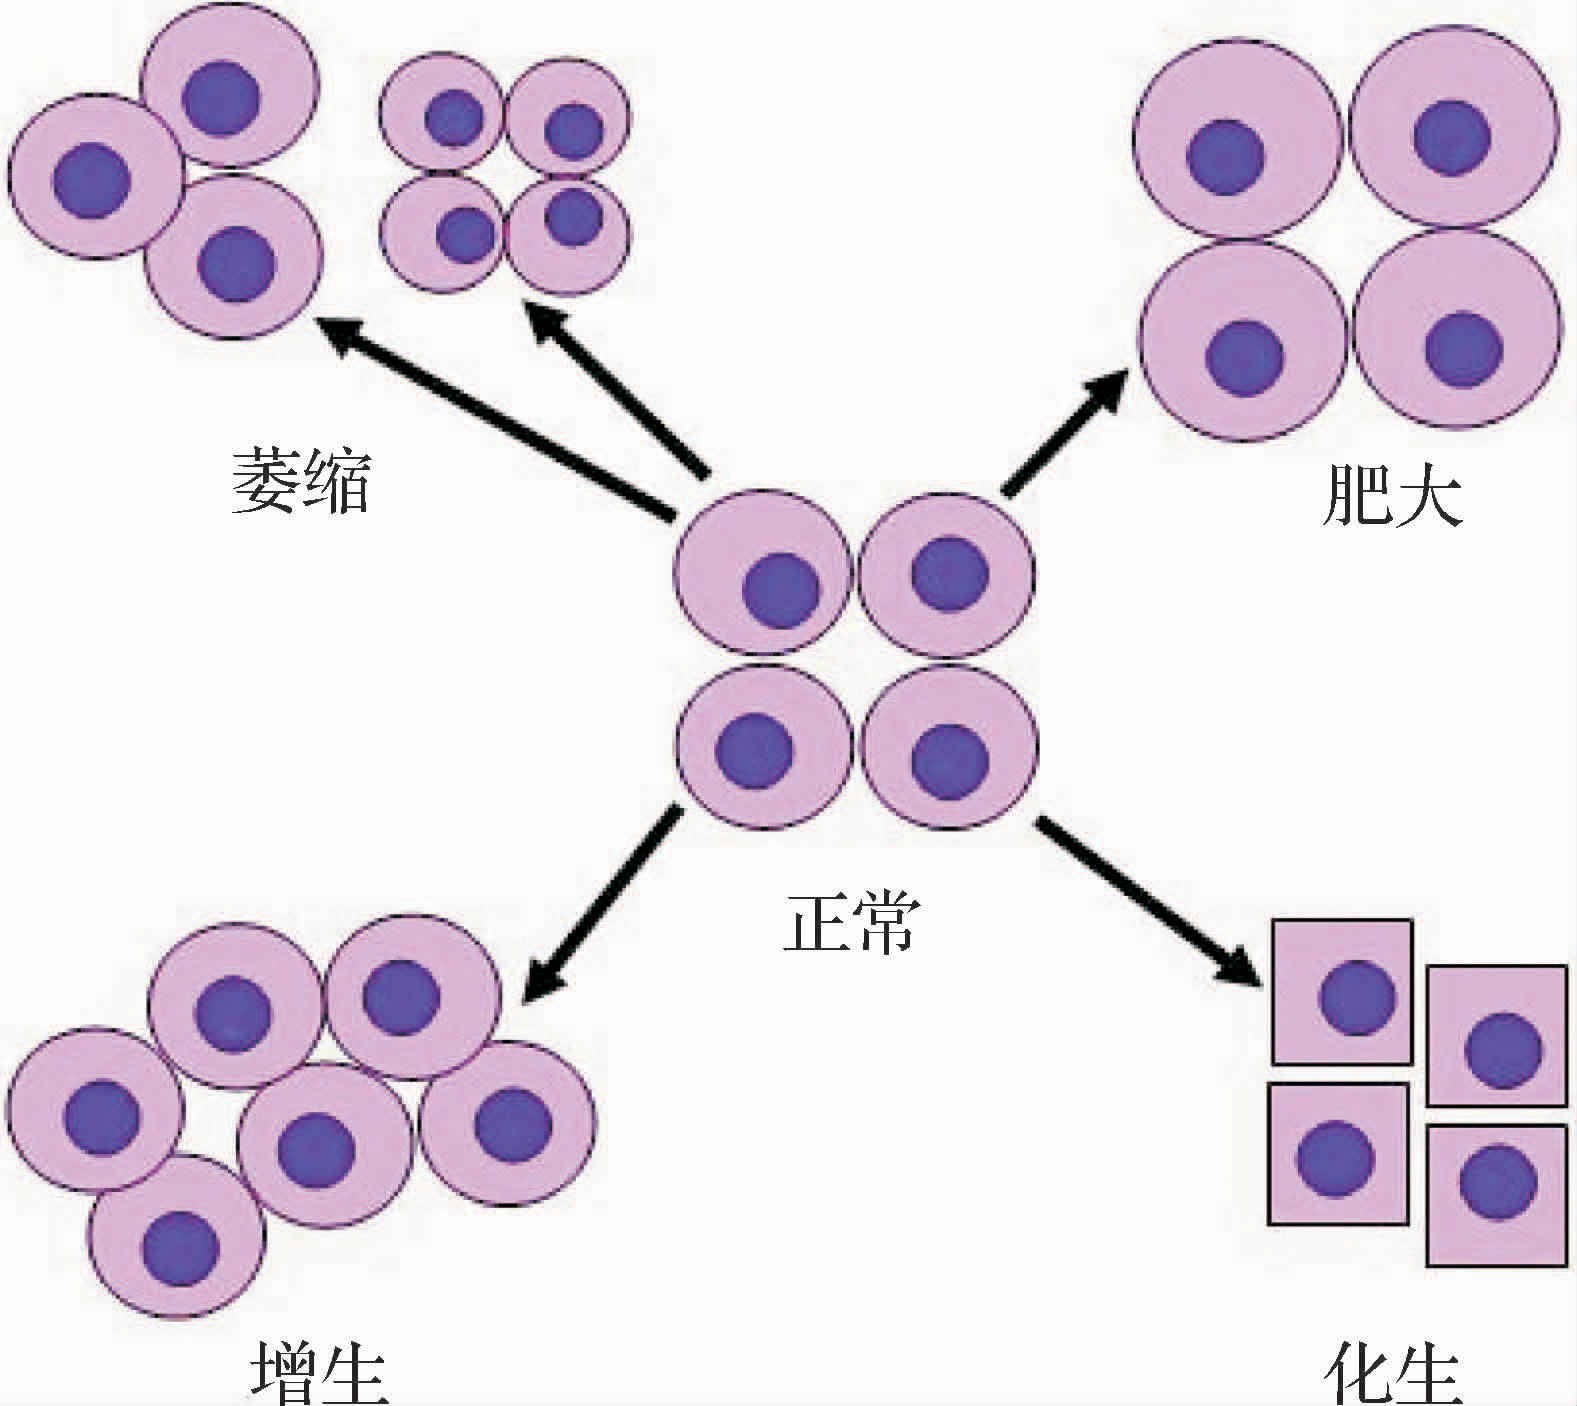
\includegraphics{./images/Image00005.jpg}
\end{table}

{2.预后营养指数(PNI)}
 PNI是由Mullen等对4种营养状态评价参数与外科手术病人预后的相关性进行了分析统计之后提出来的一种综合性营养评价方法。

PNI(%)=158-16.6(ALB)-0.78(TSF)-0.20(TFN)-5.80(DHST)

式中ALB为血清白蛋白(单位:g%);TSF为三头肌皮褶厚度(单位:mm);TFN为血清转铁蛋白(单位:mg%);DHST为迟发性超敏皮肤反应试验(硬结直径>5mm者,DHST=2;硬结直径<5mm者,DHST=1;无硬结反应者,DHST=0)。

评定标准:若PNI<30%,表示发生术后并发症及死亡的可能性均很小;若30%≤PNI<40%,表示存在轻度手术危险性;若40%≤PNI<50%,表示存在中度手术危险性;若PNI≥50%,表示发生术后并发症及死亡的可能性均较大。

Mullen等对161例非急诊手术病人的PNI测定调查显示,手术危险增加与术后并发症发生率及死亡率升高相关,其灵敏度为86%,特异性为69%。

{3.微型营养评定(MNA)}
 是一种简单、快速,适用于评价病人(特别是老年人)营养状况的方法,由Guigoz、Vallas和Garry于1994年提出。MNA评价内容包括: ①人体测量;②整体评定;③膳食问卷;④主观评定等。各项评分相加即得MNA总分。具体评价问卷内容如下所列(见[附])。

\begin{center}\rule{0.5\linewidth}{\linethickness}\end{center}

[附]

营养评价问卷

(一)姓名 性别 出生 年 月 日

(二)家庭住址

(三)原有疾病

(四)体重(kg) 身高(m) 血压(mm Hg)

1.筛选(按不同程度给予量化评分)

(1)既往3个月内是否有食欲下降、消化问题、咀嚼或吞咽困难而摄食减少?

0=食欲完全丧失□ 1=食欲中等度下降□ 2=食欲正常□

(2)既往3个月内体重下降

0=>3kg□ 1=不知道□ 2=1~3kg□ 3=无体重下降□

(3)活动能力

0=需卧床或长期坐着□ 1=能不依赖床或椅子,但不能外出□ 2=能独立外出□

(4)既往3个月内有无重大心理变化或急性疾病?

0=有□ 1=无□

(5)神经心理问题

0=严重智力减退或抑郁□ 1=轻度智力减退□ 2=无问题□

(6)BMI(kg/m\textsubscript{2} )

0=<19□ 1=19~<21□ 2=21~<23□ 3=≥23□

筛选总分(14):≥12正常,无需以下评价;≤11可能营养不良,继续以下评价

2.评价

(1)独立生活(无护理或不住院)?

0=否□ 1=是□

(2)每天应用处方药3种?

0=是□ 1=否□

(3)压疮(褥疮)或皮肤溃疡?

0=是□ 1=否□

(4)每天几次吃完全部饭菜?

0=1餐□ 1=2餐□ 2=3餐□

(5)蛋白质摄入情况:

*每天至少一份奶制品? A是□ B否□

*每周2份以上菜果或蛋? A是□ B否□

*每天肉、鱼或家禽? A是□ B否□

0.0=0或1个“是”□

0.5=2个“是”□

1.0=3个“是”□

(6)每天2份以上水果或蔬菜?

0=否□ 1=是□

(7)每天饮水量(水、果汁、咖啡、茶、奶等):

0.0=<3杯□ 0.5=3~5杯□ 1.0=>5杯□

(8)喂养方式:

0=无法独立进食□ 1=独立进食稍有困难□ 2=完全独立进食□

(9)自我评定营养状况:

0=营养不良□ 1=不能确定□ 2=营养良好□

(10)与同龄人相比,你如何评价自己的健康状况?

0.0=不太好□ 0.5=不知道□ 1.0=好□ 2.0=很好□

(11)中臂肌围(cm):

0.0=<21□ 0.5=21~22□ 1.0=≥22□

(12)腓肠肌围(cm):

0=<31□ 1=≥31□

评价总分(16):

筛选总分:

总分(30):

MNA分级标准:上述各项评分相加,若MNA≥24,表示营养状况良好;若17≤MNA≤23.5,表示存在发生营养不良的危险;若MNA<17,表示有确定的营养不良。

\begin{center}\rule{0.5\linewidth}{\linethickness}\end{center}

{4.住院病人预后指数(HPI)}

HPI=0.92(ALB)-1.00(DH)-1.44(SEP)+0.98(DX)-1.09

式中:ALB为血清白蛋白(单位:g/L);DH为延迟超敏皮肤试验(有1种或多种阳性反应,DH=1;所有均呈阳性,DH=2);SEP:败血症(有败血症,SEP=1;无败血症,SEP=2);DX表示诊断患有癌症(有癌,DX=1;无癌,DX=2)。

评价标准:若HPI为+1,表示有75%的生存概率;若HPI为0,表示有50%的生存概率;若HPI为-2,表示仅有10%的生存概率。

{5.营养风险指数(NRI)}
 美国退伍军人协会肠外营养协作研究组(VATPNCSG)于1991年在《新英格兰医学杂志》上首先提出NRI评价方法。NRI=10.7(ALB)+0.0039(TLC)+0.11(Zn)-0.044(Age)。

式中:ALB为血清白蛋白;TLC为淋巴细胞计数;Zn为血清锌水平;Age为年龄。

评定标准:若NRI>60,表示危险性低;若NRI≤55,表示存在高危险性。

Clugston等于2006年对梗阻性黄疸病人的研究表明,NRI风险升高与住院时间延长和死亡率增加相关。

完整的营养评价包括:疾病及饮食史、体格测量、生化指标、机体组成、营养平衡研究等。在营养评价过程中,体格测量与生化指标是营养评价的最常用方法,具有简单、方便、重复性好、能提供定量资料、不需要特殊仪器等特点。很多测量值与机体组成营养状况分析在统计学上具有显著相关性。然而,简单的体格测量和实验室检查常不能体现营养状况的急性改变,不能反映轻度和中度营养不良,也就不足以作为营养评价的唯一方法。同时,由于置信限较宽,敏感性和特异性差,更适用于流行病学人群调查,评价特定人群的营养状态。近年来,为了提高营养评价方法的敏感性和特异性,人们结合预后和大量的营养学指标,通过多因素回归分析,选择其中有意义的参数,组成最佳的预测模式,建立了多种营养评价方法,为营养状况评价提供了定性、定量的可信指标。

{参考文献}

[1]陶晔璇,徐远飞,汤庆娅,等.儿科病人入院时营养状况评价.中国临床营养杂志,2007,15(4):214~217

[2]蔡威.临床营养基础.第3版.上海:复旦大学出版社,2004,61~18

[3]Tienboon P. Nutrition problems of hospitalised children in a
developing country: Thailand. Asia Pacific J Clin Nutr, 2002, 11 (4):
258~262

[4]Renaudin P. Evaluation of the nutritional status of children less
than 5 years of age in Moundou, Chad: correlations with morbidity and
hospital mortality. Article in French. Med Trop(Mars), 1997, 57 (1):
49~54

[5]Hendricks KM, Duggan C, Gallagher L, et al. Malnutrition in
hospitalized pediatric patients. current prevalence. Arch Pediatr
Adolesc Med, 1995, 149: 1118~1122

[6]Ogden CL, Flegal KM, Carroll MD, et al. Prevalence and trends in
overweight among US children and adolescents, 1999~2000. JAMA, 2002,
288 (14): 1728~1732

[7]Ah SM, Selwyn BJ, Luby S, et al. Prevalence and correlates of
stunting among children in rural Pakistan. Pediatr Int, 2003, 45 (1):
49~53

[8]Jacobs DO, Wong M. Metabolic assessment. World J Surg, 2000, 24
(12): 1460~1467

[9]Phillips SM, Bandini LG, Compton DV, et al. A longitudinal
comparison of body composition by total body water and bioelectrical
impedance in adolescent girls. J Nutr, 2003, 133 (5): 1419~1425

[10]Kuczmarski RJ, Ogden CL, Guo SS, et al. 2000 CDC growth charts for
the United States: methods and development. Vital Health Stat 11, 2002,
(246): 1~190

[11]Ronald E. Pediatric nutrition handbook. 6th ed. American: American
Academy of Pediatrics, 2009, 559~576

\protect\hypertarget{text00003.html}{}{}


\chapter{颅脑}

\section{检查方法}

\subsection{常规检查}

横断面(或轴位)扫描:病人仰卧,有3个主要扫描平面。其扫描基线为:①听眦线(orbitomeatal
line,OML):亦称为眶耳线,简称OM线,即外眦至外耳孔中点的连线。②听眉线(superior
orbitomeatal
line,SML):亦称为上眶耳线,简称SM线,即眉毛上缘中点与外耳孔中点的连线。③瑞氏基底线(reid's
base
line,RBL):亦称人类学基线,简称RB线,即眶下缘与外耳孔中点的连线。检查幕上病变常用OM线;幕下病变常用SM线;眶内病变常用RB线。

冠状面扫描:病人仰卧或俯卧位,头部过伸,使冠状面与OM线垂直扫描。

\subsection{增强扫描}

一般认为,对急性颅脑外伤、急性卒中可只做平扫;对于脑瘤术后复查或只有增强检查才能显示病变的复查病例可只行造影增强;对于脑肿瘤、脑血管疾病、感染性疾病均需做增强扫描,外伤患者平扫正常时亦可行增强扫描。一般造影剂用量为60~100ml或儿童以2ml/kg用量,团注或快速滴注。

其显影机制分为两类:①血管内显影:如动脉瘤、动静脉畸形,其显影时间短,应注药后扫描或边注边扫。②血管外显影:强化机制在于血脑屏障的破坏(如胶质瘤)或血供丰富(如脑膜瘤、听神经瘤、脓肿壁)。由于垂体血供丰富,垂体增强扫描有利于缺乏血供的垂体瘤尤其微腺瘤的检出。

\subsection{脑池造影CT扫描}

造影剂可应用阳性非离子型水溶性碘造影剂(伊索显和欧乃派克等)和阴性造影剂(空气),后者主要用于小听神经瘤的诊断。一般阳性造影剂的用量为8~10ml,空气3~5ml,经腰穿注入。水溶性造影剂取头低脚高位或病变侧在低下部位,气体反之。一般注入造影剂15分钟后扫描,观察脑室多于6小时后扫描,延时的目的在于降低碘液浓度。如欲观察脑脊液的动力变化,则于注入造影剂2小时、6小时、12小时和24小时后进行扫描,必要时可于48小时或72小时后扫描。

\subsection{脑CT血管成像}

脑部CT血管成像或称为脑部CT血管造影(CT
angiography,CTA),是指经静脉注入造影剂后利用CT对包括靶血管在内的受检层面进行连续的薄层立体容积扫描,然后进行图像后处理,最终使靶血管立体显示的血管成像技术。

扫描从后床突下30mm开始,向上达后床突上50~60mm。其常用扫描参数如下:螺距1~2,层厚1~2mm,重建间隔1mm,造影剂用量(300mg/ml)80~120ml,注射流率2.5~3.5ml/s,延迟时间15~25秒。双层或多层螺旋CT可增加螺距、减小层厚,以取得更优质的图像。图像后处理可采用MIP、SSD和VR,以MIP最常用。

脑CT静脉成像(CT venography,CTV)扫描方法同上,只是扫描延迟时间为40秒。

CTA(包括CTV)可用于显示脑底动脉环(willis环)和大脑前、中、后动脉主干及其2~3
级分支血管;CTV
可显示大脑内静脉、大脑大静脉、皮质静脉、上矢状窦、直窦、横窦和乙状窦等。CTA(包括CTV)可用于动脉瘤、血管畸形(主要是AVM)、肿瘤血管、静脉病变及头皮血管瘤等的诊断。

\subsection{脑CT灌注成像}

CT灌注成像在中枢神经系统的应用包括:①作为颅外颈动脉或椎动脉闭塞性疾病的功能性检查方法,研究颅内血流量和侧支循环情况。②早期发现梗死或缺血,并显示其范围。③血管炎或继发性蛛网膜下腔出血时估计血管痉挛情况。④AVM估计分流情况。⑤研究肿瘤的血液灌注情况。

\subsubsection{检查技术}

CT灌注成像的质量受造影剂注射的总量、速度、患者的心功能状态以及CT扫描伪迹、部分容积效应等多种因素的影响。扫描时经肘静脉注射加热至37℃的造影剂40~50ml(儿童约为1ml/kg体重)。开始注射造影剂的同时启动快速动态扫描程序,以1层/秒的速度连续扫30~40秒以上,重建30~40幅灌注图像。注射流率多为8~9ml/s,最快达20ml/s,国内有学者采用2.5ml/s也获得较满意的CT灌注图像。通常包括最大强度投影(MIP)图、脑血流量(CBF)图、脑血容量(CBV)图、局部灌注达到峰值的时间(TTP)等图像。这些图像可通过数字化形式存储,均可彩色显示,以突出病变区域的对比度。

\subsubsection{灌注参数}

1.脑血容量(cerebral blood
volume,CBV):是指存在于一定量脑组织血管结构内的血容量,单位为ml/100g。根据时间-密度曲线下方封闭的面积计算得出。

2.脑血流量(cerebral blood
flow,CBF):CBF=CBV/MTT,指在单位时间内流经一定量脑组织血管结构的血流量,单位为ml/(100g·min)。它反映脑组织的血流量,CBF值越小意味着脑组织的血流量越低。正常值一般>50~60ml/(100g·min),<10~20ml/(100g·min)将导致膜泵衰竭和细胞死亡。

3.平均通过时间(mean transit
time,MTT):开始注射造影剂到时间-密度曲线下降至最高强化值一半的时间,主要反映的是造影剂通过毛细血管的时间,单位为秒(s)。

4.峰值时间(time to
peak,TTP):为开始注射造影剂至强化达到峰值的时间,由时间-密度曲线测得,单位为秒(s)。

此外,还有表面通透性(permeability of surface,PS)等参数。

\section{正常解剖和CT表现}

\subsection{颅盖软组织(头皮)}

颅盖软组织在额、顶、枕部分为皮肤、皮下组织、帽状腱膜、帽状腱膜下层和颅骨骨膜5层。前3层紧密连接,CT不能识别。帽状腱膜下层由疏松结缔组织构成,内含少量血管,CT呈低密度带,头皮裂伤出血亦在此层,如有化脓感染可蔓延到整个颅顶,并可经导静脉扩散到颅内。颅盖软组织在颞部则由皮肤、皮下组织、颞浅筋膜、颞深筋膜、颞肌和颅骨骨膜6层构成。

颅骨外膜CT不能识别,在颅缝处连接紧密并深入缝间成为缝间膜,故骨膜下血肿不超过此缝,并可据此与帽状腱膜下血肿相鉴别。

\subsection{脑颅骨和颅缝闭合的时间及顺序}

脑颅骨由枕骨、额骨、蝶骨、筛骨各一块及颞骨、顶骨各两块组成。颅骨分为3层,即外板、板障和内板。成人内外板CT表现为高密度,CT值>250Hu。新生儿板障为低密度,随年龄增长密度增加,50岁后板障层钙化与内外板融合为一层致密层。成人颅缝宽约0.5
mm。新生儿各骨之间为一片等密度的结缔组织膜相连,称为囟。

颅缝闭合约在30岁以后开始。一般矢状缝先闭合,继为冠状缝。而人字缝和枕骨乳突缝闭合最晚,且可终生不闭合。额缝在出生6个月后开始闭合,而在5~6岁时应完全闭合,此缝亦可终生存在。颅底缝多在出生时闭合,只有蝶枕缝到青春期闭合。

此外,应注意识别脑膜中动脉、板障静脉沟、静脉窦、导静脉、蛛网膜颗粒等常见的脉管压迹,以免误诊为骨折。

\subsection{颅底各颅窝的特点和孔道}

颅底骨内面由蝶骨嵴和颞骨岩部嵴分为前、中、后颅窝。

\subsubsection{各颅窝的结构特点}

1.前颅窝:筛骨板菲薄,外伤易造成骨折、损伤嗅神经及形成脑脊液漏。额骨眶板上面凹凸不平,脑外伤时底部的滑动易引起脑挫伤。

2.中颅窝:孔、洞较多,外伤骨折或肿瘤破坏通过这些结构引起相应的症状。如骨折累及蝶窦出现鼻出血、脑脊液鼻漏;岩锥骨折可损伤面神经和听神经;鼓室盖骨折引起脑脊液耳漏;脑膜中动脉损伤引起硬膜外血肿。

3.后颅窝:有大量肌肉覆盖,骨折较少见。但与颈段相连,可有畸形发生。

\subsubsection{。}

\begin{table}[htbp]
\centering
\caption{颅底主要孔道及内容物}
\label{tab2-1}
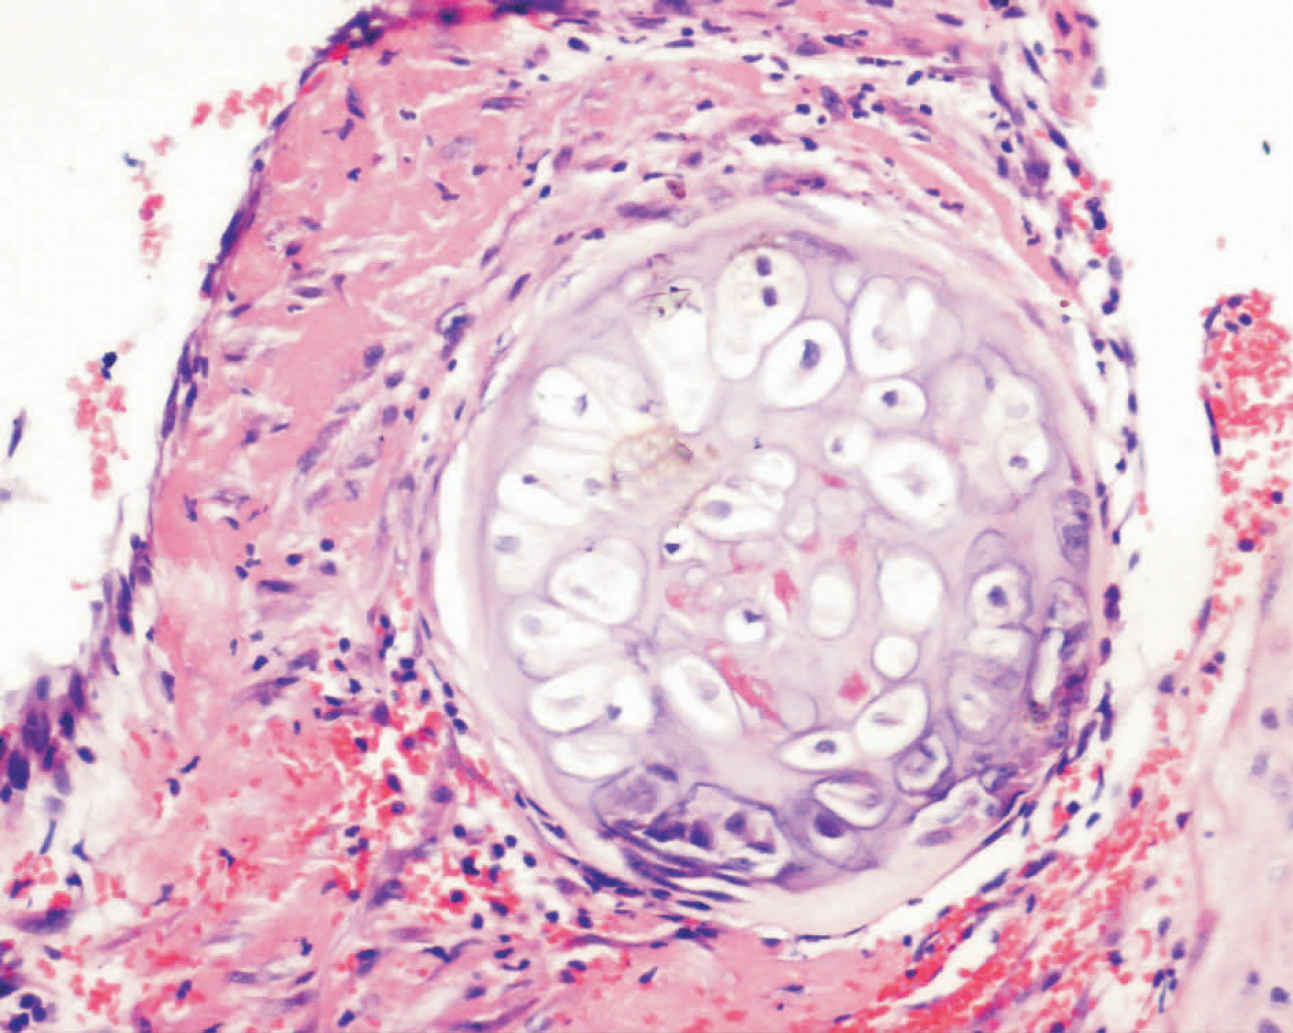
\includegraphics[width=\textwidth,height=\textheight,keepaspectratio]{./images/Image00004.jpg}
\end{table}

\subsection{脑膜}

脑的表面有3层被膜:①软脑膜:紧贴脑的表面,富血管、随脑回起伏。②蛛网膜:位于中层,由薄而透明、疏松成网的纤维构成,无血管结构(故增强扫描无强化),与硬脑膜走行一致。③硬脑膜:位于外层,由致密结缔组织构成,厚而坚韧,与颅骨内面的骨膜完全融合,故通常说硬脑膜为两层结构组成。正常CT不能直接显示3层结构。由于硬脑膜有丰富的血供且无血脑屏障,可以发生明显强化。

硬脑膜内层向颅腔内反折形成双层皱襞有支持、保护作用。主要形成物为:①大脑镰:前端附着于鸡冠,后缘呈水平形与小脑幕相续。大脑镰上、下缘两层分开分别形成上、下矢状窦。轴位像CT呈略高密度线状影,40岁后可钙化。②小脑幕:呈帐篷状分隔大脑枕叶和小脑。后方附着于枕骨横沟,两侧附着于岩椎,上缘正中与大脑镰相续,两侧前内缘形成小脑幕切迹,围绕中脑。轴位呈两侧对称的略高密度影,冠状位呈人字形线状略高密度影。③小脑镰:附着于枕内嵴上的一窄条状突起,分隔小脑半球。④其他:三叉神经半月节(Meckel腔)、海绵窦、直窦、横窦、乙状窦等。

\subsection{蛛网膜下腔和脑池}

脑蛛网膜在脑沟裂处不随之凹入,与软脑膜之间形成宽窄不一的蛛网膜下腔(或称蛛网膜下隙),内含脑脊液。某些局部宽大处称为脑池。主要的有:①大脑纵裂池;②胼胝体池;③小脑延髓池(又称枕大池
);④小脑溪(又称小脑谷);⑤延池;⑥桥池;⑦桥脑小脑角池;⑧脚间池;⑨视交叉池;⑩终板池;⑪外侧裂池;⑫环池;⑬四叠体池;⑭大脑大静脉池;⑮小脑上池(是四叠体池向后的延续);⑯帆间池(又称中间帆腔或第三脑室上池)。

鞍上池为CT和MR等轴位图像所特有。由于扫描体位的影响可呈:①六角星:前角为纵裂前部的后端(紧贴前角后端的横行部分主要是交叉池);两前外侧角为两外侧裂池;两后外侧角为围绕中脑的环池;后角为大脑脚间的脚间池(图\ref{fig2-1})。②五角星:与六角星不同的是,两后外侧角为围绕桥脑上部的桥小脑角池,后角不显示。鞍上池前方是额叶底部直回,两侧壁是颞叶海马钩回,后方为大脑脚或桥脑上部。

\begin{figure}[!htbp]
 \centering
 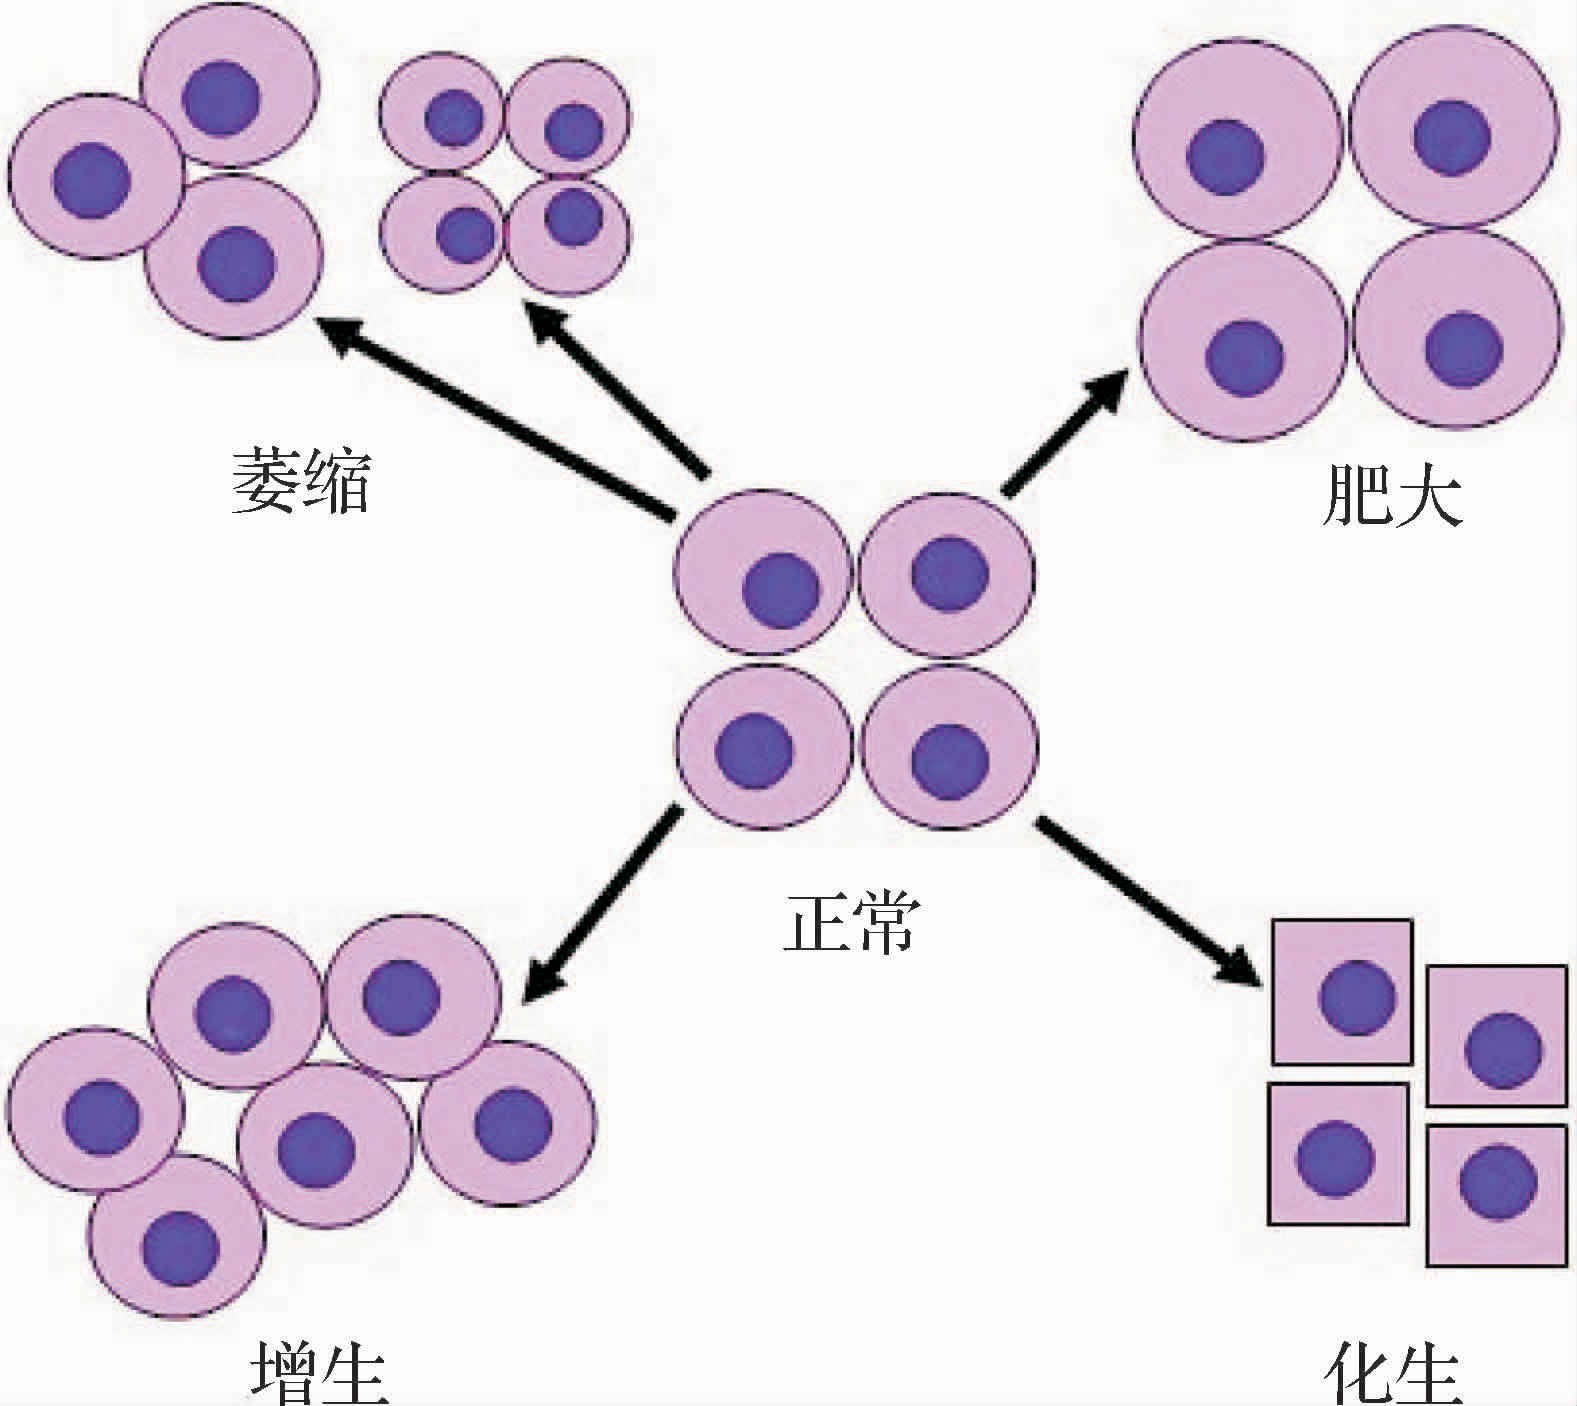
\includegraphics[width=.7\textwidth,height=\textheight,keepaspectratio]{./images/Image00005.jpg}
 \captionsetup{justification=centering}
 \caption{鞍上池 \\{\small 呈六角形水样密度区}}
 \label{fig2-1}
  \end{figure} 



鞍上池内前部可见两条视束,横径约12mm,前后径约8mm,外侧可见两条颈内动脉,中央可见垂体柄,正常垂体柄粗<4mm。

帆间池与第三脑室顶部的区别:帆间池位于第三脑室顶的上方、穹隆体和穹隆连合的下方,呈尖向前的三角区,两前外侧界为穹隆的内侧缘,后界为胼胝体压部。与第三脑室的区别为:①帆间池的层面较第三脑室顶高;②帆间池后界为胼胝体压部,而第三脑室顶部的后界为松果体;③帆间池前部的尖不与侧脑室相连,而第三脑室前端可达侧脑室前角。

此外,枕大池可发育巨大(但一般不产生临床症状)呈对称性和非对称性。结合其有无张力、颅骨有无压迹等可与蛛网膜囊肿相鉴别(图\ref{fig2-2}),有文献将其列入发育异常。因终板较薄不显影,常看到终板池与第三脑室下部相通的假象。小脑溪位于两侧小脑扁桃体之间,呈一细长的间隙,后通小脑延髓池,前通第四脑室。

\begin{figure}[!htbp]
 \centering
 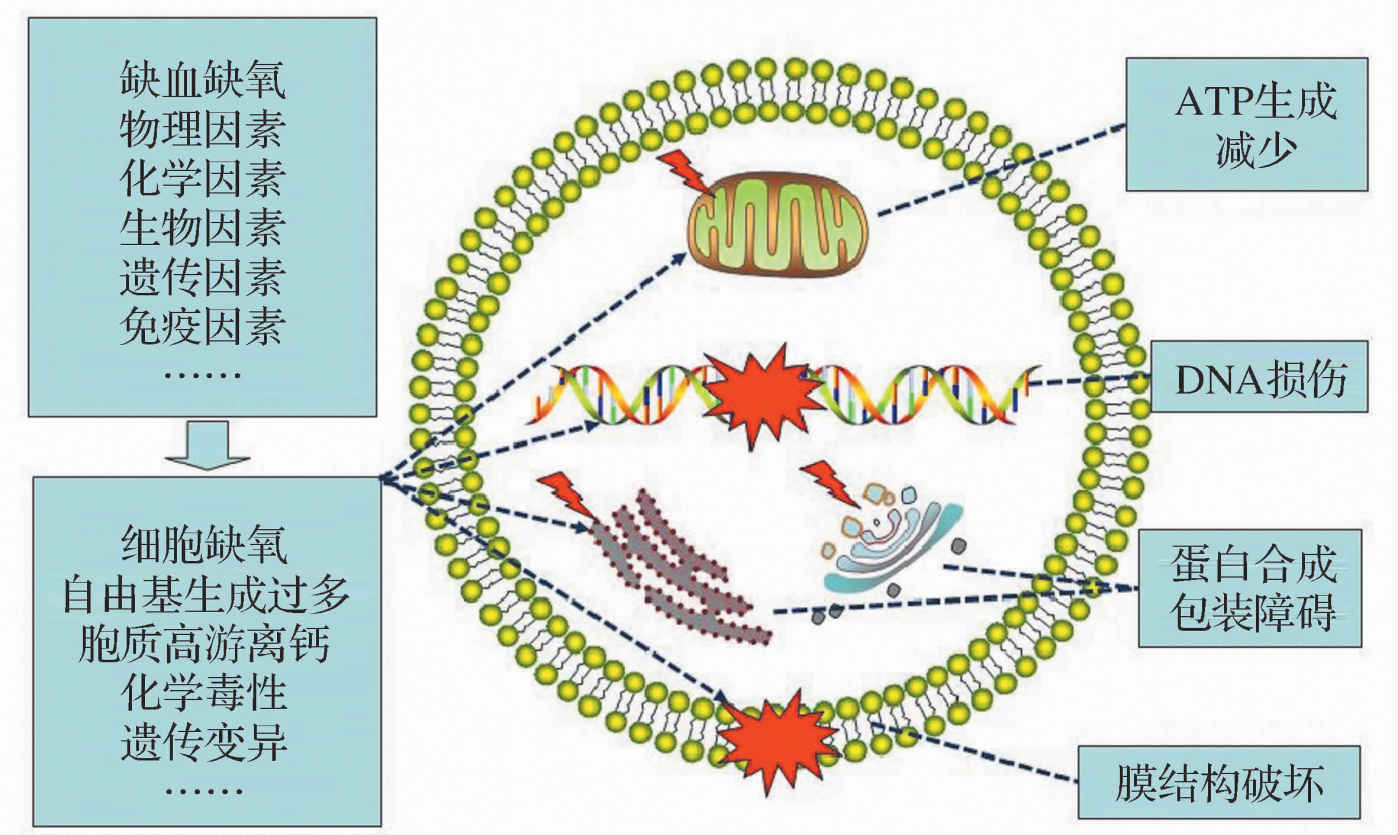
\includegraphics[width=.7\textwidth,height=\textheight,keepaspectratio]{./images/Image00006.jpg}
 \captionsetup{justification=centering}
 \caption{巨大枕大池 \\{\small 显示枕骨内板下至岩锥后缘有新月形水样密度区}}
 \label{fig2-2}
  \end{figure} 


\subsection{大脑半球的分叶及边缘系统}

分叶:大脑由中线的半球间裂分为左右两半,中间由胼胝体相连。大脑半球由脑沟裂分为下列5叶。①额叶:位于前上部。内侧以纵裂和大脑镰与对侧分开,后方由中央沟与顶叶分开,外下方经外侧裂与颞叶分开,前下方为额骨和眶顶。②颞叶:经外侧裂垂直部和水平部与额叶分开。顶枕裂(沟)与枕前切迹(枕极前4~5mm)的连线为颞、枕叶的分界。③顶叶:经中央沟与前方的额叶分开,下方以外侧裂与颞叶分开,后方以顶枕沟与枕叶分开。④枕叶:经顶枕沟与顶叶分开,与颞叶的分界线为顶枕沟与枕前切迹的连线。⑤岛叶:隐藏于外侧裂深部的近三角形的独立区域,四周有环形沟,由额、顶、颞叶皮质沿外侧裂深部凹入形成岛盖。

边缘系统:大脑半球内侧面的扣带回、海马回、钩回、海马、杏仁核等相连构成一个弯弓形脑回,因位置在大脑和间脑交界处的边缘,所以称为边缘系统或边缘叶。通过控制下丘脑来调节内脏及情绪活动。

此外,颞、顶、枕叶的分界线是假设的,因此很不清楚,这一区域也称为颞顶枕交界区。

\subsection{大脑半球的白质}

\subsubsection{半卵圆中心}

髓质占大脑半球的大部分,较厚的皮质下纤维在横断面图像、侧脑室上层面呈半卵圆形,故称为半卵圆中心,是影像学的一个概念。

\subsubsection{大脑白质纤维分类}

大脑白质的纤维结构复杂,大体分为以下3种:

1.联络纤维:在一侧半球内部各回、各叶间的往返纤维称为联络纤维。短的是联系在相邻脑回之间的弓状纤维;长的是联系在各叶皮质间的纤维,如钩束、扣带束、上纵束、下纵束及枕额上、下束等。

2.连合纤维:指联系左右半球的纤维,主要有胼胝体、前联合和海马联合等。①胼胝体:位于大脑纵裂底部,呈拱桥状。前端弯向腹后方称嘴,由嘴向前上方弯曲部称为膝,由膝向后延伸为体部(构成侧脑室壁的大部分),后端较厚称为压部。②前联合:位于胼胝体嘴的后下方,呈卵圆形,是两半球的嗅球和海马旁回的联合。

3.投射纤维:大脑皮层与其下部的间脑、基底节、脑干和脊髓的连接纤维称为投射纤维。包括内囊、穹隆、外囊和最外囊。①内囊:两侧内囊横断面呈“><”型,中央顶点为膝,前后分别为前肢和后肢。内囊位于丘脑、尾状核和豆状核之间。内囊后肢边缘模糊的低密度区(约位于膝部到豆状核后缘距离的2/3~3/4处)为正常皮质脊髓束,勿误为缺血灶。②外囊:在豆状核外,居豆状核和屏状核之间,两侧在横断面呈“()”型。③最外囊:位屏状核外侧,岛叶内侧,CT难以显示。

\subsection{基底节}

基底节包括尾状核、豆状核、屏状核和杏仁核。其中豆状核有两个白质板将其分为3部分,外部最大称为壳,内侧两部分称为苍白球。但CT不能显示其白质板。尾状核和豆状核合称为纹状体,与维持肌张力及运动频率有关。杏仁核与情绪变化有关。

\subsection{间脑}

间脑(通常将端脑和间脑合称为大脑)连接大脑半球和中脑,包括以下4部分。

1.丘脑:为一大卵圆形核团。内侧构成侧脑室侧壁,借中间块使左右丘脑相连;其外侧为内囊后肢;其前端尖圆为丘脑结节;后端圆钝为丘脑枕;丘脑枕的外下部有两个隆起为内、外侧膝状体。丘脑是各种感觉体传向大脑皮层的中间站。

2.下丘脑:构成侧脑室底和侧壁的一部分,包括视交叉、漏斗、灰结节、乳头体和垂体神经部。它是皮质下植物神经中枢,并通过下丘脑---垂体柄和垂体门脉系统调节垂体功能。

3.底丘脑:为丘脑和中脑的移行区。接受来自苍白球和运动区的纤维,并发出纤维到达红核、黑质及中脑被盖,功能上与苍白球密切相关。

4.上丘脑:位于三脑室后部,包括丘脑髓纹、缰三角和松果体,参与嗅反射通路。松果体为一退化的内分泌结构,分泌抑制青春期激素。松果体呈锥形,长5~8mm,宽4mm,向左偏移1~2mm是正常现象,但向右偏移却有病理意义。CT扫描75%以上成人于三脑室后部可显示松果体与缰联合钙化。缰联合钙化居前,范围不超过1cm;松果体钙化居后,一般不超过5mm。

此外,有文献将内、外侧膝状体称为后丘脑。

\subsection{脑干}

脑干上接间脑,下续颈髓,与小脑之上、中、下脚相连,分为以下3部分。

1.中脑:在间脑和脑桥之间,从前向后为大脑脚、被盖和四叠体(顶盖)组成。大脑脚与被盖之间以黑质为界;被盖与四叠体之间以中脑导水管为界。腹侧两束粗大的纵行纤维为大脑脚,其间形成脚间窝,动眼神经从脚间窝出脑。中脑背部有上丘和下丘两对隆起总称为四叠体。上、下丘分别与外、内侧膝状体借上、下丘臂相连,分别是皮质下视觉和听觉反射中枢。下丘后方连接前髓帆,滑车神经自下丘下方发出。

2.桥脑:桥脑在中脑的下方,从前向后为基底部和被盖部。前面正中浅沟内可见基底动脉。横行基底部的纤维向两侧聚成脑桥臂,经小脑中脚进入小脑。基底部与桥臂之间有三叉神经发出。桥脑腹侧与延髓交界的沟内,由内向外有外展神经、面神经和前庭蜗神经发出。桥脑背面下半部即菱形窝的上半部为第四脑室底(CT轴位第四脑室前为桥脑)。

3.延髓:上接桥脑,下续颈髓。腹侧面中线(前正中裂)两旁有锥体(由皮质脊髓束和皮质脑干束组成)。在延髓的下方由纤维交叉形成锥体交叉。锥体外侧有椭圆形隆起称为橄榄。锥体和橄榄之间有舌下神经穿出。橄榄背侧自上而下依次有舌咽神经、迷走神经和副神经根发出。

\subsection{小脑和小脑核}

小脑位于桥脑和延髓的后方,中间相隔第四脑室。小脑正中的蚓部与两侧小脑半球间无明显分界。小脑半球下面近枕骨大孔部分突出称为小脑扁桃体。小脑前后均向内凹称为小脑前切迹和后切迹。小脑半球借上、中、下脚分别与中脑背侧、桥脑腹侧和延髓的背侧相连接,小脑表面为灰质,内部为白质。

小脑白质内有灰质团块,称为小脑中央核。共有4对,分别为齿状核、顶核、栓状核、球状核。其中齿状核最大,位于小脑半球的中心部,是小脑传出纤维的主要发起核。

\subsection{脑室系统}

1.侧脑室:左右各一,分为以下5部分:①前角:又称额角,位于额叶内,在室间孔以前。顶为胼胝体,内侧壁是透明隔,倾斜的底及外侧壁为尾状核头。②体部:位于顶叶内,由室间孔至三角部。顶为胼胝体体部;内侧壁是透明隔;底由外侧到内侧分别为尾状核体、丘脑背面终纹、丘脑上面的外侧部、脉络丛和穹隆外侧缘。③三角区:即体、后角、下角分界处,内容脉络球。CT上是区分颞、枕、顶叶的标志。④后角:又称枕角,位于枕叶内,形状变异很大,有时缺如。顶和外侧壁由胼胝体放散形成;内侧壁上有两个纵行膨大,上方的称后角球(由胼胝体大钳构成),下方的称禽距。⑤下角:在颞叶内,又称颞角。在丘脑后方弯向下,再向前进入颞叶。顶大部分由胼胝体构成,内侧小部分由尾状核尾和终纹构成,底由内至外为海马伞、海马和侧副隆起。

正常成人两侧前角之间的距离<45mm,前角间最大距离与头颅最大内径之比<35%,在2岁以下其比值应<29%,两侧尾状核内缘之间的距离<25mm,为15mm左右。

2.第三脑室:两侧间脑间的狭窄腔隙。成人男性宽为2.8~5.9mm,女性为2.5~5.3mm。经室间孔与左右侧脑室相通,后经中脑导水管与第四脑室相通。顶有第三脑室脉络丛;底为下丘脑;前壁为前联合和终板;后壁为缰联合、松果体和后联合。

3.第四脑室:腹侧为桥脑和延髓,背侧为小脑,上接中脑导水管,下续脊髓中央管。经侧孔与桥脑小脑角池相通;经下端正中孔与小脑延髓池相通。第四脑室底为菱形窝,顶为前髓帆和后髓帆,呈马蹄形,宽(前后径)约9mm。

4.中脑导水管:位于中脑背侧,是中脑被盖和四叠体的分界,长约7~18mm,直径约1~2mm。正常CT难以显示。

此外,第五、第六脑室即透明隔间腔和穹隆间腔属两种解剖变异。但第五脑室如积液过多,向外膨隆并影响室间孔的引流,可称为透明隔囊肿。

\subsection{静脉和静脉窦}

\subsubsection{脑动脉}

脑的血供来自颈内动脉和椎动脉,前者供应大脑半球的前2/3,后者供应脑干、小脑和大脑半球的后1/3。

1.大脑前动脉:供应额、顶叶近中线内侧面约1.5cm的范围,呈长条形。其水平段分出细小前穿质动脉供应尾状核头、壳核和内囊前部,另有部分供应下丘脑。

2.大脑中动脉:皮质支供应额、顶、颞叶的外表面大部分。中央支供应尾状核和壳核的一部分,以及苍白球、内囊前后肢,称为豆纹动脉。

3.大脑后动脉:供应枕叶和颞叶底面,中央支供应部分间脑。

4.椎基动脉:两侧椎动脉在延髓腹侧汇合为基底动脉。基底动脉走行于桥脑前面,到脚间池分为左右大脑后动脉。基底动脉分出成对的桥脑支、内听道支、小脑前支和小脑上支。小脑后支来自椎动脉。

颅底动脉环即Willis环,由前交通动脉、两侧大脑前动脉、两侧后交通动脉和大脑后动脉相互吻合构成的六角形动脉环,是沟通两侧颈内动脉和椎动脉的侧支循环通路。其变异较大,完整者仅占53.8%。

\subsubsection{脑静脉}

大脑半球静脉分为深、浅两组。①浅静脉:收集大脑皮质和白质浅层的静脉血,包括大脑上静脉、大脑中静脉和大脑下静脉分别汇入上矢状窦、海绵窦、横窦、岩上窦和岩下窦,其间有吻合静脉相沟通。②深静脉:主要收集脑深部的血液。透明隔静脉和纹丘静脉在室间孔后缘汇合成大脑内静脉,两侧的大脑内静脉以及基底静脉在松果体后方汇合成大脑大静脉。大脑大静脉与下矢状窦相连终于直窦。

\subsubsection{静脉窦}

在两层硬脑膜之间引流静脉血液入颈内静脉,包括上矢状窦、下矢状窦、直窦、横窦、海绵窦、岩上窦、岩下窦和乙状窦。其中海绵窦位于蝶鞍两侧高约5~8mm,横径5~7mm,前后径为10~15mm,增强后呈高密度,平扫不易显示。

\subsection{Brodmann功能定位区和大脑皮质的主要功能区}

正常脑皮质的密度高于髓质,易于分辨。脑皮质CT值为32~40Hu,脑髓质CT值为28~32Hu,两者平均相差(7.0±1.3)Hu。含脑脊液的间隙为水样密度,CT值为0~20Hu。

图\ref{fig2-3}A~I为正常颅脑CT轴位像,按Brodmann功能定位法共分47个区。如图\ref{fig2-3}A~I和图\ref{fig2-4}A、B、C、D所示,大脑皮质主要的功能区定位如下:

1.第Ⅰ躯体感觉区:位于中央后回和中央旁小叶的后半,主要是3、1、2区。

2.第Ⅰ躯体运动区:位于中央前回和中央旁小叶的前半,主要是4区。

3.视觉区:位于枕叶内侧面,距状裂(沟)两侧,包括舌回和楔叶的一部分,即17、18、19区。

4.听区:位于颞横回,主要是42区,接受听辐射的投射。其特点是一侧听区接受双侧的听觉冲动传入,但以对侧为主。故一侧听区损伤,可使双侧听力下降,但不会完全耳聋。

5.味觉区:在中央后回下端。

6.语言中枢:在左侧半球的皮质产生了4个分析区,总称为语言中枢。①说话中枢:在额下回后部,即44区。此区损伤产生失语症。②书写中枢:位于额中回后部。此区损伤产生失写症。③阅读中枢:位于顶下小叶的角回,即39区。此区损伤产生失读症。④听话中枢:在颞上回后部。功能是理解别人的语言和监听自己所说的话。此区损伤,对听到的语言不能理解,自己说话错误、混乱而不自知,称为感觉性失语症。

7.其他:5、7区为触摸识别物体的实体感觉皮质区,为顶上小叶。额上回从前向后为9、8、6区。8区和枕叶19区为皮质眼球运动区,受刺激时产生双眼向对侧同向偏盲。8和6区为锥体外系皮质区,与共济运动有关。9、10、11区为额叶联合区,与智力和精神活动密切相关。40区位于顶下小叶缘上回,优势半球为运用中枢,是人类后天经复杂的动作和劳动技能所建立的运动区。损伤后,手的运动功能正常,但不能完成过去掌握的复杂动作和操作技法。


\begin{figure}
  \centering
  \subfloat[经海绵窦层面]{
  \begin{minipage}[b]{0.7\textwidth}
    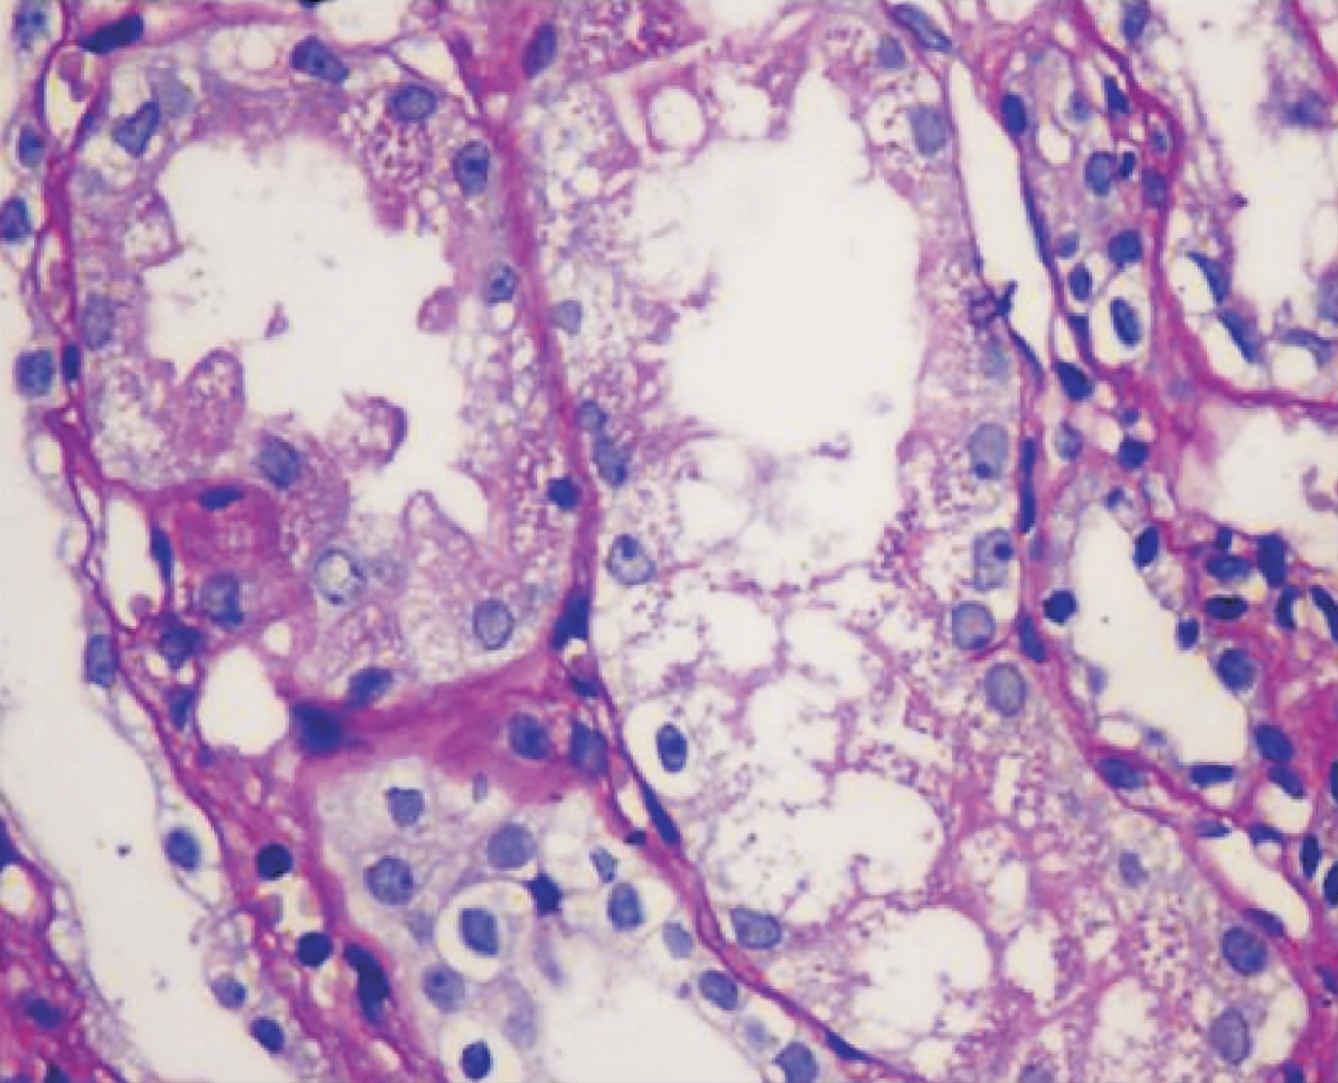
\includegraphics{./images/Image00007.jpg}
  \end{minipage}}\\
  \subfloat[经鞍上池层面]{
  \begin{minipage}[b]{0.7\textwidth}
    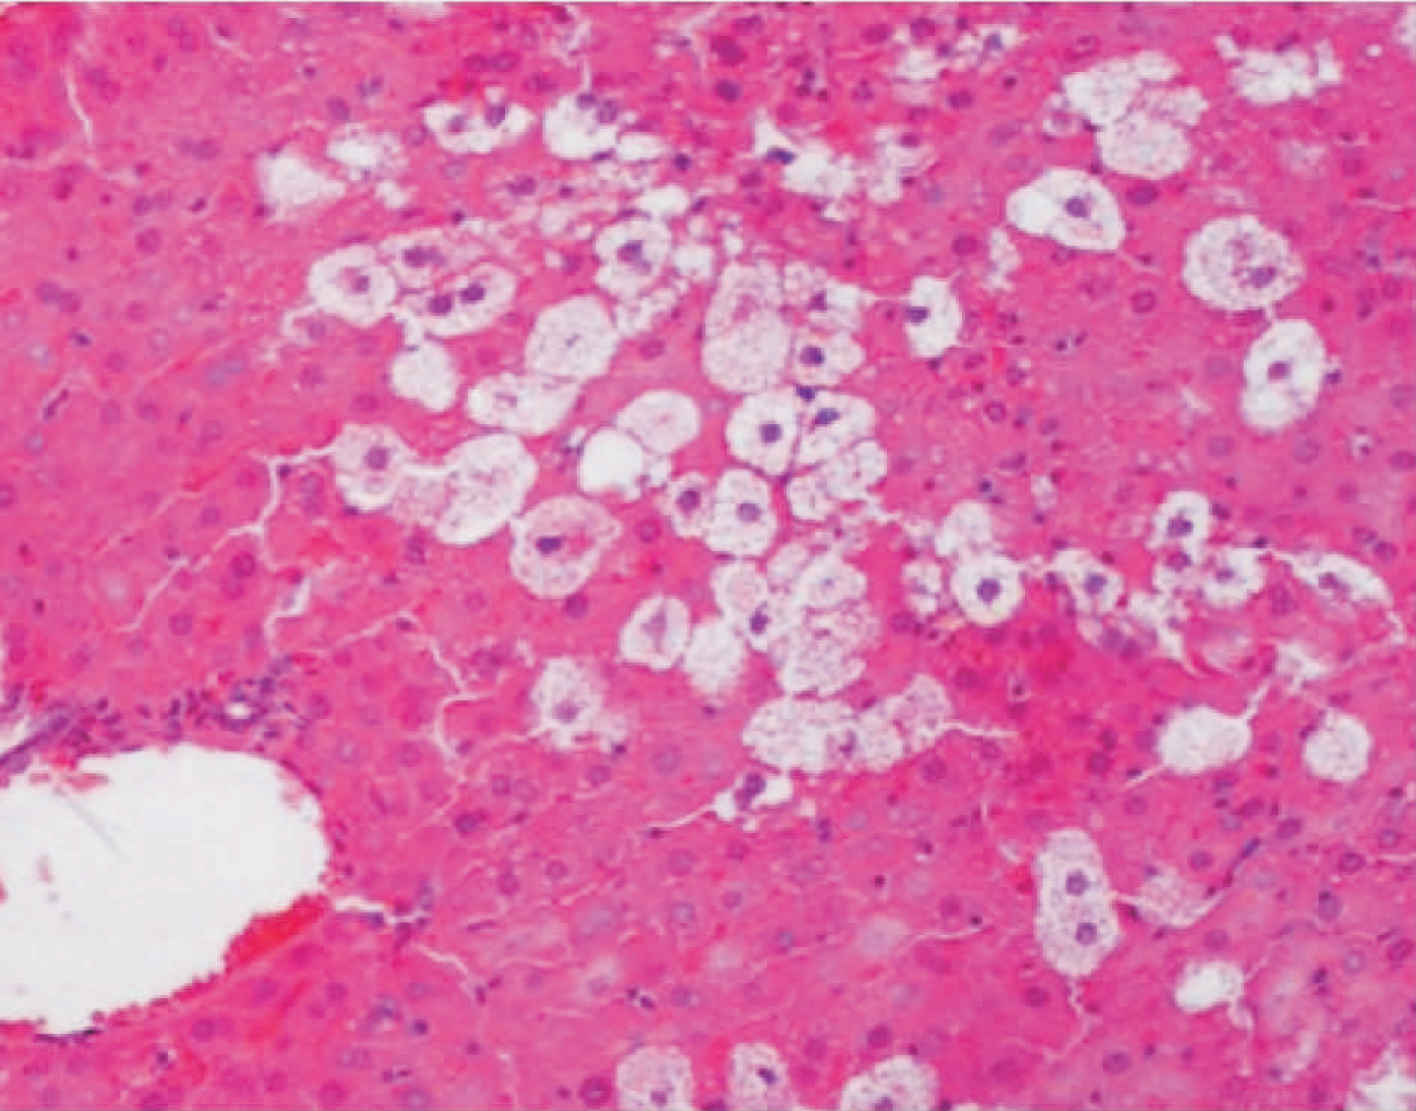
\includegraphics{./images/Image00008.jpg}
  \end{minipage}}\\
  \subfloat[经三脑室下部层面]{
  \begin{minipage}[b]{0.7\textwidth}
    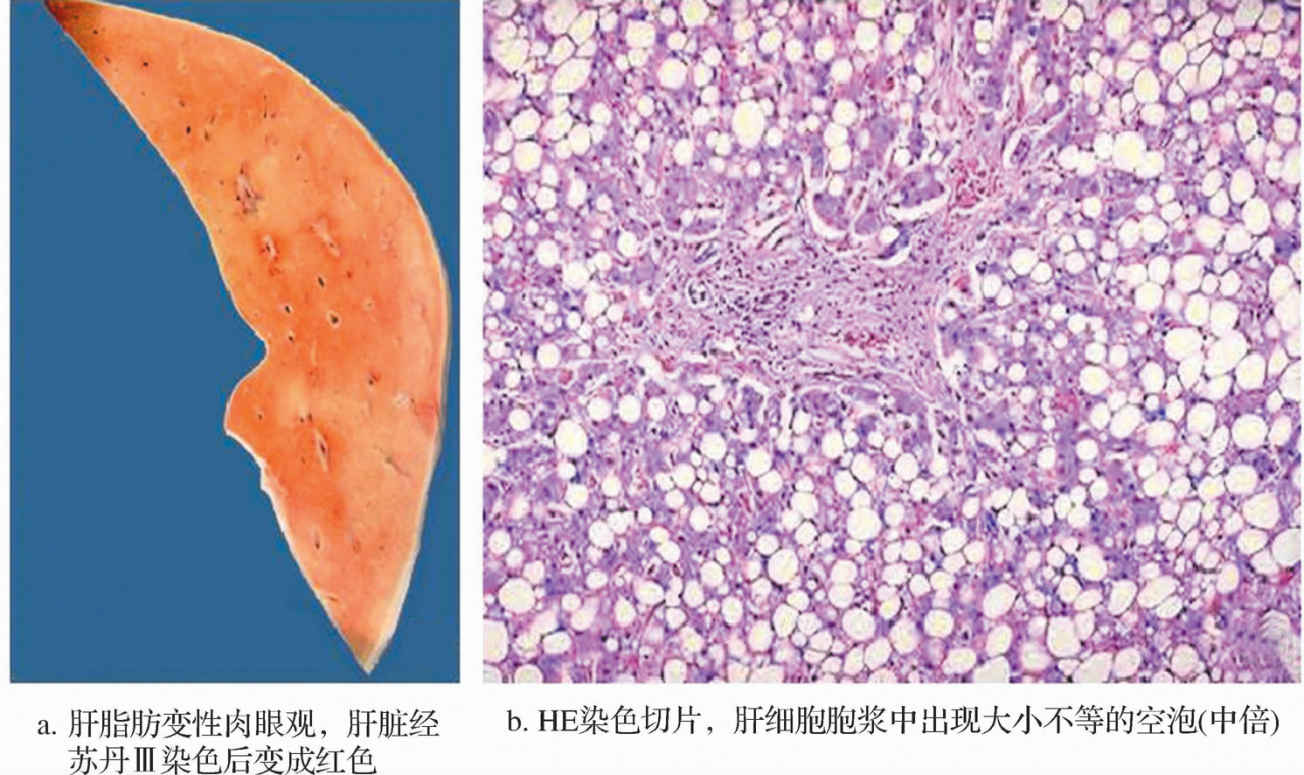
\includegraphics{./images/Image00009.jpg}
  \end{minipage}}
  \caption{}
  \label{fig2-3}
  \end{figure}

  \begin{figure}
    \ContinuedFloat             %%<-- put this in subsequest figures.
    \centering
    \subfloat[经松果体层面]{
      \begin{minipage}[b]{0.7\textwidth}
        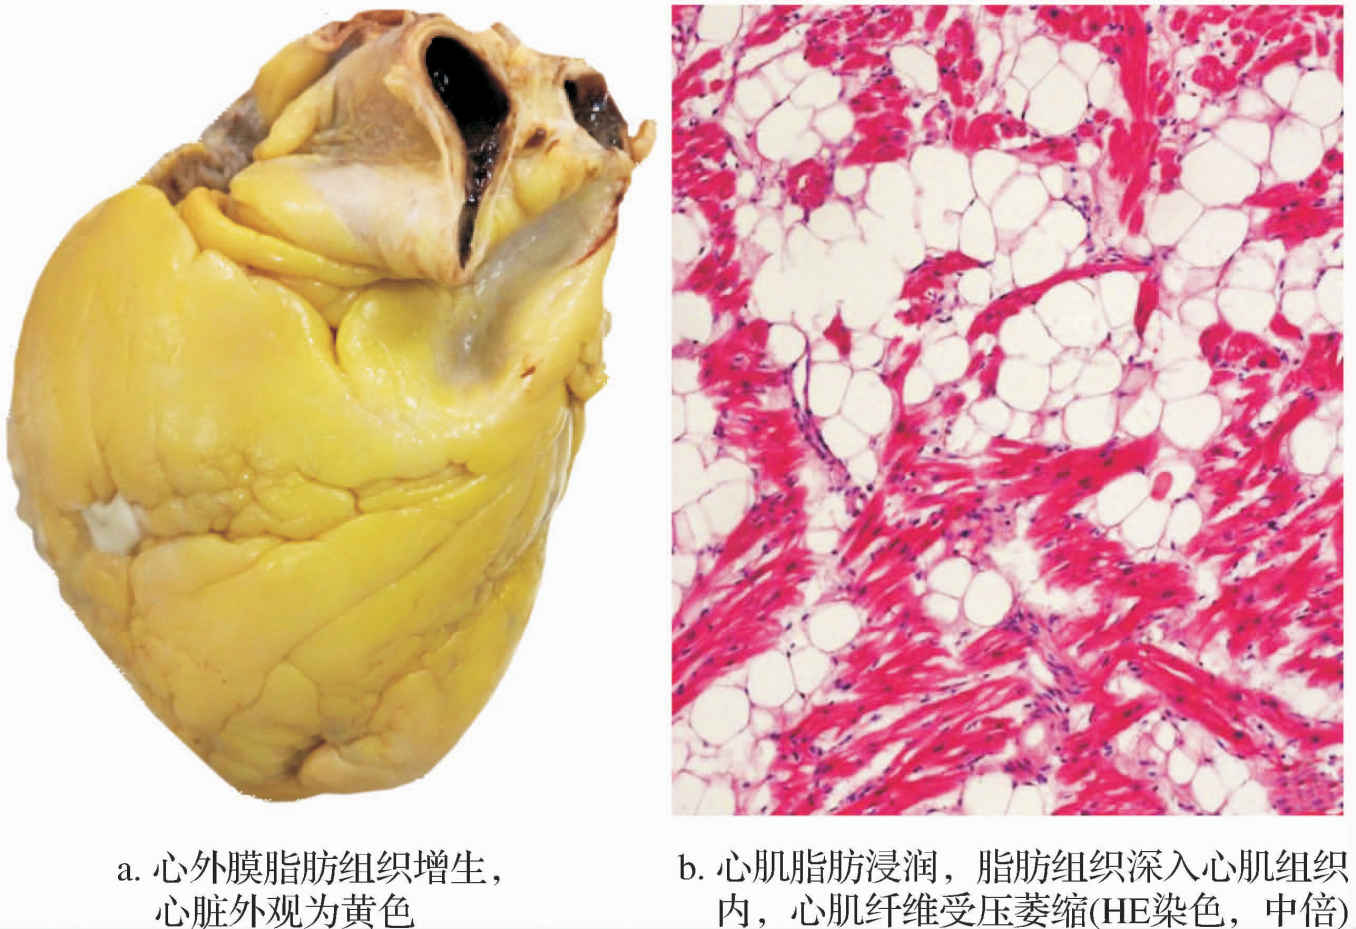
\includegraphics{./images/Image00010.jpg}
      \end{minipage}}\\
      \subfloat[经三脑室上部层面]{
      \begin{minipage}[b]{0.7\textwidth}
        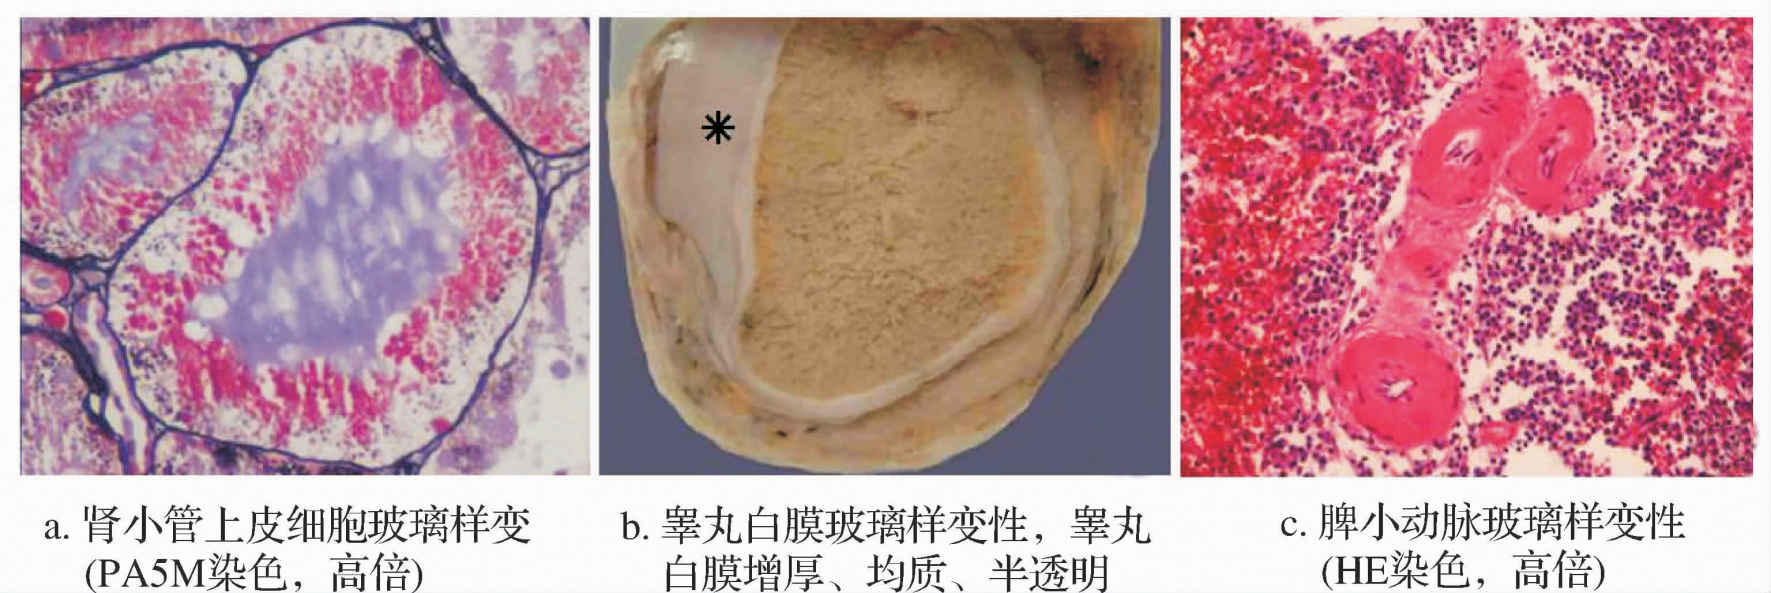
\includegraphics{./images/Image00011.jpg}
      \end{minipage}}\\
      \subfloat[经侧脑室体部层面]{
      \begin{minipage}[b]{0.7\textwidth}
        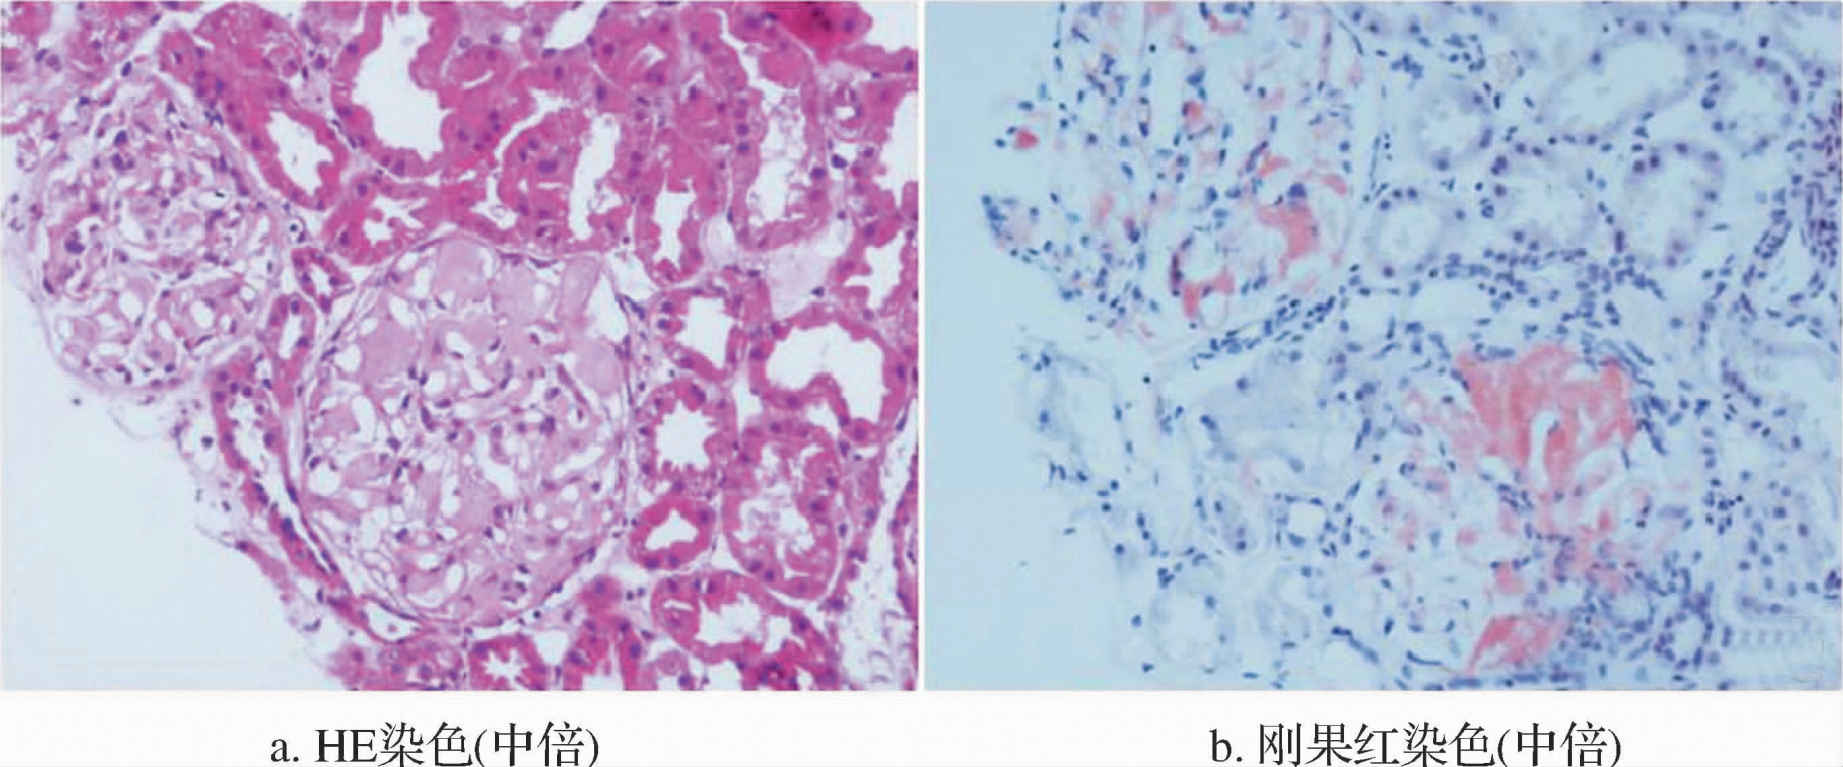
\includegraphics{./images/Image00012.jpg}
      \end{minipage}}
      \caption[]{}
  \end{figure}

  \begin{figure}
    \ContinuedFloat             %%<-- put this in subsequest figures.
    \centering
    \subfloat[经胼胝体体部层面]{
      \begin{minipage}[b]{0.7\textwidth}
        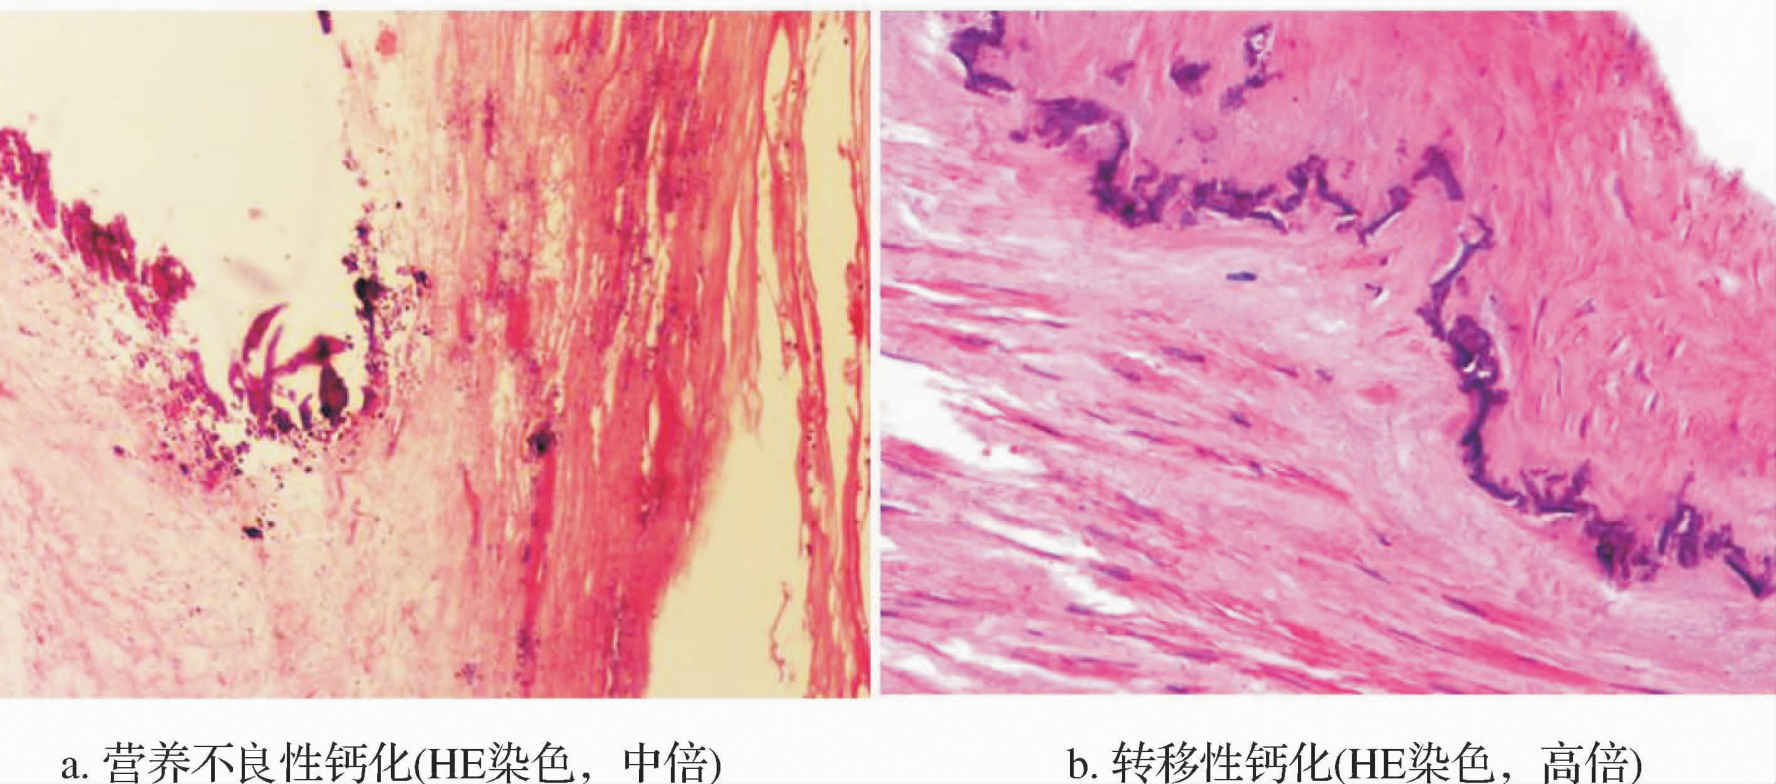
\includegraphics{./images/Image00013.jpg}
      \end{minipage}}\\
      \subfloat[半卵圆中心层面]{
      \begin{minipage}[b]{0.7\textwidth}
        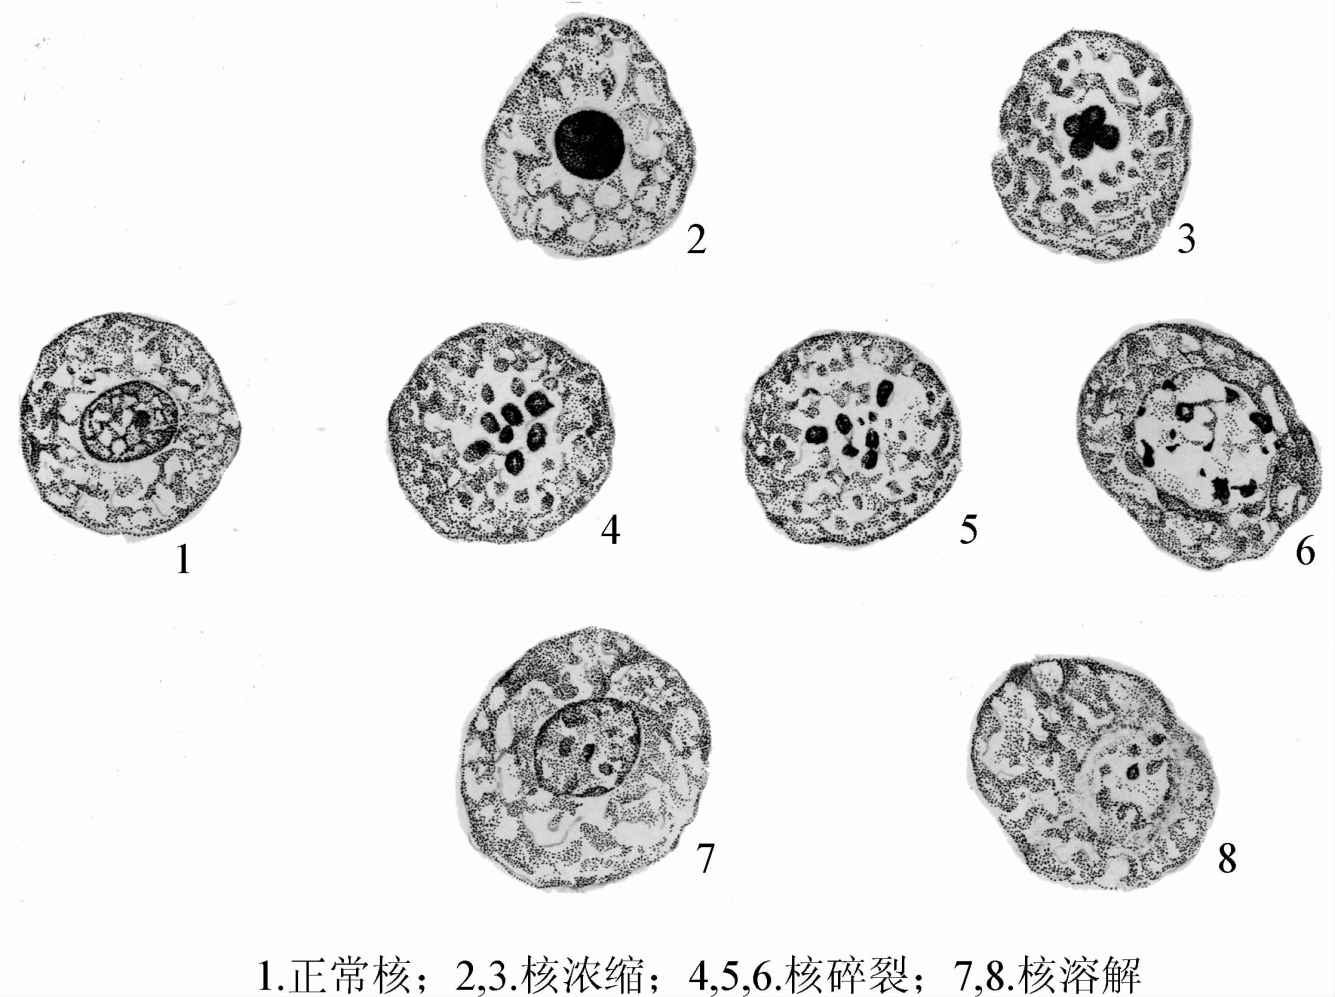
\includegraphics{./images/Image00014.jpg}
      \end{minipage}}\\
      \subfloat[半卵圆中心以上层面]{
      \begin{minipage}[b]{0.7\textwidth}
        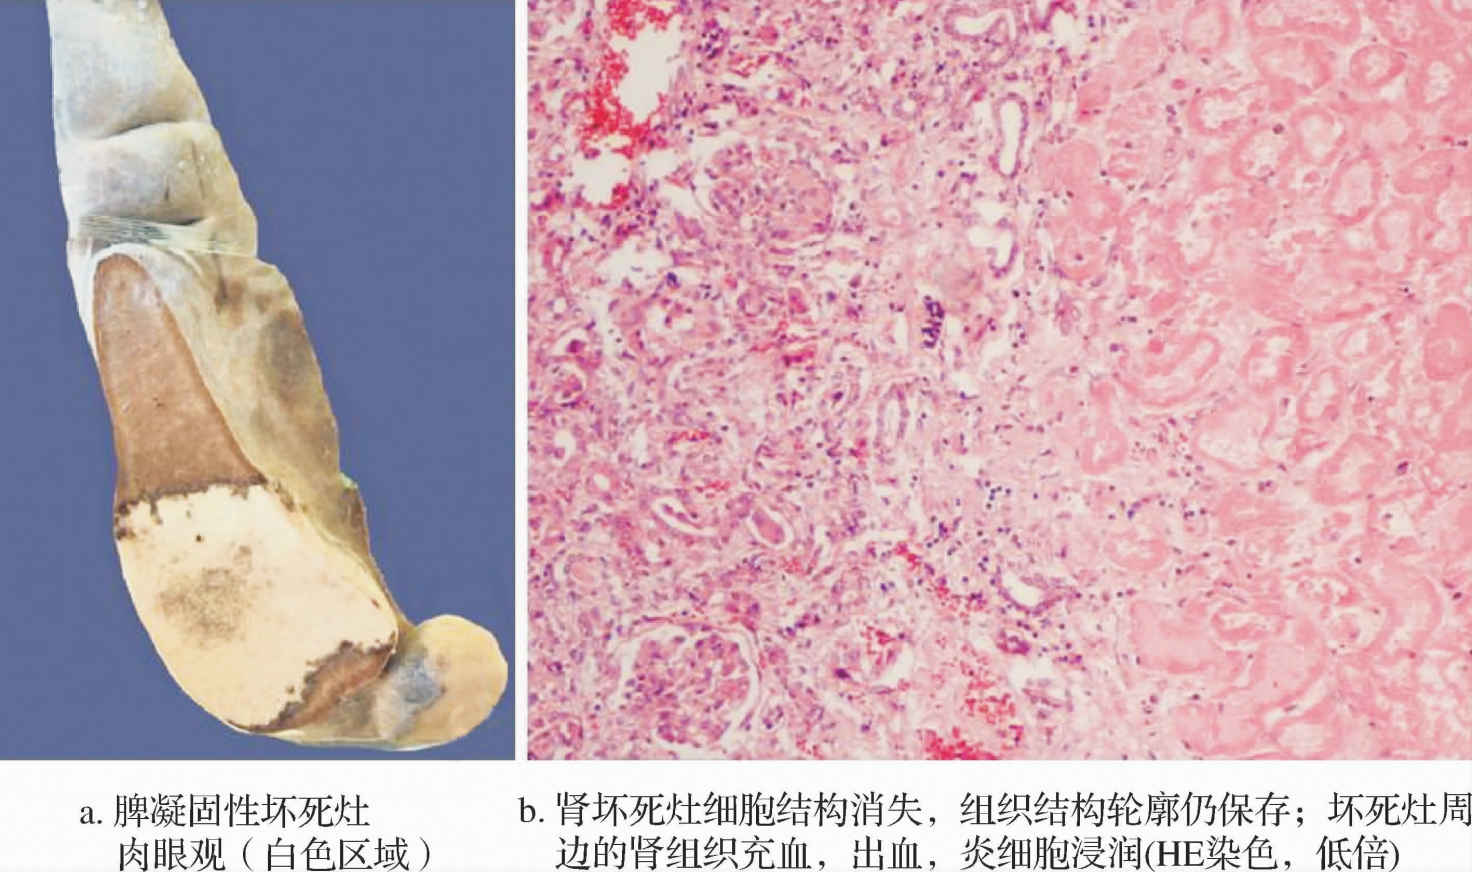
\includegraphics{./images/Image00015.jpg}
      \end{minipage}}\\
      \caption[]{}
  \end{figure}

  \begin{figure}
    \centering
    \subfloat[大脑半球外侧面的主要沟回]{
    \begin{minipage}[b]{0.7\textwidth}
      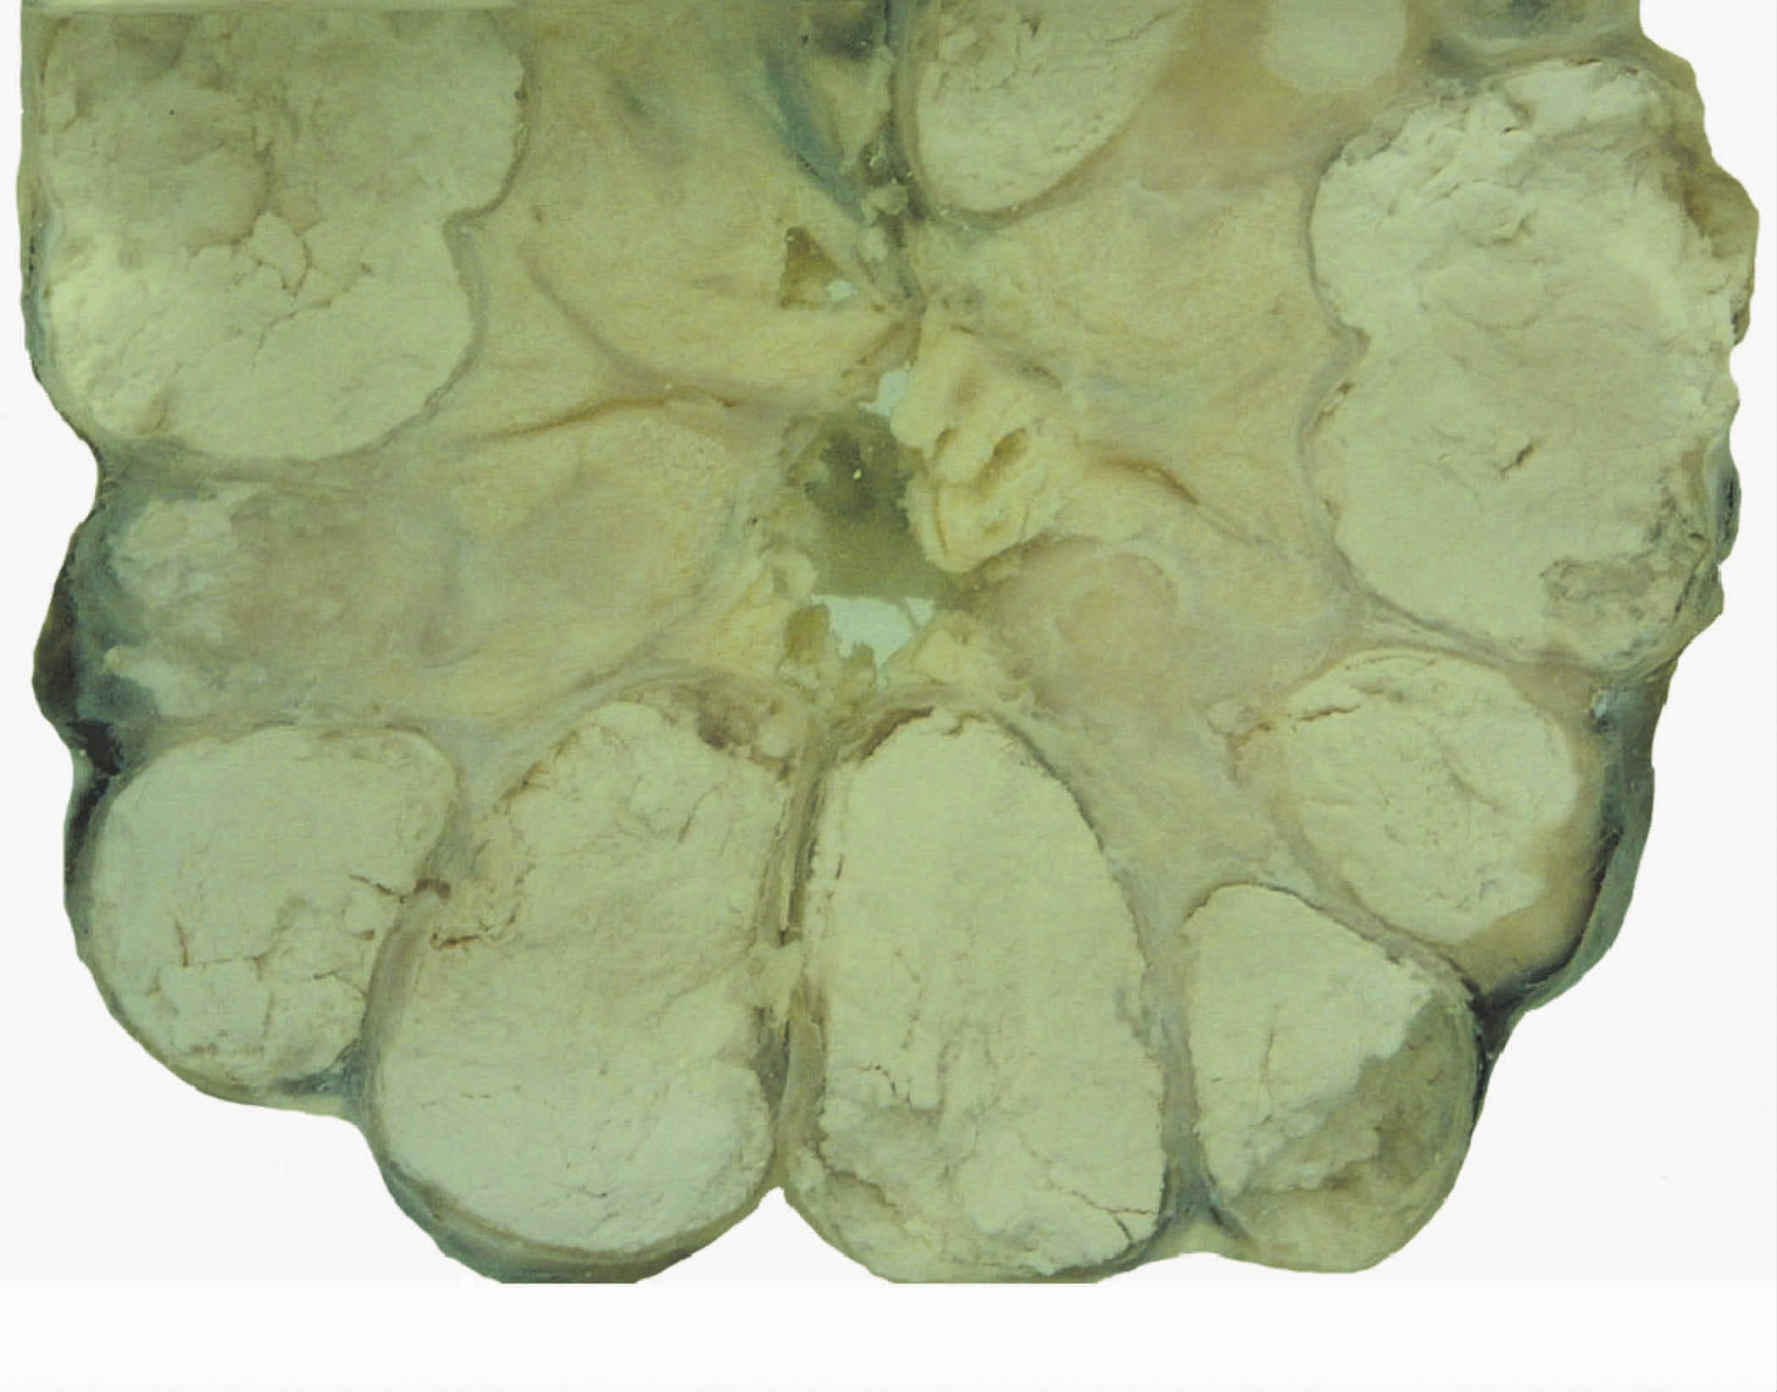
\includegraphics{./images/Image00016.jpg}
    \end{minipage}}\\
    \subfloat[大脑半球内侧面的主要结构]{
    \begin{minipage}[b]{0.7\textwidth}
      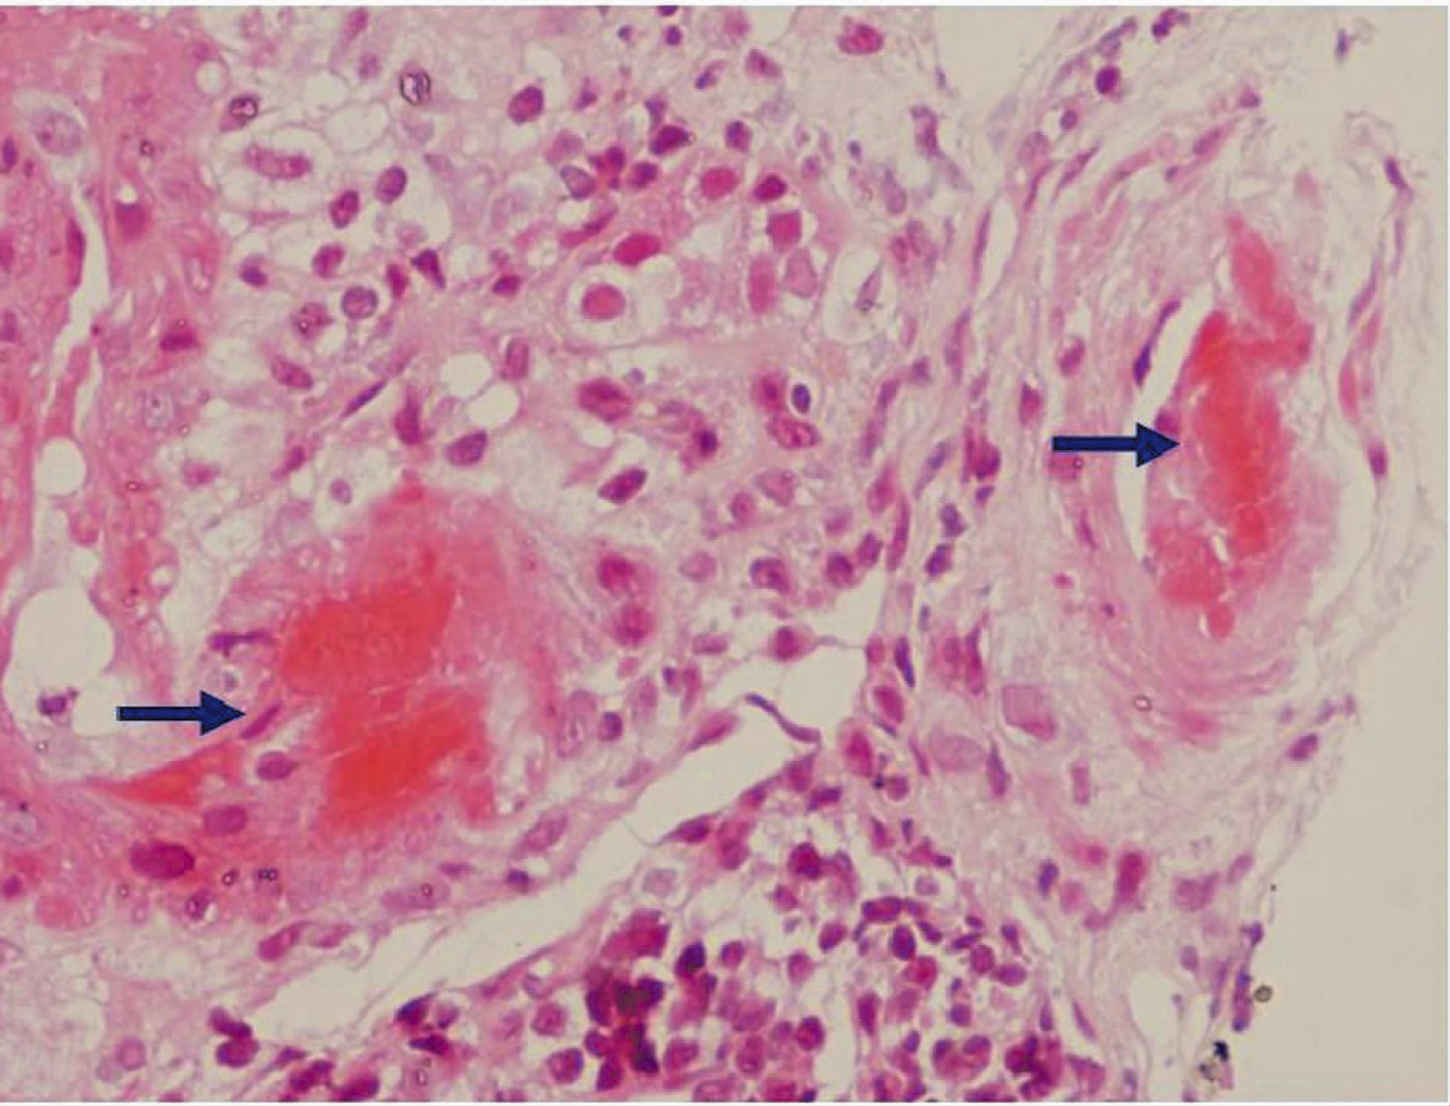
\includegraphics{./images/Image00017.jpg}
    \end{minipage}}\\
    \caption{}
    \label{fig2-4}
    \end{figure}

    \begin{figure}
      \ContinuedFloat             %%<-- put this in subsequest figures.
      \centering
      \subfloat[大脑半球背外侧面功能分区示意图]{
    \begin{minipage}[b]{0.7\textwidth}
      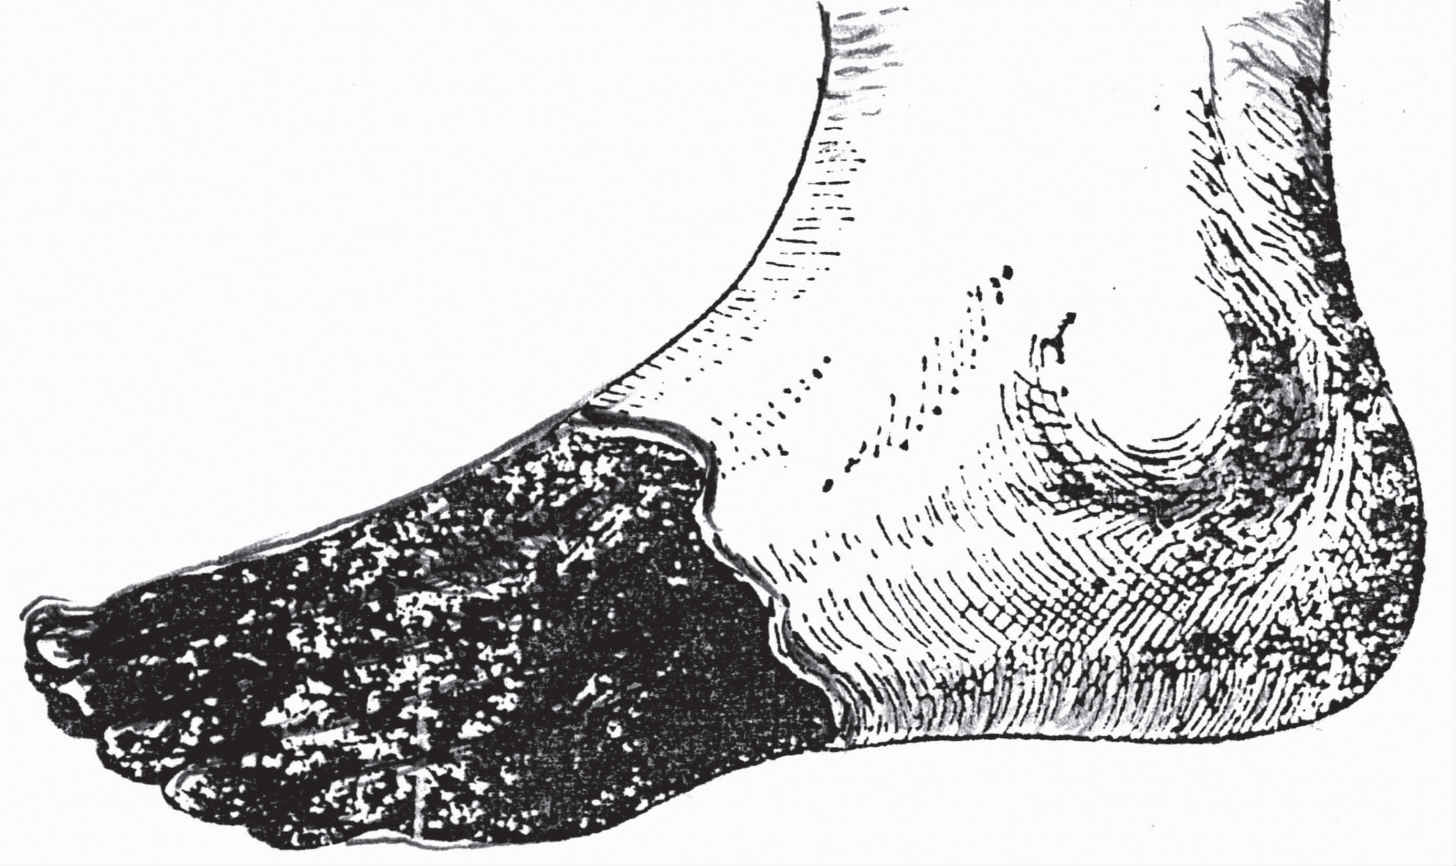
\includegraphics{./images/Image00018.jpg}
    \end{minipage}}\\
    \subfloat[大脑半球内侧面功能分区示意图]{
    \begin{minipage}[b]{0.7\textwidth}
      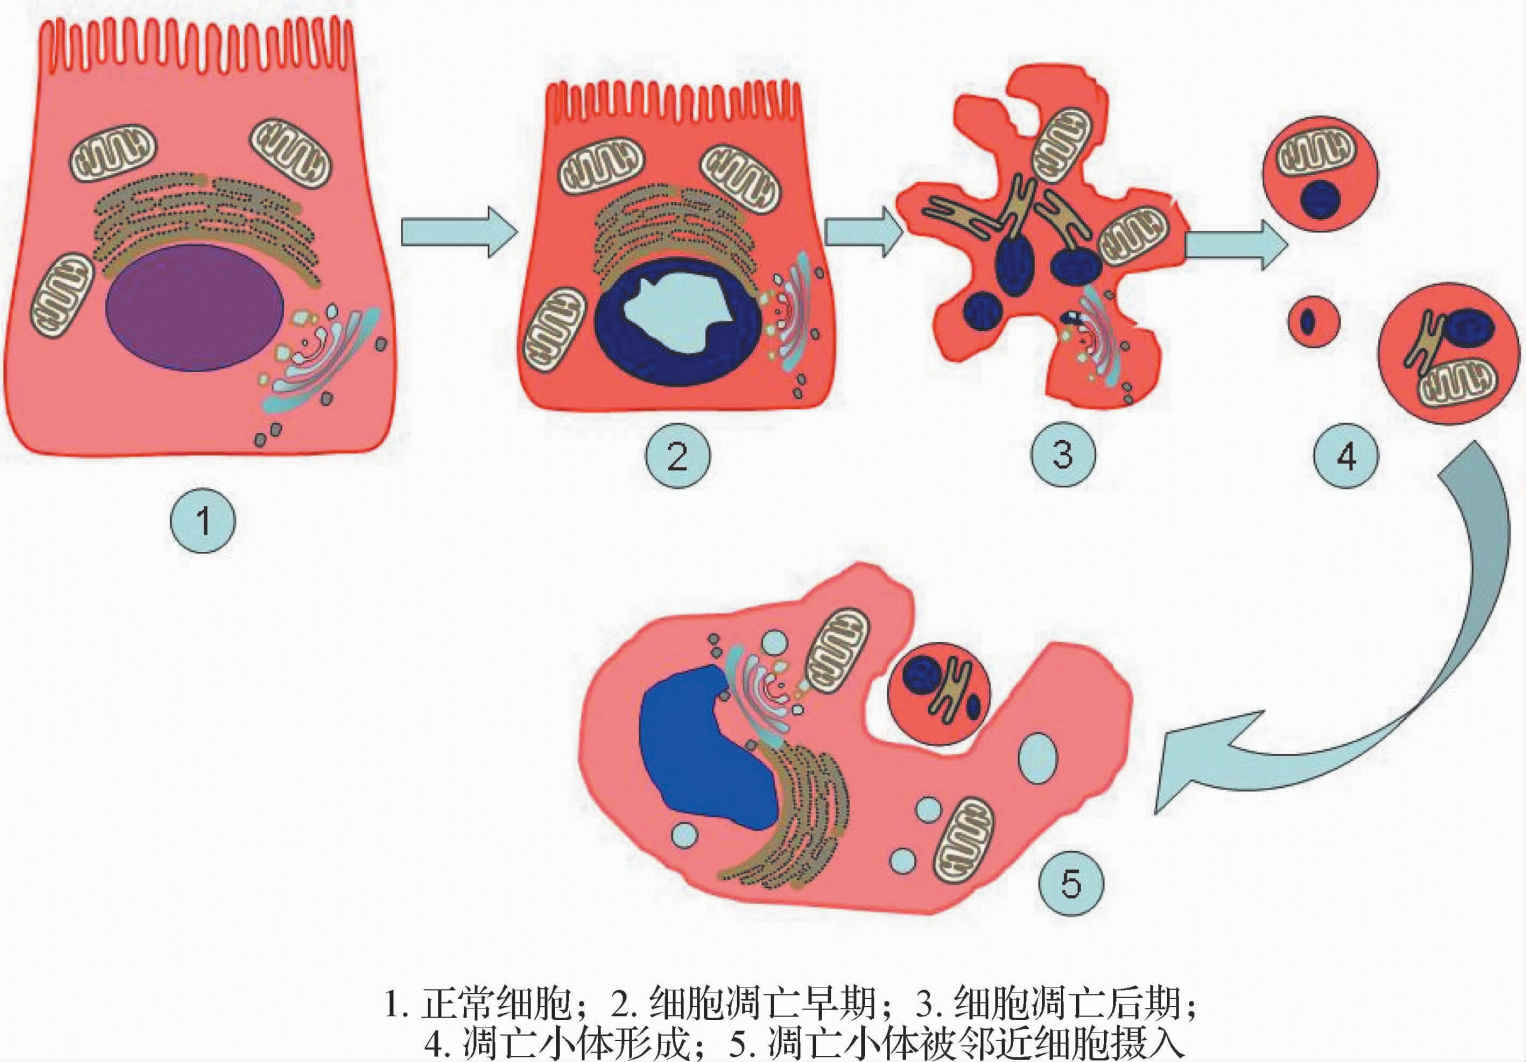
\includegraphics{./images/Image00019.jpg}
    \end{minipage}}\\
        \caption[]{}
    \end{figure}

\section{先天颅脑发育畸形和变异}

\subsection{概述}

所谓畸形是指胚胎期或胎儿期发生的脏器、系统或全身的形态异常或形成异常,不包括出生时的损伤和生后发育成长中产生的障碍。

先天性颅脑发育畸形的发病原因是由于胚胎期神经系统发育异常所致,约40%为遗传因素和子宫内环境的共同影响所致。前者包括染色体变异、显性或隐性遗传;后者包括宫内缺氧、感染等。其余60%病因复杂,机制不详。目前,可分为以下3大类:

1.器官形成障碍:①神经管闭合障碍:以脊髓脊膜膨出最常见,主要包括颅裂畸形(脑膜膨出、脑膨出、无脑畸形)、小脑扁桃体延髓联合畸形(Chiari畸形)、胼胝体发育不全、胼胝体脂肪瘤、先天性四脑室中侧孔闭锁(Dandy-Walker综合征)。②脑裂形成障碍:前脑无裂畸形(单叶、半叶、全叶)、视隔发育不良。③神经元移行异常:又称脑沟及细胞移行障碍,主要包括脑裂畸形、无脑回、灰质异常(巨脑回、多微脑回、灰质异位)。④大小异常:包括脑大、脑小畸形。⑤破坏性病变:包括积水性无脑畸形、脑穿通畸形。

神经管闭合不全是指胚胎期神经沟发育形成神经管的过程中,由于发育障碍而造成神经系统及其周围结构缺陷的一类中枢神经系统先天畸形,可能与孕妇叶酸缺乏有关。除表现出神经症状和体征外,更为常见的是周围组织的异常,包括颅骨、脑膜、椎体及其附件、皮肤和皮下组织(如先天性皮毛窦)等。该类疾病相当常见,其中尤以脊柱的畸形为多,是脑部的10倍或更多。

大脑皮层的神经元来自胚胎时期的脑室壁即神经管上皮。胚胎第6周末神经管经分化形成4个胚胎带,由内向外分别为脑室带、脑室下带、中间带和边缘带。脑室带和脑室下带的细胞具有分化成各类神经元的功能,故又称为生发基质层。胚胎7周时生发基质层的成神经细胞逐渐向外移行,大部分穿过中间带在边缘带内分化成神经元,形成有6层结构的正常脑皮质。26~30周脑回完全形成。神经元移行的过程复杂漫长,此间受到干扰则造成移行障碍。临床均以癫痫、智力障碍为最常见症状。

2.组织发生障碍:总体脑结构正常,但有异常细胞存在并持续分化。①神经皮肤综合征:包括神经纤维瘤病、脑颜面血管瘤病(Sturge-Weber综合征)、结节性硬化、视网膜小脑血管瘤病(又称Von
Hippel-Lindan病)。②血管性病变。③先天性肿瘤。

3.细胞发生障碍:①先天性代谢异常:包括氨基酸尿症、黏多糖沉积病、脂质沉积病等。②脑白质营养不良。③神经元变性。④轴索营养不良。

\subsection{脑膜膨出和脑膜脑膨出}

本病即显性颅裂畸形或称囊性颅裂畸形。临床可见颅外软组织肿物,大多于出生时即可发现。如仅有颅骨缺损,而无内容物自缺损处膨出称为隐性颅裂。

\textbf{【病理】}
颅裂多发生于中线或中线旁(斜坡除外),硬膜常缺如。脑膜(软膜和蛛网膜)或(和)脑突出于脑外,严重时可含部分脑室,可合并其他神经管闭合障碍(如Chiari畸形、胼胝体发育不全)等畸形。

\textbf{【临床表现】}
囊性肿物与头部相连,于出生时即可发现,也可于生后几个月或几年发现。哭闹或咳嗽时肿物增大,张力增加;压迫肿物,则前囟突出;局部可扪及骨缺损的边缘。一般无神经系统症状,也可表现为智力低下、抽搐及脑损害表现。

\textbf{【CT表现】}
软组织疝出的部位可见边缘硬化的颅骨缺损,枕部占70%,顶部占10%~20%,额上部占10%,颅底部占10%。应注意向颅外膨出的软组织,是否含有脑脊液和脑组织;颅底部膨出应注意与鼻息肉或鼻咽部肿瘤相鉴别(图\ref{fig2-5}\footnote{16岁女性,枕骨局限缺损,可见疝出之少量软组织密度灶})。同时,可合并胼胝体缺失、Chiari畸形、灰质异位等畸形。

\begin{figure}[!htbp]
 \centering
 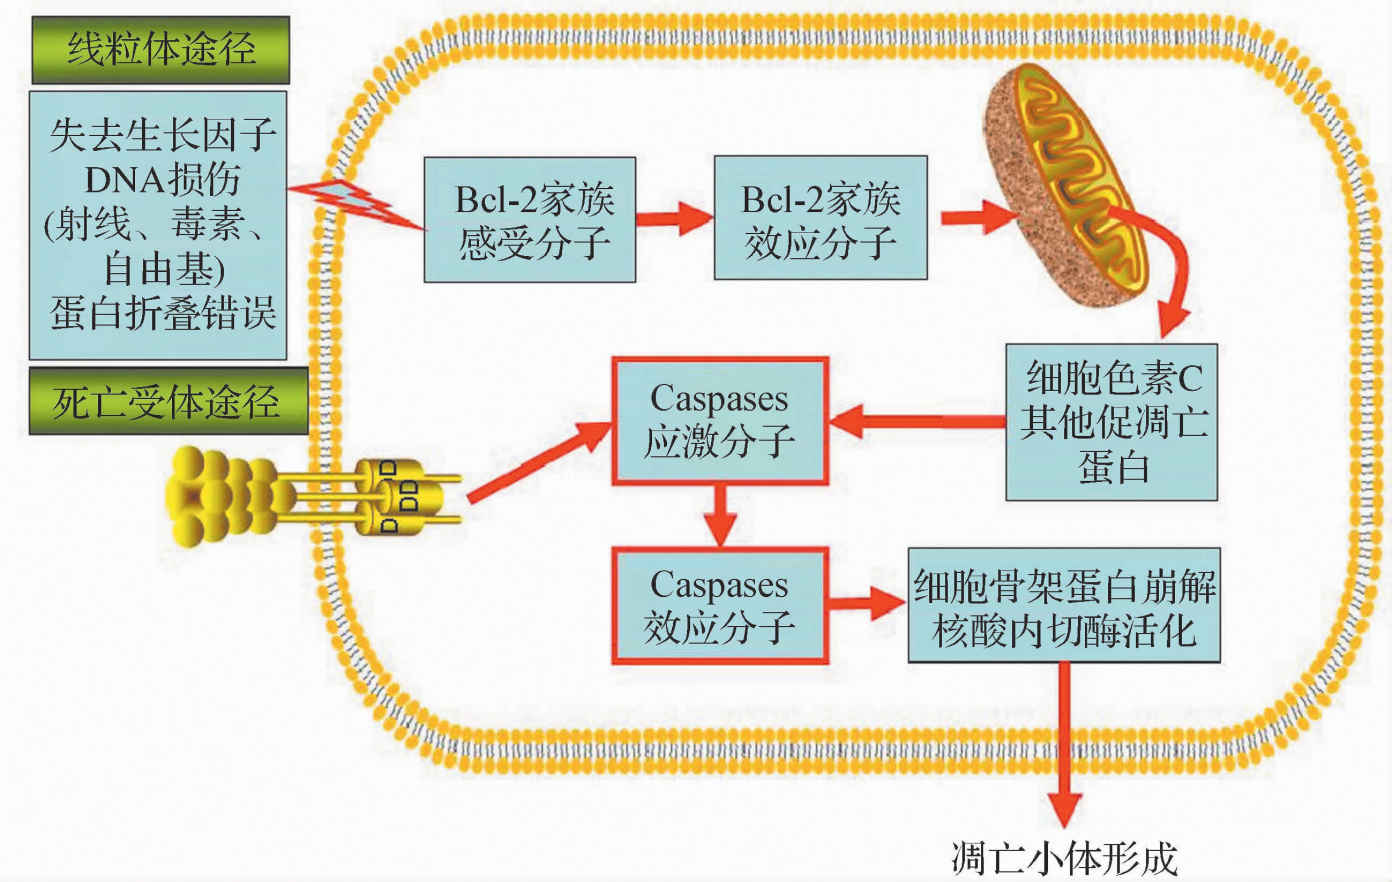
\includegraphics[width=.7\textwidth,height=\textheight,keepaspectratio]{./images/Image00020.jpg}
 \captionsetup{justification=centering}
 \caption{脑膜脑膨出}
 \label{fig2-5}
  \end{figure} 

\subsection{小脑扁桃体延髓联合畸形}

本病又称Chiari畸形,为后脑先天性发育异常。扁桃体过长、变形,经枕大孔疝入上段颈椎管,延髓和第四脑室可同时向下延伸。常伴脊髓空洞症、脊髓纵裂、脑积水和颅颈部畸形等。

\textbf{【病理】} 可分为以下4型。

Ⅰ型:多见。最可能的发病机制是胚胎枕节发育不良导致后颅窝狭小,难以容纳正常发育的后脑,使小脑扁桃体下疝。小脑扁桃体与小脑下部疝入颈椎管上端,无延髓移位。一般认为小脑扁桃体下端低于枕大孔≥5mm为下疝,<3mm为正常,二者之间临床意义不确定。通常不伴其他脑畸形,临床可无症状,或有轻度运动障碍和小脑症状。

Ⅱ型:最常见。小脑扁桃体和蚓部同时疝出枕大孔,脑桥下部及延髓下移,第四脑室延长。几乎总是伴有某种神经管闭合不全如脑膜膨出、脊髓脊膜膨出(腰骶部多见)、脑积水和脊髓空洞症。常有上述Ⅰ型症状。

Ⅲ型:十分罕见。为Ⅱ型伴有低枕部或高颈部脑膜脑膨出,临床症状较Ⅱ型更严重。

Ⅳ型:非常罕见。伴有严重的小脑发育不良,结构独特,可能不单独存在。该型归为小脑发育不良可能更合适。

\textbf{【临床表现】}
本病可无症状,尤其畸形轻者可无,也可直到成年甚至50~60岁始有症状。神经损害症状主要是颅神经和颈神经受损、延髓和上颈髓受压,可有小脑症状、颅内高压及脊髓空洞症表现。

\textbf{【CT表现】}
CT可显示下列特征:①小脑扁桃体、小脑蚓部及小脑、脑干和第四脑室下移;②脑积水;③大脑镰和天幕发育不良;④部分脑组织过度增生或脑发育异常导致脑室系统畸形;⑤后颅窝内容物的挤压引起的颅骨和蛛网膜下腔的改变。但只有通过脑池造影CT扫描或MR显示扁桃体下移、其下端变尖才能明确诊断。

\subsection{侧孔先天性闭锁}

本病又称Dandy-Walker综合征,第四脑室正中孔、外侧孔闭锁为发病主要原因。

\textbf{【病理】}
此病是一组先天性后脑发育畸形,包括脑积水、小脑发育障碍(小脑蚓部不发育或发育不全,约25%蚓部缺如)和与第四脑室相通的巨大后颅窝囊肿。囊肿大小变化很大,囊壁由下髓帆组成,包括室管膜、胶质、小脑组织、软脑膜和蛛网膜等,囊壁可钙化,可合并大脑发育异常。

\textbf{【临床表现】}
男女发病率相近。大多于2岁前产生症状,常因运动发育迟缓而就诊。部分因颅内高压或小脑症状而就诊,头颅明显增大。

\textbf{【CT表现】}
在出生时脑积水是不常见的,75%在生后3个月出现。典型者小脑蚓部体积变小或缺如,小脑半球分离;巨大的后颅窝“囊肿”与扩大的第四脑室相通。脑干前移,桥前池、桥小脑角池消失,后颅窝扩大,枕骨变薄,天幕上移。可合并胼胝体发育不良、多微脑回、灰质异位、枕部脑膨出等。

\textbf{【鉴别诊断】}
①后颅窝巨大蛛网膜囊肿:第四脑室与囊肿不相通,而是受压前移,必要时通过脑池造影CT鉴别。②巨大枕大池:第四脑室无受压,无蚓部发育不全、无后颅窝扩大等,但与下蚓部几乎完整的Dandy-Walker畸形不易鉴别。上述两者均可偶有轻度脑积水,但小脑发育基本正常。

\subsection{Joubert综合征}

\textbf{【病理】}
病理特征是小脑蚓部不发育或发育不全而形成异常的“中线裂”,还有小脑齿状核的变形、下橄榄核和旁橄榄核的发育不良、背侧柱核的异常以及锥体交叉缺如。

\textbf{【临床表现】}
男性多见,有发作性呼吸过度和(或)呼吸暂停、眼球活动异常(眼球震颤、斜视等)和儿童期发育迟缓。还可伴有其他异常如小头畸形、面部畸形、胼胝体发育不全、多指畸形和先心病等。

\textbf{【CT表现】}
在桥脑和中脑连接水平,第四脑室呈“蝙蝠翼状”。于第四脑室底部紧贴小脑半球中线处可见小脑半球间形成的切迹即“中线裂”。小脑上脚增粗,由于交叉的缺乏而向外分开,并导致中脑背侧局部缺失,形成所谓的“磨牙征”。第四脑室中部呈倒立三角形状,与不连接的小脑半球间的脑脊液间隙相连形成“酒杯状”表现,无后颅窝囊肿和脑积水。

\subsection{胼胝体发育不全}

\textbf{【病因病理】}
胼胝体在妊娠12~20周时形成。本畸形偶然发病,病因一般不明,多为先天性。在某些病例中,母体的血管性、外伤性、中毒性或感染性损伤为致病因素。产期缺血缺氧性损害也可引起获得性胼胝体发育不全。本病可为全部或部分缺如,常伴发其他畸形(最高达50%),如前脑无裂畸形、多微脑回、厚脑回、灰质异位、脑小畸形、视隔发育不良、胼胝体脂肪瘤或纵裂池蛛网膜囊肿等。

\textbf{【临床表现】}
临床症状各不相同,视伴发的其他神经系统畸形而定。许多患者可无症状或仅有轻度视觉障碍;或有交叉触觉定位障碍而智力正常;严重者可有癫痫和智力不全。

\textbf{【CT表现】}
由于胼胝体完全或部分缺如而表现不一。可见纵裂池前部明显向后伸展,靠近第三脑室前壁。侧脑室额角和体部间距增大,而且两侧脑室平行分离,并可见其内壁呈弓形外突,冠扫额角呈“八”字形分离。枕角不对称性扩大(憩室),第三脑室轻度扩大并上移。正常时,两侧脑室的脉络丛常在室间孔间会聚,并形成45\textsuperscript{o}
~70\textsuperscript{o} 夹角,本病此夹角多<35\textsuperscript{o}
~40\textsuperscript{o}
(图\ref{fig2-6}\footnote{A~D为同一患者,可见纵裂池前部明显向后伸展,靠近第三脑室前壁;第三脑室轻度扩大并上移;侧脑室额角和体部间距增大,两侧脑室平行分离}),有时可见半球间裂(纵裂池)的蛛网膜囊肿等畸形。本病应注意与脑室周围白质软化症(PVL)相鉴别。



\begin{figure}[!htbp]
 \centering
 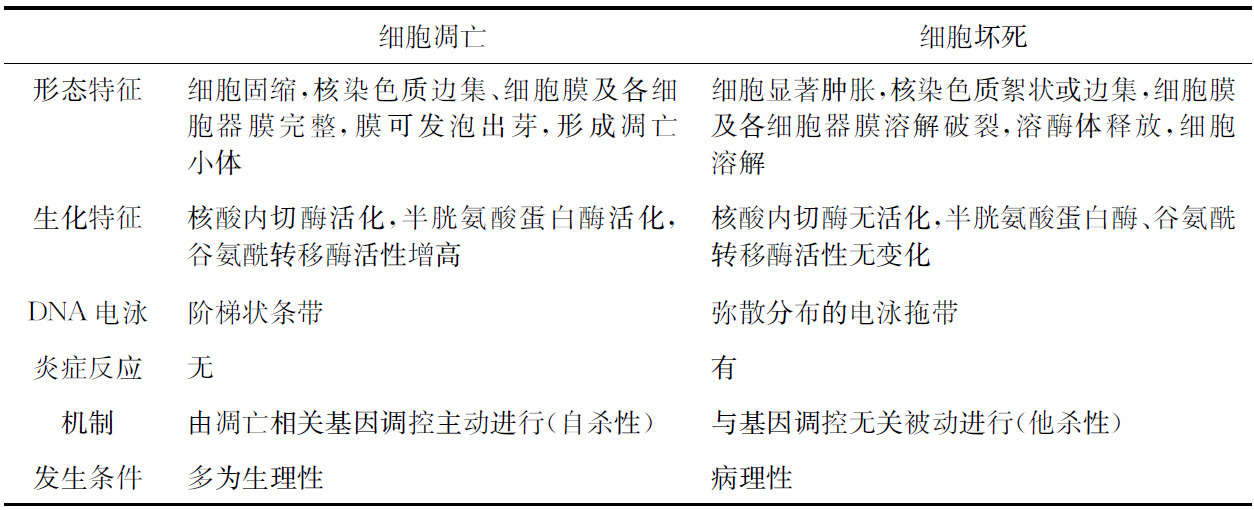
\includegraphics[width=\textwidth,height=\textheight,keepaspectratio]{./images/Image00021.jpg}
 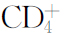
\includegraphics[width=\textwidth,height=\textheight,keepaspectratio]{./images/Image00022.jpg}
 \captionsetup{justification=centering}
 \caption{胼胝体发育不全}
 \label{fig2-6}
  \end{figure} 


\subsection{前脑无裂畸形}

本病又称全前脑畸形,是胚胎发育过程中由前脑发育障碍引起的一组复杂的颅脑与面部畸形。

\textbf{【病因病理】}
其病因不明,部分为常染色显性和隐性遗传。大脑不能分裂成两侧大脑半球,有时也不能在横向上分裂成端脑和间脑,可分为无脑叶型、半脑叶型、脑叶型3种类型,代表了畸形的不同程度。

\textbf{【临床表现】}
男女发病相近,因婴儿多数死于流产或出生后不久,故临床少见。脑叶型可活到成年,并有运动迟缓、智力低下等神经精神症状。

\textbf{【CT表现】} 3种类型分别表现如下。

1.无脑叶型:又称全前脑无裂畸形。脑呈小圆球形,丘脑融合,中央单脑室,第三脑室成为扩大脑室的一部分。正常中线结构如透明隔、大脑镰、胼胝体和纵裂均缺失,50%以上有多处面颅畸形。

2.半脑叶型:中央单脑室较小,初步形成了额、枕角,胼胝体、大脑镰、透明隔仍缺如。大脑半球前部仍保持融合,但后部半球间裂已形成。丘脑往往部分分离,故第三脑室是小的,面部畸形不重。

3.脑叶型:CT表现比前两者轻微。前部半球间裂较浅,仍存在融合表现。脑室系统形态良好,透明隔缺如。脑镰和胼胝体至少部分形成,丘脑无融合。

此外,少数病例额部和枕部半球间裂均存在,融合发生于半球额后顶区域,属半脑叶型,CT诊断困难。

\subsection{视隔发育不良}

本病罕见,主要是透明隔发育不全,常见于先天性垂体性侏儒,可能是脑叶型前脑无裂畸形的轻度形式。

\textbf{【病理】}
透明隔发育不全,有原始的视泡及视交叉、视神经,漏斗发育不全而使视神经孔狭小。

\textbf{【临床表现】}
眼部症状包括眼球震颤和视敏度下降,但可有正常视力。约2/3有下丘脑-垂体功能障碍而出现尿崩、生长发育障碍。

\textbf{【CT表现】}
透明隔缺如,额角在横断面呈倒三角形或盒状。严重者可见视神经、视交叉细小,视神经管小和视交叉位置异常,视交叉和下丘脑发育不全使鞍上池扩大。

\subsection{透明隔疾病}

透明隔是一厚约1.5~3.0mm的双层半透明膜,上起胼胝体的体部、膝部和嘴部,向下延伸至穹隆的表面,前后伸延从终板、胼胝体的嘴至胼胝体的压部。它含有一定数量的胶质细胞、散在的神经元和神经纤维。这些神经纤维构成了海马和下丘脑之间的重要联系,且是中继下丘脑到海马、杏仁核、缰核和脑干网状结构的内脏信息的相关中心及边缘系统到脑干网状结构的重要环路。所以,它参与意识、睡眠以及环境作用所表现出来的情绪反应,例如饮食、性活动等,并有助于精神活动的自我平衡。

透明隔疾病有:①透明隔间腔:即第五脑室。②透明隔缺如:原发或继发。③透明隔囊肿:与第五脑室并无严格界限,表现囊壁向两侧突出而不是平行,宽达10mm以上,并可引起室间孔狭窄导致脑积水,邻近神经组织受压而引起神经功能障碍。当宽径<5mm时,则不引起症状(图\ref{fig2-7})。④肿瘤:罕见,如星形细胞瘤、少突胶质细胞瘤、室管膜瘤和成星形细胞瘤,近来亦有亚室管膜瘤、局限性脂肪瘤的报道。⑤血管瘤。⑥钙化。⑦移位。⑧萎缩。

\begin{figure}[!htbp]
 \centering
 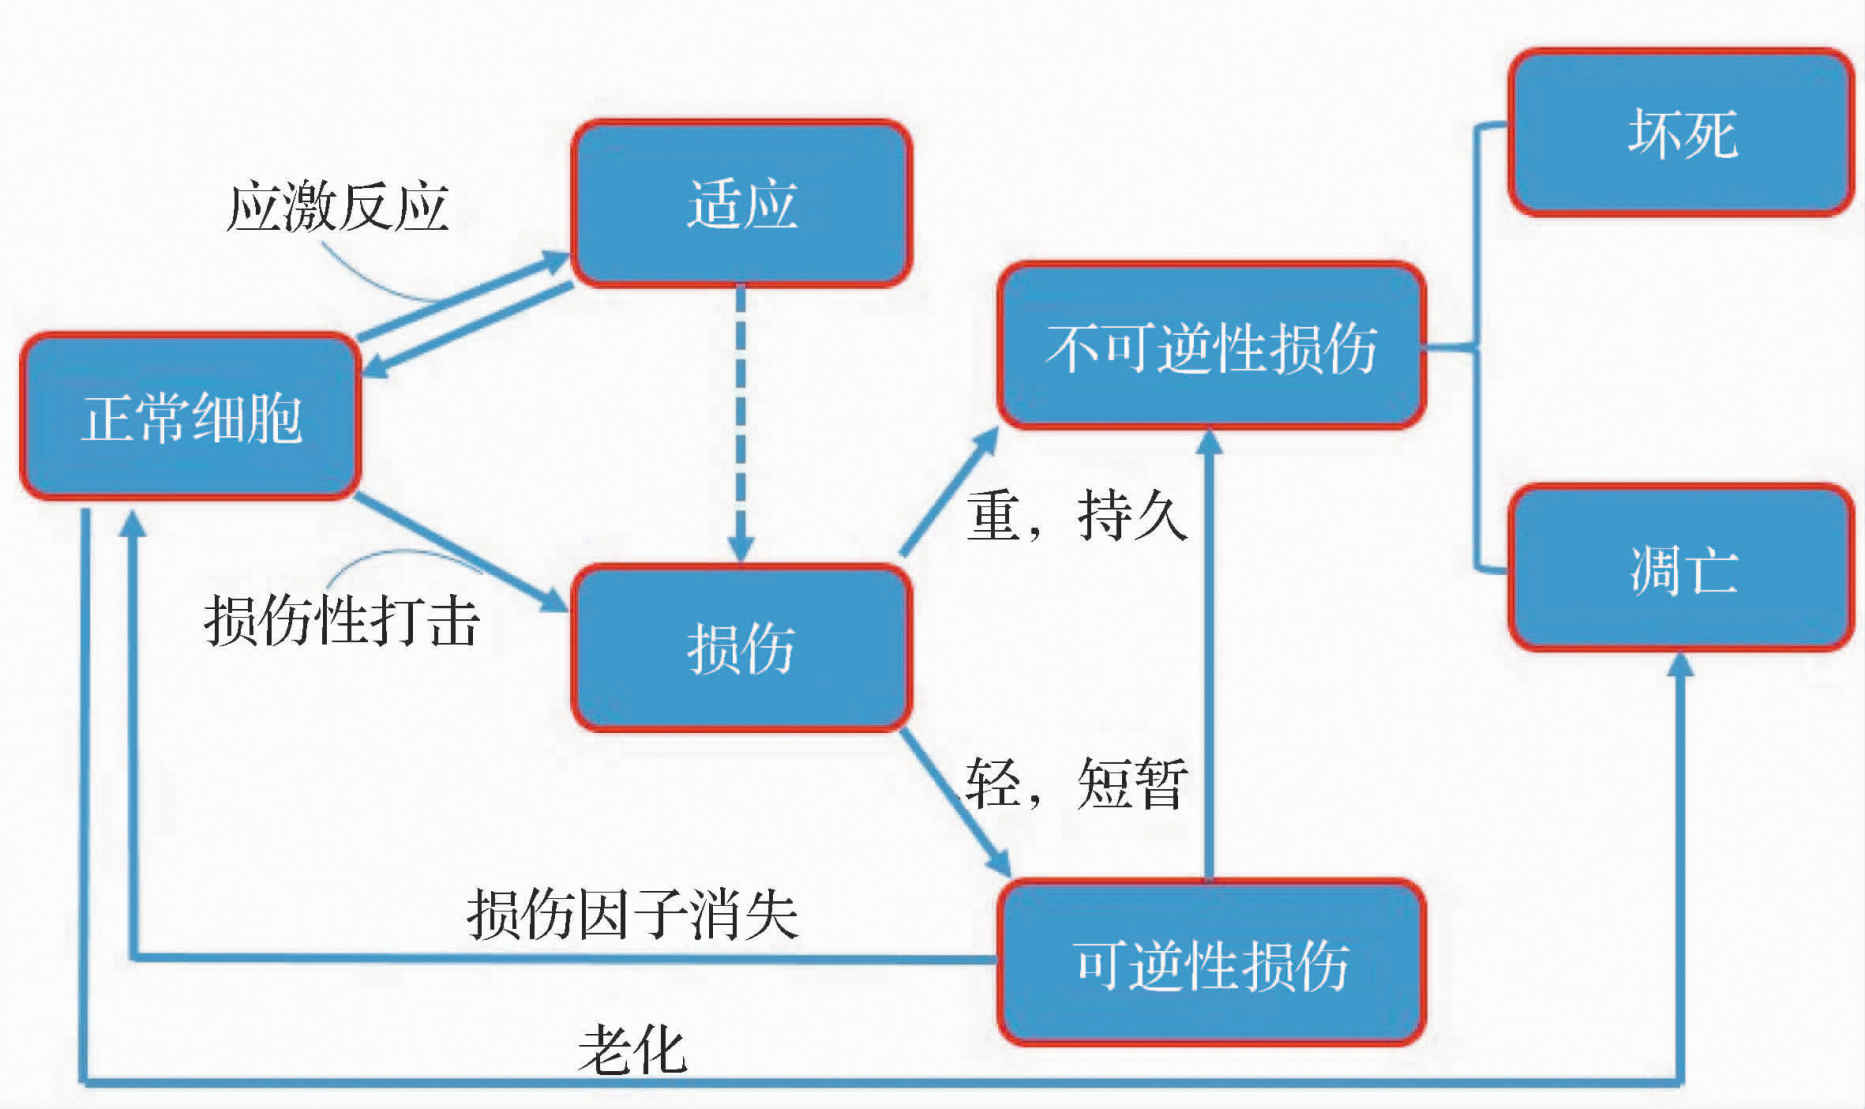
\includegraphics[width=.7\textwidth,height=\textheight,keepaspectratio]{./images/Image00023.jpg}
 \captionsetup{justification=centering}
 \caption{透明隔囊肿\\{\small 透明隔区囊状水样密度灶,囊壁向两侧突出,宽达12mm}}
 \label{fig2-7}
  \end{figure} 



\subsection{侧脑室黏合}

侧脑室不对称在正常人中常见,部分原因是侧脑室黏合,侧脑室黏合是正常变异。

\textbf{【病理】}
本症是在生长发育过程中侧脑室内面部分融合,造成侧脑室不对称、变形。发生在胎儿期4~6周,此时脑白质发育迅速,白质膨大可使邻近的室管膜表面挤压在一起。黏合多发生在额角上侧面及体部,单侧或双侧性。

\textbf{【CT表现】}
侧脑室黏合可以是单侧性或双侧性,或与透明隔间腔同时存在。额角的前部融合,致额角前部消失,额角变短,两壁夹角为锐角,使两壁相交处圆钝的正常表现消失,透明间隔居中。额角中部的两壁尖角状突起,中部间隙消失或接近消失,透明隔居中。透明隔移向一侧,偏移程度从轻度到非常明显,致同侧侧脑室体部变小,对侧相对增大。透明隔的移位必然伴有体部变小侧的额角变窄、变形,但透明隔始终呈直线状走行。双侧基底节区形态结构对称,脑室、脑实质内无异常,增强扫描无异常强化。

\subsection{脑裂畸形}

\textbf{【病因病理】}
有学者认为,妊娠第2个月出现的病理干扰可造成脑壁某部位生发基质层不能正常发育,致使神经元移行不能发生或过早停下来而导致脑裂畸形。其主要病理改变为大脑半球内有自脑表面向内延伸达室管膜下的横行裂隙,邻近皮层卷入衬于裂隙两侧,其表面的软脑膜与室管膜融合形成软脑膜-室管膜缝。脑裂畸形可分为闭合型和分离型两型,常合并透明隔缺如、胼胝体发育不良及其他神经元移行异常等畸形。

\textbf{【临床表现】} 主要有癫痫、智力低下和运动功能障碍。

\textbf{【CT表现】}
大脑半球表面有单侧或两侧的裂隙,从脑表面延伸到室管膜下区。脑皮质沿裂隙内折,居裂隙两侧,多位于中央前后回附近。根据其表现可分为两型:①Ⅰ型:即融合型(或称闭唇型)脑裂畸形,裂隙关闭不与侧脑室相通,但脑室壁可有憩室样突起(图\ref{fig2-8});②Ⅱ型:即分离型(或称开唇型)脑裂畸形,特点为内折的皮质分离,形成较大裂隙并多与侧脑室相通,且脑室壁在内压作用下外突,形成憩室。

\textbf{【鉴别诊断】}
①脑穿通畸形:为大脑成形后的损害(坏死腔),多呈圆形,无脑皮质沿囊肿壁内折为鉴别要点。有时鉴别困难,但穿通畸形的两缘向病灶外方突出,而分离型脑裂畸形两缘向内突出有助于鉴别。②孤立性灰质异位:当融合型裂隙不明显时应注意与其鉴别。脑裂畸形皮质柱内端相邻的侧脑室外壁常有憩室状突起,外端脑表面有楔形凹痕,可与其相鉴别。

\subsection{多微脑回畸形和鹅卵石样脑回畸形}

\subsubsection{无脑回}

大脑皮质表面光滑、无沟回,故又称光滑脑。灰质增厚,白质变薄,灰白质正常手指样交界消失,也可与巨脑回相伴发。

\subsubsection{巨脑回}

局限性或弥漫性脑回异常增宽,皱褶减少,表现为宽、平、厚的脑回,灰白质正常手指样交界亦可消失(图\ref{fig2-8},图\ref{fig2-9})。

\begin{figure}[!htbp]
 {\centering
 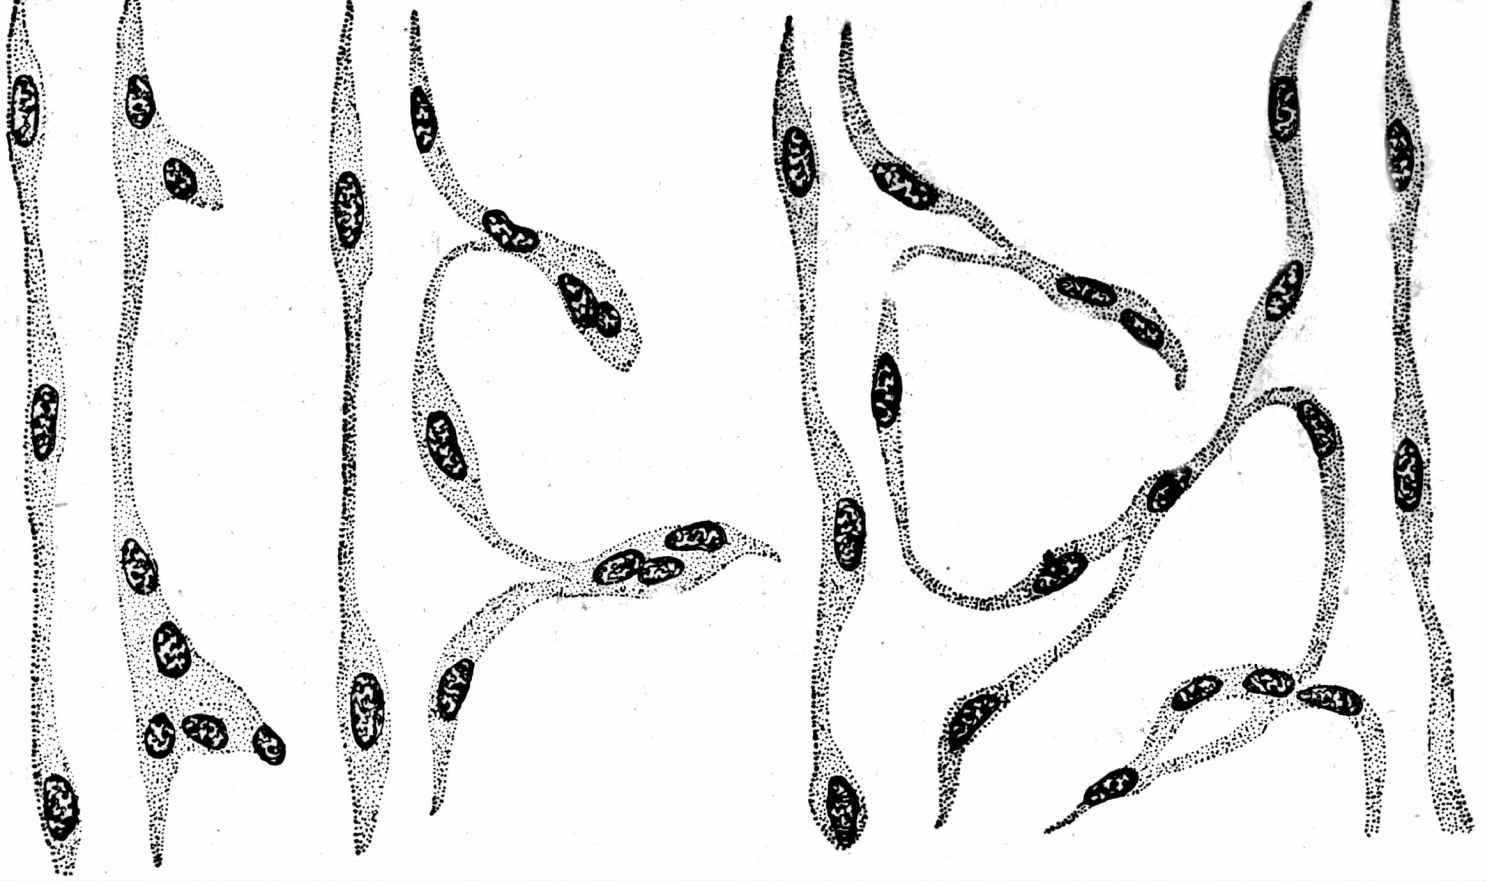
\includegraphics[width=.7\textwidth,height=\textheight,keepaspectratio]{./images/Image00024.jpg}
 \captionsetup{justification=centering}
 \caption{脑裂畸形、双侧额叶巨脑回\\{\small  A、B为同一患者,大脑半球表面两侧均有裂隙,脑皮质沿裂隙内折,位于裂隙两侧,裂隙关闭不与侧脑室相通,灰质相应内移,双侧额叶巨脑回}}
 \label{fig2-8}}
  \end{figure} 



\begin{figure}[!htbp]
 {\centering
 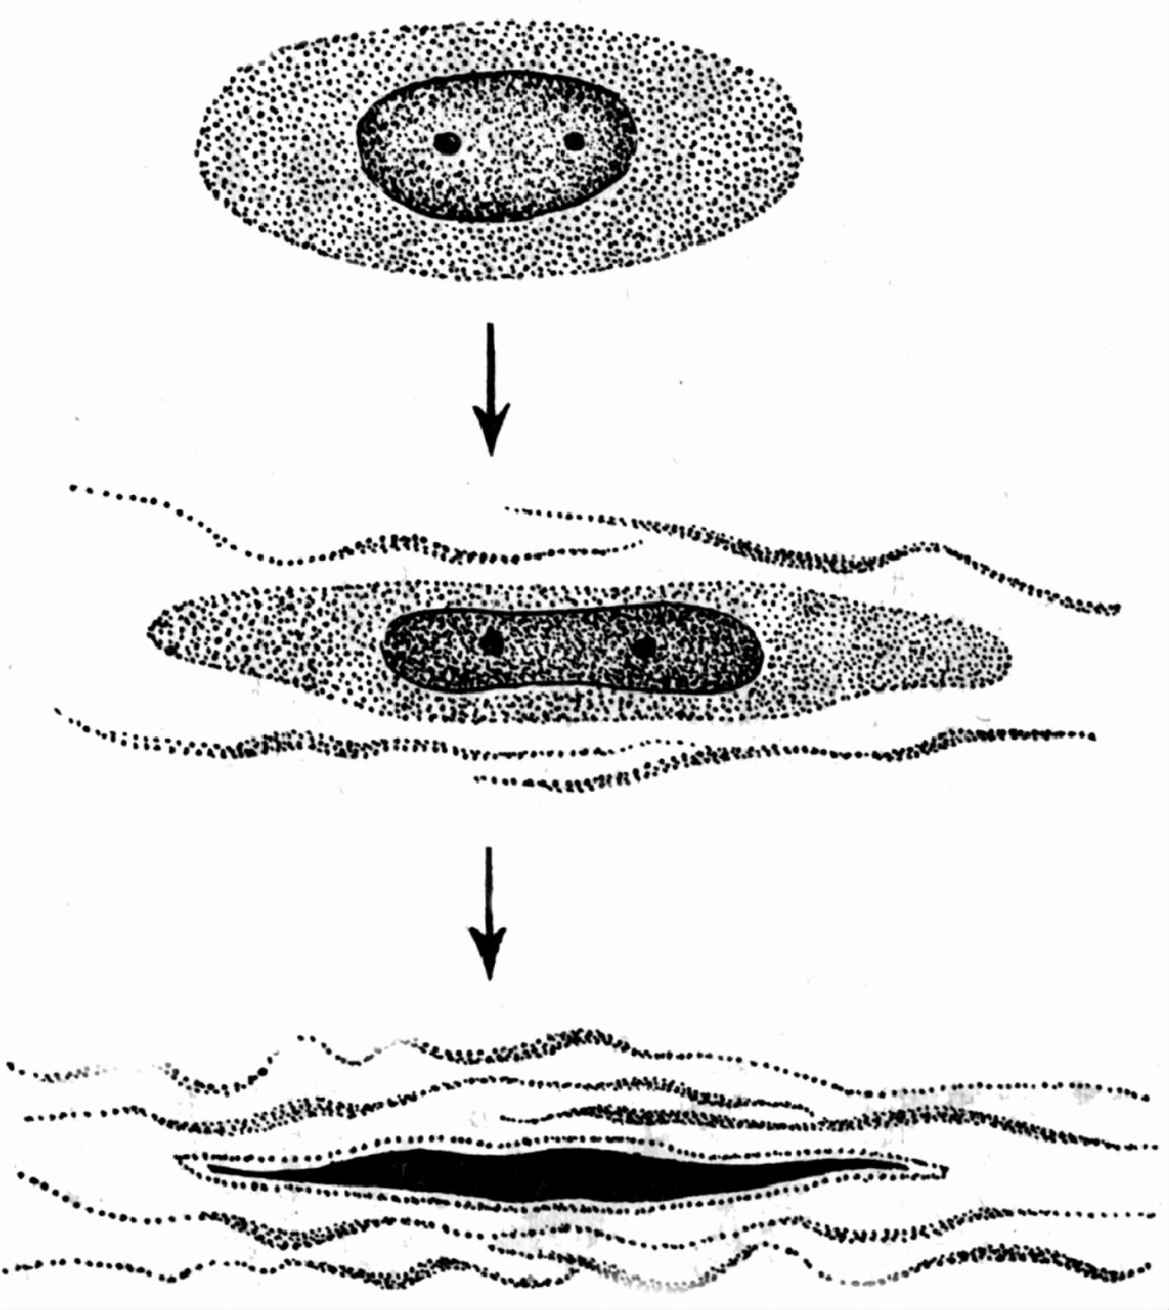
\includegraphics[width=.7\textwidth,height=\textheight,keepaspectratio]{./images/Image00025.jpg}
 \captionsetup{justification=centering}
 \caption{巨脑回}
 \label{fig2-9}}

 右侧额、顶叶脑回弥漫性异常增宽,皱褶减少
  \end{figure} 



\subsubsection{多微脑回畸形}

亦称多小脑回畸形(但该名称易与小脑病变混淆),脑回小且数目增多。

\subsubsection{鹅卵石样脑回畸形}

为复杂的脑畸形,包括鹅卵石样皮质、白质异常、脑室扩大,及脑干、小脑变小并伴有小脑的多微脑回。皮质的异常为无脑回、巨脑回和多微脑回的混合。

\subsection{灰质异位}

本病为灰质在异常部位的聚集。

\textbf{【病因病理】}
原因不明,可能与遗传性、血管性、感染性、环境因素(中毒、辐射、胎儿酒精综合征等)等有关。病理上根据异位灰质灶是否与室管膜相连分为室管膜下型和非室管膜下型,根据病变范围又可分为局灶性和弥漫性。弥漫性90%为女性,往往具有家族史。本病还可伴有其他畸形。

\textbf{【临床表现】}
单纯的灰质异位预后好,可无症状或仅有癫痫。病灶较大或同时伴有其他畸形可表现为中度或严重发育延迟、偏瘫伴癫痫。

\textbf{【CT表现】}
白质内有与灰质密度相等的异常影,增强扫描密度与灰质一致。本病有多种分型方法,通常可分为以下3型。①结节型:呈结节状分布于侧脑室旁,并可突向脑室。②板层型:不规则分布于白质内。③带状型:呈带状分布于白质或皮层下(是最严重的类型,常伴有难治性癫痫,预后相对差)。前两型可单发或多发、单侧或双侧,灰质结节直径1~30mm,无水肿和占位效应。带状型多分布对称,且表面脑回多正常,故较难分辨,易漏诊。

\subsection{脑大畸形}

本病又称头大畸形、巨脑症,为先天性大脑皮质增厚及神经胶质细胞增生。

\textbf{【病因病理】}
本病病因不明,可与遗传因素有关。有学者认为包括体积过大和质量过重两种情况,并将它分为解剖型和代谢型巨脑症。解剖型指细胞体积或数目大于正常,可伴软骨发育不全、神经纤维瘤病、结节性硬化和Chiari畸形等。代谢型是指异常代谢产物积蓄致脑细胞增大,部分伴白质发育不良。本病出生时脑重即可达1600g,或生后头颅迅速增大,皮质和髓质均增厚,可有髓鞘形成不良,无脑积水。

\textbf{【临床表现】}
儿童期发病,常有癫痫和智能低下。头颅周径增大,似先天性脑积水,但无眼球下斜征象(落日征),常有视、听力障碍。

\textbf{【CT表现】}
头颅和颅腔明显增大,大脑皮质增厚,但脑组织密度正常。脑室正常或轻度扩大,脑沟、池正常,中线结构居中。前囟较大、闭合延迟,颅板较薄。

\textbf{【鉴别诊断】}
应注意与继发性巨脑症(如较弥漫的肿瘤、结节性硬化、海绵状硬化及脑积水)、单侧巨脑畸形相鉴别。

\subsection{脑小畸形}

本病又称小脑症、小头畸形或脑小症,发病率为2.5/10万。

\textbf{【病因病理】}
病因不明,可包括先天性遗传因素和胎儿期、新生儿期的各种致病因素如感染、出血、缺氧、产伤等。病理表现为脑小,重量为正常的1/4~1/3,并且脑回结构简单,皮质发育不全,神经元数目减少、排列不整齐,颅骨和颅腔发育小,可合并其他脑发育畸形。

\textbf{【临床表现】}
常表现智能低下甚至呈白痴,也可合并癫痫、运动功能障碍等,出生时头小、外形特殊。

\textbf{【CT表现】}
轻度者可无阳性表现,病变明显时脑室系统和蛛网膜下腔可扩大,皮质光滑,缺乏脑沟、回。严重者可合并胼胝体发育不全、透明隔发育异常、穿通畸形等。颅腔缩小以额部明显,颅板较厚,板障增宽,内板平坦光滑。

\textbf{【鉴别诊断】}
狭颅畸形是颅缝过早闭合限制了脑的发育所致。颅腔常有变形,颅骨脑回压迹增多,且脑室、脑沟、脑池及脑实质常无明显异常,不难与脑小畸形鉴别。此外,一侧大脑半球发育不全与脑小畸形病因病理一样,临床和CT表现相近,不难诊断和鉴别。

\subsection{积水型无脑畸形}

本病是一组少见的先天性前脑畸形,见于婴幼儿,发生率新生儿中占0.2%左右。

\textbf{【病因病理】}
可能与胚胎期脑供血障碍有关,也有人认为是全脑穿通畸形。主要病理改变为双侧大脑半球的额、顶、颞叶完全或大部分缺如,由充满脑脊液的囊性区域取代,其内衬由软脑膜构成(不含室管膜)。基底节、丘脑、中脑可部分或大部分破坏,小脑、桥脑、延髓可发育正常或畸形,脑室系统偶可保存完好,脑膜正常存在,颅骨颅腔大小形态正常或增大。

\textbf{【临床表现】}
头围逐渐增大,多智力低下,可有眼球不规则运动、眼落日征,以及肌张力高、腱反射亢进、抽搐或惊厥、运动机能障碍等。

\textbf{【CT表现】}
幕上双侧大脑半球、脑室大部分缺失,整个颅腔大部分呈脑脊液密度。仅于脑底部见残存的部分枕、额或(和)颞叶组织,基底节、丘脑部分存在,大脑镰完整存在。幕下结构正常,但脑干可略变细。

\textbf{【鉴别诊断】}
有学者把极其严重的双侧性开唇型脑裂畸形归类于积水性无脑畸形中,影像学二者难以鉴别,但后者还能识别脑室轮廓,特别是前角的下部和后角。还应注意与无脑叶型前脑无裂畸形、穿通畸形、巨大蛛网膜囊肿及重度脑积水鉴别。

\subsection{脑穿通畸形}

本病是在脑组织分化发育充分之后,由于各种原因造成的脑组织破坏缺损,并与蛛网膜下腔或脑室相通。

\textbf{【病因病理】}
有先天性和获得性之分。先天性病因不明,可能与胎儿期血管闭塞或发育畸形有关;获得性是由于外伤、感染、缺氧、血管疾病引起正常脑组织坏死液化。缺损边缘为胶质瘢痕,不含神经细胞。

\textbf{【临床表现】} 依病变范围而定,可表现运动障碍、癫痫等。

\textbf{【CT表现】}
脑实质内巨大的脑脊液密度样囊肿,界限清楚,增强扫描无强化。与脑室或(和)蛛网膜下腔相通是诊断的关键,同侧侧脑室一般相应扩大。

\subsection{先天性中脑导水管狭窄}

本病亦属脑的发育畸形。

\textbf{【病理】}
狭窄多位于导水管口以下3~4mm处。狭窄的形态多样,可呈线状、鸟嘴状、漏斗状、隔膜状或分叉状,狭窄以上脑室积水。

\textbf{【临床表现】} 临床症状常开始于幼儿,呈慢性脑积水表现。

\textbf{【CT表现】}
侧脑室及第三脑室对称性扩大,第四脑室正常或略小。侧脑室周围有带状低密度区,代表阻塞性脑积水的典型表现。重度积水患者,可表现幕上大脑半球区为水样低密度,额、顶、颞叶脑实质几乎消失或残留极少,部分枕叶、基底核和丘脑保存,小脑和脑干发育一般正常,第四脑室位置、形态正常,可见正常大脑镰结构(图\ref{fig2-10}),MR可显示狭窄的形态。

\begin{figure}[!htbp]
 {\centering
 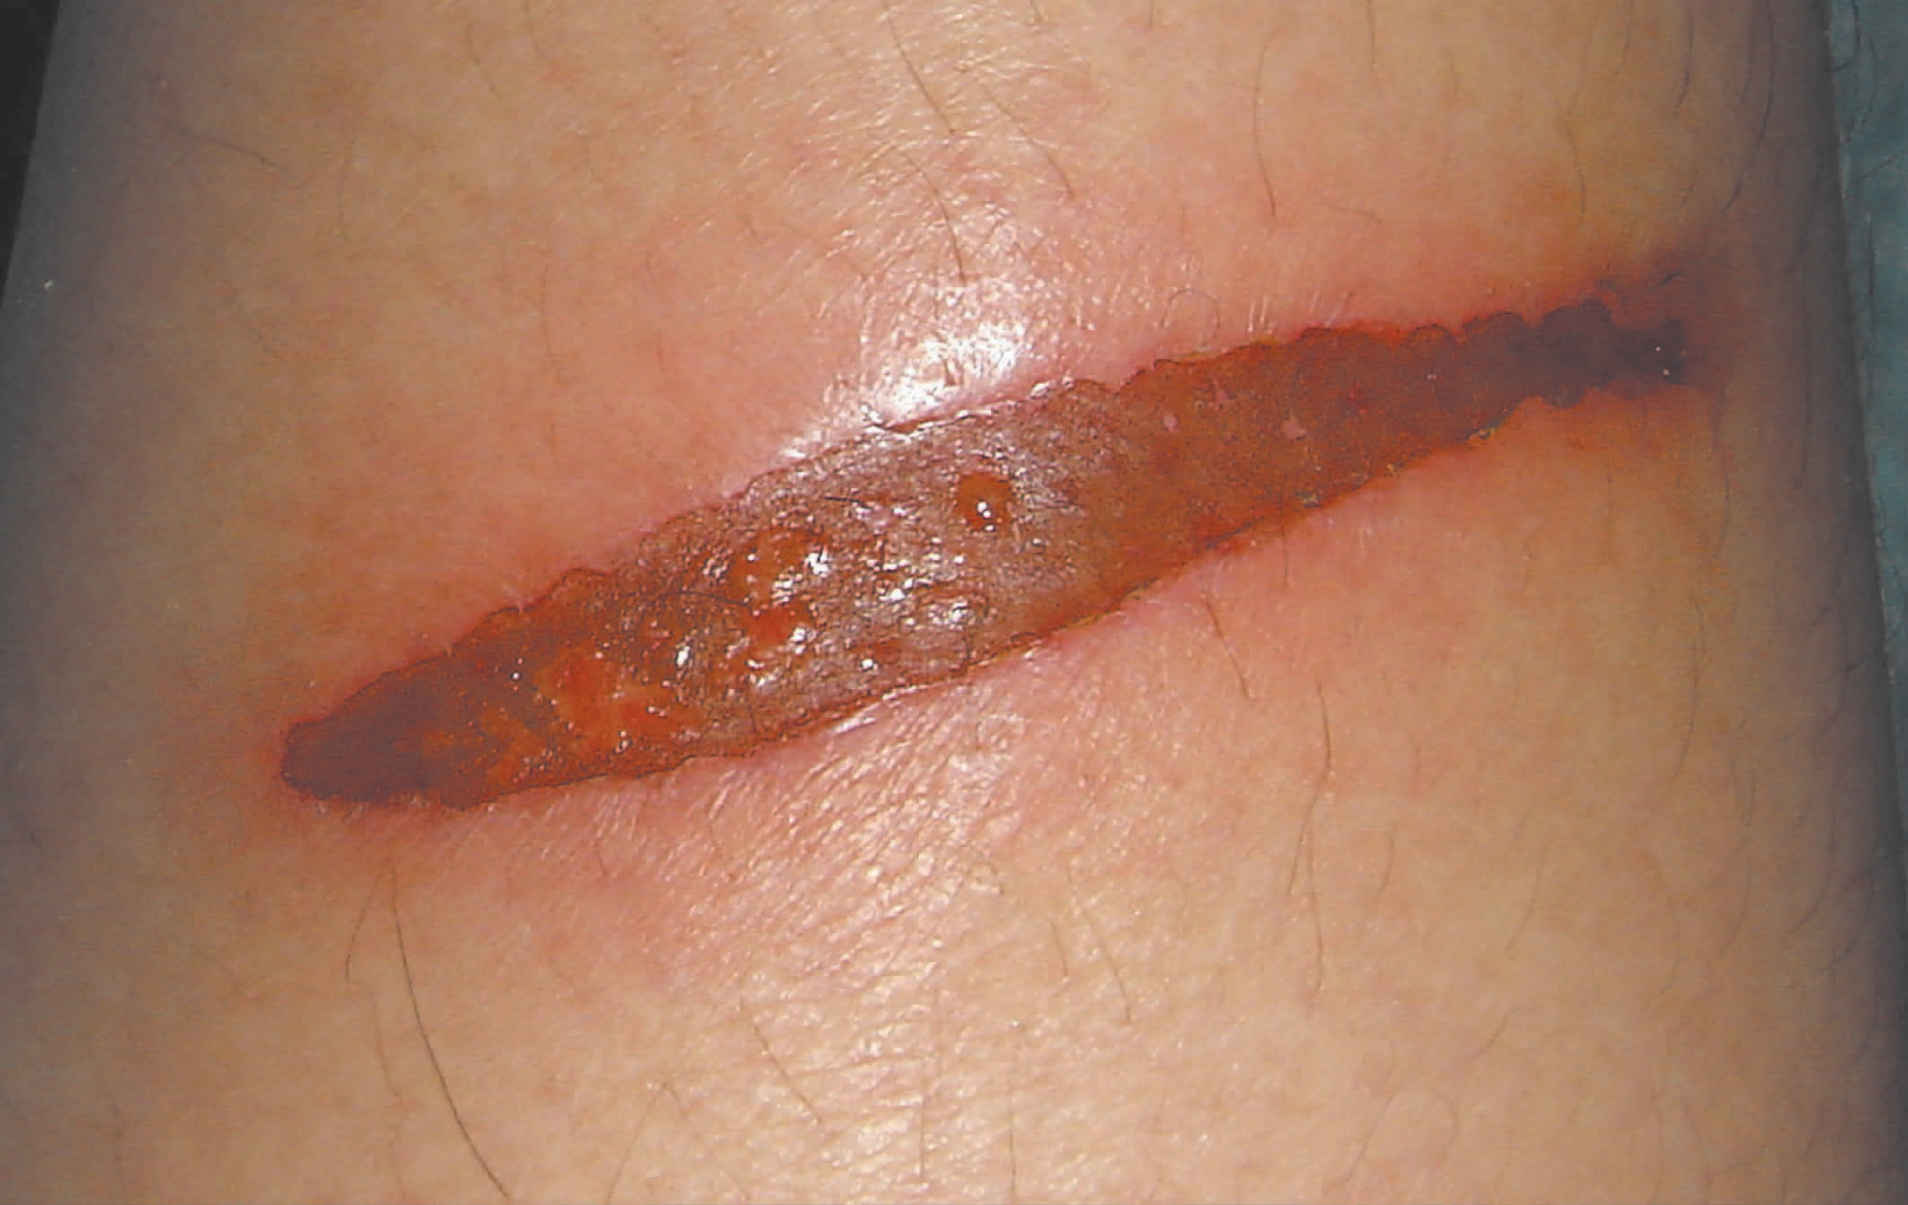
\includegraphics[width=.7\textwidth,height=\textheight,keepaspectratio]{./images/Image00026.jpg}
 \captionsetup{justification=centering}
 \caption{先天性中脑导水管狭窄\\{\small  A、B为同一患者,可见第三脑室、侧脑室积水扩张,额、顶、颞叶脑实质部分残留,枕叶、部分基底核和丘脑保存,小脑和脑干发育正常,第四脑室正常}}
 \label{fig2-10}}
  \end{figure} 



\textbf{【鉴别诊断】}
应注意与松果体区和中脑肿瘤压迫所致的导水管狭窄相鉴别,但肿瘤有占位表现且导水管有移位。炎性粘连所致的导水管狭窄与本病不易鉴别。此外,积水性无脑畸形大脑结构几乎完全消失、脑室基本无残留,枕叶一般相对完整,可予鉴别。

\subsection{结节性硬化症}

本病又称为Bourneville病,是一种较少见的常染色体显性遗传病,发病率约为1/50000~2/10000。

\textbf{【病理】}
病理特征为皮质结节、白质内异位细胞团和脑室内的小结节。结节可发生于皮质、室管膜下,皮质结节最常位于额叶,其次枕叶,偶见于基底节、丘脑、小脑和脑干。皮质结节内含有细胶原纤维、奇异的胶质细胞或不典型的神经元,多数有钙化。脑白质内异位细胞团也是由胶质细胞和神经节细胞组成。室管膜下结节最易钙化,易伴发室管膜下巨细胞型星形细胞瘤,也可伴有视网膜的错构瘤及其他内脏肿瘤。皮质腺瘤由皮质腺、结缔组织和血管组成,但国外有学者认为面部多发的不是皮脂腺瘤,无皮脂腺样结构,而是血管纤维瘤。

\textbf{【临床表现】}
典型的三联征为:①皮质腺瘤占90%;②癫痫发作;③智力低下。但三者不一定同时出现。皮质腺瘤主要位于面颊、鼻、额或两耳处,为对称散发、针头大小、黄红色透亮的坚硬蜡状丘疹。本病还可有眼、心、肾、肺、骨骼病变。

\textbf{【CT表现】}
有以下几方面:①皮质结节:可见脑回扩大、增宽,结节呈低密度,周围为等密度厚皮质围绕。一般无强化,故有人称为空心型病灶。此外,还可呈“H”型皮质结节(低密度病灶中间有一等密度横道)和高密度团块。②室管膜下结节:位于脑室边缘,50%以上双侧对称多发,结节大小不等,部分钙化,未钙化部分强化著(图\ref{fig2-11})。③室管膜下区星形细胞瘤:常位于室间孔附近。④脑白质内异位的细胞丛:皮髓交界区或更广泛的白质内见一些更低密度区。⑤其他:可有脑沟增宽等脑萎缩表现;阻塞室间孔可有脑积水表现。

\begin{figure}[!htbp]
 \centering
 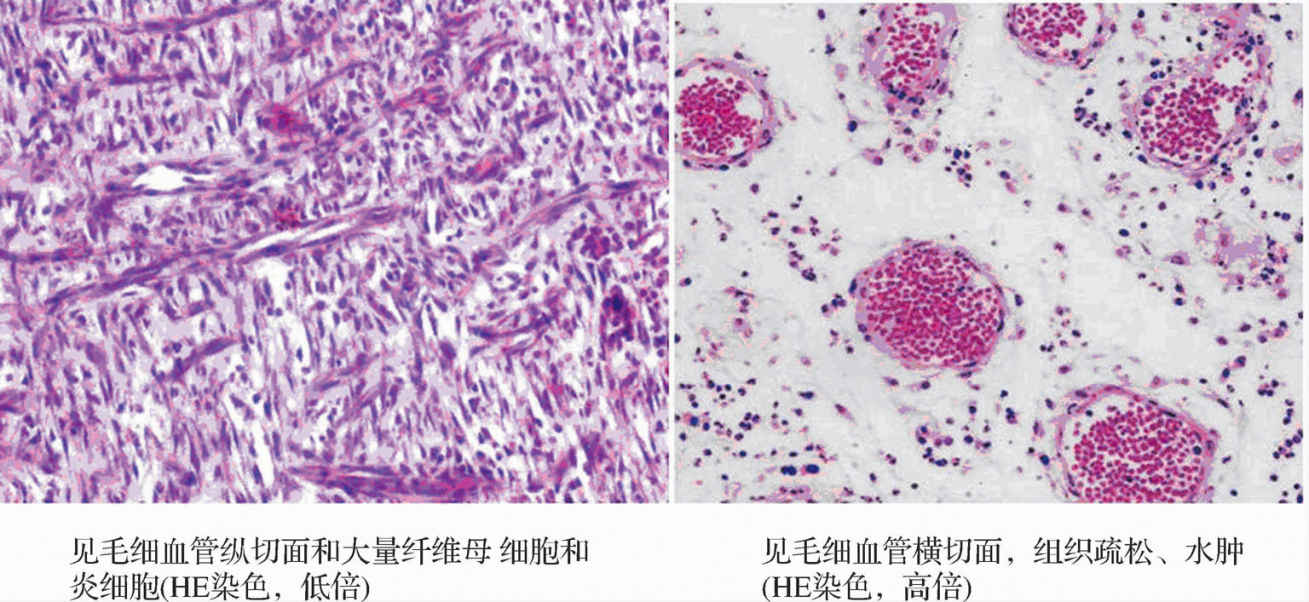
\includegraphics[width=.7\textwidth,height=\textheight,keepaspectratio]{./images/Image00027.jpg}
 \captionsetup{justification=centering}
 \caption{结节性硬化症\\ {\small 左右侧侧脑室边缘可见多个钙化结节,大小不等;右侧额叶有局限性萎缩表现}}
 \label{fig2-11}
  \end{figure} 



\subsection{脑颜面血管瘤病}

本病又称Sturge-Weber综合征或软脑膜血管瘤病。

\textbf{【病因病理】}
此病多为散发,很少有家族遗传史,偶为常染色体显性遗传。病变的分布特点为面部三叉神经分布区皮肤毛细血管瘤和同侧颅内软脑膜血管瘤,病侧大脑发育不良或萎缩。由于软脑膜血管瘤长期压迫或继发性脑缺血可引起皮质梗死,神经节细胞减少、变性,神经胶质增生伴皮质钙化,30%可发生青光眼与脉络膜血管瘤。

\textbf{【临床表现】}
癫痫、痴呆、智力低下,轻偏瘫、偏盲,先天性青光眼、牛眼症(先天性白瞳症)等,还可合并阴睾、脊柱裂等。面部分布葡萄酒色的血管痣,称作火焰痣或葡萄酒斑,出生时即可存在,主要分布在一侧三叉神经分布区,一般同颅内软脑膜血管瘤位于同一侧,但少数也可位于双侧或对侧面部。此外,约5%~15%的患者无面部血管痣。

\textbf{【CT表现】}
患侧皮层曲线状或脑回状钙化为本病特征(图\ref{fig2-12})。患侧大脑皮质萎缩伴脑沟裂、脑池增宽增深及同侧脑室扩张,钙化周围可见梗死灶,偶见出血灶。同侧脑室脉络丛有时增大,颅盖骨板障可增厚。增强扫描钙化灶周围及钙化区可明显强化;增大的脉络丛(亦属血管瘤)有明显强化。在发现脑实质内的缺血缺氧、胶质增生和脱髓鞘改变方面CT不及MR。

\begin{figure}[!htbp]
 \centering
 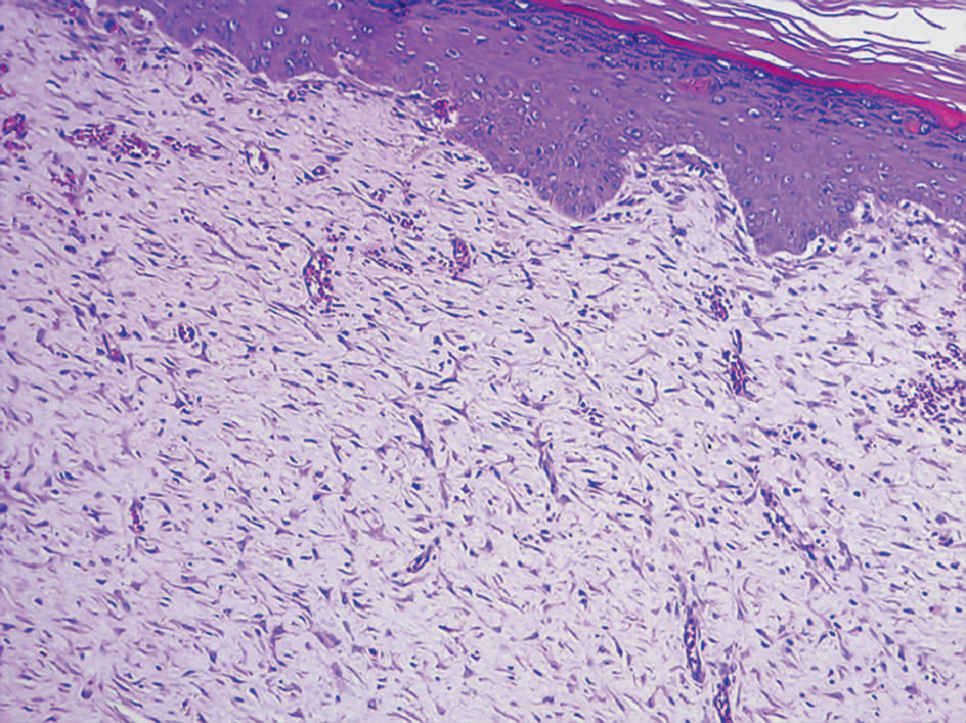
\includegraphics[width=.7\textwidth,height=\textheight,keepaspectratio]{./images/Image00028.jpg}
 \captionsetup{justification=centering}
 \caption{Sturge-Weber综合征\\{\small 右侧额叶皮层曲线状钙化,局部脑沟增宽增深}}
 \label{fig2-12}
  \end{figure} 



\textbf{【鉴别诊断】}
颅内类似的脑回状钙化也可见于胶质瘤、脑梗死、化脓性脑膜炎、骨化性脑膜脑病,故应结合本病的其他征象及临床特征予以鉴别。

\subsection{共济失调性毛细血管扩张症}

本病又称Louis-Bar综合征,是一种常染色体隐性遗传性疾病,发病率约1/40000,主要发生在儿童,男女发病相近。

\textbf{【病理】}
主要病理改变是小脑皮质萎缩,尤以蚓部为甚,齿状核-橄榄体退变、脑干中的轴索肿胀。小脑血管异常可能是其病因。

\textbf{【临床表现】}
主要特征是小脑机能障碍(共济失调),进行性眼皮(可涉及眼结膜)毛细血管扩张。患儿易患鼻窦炎、肺部感染,以及淋巴系统肿瘤。

\textbf{【CT表现】}
主要表现为以蚓部为主的小脑萎缩。小脑沟增宽增深、数目增多,小脑下蚓发育不良,四脑室扩张,小脑周围蛛网膜下腔、脑池增宽。如伴脑实质毛细血管扩张破裂,可出现脑出血。有时可见脑梗死,由来自肺内血管畸形的栓子所致。

\subsection{神经纤维瘤病}

本病是中胚层和神经外胚层的常染色体显性遗传病。

\textbf{【病理】}
主要是神经外胚层结构的过度滋生、中胚层异常发育及多发性肿瘤形成,可累及全身各系统和器官。有学者将本病分为以下5型。Ⅰ型:为局限性神经纤维瘤病,以丛状神经瘤为特征;Ⅱ型:为全身性皮肤神经纤维瘤病,以多发性皮肤结节及皮肤色素斑为主要表现;Ⅲ型:为深部周围神经干的神经瘤、神经纤维瘤和神经鞘瘤,以深部神经干过分受累为特征;Ⅳ型:为颅神经干的神经瘤、神经纤维瘤、神经鞘瘤,以双侧听神经瘤为多见;Ⅴ型:为并发脑瘤和脑瘤样变,可合并脑膜瘤、胶质瘤、血管瘤、黑色素瘤、结节性硬化、脊髓空洞症、播散性胶质结节增生等。其中Ⅰ型最常见,约1/1000神经纤维瘤可恶变。

颅内最常见的肿瘤有听神经瘤(多为双侧)、视神经胶质瘤、三叉神经瘤、基底节和丘脑部胶质瘤及多发性脑膜瘤等。此外,还可有脊神经根或马尾的神经纤维瘤、脊膜瘤,颅骨和脊柱发育异常也较常见。

\textbf{【临床表现】}
本病可见于任何年龄,但在10~20岁和50~70岁有两个发病高峰期,男多于女。其临床特点是皮肤可见特征性棕色斑(奶油咖啡色素斑)伴皮肤软组织肿块以及各组织的肿瘤形成,可有轻度思维障碍和癫痫。约1/2病例有骨骼改变(系中胚叶发育障碍和神经纤维瘤侵蚀所致),还可并发甲状旁腺功能亢进和肢端肥大症。

\textbf{【诊断标准】}
美国国立卫生研究院的诊断标准如下:①体表至少有5个直径>5mm的咖啡斑;如果是青春前期,则应有6个以上且直径>15mm;②临床或组织学证实有2个以上的神经纤维瘤或丛状神经纤维瘤;③在腋窝或腹股沟部出现多发性雀斑;④蝶骨翼结构不良或伴有骨发育畸形;⑤双侧视神经的神经胶质瘤;⑥裂隙灯检查示虹膜有2个或更多的Lish结节;⑦患者一级亲属中患有本病。具备其中两条或两条以上即可诊断为本病。

\textbf{【CT表现】}
颅内肿瘤常见的是听神经瘤,其次为三叉神经和颈静脉孔区神经纤维瘤;脑膜瘤约半数多发;偶并发胶质瘤,可发生于视交叉、脑干与基底核处。脑发育异常可有脑大畸形、胼胝体发育不全、Chiari畸形、巨脑回畸形、灰质异位等。脑血管异常有动脉瘤、动静脉畸形和动静脉瘘等。眶内肿瘤可为视神经纤维瘤、脑膜瘤或胶质瘤。脊髓肿瘤可以是马尾神经纤维瘤、脊膜瘤或室管膜瘤。

\subsection{小儿21-三体综合征}

本病又称先天愚型、Down综合征,是常见的染色体异常疾病,21号染色体三体是生殖细胞在减数分离过程中,发生不分离所致。

\textbf{【病因病理】}
与母亲妊娠时的年龄(年龄越大发病率越高)、遗传因素、妊娠时化学药物堕胎、放射线、自身免疫性疾病有关。本病主要病理变化为中枢神经系统发育异常。患儿染色体核型为47,XX(XY),+21,双亲核型正常。

\textbf{【临床表现】}
患儿表现在出生时就很显著,有的体征到1岁时才明显。根据其特殊的愚型面容、皮纹特征和智能落后容易诊断。

\textbf{【CT表现】}
①脑内钙化:多见于基底节区,呈点状或小圆形;②大脑发育不良:侧裂、额顶区蛛网膜下腔增宽;③小脑发育不良:轻度对称性小脑发育不良常见于本病;④脑干可变小,桥小脑角池、枕大池相应增大;⑤
<1岁的婴儿CT可表现正常,可能与病程演变有关。

\textbf{【鉴别诊断】}
本病应注意与结节性硬化、甲状旁腺功能减退(图\ref{fig2-13})、弓形体病、Fahr病相鉴别。

\begin{figure}[!htbp]
 {\centering
 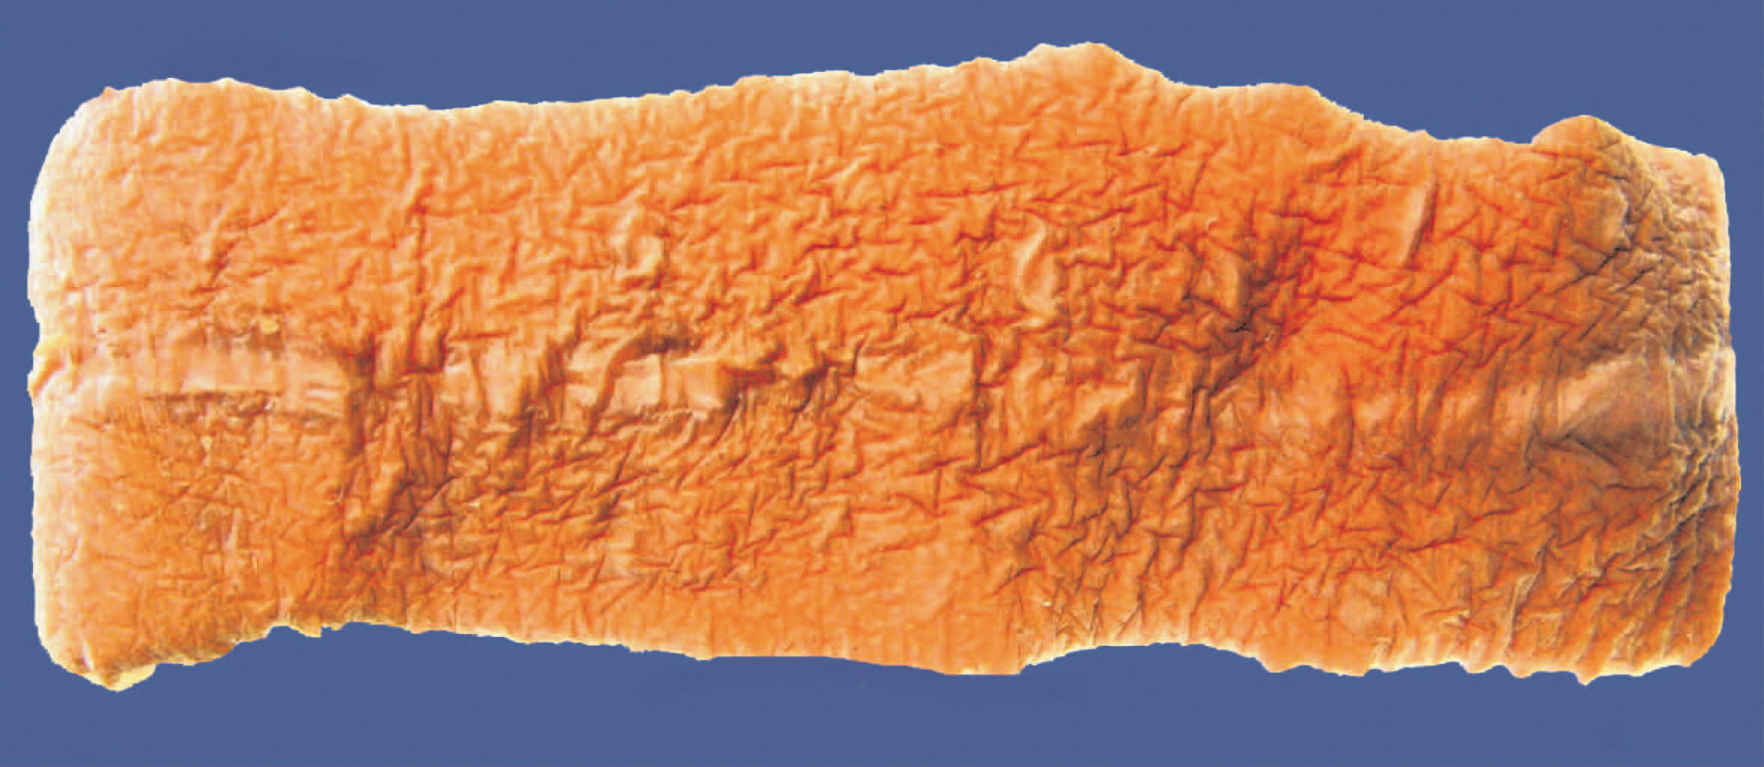
\includegraphics[width=.7\textwidth,height=\textheight,keepaspectratio]{./images/Image00029.jpg}
 \captionsetup{justification=centering}
 \caption{甲状旁腺功能减退\\{\small  A、B为同一患者,男14岁,左右侧基底核、左右侧丘脑、皮髓质交界处广泛对称性钙化}}
 \label{fig2-13}}
  \end{figure} 



\section{新生儿及婴幼儿脑疾病}

\subsection{正常新生儿和早产儿脑的CT特点}

\subsubsection{正常新生儿的脑CT表现}

1.白质密度较低:与新生儿脑组织水分含量多(且与胎龄成反比)有关。正常新生儿的脑白质密度为18~28Hu(平均>21Hu),脑灰质为26~39Hu(平均31Hu)。

2.灰白质分界模糊:人脑传导系统从胎龄7个月开始发育,神经纤维逐渐从白质伸向灰质,但出生时为数尚少,且髓鞘形成尚不完全;同时小儿脑富含蛋白质,而脂类含量少,故灰白质交界缺乏密度差异。

3.硬膜窦密度高:与窦内血流缓慢、血容量大、富含红细胞和血红蛋白等有关。

4.基底部脑池和第四脑室宽大:是因胎儿及新生儿大脑发育优于小脑和脑干所致,故桥前池和桥小脑角池亦显示较宽,纵裂池相对较窄。

5.透明隔间腔:8个月以前胎儿全部存在,新生儿82%存在,随年龄增长发生率下降。2~5周岁时为5%~6%,5~9周岁时为2.7%,10~14周岁为2.3%。

\subsubsection{早产儿的脑CT表现}

早产儿脑发育不成熟,脑组织含水量高,脑髓质化不完全,缺乏髓鞘形成,在颅脑CT扫描时可存在较广泛的或弥漫性白质低密度区,皮层灰质较薄,密度相对较高(图\ref{fig2-14}B),灰白质分界清楚,且与颅骨、脑室间形成良好的对比。

\subsection{新生儿缺氧缺血性脑病}

本病是围产期缺氧引起的脑部损害,在小儿CT检查中占7.2%,在新生儿CT检查中占94%,甚至有报道达94%~100%。

\textbf{【病因病理】}
主要病因是窒息,由宫内窒息引起的占50%,娩出过程窒息的占40%,其余10%由生后肺部疾病、呼吸暂停、红细胞增多症、败血症、先心病等所致。缺氧导致细胞内水肿、血管源性水肿,进而发生脑坏死,并由于血管通透性增加和脑血管调节失调、静脉压升高而发生颅内出血。

\textbf{【临床表现】}
可分为3度:①轻度:表现兴奋、易激惹、肢体颤动、肌张力高、反射活跃,症状于1天内好转。②中度:嗜睡、反应迟钝、肌张力低、反射减弱、惊厥、呼吸不规则,症状于1周内消失,可有后遗症。③重度:神志不清、肌张力松软、反射消失、反复发生惊厥、呼吸不规整、瞳孔不对称、对光反应消失,常在1周内死亡,存活者可有脑瘫、脑积水、智力低下、癫痫等后遗症。

\textbf{【CT表现】}
主要为脑水肿、颅内出血及脑组织坏死。①脑水肿:是早期重要征象,脑实质密度(主要是白质密度)减低,CT值≤18Hu,好发于额、顶叶。前囟隆起、颅缝增宽,脑沟、回浅扁且脑室变窄,脑室、脑池受压(图\ref{fig2-14}A)。②颅内出血:多为蛛网膜下腔出血,但脑外伤亦可致蛛网膜下腔、硬膜下、脑室内或脑室周围出血。③脑组织坏死:早产儿脑组织坏死好发于室旁白质又称为室旁白质软化,也可液化形成软化灶。

\begin{figure}[!htbp]
 {\centering
 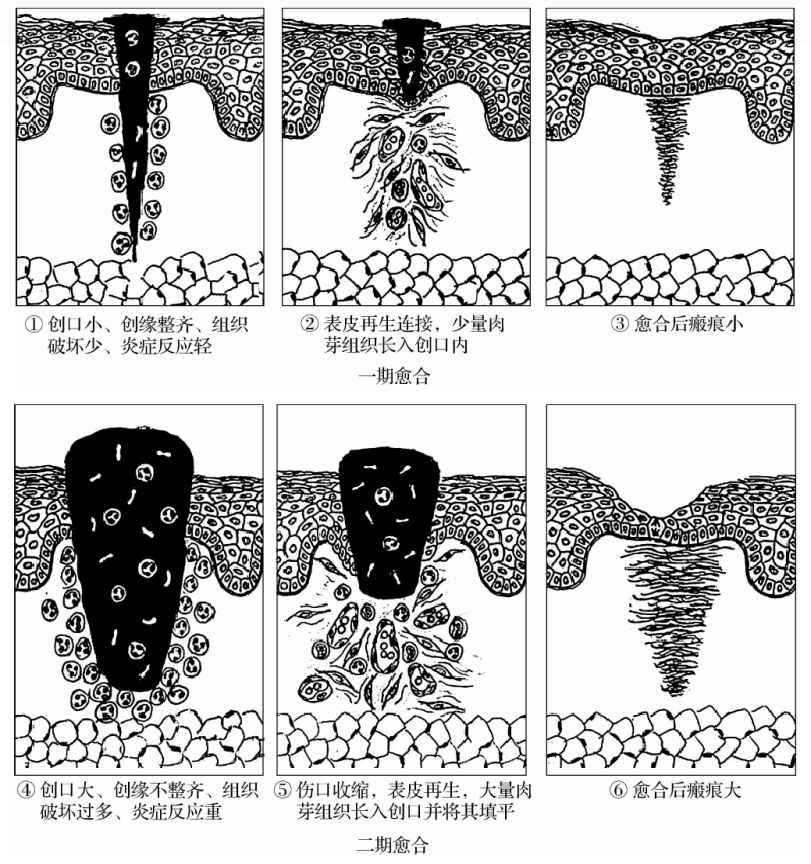
\includegraphics[width=.7\textwidth,height=\textheight,keepaspectratio]{./images/Image00030.jpg}
 \captionsetup{justification=centering}
 \caption{新生儿缺氧缺血性脑病\\{\small  A.左右额、顶叶白质区云絮状低密度灶,CT值约14~16Hu;B.皮层灰质薄,密度相对较高,灰白质分界欠清楚}}
 \label{fig2-14}}
  \end{figure} 



\textbf{【CT分度】}
①轻度:脑实质低密度影分布于1~2个脑叶,少数合并少量颅内出血(多为蛛网膜下腔出血)。②中度:低密度影超过2个脑叶,灰白质界限模糊,部分脑沟消失,约1/3合并颅内出血。③重度:弥漫性低密度影,灰白质界限消失。基底节、丘脑密度正常,脑室受压变窄,并发颅内出血者约占80%。

但我们认为对于超过2个脑叶者,如位于各叶的病灶面积均较小,且灰白质界限较清晰者,应诊断为轻度,以便于与临床分度相对应。

\textbf{【并发症】}
①轻度者于1~2个月病变多吸收,无明显后遗症。②中度者大多数亦可治愈,少数可出现外部性脑积水、脑发育不良、脑萎缩等。③重度者约35%于1周内死亡,存活者多有后遗症如脑萎缩、脑皮质变薄、脑白质减少、脑白质变性、脑软化、脑穿通畸形、钙化等。有报道病变处CT值<12Hu的重度患者多有并发症。

\textbf{【鉴别诊断】}
早产儿脑CT表现为较广泛的或弥漫性白质低密度区;皮层变薄、密度相对增高,呈花环状改变;灰白质分界清楚,脑室系统未见异常,中线结构无移位。早产儿缺氧性脑损伤灰白质界限模糊(图\ref{fig2-14}B),有颅内出血和脑室旁出血性脑梗死、脑室周围白质和脑白质发育不良及脑梗死等。两者CT表现有所区别,但早产儿合并缺氧性脑损伤时,CT难以分级。

\subsection{新生儿颅内出血}

本病是新生儿常见的急症,为新生儿死亡和以后神经发育障碍的主要原因之一。

\textbf{【病因病理】}
病因主要有新生儿缺氧缺血性脑病、产伤、早产,少数为出血性疾病、颅内先天性血管畸形。①缺氧使脑组织充血、水肿、脑血管壁通透性增高,引起渗血或点状出血;同时缺氧可使肝脏合成凝血因子发生障碍,从而加重出血。②产伤可造成硬膜窦撕裂或皮质桥静脉、脑内的静脉以及脉络丛静脉破裂。出血常见部位为硬膜下,其次为蛛网膜下腔,也可发生于脑实质、脑室内或硬膜外。③原发性出血性疾病、颅内先天性血管畸形引起的出血很少见,前者多位于蛛网膜下腔,后者可在蛛网膜下腔或脑实质内。

\textbf{【临床表现】}
少量出血时可无症状,量多时可出现激惹、尖叫、惊厥、烦躁不安、呕吐等症状,2天后出现抑制症状如嗜睡、拒奶、昏迷、四肢张力低下及呼吸不规则、青紫等。

\textbf{【CT表现】}

1.硬膜下出血:多见于足月儿,常有头皮血肿、颅骨骨折、颅缝分离。

2.蛛网膜下腔出血:最常见,有3个特征性征象。①空三角征:又称矢状窦旁征,血液积聚于矢状窦旁呈高密度,静脉窦内流动的血液呈相对低密度,底边为颅骨,形成空心形△征象。②高脚杯征:又称天幕缘征,即血液沉积于小脑幕缘上下形成“Y”或“V”形高密度影。③纵裂池边缘模糊征:即纵裂池内出血高密度影边缘模糊。以上3个征象的出现率可达50%~80%(图\ref{fig2-15})。此外,有学者认为“直窦”宽>5mm可认为有出血。

\begin{figure}[!htbp]
 {\centering
 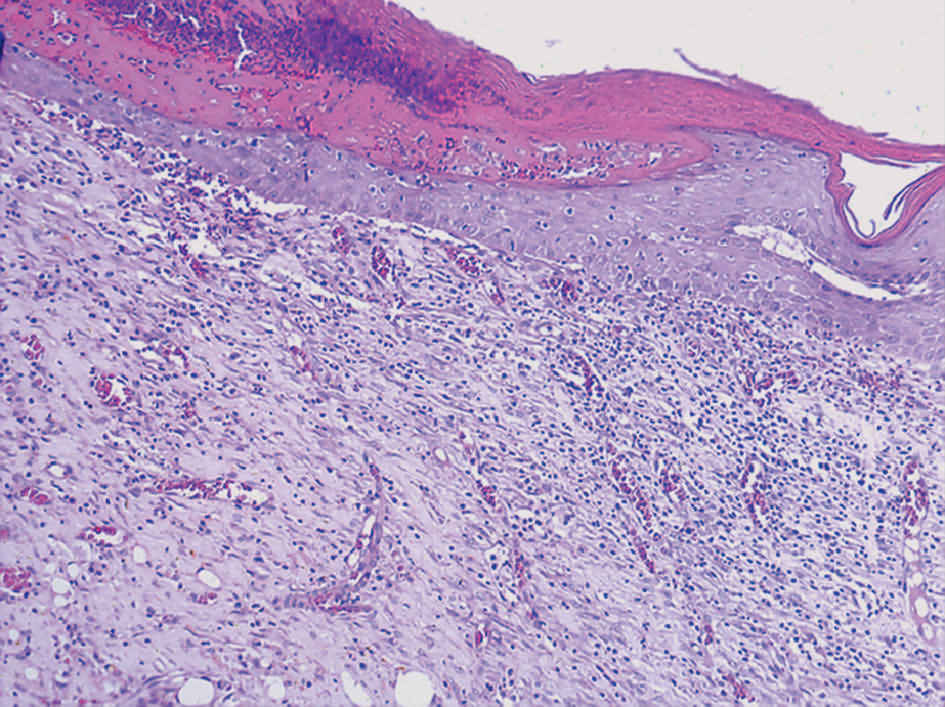
\includegraphics[width=.7\textwidth,height=\textheight,keepaspectratio]{./images/Image00031.jpg}
 \captionsetup{justification=centering}
 \caption{新生儿蛛网膜下腔出血\\{\small  A.高脚杯征;B.空三角征,伴有脑室内出血;C.纵裂池边缘模糊征}}
 \label{fig2-15}}
  \end{figure} 



3.脑实质内出血:呈点状或斑片状高密度灶,有或无水肿带。

4.室管膜下及脑室内出血:常见于早产儿。因室管膜下胚胎生发层组织发育不成熟,血液极易渗出,多量渗出可破入侧脑室,并可致脑积水。

5.其他:包括硬膜外出血和小脑出血,均较少见。

\textbf{【鉴别诊断】}
①钙化:新生儿颅内出血CT值为50~80Hu,新生儿颅内钙化少见且均为病理性,CT值>80Hu,因此不难鉴别。②晚发性维生素K缺乏症:发病年龄多在1~2个月小婴儿,出血量大、部位多,常有血团块形成、液平面出现及伴有脑梗死、大面积水肿,可予鉴别。

\subsection{婴儿维生素K缺乏症}

本病又称迟发性维生素K缺乏症、晚发性维生素K缺乏症,是指新生儿晚期(出生后2周)至乳儿期,因缺乏维生素K而引起的出血性疾病。

\textbf{【病因病理】}
常见的原因有3种:①维生素K摄入不足;②合成障碍;③吸收不良。维生素K是合成多种凝血因子所必需的辅酶,缺乏凝血因子凝血活性丧失,造成自发出血。

\textbf{【临床表现】}
发热、惊厥抽搐、呕吐、烦躁不安、拒乳、嗜睡等;可伴皮肤、消化道、上呼吸道出血等,并出现相应表现。婴儿期特别是1~4个月内母乳喂养儿若出现进行性贫血、全身出血倾向并伴急性颅内高压等精神症状应首先考虑本病。实验室凝血时间、凝血酶原时间延长及部分凝血活酶原时间延长可肯定诊断。

\textbf{【CT表现】}
①颅内出血:特点为出血量大,多发部位出血(脑实质内、外或脑室等);②脑水肿、脑梗死:是由于血管受挤压或痉挛所致,可呈广泛小片状水肿表现或大面积梗死,甚至半球缺血性改变;③脑疝;④一侧侧脑室闭塞,对侧侧脑室扩张积水;⑤并发症:存活者可致外部性脑积水、脑软化、脑萎缩、脑穿通畸形或脑发育不良。

\subsection{新生儿胆红素脑病}

持久性或明显的新生儿高胆红素血症可以导致脑部损伤。

\textbf{【病因病理】}
最常见的原因是红细胞溶血,其他原因包括红细胞增多症、胆红素结合方面的遗传或获得性缺陷、消化道运转方面的疾患及激素的紊乱等。未结合胆红素进入脑组织,结合于脑细胞膜,抑制细胞线粒体酶的活性,使脑细胞能量代谢障碍,致脑部损伤。

\textbf{【临床表现】}
足月儿常在生后2~5天,早产儿常在7天左右发生本病。典型的临床表现分为4期:①警告期;②痉挛期;③恢复期;④后遗症期。

\textbf{【CT表现】}
尚无报道本病有特异性CT表现。MR在急性期呈短T1和长T2信号;慢性期苍白球、下丘脑和海马显示长T2信号。

\subsection{血钠过高性脱水}

\textbf{【病因病理】}
最常见的原因是严重的腹泻,钠在细胞间隙中浓度升高致细胞内液体减少并皱缩。脑离开颅板导致桥静脉撕裂,另外血液的高渗致毛细血管增粗,易发生毛细血管破裂及脑实质出血。

\textbf{【临床表现】}
年幼儿童,尤其是未成熟儿对血钠过高有易感性。病儿极度冷漠、对刺激易激性高,另外还有肌肉强直、反射亢进,偶有癫痫。

\textbf{【CT表现】}
间质水肿引起脑实质密度降低,在大脑和小脑灰白质交界处可见高密度出血灶。

\subsection{新生儿低血糖症}

低血糖的标准是足月儿血糖低于16.7mmol/L(300mg/L),未成熟儿低于11mmol/L(200mg/L)。大多数低血糖的新生儿发病早,持续时间短,对葡萄糖反应迅速。但足月小样儿在子宫内就遭受营养不良,大多有临床症状,低血糖程度相对较重,持续时间可以延长,治疗需大量的葡萄糖。引起脑损害最通常的原因是继发于胰腺β细胞的先天性肿瘤或增生性胰岛素分泌过多。

\textbf{【CT表现】}
围产期低血糖脑损害表现为:①急性期:皮质和皮质下白质的脑水肿,以顶枕部最重;②慢性期:皮质和皮质下白质萎缩。

\subsection{外部性脑积水}

本病亦称良性蛛网膜下腔增宽,是一种特殊的交通性脑积水。一般2岁内自愈。

\textbf{【病因病理】}
有新生儿缺氧缺血性脑病、出血、外伤、感染等,半数病因不明为特发性。其发病机制可能为蛛网膜颗粒对脑脊液的吸收障碍所致。多数学者认为颅缝开放是其发生的前提。

\textbf{【临床表现】}
抽搐(约占50%以上)和头围增大(占1/3~2/3);部分患儿无症状。抽搐的发生与本病的严重程度密切相关。本病好发于2~24月前囟未闭的小儿,但可在生后数天发生,3~6个月为典型期,9个月~1岁开始好转,2岁前或囟门闭合前基本恢复正常。

\textbf{【CT表现】}
额叶或额、顶叶蛛网膜下腔间隙>5mm,而后部不宽。前纵裂池增宽>7mm,后纵裂池不宽。外侧裂池增宽>7mm。鞍上池稍大。额、顶叶脑沟部分增宽,但增深不著。大脑后半部及小脑正常。脑室正常或轻度扩大(图\ref{fig2-16})。

\begin{figure}[!htbp]
 {\centering
 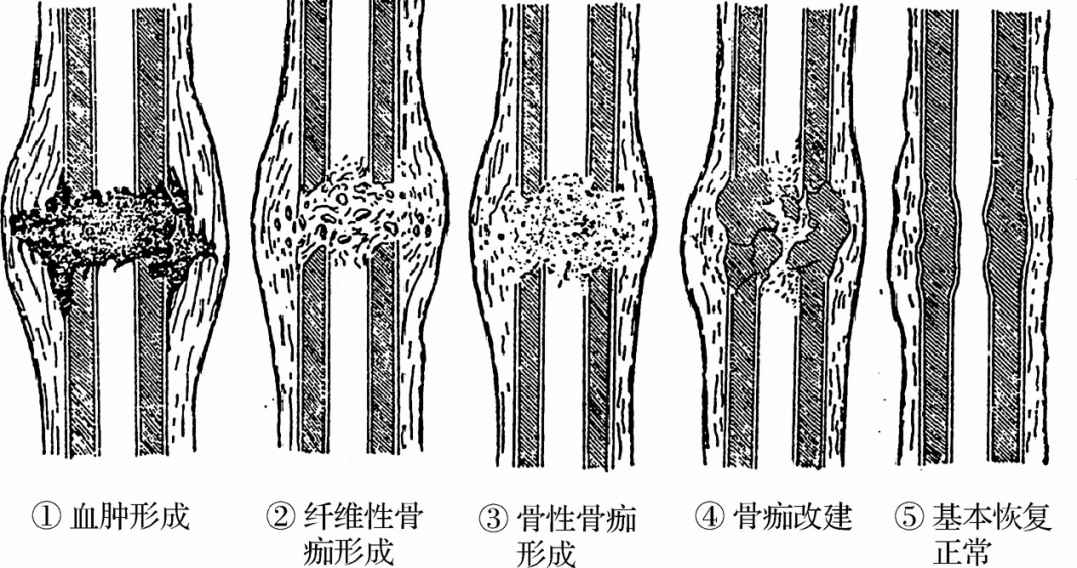
\includegraphics[width=.7\textwidth,height=\textheight,keepaspectratio]{./images/Image00032.jpg}
 \captionsetup{justification=centering}
 \caption{外部性脑积水\\{\small  A、B为同一患者,额、顶叶蛛网膜下腔间隙>5mm,而后部不宽;前纵裂池增宽>7mm,后纵裂池不宽;外侧裂池增宽>7mm}}
 \label{fig2-16}}
  \end{figure} 



总之,本病诊断的依据是:①前囟未闭的婴儿及头颅增大;②脑前部脑外积液增多,脑实质无改变;③2岁后脑外积液自然吸收。

\textbf{【鉴别诊断】}

1.在诊断外部性脑积水时,应除外其他因素引起的蛛网膜下腔增宽,其中包括促肾上腺皮质激素和皮质类固醇的治疗、脱水、营养不良以及癌肿化疗等。

2.脑萎缩:①外部性脑积水头围大,常有抽搐,无智力低下及运动障碍;而脑萎缩头围小,常有智力低下及运动障碍。②前者仅脑的前部蛛网膜下腔增宽;而脑萎缩常全脑蛛网膜下腔及脑沟增深、增宽。③前者纵裂池增宽限于前部;而后者则为整个增宽。④前者脑皮质厚度正常,脑沟可增宽但增深不著;而后者脑皮质变薄,密度减低及脑沟普遍加深。⑤脑室大小不能用于两者的鉴别,因为外部性脑积水可有轻度脑室增大。但脑萎缩时脑室与颅脑横径之比大于正常,而外部性脑积水正常。双额叶局限性脑萎缩时鉴别有一定难度,其双侧额角的局限扩大有助于与外部性脑积水鉴别。

3.硬膜下积液:本病多为单侧,双侧时常不对称,脑沟相互聚拢而不是加深加宽,不难鉴别。

4.脑发育迟缓:多表现为灰白质比例失常,常合并其他多种神经系统畸形。

\subsection{儿童脑室周围白质软化症}

本病又称为脑室周围萎缩、脑室周围白质发育不良,多认为好发于早产儿及产后窒息存活的儿童。

\textbf{【病因病理】}
与缺血缺氧及感染有关,主要损伤轴索及少突胶质细胞,但发病机制尚不清楚。病变主要分布于侧脑室三角区及枕角周围白质、额角附近白质。病理上脑白质由于缺血缺氧发生水肿、凝固、坏死,继而吸收或形成瘢痕和胶质增生,弥漫或局限的胶质损伤使髓鞘化延迟、白质减少,从而导致侧脑室扩张。

\textbf{【临床表现】}
本病可以导致脑瘫(主要是痉挛性下肢瘫或四肢瘫)、智力落后、抽搐,以及各种眼的异常如眼颤、斜视、视力下降等。

\textbf{【CT表现】}
显示脑室周围和半卵圆中心的脑白质明显减少,皮质与脑室缘距离甚小或消失,也可见呈斑片状或长条状的软化灶(图\ref{fig2-17})。一侧或两侧侧脑室扩大,扩大的脑室轮廓不规则可与脑积水鉴别。

\begin{figure}[!htbp]
 \centering
 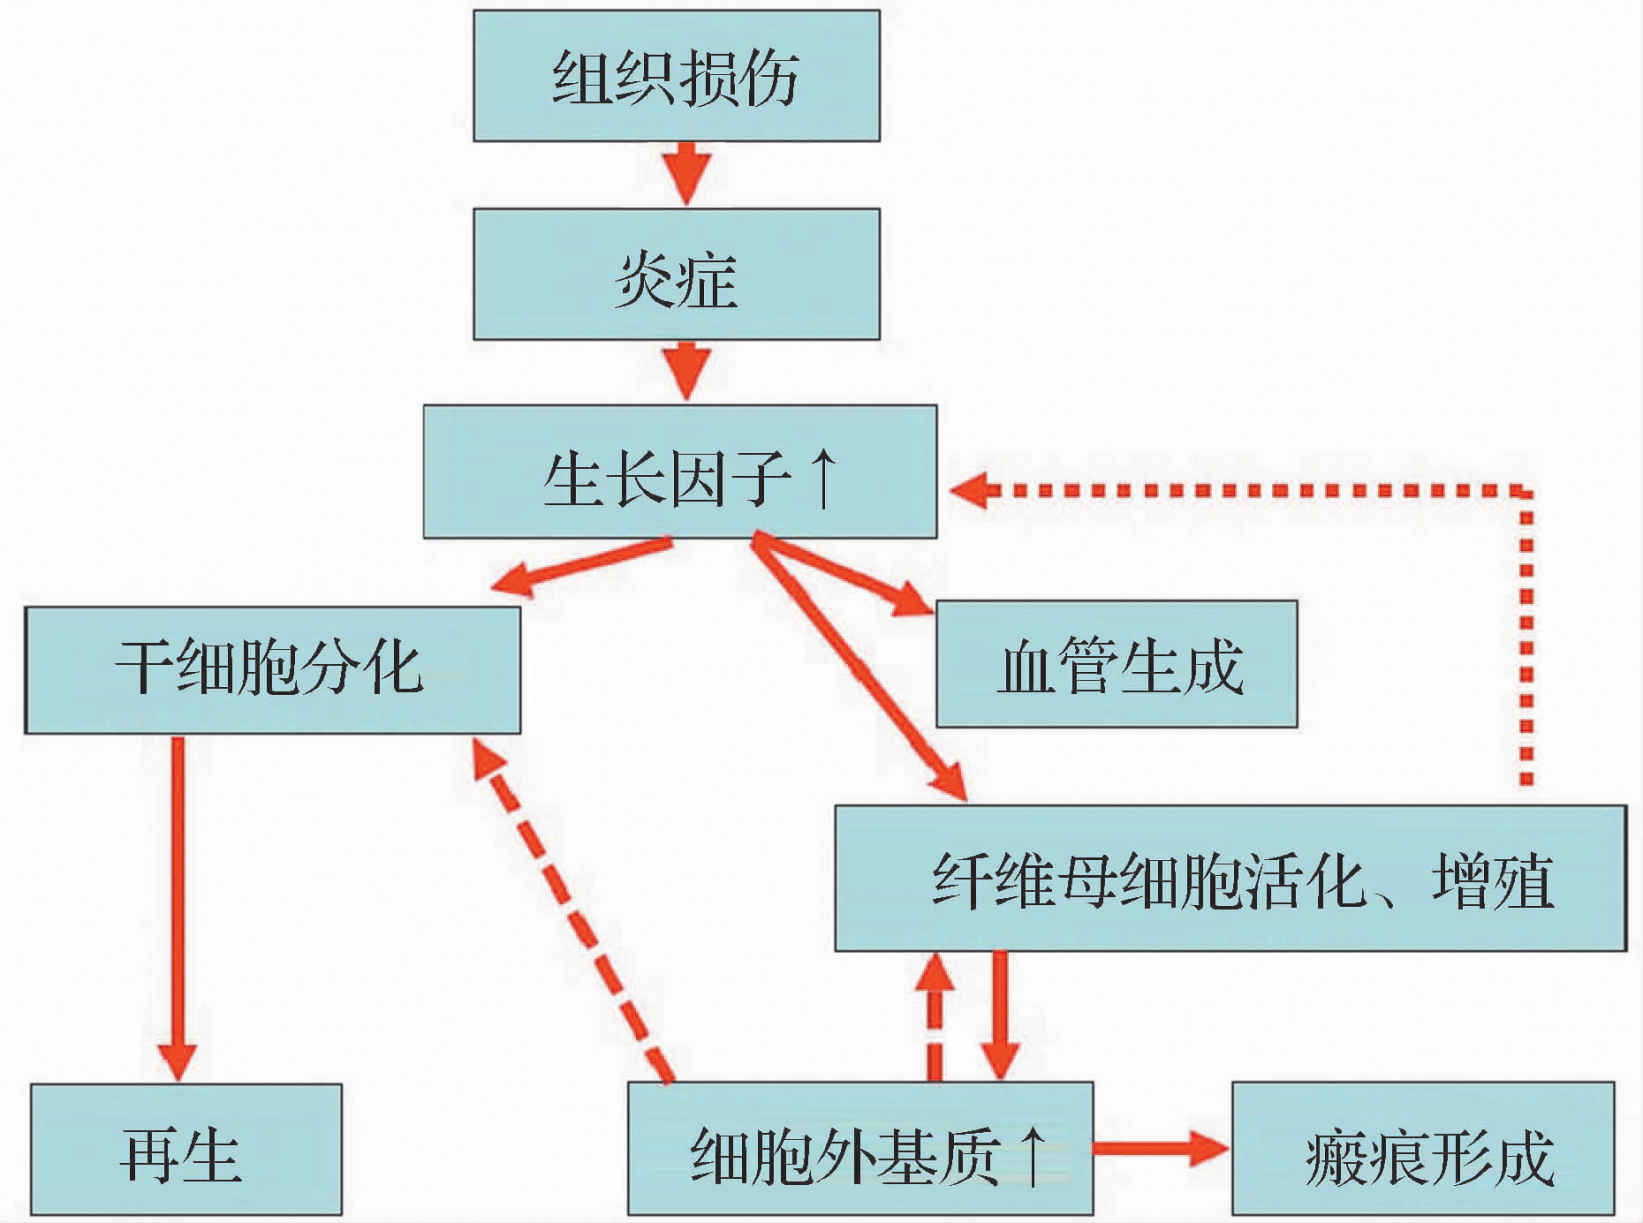
\includegraphics[width=.7\textwidth,height=\textheight,keepaspectratio]{./images/Image00033.jpg}
 \captionsetup{justification=centering}
 \caption{脑室周围白质软化症\\{\small 脑室周围和半卵圆中心的脑白质明显减少(右侧显著),皮质与脑室缘距离甚小,右侧有斑片状软化灶}}
 \label{fig2-17}
  \end{figure} 



\subsection{儿童脑性瘫痪的相关疾病}

本病是指出生前至出生后1个月内各种原因所致的非进行性脑损害综合征。临床表现为中枢性运动障碍及姿势异常,可伴智力低下、癫痫、视力障碍及行为异常。其CT改变可分为以下6种类型。

1.脑发育畸形:可分为器官源性和组织源性(已于上节详述)。

2.脑萎缩:大多由于缺血性损害或颅内感染导致脑白质或灰质减少、丧失,是脑性瘫痪最常见的CT表现。①可表现为脑沟裂增宽、增深,脑室增宽等。②其中脑室周围白质软化(PVL)约占脑萎缩的65%。③小脑萎缩可见小脑上沟增多(3条或3条以上)。

3.脑软化灶:多发生于较成熟的脑组织,可能与新生儿缺氧缺血性损害及颅内出血有关。

4.基底节病变:多由于脑血管阻塞致脑缺血缺氧性损害以及颅内感染、出血或中毒引起苍白球、丘脑区铁钙质沉着及神经细胞变性坏死。CT表现一侧或两侧对称性钙化灶或软化灶。

5.混合型:即上述两种以上病变混合存在。

6.正常:其原因可能为:①CT未能显示全部病灶或遗漏;②少数脑瘫与病变部位神经递质异常有关,CT不能显示;③胎儿期囊性病灶出生后自行消失;④CT检查的局限性,如CT难以显示矢状窦旁区脑损害及髓鞘形成延迟或发育不良。

\section{脑积水}

\subsection{概述}

1.脑积水:是指由于脑积液的产生和吸收不平衡所致的脑室扩大。按其发病机理可分为两大类:①脑脊液循环或吸收障碍;②脑脊液分泌增加。后者非常少见,主要见于脑室肿瘤如脉络丛乳头状瘤。脑脊液的吸收过去认为是通过蛛网膜颗粒,20世纪70年代后认为它不是惟一的吸收途径,并有学者认为主要是通过中枢神经系统表面吸收。

2.交通性脑积水:是指第四脑室出口以下的正常脑脊液通路受阻或吸收障碍所致的脑积水。国外有学者提出交通性脑积水应改称为动脉搏动限制性脑积水。动脉搏动明显减弱可能是由于动脉壁变硬或蛛网膜下腔顺应性降低所致。但动脉压并没有降低且传递的更远,使脑内脉压增高,大脑皮层压力梯度增大,脑室系统扩大。

3.阻塞性脑积水:又叫做非交通性脑积水,是指脑室系统即第四脑室出口以上任何部位发生阻塞所造成的脑积水,是最常见的脑积水。

脑积水时侧脑室旁白质内,CT上可见不规则低密度,是由于间质性水肿所致。即在脑室内压力增高时,室管膜受损出现小裂隙,水分子由此进入侧脑室周围白质内形成间质性水肿。高血压、动脉硬化及部分脑萎缩病人也可在室旁白质内出现上述CT表现(或异常MR信号),但其机理与脑积水不同,可能与局部组织变性、胶质增生、细胞萎缩后间隙扩大等有关。

\subsection{交通性脑积水}

\textbf{【病因】}
主要有蛛网膜下腔出血、脑膜炎、颅脑损伤以及静脉栓塞,亦可见于脑膜瘤病、脑脊液吸收功能障碍等。

\textbf{【临床表现】} 主要表现为颅内压增高的症状和体征。

\textbf{【CT表现】}
典型表现是脑室系统普遍扩大;另一特征是脑沟变浅、变平(但也可正常甚至扩张)。早期为颞角扩大和钝圆,稍后为额角扩大,进一步加重出现第三脑室扩大,第四脑室扩大较晚,与脑萎缩相比第三脑室扩大更明显。但有时交通性脑积水表现不典型,特别合并脑萎缩时,诊断较困难。此外,蛛网膜下腔出血和化脓性脑膜炎可表现为急性脑积水,脑室系统短时间内明显扩大。

交通性脑积水的特征之一为脑沟变浅、变平且灰白质界限清楚,常据此帮助诊断。但有时脑沟、脑池扩大,特别是纵裂池、基底池和桥小脑角池扩大。这种情况多见于基底池等有关脑池的炎症或肿瘤所致的部分脑脊液循环通路受阻及脑脊液吸收障碍。

脑室旁白质水肿发生率约为40%,且长期存在的交通性脑积水往往不出现这种征象。这是因为长期室内高压所致的室管膜受损,发生胶质增生形成室管膜瘢痕,阻止了脑脊液渗漏。

\subsection{正常压力性脑积水}

本病是交通性脑积水的一种特殊类型,多发生在慢性交通性脑积水的基础上,部分完好的脑脊液循环吸收功能代偿,且脑脊液的分泌功能下降,从而形成新的平衡。此时,虽然脑室系统仍明显扩大,但脑脊液压力正常,故又称为常压性脑积水。但实际上,大多并不一直正常,呈波动性。

\textbf{【临床表现】}
一般无颅内高压征,可能由于扩张侧脑室对周围白质的压迫,出现痴呆、步态不稳等症状。

\textbf{【CT表现】}
多不典型。由于脑室内压力正常,可在脑室扩大的同时出现脑沟加深,但两者不呈比例,脑室扩大更著。

\subsection{阻塞性脑积水}

\textbf{【病因病理】}
主要有先天性疾病、感染性疾病和肿瘤。病理表现为脑实质变薄,并可继发脑萎缩、白质脱髓鞘、胶质增生和神经细胞退行性变。

\textbf{【临床表现】}
主要为颅内压增高的症状和体征。其中先天异常、胎儿期或出生过程中发生该病者多在婴幼儿期出现症状,有的至10岁后或成年才表现异常。患儿有头颅增大,两眼球下旋形成“落日征”等甚有特点。

\textbf{【CT表现】}
阻塞近侧脑室扩大,阻塞远侧脑室形态正常或缩小(图\ref{fig2-18})。侧脑室旁间质水肿较明显而且范围广泛,脑沟也可变浅平,有时可见脑室疝。但病因诊断较困难。

\begin{figure}[!htbp]
 {\centering
 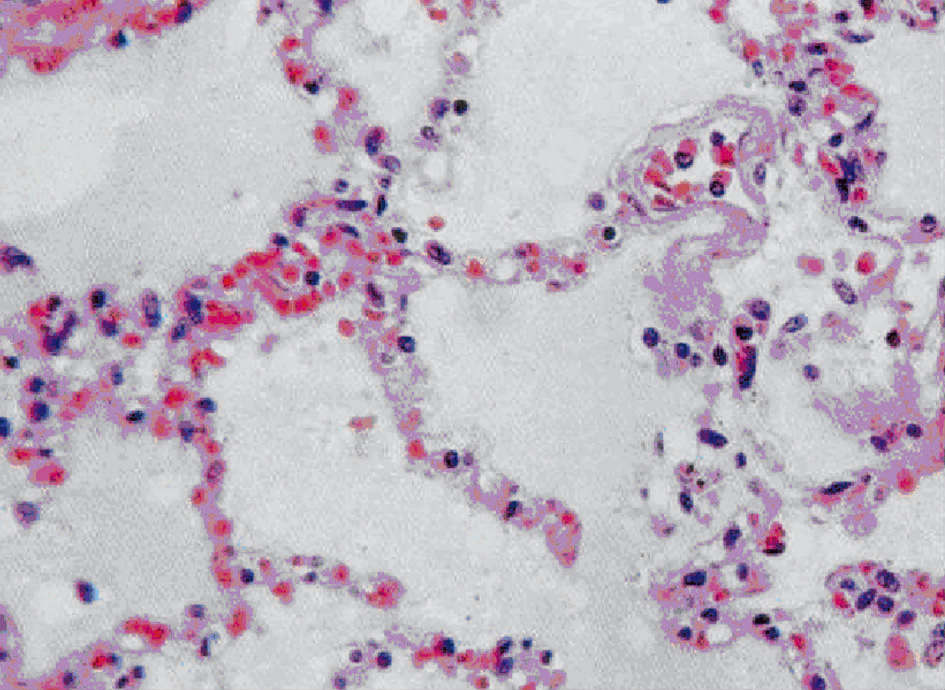
\includegraphics[width=.7\textwidth,height=\textheight,keepaspectratio]{./images/Image00034.jpg}
 \captionsetup{justification=centering}
 \caption{阻塞性脑积水\\{\small  A、B为同一患者,第三脑室、侧脑室扩大(第四脑室正常)}}
 \label{fig2-18}}
  \end{figure} 



先天性患者可重度积水,表现幕上大脑半球区为水样低密度,额、顶、颞叶脑实质几乎消失或残留极少,部分枕叶、基底核和丘脑保存(图\ref{fig2-10})。

\textbf{【鉴别诊断】}
与交通性脑积水鉴别时,如果阻塞在中脑导水管或以上,由于第四脑室不扩大,则两者容易鉴别。如阻塞部位在第四脑室出口时则两者难以鉴别。脑池造影观察第四脑室与蛛网膜下腔的通畅情况有助于鉴别。

\subsection{脑积水与脑萎缩的鉴别诊断}

主要有以下几点:①脑积水的扩大是均匀性和中心性扩张,尤其侧脑室前角呈气球状;而脑萎缩的脑室形态改变不及脑积水明显,特别是室旁脑组织较少的部位变形轻微,如第三脑室前壁、漏斗隐窝和视隐窝。②脑积水时由于颅内压力较高,脑沟变浅或消失,脑池亦不增大;而脑萎缩涉及皮质时脑沟加深、脑池扩大。③阻塞性脑积水和脑萎缩均可致一侧脑室扩大或一侧脑室扩大明显。在阻塞性脑积水时脑室可向扩大或扩大明显的对侧移位;而脑萎缩则向同侧移位。④脑积水侧脑室旁白质内可见间质性水肿所致的低密度;但脑萎缩因室旁白质变性亦可出现低密度灶。⑤脑萎缩是以白质为主的萎缩,表现为侧脑室边缘不规则,有助于与脑积水鉴别。

\section{脑萎缩}

\subsection{概述}

\subsubsection{脑变性疾病和脱髓鞘疾病的概念}

这是两组病变累及部位不同的神经系统疾病。前者累及神经元(灰质);后者累及髓鞘(白质),为髓鞘脱失,而轴索相对完好(见本章第十一节)。但两者均可引起脑萎缩。

变性疾病的特点是某一或二个功能系统的神经细胞发生萎缩和死亡,星形细胞增生。受累部位不同,临床表现也不同。如累及大脑皮质主要表现为痴呆;累及基底节、锥体外系则引起功能障碍;累及小脑引起共济失调。

脑变性疾病按部位分为:①大脑皮质:如Alzheimer病、Pick病。②基底节及脑干:如Jakob-Creutzfeldt综合征、Huntington舞蹈病、Parkinson病、进行性核上麻痹、Sky-Drager综合征。③脊髓及小脑:如橄榄桥脑小脑萎缩、原发性小脑萎缩、共济失调性毛细血管扩张症。④运动神经元:如脑萎缩性侧索硬化、脊髓性肌萎缩。

\subsubsection{脑萎缩的概念}

1.脑萎缩:是指由于各种原因所引起的脑组织减少而继发的脑室和蛛网膜下腔扩大。这种脑组织减少可分别或同时累及脑白质和脑灰质,其病因很多。根据其累及范围可分为局限性和弥漫性两类,但有时两者很难完全分开。

2.局限性脑萎缩:脑实质以局限性容积缩小为主,表现为局限性脑沟增宽和脑室、脑池扩大,有时仅发生于一侧半球。此外,还可见局部脑组织密度下降。

3.弥漫性脑萎缩:脑实质的减少为弥漫性,表现为脑室和蛛网膜下腔扩大广泛(图\ref{fig2-19})。可根据累及灰、白质程度的不同将其分为皮质型和中央型。前者以累及灰质为主,脑沟增宽明显,而脑室扩大次之;后者主要累及白质,以脑室扩大为主,脑沟扩大为次。

\begin{figure}[!htbp]
 \centering
 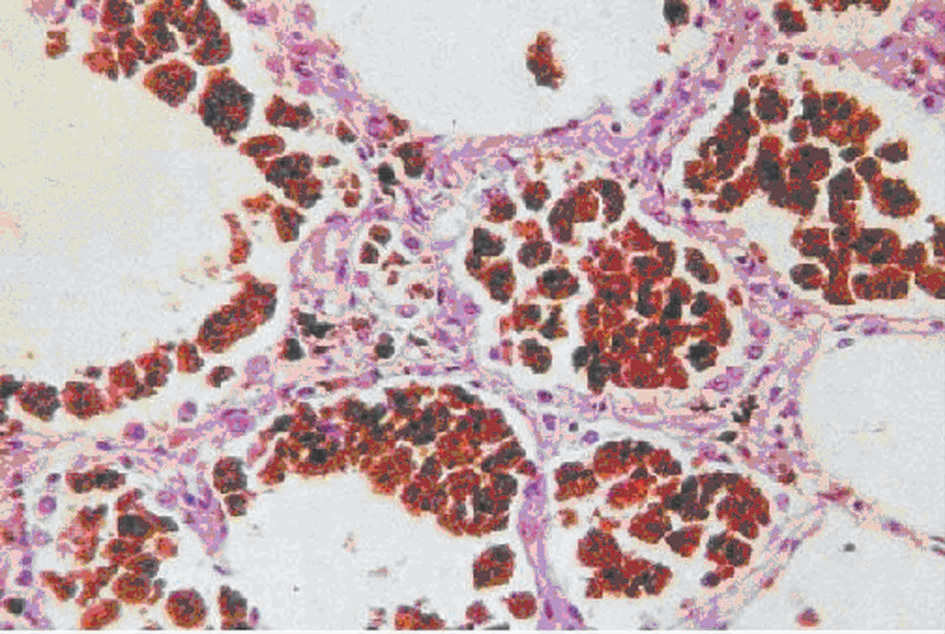
\includegraphics[width=.7\textwidth,height=\textheight,keepaspectratio]{./images/Image00035.jpg}
 \captionsetup{justification=centering}
 \caption{弥漫性脑萎缩\\{\small 脑室和蛛网膜下腔广泛扩大,室旁白质内有低密度灶,侧脑室边缘不规则}}
 \label{fig2-19}
  \end{figure} 



\subsubsection{局限性脑萎缩的病因}

1.外伤性脑萎缩:一般发生在外伤3~6个月后,少数外伤可造成弥漫性脑萎缩。

2.感染后脑萎缩:多继发于脑脓肿,颅内低毒性感染有时可造成弥漫性脑萎缩。

3.脑梗死后脑萎缩:一般发生在发病后3~6个月。

4.Pick病:又称脑叶萎缩症,系常染色体显性遗传性疾病。多见于女性,病程5~6年,呈进行性恶化。临床表现智力低下、痴呆、共济失调等,与Alzheimer病难以区别。但本病以额叶和颞叶萎缩为主,尤其以两额叶为著;而Alzheimer病为弥漫性脑萎缩,且以颞叶较著,额叶多不明显。

5.大脑半球萎缩:由于胎儿期或新生儿期血管阻塞引起的大块脑梗死所致,一般在青少年期才被发现。

\subsubsection{弥漫性脑萎缩的病因}

临床上较局限性脑萎缩更常见,多见于正常老年人,亦可见于许多病理情况。①Alzheimer病;②Huntington病;③Parkinson病;④Wilson病;⑤脑缺氧;⑥Jakob-Creutzfeldt综合征;⑦肿瘤和代谢失调:均与脑组织营养障碍有关(肿瘤患者虽无脑转移瘤,但可有营养障碍),同样情况也可见于AIDS、肝性脑病、血液透析者、慢性酒精中毒和肥胖病人;⑧药物性脑萎缩:如类固醇、氨基甲叶酸、度冷丁、酒精等使用不当。

\subsection{老年脑(生理性脑萎缩)}

关于老年脑的临床意义,目前认识尚不统一。这是因为正常情况下随着年龄的增加,脑组织和其他器官一样,逐渐老化而发生萎缩即所谓生理性萎缩。但随着年龄的增加,易发生的高血压、脑动脉硬化等因素均可损害脑组织而发生萎缩,这种萎缩虽与年龄有关,却为病理性。相对而言生理性萎缩较病理性萎缩轻,但两者无明显界限。

\textbf{【CT表现】}
老年脑主要表现为脑室、脑池轻度扩大和脑沟轻度增宽,多为两侧对称。脑沟增宽以额叶、镰旁顶叶显著,脑室扩大以侧脑室额角、颞角和第三脑室显著。

\subsection{Alzheimer病(爱茨海默病)}

本病以往曾称为早老性痴呆或老年前期痴呆,是一种以弥漫性脑萎缩(但以颞叶为主)为特征的痴呆。本病与老年性痴呆只有年龄上的差异而无本质的区别,故国际上将两病合并称为Alzheimer型痴呆。

\textbf{【病理】}
主要病理表现为脑萎缩,尤其是颞叶海马萎缩为主。镜下脑组织神经细胞减少,尤其有大量老年斑和神经纤维缠结时有定性价值,神经元空泡颗粒变性和淀粉样血管病变,但均为非特异性的,可见于老龄脑。

\textbf{【临床表现】}
其特征为进行性记忆力减退,语言和行为障碍。生前主要依据神经心理测验确立诊断。其病程不可逆转,一般持续3~10年,最后继发感染和全身衰竭而导致死亡。

\textbf{【CT表现】}
①弥漫性脑萎缩表现,与老年性脑萎缩相似,无特征性。②内侧颞叶萎缩是本病最早、最敏感的指征,以海马萎缩最突出,其次为额顶叶。主要表现为颞角扩大,颞叶皮质萎缩和海马回密度减低。有人取负于听眦线20\textsuperscript{o}
平面为扫描基线,层厚5mm,在环池水平测量颞角内侧边与环池外侧边的最小距离即中颞叶最小宽度,其参考值为8.67mm,小于此值即为中颞叶萎缩。③胼胝体萎缩为本病的另一指征,以嘴部和压部最为明显。④在海马萎缩的同时,MR、ECT(PET)等所显示的特异性区域血流量下降也可作为本病的特异性表现。

\textbf{【鉴别诊断】}
主要应于血管性痴呆鉴别。后者在我国老年人中占痴呆疾病的首位(西方占第二位),其颞角扩张不及Alzheimer病明显。严重的皮层下和脑室周围白质病变是多发性梗死型痴呆较典型的表现。

\subsection{慢性进行性舞蹈病}

本病又称遗传性舞蹈病、亨廷顿(Huntington)病,是基底节和大脑皮质变性的一种常染色体显性遗传性疾病。

\textbf{【病理】}
以尾状核及壳核萎缩明显,后期则额、顶叶皮质萎缩。镜下见神经元减少和胶质细胞增生。其生化改变为基底节中多巴胺含量过多,而γ-氨基丁酸及胆碱的含量减少。

\textbf{【临床表现】}
好发于20~50岁,其特征为慢性进行性舞蹈样动作和痴呆,多有遗传和家族史。

\textbf{【CT表现】}
主要为尾状核及壳核的萎缩。两侧尾状核头、体部相对缩小,可伴或不伴侧脑室(尤其额角)扩大和脑沟增宽,两侧壳核对称性低密度。一般只要出现尾状核萎缩即可以做出诊断,小脑和脑干也可萎缩。

\subsection{Parkinson病(帕金森病)}

本病又称震颤麻痹,可分为原发性和继发性两类。前者病因不明;后者可因脑动脉硬化、挫伤、基底节肿瘤、药物和化学物质中毒所致,又被称为Parkinson综合征。

\textbf{【病理】}
肉眼变化的特点是黑质和兰斑脱色。镜下可见该处的神经黑色素细胞丧失。黑质和苍白球神经元明显减少,局部萎缩及黑色素退变。中脑黑质致密带色素细胞大量丢失,桥脑兰斑色素细胞明显减少,脑有对称或非对称萎缩。黑质与兰斑均属儿茶酚胺能核团,分泌多巴胺;尾状核、壳核的神经元属胆碱能细胞,分泌乙酰胆碱。由于黑质神经元大量丧失,使多巴胺含量下降,从而使得对纹状体区乙酰胆碱的抑制作用下降,出现震颤麻痹。

\textbf{【临床表现】}
发生于中年以上,起病很缓慢,逐渐加剧。主要症状包括震颤、肌张力高(强直)、运动障碍、假面具样面容等。

\textbf{【CT表现】}
无特异性,主要为脑室扩大和弥漫性脑萎缩,有时合并基底节钙化,后者亦可见于正常人。CT所示的脑萎缩与临床所见的震颤麻痹的严重程度无明显关系。MR可有黑质(致密带)的萎缩及异常铁质沉积所致的低信号。

\subsection{肝豆状核变性}

本病又称Wilson(威尔逊)病,是一种常染色体隐性遗传的铜代谢障碍性疾病。

\textbf{【病理】}
由于肝脏合成血浆铜蓝蛋白的能力下降,引起肝脏、大脑基底节区和角膜的铜沉积,亦可累及额叶皮质、红核、黑质及齿状核及肾等处。脑受累部位变性、萎缩、胶质增生,甚至缺血坏死、软化。以豆状核软化、角膜色素环(K-F环)及小叶性肝硬化为三大主征。

\textbf{【临床表现】}
好发于10~25岁青少年,约1/3有家族史。基底节损害症状包括进行性加剧的震颤、僵直与多动症,皮质损害为衰退型精神障碍,有肝硬化和角膜色素环表现。

\textbf{【CT表现】}
少数可无异常发现。主要表现为豆状核低密度区,多为双侧,使豆状核界限不清。低密度区还可累及尾状核、齿状核、红核、额叶和丘脑等,部分还可见尾状核、大脑和小脑萎缩。

\textbf{【鉴别诊断】}

1.代谢性疾病:其中以肝豆状核变性最常见,还有亚急性坏死性脑脊髓病(Leigh病)、维生素B\textsubscript{1}
缺乏症,以及线粒体脑病、Kearns-Sayre综合征、海绵状脑白质营养不良、黏多糖病、Hallervorden-Spatz病、岩藻糖苷沉积症、先天性丙酮酸代谢障碍。

2.感染性疾病:EB病毒性脑炎、乙脑和腮腺炎病毒性脑炎等。

3.中毒性疾病:以一氧化碳中毒最常见,还有变质甘蔗中毒、大量硫化氢吸入中毒、甲醇中毒和氰化物中毒等。

此外,纹状体黑质变性(40~50岁发病,病程渐进,以帕金森综合征为首见症状,为锥体外系疾病或列入多系统变性)也可出现双侧壳核对称性低密度及全脑萎缩。国内有学者报道1例静脉窦血栓形成致双侧基底节对称性低密度。我们遇见1例尿毒症患者,表现为以内囊后肢为中心,部分涉及双侧豆状核的低密度。

\subsection{皮质纹状体脊髓变性}

本病又称Jakob-Creutzfeldt综合征、亚急性海绵状脑病、传染性病毒性痴呆。过去一直被纳入变性范围,现多认为是一种病毒感染性疾病。

\textbf{【病理】}
出现以灰质为主的明显脑萎缩。镜下皮质、大脑基底节、脊髓、小脑、丘脑、脑干及脊髓前角神经元变性。神经细胞脱失,脑实质空泡化伴胶质细胞增生,病灶区如海绵状,无炎性变化,白质多正常,晚期可受累。

\textbf{【临床表现】}
好发于40~70岁,主要表现为迅速发展的精神衰退和痴呆,并可出现锥体束、锥体外系及共济失调症状。80%死于发病后1年左右。

\textbf{【CT表现】}
大脑皮质弥漫性萎缩,脑沟、裂增宽增深,亦可见两侧脑室扩大。晚期脑白质受累可见低密度,无占位效应,无强化。本病进展快,短时间随访明显加重。

\subsection{小脑萎缩}

\textbf{【病因】}
本病可由变性性疾病、中毒、慢性酒精中毒、滥用药物等引起。发生于儿童的共济失调性毛细血管扩张症亦表现为以蚓部为主的小脑萎缩。此外橄榄桥脑小脑萎缩(或称橄榄桥脑小脑变性)也是共济失调的一个类型。

\textbf{【病理】}
病变主要在小脑、小脑脊髓束、锥体束、橄榄核,甚至累及大脑皮质,小脑萎缩皮质重于髓质。橄榄桥脑小脑萎缩除小脑萎缩外,还有桥脑、橄榄的明显萎缩,大脑皮质也可受累。

\textbf{【临床表现】}
成年发病,病程缓慢,可为10~40年。表现为小脑性共济失调,锥体束征、锥体外系征、视神经萎缩。

\textbf{【CT表现】}
应包括以下两个或两个以上征象(图\ref{fig2-20}):①小脑沟增宽>1mm(也有人认为\textgreater{}2mm);②小脑沟在半球超过2条,蚓部超过4条;③桥小脑角池扩大>1.5mm(应测量小脑上边缘与岩骨边缘间的距离);④第四脑室扩大;⑤小脑上池扩大。

\subsection{精神分裂症}

本病多有脑结构的异常。

\begin{figure}[!htbp]
 \centering
 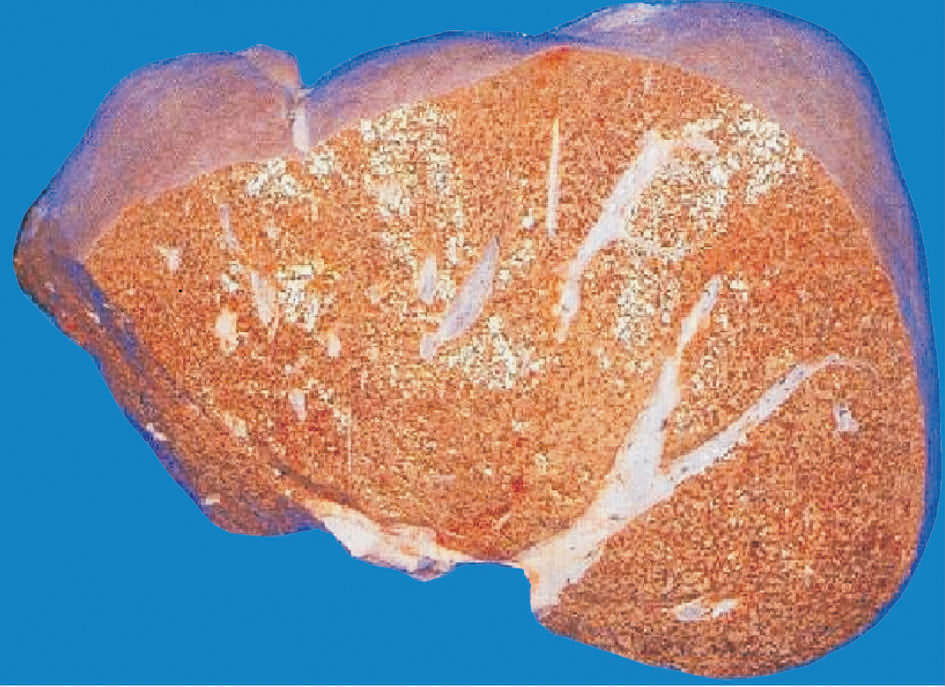
\includegraphics[width=.7\textwidth,height=\textheight,keepaspectratio]{./images/Image00036.jpg}
 \captionsetup{justification=centering}
 \caption{小脑萎缩\\{\small 小脑沟显著增宽、增多,以蚓部为著}}
 \label{fig2-20}
  \end{figure} 



\textbf{【CT表现】}
第三、第四脑室扩大,两侧裂池增宽、脑沟扩大,有时出现侧脑室扩大和小脑萎缩。两侧室旁核和小脑的密度可增加,其意义尚不肯定。

\subsection{颞叶癫痫}

颞叶癫痫的常见原因为海马硬化(又称安蒙氏角硬化和颞叶中内侧硬化)。

\textbf{【病理】} 特征为神经元丢失和胶质细胞增生,导致海马的萎缩。

\textbf{【CT表现】}
其CT诊断价值较小,仅约23.8%有异常。表现为:①颞叶内侧低密度灶;②颞角扩大;③侧裂池增宽。

\textbf{【MR表现】} 海马的萎缩(为神经元丢失的反应)、T\textsubscript{2}
WI海马高信号(为胶质细胞增生的反应)、颞叶前部萎缩以及颞角扩大。

\section{脑缺血、出血和脑血管病变}

\subsection{动脉缺血性脑梗死}

脑组织因血管阻塞引起缺血性坏死或软化称为脑梗死。广义的脑梗死除动脉缺血性脑梗死外,还包括静脉血流受阻所致的脑梗死即静脉性脑梗死。但大多习惯于狭义的将动脉缺血性脑梗死称为脑梗死。

\textbf{【病因】}
引起梗死的原因很多,可分为两大类。①脑血管阻塞:又分为血栓形成和栓塞。前者最常见的是在动脉粥样硬化的基础上形成血栓;后者是指外来栓子堵塞血管所致。②脑部血液循环障碍:是指在脑血管原有病变的基础上(亦可无原发血管病变),由各种原因造成的脑组织供血不全而引起的梗死,故又称非梗阻性脑梗死。

\textbf{【病理】}
过去将脑梗死分为3个时期,即梗死期、吞噬期、机化期。目前通常将脑梗死分为:①超急性期:6小时以内;②急性期:6小时后~2天;③亚急性期:2天后~2周内;④慢性早期:2周~1个月;⑤慢性晚期:1月后(见表\ref{tab2-2})。

\begin{table}[htbp]
\centering
\caption{脑梗死的病理过程及CT表现}
\label{tab2-2}
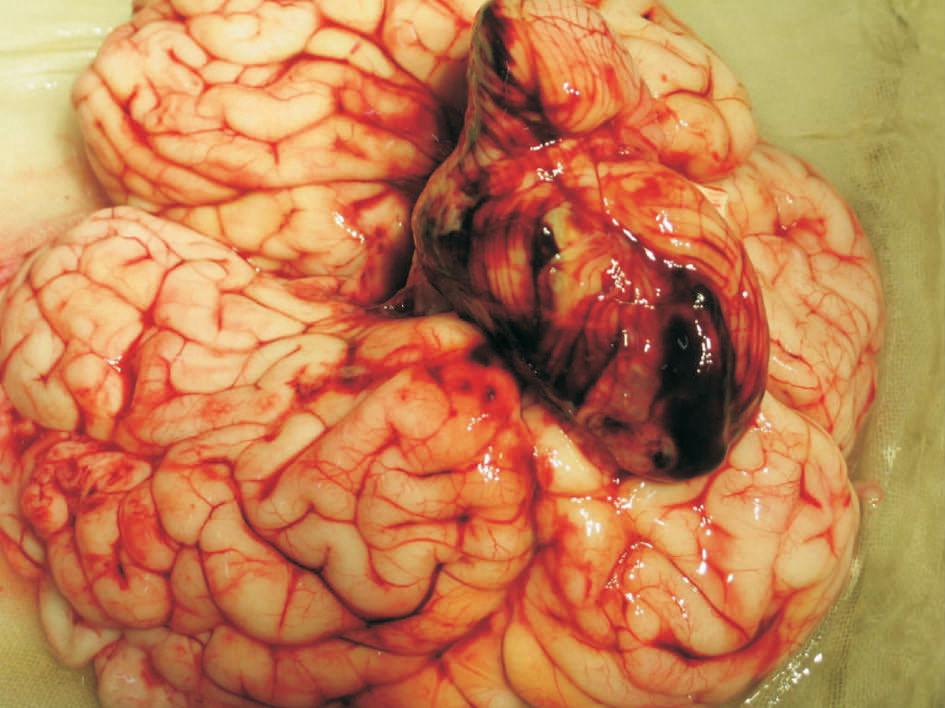
\includegraphics[width=\textwidth,height=\textheight,keepaspectratio]{./images/Image00037.jpg}
\end{table}

脑供血完全终止后数秒钟神经元电生理活动停止,持续5~10分钟以上就有不可恢复的细胞损伤。但是临床上供血血管闭塞可能不完全和(或)存在侧支循环,仅使局部血流降低到一定程度。故部分脑组织虽有缺血损伤,但仍可恢复正常,这部分脑组织区域称为缺血半暗带。它位于缺血坏死核心与正常脑组织之间。但如超急性期治疗不及时或治疗无效可发展成为完全脑梗死。

少数缺血性脑梗死在发病24~48小时后可因再灌注而发生梗死区内出血,称为出血性脑梗死。

\textbf{【临床表现】}
临床表现复杂,取决于梗死灶大小、部位及脑组织的病理生理反应。主要表现为头昏、头痛,部分有呕吐及精神症状,可有不同程度的昏迷。绝大多数出现不同程度的脑部损害症状,如偏瘫、偏身感觉障碍、偏盲,亦可失语、抽搐,较重者可有脑疝症状。从解剖学可知,皮质脊髓束有10%的纤维不交叉下降,加入同侧皮质脊髓侧束。皮质脊髓前束也有少量纤维不交叉,止于同侧颈、胸髓。这些不交叉的运动传导纤维支配了同侧肢体运动,当这些纤维受损时,导致同侧肢体出现不同程度的运动功能障碍如麻木、无力,甚至偏瘫。

\textbf{【CT表现】}

1.超急性期脑梗死的CT表现:①大脑中动脉高密度征:为高密度血栓或栓子所致,出现率约占35%~45%(敏感度78%,特异度93%),但需除外血管硬化因素。最近研究表明,此征可见于近60%的正常人(尤其用7mm以下层厚扫描),故此征的诊断价值值得怀疑。②脑实质低密度征:可能为细胞内水肿所致,可见于脑的凸面、基底节区、岛叶,有时可伴侧裂池受压。③局部脑组织肿胀征:可能为血管源性水肿所致,局部脑沟变窄以至消失,脑回增厚、变平(图\ref{fig2-21}A)。脑CT灌注成像有利于超急性期脑梗死的诊断。

此外,脑血管CTA可显示闭塞部位、程度和侧支循环情况。

许多学者研究证实,CT灌注成像可以预测半暗带,即脑血流量(rCBF)中度减低时,局部脑血容量(rCBV)无明显变化或仅有轻度下降或轻度升高,此时缺血区微血管管腔受压、变形、闭塞的程度较轻。当rCBF和rCBV均明显减低时,提示脑局部微血管管腔闭塞程度明显、微循环发生障碍、脑组织发生梗死。国内有学者将面积\textsubscript{CBV}
定义为预测的梗死面积,则面积\textsubscript{CBF} -
面积\textsubscript{CBV} 为预测的半暗带面积。

2.典型CT表现:①脑组织低密度灶,呈楔形或三角形,病灶部位、范围与闭塞动脉供血区相吻合。大脑中动脉主干闭塞,病灶呈三角形低密度区,尖端指向第三脑室;大脑中动脉闭塞在豆纹动脉的远端,病灶多为矩形低密度区,出现“基底核回避现象”。大脑前动脉闭塞表现为位于大脑镰旁的长条状低密度区。大脑后动脉闭塞在顶叶后部及枕叶可见半圆形的低密度区,位于大脑镰旁的后部。局灶性脑皮质梗死,表现为脑回丢失。室管膜下脑梗死,脑室边缘呈波浪状。一般在发病24小时后出现以上表现(图\ref{fig2-21}B、C)。②2~3周时由于“模糊效应”,病灶可偏小或消失。③脑梗死后2~15天为水肿高峰期,可有占位效应,占位效应一般见于病变范围大的病例。如占位效应超过1个月,应注意有无肿瘤可能。④增强扫描病灶周围和病灶内出现脑回状、线状、团块状强化。⑤1个月后病灶开始软化呈水样密度,病变范围大的病例可继发局限性脑萎缩。

此外,出血性脑梗死在梗死区内可见高密度出血灶(图\ref{fig2-21}D)。



\begin{figure}[!htbp]
 \centering
 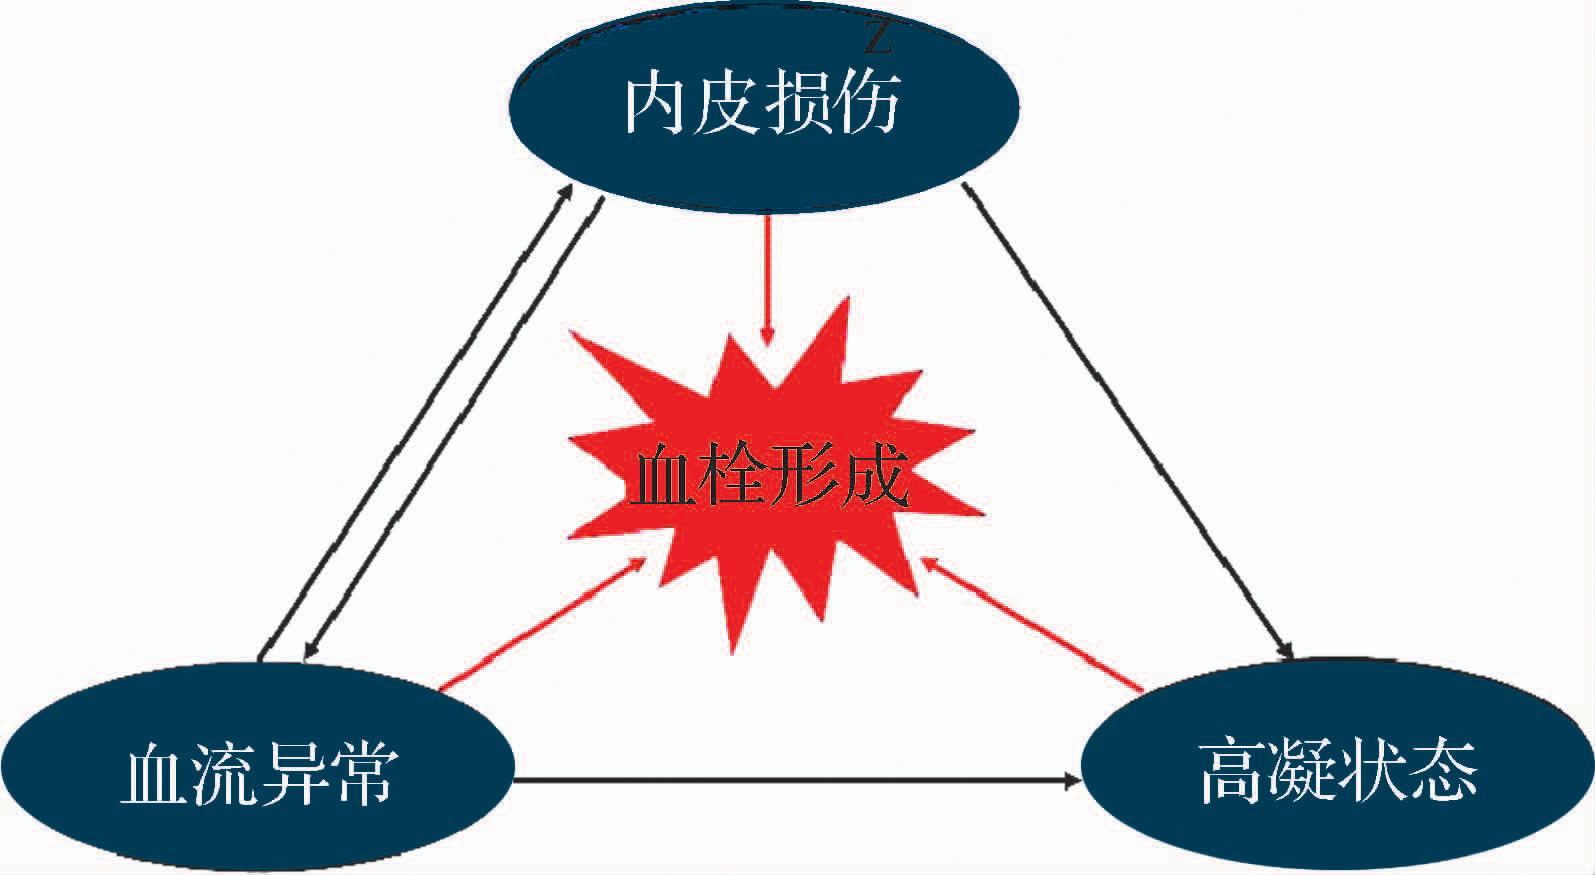
\includegraphics[width=\textwidth,height=\textheight,keepaspectratio]{./images/Image00038.jpg}
 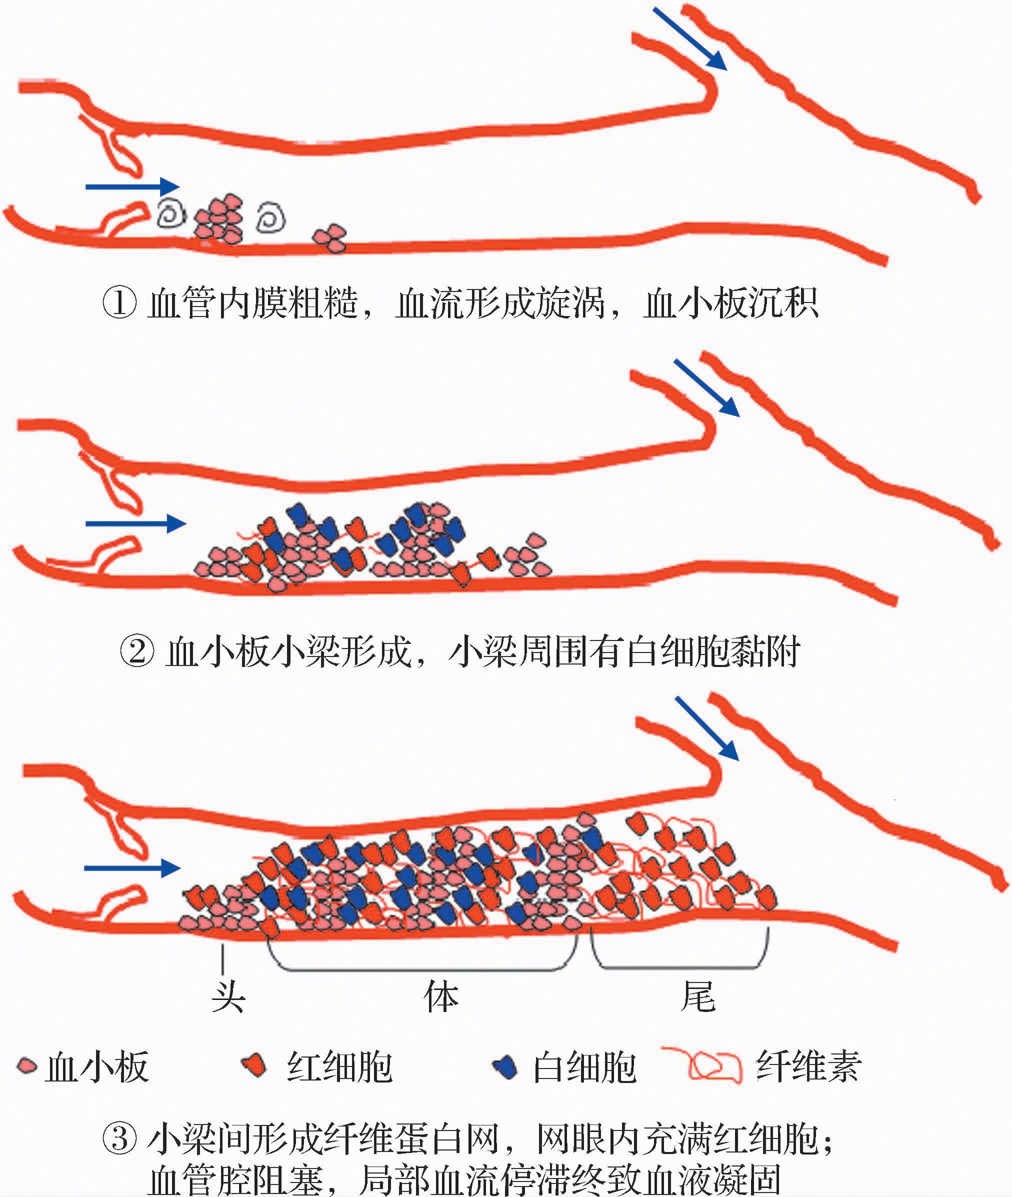
\includegraphics[width=\textwidth,height=\textheight,keepaspectratio]{./images/Image00039.jpg}
 \captionsetup{justification=centering}
 \caption{脑梗死\\{\small A、B为同一患者。A.超急性期,发病后4小时,右侧额顶叶脑沟消失,皮髓质交界不清晰;B.发病后42小时,右侧颞额顶叶大片状低密度灶,界限清晰,显著占位效应;C.亚急性期脑梗死,左侧顶额叶区有大片楔形低密度区,占位效应较显著;D.出血性脑梗死,右侧颞额叶区有大片楔形低密度区,占位效应显著,其内见大片状高密度出血灶,左侧基底节区可见水样密度的软化灶}}
 \label{fig2-21}
  \end{figure} 

3.增强扫描CT表现:梗死灶强化的形态多种多样,可表现为脑回状、线状、片状、环状,可出现在病灶的边缘和中心。而延迟30分钟~3小时扫描可显示皮质下白质强化,可能与梗塞区皮质内大量毛细血管破坏,造影剂漏出有关。其强化机制与缺血区血脑屏障受损,新生的毛细血管大量增生,以及局部血流量增加有关。但在1周内,虽有血脑屏障的破坏,却因局部缺血坏死严重,造影剂浓度亦相应很低,故一般不出现强化。梗死7~10天后因局部大量毛细血管增生,血流量增大而出现明显强化。2~3周发生率最高,强化最明显,可持续1个月或更久。

\textbf{【鉴别诊断】}
应注意与胶质瘤、转移瘤、脱髓鞘病变和脑脓肿等鉴别。①脑梗死常累及皮质和白质两部分;而上述病变一般只造成白质低密度。②脑梗死的分布为某一动脉区或分水岭区,有一定特征;而脑肿瘤和炎症水肿沿白质通道扩散,无明显分布规律,常呈指状低密度区;脱髓鞘低密度灶常对称性分布在侧脑室周围。③增强扫描胶质瘤常出现不均匀强化,有时可见壁结节;转移瘤常可见多灶强化。

\subsection{脑梗死前期}

从脑血流量(CBF)变化过程看,脑血流量的下降到急性脑梗死的发生经历了3个时期。首先,由于脑灌注压下降引起的脑局部的血流动力学异常改变;其次,脑循环储备力失代偿性低灌注所造成的神经元功能改变;最后,由于CBF下降超过了脑代谢储备力才发生不可逆转的神经元形态学改变即脑梗死。国内高培毅将前两者称为脑梗死前期,它不同于超急性期脑梗死。

他们根据脑局部微循环的变化程度以及CT灌注成像表现包括局部脑血流量(rCBF)、局部脑血容量(rCBV)、平均通过时间(MTT)和峰值时间(TTP)参数图,将脑梗死前期分为2期4个亚型:

Ⅰ期:脑血流动力学发生异常变化,脑血流灌注压在一定范围内波动时,机体可以通过小动脉和毛细血管平滑肌的代偿性扩张或收缩来维持脑血流相对动态稳定。

Ⅰ\textsubscript{1}
:脑血流速度发生变化,脑局部微血管尚无代偿性扩张。灌注成像见TTP延长,MTT、rCBF、rCBV正常。

Ⅰ\textsubscript{2} :脑局部微血管代偿性扩张。灌注成像见TTP
和MTT延长,rCBF正常或轻度下降,rCBV正常或轻度升高。

Ⅱ期:脑循环储备力失代偿,CBF达电衰竭阈值以下,神经元的功能出现异常,机体通过脑代谢储备力来维持神经元代谢的稳定。

Ⅱ\textsubscript{1}
:CBF下降,由于造成局部星形细胞足板肿胀,并开始压迫局部微血管。灌注成像见TTP
和MTT延长,以及rCBF下降,rCBV基本正常或轻度下降。

Ⅱ\textsubscript{2}
:星形细胞足板明显肿胀,并造成局部微血管受压变窄或闭塞,局部微循环障碍。灌注成像见TTP
和MTT延长,rCBF和rCBV下降。

\subsection{分水岭性脑梗死}

即指两条主要脑动脉供血交界区发生的脑梗死。

\textbf{【病因】}
①血液动力学障碍:低血压(如心肌梗死、心律失常、体位性低血压)等所致的血液动力学障碍;②血管调节功能失常:如糖尿病并发植物神经功能紊乱、长期低血压;③高血压病过分降压治疗;④心脏附壁血栓脱落沿血管进入脑皮质支和深穿支。

\textbf{【CT表现】}
①皮质下型:多为白质内低密度,常呈条形或类圆形。灰质由于血流再灌注而呈等密度,但灰质可出现明显强化。②皮质前型:额顶叶交界区三角形、条形低密度灶。③皮质后型:颞顶枕叶交界区三角形、条形低密度灶。

\subsection{血液动力性脑梗死}

当脑外动脉狭窄、部分阻塞和痉挛时,一般情况下尚能维持脑组织的血供。但当某些原因引起较长时间的血压下降时,可造成狭窄动脉供血脑组织的严重缺血而发生脑梗死,这种梗死称为血液动力性脑梗死。

\textbf{【病因病理】}
心律失常、心功能不全、休克、高血压过分降压等是其常见原因。严重的低血压和心搏量降低如心肌梗死、外科手术等,即使患者无颅内外血管病变,也可引起大脑半球的广泛梗死。血液动力性脑梗死多为分水岭性脑梗死。

\textbf{【CT表现】}
与分水岭性梗死的表现相似,可见条形或类圆形低密度,也可广泛梗死,这种梗死以分水岭区最著。可累及基底节区和小脑,皮质可强化。

\subsection{腔隙性脑梗死}

即指脑深部2~15mm大小的脑梗死。

\textbf{【病因】}
多为高血压、糖尿病、动脉硬化、高脂血症所致。好发于基底节、丘脑、内囊区、深部室旁白质及脑干。这些部位的血管多远离大脑主干,细长且走行弯曲,对血液动力学变化敏感,易受缺血影响。

\textbf{【临床表现】}
纯运动性偏瘫、纯感觉障碍、下肢运动受限、构音困难、视力障碍、失语、短小步态及共济失调等。

\textbf{【CT表现】}
梗死灶在2~15mm之间,呈圆形或卵圆形低密度,边缘不清,无水肿和占位效应。3~4周后可形成边缘清楚的囊性软化灶(图\ref{fig2-22})。

\begin{figure}[!htbp]
 \centering
 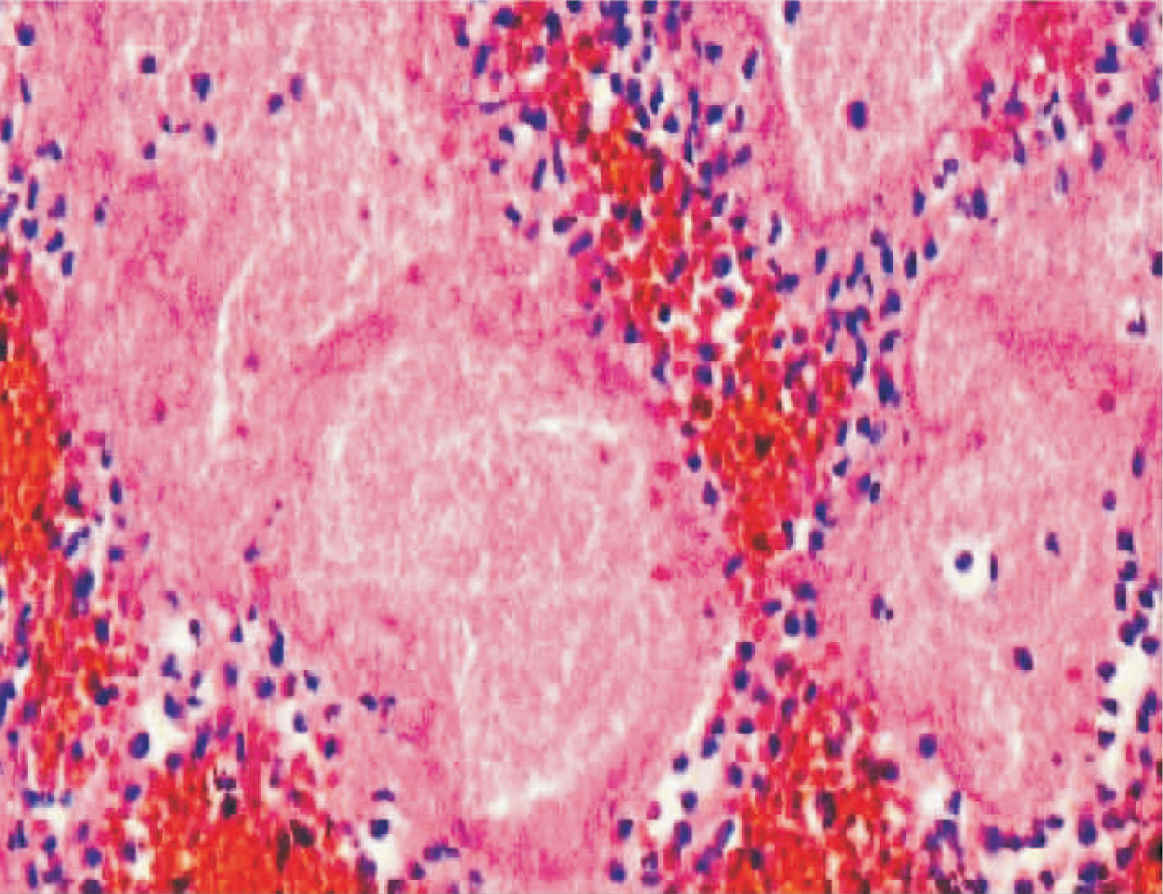
\includegraphics[width=.7\textwidth,height=\textheight,keepaspectratio]{./images/Image00040.jpg}
 \captionsetup{justification=centering}
 \caption{腔隙性脑梗死\\{\small A.病灶位于左侧基底节区和左侧额叶白质区;B.病灶位于脑干}}
 \label{fig2-22}
  \end{figure} 

\textbf{【鉴别诊断】}
脑腔隙在病理上为一脑实质内含水分的<15mm的潜在腔,包括穿支动脉等病变所致的腔隙性脑梗死和非血管病变引起的腔隙病变。发病机制包括血管因素所致的缺血即腔隙性梗死,以及血管因素(如出血、动脉炎等)和血管外因素(如炎症、变性、中毒、机械损伤等)所形成的腔隙性病变,应注意分析。此外,还应注意与前联合及基底节区的扩大的血管周围间隙(多在0.2~1.2cm大小)相鉴别,MR检查有独到鉴别价值。

\subsection{皮质下动脉硬化性脑病}

本病又称Binswanger病,是一组以脑深部小动脉硬化、痴呆、皮质下白质变性、皮质下腔隙或软化为特征的综合征。但有人认为“皮质下动脉硬化性脑病”一词未能正确反映所看到的组织学改变,且过高的估计了临床意义。因此,有关文献应用的非特异性名词较合适,如深部脑白质缺血或老年性白质高信号(MR)。我们认为称为“动脉硬化性脑白质病”或“深部脑白质慢性缺血”更趋合理,同时我们认为有关文献所述及的“脑白质疏松症”亦属本病的范畴。

\textbf{【病因病理】}
主要病因为慢性高血压,其病理特征为弥漫性不完全的皮质下梗死,在侧脑室旁和半卵圆中心的白质内髓鞘肿胀或脱失,皮质下弓状纤维与胼胝体不受累。常有皮质萎缩及皮质下、基底节区腔隙性脑梗死,在髓动脉内有狭窄性动脉粥样硬化。

\textbf{【临床表现】}
见于60岁以上老人,多隐形起病,呈进行性记忆力障碍、严重精神衰退、言语不清,反复发生的神经系统局部体征如偏瘫、失语、偏盲等。病情可缓解和反复加重,常伴有高血压。

\textbf{【CT表现】}
脑白质内斑片状或云絮状稍低密度灶,界限不清,其密度降低不如脑梗死明显。以侧脑室周围分布最明显,其次为半卵圆中心,多为两侧对称性(图\ref{fig2-23})。基底节---内囊区、丘脑、半卵圆中心常伴多发的腔隙性梗死灶,可有脑室系统扩大,脑沟、脑池增宽的弥漫性脑萎缩改变。

\begin{figure}[!htbp]
 \centering
 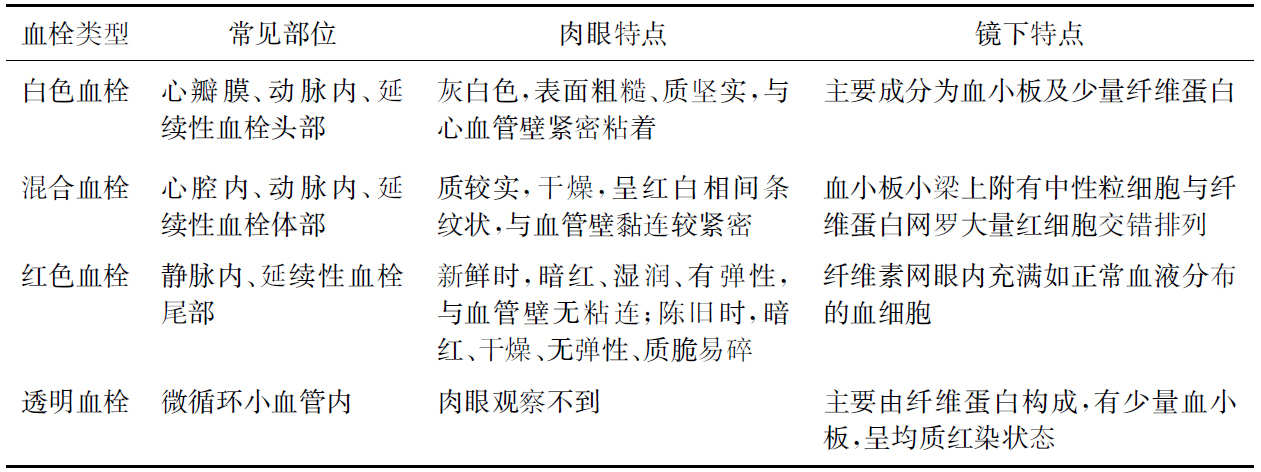
\includegraphics[width=.7\textwidth,height=\textheight,keepaspectratio]{./images/Image00041.jpg}
 \captionsetup{justification=centering}
 \caption{动脉硬化性脑白质病\\{\small 侧脑室周围白质和半卵圆中心区对称性片絮状低密度灶}}
 \label{fig2-23}
  \end{figure} 

\subsection{脑缺氧}

\textbf{【病因病理】}
脑缺氧包括乏氧性缺氧、血液性缺氧、循环性缺氧和中毒性缺氧。常见病因有:高空高原缺氧,呼吸功能不全和某些先心病循环短路、CO中毒以及各种严重贫血、各种休克和心衰,氰化物、硫化氢、磷中毒。脑组织局部循环性缺氧包括颅脑外伤、脑血管意外、脑血流障碍、颅内感染、脑肿瘤急性恶化等。主要病理改变为早期脑组织坏死、水肿,进行性脱髓鞘,晚期脑萎缩。

\textbf{【CT表现】}
①弥漫性脑水肿:以大脑为主,可出现大脑密度普遍减低,而丘脑、脑干和小脑密度相对较高的所谓CT反转征。②局部脑水肿:以脑动脉边缘带(分水岭区)、脑室周围白质最常见,基底节次之,也可见于丘脑和小脑。③缺氧性脑出血:脑实质、脑室周围-脑室、蛛网膜下腔、硬膜下或硬膜外。④脑萎缩:晚期可出现,也可见囊状软化灶。

\subsection{脑静脉窦血栓形成}

颅内静脉血流受阻即脑静脉和静脉窦血栓形成所导致的脑梗死称为静脉性脑梗死,占中风病人的1%~2%。

\textbf{【病因】}
近1/3病因不明。可分为:①全身因素:脱水、糖尿病、高凝血状态、血小板增多症、口服避孕药、妊娠、产后、近期手术、长期应用激素、肾病综合征、心脏病、结缔组织病、新生儿窒息等;②局部因素:局部感染、中耳乳突炎、鼻窦炎、脑膜炎、颅面中耳手术、颅脑外伤、动静脉畸形、动静脉瘘、腰穿等。

\textbf{【临床表现】}
多见于20~35岁女性,其表现各异。头痛最常见,15%急性起病,类似蛛网膜下腔出血,常伴头晕、恶心及视乳头水肿等颅内高压症状。1/3~1/2病人有局灶性神经症状,如颅神经麻痹和意识障碍,半数出现癫痫,还可有偏瘫。小脑静脉血栓可有共济失调等症状。

\textbf{【CT表现】}
最常见于上矢状窦、横窦和乙状窦,其次为海绵窦和直窦。特征性改变为致密静脉征(或索条征)和空三角征,但缺乏特异性。①早期(1~2天):平扫静脉窦内血栓密度与硬脑膜相似,可高达150Hu。增强扫描呈“空三角征”,即三角形的硬膜窦断面,中心不强化而周围强化。②第3~第10天:平扫窦内血块渐吸收,CT值约80Hu左右。③11天后:血凝块基本吸收,窦内CT值约50Hu。④静脉栓塞常伴有弥漫性非对称性脑肿胀、梗死性脑水肿、出血性梗死或单纯出血(脑实质和硬膜下)。静脉性出血其血肿周围界限不清,多靠近脑表面,而且周围环以大片低密度灶有别于动脉性出血。

\textbf{【鉴别诊断】}
高位分叉的上矢状窦、硬膜下脓肿和血肿、蛛网膜下腔出血及窦内窗孔和分隔均可类似空三角征;儿童的流动性静脉血常呈轻度高密度类似血栓,应注意鉴别。

\subsection{高血压脑病}

本病是指在血压迅速剧烈升高时,引起的急性全面性脑功能障碍,属可逆性后部白质脑病综合征(还见于妊娠高血压、慢性肾衰、使用免疫抑制剂和激素等)的范畴。

\textbf{【病因病理】}
可发生于各种原因(原发或继发)引起的动脉性高血压。病理上大多有不同程度的脑水肿,脑表面动脉、静脉和毛细血管扩张,脑切面可见斑点状、裂隙状出血和小动脉壁的坏死。

\textbf{【临床表现】}
该病一般起病急骤,病程短暂,所有症状历时数分钟或1~2小时,最多数天。主要表现为严重头痛、惊厥、偏瘫、失语、黑蒙、神志不清甚至昏迷。

\textbf{【CT表现】}
主要为广泛性脑水肿,呈对称性、弥漫性、边界不清的低密度区,以大脑半球后部最为显著,也可累及小脑。脑室系统变小,脑沟、脑池变浅。血压改善后一段时间随访,完全恢复正常。

\subsection{脑出血}

脑出血是指脑实质内的出血,又称为脑溢血或出血性脑卒中。

\textbf{【病因病理】}
其原因很多,临床上概括为损伤性和非损伤性两大类。后者又称为原发性或自发性脑出血,是指脑内血管病变、坏死、破裂而引起的出血。自发性脑出血绝大多数由高血压和动脉硬化(引起脑小动脉的微型动脉瘤或玻璃样变)所致,其次为脑血管畸形和动脉瘤所致。其他原因还有颅内肿瘤出血、出血性梗死、脑血管淀粉样变、全身出血性疾病、维生素缺乏、新生儿颅内出血、重症肝炎(可合并脑出血、梗死)等。

出血好发于壳核和内囊区(约占50%)、中心部脑白质、丘脑和下丘脑、小脑半球、桥脑,以及脑室内。病理可分为3期:①急性期:血肿内含新鲜血液或血块,周围脑组织有不同程度的水肿,还可有点状出血;②吸收期:血肿内红细胞破坏、血块液化,周围出现吞噬细胞,并逐渐形成含有丰富血管的肉芽组织;③囊变期:坏死组织被清除,缺损部分由胶质细胞及胶原纤维形成瘢痕,血肿小可由此类组织充填,血肿大时则遗留囊腔。

\textbf{【临床表现】}
本病常突然发生剧烈头痛、意识障碍、恶心、呕吐、偏瘫、失语、脑膜刺激征等,按病情发展可分为急性期、亚急性期和慢性期。

临床预后与出血的部位及出血量的多少有关。出血位于皮质下白质区,血肿及水肿引起占位效应,导致出血区功能丧失,但预后相对较好,出血量>30ml为手术指征。小脑或脑干出血压迫四脑室,继发急性颅内压升高,常伴延髓生命中枢损害,直接危及生命,血肿直径>3cm应立即手术。

\textbf{【CT表现】}
血液形成影像的主要成份为含铁的血红蛋白,血液的密度高于脑组织,故CT表现呈高密度。由于脑血管较细,受部分容积效应影响,故血管内血液多不能显示。严重贫血的患者急性期脑出血亦可呈等密度甚至低密度。

\subsubsection{出血量的估计}

一般采用以下公式计算:V(ml)=1/6
π(A×B×C),A为血肿前后径,B为左右径,C为上下径。A、B、C的单位均为厘米。

\subsubsection{CT分期}

通常将脑内血肿分为急性期(1周内)、吸收期(2周~2个月)和囊变期(2个月后)。也有学者根据密度分为:高密度期、等密度期、低密度期、慢性期(图\ref{fig2-24})。

\begin{figure}[!htbp]
 \centering
 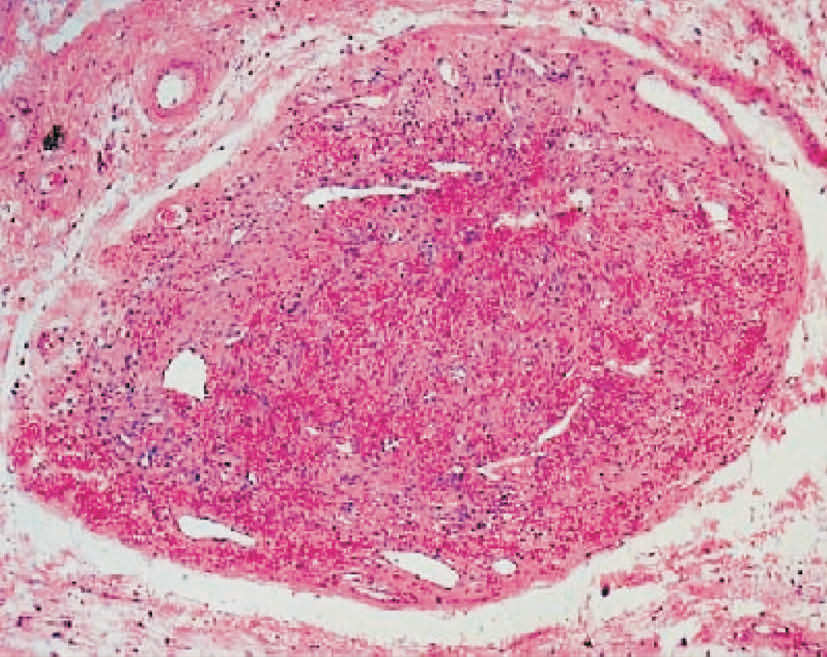
\includegraphics[width=.7\textwidth,height=\textheight,keepaspectratio]{./images/Image00042.jpg}
 \captionsetup{justification=centering}
 \caption{脑出血\\{\small A.右侧丘脑-外囊区血肿破入左右侧脑室内,右外侧裂内亦有血液充填;B.脑出血吸收期,血肿边缘开始吸收呈环状低密度,低密度外可见肉芽组织形成的等密度环}}
 \label{fig2-24}
  \end{figure} 

1.高密度期(1~14天):血液逸出血管后,红细胞分解释放含铁的血红蛋白,表现为高密度区,CT值约50~80Hu。出血3~4天因血液凝固成血块,血浆被吸收,红细胞压积增加,血肿密度达到高峰,甚者达90Hu,周围有水肿。严重贫血者可为等密度,甚至低密度,但血肿有占位征象。

2.等密度期(14~64天):血红蛋白分解,含铁血黄素开始被吸收,血肿呈等密度。但仍有占位效应,水肿仍存在,增强扫描呈环状强化。

3.低密度期(30~84天):血肿周围的新生血管及神经胶质增生形成血肿壁,血肿内含铁血黄素及血红蛋白被吸收,CT呈低密度灶。水肿消失,无占位效应,增强扫描仍呈环状强化。

4.慢性期(3个月后):少量脑出血被胶质和胶原纤维替代而愈合,CT呈略低密度灶。大量脑出血形成囊腔,CT近水样密度,并可出现牵拉现象,增强扫描无或轻微强化。

\subsubsection{脑室内出血}

单纯脑室出血与脑实质内出血破入脑室系统表现一样。少量出血时多沉积在侧脑室后角、第三脑室后部或第四脑室顶部,大量出血常呈脑室“铸型”样表现(图\ref{fig2-25})。早期可有分层现象,以后呈等或低密度,脑室内出血可形成脑积水。

\begin{figure}[!htbp]
 \centering
 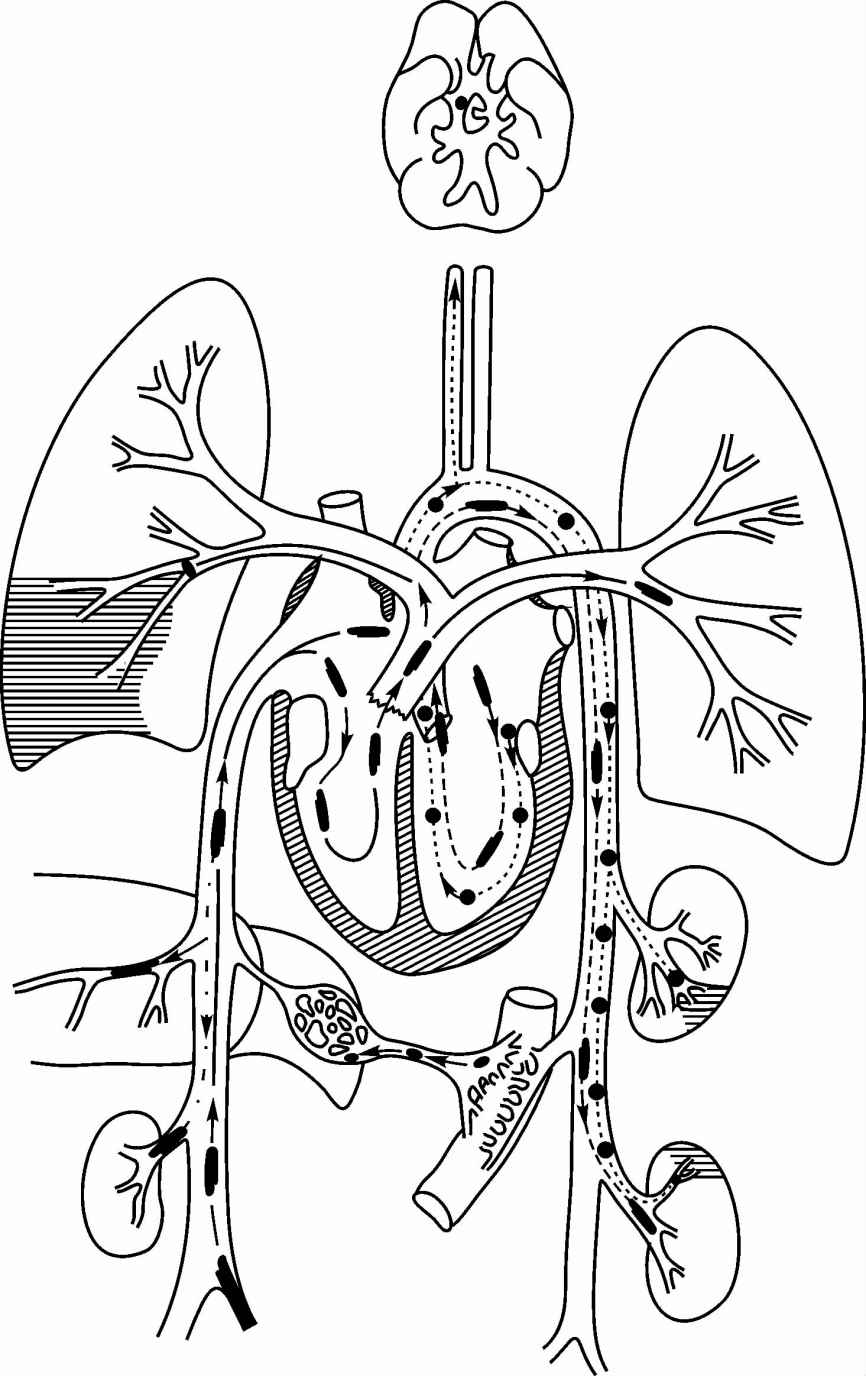
\includegraphics[width=.7\textwidth,height=\textheight,keepaspectratio]{./images/Image00043.jpg}
 \captionsetup{justification=centering}
 \caption{脑室内出血\\{\small 左右侧脑室内有大量血液充填,右侧呈“铸型”样表现}}
 \label{fig2-25}
  \end{figure} 

此外,在诊断时应注意:①急性脑出血大的血肿可形成脑疝。②脑出血可直接破入脑室系统和蛛网膜下腔,亦可由脑室系统进入蛛网膜下腔。③出血周围水肿,在第1天内可出现或表现轻微;3~7天达高峰;出血16天左右占位效应开始减退。④发现灶周水肿与血肿期龄不符时,应考虑肿瘤出血可能。⑤如局部伴有钙化或血肿密度不均等表现,除考虑到肿瘤出血外,也应考虑到脑血管畸形的可能。

\subsection{慢性扩展性脑内血肿}

本病是自发性脑内血肿的一种特殊类型,临床及影像学表现无特异性,易与肿瘤卒中、囊肿合并出血感染等混淆。

\textbf{【病因病理】}
其病因认为与隐匿性血管畸形、血管硬化、外伤、放射损伤、凝血功能障碍有关,一般没有高血压和脑外伤病史。隐匿性血管畸形或微小动脉瘤破裂出血,血肿及其代谢产物不断刺激周围组织产生炎性反应,毛细血管、纤维组织增生,并由增生的毛细血管、纤维组织形成包膜。而其丰富的毛细血管壁脆弱,反复出血、渗出,包膜内液化,使血肿体积逐渐增大。

\textbf{【CT表现】}
多为边缘清楚、密度均匀或不均匀的高、低混杂囊性病灶,且其内可见液-液平面。增强扫描病灶多无强化;部分血肿周围环状强化,为病灶周围脑组织或肉芽组织强化所致。

\subsection{蛛网膜下腔出血}

本病是指颅内血管破裂后血液注入蛛网膜下腔。

\textbf{【病因】}
临床可分为两大类,即外伤性与自发性。自发性原因很多,但以颅内动脉瘤(约占51%)、动静脉畸形(6%)和高血压动脉硬化所致(15%)最多见。此外,20%病因不明。

\textbf{【临床表现】}
自发性常有明显的诱因,如体力劳动过度、咳嗽、用力排便、情绪激动等。绝大多数起病急,剧烈头痛、呕吐、意识障碍、抽搐、脑膜刺激征等,同时可有偏瘫,腰穿有确诊价值。

\textbf{【CT表现】}
一般在出血3天内检出率最高,可达80%~100%,一周后很难检出。特征性表现为基底池、侧裂池和脑沟内等广泛的高密度影(图\ref{fig2-26})。如出血量少或严重贫血均不易发现。大脑前动脉破裂血液多积聚于视交叉池、纵裂前部;大脑中动脉破裂血液多积聚于一侧的外侧裂附近,也可向内流;颈内动脉破裂血液也以大脑外侧裂为多;椎基动脉破裂血液主要积聚于脚间池和环池。但出血量大者可难以估计出血部位。

\begin{figure}[!htbp]
 \centering
 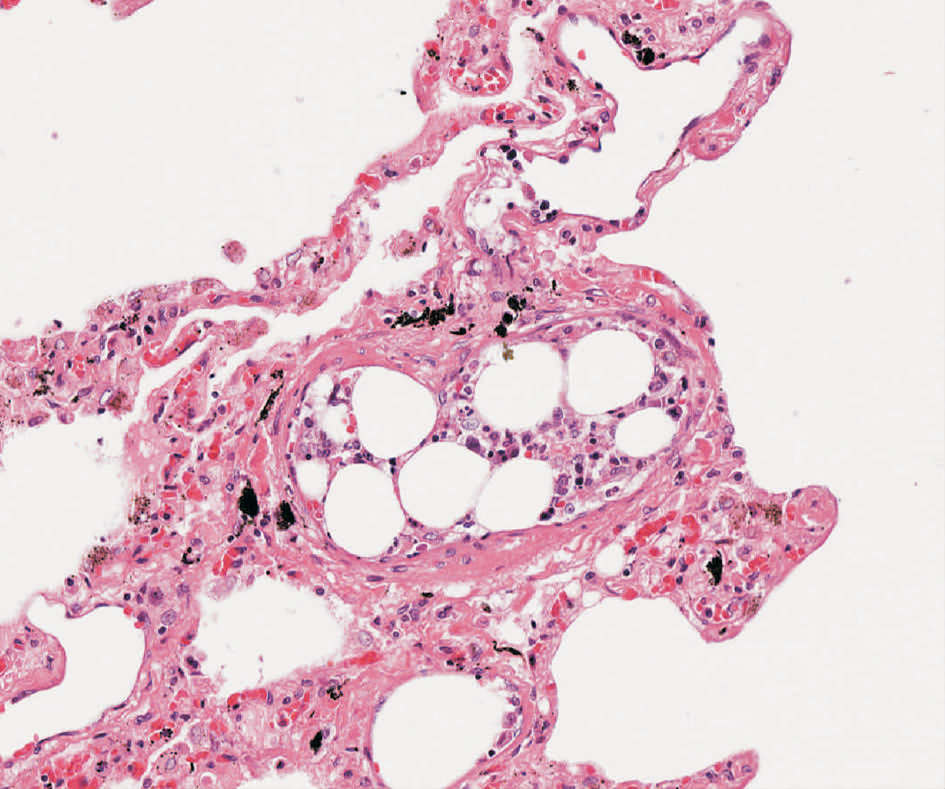
\includegraphics[width=.7\textwidth,height=\textheight,keepaspectratio]{./images/Image00044.jpg}
 \captionsetup{justification=centering}
 \caption{蛛网膜下腔出血\\{\small A、B为同一患者,鞍上池、左右外侧裂池、纵裂池前部、环池、四叠体池、大脑大静脉池内均有大量高密度血液充填}}
 \label{fig2-26}
  \end{figure} 

\textbf{【并发症】}
①脑积水:脑积水早期为梗阻性,发生率约为20%。可演变成交通性。②脑动脉痉挛:造成脑缺血和脑梗死,发生率约25%~42%。③伴发脑内血肿和(或)硬膜下血肿、脑室内出血:常与动脉瘤、动静脉畸形或脑肿瘤出血有关。

\subsection{颅内动脉瘤}

动脉壁呈局限性病理性扩张,与动脉腔有一颈部相连。

\textbf{【病因病理】}
其病因有先天性因素、动脉粥样硬化、感染因素和外伤4个方面。根据影像学可分为5种病理类型:①粟粒状动脉瘤;②囊状动脉瘤;③假性动脉瘤;④梭形动脉瘤;⑤壁间动脉瘤。

\textbf{【临床表现】}
好发于20~70岁。在破裂前90%无特殊临床症状,少数可影响到邻近神经或脑结构而产生症状。破裂后引起蛛网膜下腔出血和颅内血肿而出现相应的症状体征。

\textbf{【CT表现】}
颅内动脉瘤好发于脑动脉,约90%~95%分布于颈内动脉系统,5%~10%分布于椎动脉系统。颈内动脉瘤约占20%~40%,大脑中动脉瘤约占21%~31%,前交通及大脑前动脉瘤约占30%~37%,多发性约占4%~5%。

1.颅底较小动脉瘤:平扫难以显示,增强扫描呈高密度。

2.较大动脉瘤:平扫呈圆形等或高密度,边缘光整,有时瘤壁可见钙化。增强扫描呈均匀强化,而血栓无强化。

3.巨大动脉瘤:即直径>2.5cm的动脉瘤,其CT表现可分3型。①无血栓形成型:平扫呈圆形或椭圆形等或略高密度,瘤壁钙化较其他类型少见。增强扫描均匀强化。②部分血栓形成型:最常见,呈圆形或卵圆形略高密度,壁多有弧形钙化。增强扫描流动的血液强化明显,血栓不强化,从而形成高密度影内的低密度点称为“靶征”。周围很少有水肿。③完全栓塞型:平扫为圆形或卵圆形混杂略高密度,瘤壁常有钙化,周围无水肿。增强扫描呈环状强化。

此外,CTA显示动脉瘤的敏感性可达95%,特异性近83%。

\textbf{【并发症】}
①颅内出血:蛛网膜下腔出血、脑内血肿和脑室内积血,甚至可穿破蛛网膜造成硬膜下血肿。②脑血管痉挛:蛛网膜下腔出血所致,并导致相应区域的水肿、梗死。③脑积水:蛛网膜下腔出血所致。

\textbf{【鉴别诊断】}
动脉瘤周围多无水肿,瘤壁可有环形强化,动态CT扫描时间-密度曲线呈速生速降型,与血管相同。而肿瘤则表现为缓慢上升和下降的时间-密度曲线是鉴别的关键。

\subsection{脑动静脉畸形}

脑血管畸形分为5型:①动静脉畸形(AVM);②海绵状血管瘤;③静脉畸形(又称静脉血管瘤);④毛细血管扩张症(又称毛细血管瘤,以MR诊断为佳);⑤血管曲张(包括大脑大静脉畸形等)。其中AVM最常见,约占90%以上。毛细血管扩张症一般只被病理诊断,CT或MR很难显示,偶见钙化。

AVM是最常见的血管畸形,但有相当一部分脑血管造影阴性,称为隐匿性AVM。

\textbf{【病理】}
AVM由一条或多条供血动脉、畸形血管团、一条或多条引出静脉组成。常见于大脑中动脉分布区的脑皮质,亦可发生于侧脑室(如脉络丛)、硬脑膜、软脑膜、脑干和小脑。

\textbf{【临床表现】}
好发于20~30岁,男性多于女性,10%~15%无症状。常见的症状有:①头痛:偏头痛或全头痛,阵发性;②出血:出现相应症状和体征;③癫痫:约30%为此就诊;④脑缺血症状:脑梗死、脑萎缩;⑤部分颅外听到杂音。

\textbf{【CT表现】}
AVM平扫呈局灶性高、低或低、等混杂密度区,多呈团块状,也可见点、线状影,边缘不清,但有时可不显示。常伴斑点状或条状钙化,轻度或无占位征象。病灶周围无水肿表现,但有时可出现脑室扩大和交通性脑积水。增强扫描呈团块状强化,有时可见迂曲的血管影,造影剂充盈及排出均较快。CTA多可有效显示其供血动脉、畸形血管团和引流静脉(图\ref{fig2-27})。



\begin{figure}[!htbp]
 \centering
 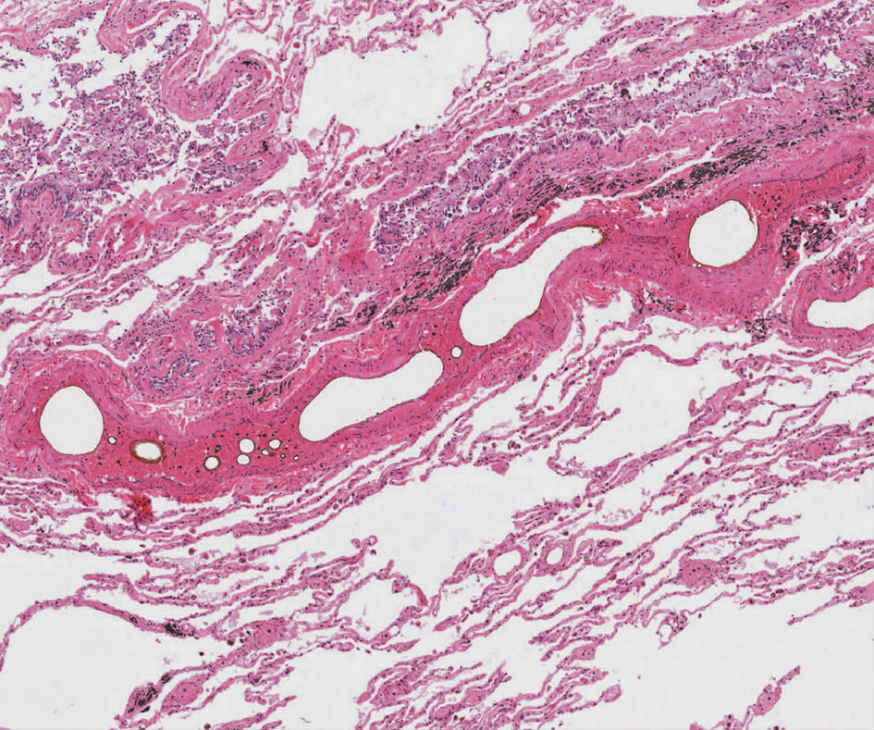
\includegraphics[width=\textwidth,height=\textheight,keepaspectratio]{./images/Image00045.jpg}
 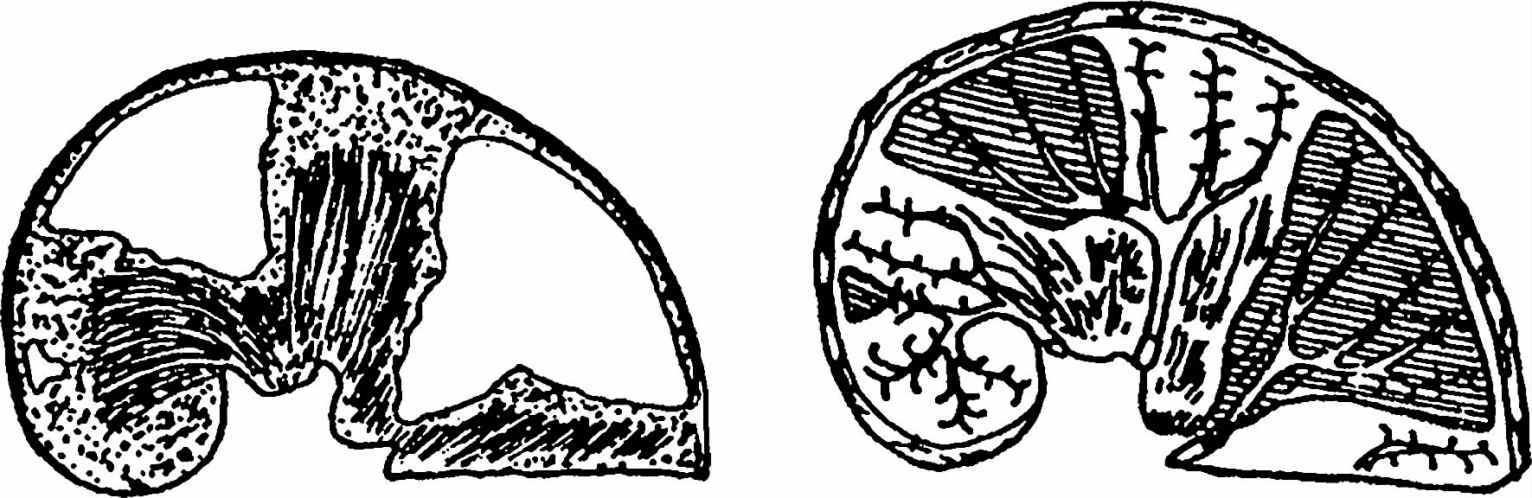
\includegraphics[width=\textwidth,height=\textheight,keepaspectratio]{./images/Image00046.jpg}
 \captionsetup{justification=centering}
 \caption{脑动静脉畸形\\{\small A~D为同一患者,平扫(A、B图)左侧颞叶有局灶性高、等混杂密度区,形态不规则,其边缘有蚯蚓状高密度影(引流静脉);增强扫描(C图)呈团块状强化,并见迂曲的引流静脉影;CTA(D图)清晰显示畸形血管团和粗大的引流静脉}}
 \label{fig2-27}
  \end{figure} 

其并发症有出血、梗死、软化灶及局限脑萎缩表现。

\textbf{【鉴别诊断】}
钙化明显的肿瘤以及强化明显的肿瘤(如胶质瘤)其水肿及占位效应均较显著,可与AVM鉴别。AVM增强扫描的时间-密度曲线与血管相似亦是与肿瘤鉴别的重要依据。

\subsection{颅内海绵状血管瘤}

本病占脑血管疾病的7%,近年来的研究显示其属不完全染色体显性遗传性疾病。目前多认为其发生源于脑内毛细血管水平的血管畸形,可位于脑内或脑外,为非真性肿瘤。

\textbf{【病理】}
病灶由微动脉延伸出来的、血流缓慢的、大小不等的丛状薄壁的血管窦样结构组成,其间有神经纤维分隔,窦间没有正常脑组织。由于其血管壁薄而缺乏弹性,且易于发生玻璃样变、纤维化,因而易出血,并可有胶质增生、坏死囊变、钙化,病灶可全部钙化形成“脑石”。病灶周围可见含铁血黄素沉着或有机化的血块。病灶无明显的供血动脉及引流静脉。

\textbf{【临床症状】}
好发于40~60岁,常以颅内出血为首发症状。典型表现为癫痫发作、突发性头痛和进行性神经功能障碍等。

\textbf{【CT表现】}
80%位于幕上,好发于额、颞叶,也可发生于蛛网膜下、硬膜下,脑外者多位于鞍旁海绵窦区。多表现为界限清楚的圆形或卵圆形的等至稍高密度影(图\ref{fig2-28})。其内可见“颗粒征”颇有特征,即在略高密度背景内含有数量不一的颗粒状高密度影和低密度影,前者为钙化,后者为血栓形成。除急性出血或较大病灶,灶周一般无水肿及占位征象。可能因为供血动脉太细或已有栓塞,也可能因病灶内血管床太大,血流缓慢使对比剂稀释,致使增强扫描不强化或仅见周边强化。其强化程度取决于病灶内血栓形成和钙化的程度,血栓形成轻、钙化不明显者强化明显。国外报道脑外者可有骨侵蚀。

\begin{figure}[!htbp]
 \centering
 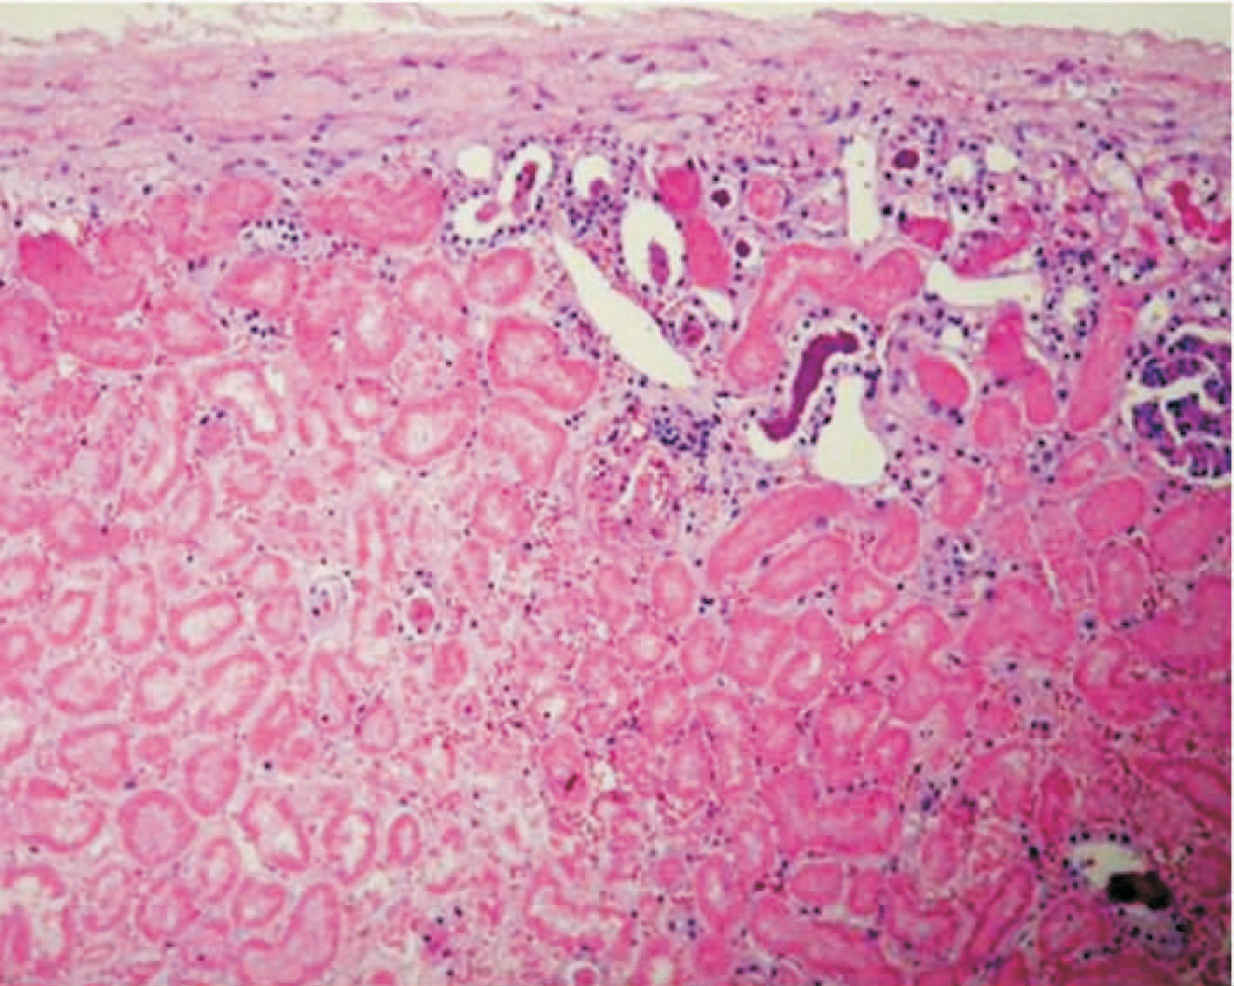
\includegraphics[width=.7\textwidth,height=\textheight,keepaspectratio]{./images/Image00047.jpg}
 \captionsetup{justification=centering}
 \caption{颅内海绵状血管瘤\\{\small A、B非同一患者,A示病灶位于小脑左侧半球,B示病灶位于脑干;病灶均呈近圆形稍高密度灶,周围无水肿}}
 \label{fig2-28}
  \end{figure} 

\textbf{【鉴别诊断】}
①主要应与脑膜瘤鉴别。后者平扫密度多均匀一致,增强扫描明显强化,常有明显占位征象,并可出现水肿征象及颅骨增生和吸收有助鉴别。②少数血管瘤呈环状并伴壁结节,偶有出血,病灶内显示血-液平面伴周围水肿,不易与胶质瘤等相鉴别。

\subsection{脑静脉性血管畸形}

本病又称脑静脉性血管瘤、脑发育性静脉异常,是一种组织学上由许多扩张的髓静脉和一条或多条引流静脉组成的血管畸形。国外有学者认为是一种正常引流静脉的非病理性变异。

\textbf{【病因病理】}
其病因不明,多认为是胚胎发育时宫内意外因素导致静脉阻塞,由侧支代偿所致。其形成时间在脑动脉形成之后,故仅含静脉成分。畸形血管由许多扩张的放射状排列的髓静脉汇入一条或多条引流静脉组成,向皮质表面和静脉窦或向室管膜下引流,可分为皮层表浅型、皮层下型和脑室旁型。

\textbf{【临床表现】}
好发于35~40岁,男女发病率相近。一般无症状,少数可产生癫痫、头痛,出血者可有感觉和运动障碍、共济失调等。

\textbf{【CT表现】}
它可发生在脑静脉系统的任何部位,但以额叶侧脑室前角附近的髓质区和小脑深部髓质区最常见,其次为顶叶、颞叶和脑干。

CT平扫阳性率不到50%。最常见的表现为圆形高密度影(34%),系扩张的髓静脉网,无水肿和占位效应,可见高密度的含铁血黄素沉着或钙化。

增强扫描阳性率为87%,可见3种表现:①白质中圆形强化影(32.5%),系髓静脉网或引流静脉;②穿越脑的线形增强影(32.5%),为引流静脉;③两者同时出现(18.6%)。

特征性表现是三维CT血管造影(CTA)静脉期脑静脉成像(CTV)出现“海蛇头”样的深部髓静脉汇集到单根粗大的引流静脉,然后汇入到表浅的表层静脉或硬膜窦等征象。但发生于脑室壁上者“海蛇头”征象不明显。

\subsection{Galen静脉瘤}

本病又称大脑大静脉扩张、大脑大静脉瘘、大脑大静脉畸形等。

\textbf{【病因病理】}
本病是由于动静脉短路,流入Galen静脉(即大脑大静脉)内的血流增多引起局部管腔扩张。这些短路血管多来源于颈内动脉系统或基底动脉系统,多异常扩大迂曲。静脉窦闭塞引起大脑大静脉回流受阻也是其重要的致病原因。压迫中脑导水管可致脑积水。

\textbf{【临床表现】}
在新生儿、幼儿中常因动脉血直接进入静脉造成心功能不全。脑积水后可出现头痛、痉挛性抽搐、颅内压增高等症状。

\textbf{【CT表现】}
平扫可见第三脑室后部中线处之大脑大静脉池区等密度或高密度的圆形肿块,病灶边缘多光滑,与窦汇之间有扩张的直窦相连为特异性表现。可伴有病灶边缘钙化、局部脑萎缩、血肿或脑积水。增强扫描病灶呈均匀性强化,偶可显示强化的供血动脉和引流静脉。

\subsection{颈动脉海绵窦瘘}

本病是指颈动脉及其分支与海绵窦之间异常沟通所致的一组临床综合征。海绵窦为中颅凹两层硬脑膜构成的硬脑膜窦,眼上静脉、眼下静脉、蝶顶窦静脉、外侧裂静脉和基底静脉汇入其中,颈动脉穿行其间。这是体内惟一动脉通过静脉的结构。当任何原因造成颈内动脉壁破裂后,动脉血直接流入海绵窦,就形成海绵窦区动静脉瘘。

\textbf{【病因】}
病因分为两大类:①外伤性:多见,大多由颅底骨折所致;②自发性:病因较多,主要见于颈内动脉虹吸部动脉瘤破裂、硬膜型动静脉畸形及遗传性胶原纤维缺乏病等。此外,动脉硬化、炎症、妊娠等也可造成自发性。根据解剖部位分为颈动脉海绵窦瘘和硬脑膜动脉海绵窦瘘,前者多为外伤性,后者多为自发性。

\textbf{【临床表现】}
头痛、癫痫、耳鸣、视力障碍、搏动性突眼、眼球运动障碍、颅内杂音,甚至因颅内出血而出现相应症状。

\textbf{【CT表现】}
①患侧海绵窦扩大,密度增高;②眼上静脉增粗;③眼球突出;④增强示扩大的海绵窦及迂曲的眼上静脉显著强化(图\ref{fig3-8},见第三章)。此外,眼外肌肥厚和眶内软组织肿胀、突眼,患侧脑组织水肿、出血、萎缩是引流静脉压力增高及“盗血”引起的继发改变。

\subsection{颅骨膜血窦}

本病又称血囊肿、局限性静脉曲张或骨血管瘤,是指紧贴颅骨外板的扩张静脉,它们穿过颅骨的板障静脉与硬膜窦相交通。

\textbf{【病因】}
其原因不明,可由先天性、自发性或外伤性所致。有学者认为外伤是本病的最主要因素。

\textbf{【临床表现】}
多见于儿童,通常以头皮肿块就诊。头皮中质软的膨隆性肿块,无搏动,局部皮肤可以微红或青紫色。通常位于中线部位,偶尔位于侧旁,以额部为主,偶有头痛、恶心、乏力等。肿块随颅内压力的变化而改变其大小,即平卧或头低时肿块增大为其特征性症状。

\textbf{【CT表现】}
大多位于颅外中线部位或附近,上矢状窦近端,以额、顶部多见。表现为颅外头皮下均匀的软组织密度肿块,边缘清晰,无钙化,随体位大小可变化。颅外板可有轻度压迹,颅骨内有孔状骨质缺损。增强扫描静脉窦内对比剂可通过颅骨的缺损弥散至囊腔内,呈均匀或不均匀显著强化。

\subsection{颅内血管延长症}

本病是指颈内动脉及椎基底动脉有规律的直径增大和普遍而有规律的延长为特征的血管异常。颈内动脉及椎基动脉的延长属于一种少见的先天性血管壁异常。

\textbf{【病理】}
延长的血管均伴有不同程度的动脉粥样硬化、弹性内膜的破坏及其肌壁的纤维化,最终导致血栓形成或栓塞。

\textbf{【临床表现】}
其发病特点主要取决于受累血管的范围、病变大小及所压迫的邻近组织情况。基本分为3类:①脑血管意外;②颅神经受压症状:如Ⅲ、Ⅴ~Ⅷ颅神经受压;③占位效应对脑组织功能的影响:如痴呆、共济失调、震颤麻痹等,也有阻塞性脑积水的可能。

\textbf{【CT表现】}
本病所涉及的血管有基底动脉、颈内动脉幕上段、大脑中动脉、大脑后动脉。CTA可发现异常扭曲扩张的颈内或基底动脉段,管壁可钙化。其中,基底动脉病变的诊断标准为上段基底动脉的直径增大达4.5mm和基底动脉上段超过床突平面6mm以上,且延长的血管可伴有迂曲移位和血管袢形成。

\subsection{烟雾病}

本病又称Moyamoya病、脑底动脉环闭塞、脑底异常血管网症等,是一种脑动脉进行性狭窄、闭塞性疾病。

\textbf{【病因】}
其病因不明,凡能引起颈内动脉末端、大脑前动脉和大脑中动脉近端慢性进行性闭塞的先天因素(发育不良)或后天因素(外伤、感染、动脉硬化)均可导致本病。近来遗传因素受到重视。

\textbf{【临床表现】}
以10岁以前儿童多见,亦可见于成人。主要有缺血性和出血性两大类表现。脑血管造影是确诊的主要手段。

\textbf{【血管造影】}
特点为:①大脑前、中动脉起始处狭窄或闭塞;②脑底异常血管网形成;③侧支循环广泛建立;④两侧颞、额、顶叶、基底节区梗死或出血。本病即因造影时异常血管网和侧支循环的显影似烟雾状而得名。

\textbf{【CT表现】}
无特异性。①脑梗死、软化灶:常见于颞、额、顶叶,很少见于基底节,小脑、脑干不发生。②脑萎缩:多为双侧性,额叶为甚,脑室扩大以侧脑室和第三脑室显著。③出血灶:可为脑内或蛛网膜下腔。④颅底、基底节区有点状、迂曲、不规则的网状影,并可见强化。

\section{颅脑外伤及其他损害}

\subsection{头皮损伤}

颅盖软组织在额、顶、枕部分为皮肤、皮下组织、帽状腱膜、帽状腱膜下层和颅骨骨膜5层。前3层紧密连接CT不能识别。帽状腱膜下层由疏松结缔组织构成,内含少量血管,CT呈低密度带。而在颞部则由皮肤、皮下组织、颞浅筋膜、颞深筋膜、颞肌和颅骨骨膜6层构成。

头皮损伤包括:①头皮血肿或称颅外血肿,包括位于头皮与帽状腱膜间的皮下血肿、帽状腱膜下血肿(图\ref{fig2-29})和骨膜下血肿;②头皮撕裂伤、擦伤和挫伤等。

\begin{figure}[!htbp]
 \centering
 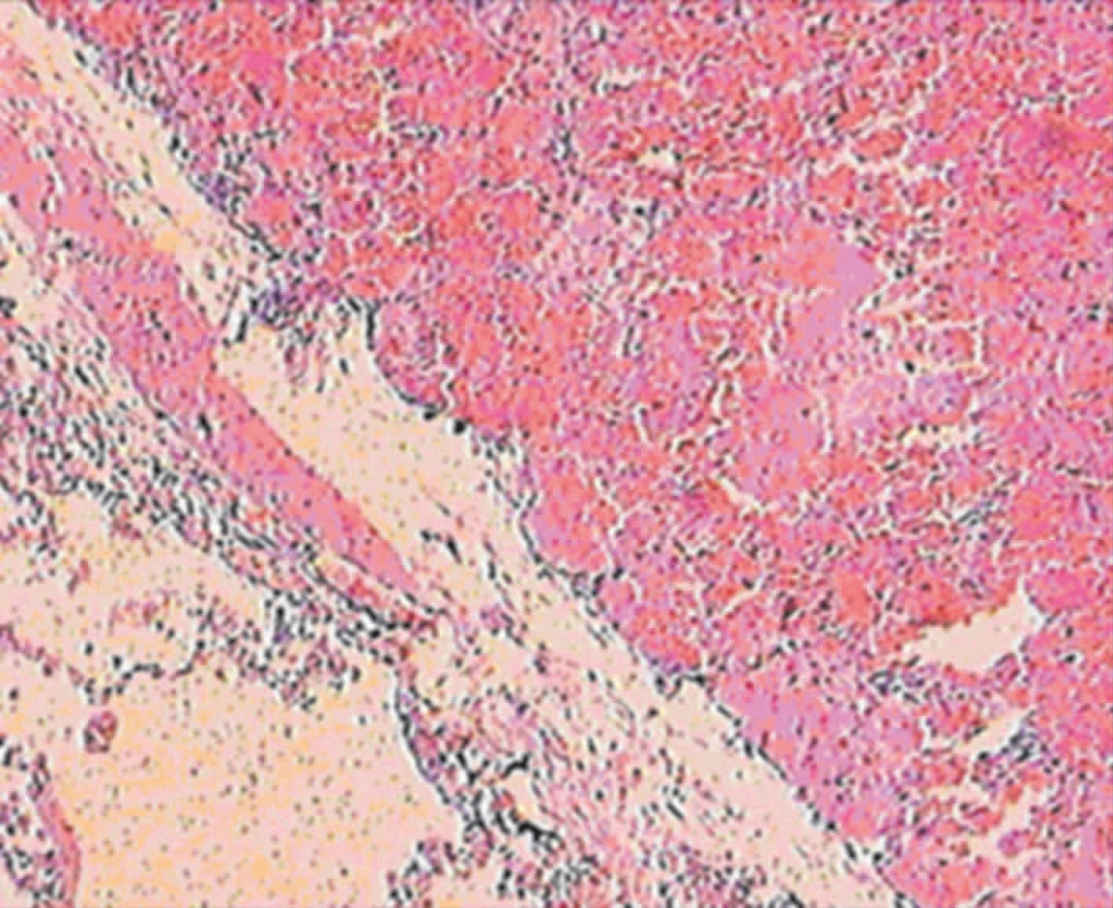
\includegraphics[width=.7\textwidth,height=\textheight,keepaspectratio]{./images/Image00048.jpg}
 \captionsetup{justification=centering}
 \caption{帽状腱膜下血肿\\{\small 出血位于左侧额顶枕部帽状腱膜下}}
 \label{fig2-29}
  \end{figure} 

头皮血肿多由于头皮血管破裂引起,也可因板障静脉或硬脑膜血管破裂,血液沿骨折缝聚集于骨膜下,后者多伴硬膜外血肿。

\subsection{颅骨骨膜下血肿}

骨膜下血肿是颅外血肿的少见类型。

\textbf{【病因病理】}
多发生于新生儿产伤和婴幼儿头部外伤。血肿位于颅骨外板与对应的骨膜之间的潜在腔隙,好发于顶骨,其次为枕骨。

\textbf{【临床表现】}
产伤所致者几乎均因头皮下出现软组织包块,未消散且逐渐变硬而就诊。

\textbf{【CT表现】}
特征性表现是新鲜血肿范围达到受累骨的整个表面,中止于颅缝或不跨越颅缝,边缘清楚锐利。而头皮下及帽状腱膜下血肿不受颅缝限制有助于鉴别。2~3周后血肿包膜出现弧形、壳状钙化,从边缘开始逐渐形成一个完整的包壳,这一过程大约需要3~6个月。与此同时血肿逐渐吸收机化,血肿完全机化约需1年,此时血肿包膜钙化或骨化形似颅骨外板,血肿机化钙化形似板障。再经过长期的塑形与颅骨融合,致局部颅骨增厚、外突隆起,并可成为永久性后遗表现。

此外,少数在血肿部位出现或大或小的囊状骨缺损,可持续数年或更久。与颅骨表皮样囊肿、嗜酸性肉芽肿、韩雪柯氏病相类似,应注意鉴别。

\subsection{颅骨骨折}

1.按骨折形态分类:①线状骨折。②凹陷骨折:婴幼儿颅骨质软,骨折部位凹陷,但不出现骨折线,称为乒乓球样凹陷骨折。③粉碎性骨折:大多数凹陷骨折被分离为多个骨碎块,则被称为粉碎性骨折。④穿通骨折:多为锐器直接损伤,少数为火器伤。局部头皮全层裂伤,可有各种类型骨折,还可见颅内血肿、异物及脑损伤。⑤颅缝分离:两侧不对称或颅缝宽>2mm。

2.按骨折部位分类:①颅盖骨骨折。②颅底骨折。

3.诊断骨折应注意的问题:①颅骨血管沟:仅有内板压迹,边缘为硬化边。②板障静脉:常不规则,可见于对侧,并终端于静脉湖。③颅骨缝:特有的部位及走行,是区别骨折线的标志。④是否有颅内积气:积气可见于蛛网膜下腔、脑室系统、硬膜下腔,以及硬膜外血肿内,甚至脑实质内。

\subsection{硬脑膜外血肿}

硬脑膜紧贴颅骨内板,当颅骨骨折或脑膜血管破裂、出血使其与颅内板分离时则形成硬膜外血肿。

\textbf{【病理】} 多发生于头颅直接损伤的部位。约
95%伴颅骨骨折,70%~80%病例因骨折所致脑膜中动脉及其分支断裂,少数因骨折伤及板障静脉、静脉窦和蛛网膜粒。血肿可单发或多发,呈凸透镜形,多不伴有脑实质损伤。

\textbf{【临床表现】}
伤后有短时原发昏迷,清醒后头痛、呕吐逐渐加重并再度昏迷。清醒时间的长短,由出血量多少和出血速度决定。重者如不及时处理,可形成脑疝。

\textbf{【CT表现】}
因硬膜与颅骨紧密相连,故血肿局限呈梭形高密度,CT值为50~70Hu。血肿的脑侧缘光滑(图\ref{fig2-30}),好发于骨折处。由于硬膜在颅缝处与骨结合紧密,故血肿不超越颅缝。但骨折如跨越颅缝,则血肿亦可跨越颅缝,也可从幕上延及幕下或跨越中线。血肿有占位效应,但较硬膜下血肿轻,多不伴脑实质损伤,但压迫邻近血管时可发生脑水肿或脑梗死。少数受伤时无症状,以后才发生慢性硬膜外血肿。慢性硬膜外血肿其壁机化增厚并可钙化。

\begin{figure}[!htbp]
 \centering
 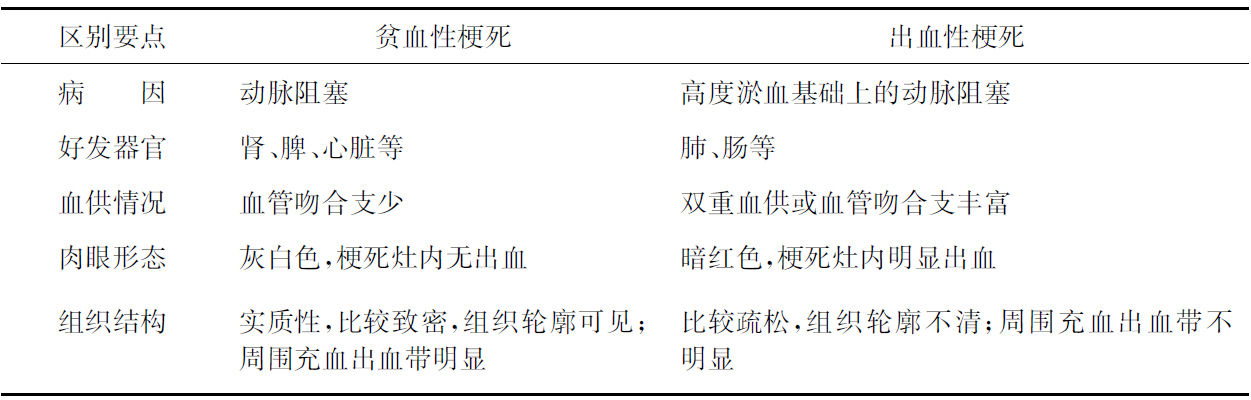
\includegraphics[width=.7\textwidth,height=\textheight,keepaspectratio]{./images/Image00049.jpg}
 \captionsetup{justification=centering}
 \caption{硬膜外血肿\\{\small 右侧颅骨内板下有梭形高密度区,边缘清晰锐利}}
 \label{fig2-30}
  \end{figure} 

\subsection{硬脑膜下血肿}

硬膜下血肿位于硬膜和蛛网膜之间,多因减速性挫伤(对冲伤)所致,无颅骨骨折或骨折仅位于暴力部位。

\textbf{【病理】}
其血源多为脑对冲伤处的静脉、小动脉或由大脑向上矢状窦汇入的桥静脉撕裂所致。呈新月形包绕在大脑表面,在伤后不同时间形态变化各异,约50%合并脑挫裂伤。临床、病理和影像均分为急性、亚急性和慢性3期。

CT上等密度硬膜下血肿占硬膜下血肿的16%。据有关文献报道,多发生在初次损伤后30~90天,亦有报道可达120天,甚至150余天。等密度硬膜下血肿的原因为:①血肿由高密度向低密度发展过程中血肿密度与脑组织密度相近时;②偶有低蛋白血症(如贫血)病人的急性期血肿呈等密度;③再出血或慢性出血进入到慢性硬膜下血肿,而形成等密度慢性硬膜下血肿。

\textbf{【临床表现】}
急性者病情多较重,且发展迅速,出现中间清醒期或意识好转期者较少,颅内压增高、脑受压和脑疝症状出现早。慢性硬膜下血肿患者年龄常较大,只有轻微外伤史,在伤后数周或数月出现颅内压增高症状,呈慢性过程。

\textbf{【CT表现】}

\subsubsection{三期表现}

1.急性期:伤后3天内。一般呈均匀高密度的新月形(图\ref{fig2-31}A),血肿可跨颅缝,但不超过中线。占位效应著,常伴脑挫裂伤,可形成脑疝。有3种非典型表现:①血肿密度不均:可能与急性出血还未凝固、凝血早期血清外溢或蛛网膜破裂脑脊液进入硬膜下有关;②血肿呈梭形表现:可能与出血没有及时散开有关;③血肿同侧侧脑室扩大:可能与同侧室间孔被迅速挤压梗阻所致。

此外,多不伴骨折,但骨折后硬膜撕裂也可形成急性硬膜下血肿。

2.亚急性期:伤后4天~3周内。血肿可逐渐变为等密度,而表现为皮质区均匀受压,脑沟消失,灰白质交界处被均匀向内推移。但双侧均有血肿,中线推移可不著。亚急性血肿的较早期出现细胞沉淀效应可出现密度上低下高的液体界面。

3.慢性期:伤3周后。此时血肿包膜形成,凝血块液化,逐渐变成液性低密度(图\ref{fig2-31}B),血肿壁机化增厚或钙化。血肿内肉芽组织增生、机化形成包膜,故可见慢性硬膜下血肿有分隔表现。

\subsubsection{等密度硬膜下血肿}

平扫表现为中线结构及脑室受压移位、变形,脑沟、裂池变窄消失、灰白质界面内移等,均属间接征象(图\ref{fig2-31}C)。增强扫描可显示血肿的位置、大小、形态而确诊。



\begin{figure}[!htbp]
 \centering
 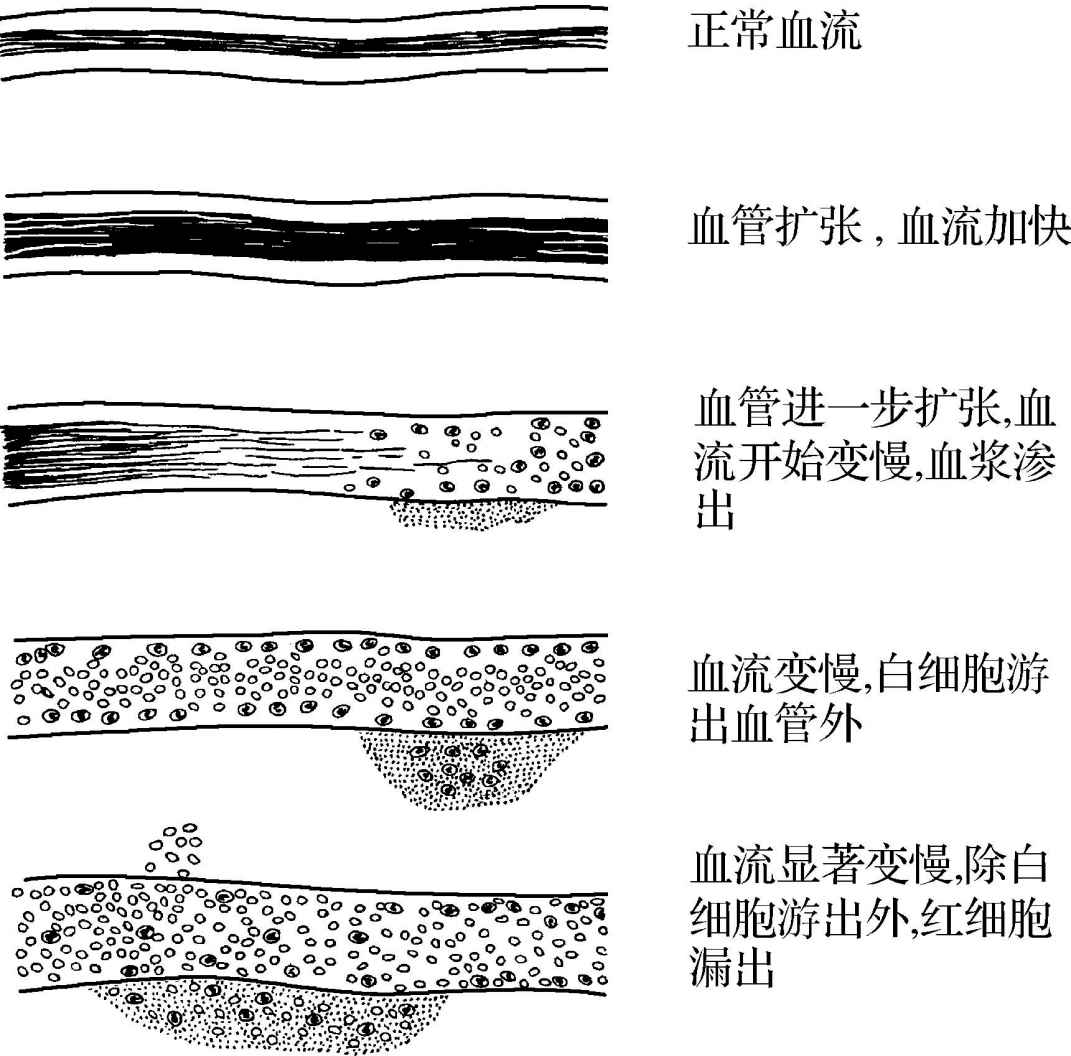
\includegraphics[width=.7\textwidth,height=\textheight,keepaspectratio]{./images/Image00050.jpg}
 \includegraphics[width=.7\textwidth,height=\textheight,keepaspectratio]{./images/Image00051.jpg}
 \captionsetup{justification=centering}
 \caption{硬膜下血肿\\{\small A.急性期硬膜下血肿,病灶位于左侧额顶骨内板下;B.慢性期硬膜下血肿,病灶位于左侧额顶枕骨内板下,有密度上低下高的液体界面;C.慢性等密度硬膜下血肿,病灶位于左侧额顶枕骨内板下和右侧额部}}
 \label{fig2-31}
  \end{figure} 

\subsection{特殊部位的硬脑膜下血肿}

特殊部位的硬膜下血肿主要指大脑镰、小脑幕硬膜下血肿。

\textbf{【病因病理】}
其受力方式可以是加速运动或减速运动的直接作用力,也可以是引起大脑镰、小脑幕严重移位的内在推力。目前,普遍认为是该处的桥静脉与静脉窦连接部撕裂,血液进入硬膜下腔所致。

\textbf{【CT表现】}

1.大脑镰硬膜下血肿:正常大脑镰宽为<3mm,硬膜下血肿表现为大脑纵裂呈带状增宽,密度增高,宽为3~12mm,CT值达68~85Hu,可有占位效应。硬膜侧有坚硬的硬膜阻挡,故其内缘平直而光整;外缘因蛛网膜的张力低和脑沟、脑回的阻力不均衡呈局限的弧形或波浪状。但与脑沟不通为其特点,并可依此与蛛网膜下腔出血相鉴别(图\ref{fig2-32}A、B)。

2.小脑幕硬膜下血肿:呈扇形、片状、新月形等形状的高密度,内缘止于小脑幕切迹处。边缘光滑锐利,占位效应不著(图\ref{fig2-32}C、D)。由于小脑幕凹面向下,横断扫描像一般显示:血肿位于小脑幕上者,其内侧缘清晰,外侧缘模糊;位于小脑幕下者反之。



\begin{figure}[!htbp]
 \centering
 \includegraphics[width=\textwidth,height=\textheight,keepaspectratio]{./images/Image00052.jpg}
 \includegraphics[width=\textwidth,height=\textheight,keepaspectratio]{./images/Image00053.jpg}
 \captionsetup{justification=centering}
 \caption{特殊部位硬膜下血肿\\{\small A~D为同一患者;A、B血肿位于大脑镰旁,大脑纵裂呈带状增宽,边缘清晰、平直而光整;C、D血肿位于右侧小脑幕处,呈扇形高密度,内缘止于小脑幕切迹处,边缘光滑锐利}}
 \label{fig2-32}
  \end{figure} 

以上两者均可因部分容积效应或同时合并该区域的蛛网膜下腔出血而使血肿边界不清。

\textbf{【鉴别诊断】}
大脑镰旁和小脑幕处的硬膜下血肿主要应与蛛网膜下腔出血相鉴别。①前者边界光整清楚;后者则模糊不规则,因向脑沟延伸而多呈羽毛状,常波及相邻脑池和脑室。②前者大脑镰部占位效应常见;后者较少见。③前者血肿不能触及胼胝体膝部;后者可紧贴。④前者急性期密度多为55~75Hu,多在2周后吸收或变为低密度;后者CT值多在55Hu以下,且多在1周内(甚至24h)消失。⑤采用薄层扫描,特别冠状和矢状面重建可较清楚显示血肿的形态和解剖位置。此外,脑膜钙化CT值明显高于血肿可资鉴别。

\subsection{硬脑膜下积液}

本病又称硬膜下水瘤,是指硬膜下只含有脑脊液成分。

\textbf{【病因病理】}
它是由于外伤后蛛网膜破裂,脑脊液流入硬膜下所造成的,并多认为其形成机制是蛛网膜破口的活瓣效应的结果。常在外伤后几周内产生,少数因伴有慢性渗血而转化为慢性硬膜下血肿。

\textbf{【临床表现】}
多见于老年人及儿童。急性者(伤后72小时内)与急性颅内血肿症状相似,主要表现为头痛、恶心、呕吐等颅内压增高症状,亦可有局部脑受压症状。慢性者(3周后)可见嗜睡、朦胧、定向力差、精神障碍。

\textbf{【CT表现】}
多位于额、颞部,老年人双侧多见。呈颅骨内板下新月形水样密度区,因受压脑沟变浅、脑回变平(图\ref{fig2-33})。少数经复查液体密度增高,而转化为等密度或稍低密度慢性硬膜下血肿。

\begin{figure}[!htbp]
 \centering
 \includegraphics[width=.7\textwidth,height=\textheight,keepaspectratio]{./images/Image00054.jpg}
 \captionsetup{justification=centering}
 \caption{硬膜下积液\\{\small 双侧额颞骨内板下新月形水样密度区,脑沟变浅、脑回变平}}
 \label{fig2-33}
  \end{figure} 

\textbf{【鉴别诊断】}
①慢性硬膜下血肿:有人认为硬膜下血肿吸收后也可称为硬膜下积液。但慢性血肿CT值偏高,包膜有强化,常呈梭形,可予鉴别。②脑萎缩:脑沟裂增深、增宽,甚至脑室扩大等有别于硬膜下积液之脑沟、回变浅平。

\subsection{外伤性蛛网膜下腔出血}

\textbf{【病因病理】}
出血来源于外伤后软脑膜和皮层血管的断裂、脑挫裂伤的渗血及脑内血肿破入。单独蛛网膜下腔出血少见,多伴脑挫裂伤。

\textbf{【临床表现】}
因脑膜刺激引起剧烈头痛、恶心呕吐,查体可发现颈强直、Kernig征阳性。

\textbf{【CT表现】}
高密度血液充填于脑表面脑沟中或脑裂、脑池中。吸收消散快,长者1周,短者1~2天,最快可达10小时左右。可伴脑挫裂伤的水肿、出血等表现。

此外,少数(包括自发性)出血点因远离宽大的脑池、脑裂,而且出血较快,局限于局部颅骨内板下,与硬膜下血肿相似,但其内缘不锐利、密度较低且不均匀,且短期内能快速吸收。

\subsection{外伤性脑室内出血}

本病是一种较少见的重型脑损伤,预后差,死亡率高。

\textbf{【病因病理】}
本病可分为两类:①原发性:为外伤致脑室内血管破裂出血;②继发性:为脑内血肿破入脑室。其发生机理有以下几种学说:①脑外伤瞬间,外力(尤其矢状方向外力)使脑室扩大变形,撕裂室管膜下血管引起脑室出血。②弥漫性轴索损伤,由于剪切力的作用脑室壁破裂,引起室管膜下血管损伤出血。③室管膜下潜在的畸形血管破裂出血。④凝血功能障碍,外伤作为诱因。⑤脑内血肿破入脑室。

\textbf{【临床表现】}
多伴有其他类型的脑损伤,故缺乏特征性。可有以下表现:①意识障碍;②脑膜刺激征:脑室内出血流入蛛网膜下腔所致;③体温升高:是血性脑脊液的吸收热,并与出血刺激丘脑下部体温调节中枢有关。伴有其他部位的损伤时有相应表现和体征。

\textbf{【CT表现】}
少量出血时多沉积在侧脑室后角、第三脑室后部或第四脑室顶部,大量出血常呈脑室“铸型”样表现。早期可有分层现象,以后呈等或低密度。可并发不同程度的阻塞性脑积水,多合并其他类型脑损伤。

\subsection{脑挫裂伤}

脑组织外伤后发生水肿、静脉淤血、渗血及毛细血管的散在点状出血,病理上称为脑挫伤;而当软脑膜和脑组织及其血管断裂时称为脑裂伤。因而两者多合并存在,且临床和影像检查难以区分,故统称为脑挫裂伤。

\textbf{【病因病理】}
直接打击的外力可造成受力处的脑挫裂伤,此种较少。多由于运动中的撞击造成的对冲伤引起。病理改变有局部脑水肿,静脉淤血、渗血及毛细血管的散在点状出血,严重者出血较多,形成脑内血肿,还可有坏死液化等改变。

\textbf{【临床表现】}
都有意识丧失,出现一过性昏迷,重者持续昏迷。患者有头痛、呕吐等颅内压升高或脑膜刺激征。损伤部位不同可出现偏瘫、偏盲、肢体张力和腱反射的异常。

\textbf{【CT表现】}

1.常见表现:①局部脑组织呈低密度水肿,界限不清,多位于皮层区。水肿区内有一处或多处点片状出血灶称为灶状出血。②一处或多处脑内血肿(出血灶>2cm称为血肿),形态边缘不规整(图\ref{fig2-34})。血肿周围有不同程度水肿和占位效应。③灶状出血及小血肿可在数小时内扩大融合,并可引起脑疝如镰下疝、天幕疝等。

\begin{figure}[!htbp]
 \centering
 \includegraphics[width=.7\textwidth,height=\textheight,keepaspectratio]{./images/Image00055.jpg}
 \captionsetup{justification=centering}
 \caption{脑挫裂伤\\{\small 双侧额颞叶有许多斑片状不规则出血灶,鞍上池、四叠体池内有积血}}
 \label{fig2-34}
  \end{figure} 

2.外伤性迟发性脑内血肿:伤后首诊CT扫描未发现血肿,相隔数小时、数天复查或手术发现有新的血肿者称为外伤性迟发性脑内血肿。属于原发性脑损伤,可发生于伤后1.5小时至数天,90%以上出现在伤后24~48小时,也有报道多见于3日至1周内。此外,颅脑损伤的迟发性表现还有脑挫裂伤、硬膜外血肿、硬膜下血肿、蛛网膜下腔出血、脑水肿等。

3.其他伴发的外伤性颅内病变:硬膜外或硬膜下血肿、蛛网膜下腔出血、弥漫性脑水肿、硬膜下积液、DAI等。

\subsection{脑干损伤}

脑干损伤较少,多合并大脑半球的弥漫性损伤。

\textbf{【病理】}
本病可分为原发性和继发性。原发性病理改变有脑干震荡、挫裂伤、出血、软化和水肿。有人把其分为4类:①弥漫性轴索损伤(DAI);②原发性多发斑点状出血;③桥脑、延髓撕裂;④直接表浅撕裂或挫伤。其中以DAI最常见,且多为非出血性。继发性脑干损伤是由颅内血肿、脑水肿所致的天幕裂孔疝压迫脑干并使脑干血管受牵拉,进而导致脑干缺血和出血。

\textbf{【临床表现】}
病情严重,常见表现有意识障碍、去大脑强直、肌张力增高和眼球位置异常。患者常见双侧瞳孔缩小。

\textbf{【CT表现】}
因受后颅窝伪影干扰和分辨率限制对非出血性脑干损伤诊断困难。①原发性:常表现为局部脑池消失,亦可显示小灶状出血。②继发性:可见出血、梗死,并可见幕上血肿、弥漫性脑肿胀、弥漫性脑水肿、天幕裂孔疝和脑干受压移位等表现。

\subsection{弥漫性脑损伤}

弥漫性脑损伤包括弥漫性脑水肿、弥漫性脑肿胀和弥漫性轴索损伤(DAI)。弥漫性轴索损伤有文献也称为弥漫性脑白质损伤。

\textbf{【病因病理】}
DAI是因外伤造成的剪切力(旋转暴力)作用于脑灰白质交界处、大脑深部结构和脑干区,导致神经轴索的广泛挫伤、断裂及脑组织小灶出血、水肿。

脑水肿和脑肿胀的病理改变分别为细胞外液和细胞内液增多。两者常同时存在,很难区分和鉴别,因此统称为脑水肿(脑组织液体含量增多引起的脑容积增大和重量增加)。

\textbf{【临床表现】}
脑水肿和脑肿胀轻者无明显症状和体征,重者出现头痛、头晕、呕吐等颅内高压征;可出现半身轻瘫和锥体束征;严重者可发生脑疝,以至死亡。

DAI因广泛轴索损伤使皮层及皮层下中枢失去联系而致伤后即刻意识丧失,多持久昏迷,甚至处于植物人状态,死亡率高。

\textbf{【影像学表现】}

1.弥漫性脑水肿和(或)脑肿胀:CT表现为低密度,密度低于邻近脑白质,CT值多<20Hu。两侧弥漫性病变可致脑室普遍受压变小,重者可致脑室、脑沟和脑池消失。

2.DAI的诊断标准:①受伤机制:受伤时头部处于运动状态,由旋转暴力所致。②临床表现:伤后有原发性昏迷伴躁动不安,无明确神经定位体征,亦无窒息及低血压等脑缺氧情况。③CT表现:脑组织弥漫性肿胀(灰白质密度普遍降低,但其密度减低不及脑水肿),灰白质分界不清,其交界处有散在斑点状出血灶(<2cm),伴有蛛网膜下腔出血。脑室、脑池受压变小,无局部占位征象。④MR表现:脑肿胀、脑室脑池因受压而减小或闭塞,脑白质及胼胝体、脑干、小脑可见点状、片状或散在小出血灶(<2cm),中线结构无明显移位。⑤合并症:可合并其他颅脑损伤,如蛛网膜下腔出血、脑室出血、硬膜下及硬膜外血肿及颅骨骨折等。

DAT的分期:目前有学者将DAI分为3期。Ⅰ期:较轻,损伤仅见脑叶白质,常见于额、颞叶。Ⅱ期:损伤较重,胼胝体出现病灶。Ⅲ期:严重损伤,脑干出现病灶。

总之,因DAI有80%为非出血性病灶,仅20%有小的中心出血,故CT难以发现。其CT检出率不到30%,而MR可高达90%。

\subsection{外伤性脑疝}

\subsubsection{天幕疝}

分为3型:①颞叶型:常为单侧,占位效应显著,颞叶组织(钩回、海马回)疝入幕下;②中央型:常为双侧颅内压升高,脑干向下移位而不向一侧移位,双侧外侧裂池、环池变窄或消失;③小脑型:幕下压力升高,脑干和(或)小脑上移,环池及枕大池狭窄或消失,第三脑室后部上抬。

颞叶天幕疝的诊断标准:①颅内压增高征象:中线结构明显移位,患侧环池增宽,除环池外的基底池(如四叠体池、鞍上池)及侧裂池浅小甚至闭塞;②颞叶伸至幕下≥3.0mm,但必须存在上述同侧颅内压增高征象,<3.0mm为可疑。同时可见脑干受压变形、病侧环池增宽;③如无颅内压增高征象存在,颞叶轻度下移,应视为正常变异。

此外,斜坡垂直线的扫描法有助于显示疝入幕下的与颞叶相连的脑组织,并进而结合脑干、脑池之形态与正常小脑组织相鉴别。

\subsubsection{镰下疝}

表现为扣带回和大脑前动脉移向对侧,较硬的大脑镰一般移位不著。侧脑室前角受压变窄(图\ref{fig2-35})。

\begin{figure}[!htbp]
 \centering
 \includegraphics[width=.7\textwidth,height=\textheight,keepaspectratio]{./images/Image00056.jpg}
 \captionsetup{justification=centering}
 \caption{镰下疝\\{\small 右侧颞额顶部硬膜下血肿及局部脑沟内有血液充填,右侧额叶脑组织经大脑镰下跨越中线移向左侧}}
 \label{fig2-35}
  \end{figure} 

此外,还可见脑组织通过缺损颅骨外疝、小脑扁桃体疝(枕骨大孔疝)。

\subsection{外伤性脑梗死}

外伤性脑梗死常发生在外伤后1周内。

\textbf{【病理机制】}
其发病机理大致归纳为以下几方面:①血管壁发生直接机械性损伤造成器质性狭窄或闭塞,致供血中断;②血管壁损伤引起局部脑血管痉挛,血液微循环发生障碍,致脑组织供血不全;③血管内皮损伤激活内源性、外源性凝血系统,促使血栓形成;④外伤后血管痉挛与血液流变学发生变化,脑血管反应性降低,脑血流量减少,引起血中自由基反应增强,造成细胞内环境紊乱,从而加重脑缺氧、坏死、溶解,导致脑梗死;⑤脑挫裂伤、蛛网膜下腔出血以及脑血肿、水肿等可使脑血管扭曲、痉挛收缩,加重原有的缺血、缺氧,导致脑梗死。此外,外伤后无明显症状的情况下,可发生腔隙性脑梗死,可能也与外伤后神经调节功能紊乱所致的脑血管痉挛有关。

\textbf{【CT分型】}
国内有学者将其分为5型:①腔隙性:多见于幼儿和儿童,呈卵圆形或裂隙状;②单脑叶型(或局灶型):多位于一侧脑叶或脑叶交界区,呈楔形或不规则形(图\ref{fig2-36});③多脑叶型(大面积型):是指2个以上脑叶的梗死;④挫伤出血型(混合型):表现为沿血管走向分布的低密度,多有规则边界,而脑挫伤低密度比梗死出现早,且密度不均、形态不规则,出血呈高密度,脑肿胀密度轻微减低、界限不清、双侧半球受累为其特点;⑤小脑与脑干型梗死。

\begin{figure}[!htbp]
 \centering
 \includegraphics[width=.7\textwidth,height=\textheight,keepaspectratio]{./images/Image00057.jpg}
 \captionsetup{justification=centering}
 \caption{外伤性脑梗死\\{\small A、B为同一患者,左侧颞部有硬膜外血肿,左侧枕叶呈大片状低密度,密度均匀、边缘平直}}
 \label{fig2-36}
  \end{figure} 

\subsection{脑外伤的并发症和后遗症}

1.并发症:①感染;②梗死;③脑膨出;④颈内动脉海绵窦瘘等。

2.后遗症:轻度挫裂伤可完全恢复正常而无后遗症。常见后遗症有:①脑软化;②脑萎缩;③脑穿通畸形(图\ref{fig2-37});④脑积水(交通性或阻塞性);⑤蛛网膜囊肿等。

\begin{figure}[!htbp]
 \centering
 \includegraphics[width=.7\textwidth,height=\textheight,keepaspectratio]{./images/Image00058.jpg}
 \captionsetup{justification=centering}
 \caption{右侧额叶脑穿通畸形\\{\small 脑挫裂伤1年后复查,右侧额叶水样密度灶,有张力,并与右侧脑室额角相通连}}
 \label{fig2-37}
  \end{figure} 

\subsection{放射性脑病}

本病是一种由各种原因放疗所致的脑组织放射性反应综合征。

\textbf{【病理】}
放射性损伤急性期和早期常表现为放射性诱导的脑水肿,晚期则主要以放射性坏死为主要特征。光镜观察有以下特征:①凝固性坏死;②脱髓鞘;③巨噬细胞反应;④血管周围细胞浸润;⑤血管纤维素样坏死、栓塞、玻璃样变或纤维素样变;⑥神经胶质增生;⑦无细胞性纤维化。

\textbf{【临床分期】}
国外有学者根据放疗后症状出现的时间分为3期:①急性期:多发生于放疗后几天至2周内,为血管源性水肿所致的颅内压增高,激素治疗有效;②早期迟发反应期:多发生于放疗后几周至3个月,大多数较短暂,预后较好;③晚期迟发反应期:多发生于放疗后几个月至10年或10年以上,该期主要病理改变为局限性放射性坏死、弥漫性脑白质损伤、大动脉损伤钙化性血管病及脑萎缩等不可逆性损害,局限性坏死和弥漫性脑白质损伤可分别或同时发生。

\textbf{【临床表现】}
①颅内压增高表现;②癫痫大发作;③局限性神经功能损害表现,如视障碍、同向偏盲、复视、失语、单侧运动和感觉障碍;④其他:头昏、嗜睡、反应迟钝、记忆力减退等,也有诱发脑膜瘤、纤维肉瘤、胶质瘤等脑肿瘤的报道。

\textbf{【CT表现】}
①急性期及早期迟发反应期:广泛性非特异性低密度水肿区,增强无强化,短期随访病灶消失。②局限性放射性坏死:病灶呈低密度,CT值约17Hu。灶周水肿明显,可见坏死、出血。增强扫描病灶多无强化,少数呈环形、片状、地图样不均匀强化。③弥漫性脑白质损伤早期:平扫可见脑室周围及半卵圆中心广泛低密度区。增强后多无强化,少数可见不均匀强化,提示有白质坏死存在。④弥漫性脑白质损伤晚期:可见钙化性微血管病和脑萎缩。前者可见多发钙化(占25%~30%),常见于基底节区,有时可见于皮层。弥漫性脑白质损伤一般在放疗早期出现,可持续几个月甚至几年。

\subsection{有机磷农药中毒的脑部损害}

有机磷农药中毒时主要毒性作用是抑制神经系统的乙酰胆碱酯酶,导致所有胆碱能神经传导部位的神经递质---乙酰胆碱的蓄积,引起中毒效应。

\textbf{【病理】}
其脑部损害的机制存在多种学说,但可以肯定的是有机磷中毒可损害脑部引起急性中毒性脑病,出现脑肿胀、水肿的病理改变。还有学者认为,有机磷中毒可使脑微血管内皮细胞和基底膜损伤,致通透性升高、毛细血管壁损伤而发生漏出性出血。此外,也可由于呼吸衰竭等原因而使脑组织缺血缺氧发生脑萎缩。

\textbf{【临床表现】}
毒蕈碱样症状、烟碱样症状和中枢神经系统症状。中枢神经系统症状可表现为神志不清、烦躁、谵妄、抽搐,或中枢性呼吸衰竭。

\textbf{【CT表现】}
①中毒3天内多表现为脑肿胀、水肿,可见脑沟裂变浅、脑室狭小、灰白质分解不清。②3天后可在基底节、皮质区出现较局限低密度灶。③因基底节区血管较丰富,故出血可对称性位于基底节区;出血吸收后形成低密度软化灶。④少数可继发脑萎缩。

\section{颅内肿瘤和囊肿}

\subsection{概述}

颅内肿瘤及肿瘤样病变的病理分型及命名较为混乱,其分类方法多达一二十种。1977年WHO将其分为12大类(见表\ref{tab2-3},表内所列各类肿瘤仅为常见者);2000年WHO将神经系统肿瘤(包括颅外,但未将肿瘤样病变列入)分为7大类(见表\ref{tab2-4})。\footnote{/0为良性肿瘤;/1为低度恶性、恶性倾向不肯定或边界性恶性;/2为原位病灶,神经系统无原位病灶;/3为恶性。每个肿瘤后的Ⅰ~Ⅳ数字表示其分级;未标明数字的肿瘤,由于其生物学行为多变,WHO未明确分级。该表未将肿瘤样病变列入,也未列入垂体瘤}

\begin{table}[htbp]
\centering
\caption{中枢神经系统肿瘤和肿瘤类似疾患的组织学分类(WHO,1977)}
\label{tab2-3}
\includegraphics[width=\textwidth,height=\textheight,keepaspectratio]{./images/Image00059.jpg}
\end{table}

\begin{longtable}{c}
\caption{神经系统肿瘤的组织学分类和分级(WHO,2000)}
\label{tab2-4}\\
\endfirsthead
%\caption[]{神经系统肿瘤的组织学分类和分级(WHO,2000)}
%\endhead
\includegraphics[width=\textwidth,height=\textheight,keepaspectratio]{./images/Image00060.jpg}\\
\includegraphics[width=\textwidth,height=\textheight,keepaspectratio]{./images/Image00061.jpg}\\
\includegraphics[width=\textwidth,height=\textheight,keepaspectratio]{./images/Image00062.jpg}\\
\includegraphics[width=\textwidth,height=\textheight,keepaspectratio]{./images/Image00063.jpg}
\end{longtable}


\subsubsection{颅内肿瘤的定位}

包括脑内和脑外、幕上和幕下、脑室内和脑室外等。

1.脑内和脑外的鉴别:①肿瘤边缘:前者欠清或界限不清;而后者清楚锐利。②内板骨质改变:前者罕见;而后者常见增生或侵蚀性破坏。③蛛网膜下腔或脑池:前者受压变窄或闭塞;而后者扩大。④脑灰质位置:前者正常;后者受压内移,出现白质塌陷征(即灰质下指状突出的白质受压和内移)。⑤肿瘤与骨板接触所呈角度:前者呈锐角;而后者呈钝角。

2.脑室内和脑室外的鉴别(见表\ref{tab2-5}):较小的肿瘤诊断不难,肿瘤较大并同时骑跨脑室内外时不易鉴别。如肿瘤邻近脑室呈“杯口状”扩张多提示为脑室内病变。

\begin{table}[htbp]
\centering
\caption{脑室内、外病变的鉴别}
\label{tab2-5}
\includegraphics[width=\textwidth,height=\textheight,keepaspectratio]{./images/Image00064.jpg}
\end{table}

\subsubsection{颅内肿瘤的基本CT征象}

1.直接征象:①密度:钙化(CT值100Hu以上)、新鲜出血(60~80Hu)、富血管组织及胆固醇物质(10Hu以上)、囊液(0~10Hu)、液化坏死(0~20Hu)、脂肪(-100Hu以上);②部位;③肿瘤的数目、大小、形态和边缘;④增强扫描所见。

2.间接征象:①瘤旁水肿:范围≤2cm为轻度,>2cm但小于大脑半球横径为中度,大于大脑半球横径为重度(图\ref{fig2-38})。但这一分法,并不适用于后颅窝肿瘤。水肿的程度与肿瘤恶性程度、大小、生长速度和生长部位有关,故并不完全代表恶性程度。②占位效应。③骨变化:受压变薄、侵蚀破坏以及骨质增生、腔道扩大等。

\begin{figure}[!htbp]
 \centering
 \includegraphics[width=.7\textwidth,height=\textheight,keepaspectratio]{./images/Image00065.jpg}
 \captionsetup{justification=centering}
 \caption{脑水肿\\{\small 肺癌脑转移瘤,右侧额顶叶、左侧额叶髓质区大片指状低密度区}}
 \label{fig2-38}
  \end{figure} 

\subsubsection{特殊部位的肿瘤}

1.鞍内鞍上区:最常见的肿瘤为垂体瘤、颅咽管瘤,其次为脑膜瘤、动脉瘤、胶质瘤和表皮样囊肿等,淋巴瘤和生殖细胞瘤少见。

2.鞍旁区:最常见的肿瘤为神经鞘瘤和脑膜瘤,其次为脊索瘤、硬膜外转移瘤、海绵状血管瘤、软骨瘤等。

3.桥脑小脑角区:听神经瘤、三叉神经鞘瘤、表皮样囊肿、脑膜瘤、蛛网膜囊肿、化学感受器瘤、畸胎瘤、血管瘤等。

4.松果体区:最常见的肿瘤为生殖细胞瘤,其次为胶质瘤、脑膜瘤和松果体细胞瘤,偶见畸胎瘤、皮样囊肿、表皮样囊肿、蛛网膜囊肿、松果体母细胞瘤等。

5.脑室内:室管膜瘤和中枢神经细胞瘤最常见,其次为脑膜瘤、脉络丛乳头状瘤、胶样囊肿,室管膜下巨细胞星形细胞瘤、表皮样囊肿等少见。

6.小脑半球和蚓部:小脑半球常见的肿瘤有血管母细胞瘤、星形细胞瘤、转移瘤;小脑蚓部常见的有髓母细胞瘤等。①儿童脑肿瘤约
65%
位于小脑,最常见的小脑肿瘤为星形细胞瘤、髓母细胞瘤和室管膜瘤。②成人脑肿瘤大多位于幕上,最常见的小脑肿瘤是转移瘤和血管母细胞瘤。成人小脑星形细胞瘤和髓母细胞瘤罕见,占成人小脑肿瘤的
2% 以下。

7.跨中后颅窝的肿瘤:多属脑外肿瘤,常见的有脑膜瘤、三叉神经瘤、听神经瘤和胆脂瘤,其他如颅咽管瘤、脊索瘤、颈内动脉颅内段及后交通支巨大动脉瘤等均可跨中后颅窝。

8.脑干肿瘤:绝大多数为胶质瘤,偶尔为转移瘤、淋巴瘤或血管性肿瘤。脑干肿瘤常见于儿童,其发病率占儿童脑肿瘤的10%~15%,甚至有人认为高达30%。

\subsection{胶质细胞瘤的分类和分级}

神经上皮肿瘤统称为胶质瘤,是颅内最常见的恶性肿瘤,约占40%~50%,而星形细胞瘤占胶质瘤75%以上。

胶质细胞瘤的来源:神经胶质细胞包括星形胶质细胞、少突胶质细胞、小胶质细胞和室管膜细胞4种。故胶质细胞瘤常见的有星形胶质细胞瘤、少突胶质细胞瘤、室管膜瘤以及少见的小胶质肉瘤。广义的胶质瘤如表\ref{tab2-4}所述,还可包括胚胎性肿瘤(如髓母细胞瘤)、脉络丛肿瘤、松果体实质肿瘤、神经元和混合性神经元-神经胶质肿瘤(如神经节细胞瘤)等。

星形胶质细胞瘤的分级:①传统采用Kernohan的4级(Ⅰ-Ⅳ)分类法。②WHO曾采用3分法:即低级星形细胞瘤、间变型星形细胞瘤和多形性成胶质(胶质母)细胞瘤,目前也分为4级。③国内多采用张福林4级法,主要是在Kernohan法基础上改进而来。Ⅰ级:肿瘤内异形细胞<25%;Ⅱ级:25%~50%;Ⅲ级:50%~75%;Ⅳ级:>75%。其中Ⅰ级为良性,Ⅱ级为良、恶过渡性,Ⅲ、Ⅳ级为恶性。按照旧名称,星形胶质细胞瘤相当于张氏分法之Ⅰ-Ⅱ级;星形母细胞瘤相当于Ⅱ级;极性成胶质细胞瘤相当于Ⅱ、Ⅲ级;多形性胶质母细胞瘤相当于Ⅲ、Ⅳ级。

\subsection{星形胶质细胞瘤}

星形细胞瘤占胶质瘤75%以上,可发生于脑和脊髓各部,成人75.7%发生于幕上,儿童71.4%位于幕下。幕上以额叶多见,幕下以小脑半球多见,少数有多发病灶。

\textbf{【病理】}
星形细胞瘤组织学分为:纤维型、原浆型、肥大细胞型、毛发细胞型4个亚型(其分级见上述)。

分化良好的星形细胞瘤,多位于大脑半球白质,少数可位于灰质并向白质或脑膜浸润。没有包膜,有时沿白质纤维或胼胝体纤维向邻近脑叶或对侧半球发展。肿瘤含神经胶质纤维多,质软易碎;可有单发或多发囊变;肿瘤血管近于成熟。

分化不良的星形细胞瘤,呈弥漫性浸润生长,形态不规整,界限不清。半数以上有囊变,易发生大片坏死和出血;肿瘤血管形成不良,血脑屏障结构不完整。

小脑星形细胞瘤,多位于小脑半球,也可位于蚓部,有时可突入第四脑室;多为毛发细胞型,分化较好。肿瘤一部分为囊性,界限清楚;一部分为实性,呈浸润性生长,界限不清。

\textbf{【临床表现】}
可发生于任何年龄,以20~40岁最为常见,男女之比约为3∶2。Ⅰ级病程较长,多在1年以上,常见于青年和儿童;Ⅲ、Ⅳ级发病急剧,多在中年以上。常见症状为颅内压增高症状及精神改变、感觉障碍、癫痫发作、对侧肢体瘫痪和同向偏盲等。下视丘(下丘脑及视束)胶质瘤多见于儿童,少数可有发育迟缓、多饮多尿及性早熟等内分泌紊乱症状。

\textbf{【CT表现】}

\subsubsection{幕上星形细胞瘤}

CT平扫时多呈边界不清、不规则的低密度病灶或以低密度为主的混合密度灶。增强扫描呈均匀或不均匀增强或不增强病灶,可伴瘤周水肿(图\ref{fig2-39})。



\begin{figure}[!htbp]
 \centering
 \includegraphics[width=.7\textwidth,height=\textheight,keepaspectratio]{./images/Image00066.jpg}
 \includegraphics[width=.7\textwidth,height=\textheight,keepaspectratio]{./images/Image00067.jpg}
 \captionsetup{justification=centering}
 \caption{星形胶质细胞瘤\\{\small A、B为同一患者,Ⅱ~Ⅲ级星形胶质细胞瘤;A为平扫,右侧额叶低密度灶,密度均匀,界限清晰;B为增强扫描,病灶无明显强化。C、D为同一患者的平扫表现,胶质母细胞瘤(Ⅳ级)}}
 \label{fig2-39}
  \end{figure} 

1.低级星形细胞瘤(Ⅰ级):平扫多呈均匀低密度或等密度,可类似水肿,亦可表现囊性。90%不出现水肿,少数有轻、中度水肿。根据生长方式又可分为2型。①局限型:出血少见,瘤周水肿轻微或无,15%~20%有钙化,可见囊变;②弥漫型:呈略低密度,界限不清,可侵犯一侧大脑半球。增强扫描大多无强化,少数囊壁或囊内间隔轻微强化。

2.间变型星形细胞瘤(Ⅱ级):具有Ⅰ级和Ⅲ、Ⅳ级肿瘤的部分特点。①平扫多呈水肿型和囊性,密度不均,钙化少见,界限不清,占位效应较著。弥漫浸润型占位效应可不著。②增强扫描有不同程度的强化,连续或断续的环形强化最常见,可见附壁结节和花环状强化。有时可见靠近肿瘤附近脑凸面的正常脑皮质有造影剂摄入,可被误认为肿瘤本身的强化。③瘤周水肿程度不一。

3.多形性胶质母细胞瘤(Ⅲ-Ⅳ级):占胶质瘤的5%。①平扫多呈结节形、环形及混合型,表现为低、等混合密度灶。瘤周90%以上有水肿,瘤内出血、坏死多见,钙化少见。②96.5%有强化,且强化明显,强化高峰约在注射造影剂后10分钟出现。多呈不规则及厚壁花环状强化,可见强化不一、大小不一的壁结节。花环不连续更有助于诊断,尤其有利于与脓肿鉴别。③胼胝体附近肿瘤可侵及双侧额叶。④偶可广泛侵犯大脑半球,无明显肿块,易误为脑炎。⑤该类型亦可呈多灶性、多中心病灶而称为胶质瘤病。

此外,应注意低密度的肿瘤组织向周围浸润生长,与水肿掺杂在一起,CT不能区分。

\subsubsection{幕下星形细胞瘤}

1.小脑星形细胞瘤:儿童和青少年好发。①可呈囊性伴壁结节、实性和囊实性3种形态。平扫囊性区密度略高于脑脊液,壁结节呈等密度。②增强扫描呈不同程度的强化,实性肿瘤强化较明显。囊性者有时囊壁光滑、不强化,只有壁结节强化,但壁结节小或者靠近颅骨时常不易显示。③多有水肿,常见占位征象为第四脑室、脑干受压移位,可见阻塞性脑积水。

2.脑干星形细胞瘤:常见于儿童,占脑干肿瘤的90%以上。肿瘤常呈浸润性生长致脑干增粗。①平扫呈低密度区,增强呈不同程度强化。②CT诊断的重要依据是脑干周围的脑池变形或闭塞,第四脑室受压变形、移位甚至闭塞(图\ref{fig2-40})。③30%可伴有脑积水。④脑池造影有助于诊断。

\begin{figure}[!htbp]
 \centering
 \includegraphics[width=.7\textwidth,height=\textheight,keepaspectratio]{./images/Image00068.jpg}
 \captionsetup{justification=centering}
 \caption{脑干胶质瘤\\{\small 患者为7岁女性。A示脑干(桥脑和中脑)增粗、密度不均匀减低,周围的脑池闭塞,第四脑室受压变形;B示病灶涉及左侧丘脑,第三脑室受压}}
 \label{fig2-40}
  \end{figure} 

此外,幕下星形细胞瘤水肿以轻中度者为多。

\textbf{【鉴别诊断】}

1.幕上星形细胞瘤的鉴别:①脑梗死:常需与偏良性的低密度无强化的星形细胞瘤相鉴别。脑梗死发病突然,其形态多呈与脑血管分布相对应的楔形,动态复查有助于鉴别。②动静脉畸形:可呈不规则混合密度,但无占位效应和水肿,有时可伴局限脑萎缩和钙化等。③脑膜瘤:也可呈非均质性,且可有明显的瘤周水肿。但其好发于大脑凸面,强化程度高于星形细胞瘤,有白质塌陷征,多伴颅骨改变。④转移瘤:发病年龄大,病灶小而水肿广泛。但单发较大的病灶,可呈不规则环状强化,与星形细胞瘤鉴别困难。⑤胶质细胞增生:是在致病因素(如缺氧、中毒等)作用下的结果,常见于梗死的亚急性期,以及脑肿瘤和脓肿的周边部。无论CT还是MR与良性星形细胞瘤很难鉴别,有时病理亦难区分。⑥少枝胶质细胞瘤:特征性改变是病灶内有条带状大而不规则的钙化。但由于发病率的关系,钙化仍以星形细胞瘤多见。⑦脑脓肿:有感染史,其强化环多规则、连续、无中断,厚薄相对均匀,界限清楚。⑧室管膜瘤:起源于脑实质或由侧脑室突入脑实质者与星形细胞瘤可鉴别困难。但室管膜瘤常呈分叶状,其内有细小斑点钙化,有助于与呈圆形、片状或弧状较大钙化的星形细胞瘤鉴别。此外,下视丘胶质瘤应注意与颅咽管瘤、生殖细胞瘤和侵袭性垂体瘤鉴别。

2.幕下星形细胞瘤的鉴别:①髓母细胞瘤:好发于小脑蚓部(93%),多呈略高密度、界限清楚、强化均匀,常侵入或累及第四脑室,有时发生囊变则鉴别困难。②血管母细胞瘤:可呈大囊、壁小结节,囊壁及结节强化明显,水肿较轻。而星形细胞瘤结节大,强化相对轻、水肿著,但有时鉴别困难。③小脑转移瘤:多发于40岁以上,以坏死、明显的水肿和环形强化为特征。④室管膜瘤:常呈分叶状,囊变率低,并可见细小斑点钙化,与第四脑室关系密切。

\subsection{少突胶质细胞瘤}

本病又称少枝胶质细胞瘤,属较良性的胶质瘤,约占原发性肿瘤的5%。

\textbf{【病理】}
多见于半球皮质或皮质下,额叶最常见,颞叶次之,脑室内罕见。肿瘤生长缓慢,边界可较清楚,但无包膜。瘤体向外生长,有时可与脑膜相连。钙化达70%以上,部分可囊变,出血坏死少见。镜下50%左右合并有星形细胞成分,属混合性胶质瘤。

\textbf{【临床表现】}
好发于35~40岁,儿童少见,男性略多于女性。因肿瘤生长缓慢,故病程较长。常见首发症状为局灶性癫痫,可出现局部神经功能障碍,晚期出现颅内压增高,还可有精神症状。

\textbf{【CT表现】}
平扫多呈稍低、等、稍高混合密度灶,特征性改变为病灶内有弯曲条带状、斑块状、皮层脑回状钙化(图\ref{fig2-41})。有时可见囊变区、出血区,占位效应轻,水肿轻微(37.9%)或无。少数近脑表面者可引起骨膨胀性改变。增强扫描多不强化或轻度强化;少数分化差者强化明显,且多为均匀强化,少数为环形强化,同时伴瘤周水肿和占位效应。

\begin{figure}[!htbp]
 \centering
 \includegraphics[width=.7\textwidth,height=\textheight,keepaspectratio]{./images/Image00069.jpg}
 \captionsetup{justification=centering}
 \caption{少突胶质细胞瘤\\{\small 右侧颞叶等、低混杂密度灶,其内有条带状钙化}}
 \label{fig2-41}
  \end{figure} 

应注意与星形细胞瘤、AVM、脑膜瘤、Stugre-Weber综合征、结核球相鉴别。

\subsection{室管膜瘤}

本病多属良性,约占颅内肿瘤的7.6%和胶质瘤的18.2%。近3/4位于幕下,1/4位于幕上。大多位于脑室内,以第四脑室多见;少数位于大脑或小脑脑实质。

\textbf{【病理】}
幕上者多见于侧脑室且向脑组织浸润,第三脑室少见。肿瘤与周围脑组织多界限清晰,脑实质内者易出血、坏死、囊变,部分可见钙化。组织学可分为以下亚型:上皮型、乳头型、黏液乳头型、室管膜下瘤等。

\textbf{【临床表现】}
好发于小儿和青少年,成人较少见,老年人罕见,男性多于女性。发生于第四脑室者可早期出现颅内压增高征象,以头痛为首发症状。累及小脑、脑干及颅神经出现相应症状。幕上者颅内高压出现较晚,脑实质内者以癫痫为首发症状。

\textbf{【CT表现】}
平扫呈不规则形、分叶状等或稍高密度灶,少数可呈低密度。可有出血、坏死囊变区,常见小斑点状钙化。脑室内者一般无瘤周水肿,但可见脑积水和(或)室管膜种植。脑实质内者好发于侧脑室三角区附近,可有轻度脑水肿并见占位效应,囊变率高。增强扫描83.7%有强化,非囊变区呈中度以上强化。室管膜母细胞瘤罕见,坏死囊变率稍高、瘤周水肿较重,其余表现与良性室管膜瘤无明显差别。

脑实质内囊变室管膜瘤如无钙化,则难与分化差的星形细胞瘤鉴别。第三脑室的室管膜瘤多位于第三脑室后部,与来自松果体的肿瘤鉴别困难。

\subsection{脉络丛乳头状瘤和脉络丛乳头状癌}

前者为少见的颅内良性肿瘤,约占颅内肿瘤的0.4%~0.6%,起源于脉络丛上皮细胞,1/3发生在10岁以内。好发部位依次为第四脑室、侧脑室和第三脑室。成人常见于第四脑室,儿童好发于侧脑室。偶有发生于脑实质内和脑外者。脉络丛乳头状癌更少见,约占颅内肿瘤的0.05%~0.1%,多见于儿童。

\textbf{【病理】}
肿瘤呈菜花状,血供丰富,20%可见钙化灶。镜下瘤细胞与正常脉络丛相似,少数可恶变成乳头状癌(10%)。瘤内可坏死出血,良恶性均可沿脑脊液播散。

\textbf{【临床表现】}
主要表现为因阻塞和脑脊液分泌增加所致脑积水高颅压症状。涉及小脑和大脑半球则出现小脑共济失调及大脑局部功能障碍表现。

\textbf{【CT表现】}
脑室内等或稍高密度灶,边缘清楚、光滑或分叶状;25%以上可见点片状钙化;较大或恶变时,可见大小不等的低密度坏死囊变区。大多呈均匀一致强化,极少数强化不明显。另一特征为脑积水,即因肿瘤分泌过多的脑脊液和(或)阻塞所致。当肿瘤超出脑室侵及脑实质、密度混杂、灶周水肿显著、中线结构移位明显时应疑为恶性可能,出血和钙化是恶性的另一个特点,但无特异性。

\textbf{【鉴别诊断】}
①室管膜瘤:钙化、囊变较脉络丛乳头状瘤常见,脑积水程度较轻。②脑室内脑膜瘤:多不呈分叶状,交通性脑积水少见。③星形细胞瘤:脑室内少见(来源于脑室周围星形细胞),密度多不均,呈浸润性生长,多见囊变、坏死、出血,及花环状强化。

\subsection{小胶质肉瘤}

本病是一种少见的颅内恶性肿瘤,异名甚多。

\textbf{【病理】}
肿瘤主要源于淋巴造血系统的巨噬细胞成分之一的小胶质细胞,并有较强的嗜银性,故称为小胶质肉瘤。组织学有时难与恶性淋巴瘤相鉴别,并有人将该肿瘤称之为恶性淋巴瘤的组织细胞型。

\textbf{【临床表现】}
多见于免疫抑制病人,以40~60岁多见,男女发病率相近。起病急,进展快。主要症状为颅内压增高,其次为局限神经功能障碍。

\textbf{【CT表现】}
肿瘤好发于基底节、丘脑、胼胝体、额颞叶及小脑蚓部等深部白质内。约2/3为等密度,1/3为高密度。单发病灶通常较大,并可坏死囊变,部分可多发。肿瘤虽大,但脑室移位和病灶周围水肿较轻。增强扫描呈局限性、均匀一致的强化。

\subsection{中枢神经元肿瘤}

神经元肿瘤是指起源于神经细胞的中枢神经系统肿瘤,主要包括以下几种。

\subsubsection{神经节胶质瘤}

最早报道于1928年,由神经细胞和胶质细胞混合而成。该肿瘤生长缓慢,相对良性(Ⅰ~Ⅱ级/WHO),预后较好。好发于儿童和青年,男性略多于女性。

\textbf{【CT表现】}
最常见于颞叶(73%)。70%的肿瘤呈低密度或低、等混合密度;38%出现囊变,且多为大囊;35%可见钙化;50%有轻微边缘强化表现。

\subsubsection{神经节细胞瘤}

罕见的良性肿瘤(Ⅰ级/WHO),来源于交感神经系统,以儿童和青年多见。主要由成熟的神经节细胞组成,不含星形细胞。

\textbf{【CT表现】}
好发于第三脑室底部,其次为颞叶底部,也可见于额叶、顶叶、小脑和延髓。平扫呈略高密度,界限不清,无明显囊变和钙化;占位效应不著;增强后基本无强化。MR
T\textsubscript{2} WI呈低信号也有一定特点。

\subsubsection{神经细胞瘤}

1982年首先报道,基本属于分化好的良性肿瘤,但少数有恶性倾向。发病年龄平均25岁(20~30岁),男女之比约为2∶1。

\textbf{【CT表现】}
好发于侧脑室内,邻近或来源于透明隔,故多位于孟氏孔区,偶可位于脑实质内。平扫呈等或稍高密度,界限清晰;通常瘤体较大,形态不整,可囊变;约50%有钙化。增强扫描呈轻至中度均匀或不均匀强化。总之,青年人位于透明隔的肿瘤应考虑神经细胞瘤的可能。

鉴别诊断:①脑膜瘤好发于侧脑室三角区,强化均匀;②脉络丛乳头状瘤好发于10岁以下儿童,亦多位于侧脑室三角区,伴交通性脑积水;③室管膜瘤、星形细胞瘤及少枝胶质细胞瘤常位于侧脑室体部,有助于鉴别。

\subsubsection{成神经细胞瘤和成神经节细胞瘤}

2000年WHO新分类将二者归属于幕上原始神经外胚叶瘤,并将其与幕下的髓母细胞瘤并列同属于原始神经外胚叶瘤。成神经细胞瘤一般起源于幕上脑实质,为浸润性恶性肿瘤(Ⅳ级/WHO),好发于儿童。成神经节细胞瘤为十分罕见的高度恶性肿瘤(Ⅳ级/WHO),生长迅速,易出血,可转移。

\textbf{【CT表现】}
平扫多为等密度,易囊变出血和钙化;瘤周无明显水肿或水肿较轻。增强后实质部分可出现轻到中度强化;可引起阻塞性脑积水;还可引起脑脊液转移,甚至出现远处转移。

\subsubsection{副神经节瘤}

起源于神经嵴原始细胞,多为良性,但有侵袭性。

\textbf{【CT表现】}
颅内者可见于松果体区、鞍区及中颅窝等处。平扫多以低密度为主,可出血和钙化。增强后除囊变区呈较均匀、不均匀或周边显著强化。

\subsection{胚胎发育不良性神经上皮瘤}

本病是一种少见的神经上皮源性良性肿瘤,2000年WHO在脑肿瘤组织分类中,将其归为神经元和混合神经元-神经胶质肿瘤类,WHO分级为Ⅰ级。

\textbf{【病理】}
多认为来源于中枢神经系统发育过程中的中间生发层,这些细胞群由具备分化能力的基质细胞组成,可分化为神经元、胶质细胞等成分;本病还被认为不是在完全正常发育的脑皮质基础上继发的,而是由于神经基质细胞分化偏差所致。与常见胶质瘤不同的是,本病可伴有脑皮质发育不良,这提示本病与胚胎发育不良有关。瘤组织由不同成分组成,呈多样化改变,最主要和最具特点的细胞为类似少枝细胞的小圆核细胞,常呈簇状排列在血管周围,或平行于纤维带排列而形成特殊的结构模式,被称为“特殊胶质神经物质”,这些特点有助于诊断。肿瘤细胞弥漫分布、胞浆较空、存在黏液糊,肿瘤内富含薄壁分支状血管。免疫组化检测不具特异性。本病病理有时诊断困难,且有时与各型胶质瘤很难区别。

\textbf{【临床表现】}
好发于儿童和青少年,偶见于成人。常伴有复杂性癫痫发作,颅内压升高少见,多无神经系统体征。病史较长、生长缓慢、预后良好。

\textbf{【CT表现】}
病灶一般位于幕上皮质内,最常见于颞叶,其次为额、枕、顶叶。个别位于深部灰质核团包括丘脑、基底节,也可位于幕下小脑、脑干。表现为皮质内低密度灶(囊性为主),有时可见钙化(文献报道23%、46%不等);少部分为等低混杂密度灶。在形态上病灶呈三角形或扇形,病灶靠近脑凸面的部分明显大于靠近脑深部指向脑室的一侧。病灶邻近的颅骨可受压变薄,病灶界限多清晰,周围多无水肿,占位效应轻微。增强扫描病灶多无明显强化,少数(18%~21%)可见局部结节样强化。因肿瘤富含黏液基质,肿瘤细胞胞浆较空,故MR
T\textsubscript{1} WI为低信号,T\textsubscript{2}
WI为高信号,可见分隔。总之,本病具有皮质内生长、无占位效应和无瘤周水肿等特点。

\subsection{脑膜瘤}

本病约占颅内肿瘤的15%~20%,多起源于蛛网膜颗粒的蛛网膜细胞或蛛网膜帽状细胞,故多位于硬膜窦附近。其多分布于矢状窦旁(30%~40%)、蝶骨嵴(15%~30%)、嗅沟或蝶骨平台(10%)、鞍上(10%)、大脑镰(5%)、后颅窝(5%~10%)。脑室内少见,起源于脉络组织或脉络丛基质,好发于侧脑室三角区。亦有报道发生于鞍内者,但少见。

\textbf{【病理】}
病灶形状与发生部位有关,可呈球形、扁平状,肿瘤有包膜,多有钙化或骨化,少有囊变、坏死和出血。肿瘤血供丰富,可嵌入脑内,使脑皮质受压;除恶变者外,一般不浸入脑实质内。其组织学形态多种多样,分类不统一。目前多分为以下5型:①脑膜上皮细胞(合成细胞)型;②纤维母细胞型;③过渡细胞型;④血管母细胞型;⑤恶性型。其中,恶性型罕见,可向脑内浸润,并可向颅外转移至肺、胸膜、肝和其他腹部脏器、淋巴结和骨。

\textbf{【临床表现】}
好发于40~60岁中老年人,女性为男性的2~4倍。成人恶性脑膜瘤少见,发病年龄平均为28岁,男女之比为8∶1。本病起病慢,病程长。初期症状不著,以后逐渐出现颅内高压征及局部定位症状和体征。与乳腺癌有相关性,妊娠期间发病率高。

\textbf{【CT表现】}
成人脑膜瘤1%~2%为恶性,5%~7%为不典型的,1%~2%为多发性。

1.常见表现:平扫呈圆形或类圆形均匀稍高或高密度灶,少数呈等密度,低密度和混杂密度少见。肿瘤密度多均匀、界限清晰,以广基与骨板或脑膜密切相连,有白质塌陷征。20%~25%可见钙化,钙化大小不等,形态各异,可呈斑点状或弧形,也可整个瘤体均匀钙化(图\ref{fig2-42}A~C)。60%可见瘤周水肿;瘤周低密度环除水肿外,亦可由扩大的蛛网膜下腔、白质脱髓鞘及局部脑软化所致。增强扫描90%出现明显均匀强化,5分钟增强达高峰,可持续20分钟;10%呈轻度强化或环状强化,提示出血、囊变、化生等;密集钙化者可不强化。MR示脑膜面重度强化为脑膜瘤所特有(因此处为双重供血);其较特征性的硬膜尾征为结缔组织增生所致(但多有肿瘤细胞)。另一特征性且较常见的表现是骨质改变,发生率约15%~20%,可表现为弥漫性或局限性增生,亦可为局部骨质破坏或侵蚀。



\begin{figure}[!htbp]
 \centering
 \includegraphics[width=.7\textwidth,height=\textheight,keepaspectratio]{./images/Image00070.jpg}
 \includegraphics[width=.7\textwidth,height=\textheight,keepaspectratio]{./images/Image00071.jpg}
 \captionsetup{justification=centering}
 \caption{脑膜瘤\\{\small A、B为同一患者,右侧额部脑膜瘤;A为平扫呈等密度,周围有水肿,B为增强扫描瘤体显著强化;C为右侧颞部脑膜瘤瘤体全部钙化,周围有水肿;D为右侧脑室三角区脑膜瘤}}
 \label{fig2-42}
  \end{figure} 

2.恶性脑膜瘤:影像学上无特异性征象或明确诊断标准。明显的瘤周水肿,无可见的钙化,可见囊变区域,瘤组织中度以上非均一强化,可供参考。形态不整,边界不清,颅骨广泛破坏,多为恶性。有人指出不能以水肿轻重来判断,因为脑膜瘤的水肿除与病理类型及良恶性有关外,还与肿瘤的部位、大小有关。

3.特殊表现:①低密度脑膜瘤:典型者呈高密度或等密度灶,少数病例由于病灶内广泛出血、坏死、囊变、瘢痕化、胶质增生或脂肪浸润,致病灶呈低密度改变。但强化明显、边界清楚者,仍需考虑脑膜瘤。②囊性脑膜瘤:约占脑膜瘤的
2%~4%,分瘤内、瘤周和混合型囊变。③多发性脑膜瘤:可能为血行播散(自发性或术后)、经脑脊液种植或多中心瘤灶。一般认为多中心起源可能性大,但有经脑脊液播散的可能。各瘤灶呈典型脑膜瘤
CT
征象。④侧脑室三角区脑膜瘤:不少见(图\ref{fig2-41}D)。而室管膜瘤多形态不规则、囊变、坏死,常向脑实质内浸润(但分化好者与脑膜瘤不易鉴别);脉络丛乳头状瘤发病年龄小,使脑脊液分泌增多、脑室积水明显可资鉴别。⑤少见部位的脑膜瘤:主要指异位脑膜瘤,包括颅骨板障内、鼻窦、鼻腔及颈部软组织内等。甚至颅骨骨折时蛛网膜细胞嵌入骨折缝内,亦可产生异位脑膜瘤。⑥斑块状脑膜瘤:有学者报道1例酷似硬膜外血肿。⑦合并蛛网膜下腔出血和(或)硬膜下血肿:出血可能并非肿瘤本身,而是合并的异常改变如血管畸形。此外,上、下矢状窦旁脑膜瘤压迫和侵蚀上、下矢状窦可造成其阻塞并可继发脑积水。

\textbf{【鉴别诊断】}

1.大脑凸面脑膜瘤:应与位置靠近凸面的胶质瘤、转移瘤和淋巴瘤相鉴别。①胶质瘤和转移瘤的密度多不均匀,可与低密度和囊变的脑膜瘤相似,但后者的脑外占位征象以及强化程度高于胶质瘤和转移瘤有助鉴别;②淋巴瘤强化亦不及脑膜瘤且无脑外占位表现。

2.鞍上脑膜瘤:主要与垂体瘤鉴别。垂体瘤呈等或低密度,囊变常见,钙化罕见,强化不及前者。

3.桥小脑角区脑膜瘤:主要应与听神经瘤鉴别。后者无钙化,囊变多,密度不均,常有内听道改变,较少以广基与岩锥相连,但常以内听道为中心生长。

4.颅底脑膜瘤应注意与血管瘤、胆脂瘤鉴别。侧脑室脑膜瘤的鉴别上已述及。

\subsection{儿童脑膜瘤}

儿童脑膜瘤相对少见,仅1%~2%的脑膜瘤发生于16岁以下的儿童,在几种颅内肿瘤中占1%~3%,且7%~16%的脑膜瘤是恶性的。

临床特点:①男女发病率相近;②发病部位相对不典型,除大脑凸面外,以脑室内及后颅窝多见;③恶性脑膜瘤发病率高,国外报道7%~16%,国内高达40%;④CT表现不典型者相对多见,低密度、囊性变、出血及多发被称为非典型表现。

总之,儿童患者发生于少见部位如鞍区、后颅窝、脑室内的肿瘤,具有典型脑膜瘤的CT表现者应首先考虑本病。脑室内大的占位病变,伴不均匀强化者,在儿童应首先考虑恶性脑膜瘤。低、混杂密度病变,实体部分明显强化者鉴别诊断应考虑到脑膜瘤,因绝大多数脑膜瘤血供丰富。

\subsection{颅内血管外皮细胞瘤}

血管外皮细胞瘤是罕见的恶性肿瘤,只占血管性肿瘤的1%。大多数学者认为它是脑膜瘤的血管外皮型。1993年WHO将其从脑膜瘤中划分出来,认为它是一个独立的间质性肿瘤。

\textbf{【影像学特点】}
本病影像学与脑膜瘤表现相似。以下特点可与脑膜瘤鉴别:①多发生于颅底、矢状窦或大脑镰旁、小脑幕等硬脑膜或静脉窦附近,年轻男性多见;②肿瘤血供丰富,常出现出血、坏死、囊变,很少有钙化;③有占位效应,而水肿轻;④肿瘤实质强化显著,且多为不均匀强化;⑤肿瘤组织多见窄基底与脑膜相连(以MR显示为优);⑥具有明显的侵袭性,常破坏周围邻近的骨质,但缺少增生硬化;⑦常跨叶生长;⑧MR检查肿瘤内偶见流空的血管;⑨可发生颅内甚至颅外转移。

\subsection{脑原发性恶性淋巴瘤}

本病几乎全为非何杰金淋巴瘤,主要来源于脑内 B
淋巴细胞。过去认为罕见,占脑内肿瘤的
0.8%~1.5%,但随着爱滋病和免疫缺陷、免疫抑制患者的增多而有快速增多的趋势。

\textbf{【病理】}
肿瘤无固定形态,界限欠清,也可弥漫性浸润,有沿血管或血管周围间隙播散倾向。由于瘤组织中淋巴细胞排列紧密,细胞间质水分少,核浆比例高,决定了其密度常较高。

\textbf{【临床表现】} 好发于 40~60
岁,男女发病相近。临床症状与其他肿瘤类似,如头痛、恶心和呕吐等颅内压增高症状,无特异性;病程较短,对放疗敏感。

\textbf{【CT表现】}
好发于深部脑组织,如丘脑和基底节区、胼胝体区、脑室周围白质和小脑,85%
靠近脑室或脑膜,75%~85%
位于幕上。可单发或多发,以单发多见。平扫呈边缘相对锐利的圆形、卵圆形、团块状等或高密度灶,亦可呈多结节、囊实性、混杂密度、多灶性片状、沿脑室壁的匍匐状、皮层大片状病灶。免疫功能正常者一般无囊变。灶周常见轻、中度水肿,占位效应相对较轻。增强扫描常呈均匀强化,偶可不均匀强化。少数可沿室管膜下播散或侵及脑膜。

总之,病灶密度均匀、界限较清楚、水肿及占位效应较轻,出血、坏死、钙化非常少见为其特点。但与胶质瘤、转移瘤等鉴别困难。

\subsection{脑内恶性纤维组织细胞瘤}

此肿瘤又称为纤维组织细胞肉瘤。

\textbf{【病理】}
四肢多见,颅内罕见。多数学者认为起源于间叶细胞,可向纤维细胞和组织细胞分化,具有多种细胞成分。颅内的起源也有争议,多支持来自脑膜组织即伴随血管进入脑内的血管周围的软脑膜鞘;但也有学者认为来自脑内深层血管壁。可分为
5 种病理类型:①纤维型,约占 2/3
;②巨细胞型;③黏液型;④炎症型;⑤黄色肉芽肿型。肿瘤多血管丰富,常有假包膜。

\textbf{【临床表现】}
无特异性。多表现为头痛、恶心和呕吐等颅内压增高症状,可有局部定位症状和体征。

\textbf{【CT表现】}
缺乏特异性。①多呈团块状略高密度肿块,肿瘤内常有出血、坏死、囊变及钙化;②边界较清晰,占位效应和瘤周水肿明显;③部位常较表浅,易侵犯硬脑膜和静脉窦;④增强扫描实质部分强化。

\subsection{松果体细胞瘤和松果体母细胞瘤}

两者起源于松果体实质细胞和原始成分,仅占颅内肿瘤的1%~2% 。

\textbf{【病理】}
松果体含有主质细胞(即大细胞和小细胞)以及胶质细胞和胚胎残余细胞,故可发生松果体细胞瘤、胶质细胞瘤、生殖细胞瘤、畸胎瘤、表皮样囊肿和皮样囊肿等。最多见为生殖细胞瘤(50%),其次为畸胎瘤。

1.松果体细胞瘤:属良性肿瘤,来源于相对成熟的上皮样细胞,分化较好,界限清晰。

2.松果体母细胞瘤:为高度恶性肿瘤,来源于原始的细胞,在细胞学和生物学行为方面均类似于髓母细胞瘤和神经母细胞瘤,有很强的侵袭性,并可沿脑脊液通道播散至脑室和蛛网膜下腔。

\textbf{【临床表现】}
松果体细胞瘤以成人多见;松果体母细胞瘤以儿童多见。男女发病率相近。多无明显症状或症状轻微,压迫阻塞中脑导水管引起颅内压增高等症状。

\textbf{【CT表现】}

1.松果体细胞瘤:呈圆形或类圆形等或稍高密度灶,边缘清楚光整,大小一般2~3cm。可见三脑室后部“杯口”状受压。很少出现坏死、囊变及出血、钙化,一般呈高度强化。

2.松果体母细胞瘤:比松果体细胞瘤大,常呈分叶状浸润性生长,可侵犯被盖和背侧丘脑;瘤体内可见低密度坏死、囊变区。增强扫描强化明显,且增强后易于发现播散病灶。

\textbf{【鉴别诊断】}
①松果体囊肿:有时囊变的松果体母细胞瘤与其鉴别困难。但如果出现液化特征的中央低密度,则松果体母细胞瘤的机会较多。②松果体区生殖细胞瘤:本病发病年龄小,男性占绝大多数,松果体钙化常被肿瘤包埋。而松果体细胞瘤发病年龄高,钙化常被推压后移。但松果体母细胞瘤如扩散到第三脑室和侧脑室,则与生殖细胞瘤难以区分。③如肿瘤扩散至小脑蚓部与髓母细胞瘤鉴别困难。

\subsection{颅内生殖细胞瘤}

此肿瘤也称胚生殖细胞瘤。占颅内肿瘤的 1%,占松果体区肿瘤的 30%~40%
。肿瘤好发于松果体区,其次为鞍上(占全部颅内生殖细胞瘤的 30%
);也可发生于背侧丘脑和基底节( 5%~10%
),以及额、颞叶深部;亦有位于小脑的报道。

\textbf{【病理】}
起源于胚生殖细胞,病理多数表现为高度恶性特征。体积多较小,呈球形浸润性生长,可沿室壁匍匐生长,可有出血、坏死、囊变和钙化。肿瘤含有上皮样细胞和淋巴样细胞两种细胞成分。

\textbf{【临床表现】}
本病以男性青少年多见,但鞍上者以女性多见。突出的表现是内分泌紊乱,表现为性早熟和上视障碍,同时可伴下丘脑功能障碍如尿崩、烦渴、嗜睡及肥胖。鞍区肿瘤首先出现视力障碍,继而头痛、呕吐、多饮多尿,并出现垂体功能低下症状(如性欲减退、发育矮小、毛发脱落和闭经等)。其他部位可出现相应的神经功能障碍表现。本病对放疗非常敏感。

\textbf{【CT表现】}

1.松果体区型:平扫多为圆形、类圆形等或稍高密度灶,灶周多无水肿。肿瘤本身钙化少见,但常包埋松果体的生理性钙化灶,少数也可推移松果体的钙化至瘤周。沿第三脑室向前浸润,使第三脑室后部受压且部分闭塞呈“笔尖”样;无浸润时可使第三脑室后部局限受压呈“杯口”状扩大;可有阻塞性脑积水。少数可通过脑脊液播散至室管膜和蛛网膜下腔。增强扫描呈显著强化,并有助于发现种植转移灶。

2.鞍上型:鞍上池区类圆形等密度灶,边缘光滑,可呈分叶状。肿瘤可侵及第三脑室、阻塞孟氏孔甚至压迫垂体。

3.基底节区型:位于基底节区,但可侵及颞叶和背侧丘脑。较特征性的表现是稍高或高密度灶,边缘清楚。可有坏死、囊变,灶周水肿和占位效应轻。增强扫描多呈均匀强化。

此外,少数可见多部位多发病灶。

\subsection{颅内畸胎瘤}

本病是一种少见的先天性肿瘤,约占颅内肿瘤的 0.5%
。本病主要发生于松果体区,其次为鞍上池、前颅窝和后颅窝。

\textbf{【病理】}
病理分类中属于生殖细胞肿瘤,目前认为其发生机制是胚胎第3~5周的原始生殖细胞移行异常导致的生殖细胞残留,残留的生殖细胞为一种多能细胞,在多种因素作用下转化为畸胎瘤。由内、中、外胚层组织构成,故肿瘤内可同时见到骨、软骨、牙齿、毛发、脂肪及皮脂腺等成分。按大体结构分为囊性和实性;按生物学行为分为良性和恶性;按组织分化程度分为成熟型、未成熟型和畸胎瘤恶变。

\textbf{【临床表现】}
青少年多见,男性多于女性。多数出现颅内高压症状,常出现内分泌紊乱的症状如性早熟等。鞍区者可有尿崩症和视力、视野改变等;小脑者出现共济失调。

\textbf{【CT表现】}
①平扫呈低、等、高混杂密度灶,其中低密度主要为脂肪,等密度为软组织,高密度为钙化或骨骼、牙齿等(图\ref{fig2-43}A、B)。增强扫描实性部分可有强化,囊性部分不强化。②病灶多呈圆形或结节状,亦可分叶状或不规则形,边缘清楚,灶周一般无水肿。良性者以囊性低密度为主;恶性则以实性为主。③当囊腔破裂、囊液破入脑室或蛛网膜下腔内,可见到油滴样影像(图\ref{fig2-43}C、D),脑室内可见到脂-液平面。

\begin{figure}[!htbp]
 \centering
 \includegraphics[width=.7\textwidth,height=\textheight,keepaspectratio]{./images/Image00072.jpg}
 \captionsetup{justification=centering}
 \caption{颅内畸胎瘤\\{\small A~D为同一患者,右侧额叶有不规则分叶状低密度灶,以脂肪为主,其内有高于脂肪的发团样病灶(A图),并有牙齿样钙化(B图);C图显示左侧额角,D图显示右侧脑室三角区和额角,均有低密度脂肪滴}}
 \label{fig2-43}
  \end{figure} 

\textbf{【鉴别诊断】}
①皮样囊肿:起源于外胚层。内容物为角化物、毛发和液态胆固醇。囊壁为皮肤组织及其附属器,常见钙化。CT呈不均匀脂肪密度,多位于后颅窝,可有不完全囊壁钙化,形态较畸胎瘤规则。如畸胎瘤内无骨骼、牙齿,其鉴别可存在困难。②表皮样囊肿:起源于外胚层。内容物为角化物、胆固醇结晶、蛋白质等,无毛发和皮脂腺,囊壁为鳞状上皮,通常无钙化。③生殖细胞瘤:形态较规则,钙化少见,强化较畸胎瘤明显。

\subsection{颅内绒毛膜上皮癌}

\textbf{【病因病理】}
本病可分为两类:①原发性:源于胚生殖细胞,属畸胎类肿瘤,极为罕见,以松果体区及中线区域多见;②继发性:源于水泡状胎块的滋养叶细胞或胎盘组织,以大脑中动脉分布区多见。病理上原发性可见绒癌成分与生殖细胞瘤成分相混杂;而颅内继发性与身体其他部位绒癌相同。

\textbf{【临床表现】}
原发性多见于小儿,男性多于女性,常伴性早熟等内分泌症状。继发性发生于生产期妇女,常与妊娠、生产有关。均可出现颅内压增高症状、癫痫和神经系统损害的症状和体征。

\textbf{【CT表现】}
①原发性:与生殖细胞瘤相似,但其密度趋向不均匀,邻近脑组织受侵和脑内其他部位转移灶发生率较高。②继发性:好发于皮质下,呈多发高密度的斑块状病灶,增强扫描有强化。

\subsection{颅内脂肪瘤}

本病占颅内肿瘤的 0.1%,以中线部位最多,30%~50%
位于胼胝体区,其次为四叠体池、环池、脚间池、视交叉池、桥小脑角池,大脑凸面、侧裂池及岛叶少见。

\textbf{【病因病理】}
其发病机制目前多倾向于“原脑膜发育不全”学说,认为它既不是畸胎瘤,也不是其他类真正肿瘤,而是由于原脑膜长期异常存在、分化不良形成的先天畸形。病理上以成熟的脂肪组织为主,但无恶性征象。脂肪瘤与周围组织交错混杂,界限不清,少部分脂肪细胞内可见钙化。

\textbf{【临床表现】}
男女发病几乎相等或男性略高。临床表现无特异性,常与合并的颅内其他发育异常有关。

\textbf{【CT表现】} 呈边界清楚的低密度区,CT
值为-40~-100Hu,密度均匀。有时可见曲线状、斑片状钙化;周边弧形钙化可能仅见于胼胝体脂肪瘤(图\ref{fig2-44})。增强扫描无强化。胼胝体脂肪瘤约50%与不同程度的胼胝体发育不良伴发。脂肪瘤还可合并其他发育异常如蛛网膜囊肿、脑穿通畸形、透明隔缺如、灰质异位、脑及脑膜膨出等。

\begin{figure}[!htbp]
 \centering
 \includegraphics[width=.7\textwidth,height=\textheight,keepaspectratio]{./images/Image00073.jpg}
 \captionsetup{justification=centering}
 \caption{颅内脂肪瘤\\{\small A、B非同一患者,A示病灶位于胼胝体区,B示病灶位于右外侧裂池区}}
 \label{fig2-44}
  \end{figure} 

\textbf{【鉴别诊断】}
①畸胎瘤:一般多种密度混杂存在,有助于鉴别。②皮样囊肿:多呈球形,边缘光滑。有时可难以区分。③表皮样囊肿:密度较脂肪高,有“见缝就钻”的特点。

\subsection{颅内黑色素瘤}

本病是高度恶性肿瘤,仅占颅内肿瘤的
0.4%。可分为原发性和转移性(继发性)两种,前者均发生于脑膜,后者可发生于脑膜或脑实质。

\textbf{【病理】}
呈不规则斑块状或结节状,大小差异较大。镜下肿瘤大都含有丰富的黑色素颗粒。

\textbf{【临床表现】}
中年人多见,男女发病率之比约为3∶1。临床表现多无特征性,可类似脑出血和(或)颅内其他肿瘤。

\textbf{【CT表现】}
平扫为单个或多发结节状高密度灶,常有出血,一般不钙化,灶周水肿明显。增强扫描病灶强化明显,可呈均匀一致或环状强化。少数病灶完全被出血掩盖,仅表现为脑内、蛛网膜下腔或硬膜下出血,少部分平扫不能显示。脑膜型极易漏诊,可沿蛛网膜下腔播散,并可在脑室系统种植出现阻塞性脑积水。

\subsection{颅脑转移瘤}

颅脑转移瘤占颅内肿瘤的3%~10%,中老年多见。

\textbf{【病因病理】}
①脑内转移瘤:常为多发(60%~85%),亦可单发,幕上占80%
。好发于大脑中动脉供血区的灰白质交界区,也可见于小脑及鞍区。其来源有两类:一是颅内原发瘤转移而来;二是颅外原发瘤经血行播散而至。原发癌多为肺癌、乳癌、肾癌,也可见于胃肠道癌、甲状腺癌、卵巢癌、前列腺癌等。且约有14%~50%
首先发现颅内转移瘤,后发现原发肿瘤。肿瘤中心常发生坏死、囊变和出血,少数有钙化,周围水肿明显。②颅内脑外转移瘤:较少见,包括脑膜转移和颅骨转移,中枢神经系统原发肿瘤主要通过瘤细胞的脱落进入脑脊液播散;其他系统的原发肿瘤主要通过血行播散侵及脑(脊)膜。肿瘤呈弥漫性或局灶结节性生长。此外,还有垂体转移瘤的报道。

\textbf{【临床表现】}
多与肿瘤的占位效应有关,主要有头痛、恶心、呕吐、共济失调、视乳头水肿等。有时表现甚似中风,极少数表现为痴呆。

\textbf{【CT表现】}

1.脑内转移瘤:①平扫呈等密度、低密度和高密度,其密度取决于细胞成分、肿瘤血供以及瘤组织有无坏死、囊变、出血、钙化。60%~70%为多发病灶,87%灶周有水肿。水肿明显(57%)、占位效应著是一个显著特征。尤其所谓的“病灶小、水肿大”有助于本病的诊断(图\ref{fig2-45})。②绝大多数血供丰富,呈轻、中度环形或结节样强化。坏死者强化的囊壁厚薄不均,可有结节状突起。

\begin{figure}[!htbp]
 \centering
 \includegraphics[width=.7\textwidth,height=\textheight,keepaspectratio]{./images/Image00074.jpg}
 \captionsetup{justification=centering}
 \caption{脑转移瘤\\{\small A.左右大脑有许多高密度结节,左侧额叶有轻度水肿;B.左侧额叶、右侧枕叶均有高密度结节,周围水肿;C.病灶呈壁厚薄均匀的水样密度灶}}
 \label{fig2-45}
  \end{figure} 

不典型表现:①高密度灶:多为瘤内有较多砂粒体钙化所致,而不是出血,CT值可高达95Hu;②无强化;③无水肿;④无占位效应。

2.脑膜转移:①平扫可表现正常或呈交通性脑积水、间质性水肿等非特异性征象,有时可显示脑池、脑沟变模糊。②增强扫描脑膜转移瘤可呈两种强化类型:Ⅰ 硬膜-蛛网膜增强:为肿瘤累及硬膜或同时累及蛛网膜的强化表现。其特点为沿颅骨内板走行的弯曲线状强化,局部可伴有结节状强化,但不伸入脑沟或基底部脑池。Ⅱ 软膜-蛛网膜下腔增强:是软膜、蛛网膜及蛛网膜下腔受累的强化表现。典型征象为蛛网膜下腔内出现弥漫性或结节状强化,延伸入脑沟、脑池。可由于病变侵及软脑膜下方的脑实质,在浅表皮质内有灶性或不规则强化。

\textbf{【鉴别诊断】}
①脑脓肿:无论呈环状还是结节状,边缘均较规则;而转移瘤边缘不规整,可有浅分叶,增强扫描呈厚薄不均性强化。②胶质瘤:转移瘤的环形强化多是皮质侧厚、髓质侧薄(由于皮质侧血供较髓质侧丰富),肿瘤环内缘多不规则,外缘较胶质瘤相对规则。胶质瘤起源于髓质,环的髓质侧较厚,且环内外缘均不规则、不光滑,多有切迹和结节,若有钙化更趋向于胶质瘤。但孤立的、较大的转移瘤不结合临床和病史常难与胶质瘤鉴别。此外,脑实质内病灶呈圆形且体积较小时应多考虑转移瘤的可能。③脑(脊)膜转移瘤的上述表现亦可见于感染性脑膜炎、结节病、组织细胞增生症、脑膜黑色素细胞增生症等,应注意结合临床鉴别。

\subsection{颅咽管瘤}

多认为本病起源于胚胎期颅咽管残存的鳞状上皮,属良性肿瘤,约占颅内肿瘤的5%
。

\textbf{【病理】}
肿瘤大多数为囊性或部分囊性。病灶界限清楚,内含胆固醇结晶的草绿色或浓稠的脱屑物质,并含蛋白样物质。85%以上实性部分或包膜有钙化。可分为釉质细胞型(发生于儿童)、乳头型(即鳞状上皮型,多发于20
岁以上,儿童罕见)和混合型。

\textbf{【临床表现】}
好发于青少年,也可见于中老年人,男性略多于女性。主要表现有内分泌症状、视觉症状和颅内压增高。因垂体、垂体柄及下丘脑受压,约2/3出现垂体功能低下的内分泌症状如生长发育障碍、侏儒、尿崩症、肥胖、嗜睡和精神障碍。

\textbf{【CT表现】}
肿瘤好发于鞍上且向前上方生长,鞍内少见,亦可位于蝶骨、蝶窦、咽顶等部位,还有报道1例位于颞部。儿童期占鞍区肿瘤的
54%,成人期占鞍区肿瘤的20% 。可分为 3 种类型:①囊性:约占60%
。鞍上圆形或卵圆形囊性低密度灶(少数为等密度、高密度),少数可呈多囊性。囊壁可有连续或不连续钙化,极少呈斑块状钙化。增强扫描未钙化囊壁轻度强化。②囊实性:约占30%
。实性部分呈等或略低密度,囊性部分边缘为蛋壳样钙化,实性部分呈斑点、斑块状钙化。增强扫描实性部分及囊壁轻度强化。③实性:约占10%。呈等密度肿块,其内或边缘可见斑块、斑点状钙化,极少数为蛋壳样钙化。增强扫描实性肿块轻至中度强化。

总之,颅咽管瘤以囊性为主、囊性及实性部分有钙化,且钙化(本病钙化率约占85%
)有其特异性,即囊性或囊性部分以壳状钙化为主,实性或实性部分以斑块状钙化为主(图\ref{fig2-46})。而且囊性部分多位于肿瘤的前上方或一旁,较少位于肿瘤中间。灶周一般无水肿,室间孔阻塞易出现脑积水。

\begin{figure}[!htbp]
 \centering
 \includegraphics[width=.7\textwidth,height=\textheight,keepaspectratio]{./images/Image00075.jpg}
 \captionsetup{justification=centering}
 \caption{颅咽管瘤\\{\small A、B为同一患者,鞍上池区有以囊性为主的囊实性占位,其内有弧状、斑点状钙化}}
 \label{fig2-46}
  \end{figure} 

\textbf{【鉴别诊断】}
根据以上特点可与脑膜瘤、垂体瘤、蛛网膜囊肿、表皮样囊肿以及下丘脑胶质瘤(好发于儿童,除颅内高压症状外,10%
可有发育迟缓,多饮、多尿及性早熟等症状;CT
呈等、低密度或混杂密度的分叶状肿块,出血、钙化少见)相鉴别。但如位于非典型部位,病灶无钙化、无囊变、非环状强化以及有邻近骨质压迫性吸收破坏等非典型性表现,则难以诊断。

\subsection{垂体腺瘤}

垂体前叶细胞可呈小灶性增生,称为腺瘤性增生。这种增生较大并压迫周围间质伴包膜形成时即称为腺瘤。垂体腺瘤较常见,约占颅内肿瘤的
15%~18%。有人将其分为非侵袭性、侵袭性、恶性和良性,但多为良性。根据其大小分为:直径>10mm
者称为大腺瘤;直径 3~10mm 者称为微腺瘤。

\textbf{【病理】}
脑垂体可分为腺垂体和神经垂体两部分。而腺垂体又可分为结节部、中间部和远侧部3部分。远侧部即垂体前叶,在常规HE染色标本上其细胞可分为嗜酸、嗜碱和嫌色细胞。根据腺瘤的细胞来源及其分泌功能情况分为
3 大类(见表\ref{tab2-6})。\footnote{此外,还有混和性功能性垂体瘤}

\begin{table}[htbp]
\centering
\caption{垂体腺瘤的分类}
\label{tab2-6}
\includegraphics[width=\textwidth,height=\textheight,keepaspectratio]{./images/Image00076.jpg}
\end{table}

垂体及腺瘤的血供:垂体的血供较复杂,上、下垂体动脉首先通过垂体漏斗部下降到垂体前叶形成垂体门脉系统。正常垂体前叶通过门脉系统,由上、下垂体动脉间接供血。垂体后叶的血供直接来源于颈内动脉的分支。一般认为垂体腺瘤的血供与垂体同样来源于垂体门脉系统。

\textbf{【临床表现】}
发生于成年人,男女发病率相近,但催乳素的微腺瘤多发于女性。本病最具特征的症状为内分泌症状,特别是内分泌功能亢进的症状,如停经泌乳综合征见于PRL
腺瘤,肢端肥大症和巨人症见于HGH 腺瘤,库欣综合征见于ACTH
腺瘤等。当无功能性腺瘤长到较大时,压迫和破坏了邻近分泌细胞时可引起内分泌功能低下的症状,还可因下丘脑、垂体柄受压出现中枢性尿崩症。此外,头痛亦为常见的症状,与肿瘤对邻近结构的推压和阻塞性脑积水有关。压迫视交叉时可出现视力障碍和两颞侧偏盲等。

\textbf{【CT表现】}
正常垂体的高度:男性<7mm,女性<9mm(但这一标准并非绝对,正常高度内可有微腺瘤);垂体柄粗<4mm
。但高度<3mm
亦可认为异常。正常垂体上缘和垂体柄交界处可略上凸。如哺乳期、妊娠期及青年女性的垂体上缘可轻度上凸,高度可达10~12mm,故临床症状不典型者不可贸然诊断为微腺瘤。

1.垂体大腺瘤:平扫表现为鞍上池前部肿物,可呈圆形或椭圆形,少数呈分叶状(图\ref{fig2-47})。肿瘤可呈等密度或稍高密度,多密度均匀(67%)。少数可见坏死囊变,肿瘤越大囊变机会越高,2%~4%可见钙化。多数有蝶鞍扩大、鞍底骨质吸收、海绵窦外缘膨隆、颈内动脉受压包裹等占位效应表现,甚至可突入蝶窦内。增强扫描98%可见强化,多呈均匀明显强化,也可呈环形强化。肿瘤强化的速度慢于正常垂体,但强化时间长。

\begin{figure}[!htbp]
 \centering
 \includegraphics[width=.7\textwidth,height=\textheight,keepaspectratio]{./images/Image00077.jpg}
 \captionsetup{justification=centering}
 \caption{垂体瘤\\{\small 鞍上池区有稍高密度结节}}
 \label{fig2-47}
  \end{figure} 

垂体瘤卒中偶见,即垂体腺瘤发生出血或缺血坏死,肿块短期内急剧增大,而表现为肿块内高密度出血区(也可见血-液平面)或低密度区,增强扫描呈周边强化。

2.垂体微腺瘤:平扫难以发现,呈等密度或低密度。增强早期微腺瘤呈局限性圆形或类圆形低密度。其间接征象有:鞍底局限性变薄下陷、垂体柄偏移、垂体高度增加和上缘局限性隆凸。

注意:肿瘤血管对物质的通透性与正常垂体的血管有差异。可能由于肿瘤内血流缓慢的缘故,增强扫描正常垂体(无血脑屏障,对比剂进入快、廓清快)快速强化至高峰,而腺瘤组织峰值低且出现较晚(腺瘤的强化峰值出现在90~200s,廓清也慢)。故利用垂体组织先于瘤组织强化的特点,采用增强冠状位薄层扫描的早期进行观察,是检出微腺瘤的关键。

\subsection{髓母细胞瘤}

本病恶性程度高,起源于后髓帆外颗粒层的残余胚细胞。新的WHO分类将其归为幕下的原始神经外胚层(叶)瘤,并将幕上的成神经细胞瘤和节细胞神经母细胞瘤亦归属于原始神经外胚层(叶)瘤。

\textbf{【病理】}
肿瘤多界限欠清晰,有时有假包膜而界限清晰;质地较脆;血供丰富,坏死、囊变、出血、钙化少见。肿瘤分化程度很差,为Ⅳ级。镜下瘤细胞丰富、细胞核多而胞浆少,约1/3形成假性玫瑰花结样典型表现。易发生脑脊液播散。

\textbf{【临床表现】}
主要见于小儿,占儿童颅内肿瘤的15%~20%,居小脑星形细胞瘤之后为第二位。75%发生在15岁以下,40岁以上罕见,男性多于女性。主要表现为头痛、呕吐、步态不稳和共济失调、复视和视力减退。病情发展快,对放疗敏感。

\textbf{【CT表现】}
绝大部分位于小脑蚓部(93%),极少数位于小脑半球(7%)。①典型者表现为后颅窝中线处高密度肿块,少数为等密度;边缘清楚,密度均匀,出血、坏死囊变少见,钙化亦较少(10%~15%)。②肿瘤血供丰富,故多呈均匀性中度以上强化,强化曲线呈速生速降型。③约46%瘤周有水肿,多较轻;第四脑室多呈“一”字型前移,幕上脑室可明显扩大。④易经脑脊液在脑室和蛛网膜下腔内种植转移,甚至转移至大脑和脊髓(少见);此外,还可见血行转移至骨、淋巴结、肺、胸膜、肝,但均罕见。

不典型表现:①小脑多发结节样病灶;②肿瘤可发生于第四脑室、小脑半球甚至侵犯桥臂及脑干,亦可见于幕上;③表现为单纯囊性病变;④病变轻度强化或不强化。

\textbf{【鉴别诊断】}
①室管膜瘤:多位于第四脑室,瘤体的钙化、坏死、囊变较髓母细胞瘤常见,边缘多呈分叶状。髓母细胞瘤的位置常较室管膜瘤高,多伸延至上蚓部和幕切迹处;而室管膜瘤多经第四脑室向枕大孔区生长。②星形细胞瘤:多发生于小脑半球,密度较低,易坏死囊变,强化多不均匀。③血管母细胞瘤:多见于中青年人,小脑半球多见。肿瘤多呈囊性,平扫为低密度,边界清晰。肿瘤的壁结节或实性部分明显均匀性强化,囊壁多不强化。

\subsection{血管母细胞瘤}

血管母细胞瘤又称血管网状细胞瘤,是一种良性脑肿瘤,约占颅内肿瘤的2%。起源于残存的胚胎间质细胞,可发生于中枢神经系统的任何部位,是成人最常见的幕下原发性肿瘤。80%以上位于小脑,10%位于脊髓,5%见于延髓,约2%位于幕上。多发性者尤其幕上者可合并Von
Hippel-Lindau病。

\textbf{【病理】}
肿瘤主要由大小不等、致密的毛细血管网或海绵状毛细血管网,以及呈团块、网状或弥漫分布的网状内皮细胞组成。

Von
Hippel-Lindau病,即视网膜及中枢神经血管瘤病,又称Hippel综合征、血管母细胞瘤病、小脑和视网膜综合征。本病是神经、皮肤病综合征的一种,为全身性疾病,较罕见。文献报道其病变有25种,最常见的特征是视网膜、中枢神经系统和腹腔脏器多发肿瘤,包括小脑血管母细胞瘤(13%~60%)、视网膜多发血管瘤(>50%)、嗜铬细胞瘤(>10%)、脊髓或脊柱血管母细胞瘤(<10%)和肾癌(25%~38%),以及肝、肾、胰腺的囊肿或肿瘤等。

\textbf{【临床表现】}
本病以中青年男性多见。主要表现为缓慢进展性高颅压,小脑肿瘤多伴有眼球震颤和共济失调,也常见头晕、复视。

\textbf{【CT表现】}
本病分为囊性、囊实性和实性3种类型。但以囊性多见,可高达80%。其影像学特点是:①有一富含血管的结节位于最靠近软脑膜的壁上,且突出于囊腔内;②壁结节或实性部分显著强化是其另一特征,强化程度与静脉窦相似;③肿瘤异常血管是其特征之一,瘤周可见一根或数根粗大的异常血管伸入瘤灶;④灶周无水肿有助于诊断。

此外,应注意壁结节或实性部分多呈等密度或稍低密度;囊液因含蛋白质或合并出血而高于脑脊液;部分肿瘤无壁结节;部分肿瘤囊壁有强化(囊壁多无强化);偶见液-液平面。

\textbf{【鉴别诊断】}
囊性血管母细胞瘤应与下列疾病鉴别:①脑脓肿:脓肿壁较光滑,厚薄一致,强化明显,无壁结节,周围水肿明显,结合临床不难鉴别;②小脑星形细胞瘤:多见于儿童,边界不清,可见钙化,周围水肿明显,胶质瘤壁结节较大且偏脑实质,肿瘤囊壁有强化;③蛛网膜囊肿:密度和脑脊液一致,且有脑外占位病变的特征。

此外,实性血管母细胞瘤需与脑膜瘤、听神经瘤和单发转移瘤鉴别。脑膜瘤和听神经瘤有脑外占位的特征多易鉴别,而转移瘤多伴有明显的瘤周水肿等可予鉴别。

\subsection{听神经瘤}

本病发病率在颅内仅次于星形胶质细胞瘤和脑膜瘤,居第3位,约占颅内肿瘤的8%~10%,占成人后颅窝肿瘤的40%左右,在桥小脑角区占70%~80%。

\textbf{【病理】}
①神经鞘瘤:肿瘤大多数起源于听神经前庭支(少数为耳蜗神经)的神经鞘膜的雪旺氏细胞,故又称为雪旺氏细胞瘤或神经膜纤维瘤。②神经纤维瘤:亦起源于雪旺氏细胞,但也有人认为起源于神经束底纤维结缔组织。单发于颅神经者罕见,往往为颅、脊神经和周围神经的多发肿瘤,称为多发性神经纤维瘤病。

肿瘤为圆形、卵圆形,有完整包膜,大部分有囊性变或完全呈囊性。镜下神经鞘瘤和神经纤维瘤其特点同其他部位的该类肿瘤。

\textbf{【临床表现】}
多发于中年人,以30~50岁多见,女性略多于男性。多为单侧,少数为双侧。本病首发症状为第Ⅷ颅神经耳蜗支及前庭支受压表现,即耳鸣、听力下降、眩晕等。国外有学者描述其症状发生顺序为:听觉及迷路功能丧失→颞枕部疼痛→小脑功能障碍→邻近颅神经麻痹、颅内压增高→吞咽困难、小脑危象。

\textbf{【CT表现】}
形式多样,以下几点可作为定性的可靠依据:①平扫时肿瘤50%~80%为均匀等密度,其余为低密度、高密度和混杂密度;多呈圆形、椭圆形,有时不规则;瘤周不足50%出现水肿,且水肿轻。②增强前病灶边界欠清,增强后边界清晰、光滑或略呈分叶状;50%~80%有强化,可呈均匀性强化,70%因坏死囊变或瘤内脂肪变性致强化不均匀或单环、多环状强化。③肿瘤多以内耳道为中心生长,与岩锥多呈锐角(图\ref{fig2-48}A、B)。④内耳道扩大呈漏斗状是诊断本病的可靠征象(图\ref{fig2-48}C),可有骨质破坏、吸收。⑤第四脑室变形以至闭塞、脑干移位、幕上脑室积水等。⑥对<10~15mm的肿瘤和内耳道内微小听神经瘤显示困难,CT脑池造影和MR有助于病灶的检出。

\textbf{【鉴别诊断】}
本病需注意与脑膜瘤、表皮样囊肿、三叉神经瘤,甚至与内耳道内脑膜瘤和面神经瘤相鉴别。



\begin{figure}[!htbp]
 \centering
 \includegraphics[width=.7\textwidth,height=\textheight,keepaspectratio]{./images/Image00078.jpg}
 \includegraphics[width=.7\textwidth,height=\textheight,keepaspectratio]{./images/Image00079.jpg}
 \captionsetup{justification=centering}
 \caption{听神经瘤\\{\small A示右侧桥小脑角区椭圆形均匀等密度灶,邻近小脑有水肿,第四脑室受压。B、C为同一患者,左侧桥小脑角区有近椭圆形均匀等密度灶,第四脑室略受压,内耳道呈漏斗状扩大}}
 \label{fig2-48}
  \end{figure} 

\subsection{三叉神经瘤}

本病占颅内肿瘤的0.2%~1.5%,但在颅神经肿瘤中仅次于听神经瘤居第二位。

\textbf{【病理】}
以神经鞘瘤最常见,神经纤维瘤及恶性神经鞘膜瘤罕见。按肿瘤部位分为中颅窝型、后颅窝型、中后颅窝型(哑铃型、骑跨型)、颅外型、中颅窝颅内外沟通型、中后颅窝颅内外沟通型。

\textbf{【临床表现】}
中年人多见。首发症状为三叉神经刺激或破坏症状,表现为三叉神经分布区疼痛、麻木,咀嚼肌、颞肌萎缩或复视等。三叉神经眼支损害可有顽固性角膜炎。肿瘤增大后,相继出现其他颅神经或颅高压症状。

\textbf{【CT表现】}
平扫呈圆形、椭圆形等或低密度灶,大者呈低、等混杂密度灶。常位于中颅窝,80%跨颅窝生长呈哑铃状是重要的形态学特征(图\ref{fig2-49})。瘤周多无水肿。岩锥前缘、岩尖、蝶骨体、前床突可受压变薄,三叉神经分支受累可见相应孔道(圆孔、卵圆孔、眶上裂)扩大或破坏。较大者可有占位征象如中颅窝膨大,鞍上池、桥脑、颞叶、第三脑室、第四脑室及中脑导水管受压的表现。增强扫描呈轻、中度强化,70%合并囊变坏死而呈环状强化。

\begin{figure}[!htbp]
 \centering
 \includegraphics[width=.7\textwidth,height=\textheight,keepaspectratio]{./images/Image00080.jpg}
 \captionsetup{justification=centering}
 \caption{三叉神经瘤\\{\small A、B为同一患者,右侧中颅窝有跨颅窝生长的哑铃状肿块,局部岩锥骨质有吸收}}
 \label{fig2-49}
  \end{figure} 

\textbf{【鉴别诊断】}
①听神经瘤:两者鉴别的关键是三叉神经瘤位于三叉神经节附近且不累及内耳道,呈哑铃状生长,常伴岩尖骨质破坏。②鞍旁脑膜瘤:鞍旁脑膜瘤强化明显而囊变少见,邻近骨质增生而非受压变薄,少见跨颅窝生长,瘤内可见钙化,瘤周可见水肿带。③鞍旁巨大动脉瘤:平扫为高密度肿块,强化显著且均匀,骨窗可见颈动脉沟扩大。

\subsection{颅内其他神经鞘瘤}

\subsubsection{颈静脉孔区神经鞘瘤}

起源Ⅸ、Ⅹ、Ⅺ颅神经,可引起听力下降、声音嘶哑、进食呛咳等症状。

\textbf{【CT表现】}
早期可见颈静脉孔局部扩大,岩枕裂破坏。肿瘤增大后表现为整个颈静脉孔扩大及邻近骨质受压。肿瘤可轻、中度强化。需与颈静脉球瘤和脑膜瘤相鉴别,后两者强化显著等表现有助于鉴别。

\subsubsection{面神经鞘瘤}

临床有面神经麻痹的症状,以及泪腺、颌下腺、舌下腺分泌障碍,角膜干燥,舌前2/3味觉障碍。

\textbf{【CT表现】}
起源于内听道者与听神经瘤CT表现相似,无法鉴别。颞骨内的面神经鞘瘤主要引起面神经管扩大、软组织肿物和骨质破坏,结合临床症状可提示诊断。

\subsubsection{舌下神经鞘瘤}

临床有舌肌瘫痪、萎缩,伸舌时舌尖偏向患侧。

\textbf{【CT表现】} 可见舌下神经管扩大,肿瘤有强化。

\subsection{表皮样囊肿}

表皮样囊肿亦称为胆脂瘤、珍珠瘤等,是神经管闭合期间外胚层细胞移行异常所致,约占颅内肿瘤的1%。好发于桥小脑角区和矢状中心线附近。

\textbf{【病理】}
囊肿壁薄而透明,内容物为角化物、胆固醇结晶、蛋白质等,其内不含毛发、皮脂腺,囊壁为鳞状上皮,通常无钙化。可分为:①脑内型:多位于第四脑室、侧脑室前角和脑组织内;②脑外型:多位于桥小脑角池、鞍上池、中颅窝、纵裂池、四叠体池、枕大池、侧裂池、颅骨板障。

\textbf{【临床表现】}
以20~60岁青壮年多见,男性多于女性,症状、体征与病变的部位有关。其中,桥小脑角区病灶多以三叉神经痛为首发症状。颅中窝者也多表现为三叉神经损伤症状。

\textbf{【CT表现】}
①典型者呈水样低密度灶,密度不均,内见絮状物,少数可为不均匀脂肪密度,包膜偶可钙化。少数不典型者呈等密度或高密度。高密度的原因为高蛋白成分,囊内陈旧性出血,大量多核白细胞、钙质或含铁物质沉积,角化脱屑物的皂化及钙化。②扁平型有“见缝就钻”(即沿脑池塑型)的特点,囊肿沿蛛网膜下腔蔓延或位于脑室内。③团块型多位于硬膜外呈球形混杂密度影。④增强扫描绝大多数无强化,囊肿边缘偶可轻微强化。⑤邻近颅骨骨质可受压吸收。颅骨板障内者明显少于硬膜内者,呈膨胀性改变,侵蚀内板生长至硬膜外。⑥囊肿破裂可见脑室内脂-液平面或充满脂肪,蛛网膜下腔广泛散布脂肪小滴。

\subsection{皮样囊肿}

本病更少见,约占颅内肿瘤0.2%,起源于外胚层。

\textbf{【病理】}
与表皮样囊肿不同的是其内常见皮肤的各种成分呈干酪样物质。内容物为角化物、毛发和液态胆固醇,囊壁为皮肤组织、鳞状上皮、皮肤附属器、皮脂腺,常见钙化。本病好发于脑中线附近,好发部位依次为小脑中线、鞍上池和前颅窝。

\textbf{【临床表现】}
以20岁以下的青少年多见,男性多于女性。肿瘤较小时可无明显症状,增大时有颅高压症状,后颅窝者常伴皮毛窦,且可并发脑膜炎。

\textbf{【CT表现】}
典型者位居上述中线部位,呈球形病灶,且无灶周水肿,呈不均匀脂肪密度,密度多低于脑脊液但高于脂肪。内部有时可见毛发团为其特点。囊壁较厚,可见不完全钙化环。囊肿破裂囊内容物可破裂进入蛛网膜下腔。增强扫描多无强化,合并感染可强化。

\textbf{【鉴别诊断】}
本病需与表皮样囊肿鉴别。后者密度多高于皮样囊肿,有“见缝就钻”的特点,且囊内无毛发团结构。

\subsection{蛛网膜囊肿}

\textbf{【病因病理】}
本病是指脑脊液被包裹在蛛网膜形成的袋状结构内而构成的囊肿,囊壁完全由蛛网膜构成。①先天性:多见于儿童和青年。好发于外侧裂池、交叉池、枕大池、鞍上池和大、小脑表面,偶发于脑室内。其囊腔与蛛网膜下腔完全隔开,为一真正闭合性囊肿,故称为真性蛛网膜囊肿。②继发性:多由创伤、炎症引起,常见于青壮年。好发于鞍上池、侧裂池、枕大池、四叠体池等。其囊腔多有狭窄的通道与蛛网膜下腔相通,实际为蛛网膜下腔的局部扩大,故又称为假性蛛网膜囊肿。

\textbf{【临床表现】}
多无症状,大者可产生与颅内其他占位相似的症状(如轻瘫、癫痫)而需手术治疗。幕下者可有相应的小脑症状。位于枕大池者可阻塞中间孔造成脑积水。

\textbf{【CT表现】}
主要依据其密度、形态和部位诊断。①平扫表现为局部脑裂、脑池囊性扩大呈椭圆形,侧裂池内病灶可呈矩形;囊腔内液体密度和脑脊液完全一致;囊肿呈膨胀性生长压迫、推压周围脑组织,并可压迫颅骨变薄(图\ref{fig2-50})。②增强前后均无法显示囊壁;脑池造影可显示囊肿轮廓,并显示囊肿是否与蛛网膜下腔相通及通畅情况。③脑室内囊肿因囊壁无法显示而仅表现为局部膨隆扩大。但是,脑室内是否发生蛛网膜囊肿值得商榷,可能应属于或称为室管膜囊肿。



\begin{figure}[!htbp]
 \centering
 \includegraphics[width=.7\textwidth,height=\textheight,keepaspectratio]{./images/Image00081.jpg}
 \includegraphics[width=.7\textwidth,height=\textheight,keepaspectratio]{./images/Image00082.jpg}
 \captionsetup{justification=centering}
 \caption{蛛网膜囊肿\\{\small A~D非同一患者,低密度囊肿分别位于右外侧裂池、左外侧裂池、右侧额部、枕大池}}
 \label{fig2-50}
  \end{figure} 

\textbf{【鉴别诊断】}
后颅凹蛛网膜粒最常见于窦汇两侧的小脑下静脉汇入横窦处。CT特征性表现为距窦汇3cm以内的枕骨内板呈凹状压迫或穿凿样骨质缺损,最大横径可达3cm。

\subsection{脉络膜裂囊肿}

脉络膜裂是胚胎时期脉络襞突入侧脑室形成脉络丛所残留的裂隙,位于颞叶内侧(海马)与间脑之间,是潜在的脑脊液间隙,斜行沿后上方至前下方分布。海马及间脑表面的软脑膜在脉络膜裂处紧密相邻并向内折入,组成由双层软脑膜构成的脉络膜组织,并通过脉络膜裂到达侧脑室。该裂与侧脑室内的脉络丛走行一致,从室间孔经过体部、三角区到达颞角末端。该裂相应分为体部、房部、颞部。颞部位于颞角,在穹隆伞和丘脑的下外侧方下表面,从颞角打开脉络膜裂,可显示环池和脚间池后部,是大脑重要的解剖结构之一。横断面该裂颞部位于大脑脚外侧,呈前内向后外走行,其前、内、外分别于杏仁体、环池翼部和侧脑室颞角相邻;冠状位该裂颞部位于丘脑外下方、海马上方,呈横行裂隙,内侧邻环池,外侧邻侧脑室颞角。在胎儿发育时期,沿脉络膜裂形成原始脉络膜丛时如果发生问题,就可能在该裂隙形成脉络膜裂囊肿。

\textbf{【病因病理】}
其成因尚不十分清楚,神经外胚层及血管软膜的残留可能是其形成的原因。国内有学者认为脉络膜裂囊肿属于蛛网膜囊肿。也有学者认为属神经上皮囊肿,具有原始室管膜和(或)脉络膜丛的特征,其内衬有上皮组织,可以同时具有或缺乏基底膜。

\textbf{【临床表现】}
多无明显症状,为偶然发现。可因头痛、头晕等原因就诊,但其神经症状、体征和其他检查均提示临床表现与该囊肿无明确关系。但国外也有学者认为本病与癫痫等临床表现有关。

\textbf{【CT表现】}
囊肿多发于单侧颞部,体积较小,多<2cm。脉络膜裂处呈圆形或椭圆形近水样低密度灶,边缘清晰锐利。周围无水肿,占位效应不著(图\ref{fig2-51})。增强扫描无强化。

\begin{figure}[!htbp]
 \centering
 \includegraphics[width=.7\textwidth,height=\textheight,keepaspectratio]{./images/Image00083.jpg}
 \captionsetup{justification=centering}
 \caption{脉络膜裂囊肿\\{\small 右侧颞部有椭圆形近水样低密度灶,边缘清晰锐利}}
 \label{fig2-51}
  \end{figure} 

应注意与发生于脉络膜裂附近的其他囊肿及颞叶表浅部位的脑内病变相鉴别。

\subsection{神经上皮性囊肿(胶样囊肿)}

本病罕见,约占颅内肿瘤的0.1%,起源于神经上皮组织,故又称为神经上皮性囊肿。国内多称为胶样囊肿。因起源有争议而命名繁多,如室管膜囊肿、脉络丛囊肿、脉络膜上皮囊肿、蛛网膜下室管膜囊肿等,目前多采用神经上皮性囊肿命名。其与发生于脑内的神经胶质囊肿非同一疾病。

\textbf{【病因病理】}
可能是胚胎发育过程中,内衬于原始脑室系统的神经上皮发生折叠形成囊腔,突向脑室内或外,囊袋颈断离后与脑室隔离。囊壁外层为纤维结缔组织,内衬柱状上皮、单层立方上皮或扁平上皮;内容物为含蛋白、氯化物等淡黄色、乳白色液体或乳白色胶冻状物。

\textbf{【临床表现】}
本病以中青年多见,女性多于男性;以进行性颅内压增高症状为主,缺乏特征性。

\textbf{【CT表现】}
多位于第三脑室前上方近室间孔处,还可发生在第四脑室、桥小脑角区、侧脑室以及鞍区、小脑蚓等部位。一般认为平扫多呈均匀性、边缘光滑的圆形高密度,边缘光滑。病灶呈高密度或等密度,与囊内蛋白含量高或出血有关。但国内有文献报道1病例以低密度占绝大多数,且大小为2~6cm。增强扫描多无强化,仅少数呈环状强化。因室间孔受压可有侧脑室积水。

\textbf{【鉴别诊断】}
应注意与第三脑室前上方好发的神经细胞瘤、室管膜下巨细胞星形细胞瘤以及脑膜瘤、颅咽管瘤、生殖细胞瘤相鉴别,增强扫描有助于鉴别。

\subsection{松果体先天性囊肿}

\textbf{【病因病理】}
本病的形成机理有多种观点:①可能起源于第三脑室胚胎憩室残余细胞,这种残余细胞可分化为室管膜细胞或胶质细胞;②也有人认为属正常变异;③松果体变性、液化坏死;④第三脑室顶部闭合障碍留下小囊肿。

囊内容物分为胶样和非胶样两类。大多数松果体囊肿的壁为胶质细胞,囊内偶见出血。

\textbf{【临床表现】}
由于囊内上皮具有分泌功能,可使囊肿逐渐增大而产生占位效应,故多在成年后发病。本病常见于40岁左右中年人,男女发病相近。多无症状或因其他原因就诊而偶然发现。囊肿较大者(≥9mm)可有头痛、头胀,甚至癫痫表现。

\textbf{【CT表现】}
松果体部圆形或椭圆形水样均匀性低密度影,边缘光滑;有完整囊壁,且囊壁与灰质密度类似。<10mm者无占位效应,>10mm者有轻度占位效应。增强扫描可有或无囊壁强化。其诊断要点是无明显占位效应、无异常强化,且无与松果体肿瘤相关的临床表现。

\subsection{脉络丛单纯性囊肿}

本病较少见,一般无症状而偶然发现。

\textbf{【病因病理】}
囊肿的形成可能与脉络丛中心部的结缔组织发生退行性变性有关。囊壁为单纯纤维结缔组织构成,无上皮细胞作衬里,故称为单纯囊肿。囊内为无结构粉红染色物质。

\textbf{【CT表现】}
单侧侧脑室增大,并见脑室有局限性扩张。囊肿密度与脑脊液一致,囊壁菲薄。增强扫描无强化。与脑室内蛛网膜囊肿等难以鉴别。

\subsection{肠源性囊肿}

本病少见,多发生于椎管内,颅内罕见。颅内多位于脑干前蛛网膜下腔。发病年龄多在40岁以下,男性多于女性。

\textbf{【病理】}
囊壁为有纤毛结构的单层柱状、立方状上皮细胞和纤维结缔组织构成,囊内为清亮或黄色液体。

\textbf{【CT表现】}
平扫为圆形或椭圆形水样均匀性低密度,边缘光滑,无强化。脑干可见受压。本病不易与蛛网膜囊肿相鉴别,但同时伴有其他畸形时应考虑到本病。

\subsection{Rathke's囊肿}

本病又称为颅颊裂囊肿,极罕见。

\textbf{【发病机制】}
在胚胎发育第4周时,消化管的颊泡发育成一憩室样结构,称为Rathke's囊袋。继而该囊袋内细胞向颅侧生长形成颅咽管,颅咽管末端与来源于神经管的漏斗部相连。大约在胚胎第11~12周时颅咽管消失,随后Rathke's囊袋的前、后壁增生形成垂体的前、中部,漏斗部增生形成垂体后叶。在垂体的前部、中部之间仍有一间隙,当这一腔隙内分泌物增加扩大时即形成Rathke's囊肿。

\textbf{【临床表现】}
本病以40~60岁多见,男女发病相近。因囊肿压迫周围组织结构而表现为视力下降、视野缺损、内分泌紊乱,以及脑积水和颅内压增高症状。

\textbf{【CT表现】}
病变绝大多数以垂体窝为中心,由鞍内突向鞍上,少部分完全位于鞍上或主要位于鞍上。呈类圆形水样低密度,偶可呈低、等混杂密度,囊肿不发生钙化。囊壁多无强化,少部分轻度强化。鞍区囊性病变内出现强化可排除本病。

\textbf{【鉴别诊断】}
蛛网膜囊肿和颅咽管瘤位于鞍上,而且颅咽管瘤可出现钙化与本病不难鉴别。但完全位于鞍上的Rathke's囊肿可与蛛网膜囊肿鉴别困难。囊性垂体瘤壁较厚且增强较本病明显亦不难鉴别;还有学者认为由于Rathke's囊肿比较柔软并且起源于垂体腺中心区,其增大时容易通过鞍隔的裂隙延伸至鞍上区,形成葫芦状,从而不造成蝶鞍扩大,这一点也有别于囊性垂体瘤。

\subsection{空泡蝶鞍}

本病又称空蝶鞍或部分空蝶鞍,于1951年由Bush命名,1969年Colby报告并称为“空蝶鞍综合征”。

\textbf{【发病机制】}
其形成机制不明,有以下几种假设:①鞍内或鞍外囊肿破裂;②垂体腺或垂体腺瘤梗死;③垂体增大继之萎缩;④脑脊液搏动压力传导于先天性鞍隔缺损,使蛛网膜下腔向鞍内疝入。目前多倾向于第四种观点。

\textbf{【临床表现】}
本病以女性多见。部分患者可有头痛、头晕、视力障碍及视野改变,甚至可出现血压增高、肥胖、女性闭经,以及尿崩症。国外有学者报道中枢性尿崩症中10.9%为空蝶鞍。中枢性尿崩症分原发性和继发性,继发性除空蝶鞍外还包括炎症性、肿瘤性(下丘脑或邻近肿瘤的侵犯致抗利尿激素分泌不足)、创伤性。

\textbf{【影像学表现】}
①“空蝶鞍”:平扫或CT可见蝶鞍呈球形扩大,鞍底变薄;②脑池造影可见气体进入鞍内,位于鞍隔线以下诊断可靠;③CT或MR可见鞍内充满脑脊液密度或信号(图\ref{fig2-52});④垂体扁平压向鞍底,矢状位呈弧形,冠状位呈“锚形”;⑤垂体柄居中。MR在显示脑脊液方面优于CT,所以对本病的诊断和鉴别诊断更有意义。

\begin{figure}[!htbp]
 \centering
 \includegraphics[width=.7\textwidth,height=\textheight,keepaspectratio]{./images/Image00084.jpg}
 \captionsetup{justification=centering}
 \caption{空蝶鞍\\{\small 鞍内充满脑脊液密度}}
 \label{fig2-52}
  \end{figure} 

\subsection{颈静脉球瘤}

本病又称为血管球瘤、副神经节瘤和化学感受器瘤,起源于颈静脉孔或颈静脉球区的非嗜铬性神经节细胞。多属良性肿瘤,少数为恶性。

\textbf{【病理】}
该瘤生长缓慢,多有侵袭性,偶可见广泛骨质破坏,并可侵犯中耳、桥小脑角区。组织学很像血管肉芽组织,由丰富的血窦组成,供血动脉来源于咽升动脉、耳后动脉等。

\textbf{【临床表现】}
中年女性多见,男女之比为1∶6,好发年龄30~50岁。常表现为单侧搏动性耳鸣及外耳道流血、流脓、耳痛,面神经麻痹、头晕、眩晕、头痛和第7~12对颅神经麻痹,以及Honer综合征。耳镜表现为紫红色或蓝色鼓膜。

\textbf{【影像学表现】}

1.CT表现:平扫为等密度或略高密度灶,常伴颈静脉孔及邻近骨质破坏,并可呈不规则穿凿样破坏。增强扫描呈显著均一强化,强化类似静脉畸形即充盈及排空均呈快速变化。偶见囊变、坏死、钙化。此外,还可继发脑室扩张或脑干移位,以及鼓室被肿瘤所填塞。

2.MR表现:为颈静脉孔区软组织肿物,沿颈静脉孔上下延伸,瘤体内出现迂曲线状或点状流空信号,形成“盐和胡椒征”是其特征性表现。

\textbf{【鉴别诊断】}
颈静脉孔区的神经鞘瘤与本病CT表现相似,但强化程度明显低于本病。此外,还应注意与该区附近的血管变异、感染和非感染性胆脂瘤鉴别。

\subsection{颅底脊索瘤}

本病来源于异位的胚胎性脊索组织,是一种少见的低度恶性肿瘤。骶尾部约占55%,颅底约占35%,脊椎约占10%,颅内脊索瘤占全部脑肿瘤的0.1%~0.67%。

\textbf{【病理】}
肿瘤大小差异很大,可有或无包膜,其内大多有囊性变和出血灶。瘤细胞为类似腺体的上皮细胞,内含黏液,呈囊泡状。肿瘤可钙化和骨化。

\textbf{【临床表现】}
以30~60岁多见,男性略多于女性。根据肿瘤累及的部位可出现不同的症状。最常见的症状为头痛,其次为视力减退、颞侧偏盲、面部麻木和内分泌功能低下等。

\textbf{【CT表现】}
其好发部位依次为蝶鞍部、斜坡、中颅凹、桥小脑角区、颈静脉孔区等。病变处呈溶骨性、膨胀性骨质破坏,其中可见残存碎骨片及小梁间隔,常伴软组织肿块及钙化。无瘤旁水肿,破坏区边缘可有硬化。增强扫描呈轻、中度不均匀性强化或无强化。

\subsection{颅底软骨瘤和软骨肉瘤}

本病起源于胚胎软骨残余,颅底是软骨化骨,故颅内软骨瘤多见于蝶骨、岩骨尖和枕骨处。软骨肉瘤可由软骨瘤恶变而来。

\textbf{【病理】}
软骨瘤类似正常软骨,但结构紊乱,呈现小软骨团,瘤细胞大小不均,无清楚的软骨束。如瘤组织内细胞密集,核分裂多或双核细胞多则为恶性。

\textbf{【临床表现】}
本病以中年女性多见。其表现视肿瘤所在部位而异,与邻近神经结构的受压和侵犯有关。

\textbf{【CT表现】}
平扫表现为颅底区高而密度不均匀的不规则肿块,可累及筛窦区、上颌骨、蝶骨平板及蝶窦。典型的钙化为多发小环状、弧形或螺纹状,黏液变区呈低密度。增强扫描呈不均匀性强化或不强化。软骨肉瘤与软骨瘤表现相仿,但其肿瘤常较大,侵及范围广,钙化相对较少,且钙化边缘欠清晰。

\subsection{颅骨巨细胞瘤}

本病起源于骨的非成骨性结缔组织,发生于颅骨者很少见。

\textbf{【病理】}
肿瘤位于硬脑膜外,可发生出血坏死,有时形成囊肿,可含有血性或浆液性液体。镜下可在梭形成纤维细胞之间有散在的多核巨细胞。

\textbf{【临床表现】}
一般认为多见于女性,好发于20~40岁。临床表现多与邻近神经结构的受压和侵犯有关。突入颅腔后可引起相应部位的局灶症状。

\textbf{【CT表现】}
多位于颅底,常位于蝶骨和中颅窝,也可累及筛骨。平扫为边缘清楚的膨隆状略高密度灶,其内可见更高密度的分房间隔及残留骨质,可有多发囊变区,周围多为薄层不完整骨壳包绕。增强扫描为中度强化。

附表

幕上、幕下常见脑肿瘤和颅内囊性病变的CT诊断要点,见表\ref{tab2-7}、表\ref{tab2-8}、表\ref{tab2-9}。

\begin{longtable}{c}
  \caption{幕上常见脑肿瘤的CT诊断要点}
\label{tab2-7}\\
\endfirsthead
\caption[]{幕上常见脑肿瘤的CT诊断要点}
\endhead
\includegraphics[width=\textwidth,height=\textheight,keepaspectratio]{./images/Image00085.jpg}\\
\includegraphics[width=\textwidth,height=\textheight,keepaspectratio]{./images/Image00086.jpg}
\end{longtable}



\begin{longtable}{c}
  \caption{幕下常见脑肿瘤的CT诊断要点}
  \label{tab2-8}\\
  \endfirsthead
  \caption[]{幕下常见脑肿瘤的CT诊断要点}
  \endhead
\includegraphics[width=\textwidth,height=\textheight,keepaspectratio]{./images/Image00087.jpg}\\
\includegraphics[width=\textwidth,height=\textheight,keepaspectratio]{./images/Image00088.jpg}
\end{longtable}



\begin{longtable}{c}
  \caption{颅内囊性病变的CT诊断要点}
  \label{tab2-9}\\
  \endfirsthead
  \caption[]{颅内囊性病变的CT诊断要点}
  \endhead
\includegraphics[width=\textwidth,height=\textheight,keepaspectratio]{./images/Image00089.jpg}\\
\includegraphics[width=\textwidth,height=\textheight,keepaspectratio]{./images/Image00090.jpg}
\end{longtable}



\section{颅内感染性和其他炎性疾病}

\subsection{化脓性脑炎和脑脓肿}

本病是由化脓性细菌侵入脑实质内形成的炎症和脓肿。幕上多见,小脑少见,偶见于垂体。

\textbf{【病因病理】}
其感染途径有:①邻近病灶的直接扩散如耳源性、鼻源性;②血源性;③开放颅脑外伤感染性;④原因不明者称为隐源性。常见致病菌有金黄色葡萄球菌、链球菌、肺炎球菌等。

病理一般为3期。①初期:为急性脑炎期。局部脑组织有炎性细胞浸润,出现明显脑水肿和小血管炎,小血管栓塞引起局部脑组织软化、坏死,继而出现许多小的液化区。②中期:为脓腔形成期。液化区扩大融合形成脓腔,周围为一薄层不明显且不规则的炎性肉芽组织。邻近脑组织有严重水肿和胶质细胞增生。③后期:为包膜形成期。脓腔外围的肉芽组织因血管周围结缔组织和胶质细胞增生逐渐形成脓肿的包膜。但包膜形成快慢不一,通常在1~2周初步形成,4~8周形成良好,但也有6~12个月仍未形成者。

脓肿壁内层为炎症细胞带,中层为肉芽和纤维组织,外层是神经胶质层。脓腔内可呈液态、干酪或凝块。脓肿破溃可形成多房脓肿。

\textbf{【临床表现】}
具有3类症状:①急性感染症状,表现为发热、头痛、呕吐等,血WBC升高,包膜形成后,上述症状好转或消失;②颅内压增高症状;③脑局部损害症状如偏瘫、失语、偏盲及症状性癫痫等。临床表现轻重差别很大,发病急骤者可在数天内意识不清,十分危重;也可发展缓慢,甚至感染后长达20年开始出现明显脑部症状。

\textbf{【CT表现】}

1.急性脑炎期:发病10天内,病灶表现为边缘模糊的低密度区,脑炎早期占位效应不显著。脑炎晚期(发病4天后)有占位效应和水肿。增强扫描一般无强化,偶可有斑片状及脑回状强化。

2.化脓期和包膜形成期:平扫脓肿壁为等密度,约50%可显示脓腔。一般第10~14天即可见完整的壁和厚度均一的明显环状强化,壁厚约5mm左右,囊套囊征象有助于诊断(图\ref{fig2-53})。脓肿形态可为圆形、椭圆形或不规则形。脓肿吸收后可遗留钙化灶。

\begin{figure}[!htbp]
 \centering
 \includegraphics[width=.7\textwidth,height=\textheight,keepaspectratio]{./images/Image00091.jpg}
 \captionsetup{justification=centering}
 \caption{脑脓肿\\{\small 化脓性中耳乳突炎所继发,左侧小脑半球有近圆形低密度灶,呈环状强化}}
 \label{fig2-53}
  \end{figure} 

3.小脓肿:平扫脓肿与水肿融为一体,脓肿壁及腔显示模糊。增强扫描壁厚、水肿及占位效应轻,可呈结节状强化。

4.非典型脑脓肿:不典型者平扫只显示低密度,未显示脓肿壁。增强扫描强化环不连续、部分片状强化或分房状强化。

\textbf{【鉴别诊断】}
脑脓肿的环状强化并无特异性,需结合临床与胶质瘤、转移瘤、脑梗死、脑内血肿、术后残腔等相鉴别。

\subsection{硬脑膜外脓肿}

本病为颅骨内板与硬脑膜之间的脓液积聚,可同时伴硬膜外积脓。

\textbf{【病因病理】}
多由额窦炎、乳突炎、颅骨骨髓炎及头颅手术所致,很少由颅内感染引起,但可累及脑组织。与硬膜外血肿相似,硬膜与颅骨分离,病灶呈豆状。可同时伴硬膜下脓肿和脑膜炎,板障的感染也可突破骨外板形成帽状腱膜下或骨膜下脓肿。

\textbf{【临床表现】}
较小的脓肿可无症状。主要表现为一般感染症状,颅内压增高与局灶性症状较不显著。脓肿部位的颅骨可有骨髓炎表现。如出现进行性加重的神志改变、脑膜刺激征、抽搐及神经功能障碍,则提示感染已累及脑组织。

\textbf{【CT表现】}
在感染初期及非增强扫描时不具有特异性表现。平扫呈颅骨内板下边缘清楚或模糊的梭形低或等密度影,脑皮质侧有弧形壳状高密度。增强扫描脓肿壁呈波浪状强化。如不并发脑炎,其下的脑组织表现正常。较大的脓肿可见皮质受压和推移,甚至有脑中线结构向对侧移位。

\subsection{硬脑膜下脓肿}

本病为硬脑膜与蛛网膜之间的脓液积聚。

\textbf{【病因病理】}
常见原因是鼻窦炎、乳突炎所致的骨髓炎,以及外伤或手术污染,血行感染较少见。病理上脓肿的严重程度和波及范围差异很大,有时仅有少量纤维素和多形粒细胞,容易并发脑血栓性静脉炎及静脉窦炎。

\textbf{【临床表现】}
临床症状多较严重,可有头痛、呕吐、发热、痉挛发作及意识障碍,还有脑膜刺激征、颅内压增高及局灶定位体征。

\textbf{【CT表现】}
多位于大脑凸面,少数位于大脑镰旁、颅底或天幕下。脓肿呈可跨越颅缝的新月形或豆状低密度或等密度区。位于纵裂时表现为纵裂内条带状低密度灶(可为脑脊液密度),也有文献认为多呈长梭形。增强扫描软膜、蛛网膜线样或带状强化,相邻受感染的脑可呈炎性反应,表现脑回有强化。

总之,颅板下或纵裂内有带状的低或等密度,伴中线结构受压移位,增强后脓肿壁强化为本病的诊断依据,并进而与陈旧性血肿和硬膜下积液相鉴别。

\subsection{急性化脓性脑膜炎}

由化脓性细菌引起的脑膜炎症称为化脓性脑膜炎,常合并蛛网膜下腔积脓,并可累及室管膜。因脑膜的炎症常波及邻近脑实质,故临床上常有脑膜脑炎之称。

\textbf{【病因病理】}
其感染途径主要为血源性,可来源于上呼吸道感染、头面部病灶、外伤感染、细菌栓子、败血症等。常见致病菌有脑膜炎双球菌、肺炎链球菌、流感杆菌、变形杆菌、大肠杆菌等。病理表现为:①化脓菌所致脑膜急性炎症;②小血管常有阻塞,常伴发邻近皮质的脑炎与小梗死灶;③晚期产生脑膜粘连、增厚,并引起交通性或梗阻性脑积水,还可发生硬膜下积液或积脓、脑室积脓、脑脓肿等。

\textbf{【临床表现】}
本病以儿童多见。起病急,常有全身中毒症状及脑膜刺激征、脑实质受损的症状。腰穿脑脊液检查白细胞及蛋白含量显著升高,涂片约一半可查到致病菌。

\textbf{【CT表现】}
早期无异常发现。随病情发展,基底池及脑沟显影模糊或密度增高;并发脑炎时,局限或广泛的脑水肿表现为不规则形低密度区。增强扫描软膜及蛛网膜可见线形强化,局部脑实质可强化;影响脑室则脑室壁条状强化或脑室呈分隔状。晚期可有脑表面或室管膜钙化等表现。

\textbf{【并发症】}
①脑脓肿;②弥漫性脑水肿;③脑积水(梗阻性或交通性);④硬膜下积液(好发于较大儿童);⑤硬膜外、下积脓;⑥脑室炎和脑室积脓;⑦颅内积气;⑧脑梗死(软化灶);⑨脑萎缩(图\ref{fig2-54});⑩外部性脑积水(婴幼儿)。



\begin{figure}[!htbp]
 \centering
 \includegraphics[width=.7\textwidth,height=\textheight,keepaspectratio]{./images/Image00092.jpg}
 \includegraphics[width=.7\textwidth,height=\textheight,keepaspectratio]{./images/Image00093.jpg}
 \captionsetup{justification=centering}
 \caption{化脓性脑膜炎并发脑萎缩\\{\small 37岁女性癫痫患者,1岁时患化脓性脑膜炎。左右颞顶叶局限性脑萎缩,脑膜可见不规则钙化}}
 \label{fig2-54}
  \end{figure} 

\subsection{脑室炎和脑室积脓}

本病多因颅脑外伤、术后感染及血源性感染引起,是颅内化脓性感染的严重并发症之一。

\textbf{【病理】}
室管膜炎的病理过程与脑膜炎相似,主要表现为充血水肿和脑室内脓性渗出物积聚。

\textbf{【临床表现】}
可有头痛、精神异常、体温升高和脑膜刺激症状,可昏迷。临床上曾有1病例,CT见两侧脑室后角有“液-液平面”,其下层密度略高于脑脊液,临床无急性发热等症状,因突然昏迷就诊,经引流确诊。

\textbf{【CT表现】}
主要是脑室扩大、变形,脑室壁增厚伴强化;脑室脓肿形成时,可见典型脓腔壁环形强化。有时可见脑室内密度异常或有“液-液平面”,其下层密度略高于脑脊液。但应注意CT扫描包括增强为阴性时,不能排除脑室炎存在的可能性,应行脑室穿刺脑脊液检查。

主要应与脑内肿瘤如髓母细胞瘤和恶性室管膜瘤等经脑脊液扩散蔓延的疾病相鉴别,结合临床和脑脊液化验不难鉴别。

\subsection{颅内结核}

本病好发于儿童和青年,可有肺结核或密切接触史,感染途径几乎都由血行播散而来。

\textbf{【病理】}
在神经系统可引起渗出性和增殖性病变。可分为3种病理类型:①结核性脑膜炎;②结核瘤;③结核性脓肿。其中,以结核性脑膜炎最常见。

结核性脑膜炎多由原发性肺结核血行播散至软脑膜所致。小的结核性肉芽肿形成于脑膜或脑实质内,以后可钙化。结核病灶可蔓延累及软脑膜、蛛网膜及脑室即引起结核性脑膜炎,伴基底池慢性肉芽肿性炎症(因重力关系大量浆液蛋白渗出物易沉积于此所致)。可累及后组颅神经,亦可引起脑膜动脉内膜及间质炎进而导致脑缺血与梗死,还可引起交通性或阻塞性脑积水。合并的结核瘤位于脑表浅部或深部,中央干酪坏死液化则转化为结核性脓肿,伴明显水肿。

\textbf{【临床表现】}
①有身体其他部位结核病灶或结核病史;②有发热、体重减轻、血沉增快及颅内压增高征;③有明显脑膜刺激征;④结核瘤可发生头痛、癫痫、偏瘫、失语、感觉异常等局灶损害症状,幕下结核瘤可出现小脑功能失调的症状。

\textbf{【CT表现】}

1.脑膜炎表现:平扫基底池、大脑外侧裂池密度增高,增强扫描示基底池及凸面脑膜可强化,并可见小的结核结节,还可出现脑水肿、脑积水和脑梗死。国外有学者认为大脑中动脉周围的串珠样或粗毛刺状强化提示血管感染可能,预示着可能出现脑梗死。结核性室管膜炎表现为沿侧脑室边缘的线状强化。脑积水是小儿结核性脑膜炎最早的异常表现(可在4天出现),其次为脑梗死(可在3天出现)。此外,可并发脊髓脊膜损害。总之,与其他脑膜炎表现相似,需密切结合临床诊断。

2.脑实质粟粒性结核:可见脑实质散在粟粒状结核灶,平扫为等密度或低密度结节,分布于大脑、小脑区,增强后强化较著。

3.脑结核瘤表现:平扫早期为等密度灶,中期为圆形略高密度灶,后期为圆形或不规则形高密度钙化灶。早、中期灶周有水肿,后期消失。增强扫描可呈小环状或结节状强化,大的病灶甚至可呈多环状强化。环状强化者多连续而厚薄均匀,壁亦可厚薄不均而难与囊性或中心坏死的胶质瘤区分。国外有学者称“靶样征”即环形强化包绕着中心结节状钙化或强化的病灶是结核瘤的典型表现。

4.结核性脑脓肿:极少见,与化脓性脓肿表现相似。但该类脓肿多伴有脑膜和脑池的异常改变。

5.并发症:以结核性脑膜炎并发症最显著,主要有脑积水、局限性梗死或软化灶、弥漫性或局限性脑萎缩及脑膜钙化等。

\subsection{病毒性脑炎}

常见的病毒性脑炎有流行性乙型脑炎、单纯疱疹病毒脑炎、带状疱疹病毒脑炎、巨细胞病毒性脑炎、EB病毒性脑炎、腮腺炎病毒性脑炎、风疹病毒脑炎、人体免疫缺陷病毒(HIV)性脑炎等。相关的疾病有进行性多发脑白质病(由乳头状瘤多瘤空泡形病毒所致)、亚急性硬化性脑炎(一般认为由麻疹病毒所致)、亚急性海绵状脑病(又称Creutafeldt-Jakob病即克罗伊茨费尔特-雅格布病、皮质脊髓纹状体变性)等。

\textbf{【病理】}
其特征为神经细胞广泛变性、坏死和小软化灶形成,胶质细胞增生形成结节,脑实质血管高度扩张充血,血管周围有浆细胞渗出及淋巴细胞和单核细胞浸润,并可发现病毒包涵体。其钙化较少见,属营养不良性钙化,可能与局部碱性磷酸酶升高和pH值的变化有关。

\textbf{【影像学表现】}
①主要位于皮质、皮质下及基底节-丘脑区,部分累及白质;多为双侧性,分布多不对称,但基底节区病灶多为对称性分布;②病变范围大多相对较小,一般无占位效应,范围大者有轻度占位效应;③CT平扫呈均匀低密度,界限多不清楚,而MR
T\textsubscript{2} WI呈均质高信号,界限清楚;④病变区灰质MR
T\textsubscript{2}
WI呈斑片状、脑回样更高信号;⑤病灶可呈斑片状、脑回样强化;⑥慢性期常有脑萎缩,部分可伴软化灶及钙化灶等,一般在发病后3周可出现钙化和脑萎缩。

\subsubsection{几种病毒性脑炎的CT特点}

1.单纯疱疹病毒脑炎:①Ⅰ型多见于成人,Ⅱ型常见于小儿;②平扫低密度位于两侧颞叶或额叶,偶见于顶叶;与豆状核之界限清楚(壳核一般不受累)是与其他病毒性脑炎的鉴别点;③增强可呈斑点状强化或线样、脑回样强化;④可伴点、条状出血;⑤慢性期有脑萎缩及脑软化等并发症。

2.带状疱疹病毒脑炎:①可见于小儿及成人;②主要累及双侧颞、额叶下部,不累及豆状核;③可出现线状、脑回状或环状强化;④可有斑片状出血;⑤病变晚期可见严重的脑萎缩、脑软化和白质内多发钙化。

3.巨细胞病毒脑炎:多见于新生儿。CT可见脑实质炎症改变及特异性室旁钙化,部分病灶有强化。

4.亚急性硬化性全脑炎:一般认为由麻疹病毒所致。①多见于20岁以下,尤以12岁以下儿童多见;②早期可正常;③随病情进展可见局部脑肿胀;④进行性皮质萎缩;⑤基底节及白质低密度;⑥病灶无强化。

此外,EB病毒性脑炎以及乙脑和腮腺炎病毒性脑炎主要引起两侧基底节区(主要累及豆状核和尾状核)对称性低密度,特点显著。

\subsubsection{几种病毒性脑炎钙化的分布特点和鉴别诊断}

单纯疱疹病毒脑炎钙化主要在皮层,多呈脑回状;巨细胞病毒脑炎钙化主要分布在脑室壁或室管膜下,呈小点状;风疹病毒脑炎钙化主要在基底节或脑室周围白质。

儿童脑内钙化的其他原因有:①脑结核:主要分布在脑池或脑沟、裂,以颅底、鞍区多见,呈不规则斑片状。②脑囊虫病:大脑半球内散在分布、大小较一致,特征表现是“靶征”。③脑包虫病:囊壁完整或不完整的壳状钙化。④脑血吸虫病、真菌性脑炎和非特异性感染:少见,多位于灰质,钙化量小,密度较低,呈小点状或砂粒状。⑤弓形虫感染:主要分布在基底节区,呈小点状或弧线状。⑥新生儿缺氧缺血性脑病:常位于软化灶周围,室管膜下少见。⑦甲状旁腺功能减退、假性甲状旁腺功能减退、假-假性甲状旁腺功能减退:双侧基底节、丘脑、小脑齿状核、大脑髓质或皮髓交界处对称性钙化,钙化面积较大。⑧Sturge-Weber综合征:局限性脑回状或花纹状钙化,一般为单侧。⑨结节性硬化:沿侧脑室外侧壁分布的室管膜下多发的胶质结节或结节样钙化,并突向脑室,部分位于脑实质。⑩Fahr氏病:双侧苍白球、壳核、丘脑、小脑齿状核大片对称性钙化,双侧脑室旁“火焰”、“骨针”样的放射状钙化,皮髓交界处点状、线状钙化。⑪Cockayne(科克因)综合征:双侧基底节区和脑其他部位的钙化。以光敏性皮炎、智力低下、侏儒、特殊面容、颅骨和脑膜增厚、视网膜萎缩、耳聋等为特征。

\subsection{颅内真菌感染}

真菌感染常以菌丝或酵母方式存在,颅内最常见的为慢性、亚急性脑膜炎或脑膜脑炎。临床最常见的神经系统真菌感染为新型隐球菌脑膜炎。

\textbf{【病因病理】}
真菌主要通过呼吸道并经血液循环到达脑部,也可由真菌性骨髓炎和淋巴结炎侵犯颅内。酵母菌感染常导致单发或多发的肉芽肿或脑脓肿,还可侵及脑室和椎管。某些真菌可侵及脑血管引起梗死、出血。

\textbf{【临床表现】}
发病徐缓,多无前驱症状。首发症状多为头痛,逐渐加重并伴有恶心、呕吐等颅内压增高症状和脑膜刺激征,多数有低热。轻度精神障碍常见,严重者意识昏浊或昏迷。

\textbf{【CT表现】}
40%病人无明显异常,而且其CT表现无特征性,类似结核性脑膜炎。可表现为:①脑基底池模糊、密度增高而变窄、闭塞等;②脑表面脑沟边缘性强化;③脑积水;④室旁白质内小片状梗死灶;⑤可有硬膜下积液;⑥可出现蛛网膜下腔、脑室内出血;⑦脑实质内可有单发或多发的结节状强化灶;⑧脑实质内脓肿,但无特异性;⑨颅骨破坏等。

\subsection{脑囊虫病}

本病是人体吞服链状绦虫(猪肉绦虫)的虫卵,经胃肠道消化孵化出蚴,进入脑膜、脑实质、脑室等处引起脑囊虫病。人生食及半生食感染绦虫的猪肉和吞服被绦虫卵污染的蔬菜及食物后,虫卵在十二指肠中孵化出囊蚴钻入肠壁,通过肠系膜静脉进入体循环,再至颅内引起病变。本病主要分布于我国长江以北,以东北、华北、西北地区多见。中间宿主为猪、狗、羊等,人也可作为中间宿主。人类是绦虫的惟一终宿主。

\textbf{【病理】}
脑内囊蚴被脑组织形成的包囊包绕,包囊周围脑组织自内向外分为4层:①细胞层;②胶原纤维层;③炎性细胞层;④神经组织层。囊壁分为2层膜,外层为细胞浸润,内层为玻璃体样变。囊内为囊蚴,其内膜上可见囊虫头结突起。囊蚴死亡液化后,囊内为含大量蛋白质的混浊液体,液体吸收后囊腔变小,壁皱缩增厚。囊蚴死后亦可钙化。

1.分期:根据其病程及病理变化可分为5期。①活动囊虫期;②变性脑炎期;③肉芽肿期;④完全钙化期;⑤复杂期(多指同时具备上述两项者)。MR有利于上述各期的显示。

2.分型:按囊肿所在部位可分为3型。①脑实质型:为圆形或卵圆形,豌豆大小,常多发。多位于皮质,尤以皮质深部和基底节区多见。早期脑组织因炎症而肿胀,后期产生脑萎缩。②蛛网膜下腔型:常位于基底池,尤以脚间池和交叉池为多。可因慢性蛛网膜炎和粘连而导致交通性脑积水。③脑室型:囊尾蚴一般较大,单发或多发,可达1~3cm。可游离于脑室中或附着于脑室壁、脉络丛,最常见于第四脑室而引起阻塞性脑积水。

\textbf{【临床表现】}
极为复杂,常见症状为癫痫。脑弥漫性水肿、脑积水等可出现颅内压增高的症状、体征和意识障碍、精神症状,还可出现锥体束症状、小脑症状、锥体外系症状及颅神经障碍。囊虫补体结合试验可阳性。

\textbf{【CT表现】}
根据影像特征可分为:①典型影像:小囊型、钙化型;②非典型影像:脑炎型、小脓肿型、肉芽肿型、类多发梗死型、类脑瘤型。

典型CT表现包括:①钙化:脑实质内散在圆形不对称分布,大小不一,周围无水肿,偶呈线条状或小环状钙化。②囊性低密度灶:位于脑实质或脑室内,多发或单发,国内报道1例呈局限于一个脑叶的多囊状。一般囊腔直径为0.3~0.5cm;2.0~3.5cm属大囊型,>3.5cm为超大囊型(较少见)。活动期囊内可见直径为0.2~0.3cm偏一侧壁的头节;变性脑炎期(亦称退变死亡期)头节分解消失、囊腔肿胀,周围可伴水肿及炎症改变。脑室内和蛛网膜下腔内囊肿壁常不能完整显示。③脑积水:多见。脑室内者常合并脑积水,亦可表现基底池或脑裂内呈不规则小串珠状囊腔伴点状钙化和脑积水。④结节密度阴影:可表现为多发的局限性低密度区,界限模糊。有明显中心强化,个别可有囊壁强化。还可表现为3~5mm大小的等密度或高密度影,数目可由数个至数百个不等,周围常有水肿带。

1.脑实质型:①急性脑炎型:表现为不规则小片状低密度,不强化。②囊泡型:呈水样多囊或单囊,典型者其内可见头节影,囊泡周围可有水肿。多不强化,偶见小结节状或环状强化。③多发结节或环状强化型:呈多发性不规则低密度区。增强呈结节状或环状强化,也可呈周围环状、中心点状强化,直径3~5mm,周围有轻度水肿。④慢性钙化型:多发点状钙化,CT值多在60Hu以上,直径2~5mm,钙化可在囊壁或囊内容物。典型表现为圆形或椭圆形的环状钙化和中央1~2mm的头节钙化。灶周无水肿,增强扫描无强化。

2.脑膜型:平扫多不能显示,而仅表现为交通性脑积水。偶见外侧裂池、鞍上池囊性扩大,蛛网膜下腔扩大、变形。增强后脑膜有强化,偶见囊壁强化。

3.脑室型:以第四脑室常见,其次为第三脑室,侧脑室偶见。由于囊壁很薄,CT难以显示。可见脑室局部不对称扩大和阻塞性脑积水,极少数在囊尾蚴死后呈等密度区,偶见环状强化或钙化。

4.混合型:具有以上两型或两型以上表现。

此外,根据影像学可判断脑囊虫感染的病程。未经治疗,囊尾蚴在人体内的平均寿命为3~10年,个别长达15~17年。一般认为,囊尾蚴囊肿内的头节是判定囊虫是否存活的重要指标。①囊虫活动期头节可见;变性脑炎期头节消失、囊腔胀大。②囊虫活动期人体对囊虫的变态反应轻,囊虫囊肿周围往往无水肿,增强扫描囊壁无强化;变性脑炎期囊肿周围出现水肿,囊壁环形强化及结节样强化。

\subsection{脑包虫病}

包虫病是一种人畜共患的疾病,脑包虫病是因细粒棘球绦虫的幼虫---包虫(棘球蚴)寄生于颅内而发病。畜牧区的狗为其终宿主,虫卵随狗粪排出,人食入虫卵后作为中间宿主而发病。虫卵在十二指肠中孵化为六钩蚴,经血循环进入颅内而发育为包虫囊。在我国主要流行于内蒙、西北及华北一带。

\textbf{【病理】}
包虫囊分为内、外两个囊。内囊是真正的包虫囊,外囊是由包虫所引起的脑组织反应而形成的一层纤维包膜。两层囊膜之间有丰富的血管供应内、外包囊,包囊可长至10cm以上。原发包囊为单个,偶为两个,多发极少。包虫死后囊壁可钙化。继发性包虫囊由原发包囊破裂种植形成子囊,一般为多发小囊泡,内含胶冻状液体。

\textbf{【临床表现】}
主要为颅内高压、癫痫发作及局部占位性症状,常伴颅外包虫病如肝与肺包虫病。周围血象及脑脊液中可见嗜酸粒细胞增高,补体结合试验及包囊液的皮内试验阳性。

\textbf{【CT表现】}
本病多分布在大脑中动脉灌注区,顶叶、颞叶多见,小脑、脑室、颅底少见,也可在硬膜外。①原发性包虫呈边缘清楚的类圆形水样巨大囊肿;灶周无水肿,但因囊肿大而占位效应显著;脑室有受压并可有积水表现。②增强扫描一般无强化;在有异物反应性炎症时,可见囊肿周围环状强化;硬膜外的包虫其脑侧壁可强化,为硬膜强化所致。③囊壁可有连续或不连续的壳状钙化。④囊肿破裂时可形成多发类圆形囊肿。

\textbf{【鉴别诊断】}
①脑脓肿:壁较厚,增强显著,水肿广泛。②胶质瘤:囊变的胶质瘤边缘增强显著而不规则,也有较明显水肿。③蛛网膜囊肿:大多靠近颅骨内板,位居脑外,多为局部脑裂、池的扩张,可呈椭圆形、方形或长方形。

\subsection{脑血吸虫病}

本病是血吸虫卵在脑组织的异位性损害,占所有血吸虫病人的2%~4%,可见于大脑、小脑、脑干、软脑膜及脉络丛,以顶叶多见。

\textbf{【病理】}
典型的改变是结节状的虫卵性肉芽肿,侵及软脑膜及其下的皮质与白质。可继发脑水肿、脑软化、脉管炎及反应性胶质细胞增生。

\textbf{【临床表现】}
本病好发于疫区青年,20~50岁多见,男性多于女性。常表现为颅内高压和局灶性癫痫。

\textbf{【CT表现】}
急性期主要为大小不一、程度不等的低密度脑水肿。慢性期主要为局灶性肉芽肿,呈等密度或略高密度,界限不清,有强化,灶边有水肿。国内王承缘等将其CT表现分为水肿结节型和瘢痕萎缩型。彭仁罗等将其分为4型:脑炎型、梗死型、结节型和萎缩型。

1.脑炎型:属急性,约占10%,是由门静脉成虫和虫卵分泌的毒素、代谢产物和过敏机制引起的脑膜脑炎,脑组织内可无虫卵沉积,病理及CT无特异性。

2.脑梗死型:约占10%。病理特点为嗜酸性肉芽肿和假结节形成,伴有明显的小动脉炎为主的血管炎变,其中还可见到虫卵栓塞。但脑内无成虫存在的报道。虫卵大小多<100μm。CT出现扇形低密度梗死表现。

3.结节型:最常见,约占50%。虫卵沉积于脑内形成肉芽肿和较弥漫性水肿。CT特征是水肿区域内的皮质旁有不规则结节。

4.脑萎缩型:约占30%,是否为单独一型尚有争议。因为这种脑瘢痕和萎缩性改变,是炎性病变转归的共有表现,属后遗改变,无特异性。

\subsection{脑肺吸虫病}

本病是肺吸虫的成虫或虫卵进入颅内引起的感染。

\textbf{【病理】}
早期可见到组织坏死、出血伴急性炎症反应。成虫在脑内穿行形成隧道样脓肿,常为多房性,脓肿可破入脑室。后期脓肿内容物吸收,病变最后机化形成瘢痕,脑实质萎缩。

\textbf{【临床表现】}
早期为颅内压增高症状,后期由于脑萎缩出现脑组织损害症状如瘫痪、感觉丧失、癫痫等。患者都有慢性咳嗽或肺吸虫病史,痰液或脑脊液中可找到虫卵。

\textbf{【CT表现】}
多位于颞、枕叶。平扫为等密度或混合密度肿块,病灶周围可见水肿;增强扫描病灶呈环状或结节状强化。脑室内病灶呈与脑脊液相仿的囊肿,无强化。后期病灶可出现较特征性的多发蛋壳样钙化,有时可见斑点状钙化。

\textbf{【鉴别诊断】}
本病与其他感染性病变和脑转移瘤常难以鉴别。慢性期典型钙化者结合有肺吸虫病史则可诊断。

\subsection{脑弓形体病}

本病为人畜共患的传染性寄生虫病。人和鸟类、鱼类及爬行类为中间宿主,猫科动物为终宿主(猫亦是中间宿主)。

\textbf{【病因病理】}
本病感染途径有2种:①先天性:是妊娠早期妇女感染后经血流使胎儿受染;②后天性:为食入了未熟的肉类或受卵囊污染的水及食物所致。后天性多由于人体免疫力降低时(如使用激素或免疫抑制剂时、艾滋病患者)出现急性感染。本病脑部损害的主要病理改变为局部脑炎和脑膜炎。

\textbf{【临床表现】}
孕妇感染后可引起早产、流产和死产,幸存者也常造成胎儿畸形、弱智、脑瘫等,眼部也常受累。后天性多为脑炎或脑膜炎的临床表现,可有癫痫、智力下降,以及淋巴结肿大、皮疹、心肌炎、肺炎及肝炎等症状。

\textbf{【CT表现】}
①脑内钙化灶:为特征性表现,呈点状或弧线状,多见于基底节,亦可见于室管膜下及额叶、顶叶内。②侧脑室旁或灰白质交界处有小片状低密度区,可有水肿;病灶周围可有不规则状、环状、结节状强化,也可不强化。③阻塞性脑积水。④先天性常合并大脑发育不全和神经系统畸形(如脑裂畸形、松果体区肿瘤、脑穿通畸形、胼胝体发育不全等),以及晶体缺如。

\subsection{颅内梅毒}

本病由性接触感染,并经血行侵入颅内。

\textbf{【病理】}
①梅毒性脑膜炎:为慢性炎症,包括广泛的脑膜增厚、血管周围间隙的淋巴细胞浸润及血管炎,晚期可并发脑积水和脑软化。②脑梅毒瘤:很少见,常位于皮质下,与结核瘤相似。中心为坏死区,外层为肉芽组织和纤维包膜。

\textbf{【临床表现】}
梅毒性脑膜炎病程较缓慢,常累及颅神经而出现眼肌麻痹、面瘫、视力和听力障碍等。梅毒瘤的临床表现与脑瘤相似。

\textbf{【CT表现】}
无特异性,定性有赖于实验室检查。①肉芽肿性颅底脑膜炎、皮层萎缩和多发性小梗死灶;②有时可见到广泛的类似皮层下动脉硬化性脑病或进行性多灶性白质脑病的表现;③梅毒瘤很少见,与结核瘤表现类似。

鉴别诊断应考虑到自身免疫性血管炎和感染性脑膜炎。

\subsection{莱姆(Lyme)病的脑部损害}

本病是经蜱传播、由螺旋体引起的炎性疾患,病原属伯氏包柔氏螺旋体(Borrelia
burgdorferi)。最早于1975年在美国康涅狄格州的Lyme镇出现,故称为Lyme病。近年来在我国也有报道。该病通常于夏季及早秋发病,患者多为有林区生活史的儿童及青年人。

\textbf{【病因病理】}
螺旋体经叮咬部位的皮肤进入皮肤,在皮肤内繁殖扩散,通过淋巴蔓延或经血行传播到其他器官,在脑部出现脑膜炎或脑膜脑炎。

\textbf{【临床表现】}
早期为皮肤损害,慢性游走性皮肤红斑。病后数日到数周出现神经系统症状,心脏或关节异常。

\textbf{【CT表现】}
可见类似脱髓鞘样改变的双侧深部白质内的异常低密度灶。对脑膜炎或脑膜脑炎MR有助于诊断。

\subsection{艾滋病(AIDS)的脑部病变}

本病又称获得性免疫缺陷综合征,是以某种T细胞减少引起的细胞免疫反应丧失为特征的病毒性感染。该病毒称为人类免疫缺陷病毒(HIV),是一种亲淋巴性及亲神经性的反转录病毒。它是通过血液、精液及阴道分泌物传播的。

\subsubsection{}

\textbf{【病理】}
是由HIV直接侵入脑引起的病理改变,主要累及脑白质及基底节区。主要改变为脑萎缩,特定区域的弥散性早期脱髓鞘,以及小胶质细胞在血管周围浸润,局限空泡变性。脑灰质内可见小胶质细胞结节。

\textbf{【临床表现】}
不典型,早期可有精神迟缓,也可有运动障碍;晚期表现为重度痴呆、精神运动迟缓、共济障碍、肌强直、无力、震颤及二便失禁等。

\textbf{【CT表现】}
缺乏特异性。大多仅见到脑萎缩改变,而不能发现特异性的脑实质改变,即可表现为正常或轻微脑萎缩,有时萎缩可较重,偶尔可见脑白质弥漫性低密度区。

\subsubsection{合并脑病}

①感染:最常见合并感染为弓形体病、进行性多灶性白质脑病、隐球菌及念珠菌感染,其他有巨细胞病毒及疱疹病毒等病毒性脑炎、结核、放线菌病、曲霉菌病、球孢子菌病及梅毒等。②肿瘤:最常见合并肿瘤为恶性淋巴瘤,Koposi肉瘤少见(亦可累及脊髓,呈占位性病变)。

\subsection{颅内结节病}

结节病以进行性、多发性、多器官损害的小结节形成为特征。小结节的性质是非干酪性上皮样慢性肉芽肿。

\textbf{【病因病理】}
病因不明,有人认为与免疫功能低下有关,也有人将其列为结缔组织疾病,可侵犯皮肤、淋巴结、眼、腮腺、骨髓、各内脏器官及神经系统。神经系统受累占2%~7%。本病累及中枢系统的病理改变有2种:①肉芽肿性脑膜炎:最常见,经血管周围间隙可浸润脑实质,偶可累及脑血管引起脑梗死;②脑内肉芽肿。

\textbf{【临床表现】}
以20~50岁女性多见。有的类似于脑膜炎症状,可有面神经、视神经等颅神经受累。有的表现为尿崩及内分泌失调症状,也可有颅内压增高症状,少数出现癫痫。

\textbf{【CT表现】}
①脑膜炎:表现为基底池模糊、脑室扩大;增强后呈线条状、片状、小结节状弥漫或局限强化;血管受累可见脑室旁白质内低密度病灶和脑梗死表现。②脑外肉芽肿:可达数厘米,常位于脑底部。③脑实质内肉芽肿:结节呈略高密度,边缘清楚,周围轻度水肿;有不均匀、结节状或环状强化;多位于皮质下或室管膜下。④脑积水:脑室内病灶可致阻塞性脑积水。

总之,如无其他部位结节病表现,难与脑膜转移瘤、其他脑膜炎及脑内肿瘤鉴别。

\section{脑白质病及少见的代谢性疾病}

\subsection{概述}

人类脑髓鞘的发育是从胎儿5个月开始的,妊娠晚期及出生后2年内是发育最快的时期,10岁时基本完成。脑不同区域的髓鞘按一定的规律发育,通常是从尾侧向头侧(脑干---小脑---大脑),从背侧向腹侧,从中心部分向外缘部分,感觉神经纤维先于运动神经纤维。胼胝体则是在胎儿期12~20周从头端向尾端发育,出生后4~20个月髓鞘化从尾端向头端发展。

脑白质内可发生许多疾病,脑白质对各种有害刺激的典型反应是脱髓鞘变化。病因常不明确,亦可继发于感染、中毒、退行性变、外伤后、缺血、营养不良等。除上述继发性脑白质病外,通常将原因不甚明确的脑白质病分为两大类。①脱髓鞘性疾病:在髓鞘发育正常的情况下发病。目前大多认为属自体免疫性疾病,也可能与病毒感染有关,如多发性硬化、进行性多灶性脑白质病、急性播散性脑脊髓炎、弥漫性硬化、播散坏死性脑白质病、胼胝体变性、脑桥中央髓鞘溶解症等。②髓鞘形成不良性疾病:主要由于先天性代谢障碍,以及染色体遗传缺陷或酶的缺乏而导致的弥漫性髓鞘脱失,如异染性脑白质营养不良、海绵状脑病、类球状细胞脑白质营养不良、巨脑性婴儿脑白质营养不良、皮质外轴突发育不良、肾上腺性脑白质营养不良等。

此外,有文献将髓鞘形成不良称为先天性脑白质病,其他称为继发性脑白质病(见表\ref{tab2-10})。

\begin{table}[htbp]
\centering
\caption{继发性脑白质病的分类}
\label{tab2-10}
\includegraphics[width=\textwidth,height=\textheight,keepaspectratio]{./images/Image00094.jpg}
\end{table}

脑白质病的共性CT表现为:①早期两侧对称性白质内低密度,晚期局限性或弥漫性脑萎缩。②大多数的脱髓鞘疾病在活动期增强扫描可出现强化,而髓鞘形成不良性疾病通常不出现强化征象。这与前者脱髓鞘区血管周围有炎性反应、血脑屏障受损有关,而后者一般无此改变。③前者少数可发生占位征象,而后者则无。

一旦出现占位效应时需注意与脑肿瘤、脑炎、脑水肿、脑囊肿等病相鉴别。尤其脱髓鞘假瘤(又名肿胀性脱髓鞘病变,此病可能是介于多发性硬化与急性播散性脑脊髓炎之间的一种中间型病变,表现为孤立或多发的肿块,呈不均匀强化)甚难与肿瘤鉴别。

\subsection{多发性硬化}

多发性硬化(MS)是最常见的脱髓鞘疾病。其病因不明,可能与遗传、感染有关,或者是多种诱发因素的变态反应性疾病。

\textbf{【病理】}
按损害部位可分为脊髓型、脑干或脑干小脑型、大脑型,以脊髓型最常见。其特点是中枢神经系统内血管周围或脑室周围炎性浸润和脱髓鞘改变,晚期病灶胶质化成为硬化斑,灰质也可受累。病灶呈圆形或不规整,大小1mm至数厘米不等。如脱髓鞘区与有髓鞘区相交替,形成同心圆样结构则称为同心圆硬化(又称Balo病),这种情况可能是经典型MS的阶段表现。但Balo病与MS的关系尚有争议。如病变发生于大脑皮质下白质,且广泛融合,而皮质下弓状纤维髓鞘不受累则称为Schilder病;如累及脊髓及视神经即为Devic病(也称视神经脊髓炎)。病变久者易发生脑萎缩,其硬化斑块偶可发生胶质瘤。

\textbf{【临床表现】}
以20~40岁女性多见。病程为几年到几十年,以反复发作与缓解交替为特点,缓解期长短不定。其临床表现多种多样,可有大脑、小脑、脑干、脊髓和视神经损害等症状,如肢体无力、感觉异常、痉挛性瘫痪、共济失调、眼肌麻痹、膀胱功能障碍等,但首发症状以视力障碍多见。

\textbf{【CT表现】}
可分为急性期、稳定期和恢复期。其特点为病灶小、多发对称、位于脑室旁且垂直于脑室分布。CT发现斑块机率为42%~47%。斑块呈低密度,分布于大脑各叶白质,尤以额角、枕角与三角区周围多见,脑干、小脑和脊髓也可存在。病灶多发,多较小,但大者可达4~5cm,边缘清楚或模糊,可有占位效应(图\ref{fig2-55})。增强扫描急性期与进展期斑块有均一或环状强化,稳定期则无强化。恢复期35%~46%有脑萎缩。CT对最大径线<7mm的病灶易于漏诊。

\begin{figure}[!htbp]
 \centering
 \includegraphics[width=.7\textwidth,height=\textheight,keepaspectratio]{./images/Image00095.jpg}
 \captionsetup{justification=centering}
 \caption{多发性硬化\\{\small 患者,女,47岁。左右侧脑室旁均可见斑块状低密度灶,界限欠清晰}}
 \label{fig2-55}
  \end{figure} 

MR发现斑块的敏感性95%以上。斑块形态、分布、大小、边缘等与上述CT表现相一致。冠状位大脑半球的斑块呈条状垂直于侧脑室称为“直角脱髓鞘征”具有一定的特征。对同心圆硬化,MR平扫或增强扫描均可清楚的显示出同心圆样结构。

\subsection{急性播散性脑脊髓炎}

本病又称感染后脑脊髓炎,较常见,见于病毒(麻疹、风疹、水痘、腮腺炎、流感)感染后或疫苗(牛痘、狂犬疫苗)接种后。一般在感染后2~4天或接种后10~14天发病,还有特发性者。目前多认为与自身免疫机制有关。

\textbf{【病理】}
多见大脑半球严重脱髓鞘,范围较广泛,病变多发,有融合趋向。皮质下弓状纤维不受累,灰质与轴索相对完整。病变特点是静脉周围的脱髓鞘并炎性水肿和炎性细胞浸润。视神经、脑干和脊髓也受累,软脑膜也有炎性浸润。暴发型者脑内有多发点状出血,故又称多发出血性脑白质病。

\textbf{【临床表现】}
多见于儿童与青少年,男女发病相近。可表现为发烧、头痛、呕吐、癫痫、意识障碍、精神症状、颅神经麻痹、肢体瘫痪、双侧锥体束征和肌萎缩等。轻者康复,重者死亡。本病发展快,有自限性,很少复发。

\textbf{【CT表现】}
主要位于皮层下及侧脑室周围白质区的低密度灶,呈多发、散在且多为不对称分布。病灶形态多为斑点状或斑片状,部分可见“垂直”征。增强扫描可呈斑点状、环形强化,无脑回样强化,大多见于病程急性期。慢性期可有脑萎缩。MR显示病灶比CT敏感。

\subsection{进行性多灶性脑白质病}

目前认为进行性多灶性脑白质病(PML)由病毒(JC病毒又称乳头状瘤多瘤空泡形病毒)感染所致,主要见于白血病、淋巴瘤、结核、红斑狼疮、肾移植、AIDS、结节病以及接受免疫抑制治疗的病人,少数亦可无上述疾病。

\textbf{【病理】}
脑白质内多发、散在、虫蚀样脱髓鞘区,呈不对称分布,可融合成片。主要在皮质下白质区,小脑与脑干少见。病变区呈显著的坏死、炎性浸润和胶质增生,晚期病变呈囊性萎缩。

\textbf{【临床表现】}
多见于50~70岁男性。表现为进行性昏迷,多于3~6个月内死亡。

\textbf{【CT表现】}
大脑皮质下多发、圆形或类圆形低密度病灶,好发于顶、枕区。开始较小,进行性增大,重者可有占位效应。

\textbf{【鉴别诊断】}
本病与多发性硬化(MS)的鉴别要点是病灶分布于顶、枕叶皮质下白质,而不是室管膜下区,且呈进行性增大。本病与MS相比很少见,确诊靠脑穿刺活检。

\subsection{弥漫性硬化}

本病由Schilder首先报告故又称Schilder硬化,非常少见。本病可能是炎症性脱髓鞘。

\textbf{【病理】}
大脑白质呈广泛脱髓鞘,多不对称,有血管周围炎性细胞浸润和脑实质水肿。白质病变常从枕叶开始,逐渐累及颞、顶、额叶,也可始于额叶。可累及胼胝体,但弓状纤维不受侵犯,视神经、视交叉、脑干、小脑、脊髓亦可受累。

\textbf{【临床表现】}
主要见于儿童,半数在10岁以下。呈亚急性病程,表现为痴呆、同侧偏盲、皮质盲、皮质性听力障碍以及不同程度的偏瘫或四肢麻痹,常于1年内死亡。

\textbf{【CT表现】}
可见两侧大脑皮质下广泛不对称的低密度区,多为融合性,急性期有强化。可有囊变与占位效应,晚期有脑萎缩。

\subsection{播散性坏死性脑白质病}

本病是使用甲氨蝶呤并发的疾病。该药用于治疗白血病、淋巴瘤等肿瘤或预防白血病的脑膜及脊髓浸润。

\textbf{【病理】}
脑白质内出现多灶性凝固性坏死,并扩散融合。病变发展则出现广泛对称性脱髓鞘改变。晚期在基底节与白质交界区出现钙化。

\textbf{【临床表现】}
于应用甲氨蝶呤后发生癫痫、嗜睡、肢体瘫痪、共济失调和痴呆,重者昏迷、直至死亡。

\textbf{【CT表现】}
平扫可见半卵圆中心与脑室周围出现多发性低密度病灶,偶呈高密度肿块伴水肿及占位效应,晚期可出现对称性钙化。主要靠用药史诊断,并与其他脑白质病区别。

\subsection{桥脑中央髓鞘溶解症}

本病又称脑桥中央溶化症,是一种罕见的致命性脱髓鞘疾病。

\textbf{【病因病理】}
大多认为酒精性营养不良者长期处于低血钠状态是导致本病的主要原因。主要为桥脑中央广泛脱髓鞘,少突胶质细胞缺乏。神经纤维束之间存在巨噬细胞,吞噬溶解的髓鞘及脂肪颗粒。

\textbf{【临床表现】}
典型病例为中年酒徒。有严重电解质紊乱,主要为低血钠,可出现嗜睡、吞咽困难、四肢瘫痪、假性眼球麻痹等症状。

\textbf{【CT表现】}
桥脑基底部出现低密度区,无占位效应。病灶常侵及到桥脑外的前颞叶,但较少累及到内囊、丘脑、大脑皮质,一般不向上侵犯中脑和向后侵犯中央纤维束,常伴有小脑和皮质弥漫性萎缩。增强扫描一般无强化。

总之,病灶常限于桥脑,多为慢性酒精性营养不良患者,血钠低为其诊断要点。

\subsection{胼胝体变性}

本病又称胼胝体萎缩或Marchiafava-Bignami病,是慢性酒精中毒罕见的并发症之一。

\textbf{【病因病理】}
其病因尚不清楚,可能与酒精中毒和(或)营养不良有关。慢性酒精中毒可引起严重营养缺乏,尤以蛋白质、硫胺素、叶酸等缺乏为著,从而引起脑内髓磷脂代谢障碍,导致脑内的脱髓鞘改变。因胼胝体髓磷脂含量相对较高,故易受累。病理特征性改变是胼胝体中央部坏死、脱髓鞘及软化灶形成,也可侵犯前、后联合及其他白质区。

\textbf{【临床表现】}
多见于40~60岁的中老年男性,女性罕见。急性发病者表现为昏迷、癫痫和严重的神经紊乱;亚急性者表现为严重的持续性呆傻;慢性发病者则表现为大脑半球间联系障碍综合征(胼胝体前1/3损害引起失写、失语及精神障碍、人格改变等;中1/3损害可发生失用症、不能完全精细运动、共济失调等;后1/3损害可引起偏盲)。此外,还可有偏瘫、渐进性痴呆等症状。

\textbf{【CT表现】}
呈片状低密度和囊性病变。急性发病者以膝部和压部常见,并可见膨胀性改变,以膝部显著。国外有学者认为急性发病者多累及膝部和压部,而慢性表现的病例体部受累多见。由于血脑屏障的破坏,病变可有圆形或不规则片状异常强化。一般认为异常强化持续不超过20天,发病3周以后将不出现异常强化。晚期胼胝体病变区萎缩,并可伴额叶皮质萎缩。

胼胝体梗死一般累及单侧,而本病为对称性累及双侧胼胝体,结合病史不难鉴别。

\subsection{系统性红斑狼疮脑病}

本病是一种全身胶原性结缔组织病,常侵及人体3大部位,即皮肤黏膜、肾脏、中枢神经系统。中枢神经系统损害发生率占13%~70%,且发病多在起病后1~3年内,主要表现有脑部、脊髓病变,颅内或椎管内硬膜下、外血肿和蛛网膜下腔出血等。

\textbf{【病因病理】}
其病因可分为SLE自身导致的脑损害,继发于高血压、肾性脑病或感染所致的脑损害,或兼而有之。典型改变是血管炎,主要累及微血管和中、小动脉。在脑部导致脑皮质、白质和脑干多发性梗死和颅内出血,发生脑变性和脑白质病。病灶分布可局限或弥漫。

\textbf{【临床表现】}
国外有学者将SLE脑部损害的症状分为3型。Ⅰ型:精神障碍型,包括器质性脑病,思维、情感、行为障碍等。Ⅱ型:神经损害型,包括颅神经损害和癫痫,肢体活动无力等。Ⅲ型:混合型,上述二者并存。

\textbf{【CT表现】}
主要包括脑梗死、出血、脑萎缩、脓肿、脑膜炎和弥漫性白质病变等。常可见顶枕叶或颞顶叶单侧或双侧皮质下白质内低密度区,可能与血脑屏障破坏以及细胞毒素诱导的血管炎有关,占位效应不明显,无明显强化;还可见基底节区或其他区域脑梗死,可见弥漫性中度以下脑萎缩,少数有对称性基底节钙化。

\subsection{韦尼克(Wernicke)脑病}

本病即维生素B\textsubscript{1} 缺乏性脑病。

\textbf{【病因病理】}
常发生于酗酒、营养不良、静脉高营养等人群,妊娠剧吐者亦有报道。婴儿患者主要发生于一些盛产稻米而又吃精白米的地区。维生素B\textsubscript{1}
在糖的代谢中起重要作用,在体内参与糖代谢过程中α-酮酸(如丙酮酸)的氧化脱羧反应,并有助于乙酰胆碱的合成。维生素B\textsubscript{1}
缺乏时丙酮酸等代谢产物在体内堆积,机体能量减少;乙酰胆碱的合成也减少,使神经传导受阻,而出现神经和消化系统的症状、体征。病理上毛细血管高度扩张充血、出血,毛细血管内皮细胞增生,使管腔狭窄或闭塞。其主要影响基底节、丘脑区,形成缺血及软化改变,脑神经细胞慢性退变,另外可有白质脱髓鞘改变。

\textbf{【临床表现】}
多呈急性或亚急性发病,主要以抽搐、精神萎靡、目光呆滞和呕吐等症状发病。眼肌麻痹、共济失调、意识障碍为该病典型的三联征。可通过测量血液、脑脊液内的丙酮酸含量确诊,亦可通过维生素B\textsubscript{1}
实验性治疗进行临床诊断。

\textbf{【CT表现】}
主要为双侧豆状核、尾状核头部及丘脑对称性低密度改变,其中以豆状核受累最多;此外,还可累及内囊、外囊和脑室旁白质区,使其呈对称性低密度改变。急性期可有斑片状显著强化,急性期病灶还可表现为出血。由于神经细胞慢性退变,晚期可有脑萎缩表现。

\subsection{海洛因海绵状白质脑病}

本病最早报道于1982年,以其独特的病理学变化即脑白质大量空泡样变而有别于传统的急、慢性海洛因中毒脑病。

\textbf{【病理】}
大体标本白质肿胀,有时伴囊变。小脑半球、大脑半球、小脑上脚、孤束、内侧丘系损害最严重,锥体束脱髓鞘改变较轻。光镜和电镜下显示脑白质海绵样变区内空泡融合成较大的空洞、局造性坏死,空泡周围有纤细的有髓鞘纤维,少突胶质细胞减少,轴突减少,线粒体肿胀,髓鞘片层之间及轴突内部空泡形成,细胞外间隙增大及水分增加,但多见不到髓鞘分解产物。一般弓状纤维保留,颞叶、脑干和脊髓不受损害,皮层灰质细胞无明显脱失、变性。

导致脑白质海绵样变的原因有3种:①髓鞘空泡样改变;②细胞肿胀及空泡形成;③细胞外间隙扩大。海洛因所致脑白质海绵样变可能不是海洛因本身所致,可能与吸毒方式---通过铝箔加热吸入海洛因蒸气有关,或者与吸食不纯的掺入其他物质的海洛因有关。但下列海洛因添加剂如咖啡因、苯巴比妥、安眠酮、普鲁卡因、利多卡因等均不产生此种病理改变。

\textbf{【临床表现】}
多为急性或亚急性起病,以小脑受损为首发症状,渐至影响锥体系。可表现为不同程度的小脑共济失调、构音障碍、反应迟钝,部分患者有四肢无力、抽搐、昏迷等。

\textbf{【诊断要点】}
①烫吸海洛因史(时间可长可短,2周至数年不等)。②数日戒断期之后出现症状。③小脑症状与体征。④CSF未见异常,血清HIV抗体阴性。⑤影像学表现对称性、多灶性白质为主的损害,部位在小脑、小脑脚、脑干、大脑脚、内囊后肢和半卵圆中心,弓状纤维不受累。

\textbf{【CT表现】}
病变以白质广泛损害为主,呈两侧对称性、多灶性分布。以小脑半球、内囊后肢、中脑小脑上脚交叉为最常受累和最先累及的部位,其次为枕叶、额后和顶前白质、胼胝体压部和小脑中脚。病变沿神经传导束扩展。小脑病灶最具特征性,呈卵圆形或蝴蝶状。病灶无占位效应,增强后无强化。脑回变平,脑沟变窄,脑室系统无扩大。皮质、中线结构不受侵,但偶可累及灰质核团、脊髓。MR较CT显示病灶更清楚。其影像学表现是可逆的,随着临床的好转病灶可缩小、消失,表明病变可能处于脱髓鞘期而未达到坏死期,但影像学恢复时间较长,晚于临床恢复。

\subsection{异染性脑白质营养不良}

本病又称硫脂沉积症,属常染色体隐性遗传性疾病,非常少见。

\textbf{【病因病理】}
由于溶酶体缺乏硫酸脂酶A,致硫酸脂不能分解成脑脂及无机硫,硫酸脂沉积于脑白质及周围神经中故而得名。硫酸脂以甲苯酚紫处理,不呈紫色而呈黄褐色具有异染性,因而得名为异染性脑白质营养不良。病理示白质中髓鞘广泛形成不良、轴索变性,星形细胞增生、少突胶质细胞减少甚至消失,弓状纤维不受累。异染性脂质沉积于神经元和巨噬细胞胞浆中有诊断意义。视网膜、视神经和周围神经也常受累,脑室扩大。

\textbf{【临床表现】}
婴儿型常见,而少年型及成人型少见。①婴儿型:多见于2~3岁。主要表现为下肢无力,腱反射弱、双侧巴氏征阳性。后期有吞咽困难,说话不清,智力弱,最后痴呆。病后3~4年死亡。②少年型及成人型:主要表现为智力差,逐渐痴呆,预后不良。此外,无论哪型血及尿中均缺乏硫酸脂酶A。

\textbf{【CT表现】}
大脑深部白质以半卵圆中心为主的、对称性、广泛性低密度,呈扇贝状。低密度为髓鞘脱失所致,不是脂代谢产物。病变往往始于额角周围,呈向后发展趋势,基底节、皮质一般不受累。增强扫描无强化。晚期呈局限性或弥漫性皮、髓质脑萎缩改变。此外,MR有利于小脑白质、脑干锥体束病灶的显示。

\subsection{类球状细胞脑白质营养不良}

本病又称Krabbe病,是罕见的常染色体隐性遗传性疾病。

\textbf{【病因病理】}
由于β-半乳糖脑苷酶缺乏,致β-半乳糖脑苷沉积,使髓磷脂大量丧失,以致不能髓鞘化。病理示大脑及脊髓白质广泛髓鞘形成不良,弓状纤维不受累。白质中出现特征性的上皮样及球样细胞。此外,还可见局灶性神经元缺失、轴索消失和反应性星形细胞增生。

\textbf{【临床表现】}
通常分为婴儿型、迟发少年型及青年型。①婴儿型多为3~6个月时发病,烦躁、呕吐、惊厥、发热、精神迟滞。有快速自发性眼颤和体温不稳两个临床特点。以后智力与发育退化,视力障碍、皮质盲、视神经萎缩,肌力增高,腱反射亢进。晚期去皮质强直、感觉与深反射丧失,吞咽困难,肌张力低,多于1~2年内死亡。②迟发少年型及青年型罕见。

\textbf{【CT表现】}
早期无异常,以后逐渐出现半卵圆中心及脑室周围白质内对称性低密度改变。深部灰质及侧脑室周围可见孤立性对称性高密度灶,其形成原因不明。病灶一般无强化,偶有边缘性强化。晚期在放射冠区可见对称性斑点状钙化,并有弥漫性脑萎缩。明确诊断可行针刺活检。

\subsection{肾上腺脑白质营养不良}

本病又称黑皮病性脑白质营养不良、嗜苏丹红性脑白质营养不良伴肾上腺皮质萎缩、性链遗传性Schilder病,系性链隐性遗传,极少数为常染色体隐性遗传。

\textbf{【病因病理】}
可能由于缺乏某种酶,导致长链脂肪酸在脑白质和肾上腺皮质内沉积。病理可见大脑白质广泛性脱髓鞘,从大脑后部开始,病变沿白质由后向前发展。前缘呈炎性反应,血脑屏障破坏;后部病灶变陈旧,有胶质增生与钙化。后期小脑白质受累,也可累及脑干,晚期可见脑与肾上腺皮质萎缩。电镜下可见长链脂肪酸大量沉积。

\textbf{【临床表现】}
本病男孩多见,3~10岁发病,多于1~5年内死亡。可表现行为异常、智力低下,视力、听力下降,共济失调,四肢痉挛性瘫痪直至痴呆。晚期有肾上腺皮质功能不全乃至出现危象,皮肤色素沉着。

\textbf{【CT表现】}
早期两侧脑室枕角周围出现蝶翼状低密度区,不断向前发展,病灶前缘呈弥漫性强化,说明病灶处于活动状态,是本病的影像学特点。继而病灶累及额叶及颞叶白质,晚期两侧脑室周围白质区广泛低密度、不再强化,枕角周围可见钙化,有弥漫性脑萎缩、脑室扩大且以枕角为著。

\subsection{枫糖浆尿病}

本病为常染色体隐性遗传性疾病。

\textbf{【病因病理】}
由支链α-酮酸脱羧酶缺乏所致。酮酸是在亮氨酸、异构亮氨酸和缬氨酸等氨基酸支链分解时产生的,这种α-酮衍生物部分氨基被转移,部分从尿中排出并产生特征性枫糖浆气味。出生数天后出现弥漫性急性脑水肿。更为特征的改变是小脑深部白质、脑干背侧、大脑脚和内囊的侵犯,呈海绵状,在3~8周时最显著。脑水肿约在生后2个月消退,被脑萎缩替代。髓鞘化明显延迟,特别在皮质脊髓束中。

\textbf{【临床表现】}
生后几天发病,表现为呕吐,生长发育停顿,随之出现癫痫。如不及时治疗,则发生颅内高压、昏迷,数周内死亡。

\textbf{【CT表现】}
生后数天无异常。特征性表现为小脑深部白质、脑干背侧、大脑脚和内囊后肢、中央回周围白质极度水肿而呈低密度,有时水肿涉及苍白球。受累区域相应于出生时已髓鞘化或正在髓鞘化的区域。大脑半球普遍水肿可附加于这些局部异常之上。

\subsection{纤维蛋白样脑白质营养不良}

本病又称亚历山大(Alexander)病、巨脑性婴儿脑白质营养不良,罕见,可能为常染色体隐性遗传,发病机制不清。

\textbf{【病理】}
特点是脑增大、增重。广泛对称性脱髓鞘,以半卵圆中心最明显,而弓状纤维与轴索相对光整。在灰质和白质内均有称为Rosenthal纤维(RF)的不定形的嗜酸体沉积为其特征的病理改变,一般认为是反应性胶质纤维变性衍变而来。导水管被增生的星形细胞阻塞引起脑积水。

\textbf{【临床表现】}
多于1岁内发病,2年内死亡。进行性头增大,早期肌肉弛缓,以后肌张力增高、强直、四肢瘫痪、癫痫和进行性痴呆。本病偶可见于少年及成人。

\textbf{【CT表现】}
头大、巨脑及脑室扩大,大脑半球白质区对称性、弥漫性低密度,脑室周围可见点状钙化。尾状核、穹隆柱、脑室周围可见强化。此外,MR除可见CT所见的形态改变外,可见视交叉、视放射、穹隆柱和纹状体受累,这种分布有一定特点。

\subsection{皮质外轴索发育不良}

本病又称家族性脑中叶硬化、慢性婴儿脑白质硬化症和佩-梅(Pelizaeus-Merzbacher)病,罕见,为性链隐性遗传性脑白质营养不良,病因不明。

\textbf{【病理】}
大脑、小脑、脑干和脊髓弥漫性萎缩。髓鞘严重脱失,从脑室壁向外对称性发展,血管周围有形如虎斑的小片髓鞘保留区是病理诊断的根据。皮质下弓状纤维与轴索多不受累。晚期胶质细胞大量增生,而引起脑硬化。

\textbf{【临床表现】}
仅见于男性,1岁前起病,进展慢。表现为眼球震颤、发育迟滞、智力低下、肌张力高、下肢瘫痪、共济失调。病程迁延5~6年,出现痴呆,可活到20岁以上。

\textbf{【CT表现】}
脑室周围及半卵圆中心对称性弥漫性密度减低,不强化。还可见进行性白质萎缩,脑室扩大,脑沟、脑裂、脑池增宽。累及少年时上述表现明显,在成人脑萎缩较轻。但影像学无特征性,诊断靠临床及家族史。

\subsection{科克因(Cockayne)综合征}

本病为罕见的常染色体隐性遗传性疾病,病因不清。

\textbf{【病理】}
晚期改变为弥漫性脑萎缩,包括大脑、小脑和脑干。脑异常缩小,重量减轻;白质数量减少,脱髓鞘区域呈斑片状改变;在大脑、小脑和基底节的血管周围有铁、钙质沉积。

\textbf{【临床表现】}
常于生后6~12个月发病,以光敏性皮炎、智力低下、侏儒、视神经萎缩、皮下脂肪减少、进行性神经功能障碍以及特殊面容(耳大、鹰钩鼻、蝴蝶状分布的皮炎)为特征。其中,以光敏性皮炎、智力低下为主。

\textbf{【CT表现】}
可显示广泛的脑白质异常和脑萎缩改变。白质异常MR显示更佳,有时可呈“虎斑状”或“豹皮状”表现。CT可显示特征性的广泛脑内钙化,主要位于基底节中,以苍白球和尾状核头部为主,也可位于皮质下和小脑齿状核。

\subsection{海绵状脑白质营养不良}

本病又称海绵状脑病、脑白质海绵状变性或Ganavan病,是婴儿性链隐性遗传性疾病。

\textbf{【病因病理】}
本病由天门冬氨酰酶缺乏所致,导致N-天门冬氨酸(NAA)中毒。脑重量与体积均增加,有脑水肿。脑白质呈明显海绵状空泡变性,累及基底节、脑干、小脑与脊髓。髓鞘明显形成不良,而轴索相对完整。

\textbf{【临床表现】}
常见于犹太人,2~9个月时发病,发展快,2~3年内死亡。主要表现为消瘦、肌张力低,癫痫、进行性痴呆,失明、眼球震颤和头增大。

\textbf{【CT表现】}
头颅巨大、颅缝分离,表现为巨颅症。双大脑半球增大,脑室大小多正常。脑白质区呈对称性密度减低,苍白球几乎总受侵犯,而不侵及邻近的壳核,丘脑也常受侵。增强扫描病变区无强化,但也有文献认为可强化。晚期有脑萎缩表现。有文献认为MR表现特殊的是病变可累及皮质和弓状纤维,皮质变薄。

\subsection{黏多糖病}

本病共分为7型,其中Ⅱ型由性链遗传,其他各型均为常染色体隐性遗传,其中Ⅰ、Ⅱ、Ⅲ、Ⅳ和Ⅶ型有中枢神经系统受累。

\textbf{【病因病理】}
本病是一组遗传性溶酶体疾病,由涉及葡萄糖胺葡聚糖(GAGs)降解作用的各种溶酶体酶缺乏所致。不同类型的黏多糖病有一种或数种GAGs沉积,GAGs中包括硫酸皮肤素、硫酸角质素、硫酸肝素和硫酸软骨素。黏多糖沉积于血管壁致使壁增厚、弹性降低,影响脑供血;沉积于脑神经元,使细胞肿胀、变性,膨胀成透亮气球样。

\textbf{【临床表现】}
在全身各组织的细胞内和尿内有过多的黏多糖酸,并有特殊的丑陋面容、骨骼异常、侏儒、运动和智力障碍、角膜混浊等特征。

\textbf{【CT表现】}
本病特征性CT表现为脑室周围及半卵圆中心区、胼胝体、基底节区无强化的筛状低密度影。病理上为增宽的血管旁间隙。黏多糖广泛沉积于软脑膜,使其增厚并影响脑脊液循环时,形成脑积水。脑体积增大,同时脑室、脑沟增宽。颅穹隆骨增大使桥静脉拉长,轻度外伤可致硬膜下血肿,是该病较常见的并发症。

\subsection{Zellweger脑肝肾综合征}

本病是常染色体隐性遗传性疾病。

\textbf{【病因病理】}
其过氧化物酶体的数目减少和功能降低,在肝细胞和肾近曲小管细胞内过氧化物酶体缺如;在肝、脑、肌肉和心脏中缩醛磷脂明显缺乏等表现,缩醛磷脂是髓鞘中的成分;肝内缺乏磷酸二羧丙酮酸基转移酶;极长链脂肪酸、植烷酸等沉积于髓鞘中,形成髓鞘脱失,伴胶质增生。

\textbf{【临床表现】}
出生后即可发病。具有肌张力过低、Moro反应、吮吸及吞咽反射减弱或缺乏等表现。典型的面貌为高而突出的前额,睑上嵴向上倾斜,内眦赘皮和眼间距增宽等。巨脑伴囟门大,肝大、腹水、肝功异常和黄疸,肾囊肿和蛋白尿,骨骼异常以及软骨、关节和关节周围软组织钙化(尤其在髌骨、髋臼和大转子区)。

\textbf{【CT表现】}
①神经元移行异常:表现为脑回异常,呈局限性巨脑回、多小脑回样表现,皮质增厚、白质减少。有时在白质内见灰质核团。②髓鞘改变:白质区低密度。③其他:胼胝体发育不全,有时可出现生发基质溶解性的室管膜囊肿。

\subsection{线粒体脑肌病}

Shapira等于1977年对具有线粒体肌病伴中枢神经系统紊乱的疾病采用线粒体脑肌病这一名称。本病根据临床表现、病理、生化和遗传等特点分为多种类型,表现为多种临床综合征。Leigh综合征与伴乳酸酸中毒和卒中的线粒体脑病(MELAS综合征)、Kearns-Sayer综合征、戊二酸尿症Ⅰ型、肌阵挛癫痫发作等均属线粒体脑肌病。常见的有3型:MELAS综合征、Kearns-Sayer综合征(Kss)、肌阵挛癫痫-破碎红色肌纤维综合征(MERRF)。

\textbf{【病因病理】}
线粒体广泛存在于生物体细胞内,它通过呼吸链酶系统、氧化磷酸化酶系统及三羧酸循环酶系统进行生物氧化,以脂肪酸、丙酮酸为底物,经呼吸链传导系统产生ATP,是人体能量的主要来源。由线粒体基因或细胞核基因突变导致线粒体结构和功能异常所致的疾病称为线粒体病。病变以侵犯骨骼肌为主时称为线粒体肌病;如同时累及中枢神经系统则称为线粒体脑肌病。线粒体病有先天遗传性的,也有后天获得性的,如缺氧、缺血、感染中毒等;既有家族性的,又有散发的。本病的生化缺陷和遗传方式尚不十分清楚。卒中样发作可能是由于线粒体功能障碍,影响了小动脉的平滑肌细胞导致脑梗死;电镜下显示软脑膜小动脉平滑肌和内皮细胞肿胀。病变反复发作、进行性加重,以至造成脑萎缩。病变较轻的患者,由于脑细胞长期能量代谢障碍,造成神经元生长缓慢和数量减少时,也会出现脑萎缩。

\textbf{【临床表现】}
任何年龄均可发病,但以儿童、青少年和成人早期多见。常见的表现有身材矮小或侏儒、智力低下、癫痫、精神异常、肌无力、不能耐受运动、视力下降或丧失、听力丧失、偏瘫等,但往往症状并不典型。部分病例伴有心肝肾和内分泌脏器受损。血清测定丙酮酸和乳酸常可增高;肌电图、脑电图常有异常;肌肉活检多可见破碎的红纤维、线粒体形态和数量的改变。

MELAS综合征伴乳酸酸中毒和卒中;进行性眼外肌麻痹、心脏传导阻滞与色素性视网膜炎为Kss特殊三联症;MERRF生后无症状,数年后发生肌阵挛性癫痫和进行性共济失调,还有构音障碍和眼球震颤。

\textbf{【CT表现】}
可表现为大面积、多灶性低密度的脑梗死样区,病变区与血管分布不相关。病变可对称或不对称侵及双侧大脑半球,主要侵犯高代谢区域的颞、顶、枕叶皮层或皮层下白质,也可侵及深部灰质核团。随访病灶吸收后反复出现,并可迁移至其他部位。部分患者还可并发大脑、小脑、脑干萎缩。

本病以MR检查为优。有文献认为Kss综合征MR表现为皮层和白质异常信号;MELAS综合征的特征性MR表现为皮层层状异常信号;MERRF综合征MR表现主要为大脑白质病变和小脑萎缩。

本病影像学易误诊为脑梗死、脑炎等疾病。

\subsection{亚急性坏死性脑脊髓炎}

本病又称Leigh综合征。

\textbf{【病因病理】}
Leigh综合征为常染色体隐性遗传性代谢病,由线粒体功能障碍所致。其与丙酮酸脱氢酶系缺乏有关,丙酮酸和乳酸堆积,导致神经系统不能充分获得能量而受损。

\textbf{【临床表现】}
发生于1岁左右的婴儿。表现为肌张力减低,精神、运动发育退化,共济失调,眼肌麻痹,上睑下垂及吞咽困难。

\textbf{【CT表现】}
典型表现为两侧壳核对称性低密度区,一般无强化,继之累及尾状核。此外,也可累及丘脑及苍白球、下丘脑、中脑、室前白质及半卵圆中心和皮层灰质。晚期可见幕上、下结构萎缩及脑室扩大。脊髓及视神经偶可受累,多需MR检查。应注意与维生素B\textsubscript{1}
缺乏性脑病鉴别。

\subsection{Kearns-Sayer综合征与眼外肌麻痹综合征}

进行性眼外肌麻痹、心脏传导阻滞与色素性视网膜炎为Kearns-Sayer综合征特殊的三联症,如无后两个症状则应归为眼外肌麻痹综合征。一般认为这两种疾病是同一缺陷的不同表现。

血清内辅酶Q\textsubscript{10}
下降,骨骼肌内有线粒体碎片,呼吸链复合体Ⅱ有缺陷,肌肉、脊髓和脑内有线粒体DNA的缺失。

\textbf{【临床表现】}
症状往往出现于20岁以前。可有内分泌功能不全、上睑下垂和肌无力以及线粒体脑肌病的共同症状。

\textbf{【CT表现】}
病变主要累及脑白质和灰质核团,尤其是苍白球、丘脑和小脑齿状核,并有皮质和白质的萎缩。上述部位呈低密度改变,白质病变累及皮质下弓状纤维,脑室周围的白质不受累,基底节可有钙化。总之,特殊的三联症加灰质核团和白质的病变可提示此病。

\subsection{戊二酸尿症Ⅰ型}

本病为常染色体隐性遗传性疾病。

\textbf{【病因病理】}
由戊二酸-辅酶A脱氢酶缺乏所致,该酶位于线粒体内。异常代谢产物的积聚导致基底节神经元的丧失和星形胶质细胞增生,在大脑白质中呈海绵状改变。

\textbf{【临床表现】}
病人出现急性脑病伴巨脑;或为渐进性神经系统功能衰退,其中包括张力低下、进行性张力紊乱或手足徐动性舞蹈病,以及四肢瘫痪等。

\textbf{【CT表现】}
基底节病变表现为低密度,通常见于壳核,其次为尾状核,苍白球内不常见。白质病变位于脑室周围,呈低密度灶。可有弥漫性脑萎缩,有报道额叶和颞叶的萎缩使两侧侧裂池对称性扩大呈蝙蝠翼状改变为本病的特征性表现。

\subsection{GM\textsubscript{2}神经节苷脂沉积症}

本病为常染色体隐性遗传性疾病。

\textbf{【病因病理】} 由己糖胺酶缺乏所致。GM\textsubscript{2}
神经节苷脂降解为GM\textsubscript{3}
神经节苷脂取决于溶酶体中的N-乙酰己糖胺酶,其缺乏导致代谢中断,引起GM\textsubscript{2}
神经节苷脂积聚于神经元胞质中,使广泛的神经元丧失和白质变性而致脑萎缩。

\textbf{【临床表现】}
病儿在出生后半年内正常,早期出现巨脑,然后发育停滞,进行性运动无力、痉挛状态、张力紊乱、舞蹈样动作,最终出现去大脑僵硬状态、失明、眼底有樱红斑。声响激发肌阵挛反应为特征性表现,多在3岁前死亡。

\textbf{【CT表现】}
早期显示丘脑的高密度和白质的低密度。后期出现大、小脑萎缩,表现为皮质变薄、脑室扩大、脑沟及脑池增宽。

\subsection{Reye综合征}

本病又称为脑病脂肪肝综合征、脑病合并内脏脂肪变性综合征。1963年首先由Reye发现并报道,是一种少见病。

\textbf{【病因病理】}
本病发病机理不明,目前许多资料表明是一种线粒体病,其发病原因可能与病毒感染有关。脑细胞变性、水肿、坏死,严重脑水肿可引起脑疝。其次为严重肝细胞损害,线粒体异常可造成脂肪酸、有机酸血症和乳酸酸中毒及高氨血症,从而导致脑水肿加重。

\textbf{【临床表现】}
起病急。发热(38℃左右)并出现反复呕吐、腹痛、惊厥、抽搐、意识障碍及昏迷等。

\textbf{【CT表现】}
无特异性,但可及早发现明显的脑白质水肿,并可见肝脂肪变性。

\subsection{先天性氨基酸代谢异常}

先天性氨基酸代谢异常是一组遗传性代谢障碍性疾病,以某种氨基酸及其代谢产物在血内大量积蓄及经尿大量排出为特征,常伴有不同程度的神经系统损害症状。发病原因包括酶的缺陷致使氨基酸代谢过程阻滞及肠道、肾小管对氨基酸的吸收运转功能障碍,大都以常染色体隐性遗传为特征。本类疾病常见的有苯丙酮尿症、丙氨酸血症、甲基丙二酸尿症、非酮病性高甘氨酸血症,以及鸟氨酸转氨甲酰酶异常等。临床表现各异,如智力低下、行为异常和癫痫等。

\textbf{【病理】} 其特点为髓鞘形成延迟及脑白质海绵状变性。

\textbf{【CT表现】}
多为对称性白质内低密度,可弥漫分布;部分可累及苍白球、脑皮质,并可继发脑萎缩。

\subsection{黑质苍白球变性}

本病又称Hallervorden-Spatz综合征(病)、进行性苍白球变性综合征。

\textbf{【病因病理】} 本病由常染色体20p\textsuperscript{12.3}
-p\textsuperscript{13}
的突变所致。苍白球、黑质和红核细胞变性,有大量含铁质的色素沉积,导致这些区域高色素性和对称性的破坏。

\textbf{【临床表现】}
发病于青春发育期,以进行性步态损害、由双下肢开始的全身性强直、自主动作缓慢、构音障碍和智力衰退为特征。少数有色素性视网膜炎及视神经萎缩。

\textbf{【CT表现】}
可显示在苍白球中的低密度和(或)高密度改变。低密度病灶可能反映了组织的破坏,而高密度病灶是铁质的沉着以及随破坏而发生钙化的结果。

\subsection{神经元蜡样褐质沉积症}

本病为儿童时期最常见的进行性脑病之一,其发病率为存活新生儿的1/25000。主要分为4种类型:婴儿型、婴儿晚期型、青少年型和成人型,成人型又称为Kufs病。

\textbf{【病因病理】}
该病可能与脂肪酸过氧化酶缺失有关。其电镜依据为神经细胞胞质内有呈局限分布的类似脂褐素的沉积物伴有脂质空泡、微小膜性胞质体、指纹体或指纹样体。沉积物也可见于脑内毛细血管周围的胶质细胞突起内,甚至影响毛细血管功能。

\textbf{【临床表现】}
儿童中最早的临床表现为视力障碍,随之出现进行性痴呆、癫痫以及讲话和运动功能进行性受损害。成人可有性格改变、记忆力和智力减退、行为退缩,呈进行性发展;多肌张力高、病理征阳性;也可有肢体抽搐或轻瘫。

\textbf{【影像学表现】}
本病主要表现为大脑半球和(或)小脑不同程度的萎缩,多为弥漫性,亦可呈局限性,灰白质均可受累。此外,Kufs病还可有以下表现:①可显示脑白质病变,CT呈边界欠清的斑片状低密度灶,无占位效应。MR
T\textsubscript{2} WI呈高信号,T\textsubscript{1}
WI呈等、低信号。②有报道T\textsubscript{2}
WI有基底节低信号,无占位效应,亦伴脑萎缩。③国内有报道桥脑、双侧尾状核、屏状核、丘脑及内、外囊白质MR有异常信号灶,但均无明显脑萎缩表现。

\subsection{岩藻糖苷沉积症}

\textbf{【病因病理】}
本病是由L-岩藻糖苷酶缺乏所引起的溶酶体疾病,属糖蛋白沉积症之一。病理显示灰质中神经元显著丧失,尤其在丘脑、下丘脑、大脑皮质以及小脑Purkinje细胞和齿状核中。受影响儿童有弥漫性血管角质瘤体(最初发生于躯干),伴有非进行性肝脾大、多发性骨发育不全。

\textbf{【CT表现】}
影像学显示为弥漫性灰质丧失的特征性表现。CT表现为脑萎缩,以及脑室周围白质和苍白球的低密度。

\subsection{Niemann-Pick病}

本病为常染色体隐性遗传性疾病,以进行性肝脏肿大、水肿为特征,有些病人具有神经系统变性表现。

\textbf{【病因病理】}
由于神经鞘髓磷脂酶缺乏,导致脂质沉积于整个网状内皮系统中,在若干类型中也沉积于脑中,进而导致脑萎缩,且主要是灰质萎缩。

\textbf{【临床表现】} 有A~E
5种类型,其中A、C和D型侵犯神经系统,主要为运动和智力功能丧失。A型发生于婴儿早期,迅速恶变;C和D型发生于儿童早期,进展缓慢。

\textbf{【影像学表现】}
非特异性的灰质萎缩,表现为脑沟、脑裂增宽增深和脑室扩大。MR可见到胼胝体变薄。

\subsection{Fahr病}

本病又称特发性家族性脑血管亚铁沉着症,是一种少见病。多于青春期或成人发病,进展缓慢,男女发病无差异。多为家族性常染色体显性或隐性遗传,也有性染色体遗传,散发病例不多见。

\textbf{【病理】}
本病是不伴有动脉硬化的脑小血管周围钙化,主要病理特征为基底节区、齿状核、大脑皮质下灰白质交界处对称性钙化,呈团块状、条状或片状。常见钙化部位的发生顺序是基底节区、丘脑、大脑灰白质交界处、齿状核及小脑白质。钙化部位常有神经元的丧失和胶质细胞增生,少数有脱髓鞘改变。

\textbf{【临床表现】}
主要症状为进行性精神智力障碍、语言障碍、锥体系症状、锥体外系症状及共济失调、癫痫等,血清钙、磷正常,轻者可无明显症状。

\textbf{【诊断标准】}
①影像上有对称性双侧基底节等区域钙化。双侧苍白球、壳核、丘脑、小脑齿状核大片对称性钙化,双侧脑室旁“火焰”、“骨针”放射状钙化,皮髓交界处点状、线状钙化,钙化由少到多进行性发展。②无甲状旁腺功能减退及假性甲状旁腺功能减退表现。③血清钙、磷正常。④肾小管对甲状旁腺素反应功能正常。⑤无感染、中毒、代谢等原因。

\subsection{颅内基底节及皮髓交界区多发对称性钙化疾病的鉴别诊断}

基底节钙化分为生理性与病理性。钙化仅限于苍白球,年龄大于40岁,且神经系统无异常表现者可以认为是生理性钙化。病理性钙化的发病机理尚未完全阐明,已知相关疾病20多种,其中甲状旁腺功能减退和假性甲状旁腺功能减退约占2/3。

1.结节性硬化:CT表现为沿侧脑室外侧壁分布的类圆形结节状钙化,多突向侧脑室,边界清楚,脑沟、裂可增宽等。结合其临床三联症有助于诊断和鉴别诊断。

2.甲状旁腺功能减退和假性甲状旁腺功能减退:CT显示钙化灶常多发,大小不一,呈斑块状、条状、片状、月芽状、点状等。主要对称分布在双侧基底节、丘脑、小脑、齿状核、皮髓交界处,内囊不钙化。结合骨骼改变及血钙降低、血磷升高等可予确诊。假性甲状旁腺功能减退经注射甲状旁腺激素治疗不能奏效是与甲状旁腺功能减退的根本区别点,但两者症状、体征、化验均完全一样。

3.弓形体病:CT表现以基底节区点状或弧形钙化为主。但有多发或单发的片状低密度灶,边缘模糊,可有或无强化。结合临床可与其他疾病相鉴别。

4.Fahr病:其临床和CT表现与21-三体综合征相似,有对称性双侧基底节等区域钙化。结合临床及染色体检查可予鉴别。

5.21-三体综合征:根据其特殊面容、异常体征和智能落后容易诊断。CT虽有基底节钙化,但大脑和小脑的发育基本正常,有助于同其他疾病相鉴别。

6.肾上腺白质营养不良:顶枕区、三角区深部白质内有时可出现广泛、对称性钙化,呈簇状,但不位居基底节。结合其他脱髓鞘CT表现可予鉴别。

7.线粒体脑病:可表现灰白质低密度、弥漫性脑萎缩,偶可出现基底节钙化。

8.科克因(Cockayne)综合征:双侧基底节区和脑其他部位的钙化。以光敏性皮炎、智力低下、侏儒、特殊面容、颅骨和脑膜增厚、视网膜萎缩、耳聋等为特征。

此外,脑囊虫病之钙化呈不对称、散在分布的米粒状,大小不一致,偶尔呈线条状或小环状钙化应注意鉴别。

\subsection{代谢性脑病的脑白质营养不良的鉴别诊断}

1.受侵犯白质位于皮质下还是脑室周围:①脑室周围白质早期受侵犯者:肾上腺脑白质营养不良(ALD)、异染性脑白质营养不良(MLD)、球形细胞性脑白质营养不良(GLD);②皮质下白质早期受侵犯者:纤维蛋白样脑白质营养不良(AD)、海绵状脑白质营养不良(CD)、佩-梅病(PMD)、科克因综合征(CS)。

2.白质病变分布于大脑前部还是后部:①分布于后部者:ALD、部分MLD、GLD;②分布于前部者:AD、部分MLD、极少数ALD。

3.白质病变无局灶性占优势分布者:CD、Van der knaup病、PMD、CS。CD与Van
der knaup病白质病变均匀分布,但CD有苍白球和丘脑的侵犯,而Van der
knaup病无基底节侵犯。

4.增强表现:ALD、GLD、AD有强化表现。ALD为周边强化;GLD为受侵犯的脑室周围白质与未受侵犯的皮质下白质交界边缘处强化;AD为白质病变内近侧脑室额角处斑、条状强化。

5.伴巨脑者:AD、Van der knaup病、CD、GM\textsubscript{2}
神经节苷脂沉积症、黏多糖病。

6.丘脑高密度:GLD、GM\textsubscript{2} 神经节苷脂沉积症,后者伴巨脑。

7.伴钙化者:CS、GLD、ALD。CS在基底节、大脑半球和小脑有广泛对称性钙化;GLD钙化在放射冠区;ALD在侧脑室三角区周围。

\subsection{代谢性脑病基底节病变的鉴别诊断}

1.基底节低密度者:肝豆状核变性(WD)、亚急性坏死性脑脊髓病(SNE,Leigh病)、伴乳酸酸中毒和卒中的线粒体脑病(MELAS综合征)、Kearns-Sayer综合征(Kss)、戊二酸尿症Ⅰ型、CD、黏多糖病、苍白球黑质变性即Hallervorden-Spatz病(HSD)、岩藻糖苷沉积症。①发病年龄的区别:CD在出生后半年内;Leigh病在1岁左右;MELAS综合征和WD通常在10岁以后;HSD在青春发育期;Kss在20以前。②特殊的临床表现:MELAS综合征有卒中样发作;Kss有进行性眼外肌麻痹、心脏传导阻滞与色素性视网膜炎;WD有角膜K-F环;CD有巨脑;MPS面容丑陋、骨骼异常、侏儒、角膜混浊等;HSD表现为僵硬、自主动作慢;岩藻糖苷沉积症皮肤有弥漫性血管角质瘤体。③影像学:Kss病变主要累及脑皮质下白质和灰质核团,尤其苍白球、丘脑和小脑齿状核,并有皮质和白质的萎缩,上述部位呈低密度,但基底节亦可钙化;HSD苍白球低密度和(或)高密度,高密度是由于铁质沉积或坏死后钙化;纹状体(壳核与尾状核)侵犯应考虑Leigh病和WD;MPS基底节病变呈多发腔隙性改变。

2.基底节钙化:线粒体脑病、Fahr病、科克因综合征(CS)。线粒体脑病钙化一般局限于基底节;后两者钙化广泛,但CS有特殊面容、光敏性皮炎、智力低下、颅骨和脑膜增厚、视网膜萎缩、耳聋等。

\protect\hypertarget{text00010.html}{}{}


\chapter{药品不良反应}

\section{药品不良反应的基本概念}

药品不良反应最早可追溯到19世纪中叶的氯仿事件。曾广泛用于麻醉的氯仿被认为与水一样安全,但1877年英国医学协会经过多年调查与研究,认为氯仿是一种危险药物,小剂量会产生心脏毒性,大剂量时可抑制呼吸。随着20世纪初制药工业的兴起,特别是磺胺类药物及抗生素的先后问世,标志着疾病的药物治疗进入了一个新纪元。药物挽救了无数患者的健康和生命,但同时也不可避免的带来了药品不良反应。20世纪60年代初,导致数千例海豹肢畸形的沙利度胺(thalidomide)事件发生后,震惊了世界各国。自此,药品不良反应开始受到各国政府管理部门和医药界的重视。此后,世界各国纷纷成立了药品不良反应监测中心或委员会,加强了对药品上市前的安全性试验和上市后的不良反应监测。

\subsection{药品不良反应(adverse drug reaction,ADR)的定义}

世界卫生组织(WHO)对药品不良反应的定义是:药品不良反应是指在预防、诊断、治疗疾病或者调节生理功能的过程中,人接受正常剂量的药物时出现的任何有伤害的和与用药目的无关的反应。这个定义排除了药物过量、药物滥用和治疗错误。2011年7月1日起施行的《药品不良反应报告和监测管理办法》对药品不良反应的定义是:合格药品在正常用法用量下出现的与用药目的无关的有害反应。例如,采用抗菌药物治疗时,抗菌药物引起的患者皮疹、腹泻等反应以及抗肿瘤药物治疗时引起的患者脱发、骨髓抑制等皆属于药品不良反应。

\subsection{药品不良反应的危害性}

药品不良反应的危害很大。从20世纪初至今,在全世界范围内引起很多患者死亡或重大伤残事件的药品不良反应达数十起之多。随着制药工业的飞速发展,临床应用的治疗药物品种越来越多,药品不良反应越来越常见和严重。据报道,20世纪70年代美国住院患者中28%发生药品不良反应;据20世纪90年代末美国150家医院39项研究报告估计,美国每年有200多万患者由于药品不良反应导致病情恶化,其中10.6万人死亡。WHO有报告指出,临床用药实践中药品不良反应发生率高达5%~20%,在住院患者中为10%~15%。我国每年约250万住院患者与药品不良反应有关,每年因药品不良反应消耗的费用超过15亿元。近年来,我国陆续报道的严重药品不良反应事件有酮康唑导致肝坏死、左旋咪唑导致间质性脑炎、龙胆泻肝丸导致肾功能损害等。

\subsection{药品不良反应的分类}

\subsubsection{按病因学分类}

根据病因学,WHO将药品不良反应分为A、B、C三种类型。
\paragraph{A型不良反应}

A型不良反应又称剂量相关性不良反应,是由药物本身或其代谢物所致,是药物固有药理作用的增强和持续所导致。具有明显的剂量依赖性和可预见性,且与药物常规的药理作用密切相关,发生率高而致死率相对较低。例如,镇静催眠药引起的中枢抑制不良反应随剂量增加而加重。本类型不良反应发生的频率和强度与用药者的年龄、性别、机体的生理和病理状态都有很大关系。临床表现为副作用、毒性作用、首剂效应、后遗效应、继发效应等。
\paragraph{B型不良反应}

B型不良反应又称剂量不相关不良反应,是由于药物性质的变化或者用药者的特异体质引起。反应的性质通常与药物的常规药理作用无关,反应的强度与用药剂量无关(对不同的个体来说,本类不良反应的发生以及严重程度与剂量无关;对于同一个敏感个体来说,药物的量与反应的强度相关),难以预见,发生率较低而致死率相对较高。这类不良反应由患者的敏感性增高所引起,表现为药物反应发生质的改变,可能是遗传药理学变异引起的,大多数具有遗传药理学基础的反应一般在患者接触药物后才能发现,因而难以在首次用药时预防这类不良反应发生。例如,先天性缺乏血浆假性胆碱酯酶的患者,在应用琥珀胆碱时易出现严重骨骼肌松弛、呼吸抑制。临床表现为变态反应和特异质反应等。
\paragraph{C型不良反应}

C型不良反应发生机制尚不十分明确,大多是发生在长期用药之后,潜伏期长,且没有明确的时间联系,难以预测。例如,长期服用避孕药导致的乳腺癌、血管栓塞;孕期服用乙烯雌酚会导致子代女婴甚至是第三代女婴发生阴道腺癌。本类型的不良反应主要包括致畸、致癌、致突变。三型药品不良反应的区别如表\ref{tab3-1}所示。

\begin{table}[ht]
    \caption{三型药品不良反应的区别}
    \label{tab3-1}
    \centering
    \begin{tabular}{cccc}
    \toprule
    项目 & A型 & B型 & C型 \\
    \midrule
    计量 & 有关 & 无关 & 正常\\
    潜伏期 & 短 & 不定 & 长 \\
    重现性 & 能 & 能 & 不能\\
    遗传性 & 无关 & 显著 & 可能\\
    体质 & 无关 & 有关 & 可能有关\\
    家族性 & 无关 & 显著 & 可能有关\\
    种族性(民族性) & 无关 & 有关 & 无关\\
    毒理筛选 & 易 & 难 & 不定\\
    预后 & 一般良好 & 不定 & 不定\\
    \bottomrule
    \end{tabular}
\end{table}


\subsubsection{按严重程度分类}

根据发生的严重程度,药品不良反应分为轻度、中度、重度三级。
\paragraph{轻度药品不良反应}

轻度药品不良反应是指患者可忍受,不影响治疗进程,对患者康复无影响。对于轻度药品不良反应患者,不需特别处理,但应注意观察。
\paragraph{中度药品不良反应}

中度药品不良反应是指患者难以忍受,需要撤药或作特殊处理,对患者康复有直接影响。对于中度药品不良反应患者,应立即撤销引起不良反应的药品,并针对其临床表现和类型进行特殊治疗。
\paragraph{重度药品不良反应}

重度药品不良反应是指危及患者生命,致残或致死。对于重度药品不良反应患者,需立即停药并紧急处理。

\subsection{药品不良反应的临床表现形式}

\subsubsection{副作用(side effect)}

副作用是指在治疗量时出现的与治疗目的无关且机体感觉不适的药理反应。如局部麻醉药物引起的头昏、低血压等。随着治疗目的的不同,副作用也可转化为治疗作用。如阿托品具有抑制腺体分泌、解除平滑肌痉挛、加快心率等作用,在全身麻醉时利用它抑制腺体分泌的作用,其松弛平滑肌引起腹胀或尿潴留是副作用;在利用其解痉作用时,口干和心悸成为副作用。副作用是在治疗剂量下发生的,是药物本身固有的作用,一般较轻微并可以预料,所以可采取预防措施来避免或减轻。

\subsubsection{毒性反应(toxic reaction)}

毒性反应是指在剂量过大或药物在体内蓄积过多时发生的危害性反应,一般比较严重,但是可以预知并应该避免。急性毒性多损害循环、呼吸及神经系统功能,慢性毒性多损害肝、肾、骨髓、内分泌等功能;致癌(carcinogenesis)、致畸(teratogenesis)、致突变(mutagenesis)反应,即通常所指的“三致作用”,也属于慢性毒性范畴。企图增加剂量或延长疗程以达到治疗目的是有限度的,过量用药是十分危险的。

\subsubsection{后遗效应(residual effect)}

后遗效应是指停药后血药浓度已降至阈浓度以下时残存的药理效应。例如,服用巴比妥类催眠药后,次晨出现乏力、困倦现象;长期应用肾上腺皮质激素,停药后肾上腺皮质功能低下,数月内难以恢复。

\subsubsection{停药反应(withdrawal reaction)}

停药反应也称撤药反应,是指突然停药后原有疾病加剧,主要表现是症状反跳。例如,长期服用可乐定降血压,停药次日血压将激烈回升;癫痫
患者长期服用苯妥英钠,突然停用时,诱发更严重的癫痫
发作。

\subsubsection{继发反应(secondary reaction)}

继发反应是由于药物的治疗作用所引起的不良后果,又称为治疗矛盾。如广谱抗生素可引起菌群失调而致某些维生素缺乏,进而引起出血和二重感染;免疫抑制药降低机体的抵抗力也可致二重感染;阿司匹林诱发雷耶氏综合征等。

\subsubsection{首剂效应(first-dose response)}

某些药物在开始作用时,由于机体对药物的作用尚未适应而引起较强的反应。若一开始即按常规剂量易导致过度作用。例如,哌唑嗪按常用治疗量开始用药,易致血压骤降,故对于这些药物应从小剂量开始,逐渐加量至常用量。

\subsubsection{变态反应(allergic reaction)}

变态反应是一类免疫反应。非肽类药物作为半抗原与机体蛋白结合为抗原后,经过接触10d左右的敏感化过程而发生的反应,也称为过敏反应(hypersensitive
reaction)。药物变态反应可波及全身各组织和器官,可分为全身性反应和皮肤反应两大类。

药物变态反应分为四型:Ⅰ型反应为速发反应,常见药物有青霉素、胰岛素等;Ⅱ型反应为细胞毒性反应,常见药物有青霉素、甲芬那酸等;Ⅲ型反应为免疫复合物型反应,常见药物如磺胺、巴比妥;Ⅳ型反应为迟发型反应,常见药物如磺胺、四环素等。

\subsubsection{特异质反应(idiosyncrasy)}

特异质反应是指少数患者由于遗传因素对某些药物的反应性发生了改变。反应性质也可能与常人不同,但与药物固有药理作用基本一致,反应严重程度与剂量成比例,药理性拮抗药救治可能有效。例如,乙酰化酶缺乏患者服用肼苯达嗪时容易引起红斑狼疮样反应;红细胞内缺乏葡萄糖-6-磷酸脱氢酶的患者,体内还原型谷胱甘肽不足,服用某些药物如伯氨喹后,容易发生急性溶血性贫血和高铁血红蛋白血症。

\subsubsection{药物依赖性(drug dependence)}

连续使用某些作用于中枢神经系统的药物后,用药者为追求快感而要求定期连续地使用该药,为精神依赖性。一旦停药会产生严重的戒断症状,这种反应又称为生理依赖性。

\subsection{药品不良反应因果关系评定}

药品不良反应的发生与否与所用药物有关,怎样评价两者之间的相关性,这是确定某些药品不良反应的重要一环。

\subsubsection{药品不良反应报告因果关系等级评价准则}

(1)开始用药的时间和不良反应出现的时间有无合理的先后关系。

(2)所怀疑的不良反应是否符合该药品已知不良反应的类型。

(3)停药或减量后,反应是否减轻或消失。

(4)再次接触可疑药品是否再次出现同样的反应。

(5)所怀疑的不良反应是否可用并用药的作用、患者的临床状态或其他疗法的影响来解释。

\subsubsection{药品不良反应报告因果关系的判定}

将因果关系的确定程度分为肯定、很可能、可能、可能无关和肯定无关5级标准,可参照表\ref{tab3-2}进行判断。

\begin{table}[ht]
    \caption{药品不良反应判断标准表}
    \label{tab3-2}
    \centering
    \begin{tabular}{cccccc}
    \toprule
    标准 & 肯定 & 很可能 & 可能 & 可能无关 & 肯定无关\\
    \midrule
    合理的时间顺序 & 是 & 是 & 是 & 是 & 否\\
    属已知药物的反应类型 & 是 & 是 & 是 & 否 & 否\\
    停药可以改善 & 是 & 是 & 是或否 & 是或否 & 否\\
    再次给药可重复出现 & 是 & \multicolumn{3}{c}{为患者健康不宜重复给药} & 否 \\
    以已知疾病可以解释 & 否 & 否 & 是或否 & 是或否 & 是\\
    \bottomrule
    \end{tabular}
\end{table}

\subsection{中药不良反应}

“是药三分毒”,即使是服用中药,同样有可能产生药品不良反应。在汉代以前曾有记载,在400种中药中有毒者占60多种。《神农本草经》将中药分成上、中、下三品,“下品多毒,不可久服”,如大戟、莞花、甘遂、乌头、狼毒等,后来的实践证明,当时认为“无毒”、多服和久服不伤人的“上品”也发生了中毒死亡病例,如人参等。而“中品”中的百合、麻黄等也被实践证明是有一定毒性的药物,不可滥用。

\section{药品不良反应监测方法与报告系统}

\subsection{药品不良反应监测方法}

鉴于药品不良反应的严重性,许多发达国家从20世纪60年代开始,先后开展了药品不良反应的监测工作。我国卫生部于1988年在北京、上海两地进行了药品不良反应监测工作的试点,并在全国范围内逐步扩大。我国于1989年组建了国家药品不良反应监测中心。1998年加入WHO国际药品监测合作中心。2001年将药品不良反应报告制度纳入修订的《中华人民共和国药品管理法》中,且已在31个省级及1个军队系统建立药品不良反应监测中心,并逐渐完善了分支机构,还于2003年9月开始发布药品不良反应信息通报,2004年实施《药品不良反应报告和监测管理办法》。目前,常用的药品不良反应监测方法有自愿呈报系统、集中监测系统、病例对照研究、队列研究、记录联结和记录应用等。

\subsubsection{自愿呈报系统(spontaneous reporting system)}

自愿呈报系统是一种自愿而有组织的报告系统,国家或地区设有专门的药品不良反应登记处,成立有关药品不良反应的专门委员会或监测中心,委员会或监测中心通过监测报告单位把大量分散的不良反应病例收集起来,经加工、整理、因果关系评定后储存,并将不良反应信息及时反馈给监测报告单位以保障用药安全。目前,世界卫生组织国际药物监测合作中心的成员国大多采用这种方法。

自愿呈报系统的优点是监测覆盖面大、监测范围广、时间长、简单易行。药品上市后自然地加入被监测行列,且没有时间限制。药品不良反应能够得到早期警告。由于报告者及时得到反馈信息,可以调整治疗计划,合理用药。缺点是存在资料偏差和漏报现象。

\subsubsection{集中监测系统}

集中监测系统即在一定时间、一定范围内详细记录药品不良反应的发生情况。根据研究目的分为病源性和药源性监测。病源性监测是以患者为线索,了解患者用药及药品不良反应情况。药源性监测是以药品为线索,对某一种或几种药品的不良反应进行监测。

集中监测系统通过对资料的收集和整理,对药品不良反应的全貌有所了解,如药品不良反应出现的缓急和轻重程度,不良反应出现的部位和持续时间,是否因不良反应而停药,是否延长住院期限,各种药品引起的不良反应发生率及转归等。

\subsubsection{病例-对照研究(case control studies)}

病例-对照研究是对比有某病的患者组与未患病的对照组的研究,其目的是为了找出两组对先前药物暴露的差异。即在人群中患有拟研究的疾病------患者组(病例组)与未有患那种疾病的人群(对照组)相比较,研究前者拥有假说因素是否更高。在药品不良反应监测中,拟研究的疾病为怀疑药品引起的不良反应,假说因素则是可疑药品。可疑药品在病例组的暴露率与对照组比较,如果两者在统计学上有意义,说明它们的相关性成立。Herbst等发现母亲孕期服用己烯雌酚与女儿阴道腺癌的关系,就是采用病例-对照法研究的。

\subsubsection{队列研究(cohort studies)}

队列研究是将样本分为两个组进行观察,一组为暴露于某一药品的患者,另一组为不暴露于该药品的患者,验证两组间结果的差异,即不良事件的发生率或疗效。一般分为前瞻性队列研究、回顾性队列研究和双向性队列研究。前瞻性队列研究在药品不良反应监察中较常用。前瞻性调查是从现在时点起,对固定人群的观察。优点主要有①可收集到所有的资料;②患者的随访可持续进行;③可以估计相对和绝对危险度;④假设可产生,亦可得到检验。缺点主要有①资料可能偏性;②容易漏查;③假若药品不良反应发生率低,为了得到经得起统计学检验的病例数,就得扩大对象人群或延长观察时间,但有时不易做到;④费用较高。英国西咪替丁的上市后监测就是采用队列研究进行的。

\subsubsection{记录联结(record linkage)}

记录联结是指通过独特方式把各种信息联结起来,可能会发现与药品有关的事件。通过分析提示药品与疾病间和其他异常行为之间的关系,从而发现某些药品的不良反应。如通过研究发现安定类药与交通事故之间存在相关性,证实安定类药有嗜睡、精力不集中的不良反应,因此建议驾驶员、机器操作者慎用。阿司匹林与脑出血间也存在统计学关系。记录联结是一种较好地监测药品不良反应的方法,计算机的广泛应用将大大有利于记录联结的实施。

\subsubsection{记录应用}

是指在一定范围内通过记录使用研究药品的每例患者的所有相关资料,以提供没有偏性的抽样人群,从而了解药品不良反应在不同人群的发生情况,计算药品不良反应发生率,寻找药品不良反应的易发因素。根据研究的内容不同,记录应用规模可大可小。

\subsection{药品不良反应的报告系统}

各国情况不同,监测系统各不相同。我国药品不良反应监测报告工作由国家食品药品监督管理局主管,监测报告系统由国家药品不良反应监测中心和专家咨询委员会、省市级中心监测报告单位组成。

\subsubsection{药品不良反应报告要求}

2011年7月1日起施行的《药品不良反应报告和监测管理办法》明确指出:药品生产、经营企业和医疗机构应当主动收集药品不良反应,获知或者发现药品不良反应后应当详细记录、分析和处理,填写《药品不良反应/事件报告表》并报告。

\subsubsection{药品不良反应报告范围}

(1)新药监测期内的国产药品应当报告该药品的所有不良反应;其他国产药品,报告新的和严重的不良反应。

(2)进口药品自首次获准进口之日起5年内,报告该进口药品的所有不良反应;满5年的,报告新的和严重的不良反应。

(3)药品生产、经营企业和医疗机构发现或者获知新的、严重的药品不良反应应当在15d内报告,其中死亡病例须立即报告;其他药品不良反应应当在30d内报告。有随访信息的,应当及时报告。

\subsubsection{严重药品不良反应的定义}

严重药品不良反应是指因使用药品引起以下损害情形之一的反应:①导致死亡;②危及生命;③致癌、致畸、致出生缺陷;④导致显著的或者永久的人体伤残或者器官功能的损伤;⑤导致住院或者住院时间延长;⑥导致其他重要医学事件,如不进行治疗可能出现上述所列情况的。

\subsubsection{新的药品不良反应定义}

新的药品不良反应是指药品说明书中未载明的不良反应。说明书中已有描述,但不良反应发生的性质、程度、后果或者频率与说明书描述不一致或者更严重的,按照新的药品不良反应处理。对上市5年以上的药品,对已知的比较轻微的不良反应不要求报告,如三环类抗抑郁药引起的口干、阿片类药物所致便秘,地高辛引起的恶心等。

\section{药品不良反应的防治}

对医师和药师来说,药物治疗所带来的不良反应是个几乎天天面临的课题。药物治疗在取得疗效的同时也伴随着药品不良反应的风险。因此,只有充分认识药品不良反应产生的各种影响因素,才能合理有效地防止药品不良反应。理想的药物治疗是以最小的药品不良反应风险取得最佳的药物治疗效果。

\subsection{引起药品不良反应的常见因素}

临床应用的药品种类繁多,用药途径不同,体质又因人而异,因此药品不良反应发生的原因也是复杂的。引起药品不良反应的常见因素主要有三大类,即药物因素、机体因素和其他因素。

\subsubsection{药物因素}
\paragraph{药物作用的性质}

药物在体内的作用具有选择性,当一种药物对机体的组织和器官有多种作用时,若其中一项为治疗作用,其他作用就成为不良反应。如麻黄碱兼有平喘和兴奋中枢作用,当用于防治支气管哮喘时,兴奋中枢神经引起的失眠便为不良反应。这类不良反应常常是难以避免的。
\paragraph{药物剂量与剂型}

用药的剂量过大,或者连续用药时间过长发生不良反应的可能性大。同一药物剂型不同,由于制造工艺和用药方法的不同,可以改变药物的生物利用度,影响药物的吸收与血中药物的浓度,如不注意掌握,即会引起不良反应。
\paragraph{药物杂质}

由于技术原因,药物在生产过程中常残留微量中间产物或杂质,这些物质虽有限量,但也可引起不良反应。青霉素引起的过敏性休克就是由于发酵生产过程中,由极少量青霉素降解产生的青霉烯酸和酸性环境中部分青霉素分解产生的青霉噻唑酸所引起。另外,由于药物在储存过程中有效成分分解生成的某些物质也会对机体产生不良反应。例如,四环素在温暖条件下保存可以发生降解,生成棕色黏性物质4-差向脱水四环素,该降解产物可以引起肾脏近曲小管弥漫性损害,称为范科尼综合征。
\paragraph{药物添加剂}

药物生产过程中加入的溶剂、赋形剂、稳定剂、增溶剂、着色剂等也可引起各种不良反应。例如20世纪60年代,澳大利亚某制药公司将苯妥英钠的赋形剂碳酸钙改为乳糖,结果导致癫痫
患者用药后出现共济失调、精神障碍和复视等神经系统症状。其原因是碳酸钙能与苯妥英钠形成可溶性复盐减少苯妥英钠的吸收,乳糖则不与苯妥英钠发生相互作用,因而使苯妥英钠吸收率增加20%~30%,服药后产生不良反应。苯妥英钠注射液静脉注射后,出现的低血压与其溶剂丙二醇有一定关联。防腐剂对羟基苯甲酸酯则可以引起荨麻疹。

\subsubsection{机体因素}
\paragraph{生理因素}

(1)特殊人群。少年、儿童对药物反应与成年人不同,药品不良反应发生率较成年人高。小儿特别是新生儿和婴幼儿各系统器官功能不健全,肝脏对药物的解毒作用与肾脏对药物的排泄能力低下,肝酶系统发育尚未完善,因而易发生药品不良反应。例如,新生儿应用氯霉素后易出现灰婴综合征,这是由于新生儿肝酶发育不完善,葡萄糖醛酸的结合力差,以及肾脏排泄能力降低致使氯霉素在体内蓄积而引起循环衰竭。又如四环素和新形成的骨螯合,产生四环素-钙正磷酸盐络合物,在新生儿可引起骨生长抑制及幼儿牙齿变色和畸形,但对成人则无影响。老年人不良反应发生率随年龄增加而升高,50~60岁药品不良反应发生率为14.4%,61~70岁为15.7%,71~80岁为18.3%,81岁以上为24%。老年人不良反应发生率高与多种因素有关。老年人肝肾功能减退,药物的代谢和排泄能力降低;此外,老年人组织器官功能改变,靶器官对某些药物敏感性增高。这些因素均能促进药品不良反应的发生。例如,地西泮在青年人体内的平均半衰期为40h,在老年人体内则可延长至80h。

(2)性别。一般而言,药品不良反应的发生率女性高于男性。例如,保泰松引起的粒细胞减少及氯霉素引起的再生障碍性贫血,女性的发生率分别比男性高3倍和2倍。女性也较男性容易发生药物性红斑狼疮。由于男女生理功能不同,妇女在月经期和妊娠期对泻药及其他刺激性强烈的药物敏感,有引起月经过多、流产及早产的危害。女性在妊娠期间应用某些药物还有导致胎儿发育异常的不良反应。
\paragraph{遗传因素}

(1)个体差异。不同个体对同一剂量的相同药物有不同反应,这种生物学差异普遍存在。例如,水杨酸钠在男性患者中引起不良反应的剂量可相差10倍,75%的患者在服用水杨酸总量为6.5~13.0g时出现不良反应,少数患者在总量为3.25g时出现不良反应,个别患者在总量达30.0g左右时才出现反应。遗传基因的多态性是导致不同个体之间药品不良反应发生差异的重要原因。例如,编码药物代谢酶、药物转运体、药物受体或离子通道的基因发生突变,导致由这些基因编码的蛋白功能改变,进而影响药物的代谢或药物的效应。乙酰化是许多药物,如磺胺类、异烟肼等在体内灭活的重要代谢途径,乙酰化的速度也受遗传基因的控制而表现为快型和慢型两种。慢型乙酰化者可能因体内缺乏乙酰化酶,因此,消除药物的速度比其他人慢。例如,慢型乙酰化者长期服用异烟肼,约有23%的患者患多发性外周神经炎;而对快型乙酰化者,其发生率只有3%左右。

(2)种族。如果人群的种族不同,发生的药品不良反应也有所不同。日本人和因纽特人群中有不少人是快型乙酰化者,使用异烟肼易产生肝功能损害;而英国人和犹太人群中慢型乙酰化者达60%~70%,这些人使用异烟肼易产生周围神经炎。在葡萄糖-6-磷酸脱氢酶(G-6-PD)缺乏者中,非洲黑人主要缺乏G-6-PD-A,在服用伯氨喹、磺胺等药物出现溶血性贫血时,红细胞的损害不太严重;而高加索人主要缺乏G-6-PD-B,使用上述药物时,红细胞的损害就比较严重。

(3)特异质反应和变态反应。少数患者的特异性遗传素质使机体产生特异质反应,这种反应是有害的,甚至是致命的,但只在极少数患者中出现。例如,某些患者体内缺乏G-6-PD,患者的红细胞易受氧化性药物(如伯氨喹、氨苯砜、阿霉素等)的损害,最终导致溶血性贫血。卡马西平引起的特异质反应主要表现为肝脏损害、恶血质、多器官超敏反应,主要由卡马西平代谢产物作为半抗原或全抗原刺激机体而发生的非正常免疫反应,有时也称过敏反应。药物引起的变态反应占全部药品不良反应的6%~10%,其发生与剂量无关,而与患者的特异体质和免疫机制有关。

(4)病理因素。疾病可以造成机体器官功能改变,继而影响药物在体内的药效学和药动学改变,诱发药品不良反应。例如,对于便秘患者来说,口服药物在消化道内停留时间长,吸收量多,易发生不良反应。慢性肝病患者由于蛋白合成作用减弱,血浆蛋白含量减少,使血中游离药物浓度升高,易引起不良反应。肝硬化患者服用地西泮,其{t}
{1/2} 可达105h(一般患者{t} {1/2}
为46h),从而易致不良反应。肾病患者因肾功能减退,使许多药物的排泄受到影响,导致药物蓄积而诱发不良反应。如对于多黏菌素,患者的肾功能正常时,其神经系统的不良反应发生率约为7%,而肾功能不良时可达80%。因此,肝肾病患者不宜使用与一般患者相同的剂量和用药间隔时间,否则就易发生不良反应。支气管哮喘患者因气道的高反应性,使用普萘洛尔可导致哮喘发作,但普萘洛尔并不明显增加正常人的气道阻力。

(5)营养状态。饮食的不平衡亦可影响药物的作用。如异烟肼引起的神经损伤,当处于维生素B{6}
缺乏状态时则较正常情况更严重;对缺乏烟酸饲养的动物,当用硫喷妥钠麻醉时,作用增强。

\subsubsection{其他因素}
\paragraph{给药方法}

注射药物配伍使用是临床上最常用的给药方法之一。在实际应用、操作过程中,由于药物配伍不当、溶媒选择不合理等原因,使药物发生沉淀、浑浊、结晶、变色等理化反应,不仅可使药效降低,还可对人体造成损害。万古霉素与美洛西林配伍连续静脉滴注,两药可以相互反应,在输液管中生成白色浑浊乳状液,两者连续使用时存在配伍禁忌。氯化钾用于低血钾者,只宜口服或缓慢静脉滴注给药,若静脉推注可导致心搏骤停,应绝对避免。

给药途径不同关系到药物的吸收、分布,也影响药物发挥作用的快慢、强弱及持续时间。例如静脉给药直接进入血液循环,立即发生效应,较易发生不良反应;口服刺激性药物可引起恶心、呕吐等。
\paragraph{联合用药}

当多种药物不适当联合应用后,不良反应的发生率亦随之增高。据报告:5种药物合用,其不良反应的发生率为4.2%,6~10种为7.4%,11~15种为24.2%,16~20种为40%,21种以上达45%。联合用药增加不良反应发生概率的原因是多方面的,其中最常见的原因是药物在体内的相互作用影响了药物在体内的代谢过程,造成血药浓度显著升高,导致不良反应的发生。例如,苯妥英、华法林在体内主要经细胞色素P450酶(CYP450)2C9代谢,氟尿嘧啶可以抑制CYP450
2C9,当氟尿嘧啶与苯妥英或华法林合用时,可以使后两种药物代谢减少,血药浓度增高,易诱发不良反应。有些药物长期使用后能加速肝药酶的合成并增强其活性,使机体对另一些药物的代谢加速。在临床上酶诱导作用常可使药物稳态血药浓度降低,为了达到和维持疗效,必须加大剂量。一旦停用诱导剂,原来的血药浓度即升高,从而产生不良反应。

\subsection{药品不良反应的预防}

\subsubsection{新药上市前严格审查}

为了确保药物的安全有效,新药上市前必须进行严格、全面的审查。新药的临床试验必须遵循临床前试验和临床试验的指导原则,完成试验后应提供完整的试验研究报告和相关的临床试验观察资料。新药评审专家本着实事求是的原则对每个申报的资料进行全面、翔实、严格的审查,以确保新药的安全性。

\subsubsection{新药上市后的监测}

由于临床前研究和临床试验存在一定的局限性,故为了确保药物的安全性和有效性,必须继续进行新药上市后的监测。

\subsubsection{询问用药史}

用药前应仔细询问患者是否有药物过敏史或家族药品不良反应史。

\subsubsection{合理用药}

医师不合理使用药物也可能造成药品不良反应的发生。因此,提高医师合理用药的水平,同样能够避免不必要的药品不良反应的发生。

\subsection{药品不良反应的处理}

一旦发生不良反应,医护人员必须迅速采取有效措施,积极进行治疗。

(1)及时停药,及时救治。在药物治疗过程中,若怀疑出现的病症是由于药物所引起而又不能确定为哪种药物时,如果治疗允许,最可靠的方法是首先停用可疑药物甚至全部药物,这样处理不仅可及时终止致病药物对机体的继续损害,而且有助于药品不良反应的识别。若治疗不允许中断,对于A型药品不良反应往往可通过减量,或者换用一种选择性更高的同类药物;对于B型药品不良反应则必须更换药物。

(2)加强药物排泄,延缓药物吸收。如口服给药,可经洗胃(1∶1000~1∶5000高锰酸钾溶液、稀过氧化氢溶液、浓茶或淡盐水反复洗胃)、催吐等方法加强药物的排泄;有些药物在胃内尚未被吸收而又不能洗胃排空时,可给予解毒剂,常用的解毒剂为活性炭,在必要及有条件时进行人工透析,以排除体内滞留的药物。

(3)利用药物的相互作用来降低药理活性,减轻不良反应的发生。如阿托品对抗毛果芸香碱的毒性反应,纳洛酮解救吗啡中毒等。

(4)药物过敏的救治。当发生药物过敏时,可应用抗组胺药、皮质激素、皮肤局部治疗药或抗感染药物进行及时治疗。


\chapter{咯 血}

\section{12 咯血}

咯血是指喉及喉以下呼吸道或肺组织任何部位的出血,经口腔咳出者。咯血大多数为呼吸系统及(或)循环系统疾病所致,口腔、鼻腔或上消化道的出血有时易和咯血混淆。鼻腔出血多从前鼻孔流出,并常在鼻中隔前下方发现出血灶,较易诊断。有时鼻后部的出血量较多,特别是在睡眠时不自觉地坠入气道而于清晨咳出,较易误诊为咯血;如见血液从后鼻孔沿软腭或咽后壁下流,用鼻咽镜检查可以确诊。此外,还须检查有无鼻咽癌、喉癌、口腔溃疡、咽喉炎及牙龈出血的可能性。

呕血为上消化道出血,经口腔呕出,出血灶多位于食管、胃及十二指肠。咯血和呕血可根据病史、体征及其他检查方法进行鉴别,参见表\ref{tab4-1}。

\begin{table}[htbp]
\centering
\caption{咯血与呕血的鉴别}
\label{tab4-1}
\includegraphics[width=5.89583in,height=2.59375in]{./images/Image00038.jpg}
\end{table}

区别咯血和呕血一般不难,但如患者出血急骤,量多或病史诉说不清时,有时鉴别并不容易;因此须详细询问有关病史,作细致的体格检查,及时作出诊断。

如已明确为咯血,须进一步探索其原因。引起咯血的原因很多(表\ref{tab4-2}),其中最常见的疾病是肺结核、支气管扩张、肺脓肿、支气管肺癌。此外支气管结石、肺寄生虫病、心血管疾病(特别是二尖瓣狭窄)、结缔组织病、钩端螺旋体病等也可引起咯血。

\begin{table}[htbp]
\centering
\caption{引起咯血的常见疾病分类}
\label{tab4-2}
\includegraphics[width=5.89583in,height=4.80208in]{./images/Image00039.jpg}
\end{table}

如咯血量较大,应即采取急救措施,以尽早确定出血的部位。当X线检查的条件未具备时,可应用听诊法以确定。如咯血开始时一侧肺部呼吸音减弱或(及)出现湿啰音,而对侧肺野呼吸音良好,常提示出血即在该侧。气管和支气管疾病所致出血,全身症状一般不严重,胸部X线检查基本正常,或仅有肺纹理增粗;肺部病变所致出血,有比较明显的全身症状,胸部X线检查常发现病变阴影;必须指出,咯血可为全身疾病表现的一部分,临床医生必须对咯血患者做全身检查,以作出正确的诊断。

对于咯血患者,全面分析病史资料常可对咯血原因做出初步估计,同时还需要进一步做下列有关检查:

\subsection{1.病史}

须询问出血为初次或多次。如为多次,与以往有无不同。发生于幼年可见于先天性心脏病;儿童少年慢性咳嗽伴小量咯血和低色素性贫血,须注意特发性肺含铁血黄素沉着症;青壮年咯血多注意肺结核、支气管扩张等疾病;40岁以上有长期大量吸烟史(纸烟20支/
日×20年以上)者,要高度警惕支气管肺癌的可能性;年轻女性反复咯血也要考虑支气管结核和支气管腺瘤。在既往史上需注意幼年是否曾患麻疹、百日咳。在个人史中须注意结核病接触史、多年吸烟史、职业性粉尘接触史、生食螃蟹与蝲蛄史、月经史等。

细致观察咯血的量、颜色,有无带痰。肺结核、支气管扩张、肺脓肿、支气管结核、出血性疾病咯血颜色鲜红;肺炎球菌大叶性肺炎、肺卫氏并殖吸虫病和肺泡出血可见铁锈色血痰;烂桃样血痰为肺卫氏并殖吸虫病最典型的特征;肺阿米巴病可见脓血样痰呈棕褐色,带腥臭味;砖红色胶冻样血痰主要见于克雷伯杆菌肺炎;二尖瓣狭窄肺淤血咯血一般为暗红色;左心衰竭肺水肿时咳浆液性粉红色泡沫样血痰;并发肺梗塞时常咳黏稠暗红色血痰。大量咯血常由于空洞型肺结核、支气管扩张、慢性肺脓肿、动脉瘤破裂等所致;国内文献报告,无黄疸型钩端螺旋体病也有引起致命的大咯血。而痰中带血持续数周或数月应警惕支气管肺癌;慢性支气管炎咳嗽剧烈时可偶有血性痰。

详细询问伴随症状如发热、胸痛、咳嗽、痰量等。咯血伴有急性发热、胸痛常为肺部炎症或急性传染病,如肺出血性钩端螺旋体病、流行性出血热;咯血、发热同时伴咳嗽、咳大量脓痰多见于肺脓肿;长期低热、盗汗、消瘦的咯血应考虑肺结核;反复咳嗽、咳脓痰不伴有发热多见于支气管扩张。

\subsection{2.体格检查}

活动期肺结核和肺癌患者常有明显的体重减轻,而支气管扩张患者虽反复咯血而全身情况往往较好。有些慢性心、肺疾病可伴有杵状指(趾)。锁骨上淋巴结肿大在中老年患者要注意肺内肿瘤的转移。肺部闻及局限性哮鸣音提示支气管有狭窄、阻塞现象,常由肿瘤引起。肺部湿性啰音可能是肺部炎症的体征,也应考虑是否为血液存积在呼吸道所致。对咯血患者还应注意有无全身的出血表现。

\subsection{3.实验室检查}

痰检查有助于发现结核杆菌、真菌、癌细胞、肺吸虫卵等。出血时间、凝血时间、凝血酶原时间、血小板计数等检查,有助于出血性疾病的诊断。外周血红细胞计数与血红蛋白测定可推断出血的程度。外周血中嗜酸性粒细胞增多提示寄生虫病的可能性。

\subsection{4.X线检查}

对于咯血患者,除个别紧急情况不宜搬动外,均应做胸部X线检查。肺实质病变一般都能在X线胸片上显示阴影,从而及时作出诊断。如疑有空洞、肿块,或见肺门、纵隔淋巴结肿大,可加做胸部X线体层摄片或CT检查,CT还有助于发现细小的出血病灶。对疑有支气管扩张者,可做高分辨CT检查等协助诊断。对疑为支气管动脉性出血所致大咯血,必要时可行CT支气管动脉造影(CTA)或数字减影血管成像(DSA)检查,明确出血部位,后者尚可同时进行栓塞介入治疗。

\subsection{5.纤维支气管镜检查}

原因未明的咯血,尤其伴有支气管阻塞者,应考虑纤维支气管镜检查,可发现气管和支气管黏膜的非特异性溃疡、黏膜下层静脉曲张、结核病灶、肿瘤等病变,并可在直视下钳取标本作病理组织检查,吸取分泌物或灌洗液送细菌学和细胞学检查。

\subsection{6.其他检查}

先天性心脏病的诊断往往借助右心导管检查。放射性核素67镓对恶性肿瘤组织较健康组织有更大的亲和力,因而枸橼酸67镓肺部扫描可能有助于肺癌与其他肺部肿物的鉴别诊断。PET/CT对肺部肿瘤引起的咯血的诊断也有帮助。

咯血量的多少视病因和病变性质而不同,但与病变的严重程度并不完全一致,少则痰中带血,多则大口涌出,一次可达数百或上千毫升。临床上常根据患者咯血量的多少,将其分为少量咯血、中量咯血和大量咯血。但界定这三种情况的咯血量多少的标准尚无明确的规定,但一般认为24小时内咯血量少于100ml者为小量咯血;100~500ml/d者为中量咯血;>500ml或一次咯血量>100ml者为大量咯血。

临床上无异常肺部X线征象的咯血病例并不少见,诊断较为困难,其主要原因可能为:①气管或大支气管的非特异性溃疡,一般表现为小量咯血或血痰,支气管镜检查可以发现。②气管或支气管的静脉曲张,多见于右上叶支气管开口处或隆突部分,常引起大咯血,无痰,可经支气管镜检查而发现。③肺动脉瘤、支气管小动脉粥样硬化破裂,肺动静脉瘘破裂。④小块肺栓塞,常不易发现,一般有心脏病、下肢深静脉血栓形成、外伤史、长时间卧床或处于产褥期病史。⑤钩虫蚴、蛔虫蚴、血吸虫毛蚴、比翼线虫在肺内游移引起咯血。⑥早期支气管肿瘤,轻度支气管扩张、支气管结核,肺结核早期等。纤维支气管镜的广泛应用,结合胸部X线检查大大提高咯血病因的确诊率,国内一组917例经胸部X线与纤维支气管镜检查而确定的咯血病因如表\ref{tab4-3}所示:\footnote{*既有临床表现又有X线表现}

\begin{table}[htbp]
\centering
\caption{917例咯血的病因分析(X线诊断与纤支镜诊断比较)}
\label{tab4-3}
\includegraphics[width=5.91667in,height=3.58333in]{./images/Image00040.jpg}
\end{table}

由表\ref{tab4-3}所示,有部分咯血患者虽经X线和纤维支气管镜检查,仍未能发现阳性结果,且患者亦无引起咯血的全身性疾病,此类咯血可称为特发性咯血。但仍有可能在以后随诊中,在这类“特发性咯血”患者的一部分中,检出呼吸系统疾病。

国内曾有报告一组390例胸片无明显异常的咯血患者,作纤维支气管镜检查,结果发现肺癌16例(4.1\%)、支气管结核2例、支气管腺瘤1例,支气管囊性静脉曲张出血l例。作者认为咯血患者40岁以上,吸烟指数(吸烟年限×每天吸烟支数)>400,咯血时间长,且为痰血而非纯咯血者,尤须警惕肺癌的可能性。

X线胸片是咯血患者的常规检查,但可能无阳性发现。X线胸片正常的咯血患者应进一步作病因学诊断。有作者推荐应先作CT检查,以期发现潜在的肺部病灶,并有助于以后做纤维支气管镜检查时,有目标地进行刷检、活检取材,提高咯血的病因学诊断率。

\protect\hypertarget{text00057.html}{}{}

\subsection{12.1 气管和支气管疾病}

\subsubsection{一、急、慢性支气管炎}

急、慢性支气管炎患者有时也可咯血,一般为小量或痰中带血,不需治疗,可在数天内自行停止,但易于再发。如出血量大,需注意其他原因。本病的咯血与支气管炎症加剧有一定的关系,故咯血前常有病情加重的表现。慢性支气管炎患者发生持续的小量咯血时,须小心寻找其他原因,特别是支气管肺癌。

\subsubsection{二、非结核性支气管扩张}

非结核性支气管扩张可分为原发性与继发性。继发性者是由于支气管内或支气管外阻塞,引起支气管腔与支气管壁的感染,从而损害支气管壁的各层组织所引起。原发性支气管扩张则无明显的引起支气管阻塞的因素,但多数有肺炎病史,特别是麻疹、百日咳、流感等所继发的支气管肺炎史。

咯血是非结核性支气管扩张的常见症状,文献报告约90\%患者有不同程度的咯血,并作为提示诊断的线索。咯血可从童年即开始,常伴有杵状指(趾)。

此病的咯血有两种不同表现:

\paragraph{1.小量咯血}

在经常有慢性咳嗽、脓痰较多情况下,同时有小量咯血;有时在咯血前先有咳嗽较剧烈的一段感染加重阶段。因感染导致支气管内肉芽组织充血及损伤小血管而出现咯血。

\paragraph{2.大咯血}

由于支气管有炎症病变,血管弹性纤维被破坏,管壁厚薄不匀或形成假血管瘤,加上炎症影响,易破裂引起大咯血。咯血量每次达300~500ml以上,色鲜红,常骤然止血(因此类出血常来自支气管动脉系统,压力高,而动脉血管壁弹性好,收缩力强,故可较快止血)。

患者病程虽长,但全身情况尚好。咳嗽和咳痰也为常有的症状,咳嗽可轻微,也可相当剧烈;咳嗽和咳痰常与体位改变有关,如在晨起或卧床后咳嗽可加剧,咳痰增多。痰量可为大量,每天达数百毫升(湿性型)。痰液静置后可分为三层:上层为泡沫状黏液,中层为较清的浆液,下层为脓液及细胞碎屑沉渣。有些患者痰量甚少(干性型),如合并感染,痰量随之增多,并有发热、咯血等。

支气管扩张的好发部位是下肺,以左下叶较右下叶为多见,最多累及下叶基底段,病灶可延伸至肺边缘。病变部位出现呼吸音减弱和湿性啰音,位置相当固定,体征所在的范围常能提示病变范围的大小。

胸部X线平片检查不易确诊本病。国内一组84例非结核性支气管扩张中,只1/3病例在胸部X线平片上有少许的征象,大部分甚至没有任何改变。胸部X线平片检查对排除慢性肺脓肿及慢性纤维空洞型肺结核颇有帮助。如患者有支气管扩张的临床表现,X线胸片又显示一侧或双侧下肺纹理增粗、紊乱以及蜂窝状小透亮区,或见有液平面则支气管扩张的可能性最大,胸部CT检查可确定诊断,并对明确病变部位及决定治疗方案有重要意义。

全内脏转位、支气管扩张、鼻窦病变三联症,又称Kartagener综合征,国内有少数病例报告。此综合征有咳嗽、咳痰、咯血等症状。咯血可从童年开始,反复发作,量不多。

\subsubsection{三、结核性支气管扩张}

结核性支气管扩张的症状因肺内结核病灶的情况而定,如肺结核病灶不严重,则可无明显症状。有时或可闻及少许干、湿性啰音。X线胸片上显示病灶似已硬结,而患者仍有或多或少的咯血,应考虑结核性支气管扩张的可能性。国内一组64例患者中,发病大多在30岁以上,90\%有咯血(痰中带血或大量咯血)。病灶部位大都在两肺上叶,尤以右上叶的后段、左上叶的尖后段多见。

结核性支气管扩张与非结核性支气管扩张的鉴别见表\ref{tab4-4}。

\subsubsection{四、支气管结核}

支气管结核一般为继发性,原发性者罕见。患者大多有咯血,其他常见症状为阵发性剧烈咳嗽、喘鸣、阵发性呼吸困难等。有时轻度动作即可引起呼吸困难与发绀。如发生支气管阻塞,则引起突然的发热、痰量减少,而阻塞解除后痰量突然增加,体温也下降。

\begin{table}[htbp]
\centering
\caption{结核性与非结核性支气管扩张的鉴别要点}
\label{tab4-4}
\includegraphics[width=5.94792in,height=1.65625in]{./images/Image00041.jpg}
\end{table}

支气管结核是发生于气管、支气管黏膜或黏膜下层的结核病变。据国内报告,肺结核合并支气管结核者占23.6\%~57.1\%。患者以青壮年为多,文献报告女性罹患多于男性,常发生于慢性纤维空洞型肺结核、慢性血行播散型肺结核、支气管淋巴结结核、浸润型肺结核及干酪样肺炎等基础之上。这些患者有下列情况提示有支气管结核的可能:①反复小量咯血或血痰而X线胸片未见明显病变者;②药物难以控制的刺激性咳嗽;③有喘鸣音;④有不同程度的呼吸困难而不能用肺实质病变解释者;⑤肺无明显病变而痰结核菌屡为阳性;⑥肺内有新播散病灶而不能用其他原因解释;⑦肺结核并发肺不张;⑧某些肺野空洞:在萎陷疗法后产生的张力性空洞;空洞时大时小;出现圆形、薄壁空洞;肺门附近的空洞等。

支气管结核的确诊须依靠纤维支气管镜检查。如临床症状典型,虽纤维支气管镜检查阴性,也不能除外此病的存在。

近年国内一组单纯气管、支气管结核病28例报道,误诊颇多,原因为:①胸片无异常发现;②胸片虽出现局限性肺气肿、肺纹理密集、肺纹理粗乱、叶间胸膜影移位等异常表现,但又非特异性而未加注意。作者建议对干咳、胸闷、喘息、咳黏液痰或咯血患者,经抗感染及对症治疗2周未见好转时.应及早作纤维支气管镜检查,镜下刷检涂片染色找抗酸杆菌,或钳取组织做病理检查。镜下所见仍疑似结核而实验室检查阴性时,2周后应再做纤维支气管镜检查。

目前将刷检标本或支气管肺泡灌洗液进行PCR检测结核分枝杆菌,可大大提高病原学诊断率。

结核感染T细胞斑点(T-SPOT.TB)试验是近年来的一项新诊断技术,通过检测外周血分泌γ-干扰素的T淋巴细胞数量来诊断结核感染,具有较高的特异性和敏感性,且不受卡介苗接种和环境分枝杆菌感染的影响,在肺结核的筛查和诊断中有较好的应用价值。

\subsubsection{五、支气管结石}

本病的特点为反复咯血,而肺部除有钙盐沉积之外,无其他原因可解释。患者或曾有咳出结石史。咯血通常为小量,但有些患者可有大咯血。X线检查发现有支气管结石阴影,以右中叶根部较为多见,结石远端可发现有阻塞性肺不张或肺部感染,CT检查可见支气管阻塞远端有钙化影。纤维支气管镜检查可帮助诊断。支气管结石常由肺结核病灶钙化引起。X线胸片上如炎症病变相应部位有钙化结节,在炎症消退后而咯血不断者,则支气管结石的可能性甚大。

据国内一组20例的报告中,以咯血为主要症状者占95\%,其中威胁生命的大咯血占40\%。误诊率60\%。并发症(占85\%)表现为肺不张、支气管扩张、阻塞性肺炎等。但手术治疗效果好。X线断层摄片、胸部CT和纤维支气管镜检查等综合检查对诊断有较大帮助。

\subsubsection{六、原发性支气管肺癌(肺癌)}

本病大多见于40岁以上男性,文献报告有咯血者占50\%~70\%,国内一组141例报告中,第一个月内出现咯血者有38.3\%。中央型肺癌较周围型肺癌易引起咯血。癌组织内小血管较多,患者又常有刺激性咳嗽,易引起癌组织损伤而致出血。其特点是痰中带血或小量咯血多见,而大量咯血少见,但晚期可有致命性大咯血。咳嗽是较常见的早期症状,无痰或有少量的白色黏液痰,可伴有胸痛。间断的或持续的小量咯血,对提示此病的诊断有重要意义。痰中可混有小颗粒状灰白色坏死组织,其中较易找到癌细胞。X线胸片、纤维支气管镜、胸部CT及活组织病理检查有助于诊断。

国内一组确诊肺癌患者1105例中,纤维支气管镜下直接见到肿瘤病灶(直接征象)者638例(57.7\%),只见肿瘤间接征象,即支气管黏膜改变者412例(37.3\%)。肺癌多见于段以上的支气管(中央型肺癌约占3/4),有些病例第一次活检及刷检均未能确诊,需做第二次,偶尔还要第3~4次检查。当发现有间接征象的可疑病例,应尽可能多部位活检多取标本,甚至看到癌体也应多点活检。

\subsubsection{七、支气管类癌}

支气管类癌罹患多为中年人,男女性别无差异,生长慢,具有恶性程度低和较少发生转移的特点。早期症状常为咯血,术后长期生存率较高。国内一组17例报告中,患者40岁以下者占64.7\%,中央型12例,周围型5例,2例有支气管旁淋巴结转移,主要临床表现为咳嗽、咳痰、咯血或痰中带血、发热和反复发作肺部炎症。临床上本病易误诊为肺癌、结核球或良性支气管肿瘤。X线检查与纤维支气管镜下活检对诊断帮助较大。

\subsubsection{八、良性支气管瘤}

良性支气管瘤少见,发病多在30~40岁之间。全身情况良好的中年患者如有反复的小量咯血或痰中带血,或类似哮喘发作,或屡次发作的呼吸道阻塞及感染症状,应考虑此病的可能。由于肿瘤生长缓慢,临床症状可延续多年。早期可无症状,或仅有气喘、干咳,有时甚至被误诊为支气管哮喘。肿瘤逐渐增大而堵塞支气管时,可发生相应肺叶的肺不张,并在肿瘤的远侧发生感染与支气管扩张。X线体层摄片、胸部CT,可了解较大的支气管内肿瘤的范围及部位,气道阻塞情况及继发性支气管扩张,对诊断有重要帮助。由于良性瘤多发生于较大的支气管内,纤维支气管镜检查的检出率可达85\%~90\%。

良性支气管瘤有腺瘤、平滑肌瘤、乳头状瘤等,此外较罕见的有纤维瘤、软骨瘤、脂肪瘤等。其中腺瘤比较多见,典型X线征象为肺门附近有圆形或类圆形阴影,密度均匀一致,边缘锐利,体层摄片或胸部CT检查更易于发现;由于多数腺瘤位于主支气管或肺叶支气管内,纤维支气管镜检查易作出诊断。

\protect\hypertarget{text00058.html}{}{}

\subsection{12.2 肺部疾病}

\subsubsection{一、肺结核}

咯血是肺结核患者常见的症状,且常为提示此病诊断的线索。咯血量多寡不一,少可仅为痰中带血,多则一次可达500ml以上,血色鲜红。咯血与结核病变的类型有一定关系,多见于浸润型肺结核、慢性纤维空洞型肺结核、干酪样肺炎,而少见于原发综合征(原发型肺结核)和急性血行播散型肺结核。咯血严重程度并不一定与病灶大小成正比,小的病灶可有较多的咯血,而病灶广泛的也可无咯血。出血量常和血管损害程度有关,血管壁渗透性增高所致的咯血,出血量少,但持续时间较长;小血管的破裂则多引起小量出血,这往往由于慢性活动性肺结核所致;大咯血多为肺动脉分支破损所致,其中以空洞内形成的动脉瘤破裂所致的大咯血多见,此类出血来势甚急,而由于洞壁纤维化不易收缩止血,或血凝块虽能填塞空洞压迫血管暂时止血,但又可因血块溶解而再次出血。

肺结核患者以青壮年占大多数,不少患者以咯血为初发症状而就诊。咯血之后常有发热,是由于病灶播散及病情发展所致。患者常同时出现疲乏、纳差、体重减轻、午后潮热、盗汗、脉快和心悸等全身中毒症状。

肺结核的诊断主要依靠症状、体征、X线胸片和痰结核菌检查。如在青壮年人一侧肺尖部经常听到湿性啰音,又有上述全身性中毒症状,则支持活动性肺结核的诊断。X线胸片是诊断肺结核的重要方法,可以发现早期轻微的结核病变,确定病灶的范围、部位、形态、密度、与周围组织的关系,判断病变的性质、有无活动性、有无空洞、空洞大小和洞壁特点等。因此,定期进行胸部X线检查能及早发现病灶,有助于早期治疗。

痰结核菌检查阳性可确诊为肺结核,且可肯定病灶为活动性。但痰结核菌阴性并不能否定肺结核的存在,对可疑病例需反复多次痰液涂片检查,如有需要,可采用浓集法、培养法、PCR法等,在咯血前后,因常有干酪性坏死物脱落,此时的痰菌阳性率较高。

长期被误诊为肺结核咯血的肺部疾病并非少见,文献报道有支气管扩张、支气管囊肿、肺癌、肺脓肿、肺吸虫病等。

年轻患者反复咯血,痰结核菌检查阴性,全身情况较好,而病灶又处于中、下肺野,用一般抗菌药物治疗能改善炎症表现者,则可认为是非结核性支气管扩张,胸部CT检查有助于确定诊断。支气管囊肿在胸部平片及透视下一般可确定诊断。非结核性支气管扩张或支气管囊肿合并普通细菌感染时,其症状的出现通常较早,可追溯到童年时期,特别是在患麻疹、百日咳之后常有咯血及呼吸道炎症症状,其与肺结核病的鉴别是前两者在长期的病患过程中,全身一般状况仍较好,无结核病的全身中毒症状,可伴有杵状指(趾),痰结核菌阴性。

肺癌被误诊为肺结核者颇为常见。在下列情况下,应考虑肺癌的可能:①年龄在40岁以上,尤其是长期重度吸烟的男性患者,新近出现反复的咯血或持续的痰中带血,或近肺门处有致密的异常阴影,或出现肺不张合并感染,而多次痰液检查未发现结核菌者,应首先考虑肺癌的可能;但痰中结核菌阳性也不能除外肺结核与肺癌并存。②肺癌组织内部发生坏死破溃,坏死组织排出后形成空洞,其X线征象可酷似结核性空洞。但癌性空洞常呈偏心性,其内侧壁凹凸不平,外缘多呈毛刺状、分叶状,常无病灶周围卫星灶,多次痰结核菌检查阴性,经规律的抗结核治疗无效,病灶逐渐增大,这些均可与肺结核鉴别。③肺癌和肺结核并存,肺癌可发生在陈旧性肺结核瘢痕的基础上,而肺癌又能促使结核病灶恶化。如在陈旧性或活动性结核病灶处出现新的、致密的圆形病灶,且经积极抗结核治疗一个月后,病灶仍逐渐增大,或出现肺不张、肺门阴影增大,癌性空洞等改变,应考虑并存肺癌的可能。

\subsubsection{二、肺 炎}

在急性肺炎时,肺实质处于高度充血状态,小血管通透性增加并可发生破裂而致咯血。由于小血管可发生血栓性脉管炎,致血管腔闭塞,通常不易引起大量咯血。

肺炎链球菌肺炎的患者,痰中混有血液者并不少见,有时血量可达20~30ml,病期第2、3天转为铁锈色痰。在整个病程中均呈血性痰的甚少。

肺炎杆菌性肺炎多为砖红色稠胶样痰;化脓性链球菌肺炎咳粉红色稀痰;葡萄球菌肺炎可为血性痰、脓性痰;绿脓杆菌肺炎咯血少见,典型者咳翠绿色脓痰。军团菌肺炎少量黏液痰中可带血丝,并有发热、咳嗽、肌痛、关节痛、腹泻、蛋白尿、转氨酶升高、直接荧光抗体阳性或间接荧光抗体1∶256。肺炎支原体肺炎约1/4病例有血性痰,但绝无铁锈色痰;流感病毒性肺炎常引起反复的小量咯血。

\subsubsection{三、肺脓肿}

肺脓肿多由于吸入感染或血源性感染所引起,约50\%患者伴有咯血,常伴有大量脓痰或脓血样痰。急性肺脓肿的早期可有大量的咯血而无脓痰,但此时有寒战、高热、胸痛、血白细胞和中性粒细胞增高,提示急性细菌性感染,1周后可出现大量脓性痰。慢性肺脓肿常有大量的脓痰或脓血痰,痰量每天可达300~500ml,带臭味,痰静置分层,多数患者伴有杵状指。慢性肺脓肿常被误诊为肺结核病,前者可根据急性发病史、X线胸片见大片浓密模糊浸润阴影,脓腔内出现圆形透亮区及气液平面,痰培养可有致病菌生长以及抗菌治疗有效,一般鉴别不难。慢性肺脓肿与肺癌的区别,可根据肺脓肿过去的急性发病史、空洞的特点及痰中癌细胞检查等加以鉴别,X线胸片、纤维支气管镜、胸部CT扫描有利于诊断。癌性空洞与肺脓肿空洞、结核性空洞的鉴别参见表\ref{tab4-5}。

\begin{table}[htbp]
\centering
\caption{癌性空洞与肺脓肿空洞、结核性空洞的鉴别}
\label{tab4-5}
\includegraphics[width=5.97917in,height=3.53125in]{./images/Image00042.jpg}
\end{table}

\subsubsection{四、肺部真菌感染}

肺部真菌感染是最常见的深部真菌病,主要由念珠菌、曲霉、毛霉、新型隐球菌等真菌感染所致。老年、幼儿及体弱者易患此病,多为痰中带血或小量咯血。常见症状有发热、乏力、盗汗、纳差、消瘦、咳嗽、胸痛;痰的特点是量少,不同种类的真菌感染时,其痰的性状不一。肺白念珠菌感染,为胶样黏稠痰,带乳块或血丝;肺曲霉病反复咯血或咳出大量泡沫痰(可带酒味);肺新型隐球菌病则咳小量黏液性痰或血丝痰。病原学检查可找到致病菌,胸部X线检查,肺组织病理检查有助于诊断。

\subsubsection{五、肺寄生虫病}

\paragraph{1.肺阿米巴病}

阿米巴性肺脓肿为肝阿米巴病并发症之一,也可来自肠道病灶。多数起病较慢,常有发热、乏力、消瘦、咳嗽、咳痰、右下胸痛并放射至右肩,少数呈急性发病,高热、胸痛、呼吸困难等,可有肝脏肿大体征。典型的痰液呈棕褐色而带腥臭味,有助于此病的诊断。如合并出血或混合感染,可呈血性或黏液脓血痰。痰液、胸腔积液或纤维支气管镜取病变坏死组织中查找到溶组织阿米巴滋养体可确诊。

\paragraph{2.肺吸虫病}

本病有严格的地区性,患者都曾有在疫区进食未煮熟的含有肺吸虫囊蚴的石蟹或蝲蛄史。病程中常反复的小量咯血,痰血混合多呈特殊的棕黄色或铁锈色,烂桃样血痰是肺吸虫病最典型特征。早期症状有畏寒、发热、脐周隐痛、腹泻,并有乏力、盗汗、纳差,2~3周后出现咳嗽、胸痛、咯血等,患者虽有长期的反复咯血,但全身情况尚好,胸部体征多不明显,可有皮下结节。常有血嗜酸性粒细胞增多,痰中发现肺吸虫卵即能确诊,阳性率90\%以上。粪便虫卵检查、肺组织病理检查、免疫学检查、X线检查等有助于诊断。

胸部X线检查有较特别的征象,病灶多位于中、下肺野及内侧带,因病变的不同时期而有下列的表现:①早期呈边缘模糊的弥漫阴影,大小约为1~2cm;②中间期为边缘清楚、多房或单房的、实质或囊状的大小不等的阴影,多房性囊状阴影是本病的X线特征;③晚期为纤维增殖性变及硬结钙化阴影。此外,可有肺门增大、肺纹理增粗紊乱、胸腔积液或胸膜增厚等征象。对一些疑难的、不典型的病例,流行病学调查和免疫学检查,在诊断上有重要意义。

如患者有上述的流行病学史和胸痛、咳铁锈色痰等症状,血嗜酸性粒细胞增多,痰中虽未发现肺吸虫卵,而肺吸虫抗原皮内试验阳性,并已除外血吸虫病、华支睾吸虫等感染时,则大致可作出肺吸虫病的临床诊断,并应进行特效药物(如吡喹酮)的诊断性治疗;如疗效显著,可进一步确立诊断。肺吸虫病主要须与肺结核相鉴别(表\ref{tab4-6})。

\begin{table}[htbp]
\centering
\caption{肺吸虫病与肺结核鉴别}
\label{tab4-6}
\includegraphics[width=5.94792in,height=4.91667in]{./images/Image00043.jpg}
\end{table}

在四川及福建发现的肺吸虫病,临床表现较特别,其症状轻,咯血量较小,痰中虫卵检出率较低,有游走性皮下结节者甚多(多分布于胸壁及上腹壁),血中嗜酸性粒细胞显著增多。

国内报道肺吸虫病误诊率较高。主要原因是由于肺吸虫病临床表现及X线胸片大多无特异性,且典型的游走性皮下结节,肺空泡、结节和隧道线条等X线表现又少见。一组报道34例肺吸虫病在入院前全部误诊为肺结核。

由于肺吸虫病免疫学诊断的敏感性和特异性高,且简便易行,在流行区内患者有生食石蟹或蝲蛄史,而反复出现咳嗽、咯血或痰中带血、发热等症状,应即作肺吸虫抗原皮内试验,上述一组误诊为肺结核的34例患者,肺吸虫抗原皮内试验全部为1∶2000以上阳性。应用混合单抗双抗体夹心ELISA法诊断疑难肺吸虫病,效果更佳。

\paragraph{3.肺包虫病}

肺包虫病是棘球绦虫的幼虫(棘球蚴)寄生于人体肺内所引起,主要流行于畜牧区,以青壮年农民和牧民为主,早期可无症状。当包囊肿大破裂时可出现咯血或痰中带血,并可咳出类似粉皮样的角皮膜;合并感染时则出现咳嗽、咳痰、胸部不适,或胸痛及劳力后气促等症状。可有肝脏或其他部位囊肿征象。囊肿破裂,囊液亦可阻塞气管而引起窒息。X线胸片或CT扫描有助于诊断,可显示包虫圆形或卵圆形,略呈分叶状阴影,边缘清晰,密度均匀,壁可钙化,阴影随呼吸而变形;包虫囊壁破裂,空气进入,则顶部呈现半月形透亮带。包虫抗原皮内试验及补体结合试验对本病有重要的诊断意义,阳性率可达90\%以上。此外,痰检查、B超检查、放射性核素扫描等对诊断也有帮助。

\subsubsection{六、恶性肿瘤的肺转移}

恶性肿瘤转移至肺部时,可引起咯血。较常发生肺部转移的恶性肿瘤有鼻咽癌、乳腺癌、食管癌、胃癌、肝癌、结肠直肠癌、前列腺癌、睾丸畸胎瘤、精原细胞瘤、绒毛膜上皮细胞癌、恶性葡萄胎及类癌等。以绒毛膜上皮细胞癌、睾丸畸胎瘤和恶性葡萄胎的肺转移的咯血发生率最高。对成年女性原因未明的咯血,患者阴道曾排出水泡样胎块,或兼有流产后持续的不规则阴道出血,应考虑恶性葡萄胎或绒毛膜上皮细胞癌的可能性,尿妊娠诊断试验有助于此病的诊断。

转移性肺恶性肿瘤常为多发,但也可为单发,后者较少见。X线胸片显示多发性肺转移肿瘤的形态多为圆形、卵圆形或粟粒状阴影,大小相仿,边缘不整,发展较快。转移性肺恶性肿瘤原发病灶的诊断有时不易,须设法寻找。

\subsubsection{七、肺梅毒}

本病极为少见,国内仅有二例感染报告,均有咯血。病程进展缓慢,往往有咳嗽、咯血、胸痛等症状,虽然X线胸片显示下肺野呈大片状实质模糊阴影,但全身情况良好。诊断须依据梅毒感染史、梅毒血清反应阳性与驱梅治疗的疗效。肺梅毒须与其他肺部疾病相鉴别,特别是肺结核病。

\subsubsection{八、肺囊肿}

肺囊肿可区分为先天性与后天性两类,以前者较为多见,后者是由肺部感染性疾病或寄生虫所引起。多发性先天性肺囊肿常伴有支气管扩张,多在儿童期出现症状,其临床表现与支气管扩张相似,患者往往因突然小量咯血或痰中带血而就诊,由于病变多位于中、上肺,引流较好,较少出现发热。X线胸片检查呈圆形透亮影,其壁菲薄而整齐;多发者大小不一,可分布于任何肺野,但以中、上肺野较多见。

多发性先天性肺囊肿需与支气管扩张鉴别。肺囊肿继发感染时可出现大片状模糊阴影,类似浸润性肺结核,但经抗生素治疗后感染较快消退,而有别于肺结核。肺囊肿合并感染时,其临床症状和X线胸片的改变与肺脓肿相似,需加以鉴别。

国内曾报告一组82例的成年患者中,52例(63.4\%)有咯血,多数在200ml以下,认为如有下列情况应考虑本病:①肺部阴影长期存在;②阴影在同一部位反复出现;③无播散灶;④阴影新旧程度一致;⑤肺门及纵隔淋巴结不大。患者虽反复咯血而无结核中毒症状。胸部CT检查有助于对本病的诊断。

近年肺囊肿有一组38例报告,发病常在青少年期,5例初发年龄在10岁以下。全部患者(38例)在院外均被误诊为肺结核。初发症状以咯血或痰中带血多见(21/38),咳嗽、咳痰、发热次之。6例无症状患者经体检而发现本病。21例有长期反复出现咯血或痰中带血史,最长者达20年。

肺囊肿的胸部X线表现常缺乏特征性。作者认为以下几点有利于肺囊肿的早期诊断:①发病年龄在30岁以下,特别是男性,有反复咯血或痰中带血、咳嗽、发热史。②动态观察X线胸片阴影的形态变化不大,无肿瘤的淋巴结、淋巴道远处转移的改变。③结核菌素试验阴性或经积极的抗结核治疗无效。④胸部X线显示其病变虽无固定部位但与支气管走向有关;虽经反复感染但病变部位固定不变;在非囊肿部位不出现新的病灶。⑤有条件时应作高分辨胸部CT检查加以鉴别。⑥经上述不能确诊时应考虑肺活检或外科手术探查。

\subsubsection{九、尘 肺}

包括硅沉着病和其他尘肺,是由于长期吸入某种粉尘所致的以肺实质弥漫性纤维病变为主的疾病。主要发生于从事粉尘作业的工人,可有慢性、顽固性咳嗽,咳泡沫状痰、咯血或痰中带血,气短和胸痛。早期症状不明显,常为干咳或带黏稠痰,晚期咳嗽加重,痰多,如合并肺结核或支气管扩张,可反复大咯血。晚期病情重,有发绀、杵状指、肺气肿、肺源性心脏病等表现。胸片可见中、下肺野呈网状、条索状或结节状阴影改变,肺门淋巴结肿大。其诊断主要依据为职业病史、临床表现、胸部X线征象及肺功能检查。

硅沉着病合并肺结核比无硅沉着病的发病率高4~5倍,其特点是肺结核的发生率和严重程度与硅沉着病的发展程度成正比,硅沉着病愈严重,其并发肺结核的可能性愈大,肺结核病的病变发展也愈迅速,病情愈严重。石棉肺合并肺结核比较少见,但合并肺癌者却较多。

\protect\hypertarget{text00059.html}{}{}

\subsection{12.3 肺血管及其他循环系统疾病}

\subsubsection{一、肺血栓栓塞症}

肺血栓栓塞症是肺栓塞的最常见类型,占肺栓塞中的绝大多数,多继发于右心或体循环深静脉系统的血栓形成,偶尔也见于肺动脉炎、感染性心内膜炎等病例中,是以各种栓子阻塞肺动脉系统为其发病原因的一组疾病或临床综合征。主要症状为呼吸困难及气促、胸痛、小量咯血(大咯血少见)、咳嗽、心悸、发热等。心瓣膜病(特别是合并心房颤动)患者发生咯血、未能解释的短期发热时,须考虑肺血栓栓塞症的可能。X线胸片可显示区域性肺纹理变细、稀疏或消失,肺野透亮度增加;也可显示肺组织的继发改变,如肺野局部的片状阴影,尖端指向肺门的楔形阴影,肺不张或膨胀不全,有肺不张侧可见横膈抬高。X线胸片对鉴别其他胸部疾病有重要帮助。螺旋CT、放射性核素肺通气/血流灌注扫描、磁共振显像(MRI)及肺动脉造影都是肺血栓栓塞症的重要确诊方法。

\subsubsection{二、肺动脉高压}

肺动脉高压可由许多心、肺和肺血管疾病引起,根据发病的原因是否明确,曾被习惯性分为“原发性”和“继发性”肺动脉高压。2008年世界卫生组织第4届肺动脉高压会议重新修订了肺动脉高压分类,目前按照病因或发病机制、病理与病理生理学特点分为五个大类:①动脉性肺动脉高压;②左心疾病所致肺动脉高压;③肺部疾病及(或)低氧所致肺动脉高压;④慢性血栓栓塞性肺动脉高压;⑤未明多因素机制所致肺动脉高压。继发性肺动脉高压较原发性肺动脉高压常见,早期临床表现以基础疾病如慢性支气管炎、COPD等的临床表现为主,晚期以右心功能不全的表现为主。原发性肺动脉高压是一少见病,被世界卫生组织改称为“特发性肺动脉高压”,是一种不明原因的肺动脉高压。早期通常无症状,仅在剧烈活动时感到不适;随着肺动脉压力的增高,可逐渐出现呼吸困难、胸痛、头晕或晕厥、咯血。咯血量通常较少,有时也可因大咯血而死亡。其他症状还包括疲乏、无力,雷诺现象,声嘶(Ortner综合征)等。胸部X线检查、超声心动图和多普勒超声检查、放射性核素肺通气/灌注扫描、右心导管术、肺活检都对诊断有重要的作用。

\subsubsection{三、肺动静脉瘘}

肺动静脉瘘是先天性肺血管的血管瘤样畸形,也可为获得性,临床上少见。可有咳嗽、间歇小量咯血、发绀、杵状指(趾)及红细胞增多症。体格检查可发现在相应胸壁部位触及震颤,闻及来回性血管杂音。X线胸片和胸部CT在诊断上起重要作用,可见边缘整齐、密度均匀的圆形或卵圆形阴影,多位于中下肺野,且与肺门之间有条索状阴影,病变无钙化,无空洞形成。肺动静脉瘘发病常与遗传性出血性毛细血管扩张症有关,可误诊为肺结核球或支气管肺癌,肺动脉造影可协助明确诊断。

\subsubsection{四、单侧肺动脉发育不全}

本病少见,患者大多有不同程度的咳嗽、咳痰、痰中带血、胸痛、气促等表现,体格检查可发现患侧胸廓扩张稍受限、语颤及呼吸音减弱、多可听到干、湿性啰音,可被误诊为肺气肿、气胸、支气管扩张等。诊断主要依靠胸部X线检查,尤其是胸部CT的肺动脉造影对诊断极有帮助。

\subsubsection{五、肺淤血}

常见于风湿性心脏病二尖瓣狭窄,且多发生在较严重的瓣口狭窄的慢性充血期,也可见于急性左心衰、复张后肺水肿、高原性肺水肿等,多表现为痰带血丝、小量咯血或咳出粉红色泡沫样痰。结合心脏病史、胸腔快速抽液(气)及快速登山等病史,心尖部舒张期隆隆样杂音,超声心动图和多普勒超声检查等可作出诊断。二尖瓣关闭不全较少引起咯血。

\subsubsection{六、高血压}

在恶性或急进型高血压,由于血压持续增高时,可引起肺毛细血管破裂而出现咯血。也可由于并发急性肺水肿而咳粉红色泡沫样痰。

\subsubsection{七、先天性心脏病}

某些有血液分流的先天性心血管病如房间隔缺损、室间隔缺损、艾森曼格综合征等,均可伴有显著的肺动脉高压,由此可引起咯血。

\protect\hypertarget{text00060.html}{}{}

\subsection{12.4 全身性疾病及其他原因}

\subsubsection{一、急性传染病}

1.肺出血型钩端螺旋体病
肺出血型钩端螺旋体病也称钩端螺旋体性出血性肺炎,是钩端螺旋体病的严重类型,如不注意常易误诊。钩端螺旋体病以夏秋季多发,以青壮年为主,从事牧、渔业劳动者发病率高,大多起病急骤,症状主要有畏寒或寒战、高热、头痛、全身肌肉酸痛、衰弱无力、眼结膜充血、腓肠肌疼痛、淋巴结肿大,多在毒血症过程中出现心悸、烦躁、呼吸和心律逐渐增快。初为痰中带血,以后咯血量增多。严重的肺弥漫性出血型者,可引起致命的大咯血,其特点是发生突然、发展迅猛,临终时多数患者出现从口鼻涌出大量血液,立即窒息而死。X线胸片和胸部CT显示双侧肺野斑片状模糊阴影,以中、下肺野尤其显著。需与其他原因的肺炎、肺结核鉴别。病原学和血清学检查有助于明确诊断。

2.流行性出血热
由汉坦病毒引起,经呼吸道、消化道、母婴、虫媒及动物源传播,流行季节以3~5月份或5~7月份以及11月份至次年1月份间为高峰,青壮年多见,主要损害全身小动脉和毛细血管。患者起病急,典型病例具有发热、出血与肾损害三大主要特征以及发热期、低血压休克期、少尿期、多尿期和恢复期五期经过。其主要临床表现为发热、头痛、腰痛、眼眶痛、口渴、呕吐、酒醉貌、球结膜充血水肿,皮肤和黏膜广泛出血、鼻出血、咯血、呕血、便血、血尿,软腭及腋下有出血点,肾区有叩击痛。早期外周血白细胞正常或偏低,有尿蛋白,尿红、白细胞及管型改变;肾功能损害,约有半数出现肝功能损害。特异性血清学试验有助于确诊。

\subsubsection{二、血液病}

某些血液病如血小板减少性紫癜、白血病、再生障碍性贫血、血友病等均可出现咯血,与原发病有关。除咯血外,尚伴有其他部位的出血倾向。血常规、骨髓细胞学检查、血小板功能与凝血因子检查可确诊。

\subsubsection{三、白塞病(Behcet disease)}

本病由病毒感染、遗传因素、免疫功能及体内微量元素异常等因素引起。初发年龄主要是16~40岁的青壮年,以女性多见。基本病变是血管炎,可累及毛细血管和细小动静脉,可因肺部血管受累而反复咯血,多为小量咯血,也有因肺脉管炎而引起多发性肺栓塞。主要的临床表现为反复发作的口腔黏膜、舌尖及其边缘、齿龈、上下唇内侧等处的痛性小溃疡;外生殖器损害与口腔基本相似;眼部损害主要为结膜炎、角膜炎、虹膜炎、视网膜炎,其他表现有皮肤损害、消化道损害、关节损害及神经系统损害等。活动期多有血沉、黏蛋白、唾液酸、α2球蛋白增高,部分患者血浆铜蓝蛋白及冷球蛋白阳性。本病并发肺脉管炎引起咯血时的胸部X线表现,可类似肺炎支原体肺炎、肺部转移癌,或出现大片密度增高的圆形阴影。病理学检查及有关脏器病变的相应检查有助于诊断。针刺反应阳性是一特征性表现,若能同时检查HLA-B5,对本病的诊断更有帮助。

\subsubsection{四、结缔组织病}

该类疾病如系统性红斑狼疮、结节性多动脉炎、重叠综合征等,其发病与遗传、某些药物、物理因素、病毒感染、内分泌因素、免疫异常等有关,多见于20~40岁的女性。可有小量咯血,如伴有肺动脉受侵害,可发生大咯血。若患者有多个器官系统功能的损害,胸部X线检查见肺部有阴影,而抗菌药物治疗效果不佳时,应考虑结缔组织病伴有肺部损害的可能性。诊断结缔组织病所致的咯血时,须认真除外肺结核、支气管扩张、肺肿瘤等疾病。实验室检查和肺组织病理检查有助于诊断。

\subsubsection{五、肺出血-肾炎综合征}

国外文献曾有多例重度肺出血合并肾小球性肾炎报告,并命名为Goodpasture综合征,病因未明,也有将此病归入结缔组织病,临床上少见。此病多见于20~40岁男性,病程数月至数年,预后不良。临床经过可分为两个阶段:①肺部病变阶段,87\%~96\%以上的病例的首发症状表现为间歇的咯血,轻者为血痰,重者出现大咯血,反复出血可致贫血;病变广泛者可有呼吸困难、发绀与胸痛,X线胸片上显示短暂的弥漫性细小或大片状阴影,但X线检查也可呈阴性。②肾脏病变阶段:多数患者在咯血后数周或数月出现肾炎症状,肾脏病变表现为肾小球性肾炎,起病隐袭,当肺部病变显著时,尿检查发现蛋白尿、镜下血尿与管型尿,早期肾功能正常,当肾脏病变为进行性,尿毒症症状迅速出现,并掩盖肺部症状。X线、痰涂片、尿常规、血液检查、免疫学检查、肺功能检查都有助于诊断。肾组织活检免疫荧光检查,发现抗肾小球基底膜抗体则可明确诊断。通常由于尿毒症导致死亡。

除肺、肾两脏器之外,其他脏器很少受累。高血压少见。

\subsubsection{六、肉芽肿性多血管炎(韦格纳肉芽肿)}

是一种原因未明的综合征,被认为是机体对未知抗原的异常超敏反应所致。以30~50岁男性多见,具有上下呼吸道坏死性肉芽肿性血管炎,肾小球肾炎和小血管炎的临床表现。常有小量咯血,严重者可发生大量肺泡性出血,患者可伴有发热、乏力、纳差、关节痛、肌痛;上呼吸道症状有鼻分泌物增多、口咽部溃疡、声嘶;肺部症状有咳嗽、胸痛、呼吸困难;肾损害表现有不同程度的蛋白尿、镜下血尿或红细胞管型;其他表现可有皮肤黏膜损害、血疱、结节、红斑、结膜角膜炎、多发性神经炎、心肌炎、耳部损害。胸部X线检查表现为肺单侧或双侧多发或孤立结节影,大小不等,边界清楚,多有空洞形成,空洞壁薄而形态不规则,罕有液平存在。口咽、肺、肾组织活检及实验室检查有助于诊断,典型病例胞浆型抗中性粒细胞胞浆抗体(c-ANCA)阳性。

\subsubsection{七、弯刀综合征}

弯刀综合征为一种罕见的先天性血管畸形,其特征为右肺静脉开口于下腔静脉,X线胸片显示血管形态类似古代土耳其武土佩带的弯刀。患者常有反复咳嗽、咯血、右肺感染,易被误诊为“支气管扩张”。胸部X线检查为:①右肺发育不全;②X线检查沿右心缘的肺静脉呈弯刀样阴影;③心脏向右移位,状似右位心,据此可作出诊断。

\subsubsection{八、替代性月经}

成年女性发生与月经期相应的周期性咯血,须考虑为“替代性月经”。国内文献报告一例每次咯血都在月经周期前2~3天开始,待月经过后即能自行停止。此种异常现象罕见,原因未明,有人认为体内雌激素的周期性浓度增高,引起肺毛细血管充血、出血所致。部分患者在咯血周期前1周,应用黄体酮治疗可预防出血。此外,气管或支气管子宫内膜异位也可引起此现象,但罕见。

对此类与月经周期有明显关系的周期性咯血,须经细致检查与长期观察,而不能发现咯血

的其他原因时,方可下“替代性月经”的诊断。

(周燕斌 谢灿茂)

\protect\hypertarget{text00061.html}{}{}

\section{参考文献}

1.孙书明,等.138例咯血患者的胸部X线检查与纤维支气管镜检查对照分析.中华结核和呼吸杂志,1995,18(4):226

2.来孺牛.纤维支气管镜、螺旋CT对咯血的诊断价值.现代中西医结合杂志,2004,6:352

3.姜静波,等.CTA与DSA对支气管动脉性咯血临床应用价值的比较.医学临床研究,2012,29(7):1334-1337

4.宋美君,等.多层螺旋CT支气管动脉造影与数字减影下经股动脉支气管动脉造影在咯血诊治中的对比.中国呼吸与危重监护杂志,2012,11(4):378-381

5.胡华成,等.X线胸片正常咯血患者病因的进一步诊断.中华结核和呼吸杂志,1994,17(6):377

6.陈志烈,等.胸片无明显异常的支气管扩张症青年患者咯血的诊断与鉴别.宁夏医学院学报,2001,23
(1):28

7.林金学,等.单纯气管、支气管结核病28例临床分析.中华结核和呼吸杂志,1997,20(6):368

8.杨远,等.纤维支气管镜检讨胸片正常的支气管内膜结核.中华结核和呼吸杂志,1995,18(1):12

9.陈文彬,等.酷似肺癌的支气管结核六例.中华结核和呼吸杂志,1995,18(4):246

10.张立华,等.T-SPOT与结核菌素试验对结核病患者的临床诊断价值.中华临床医师杂志(电子版),2012,6(14):4107-4108

11.高明乐,季卫星.支气管壁内结石致大出血介入治疗1例.临床荟萃,1998,13(22):1040

12.林耀广,等.肺癌在支气管镜下的特征.中华内科杂志,1998,37(4):235

13.张逊,等.支气管类癌外科治疗11例报告.中华结核和呼吸杂志,1995,18(1):40

14.张兵,雷发国.34例肺吸虫病误诊临床分析.中华传染病杂志,1998,16(1):54

15.刘云霞,等.混合单抗双抗体夹心ELISA法诊断疑难肺吸虫病二例.中华内科杂志,1997,36(6)420

16.王维山,等.38例支气管囊肿临床及X线形态分析.中华结核和呼吸杂志,1994,17(5):314

17.易善国,等.弯刀综合征一例.中华内科杂志,1992,31(3):176

18.陈庆荣,等.Goodpasture综合征(附7例)报告及文献复习.中华肾脏病杂志,1991,7(2):93

19.毕经瑞.支气管子宫内膜异位症引起咯血1例报告.吉林医学,1998,19(6):333

\protect\hypertarget{text00062.html}{}{}


\chapter{第五章 肿瘤}

\chapterabstract{本章着重介绍肿瘤的概念、肿瘤的异型性、肿瘤的生长扩散,良性肿瘤与恶性肿瘤的区别,癌与肉瘤的区别及常见良恶性肿瘤举例。要求重点掌握肿瘤异型性的概念和形态学表现;肿瘤的生长扩散方式;肿瘤的分级和分期;良性肿瘤与恶性肿瘤的区别及交界性肿瘤的概念;肿瘤的命名原则。熟悉肿瘤对机体的影响、常见肿瘤的临床病理特点和肿瘤生物学特征的相关基本概念。了解肿瘤的病因学和发病机制。}

肿瘤(tumor,neoplasm)是一类常见病、多发病,其中恶性肿瘤是危害人类健康最严重的疾病之一,也是国内外医学、生物学领域的重要研究课题。全世界每年死于恶性肿瘤者约700万,中国约150万。目前肿瘤已成为我国城市人口死亡的第一位原因,农村则为第三位死亡原因。据近年流行病学资料表明,某些恶性肿瘤发病率有逐渐上升趋势。随着年龄的增加,其肿瘤发病率也增加,尤其是40岁以上的人群,恶性肿瘤发病率显著增加。

世界各国在肿瘤研究方面付出了巨大的人力和物力,取得了显著成绩,然而我们仍未完全搞清肿瘤的发生发展规律,所以需要进一步深入研究。胃癌、食管癌、大肠癌、肝癌、肺癌、鼻咽癌、乳腺癌、子宫颈癌、淋巴瘤和白血病在我国最常见,成为研究和防治的重点。对肿瘤的早期发现、早期诊断和治疗方法的改进,显著提高了肿瘤患者的疗效和生存期。

\begin{framed}
{案例5-1}

{【病例摘要】}

李××,男,23岁。上腹不适3年,入院前两月加重,并伴上腹疼痛、进行性黄疸、消瘦、贫血。CT检查提示胰腺肿瘤。剖腹探查发现胰头部鸡蛋大肿块,质硬,术中快速冰冻切片,病理确诊为胰腺癌。术后半年死亡。

{【问题】}

1. 肿瘤是何种性质疾病?

2. 肿瘤以何面目出现?

3. 肿瘤为什么可怕?

4. 肿瘤是如何发生的?
\end{framed}
\section{肿瘤的概念}

肿瘤是机体在各种致瘤因素作用下,局部组织的细胞在基因水平上失去对其生长的正常调控,导致其克隆性异常增生而形成的新生物,这种新生物常表现为局部肿块。一般认为,肿瘤细胞是单克隆性的。

肿瘤的异常增生主要表现为:

{1. 肿瘤细胞的形态、结构、代谢和功能的异常}
 正常细胞转变为肿瘤细胞后,在不同程度上失去了分化成熟的能力,甚至接近幼稚的胚胎组织。在形态方面瘤细胞大小、形态不一,核染色质增多、深染,核浆比例增大,核分裂象增多。瘤细胞缺乏正常细胞的功能,例如白血病细胞失去了正常白细胞抵御微生物感染的能力。

{2. 肿瘤生长的相对自主性}
 肿瘤细胞生长与机体不协调,丧失了正常细胞对生长抑制的反应,与生理性生长、炎性增生、再生、激素等引起的病理性增生不同。这些非肿瘤性增生的细胞在质和量方面均在正常生理范围之内,受一定限制,适应机体的需要。

{3. 肿瘤生长的持续性}
 肿瘤细胞一旦形成,即使致瘤因素去除后,肿瘤仍继续生长。因为致瘤因素已使基因(DNA分子结构)发生改变,并使这种改变的遗传物质代代相传。

\section{肿瘤的命名与分类}

\subsection{肿瘤的命名}

人体任何部位、组织和器官几乎都会发生肿瘤,因此肿瘤种类繁多,命名也较复杂。肿瘤的命名应能显示肿瘤的来源,又能反映肿瘤性质,便于国际间交流。

{(一)肿瘤的一般命名原则}

{1. 良性肿瘤的命名}
 任何组织来源的良性肿瘤一般称为瘤。其命名方式为肿瘤的生长部位和来源组织名称后加“瘤”字(英文后缀为-oma),如背部纤维组织来源的良性肿瘤称背部纤维瘤,以此类推,如子宫平滑肌瘤、肠腺瘤。有时还结合肿瘤的形态特点来命名,如外耳道鳞状上皮乳头状瘤、卵巢囊腺瘤等。

{2. 恶性肿瘤的命名}
 恶性肿瘤主要有两大类,即癌和肉瘤。人们一般所称的癌症(cancer)系泛指所有恶性肿瘤。

(1)癌(carcinoma):指来源于上皮组织的恶性肿瘤。其命名原则是肿瘤起源部位和来源组织名称后加上“癌”字,如膀胱移行上皮来源的恶性肿瘤称膀胱移行上皮癌,胃的腺上皮来源的恶性肿瘤称胃腺癌,食管鳞状上皮来源的恶性肿瘤称食管鳞状上皮癌。有时还加上肉眼或显微镜下形态性描述,如甲状腺乳头状癌。

(2)肉瘤(sarcoma):指来源于间叶组织的恶性肿瘤。间叶组织包括纤维、脂肪、横纹肌、脉管、骨、软骨组织等。其命名原则为肿瘤起源部位、来源组织名称之后加上“肉瘤”两字,如胃平滑肌肉瘤、股骨骨肉瘤、后腹膜脂肪肉瘤等。

{(二)少数其他肿瘤的命名}

有少数肿瘤命名同上述命名原则不符合,应格外注意。这类肿瘤主要有:

{1. 以“母细胞瘤”(-blastoma)命名的肿瘤}
 该组肿瘤大部分为恶性肿瘤,细胞处于分化幼稚状态,类似胚胎发育时的母细胞,如肾母细胞瘤、视网膜母细胞瘤、髓母细胞瘤。但少数“母细胞瘤”为良性肿瘤,如肌母细胞瘤、软骨母细胞瘤。

{2. 以“瘤”命名的恶性肿瘤}  如精原细胞瘤、黑色素瘤等。

{3. 以“病”命名的恶性肿瘤}  如白血病。

{4. 以“恶性”为字首命名的肿瘤}
 有的肿瘤与一般命名原则不符,为区分良恶性则在恶性肿瘤前加上“恶性”两字,如恶性神经鞘瘤、恶性畸胎瘤等。

{5. 以人名命名的恶性肿瘤}  如尤文(Ewing)瘤、霍奇金(Hodgkin)病等。

{6. 以肿瘤细胞形态命名的肿瘤}  如印戒细胞癌、骨巨细胞瘤、燕麦细胞癌等。

{7. 癌肉瘤(carcinosarcoma)}  指一个肿瘤中既有癌的成分,又有肉瘤成分。

\subsection{肿瘤的分类}

肿瘤的分类主要依组织来源将肿瘤分类,每一大类再依其分化程度和对机体影响的不同分为良性和恶性两大类。举例如表\ref{tab5-1}所示:

\begin{longtable}[]{lm{3cm}m{3cm}m{3cm}}
    \caption{肿瘤分类简表}
    \label{tab5-1}\\
    \toprule
    组织来源 & 良性瘤 & 恶性瘤 & 好发部位
    \\
\midrule
一、上皮组织 & & &
\\\hline
\quad 鳞状上皮&
鳞状细胞乳头状瘤& 鳞状细胞癌&
乳头状瘤见于皮肤、鼻、鼻窦、喉等处。
鳞状细胞癌见于子宫颈、皮肤、食管、鼻咽、肺、喉、阴茎等处
\\\hline
\quad 皮肤及附件的基底细胞& &基底细胞癌&头面部皮肤
\\\hline
\quad 尿路上皮&尿路上皮乳头状瘤&尿路上皮癌&膀胱、肾盂
\\\hline
\quad 腺上皮&腺瘤&腺癌(各种类型)&多见于乳腺、甲状腺、胃、肠等处
\\\hline
&黏液性或浆液性囊腺瘤&黏液性或浆液性囊腺癌&卵巢
\\\hline
&多形性腺瘤&恶性多形性腺瘤&涎腺
\\\hline
\quad 胎盘上皮&葡萄胎&恶性葡萄胎、绒毛膜癌&子宫
\\\hline
二、间叶组织&&&
\\\hline
\quad 纤维组织&纤维瘤&纤维肉瘤&四肢皮下、筋膜、肌腱
\\\hline
\quad 纤维组织细胞&纤维组织细胞瘤&恶性纤维组织细胞瘤&四肢
\\\hline
\quad 脂肪组织&脂肪瘤&脂肪肉瘤&皮下、腹膜后
\\\hline
\quad 平滑肌组织&平滑肌瘤&平滑肌肉瘤&子宫及胃肠
\\\hline
\quad 横纹肌组织&横纹肌瘤&横纹肌肉瘤&四肢、头颈
\\\hline
\quad 血管和淋巴管组织&血管瘤&血管肉瘤&皮肤、舌唇等处
\\\hline
&淋巴管瘤&淋巴管肉瘤&皮肤、舌、唇等处
\\\hline
\quad 骨组织&骨瘤&骨肉瘤&骨瘤见于长骨、颅骨骨肉瘤见于长骨两端,以膝关节上、下多见
\\\hline
\quad 软骨组织&软骨瘤&软骨肉瘤&软骨瘤见于手足短骨软骨肉瘤见于盆骨、肋骨、股骨、肱骨等
\\\hline
\quad 滑膜组织&滑膜瘤&滑膜肉瘤&膝、踝、腕、肩、肘等关节附近
\\\hline
\quad 间皮&间皮瘤&恶性间皮瘤&胸膜、腹膜
\\\hline
三、淋巴造血组织&&&
\\\hline
\quad 淋巴组织&&恶性淋巴瘤&颈部、纵隔、肠系膜和腹膜后淋巴结
\\\hline
\quad 造血组织&&各种白血病&造血组织
\\\hline
&&多发性骨髓瘤&椎骨、胸骨、肋骨、颅骨和长骨
\\\hline
四、神经组织&&&
\\\hline
\quad 神经鞘细胞&神经鞘瘤&恶性神经鞘瘤&头颈、四肢皮神经
\\\hline
\quad 胶质细胞&&胶质细胞瘤&大脑
\\\hline
\quad 原始神经细胞&&髓母细胞瘤&小脑
\\\hline
\quad 脑膜组织&脑膜瘤&恶性脑膜瘤&脑膜
\\\hline
\quad 交感神经节&节细胞神经瘤&神经母细胞瘤&良性见于纵隔和腹膜后;恶性见于肾上腺髓质
\\\hline
五、其他肿瘤&&&
\\\hline
\quad 黑色素细胞&黑痣&黑色素瘤&皮肤等
\\\hline
\quad 生殖细胞&&精原细胞瘤&睾丸
\\\hline
&&无性细胞瘤&卵巢
\\\hline
&&胚胎性癌&睾丸及卵巢
\\\hline
\quad 性索&支持细胞瘤&恶性支持细胞瘤&卵巢、睾丸
\\\hline
&间质细胞瘤&恶性间质细胞瘤&卵巢、睾丸
\\\hline
\quad 性腺或胚胎残件&畸胎瘤&恶性畸胎瘤&卵巢、睾丸、纵隔和骶尾部
\\
\bottomrule
\end{longtable}


为了便于统计和分析,WHO国际疾病分类(International Classification of
Diseases,ICD)的肿瘤学部分(ICD-O)对每一种肿瘤性疾病进行编码,用一个四位数组成的主码代表一个特定的肿瘤性疾病,同时,用一个斜线和一个附加的数码代表肿瘤的生物学行为,置于疾病主码之后。例如,肝细胞癌的完整编码为8170/3。在这个编码系统中,/0代表良性肿瘤,/1代表交界性或生物学行为未定或不确定的肿瘤,/2代表原位癌,包括某些部位的Ⅲ级上皮内瘤变以及某些部位的非浸润性肿瘤,/3代表恶性肿瘤。

确定肿瘤类型除了临床和病理形态学特点外,还需借助检测肿瘤细胞表面或细胞内的一些特定的分子,常通过免疫组化、原位杂交等方法确定肿瘤的来源、分化,估计生物学行为及预后,并为肿瘤治疗方案提供依据。免疫组织化学已成为多数病理科的重要辅助手段。表\ref{tab5-2}列举了常见肿瘤的免疫组化标记。

\begin{table}[ht]
    \caption{常见肿瘤的免疫组织化标记}
    \label{tab5-2}
    \centering
    \begin{tabular}{lcccccc}
    \toprule
    肿瘤 & Keratin & EMA & HMB45 & S-100 & Desmin & LCA\\
    \midrule
    癌 & + & + & - & -&-&-\\
    肉瘤&-/+&-/+&-/+&-/+&+/-&-\\
    淋巴瘤&-&-&-&-&-&+\\
    黑色素瘤&-&-&+&+&-&-\\
    \bottomrule
    \end{tabular}
  \end{table}

\section{肿瘤的基本特征}

\subsection{肿瘤的肉眼观形态}

肿瘤的肉眼观形态多种多样,往往与肿瘤的发生部位、组织来源有关,并在一定程度上反映出肿瘤的良、恶性。

{(一)肿瘤的形状}

肿瘤的形状取决于肿瘤生长部位的深浅、生长方式和周围组织的性质。生长在皮肤、黏膜的肿瘤可呈息肉状、乳头状、蕈伞状、绒毛状或弥漫肥厚状(图\ref{fig5-1})。瘤组织崩解坏死后可形成溃疡状。发生在深部和实质器官的良性肿瘤常呈结节状、分叶状、哑铃状或囊状等,边界清楚。恶性肿瘤多呈不规则结节状,并像树根样或蟹足样长入周围组织。

\begin{figure}[!htbp]
 \centering
 \includegraphics[width=0.5\textwidth]{./images/Image00068.jpg}
 \caption{肿瘤的大体(模式图)}
 \label{fig5-1}
  \end{figure}

{(二)肿瘤的大小}

肿瘤的大小相差悬殊,与其良恶性、生长时间、发生部位有一定关系。肿瘤早期往往体积较小,有的甚至在显微镜下才能发现。生长在体表、腹膜腔、盆腔的肿瘤可以长得较大,重达数千克,甚至几十千克,如背部脂肪瘤、盆腔的卵巢囊腺瘤。恶性肿瘤生长迅速,较早危及患者生命,因此,体积一般不会太大。生长在颅内、椎管内、声带等处的肿瘤,因发展空间有限,体积一般亦不会太大。长得特别大的肿瘤,多为生长在非要害部位的良性肿瘤。

{(三)肿瘤的数目}

肿瘤大多为单个,少数可呈多个,如子宫多发性平滑肌瘤。有时同一个体不同部位同时或先后出现两种或两种以上原发性恶性肿瘤,称为多原发癌。

{(四)肿瘤的颜色}

肿瘤一般与其起源组织颜色相同,多数呈灰白或灰红。富于血管的血管瘤或内分泌肿瘤呈灰红或暗红色,黑色素瘤呈棕褐色或黑色,脂肪瘤呈淡黄色,分泌黏液的肿瘤呈灰白半透明状。据此,有时可对肿瘤来源作一初步估计。

{(五)肿瘤的硬度}

肿瘤的硬度取决于来源组织、实质和间质的比例及有无变性坏死。肿瘤中如钙盐较多,骨质形成、纤维成分多则质硬。反之当这些成分少,肿瘤细胞多或有出血、囊性变者则质较软。

\subsection{肿瘤的组织结构}

肿瘤的组织结构多种多样,但任何肿瘤在显微镜下都由实质和间质组成,两者有密切的关系。

{1. 肿瘤的实质(parenchyma)}
 肿瘤的实质是肿瘤细胞的总称,是肿瘤的主要成分,决定肿瘤的性质和起源。根据肿瘤的实质可作出肿瘤的命名、分类和病理诊断。一种肿瘤通常只有一种实质,少数肿瘤可含两种或多种实质成分。

{2. 肿瘤的间质(mesenchyma,stroma)}
 主要由结缔组织(纤维、基质)和血管组成,有时可有淋巴管和少数残存的神经纤维。肿瘤间质在不同肿瘤中基本相同,无特异性,它对肿瘤细胞起着营养、支持作用。间质中纤维组织丰富的肿瘤质地较硬,反之则较软。血管丰富的肿瘤往往生长较快,反之则较慢。恶性肿瘤细胞还可释放肿瘤血管形成因子,刺激间质毛细血管增生,促进肿瘤生长,而且同恶性肿瘤的浸润和转移有密切关系。此外,间质中常可见数量不等的淋巴细胞、巨噬细胞和浆细胞等浸润。一般来说,间质中炎细胞的浸润起着抗肿瘤的协同作用,限制肿瘤的生长,体现宿主对肿瘤的免疫反应。间质中有大量淋巴细胞、巨噬细胞浸润者较无浸润者预后好,如乳腺的髓样癌和不典型髓样癌。但是研究发现,炎细胞具有两面性,其所释放的部分炎症介质可能促进肿瘤生长和扩散。

\section{肿瘤的异型性}

肿瘤组织在细胞形态和组织结构上,都与其来源的正常组织有不同程度的差异,这种差异称为异型性(atypia)。异型性的大小可用肿瘤组织分化成熟的程度来表示。分化(differentiation)在胚胎学中指原始幼稚细胞在胚胎发育过程中,向不同方向演化趋于成熟的程度。病理学将此术语引用过来,指肿瘤细胞与其发生部位成熟细胞的相似程度。肿瘤细胞异型性小,表示它和正常来源组织相似,分化程度高,则恶性程度低。反之,肿瘤细胞异型性大,和正常来源组织相似性小,肿瘤细胞分化程度低,往往其恶性程度高。异型性是判断良、恶性肿瘤的重要组织学依据。间变(anaplasia)在现代病理学中指肿瘤细胞缺乏分化的状态。由未分化细胞构成的恶性肿瘤称间变性肿瘤。间变性肿瘤多为高度恶性的肿瘤。

\subsection{肿瘤组织结构的异型性}

肿瘤组织结构的异型性是指肿瘤实质和间质的关系紊乱,失去相应正常组织的结构和层次。良性肿瘤组织结构与其来源组织相似,较易判断其起源。例如肠腺瘤的腺体较丰富,腺腔可扩张,腺腔大小不一,但瘤细胞排列整齐。恶性肿瘤的组织结构异型性明显,细胞排列紊乱,失去正常的层次和结构。例如肠腺癌的腺体大小不一,形态十分不规则,甚至不形成腺腔,排列紊乱,腺上皮细胞排列紧密或呈多层(图\ref{fig5-2})。

\begin{figure}[!htbp]
 \centering
 \includegraphics[width=0.68\textwidth]{./images/Image00069.jpg}
 \caption{恶性肿瘤的组织学异型性}
 \label{fig5-2}
  \end{figure}

\subsection{肿瘤细胞的异型性}

良性肿瘤细胞异型性小,与其来源的正常细胞相似,有时单从细胞学上无法同其来源的正常细胞区别,其异型性主要表现在组织学方面。恶性肿瘤的瘤细胞具明显的异型性,表现为:

{1. 肿瘤细胞的多形性}
 表现为瘤细胞大小不一,形态不规则,甚至出现胞体特大的瘤巨细胞。少数分化差的肿瘤细胞较相应组织的正常细胞小,圆形,且大小较一致。

{2. 核的多形性}
 细胞核大小不一,形态不规则,甚至出现多核、巨核、畸形核瘤细胞。肿瘤细胞核明显增大,因而使核/浆比例增大,从正常的1∶4~6增至1∶1.5~2,甚至1∶1。核染色质呈粗大颗粒状,分布不匀,常靠近核膜分布,使核膜显得增厚。核仁肥大,数目增多。核分裂像多见,并可出现病理性核分裂,即多极性、不对称性、顿挫性核分裂(图\ref{fig5-3},图\ref{fig5-4})。恶性肿瘤细胞核多形性与染色体呈多倍体或非整倍体有关。以上这些改变均有助于病理诊断。

\begin{figure}[!htbp]
 \centering
 \includegraphics{./images/Image00070.jpg}
 \caption{恶性肿瘤细胞的病理性核分裂像}
 \label{fig5-3}
  \end{figure}

\begin{figure}[!htbp]
 \centering
 \includegraphics{./images/Image00071.jpg}
 \captionsetup{justification=centering}
 \caption{恶性肿瘤的细胞异型性\\{\small (恶性纤维组织细胞瘤,HE染色,高倍)\\
 瘤细胞大小不一,可见多极病理性核分裂像(箭头所示)}}
\label{fig5-4}
  \end{figure}



{3. 胞质的改变}
 恶性肿瘤细胞的胞质一般由于分化低而减少,但有时也可以增多。由于胞质内核蛋白体增多,故多呈嗜碱性染色。有些肿瘤细胞内尚可出现黏液、糖原、脂质、色素等肿瘤分泌、代谢产物,并可作为肿瘤鉴别诊断的依据。

\subsection{肿瘤超微结构的异型性}

肿瘤细胞同正常细胞之间或良、恶性肿瘤细胞间未发现有质的差别,而仅有量的差别。主要有以下几个特点:

{1. 同型性}
 即肿瘤细胞与其来源的正常组织的细胞在超微结构上有相似之处。如鳞状细胞癌有张力原纤维、桥粒,从而有助于诊断。

{2. 低分化性}
 恶性肿瘤细胞分化程度较低,甚至未分化,如有些横纹肌肉瘤分化低,光镜不见横纹,电镜下可见原始肌节,从而得以确诊。

{3. 异型性}
 瘤细胞特别是恶性肿瘤细胞、胞核、细胞器显示一定程度的畸形。一般而言,瘤细胞分化越低,细胞器越简单,包括线粒体、内质网、高尔基器、张力微丝等数量减少,发育不良。如鳞癌细胞之间桥粒减少,使瘤细胞易脱落、浸润。又如瘤细胞线粒体呈球形,而非杆状,线粒体嵴呈纵向平行排列,说明其无氧酵解供能的特点。

总的说来,鉴别肿瘤的良、恶性主要靠光学显微镜,而电镜则对鉴别肿瘤的类型和组织来源发挥重要作用。

\subsection{肿瘤细胞的代谢特点}

同正常细胞比,肿瘤细胞的核酸合成代谢明显增强,分解代谢减弱,有利细胞分裂和增殖。其糖代谢在有氧或无氧条件下,均以糖酵解过程占优势,该特性可能与线粒体功能障碍有关。肿瘤的蛋白质合成、分解与代谢均增强,合成代谢又超过分解代谢,并可夺取正常组织营养,这是造成恶病质的重要原因之一。肿瘤还可合成肿瘤蛋白,作为肿瘤特异抗原和相关抗原,引起机体免疫反应。有的肿瘤蛋白与胚胎组织有共同抗原性,称为肿瘤胚胎性抗原,如肝细胞癌能合成胎儿肝细胞所产生的甲种胎儿蛋白(AFP),又如大肠癌可产生癌胚抗原(CEA),临床上检测这些抗原有助于诊断相应的肿瘤和判断疗效。肿瘤的酶代谢活性多数无改变,少数情况表现酶活性增高,如前列腺癌患者酸性磷酸酶(ACP)增高,肝癌、骨肉瘤患者碱性磷酸酶(AKP)活性增高,临床血清学检查可作为辅助诊断。在一些细胞分化原始幼稚者,其酶变化特点主要表现为特殊功能酶接近或完全消失,从而导致酶谱的一致性,同胚胎细胞的酶谱相似。

\section{肿瘤的生长与扩散}

\subsection{肿瘤的生长}

{(一)肿瘤的生长方式}

{1. 膨胀性生长}
 为多数良性肿瘤的生长方式。良性肿瘤生长缓慢,随着肿瘤体积逐渐增大,推挤周围正常组织呈结节状生长,常有完整的包膜,同周围组织分界清楚,易于手术摘除,术后不易复发(图\ref{fig5-5}A)。

{2. 浸润性生长}
 为多数恶性肿瘤的生长方式。肿瘤侵入周围组织间隙,浸润破坏周围组织,犹如树根长入泥土一样,因而肿瘤无包膜,与正常组织无明显界限(图\ref{fig5-5}B)。触诊时,肿瘤固定不动,手术不易切除干净,术后易复发,要加放疗、化疗消灭残留的瘤细胞。

关于恶性肿瘤浸润性生长机制,研究颇多,主要有关因素为:瘤细胞具有旺盛的增殖能力,内部压力加大,促使其侵入周围间隙;瘤细胞附着器官后即伸出伪足,以阿米巴样运动侵入,电镜发现伪足中有丰富的微丝;瘤细胞间黏着力下降,可能与瘤细胞膜钙离子含量减少和细胞间连接装置不发达有关;瘤细胞释放溶解酶,溶解周围正常组织,有利于恶性肿瘤细胞的浸润。

{3. 外生性生长}
 体表、体腔或自然管道表面的肿瘤,常向表面生长,形成突起的乳头状、息肉状、蕈伞状新生物(图\ref{fig5-5}C)。外生性生长可见于良性肿瘤,也可见于恶性肿瘤,但恶性肿瘤在外生性生长的同时还有基底部的浸润性生长,形成基底部浸润性肿块。

\begin{figure}[!htbp]
 \centering
 \includegraphics[width=0.66\textwidth]{./images/Image00072.jpg}
 \caption{肿瘤生长方式}
 \label{fig5-5}
  \end{figure}

{(二)肿瘤生长动力学}

肿瘤细胞有别于正常细胞的重要表现之一是它们能持续地生长。良性肿瘤分化程度高,生长缓慢,而恶性肿瘤,特别是那些分化程度甚低的肿瘤,其生长速度快,短期内就可形成巨大肿块。生长缓慢的良性肿瘤若生长速度突然加快或体积迅速增大可能为恶性变,但有时亦可为肿瘤继发性出血、坏死及囊性变造成的假象,如甲状腺腺瘤出血囊性变。肿瘤的生长速度与以下三个因素有关:

{1. 肿瘤细胞倍增时间(doubling time)}
 过去认为,恶性肿瘤生长迅速与肿瘤倍增时间缩短有关。目前实验发现,多数恶性肿瘤细胞的倍增时间与正常细胞相似或者更长。因此恶性肿瘤的生长速度快并不是由于其细胞倍增时间缩短造成的。

{2. 生长分数(growth fraction)}
 生长分数指肿瘤细胞群体中处于增殖阶段(S期+G{2}
期)细胞的比例。显然生长分数越高肿瘤生长速度越快。在细胞恶性转化的初期,绝大多数的细胞处于复制期,所以生长分数很高。但是随着肿瘤的持续生长,不断有瘤细胞发生分化,离开增殖阶段的细胞越来越多,使得大多数肿瘤细胞处于G{0}
期。即使是生长迅速的肿瘤,如小细胞肺癌,其生长分数也只在20%左右。

{3. 瘤细胞的生成与丢失}
 瘤细胞的生成大于丢失导致肿瘤不断长大。由于营养供应不足、坏死脱落以及机体抗肿瘤反应等因素的影响,有相当一部分瘤细胞失去生命力,在形态学上表现为凋亡。

综上所述,肿瘤的生长速度取决于生长分数和肿瘤细胞的生成和丢失之比,而与倍增时间关系不大。肿瘤细胞动力学的知识在肿瘤的化学治疗上有重要意义。目前几乎所有的抗癌药物均针对处于增殖期的细胞。因此高生长分数的肿瘤(如高度恶性的淋巴瘤为40%)对于化学治疗特别敏感;而常见的实体瘤(如结肠癌)生长分数低(约5%),故对化学治疗不够敏感。临床上治疗这些肿瘤的战略是先用放射或手术治疗将肿瘤缩小或去除,让残存的瘤细胞从G{0}
期进入增殖期后再用化学治疗。

{(三)肿瘤血管生成}

血液供应是决定肿瘤生长速度最重要的外部条件。临床与动物实验都证明,如果没有新生血管形成来供应营养,肿瘤在达到1~2
mm的直径或厚度后(约10{7}
个细胞)将不再增大。因此诱导血管生成的能力是恶性肿瘤能生长、浸润与转移的前提之一。肿瘤刺激宿主血管持续生长,为其供应营养的过程叫做肿瘤血管形成(angiogenesis)。研究发现,肿瘤细胞及炎细胞能产生血管生成因子,如血管内皮生长因子(vascular
endothelial growth
factor,VEGF),诱导新生血管的生成。目前,抑制肿瘤血管生成正成为一个治疗肿瘤的新途径。

{知识链接}

1999年美国Maniotis等根据对人眼葡萄膜黑色素瘤微循环的研究,首次提出了一种与经典肿瘤血管生成途径不同,不依赖机体内皮细胞的全新肿瘤微循环模式,即血管生成拟态(vasculogenic
mimicry,VM)的概念。VM的提出对以内皮依赖性血管是肿瘤微循环唯一方式的传统观念提出了挑战,同时也是对肿瘤血管生成理论的重要补充。VM的形态特点为:肿瘤组织PAS染色可见相互连接成环状的网络通道,这些PAS阳性管道与周边的正常血管联系紧密,且部分管道呈vWF、CD34和VEGFR-2等内皮细胞标记物染色阳性。在透射电镜下,可见血管通道由内衬的薄层基板构成血管壁,但没有内皮细胞。基板上可见侵袭性强和失去分化能力的肿瘤细胞,管腔里面可观察到红细胞。

{(四)演进和异质性}

肿瘤的演进(progression)指恶性肿瘤在生长过程中变得越来越富有侵袭性的现象,包括生长加快、浸润周围组织和远处转移等。肿瘤的异质性(heterogeneity)指肿瘤细胞的不同亚克隆在侵袭能力、生长速度、对生长信号的反应、对药物敏感性等方面的差异。

\subsection{肿瘤的扩散}

肿瘤的扩散是恶性肿瘤的重要特征之一,肿瘤的扩散有直接蔓延和转移两种方式。

{(一)局部浸润和直接蔓延}

肿瘤细胞连续不断地沿着组织间隙、淋巴管、血管、神经束衣等侵入和破坏邻近正常组织或器官,并继续生长称做直接蔓延(direct
spread)。例如晚期子宫颈癌可蔓延侵及膀胱、直肠、阴道壁及盆腔组织。

肿瘤局部浸润和直接蔓延的机制比较复杂,大致可分为四个步骤:①癌细胞表面黏附分子减少:正常上皮细胞表面有各种黏附分子,它们之间的相互作用,有助于使细胞黏附在一起,阻止细胞移动。肿瘤细胞表面黏附分子减少,使细胞彼此分离;②癌细胞与基底膜的黏着增加:正常上皮细胞与基底膜的附着是通过上皮细胞基底面的一些分子介导的,如层粘连蛋白受体。癌细胞有更多的层粘连蛋白受体,并分布于癌细胞的整个表面,使癌细胞与基底膜的黏着增加;③细胞外基质的降解:癌细胞产生蛋白酶,溶解细胞外基质成分,使基底膜产生局部缺损,让癌细胞通过;④癌细胞迁移:癌细胞借阿米巴样运动通过基底膜缺损处移出。癌细胞穿过基底膜后,进一步溶解间质结缔组织,在间质中移动。到达血管壁时,又以相似的方式穿过血管的基底膜进入血管。

{(二)转移(metastasis)}

恶性肿瘤的瘤细胞从原发部位侵入淋巴管、血管或体腔,被带到它处继续生长,形成同原发瘤同样类型的肿瘤,这个过程称做转移。所形成的肿瘤称做继发瘤或转移瘤。良性肿瘤不转移,恶性肿瘤常有转移。一般来说,恶性肿瘤分化程度越低,浸润性越强,转移率越高。转移这一过程的完成至少包括三个基本步骤:①侵入:瘤细胞侵入局部淋巴管、血管、体腔或自然管道。②管腔内转运:瘤细胞随淋巴液、血液或腔道运送至他处。③停驻和增殖:瘤细胞停驻下来,在新的部位增殖,形成与原发瘤同样组织类型的肿瘤。影响恶性肿瘤转移的因素很多,包括瘤细胞本身、局部血液供应、生化环境(如甲状腺、胰腺不利于生长)、组织或器官结构功能(脾血窦、肌肉收缩不利于转移)及全身免疫状况等。常见的转移途径有以下三种。

(1)淋巴道转移:淋巴道是癌最常见的转移途径,即瘤细胞侵入淋巴管,随淋巴液到达局部淋巴结,停留下来生长形成转移瘤(图\ref{fig5-6},图\ref{fig5-7})。如甲状腺癌转移到颈部淋巴结,阴茎癌转移至腹股沟淋巴结,乳腺外上象限区的乳腺癌首先到达同侧腋窝淋巴结,其中肿瘤原发部位淋巴液引流的第一站淋巴结称前哨淋巴结,对前哨淋巴结的活检有助于判断是否有淋巴结转移。转移至淋巴结的癌细胞首先到达被膜下边缘窦,以后累及整个淋巴结,使淋巴结肿大、质较硬,切面灰白色。淋巴道转移一般由近到远,但有时会越过引流淋巴结而累及更下一站的淋巴结,即“跳跃性转移”,也可逆流至附近淋巴结群引起转移。了解肿瘤的淋巴道转移规律,有助于发现原发瘤,有助于采取合理治疗措施及提示预后,如胃癌若发生左锁骨上淋巴结转移,则提示肿瘤已发生广泛转移和预后不良。

\begin{figure}[!htbp]
 \centering
 \includegraphics[width=0.6\textwidth]{./images/Image00073.jpg}
 \caption{恶性肿瘤经淋巴道转移的模式图}
 \label{fig5-6}
  \end{figure}

\begin{figure}[!htbp]
 \centering
 \includegraphics[width=0.5\textwidth]{./images/Image00074.jpg}
 \caption{淋巴结转移癌(HE染色,中倍)\\ {\small 淋巴结被膜下边缘窦内为转移的癌组织}}
 \label{fig5-7}
  \end{figure}



(2)血道转移:恶性肿瘤细胞侵入血管后,随血流到达远隔器官继续生长,形成转移瘤。肉瘤组织血管丰富,瘤细胞弥散分布与血管关系密切,故血道转移是肉瘤最常见的转移方式。此外,未分化癌和癌的晚期也可发生血道转移。瘤细胞主要侵入壁薄、管内压力较低的毛细血管和小静脉内,少数也可经淋巴管入血。进入血流的瘤细胞,以瘤栓的形式随血流方向运行而阻塞在被滞留的部位,瘤细胞在此增殖,然后穿出血管壁形成转移瘤。

血道转移的运行途径与血栓栓塞的运行过程相似,一般情况下与血管解剖部位及血流方向有关。侵入体静脉系统的瘤细胞多经右心到肺,引起肺转移;肝接受门静系统的血液,故胃肠道肿瘤易于经门静脉引起肝转移;侵入肺静脉的瘤细胞,经左心进入主动脉系统,形成全身器官的广泛转移;侵入胸、腰、骨盆静脉的瘤细胞可经吻合支进入椎静脉系统,引起椎骨及中枢神经系统的转移,如前列腺癌可以没有肺转移而发生椎管的转移。少数情况下,当静脉回流受阻(如咳嗽引起腹腔内压增高),可发生逆行性转移。

血道转移性肿瘤常为多发性散在分布的圆球形结节,边缘较整齐。位于器官表面的转移瘤,中央部位常因缺血坏死而塌陷,形成所谓“癌脐”(图\ref{fig5-8}),有助于同原发瘤区别。由于肺、肝为最易发生转移瘤的器官,所以在诊断肿瘤或肿瘤病人手术前,必须仔细检查肝和肺。

(3)种植性转移:体腔内器官的肿瘤蔓延至器官浆膜面时,瘤细胞可脱落下来,像播种一样种植在体腔浆膜的表面,形成许多转移瘤,这种转移方式称为种植性转移(图\ref{fig5-9})。胸膜或腹膜腔内肿瘤的瘤细胞脱落后可种植到肋膈角、直肠膀胱陷窝、膀胱子宫陷窝等处。晚期胃癌可致双侧卵巢表面种植性转移,称作克鲁根勃瘤(Krukenberg
tumor)。脑、脊髓肿瘤可经脑脊髓腔种植于颅底、脊髓背侧和马尾等处。

浆膜腔的种植性转移,可致下列后果:由于浆膜下淋巴管或毛细血管被癌栓阻塞,或由于小血管受损通透性增加与破裂,引起浆液性或血性积液,抽取积液涂片寻找恶性瘤细胞有助于诊断;有时胃肠、卵巢等处的黏液腺癌转移可致大量黏液积聚,称之为“腹膜假黏液瘤”;瘤细胞浸润使浆膜面相互融合或纤维蛋白渗出导致机化,使浆膜面粘连,引起肠梗阻等后果。

\begin{figure}[!htbp]
 \centering
 \includegraphics{./images/Image00075.jpg}
 \caption{肝转移性胃癌 \\ {\small 肝脏表面满布瘤结节,可见癌脐(箭头所示)}}
 \label{fig5-8}
  \end{figure}



\begin{figure}[!htbp]
 \centering
 \includegraphics{./images/Image00076.jpg}
 \caption{胸膜壁层转移性卵巢癌 \\ {\small 胸膜表面布满大小不等瘤结节,此为卵巢癌种植性转移}}
 \label{fig5-9}
  \end{figure}



种植性转移在少数情况也可为医源性的,见于外科手术时,肿瘤细胞沾染了手术野,引起手术切口等处种植性转移。

{(三)原发瘤和转移瘤的鉴别}

在临床病理工作中,鉴别原发瘤和继发瘤十分重要,有时相当困难,需要综合临床、病理、免疫病理等资料,作出较为准确的诊断。

{1. 病史}
 多数情况下,身体两个以上部位的肿瘤,先出现者为原发瘤,后出现者为转移瘤。

{2. 数目}
 原发瘤常为单个,转移瘤常为多个。但应注意肝、肺的原发瘤也可呈多结节状,肺的转移性恶性肿瘤也可呈单个结节。

{3. 癌周组织}
 癌巢附近的组织对鉴别有参考价值。如颈部、皮下癌组织旁见到残余的淋巴组织,则有利于转移癌的诊断,乳腺癌伴有囊性增生等则有利于原发癌的诊断。

{4. 癌组织的形态和结构}
 转移瘤多保持原发瘤的形态结构特点。但部分转移瘤可因微环境的改变与原发瘤在形态上不尽一致,如部分胃腺癌分化程度低,不形成腺腔,但转移灶中可出现明显腺腔。

{5. 部位}
 肝与肺的多发性瘤结节常是转移瘤。肺的转移瘤多来自肾、肝、子宫和乳腺等的各种癌或肉瘤。肺癌常转移至肝、肾上腺、骨和脑等。骨的转移瘤多来自甲状腺、前列腺和肾。乳腺癌易转移到肾上腺、卵巢等处。

{6. 免疫病理和电镜检查}
 有时据上述方法仍无法判别原发瘤和继发瘤,则可根据肿瘤的特点,进行免疫标记或电镜观察等加以确诊。

\subsection{肿瘤的复发}

肿瘤的复发指肿瘤经外科手术切除或放射治疗后,临床上获得过一段治愈期或缓解期后又重新出现同样的肿瘤。复发性肿瘤可发生在原部位、相邻部位或远隔部位。引起肿瘤复发的原因可为肿瘤细胞残留,如因肿瘤的浸润性生长,手术难以切除干净。亦可为隐性转移灶的存在,当机体免疫机能下降时,转移灶瘤细胞增殖形成临床上所见的肿块。肿瘤的复发主要见于恶性肿瘤,但有些良性肿瘤,如腮腺多形性腺瘤、血管瘤、韧带样纤维瘤,由于它们与周围组织分界不清难以切除干净,故易复发。少数良性肿瘤多次复发后还可恶变。

\subsection{肿瘤的分级与分期}

{(一)肿瘤的分级}

肿瘤的分级(grading of
tumor)是根据肿瘤细胞分化程度的高低、异型性的大小及核分裂像的多少来确定恶性程度的级别。分级方法从两级分级法(低级别和高级别)至四级分级法,在临床病理工作中都有所应用,不同的肿瘤有不同的分级方法。

{(二)肿瘤的分期}

肿瘤的分期(staging of
tumor)是根据肿瘤的大小范围、浸润深度和转移的程度来确定肿瘤病程发展的早晚。目前常用的有国际抗癌组织(UICC-Union
International Control
Cancer)的TNM系统(图\ref{fig5-10}),即根据肿瘤的范围(T{1~4}
),淋巴结有否转移及转移情况(N{0~3} ),远处转移的有无(M{0~1}
)给予定期。此外还有美国癌分期联合学会(AJCS-American Joint Committee on
Cancer
Staging)的肿瘤分期法,即据肿瘤的范围(原位、器官内、器官外、侵入邻近器官、远处转移)将肿瘤分为五期,该分期法临床更为实用。

\begin{figure}[!htbp]
 \centering
 \includegraphics{./images/Image00077.jpg}
 \caption{肿瘤分期示意图}
 \label{fig5-10}
  \end{figure}

\section{肿瘤对机体的影响}

\subsection{良性肿瘤对机体的影响}

良性肿瘤由于分化成熟,生长缓慢,总的来说对机体影响较小,主要对周围器官产生压迫和阻塞作用,一般无致命后果。如几十千克的卵巢囊腺瘤患者可长期带瘤生存,但生长在颅内或椎管内的良性肿瘤可引起颅内压增高或脊髓受压,产生相应的神经系统症状。肾上腺的嗜铬细胞瘤,可引起阵发性高血压,胰岛细胞瘤可引起阵发性低血糖,分泌生长激素的垂体腺瘤可引起巨人症和肢端肥大症。另外,良性肿瘤若产生并发症,后果也是严重的。如卵巢囊腺瘤可发生蒂扭转(图\ref{fig5-11}),使瘤体出血坏死,必须紧急手术处理。少部分良性肿瘤可恶性变,一般为多发性或易复发的良性肿瘤,如肠多发性息肉病中的一半患者可恶变为腺癌;膀胱移行上皮乳头状瘤易恶变为移行上皮癌。

\begin{figure}[!htbp]
 \centering
 \includegraphics[scale=1.2]{./images/Image00078.jpg}
 \caption{卵巢肿瘤蒂扭转}
 \label{fig5-11}
  \end{figure}

\subsection{恶性肿瘤对机体的影响}

恶性肿瘤由于分化不成熟,生长较快,浸润破坏组织器官,发生远处转移,并常引起出血、坏死、溃疡、穿孔和感染等继发性改变,对机体影响较大,后果更为严重。除上述良性肿瘤对机体的影响外,恶性肿瘤尚有下述影响:

{(一)浸润和转移}

常常是恶性肿瘤致死的主要原因,如癌的脑转移。

{(二)发热}

恶性肿瘤常可引起发热,多为肿瘤代谢产物、坏死组织毒性产物或合并感染所致。

{(三)副肿瘤综合征}

一些来自非内分泌腺肿瘤也可产生激素或激素样物质(异位激素),引起相应症状和体征,称为异位内分泌综合征。如支气管燕麦细胞癌、胸腺瘤、淋巴瘤等可产生抗利尿激素,葡萄胎、睾丸胚胎癌、前列腺癌等可产生促甲状腺素等。产生异位激素的肿瘤称为异位内分泌肿瘤,多见于癌,但也可见于肉瘤如纤维肉瘤、平滑肌肉瘤等。除上述异位内分泌综合征外,肿瘤患者还可出现一些原因不明的临床表现(常由肿瘤产物、异常免疫反应等引起),包括神经、肌肉、皮肤、骨关节、软组织、造血及肾损伤等,上述异常临床综合征统称副肿瘤综合征(paraneoplastic
syndrome)。

{(四)恶病质(cachexia)}

恶病质指由于恶性肿瘤或其他慢性消耗性疾病导致机体严重消瘦、贫血、虚弱、全身衰竭的状态(图\ref{fig5-12})。恶病质多见于晚期恶性肿瘤患者。有些肿瘤如食管癌,因梗阻进食困难,恶病质出现较早。恶病质发生机制为诸因素综合作用所致,包括精神因素、肿瘤生长消耗大量营养物质、肿瘤代谢产物堆积引起机体代谢紊乱、食欲下降、失眠、疼痛、出血、感染等。

\begin{figure}[!htbp]
 \centering
 \includegraphics{./images/Image00079.jpg}
 \caption{恶病质 \\ {\small 原发性肝癌晚期患者,极度消瘦、衰弱}}
 \label{fig5-12}
  \end{figure}



\section{良性肿瘤与恶性肿瘤的区别}

根据肿瘤的分化程度、生物学行为及对机体的危害程度等将其分为良性肿瘤和恶性肿瘤。区别良性肿瘤和恶性肿瘤,对于正确诊断和治疗具有重要的实际意义,肿瘤的良恶性区别见表\ref{tab5-3}。

\begin{table}[ht]
    \caption{良性肿瘤与恶性肿瘤的区别}
    \label{tab5-3}
    \centering
    \begin{tabular}{lp{5cm}p{5cm}}
    \toprule
    & 良性肿瘤&恶性肿瘤\\
    \midrule
    组织分化程度&分化好,异型性小&分化不好,异型性大\\
核分裂&无或稀少,无病理性核分裂像&多见,可见病理性核分裂像\\
生长速度&缓慢&较快\\
生长方式&膨胀性和外生性生长,前者常有包膜,同周围组织一般分界清楚,常可推动&
浸润性和外生性生长,前者无包膜,同周围组织分界不清,不易推动,后者同时伴有浸润性生长\\
继发改变&很少出血、坏死&常有出血、坏死、溃疡\\
转移&不转移&常有转移\\
复发&很少复发&较多复发\\
对机体影响&较小,主要为局部压迫、阻塞&较大除压迫阻塞外还可引起出血,合并感染,甚至恶病质\\
    \bottomrule
    \end{tabular}
  \end{table}

判断良恶性肿瘤的根据是多方面的,转移是判断良恶性最重要的标准。一个肿瘤只要发生了转移,即使异型性很小,都属恶性肿瘤,如甲状腺滤泡性腺癌有时异型性并不大,却发生了转移。而又有一些良性肿瘤,如非典型性纤维黄色瘤,虽有瘤细胞的异型性,却没有浸润转移。可见肿瘤的形态学表现和生物学行为有时并非一致。另外,良性肿瘤也可发生恶变,如肠腺瘤性息肉可恶变为肠腺癌。罕见情况下,有些恶性肿瘤可转化为良性肿瘤,如神经母细胞瘤转变为节细胞性神经瘤。

良性肿瘤与恶性肿瘤之间无绝对界限。还有一些肿瘤不能截然划分为良性、恶性,而需要根据其形态特点评估其复发转移的风险度(低、中、高)。肿瘤从良性到恶性之间还存在交界性肿瘤(borderline
tumor),即指组织形态和生物学行为介于良性与恶性之间,有恶变倾向的一类肿瘤。如卵巢交界性浆液性乳头状囊腺瘤,在一定条件下可向恶性发展,转变为浆液性乳头状囊腺癌。认识交界性肿瘤,以便临床上进行适度的积极治疗和随访工作。

\section{常见肿瘤举例}

\subsection{上皮性肿瘤}

{(一)良性上皮性肿瘤}

{1. 乳头状瘤(papilloma)}
 由被覆上皮发生,向表面呈乳头状增生,乳头中央为纤维结缔组织和血管组成的轴心(图\ref{fig5-13})。乳头表面被覆增生的上皮因部位不同,可为分化成熟的鳞状上皮、柱状上皮或移行上皮。乳头状瘤的间质和上皮(实质)如同手指和手套的关系。瘤细胞分化好,无浸润现象,常见于皮肤、口腔黏膜、鼻、鼻窦、喉头、外耳道、膀胱等。发生在外耳道、膀胱、阴茎及喉部的乳头状瘤手术后易复发,其中部分可转变为乳头状癌。

\begin{figure}[!htbp]
 \centering
 \includegraphics{./images/Image00081.jpg}
 \caption{皮肤乳头状瘤\\{\small 乳头表面的瘤细胞与正常鳞状上皮相似,乳头的中央为肿瘤间质}}
 \label{fig5-13}
  \end{figure}



{2. 腺瘤(adenoma)}
 由腺上皮发生,常见于甲状腺、卵巢、乳腺、涎腺和胃肠道,也见于汗腺、皮脂腺、垂体、肾上腺皮质、肾脏等。腺瘤的腺体在结构上与其来源腺体相似,且常具有一定的分泌功能。不同之处在于腺体大小、形态不规则,排列紧密,缺乏典型的小叶和导管,有时腺管扩张成囊肿。较常见的腺瘤类型有:

(1)囊腺瘤:好发于成年女性卵巢,单侧多见,肿瘤呈结节状,切面见大小不等的囊腔。根据腺上皮的不同又可分为:①浆液性囊腺瘤:腺上皮分泌浆液,部分可呈乳头状生长,易发生恶变。②黏液性囊腺瘤:腺上皮分泌黏液,常呈多房性,囊壁光滑,少有乳头状生长。

(2)纤维腺瘤:为年轻妇女乳腺常见的良性肿瘤,多为单个,结节状,境界清楚,有包膜,切面灰白。镜下由增生的腺管及纤维结缔组织共同组成肿瘤的实质。

(3)息肉状腺瘤:多见于结肠。肠黏膜腺上皮增生,呈息肉状,有蒂同肠黏膜相连。多发性者又称结肠多发性息肉病,是一种具有家族倾向的遗传性疾病,可造成肠梗阻,有的早期就可发生癌变。

(4)多形性腺瘤:多发生于唾液腺的闰管和肌上皮。肿瘤由腺体、鳞状上皮、肌上皮、黏液样及软骨样成分构成,形态多样,习惯又称混合瘤。中年人好发,肿瘤呈结节状或分叶状,表面有纤维包膜,该肿瘤较易侵犯包膜,切除后易复发或恶变。

{(二)恶性上皮性肿瘤}

由上皮组织起源的恶性肿瘤称为癌。癌是人类最常见的一类恶性肿瘤,中、老年人好发。癌生长速度较快,以浸润性生长为主,与周围组织界限不清,发生在皮肤、黏膜的癌常呈菜花状、蕈伞状或息肉状,表面常有坏死出血和溃疡形成;发生在器官内的癌常为不规则结节状,呈树根样或蟹足状向周围组织浸润。癌组织因间质较多而质地较硬,切面灰白色、干燥。镜下观:癌细胞紧密排列呈条索状或腺腔样结构,称为癌巢。癌巢与间质分界清楚,网状纤维染色可见网状纤维存在于癌巢周围,而癌细胞之间无网状纤维。癌在早期多经淋巴道转移,一般到晚期才发生血道转移。

癌的几种较常见类型如下:

{1. 鳞状细胞癌(squamous cell carcinoma)}
 简称鳞癌,常发生于正常被覆鳞状上皮的部位,如皮肤、唇、咽、喉、食管、宫颈、外阴、阴茎等处,但也见于正常没有鳞状上皮被覆的部位,通过鳞状上皮化生、增生和异型增生而发展为鳞癌,如支气管、胆囊、肾盂等处。镜下见癌细胞形成大小不一的团块状或条索状的癌细胞巢,并向真皮或黏膜下浸润。癌巢的最外层癌细胞排列整齐,相当于基底层的细胞,其内可见多边形癌细胞,似棘细胞层。分化高者,细胞间还可见细胞间桥,在癌细胞巢的中央出现同心圆性层状排列的角化物,称为角化珠(keratin
pearl)或癌珠(图\ref{fig5-14})。分化差的鳞癌无角化形成,细胞间桥消失,癌细胞异型性明显,核分裂多见,间质较少。

\begin{figure}[!htbp]
 \centering
 \includegraphics{./images/Image00082.jpg}
 \captionsetup{justification=centering}
 \caption{鳞状细胞癌(HE染色,低倍)\\{\small 图中可见肿瘤细胞排列成巢团状,中央是呈同心圆状结构的角化珠(黑箭头所示);右上小图显示细胞间桥(红箭头所指)}}
 \label{fig5-14}
  \end{figure}



{2. 基底细胞癌(basal cell carcinoma)}
 来自皮肤及皮肤附件的基底细胞,多见于老年人面部,如眼睑、鼻翼、颊部等处,因癌组织常形成边缘不规则的溃疡,故本癌又称鼠咬状溃疡。镜下见癌细胞巢主要由基底细胞样的癌细胞组成。此癌属低度恶性,生长缓慢,很少发生转移,对放射线敏感,预后较好。

{3. 尿路上皮癌(urothelial carcinoma)}
 由膀胱或肾盂等处的移行上皮发生,膀胱最多见,肾盂次之,输尿管较少发生。肿瘤外形呈乳头状,有蒂,单发或多发。镜下见癌细胞似尿路上皮样多层排列,有不同程度异型性,分化好者形成乳头结构,分化差者不形成乳头,细胞异型明显,广泛浸润膀胱壁。

{4. 腺癌(adenocarcinoma)}
 由腺上皮、导管上皮及柱状上皮覆盖的黏膜发生的恶性肿瘤,多见于胃肠道、呼吸道、子宫、乳腺、甲状腺、胰腺等组织器官。根据形态结构和分化程度可分为分化较好的具有腺体结构的管状腺癌(图\ref{fig5-15})和乳头状腺癌、以实性癌巢为主要表现的低分化腺癌及分泌黏液较多的黏液腺癌。

\begin{figure}[!htbp]
 \centering
 \includegraphics{./images/Image00083.jpg}
 \caption{腺癌(HE染色,低倍)\\{\small 癌细胞形成腺管状结构,与正常腺体相比,有明显的组织结构异性性和细胞异性性}}
 \label{fig5-15}
  \end{figure}



(1)管状腺癌(tubular
adenocarcinoma):常见于胃肠、胆囊、子宫体等,肉眼观:肿瘤常呈息肉状、菜花状或结节状,常伴溃疡形成。镜下观:癌细胞呈单层或多层,排列成大小不一、形态多样的腺样结构,瘤细胞核分裂像多见。如腺腔高度扩张呈囊状者,称为囊腺癌。

(2)乳头状腺癌(papillary
adenocarcinoma):腺癌组织内若癌细胞主要排列成乳头状结构时即称为乳头状腺癌。以甲状腺最为多见。如果细胞向囊腔内呈乳头状生长时称为乳头状囊腺癌。

(3)黏液癌(mucoid
carcinoma):主要见于胃肠道,镜下有两种表现:一种为黏液积聚在癌细胞内,并逐渐将核挤向一侧,使癌细胞呈印戒状,当这种印戒样细胞弥漫成片,而腺样结构很少时,称为印戒细胞癌或黏液细胞癌;另一种为癌细胞产生大量细胞外黏液,形成大小不一的“黏液湖”,癌细胞则成堆或散在漂浮在黏液湖中,称为黏液腺癌。黏液癌大体上呈灰白色、湿润、半透明似胶冻,故又称胶样癌。

{5. 未分化癌}
 来源于上皮组织,分化程度低,难以辨别其来源上皮类型的恶性肿瘤。镜下观:癌细胞呈弥漫分布,多不形成明显巢状结构,细胞异型性大,核分裂像多见,常需同肉瘤加以区别。未分化癌恶性度高,常发生血道转移,预后差,但对放射线和化疗药物敏感。

\subsection{间叶组织肿瘤}

间叶组织肿瘤来源广泛,发病年龄较上皮性肿瘤者轻,良恶性的相对性更为突出。间叶组织可相互转化的特点造成肿瘤成分复杂,形态多样,如纤维瘤中可出现骨成分。肿瘤特点不但与组织发生有关,而且与生长部位有关。

{(一)良性间叶组织肿瘤}

{1. 纤维瘤(fibroma)}
 由纤维组织发生的良性肿瘤。多见于皮下、肌腱、筋膜等处。常为单发,呈圆形、椭圆形或分叶状,可有或无包膜,边界清楚,质地坚韧。瘤组织由成熟的纤维细胞及成束状排列的胶原纤维组成,间质为血管及少量疏松的结缔组织。纤维瘤生长缓慢,切除后多不复发。

需要指出的是还有组织形态和纤维瘤相似的一大组病变,统称为纤维组织瘤样增生或纤维瘤病(fibromatosis)。常见的有韧带样纤维瘤、瘢痕疙瘩、结节性筋膜炎等。病变特点为纤维组织增生形成瘤样肿块,但并非真性肿瘤。增生的瘤样纤维组织比较成熟,但在局部常呈浸润性生长,无包膜,有时纤维母细胞生长较活跃,细胞丰富,核肥大,甚至具有一定的异型性,如切除不完全,可多次复发,但不转移。此种病损可发生在身体任何部位的软组织,以皮下、筋膜、肌肉为多,尤以四肢及腹壁多见。

{2. 脂肪瘤(lipoma)}
 是最常见的一种良性肿瘤,多发生于人体躯干和四肢的皮下组织,以颈部和肩背部最常见,腹膜后、胃肠道及肾脏也可发生。大多为单发,也可多发。生长较慢,肉眼观多呈分叶状,质软,有薄的纤维结缔组织包膜与周围组织分界。切面呈黄色,脂肪样。镜下见瘤组织由成熟的脂肪细胞组成,与正常脂肪组织的区别为有完整包膜。脂肪瘤手术易切除。

{3. 脉管瘤}
 脉管瘤由血管及淋巴管发生,分别称为血管瘤(hemangioma)及淋巴管瘤(lymphangioma),其中以血管瘤较多见。两者均常见于婴儿及儿童,多为先天性脉管组织发育异常,而非真性肿瘤。血管瘤多见于面部、颈部、唇、舌、口腔及肝、脾等内脏器官,常呈紫色或红色,可平坦或隆起于表面,无包膜,与周围界限不清。其组织结构有两种类型:一种系由多数毛细血管密集而成,管腔明显或不明显,称毛细血管瘤;另一种由内皮细胞增生形成大小形状不一的血窦,似海绵状结构而称海绵状血管瘤。两种类型的瘤组织也可混合存在。血管瘤可随身体的发育而长大,成年后即停止发展,甚至可自然消退。

淋巴管瘤常见于唇、舌、颈部及腋下等处。肿瘤呈灰白色,半透明,无包膜,与周围组织境界不清。切面可见多个囊腔,内含淋巴液。发生于颈部的巨大淋巴管瘤,瘤组织内淋巴管扩张呈囊状,称为囊性淋巴管瘤或水瘤。

{4. 平滑肌瘤(leiomyoma)}
 平滑肌瘤最多见于子宫,其次为胃肠道。肉眼观:肿瘤多为结节状,境界清楚,质地坚实,可有或无包膜,切面常呈编织状或漩涡状。镜下观:见瘤细胞与正常平滑肌细胞相似,由形态较一致的梭形细胞构成编织状排列,核分裂像很少,在细胞形态和组织结构上有时与纤维瘤很相似,但平滑肌瘤细胞的胞浆较红染,核呈长杆状,两端较钝,V.G染色有助于区别,平滑肌纤维呈黄色,而胶原纤维呈红色。

{(二)恶性间叶组织肿瘤}

恶性间叶组织肿瘤统称肉瘤。肉瘤较癌少见,好发于青少年,肉眼观:肿瘤呈结节状或分叶状,可挤压周围组织形成假包膜,或有清楚的边界。由于生长较快肉瘤体积常较大、质软,切面灰红色,均质性,细腻,湿润似鱼肉状,故称肉瘤。镜下观:肉瘤细胞大多弥散排列,不形成细胞巢,与间质界限不清。网状纤维染色可见肉瘤细胞间存在网状纤维。肿瘤间质富于血管,故肉瘤多先由血道转移,这些特点均与癌有所区别(表\ref{tab5-4})。正确区分癌和肉瘤,具有十分重要的临床意义。

\begin{table}[ht]
    \caption{癌与肉瘤的区别}
    \label{tab5-4}
    \centering
    \begin{tabular}{lp{5cm}p{5cm}}
    \toprule
    &癌&肉瘤\\
    \midrule
    组织来源&上皮组织&间叶组织\\
    发病率&较常见,约为肉瘤的9倍,多见于40岁以上成人
    &较少见,多见于青少年\\
    大体特点&质较硬、色灰白、较干燥&质软、色灰红、湿润、鱼肉状\\
    组织学特点&多形成癌巢,实质与间质分界清楚&瘤细胞多弥漫分布,实质与间质分界不清,间质内血管丰富\\
    网状纤维染色&网状纤维围绕癌巢,癌细胞间多无网状纤维&肉瘤细胞间多有网状纤维\\
    免疫组织化学&癌细胞表达上皮标记(如细胞角蛋白)&肉瘤细胞表达间叶标记(如波形蛋白)\\
    转移&淋巴道转移为主&血道转移为主\\
    \bottomrule
    \end{tabular}
  \end{table}

常见肉瘤列举如下:

{1. 纤维肉瘤(fibrosarcoma)}
 纤维肉瘤的发生部位与纤维瘤相似,以四肢皮下及深部组织多见。肉眼观:肿瘤呈巨块型或结节状,与周围组织分界清楚,可形成假包膜,切面粉红或灰白均质。镜下观:肿瘤组织由大小不一的梭形或短梭形细胞构成,瘤细胞产生胶原纤维,呈编织状或旋涡状排列(图\ref{fig5-16})。纤维肉瘤的恶性程度不等,既与分化有关,也与生长部位有关,部位表浅者恶性度较低。

\begin{figure}[!htbp]
 \centering
 \includegraphics{./images/Image00085.jpg}
 \caption{纤维肉瘤}
 \label{fig5-16}
  \end{figure}

{2. 脂肪肉瘤(liposarcoma)}
 多发生于40岁以上成人,极少见于青少年,是软组织肉瘤中较常见者。多发生于大腿、腘窝、腹膜后,也见于肾周和深部的软组织内。肉眼观:脂肪肉瘤的大体形态差异很大,可似一般的脂肪瘤,也可呈鱼肉状或黏液样外观,大多呈分叶或结节状,表面有假包膜。镜下观:脂肪肉瘤的组织形态多种多样,分化好的其组织结构与脂肪瘤相似,分化差的瘤细胞具有明显的异形性,并有多量的瘤巨细胞。

{3. 平滑肌肉瘤(leiomyosarcoma)}
 好发于胃肠道和子宫,以中老年多见。肉眼观呈实体性圆形或结节状肿块,边界清楚,部分有假包膜,切面灰红或灰棕色鱼肉状或编织状,较大者可有出血、坏死、囊性变。镜下观:分化好的平滑肌肉瘤同平滑肌瘤较难区分,分化差者瘤细胞具有明显的异型性,核分裂像多见。

{4. 骨肉瘤(osteosarcoma)}
 是骨组织中最常见、恶性度最高的一种肿瘤,以青年人多见。好发于股骨两端、胫骨上端及肱骨上端,肿瘤起自于干骺端,向髓腔及骨膜下生长,并穿破骨膜,侵入周围软组织,形成放射状新骨,与骨干纵轴垂直或斜行,X线片上形成日光放射状条纹;被瘤组织掀起的骨膜,因有较多骨组织增生,X线片上形成Codman三角,是骨肉瘤的特点。肉眼观:若骨质形成少则呈灰红色鱼肉状,若骨质形成多则较硬。镜下观:瘤细胞高度异型,细胞大小不一、形态不规则,并有瘤巨细胞,核分裂像多见。肿瘤性骨组织的出现是诊断本瘤的组织学依据(图\ref{fig5-17})。本病恶性度极高,发展迅速,早期即可发生血道转移,危及生命。

\begin{figure}[!htbp]
 \centering
 \includegraphics{./images/Image00086.jpg}
 \caption{骨肉瘤}
 \label{fig5-17}
  \end{figure}

\subsection{神经组织肿瘤}

{(一)周围神经组织肿瘤}

{1. 神经纤维瘤(neurofibroma)}
 神经纤维瘤多发生在皮下,可单发也可多发。多发性神经纤维瘤又称神经纤维瘤病(neurofibromatosis)。肉眼观:单发者肿瘤境界明显,无包膜,质实,切面灰白色略透明,常不能找到其发源的神经。如发生肿瘤的神经粗大,则可见神经纤维消失于肿瘤中。镜下观:肿瘤由增生的神经鞘膜细胞和纤维母细胞构成,排列紧密,成小束并分散在神经纤维之间,伴多量网状纤维和胶原纤维及疏松的黏液样基质。神经纤维瘤较易复发,可恶变。

{2. 神经鞘瘤(neurilemmoma)}
 神经鞘瘤可发生在周围神经、颅神经或交感神经。颅神经鞘瘤占颅内肿瘤的5%~10%,发生于听神经者,又称听神经瘤,位于小脑桥脑角。患者多为中老年,女多于男(2∶1)。肉眼观:神经鞘瘤有完整的包膜,呈圆形或结节状,常与其所发生的神经粘连在一起。切面为灰白或灰黄色略透明,可见旋涡状结构,有时还有出血和囊性变。镜下观:瘤细胞紧密平行排列呈栅状或不完全的漩涡状,或瘤细胞稀少排列成稀疏的网状结构。

临床表现随其大小与部位而异,小肿瘤可无症状,大多数肿瘤可手术根治,极少数与脑干或脊髓等紧密粘连未能完全切除者可复发,复发肿瘤仍属良性。

{(二)中枢神经系统肿瘤}

中枢神经系统肿瘤无论组织分化程度如何,都可引起明显的临床症状,一方面肿瘤压迫或破坏周围组织引起局部神经症状,另一方面肿瘤可引起脑实质继发性充血、水肿,脑室积水扩张,导致颅内高压,产生相应症状,甚至危及生命。原发性中枢神经系统肿瘤以胶质瘤和脑膜瘤多见,胶质瘤中又以星形胶质细胞瘤多见。

{1. 星形胶质细胞瘤(astrocytoma)}
 本瘤多见于成人,可发生于中枢神经系统的任何部位,但以大脑半球的白质最多见,儿童则多见于小脑。肉眼观:肿瘤无包膜,与周围脑组织并无明显分界,质地较硬,往往呈暗灰色胶冻样或细颗粒状。镜下观:瘤细胞的形态和分化程度可有很大差异,肿瘤细胞形态可相似于纤维型、原浆型或肥胖型星形胶质细胞,它们分别称为纤维型、原浆型和肥胖型星形胶质细胞瘤。高度恶性的星形胶质细胞瘤称为多形性胶质母细胞瘤。在临床实际工作中,根据星形胶质细胞瘤分化程度分为四级。一般而言,Ⅰ级的恶性程度较低,Ⅱ、Ⅲ、Ⅳ级的恶性程度逐渐增高。

{2. 脑膜瘤(meningioma)}
 多数由蛛网膜颗粒中的蛛网膜细胞发生,一般生长缓慢。患者多为40~50岁中年人,女性较男性多。好发于上矢状窦旁大脑镰两侧、蝶骨嵴的侧面等处。肿瘤呈球形、分叶状或不规则形,质实或硬,边界清楚。切面灰白色,颗粒状或条索漩涡状,或有砂粒体(钙化物)形成。大多数脑膜瘤为良性,少数瘤组织可呈明显的异型性、浸润性生长和转移,称恶性脑膜瘤。

\subsection{多种组织构成的肿瘤}

畸胎瘤(teratoma)由三个胚层成分所构成的肿瘤,起源于有多向分化潜能的生殖细胞。好发于卵巢、睾丸、躯干中线及躯体两端,如颅底、松果体区、纵隔、腹膜后、骶尾等部位。本瘤根据肉眼观察分为囊性和实性畸胎瘤两种;根据分化程度分为成熟性(良性)和未成熟性(恶性)畸胎瘤。囊性者绝大多数为成熟性良性畸胎瘤;实性者多为未成熟性恶性畸胎瘤。

卵巢畸胎瘤多数是成熟性囊性畸胎瘤,约手拳大小,有包膜,囊腔内含黄色油脂样物质及毛发、牙齿等,囊壁可有增厚的结节状区域(图\ref{fig5-18})。镜下观:囊壁内衬多为复层鳞状上皮,有毛囊、皮脂腺等组织,故又称皮样囊肿。此外,亦可见软骨、支气管黏膜、胃肠黏膜或甲状腺组织等。肿瘤内所含的各种成分都可以发生恶变,但最常见的是鳞状上皮发生癌变。如杂有幼稚的神经管和神经上皮者也属于恶性。发生在睾丸的畸胎瘤多数为实性未成熟性,镜下见未成熟的胚胎性组织。未成熟性畸胎瘤属恶性畸胎瘤,可发生远处转移。

\begin{figure}[!htbp]
 \centering
 \includegraphics{./images/Image00087.jpg}
 \caption{卵巢囊性畸胎瘤}
 \label{fig5-18}
  \end{figure}

\section{癌前病变、异型增生及原位癌}

因为中晚期恶性肿瘤治疗效果很差,所以肿瘤防治工作中一条重要的原则就是要做到三早(早期发现、早期诊断和早期治疗)。癌前病变和原位癌是肿瘤形成过程中非常重要的阶段,正确识别癌前病变和原位癌,并在这两个阶段进行早期治疗,具有非常重要的意义。

\subsection{癌前病变}

癌前病变(precancerous
lesion)是指一类具有癌变倾向,但不一定都会转变为癌的良性病变。癌前病变可能是肿瘤形成过程中的一个阶段,由于基因不稳定而具有潜在恶变的危险。在癌前病变恶变过程中,上述异型增生是非常重要的一个阶段。一般认为,正常细胞从增生发展到恶性肿瘤是个逐渐演变的过程:一般增生→异型增生→癌变。癌前病变出现异型增生则发生癌变的几率较大。

临床上常能观察到一些可能发生癌变的良性疾病,如黏膜白斑、慢性子宫颈炎、纤维囊性乳腺病、结肠多发性息肉病、慢性萎缩性胃炎、皮肤慢性溃疡、肝硬化、慢性胃溃疡等。临床上将这类具有癌变倾向的疾病列为癌前病变,然而有人主张应称之为癌前疾病或癌前状态,当这些病变中出现异型增生时,才能称之为癌前病变,进而可能癌变。

\subsection{异型增生}

异型增生(dysplasia),指细胞增生活跃,并伴一定程度异型性的病变,本身尚不具备癌的诊断标准。异型增生在组织学上表现为增生的细胞大小不一,形态多样;核大而深染,核浆比例增大,核分裂可增多,但多属正常核分裂像;细胞排列紊乱,极性消失。可发生于皮肤黏膜的被覆上皮,也可发生于腺上皮。根据其异型性程度及累及范围可分为轻、中、重三级。如发生在鳞状上皮,轻度异型增生累及上皮层下部1/3,中度累及下2/3,重度则超过下2/3但未及全层。轻度和中度异型增生,病因去除后多可恢复正常,重度异型增生较难逆转,常转变为癌。

\subsection{原位癌}

原位癌(carcinoma in
situ)是指局限于上皮层内,未突破基底膜侵犯到间质的恶性上皮性肿瘤(图\ref{fig5-19})。临床上可见于子宫颈、食管及皮肤的原位癌及乳腺小叶原位癌等。原位癌的诊断主要依赖于病理组织学。临床或肉眼检查往往无明显异常,或仅见有轻微糜烂、粗糙不平、局部增厚等。

\begin{figure}[!htbp]
 \centering
 \includegraphics[width=0.7\textwidth]{./images/Image00088.jpg}
 \caption{异型增生、原位癌、早期浸润癌的演变过程模式图}
 \label{fig5-19}
  \end{figure}

有少数原位癌可自行消退而恢复正常,或长期保持不变,也可数年后突破基底膜发展为浸润癌。由于上皮层内无血管、淋巴管,瘤细胞靠血液弥散获得营养,所以原位癌不发生转移。及时发现原位癌并给予治疗,可以完全治愈。

WHO最近提倡用“上皮内瘤变”(intraepithelial
neoplasia)的概念。将轻度和中度异型增生分别称为上皮内瘤变Ⅰ级和Ⅱ级,重度异型增生和原位癌称为上皮内瘤变Ⅲ级。例如:宫颈上皮内瘤变Ⅲ级。另外在胃肠道等上皮病变中,将轻度和中度异型增生称为低级别上皮内瘤变,而将重度异型增生和原位癌称为高级别上皮内瘤变。其用意可能是表达从异型增生到原位癌是一个连续的过程,无绝对界限,同时也表达了对原位癌的病人在术后无需进一步综合治疗,不给原位癌的病人戴上“癌”帽子的看法,这有利于患者。“上皮内瘤变”的概念被广泛应用于食管、子宫颈、前列腺等多个器官。

\section{肿瘤的病因及发病机制}

\subsection{肿瘤的病因}

肿瘤的病因甚为复杂,既包括外界环境中的各种刺激因素,也包括机体内在因素,而且往往是多因素交叉作用。一种致癌因素可通过不同途径引起不同部位的肿瘤,而同一类肿瘤又可由不同致癌因素引起。

{(一)外环境致瘤因素}

{1. 化学性致瘤因素}
 是最主要的致瘤因素。随着工业的迅速发展,将产生更多的化学性致瘤物质,污染环境,使一些癌肿发病率呈不断上升趋势,这一全球性问题已经引起高度重视。常见的化学性致瘤物质有:

(1)多环芳香烃类化合物:以3,4-苯并芘、1,2,5,6-双苯并蒽为代表广泛存在于煤烟、沥青、内燃机废气、烟草烟雾中,人工合成的如3-甲基胆蒽等。这些致癌物经体内代谢活化后可致癌。

(2)芳香胺类及氨基偶氮染料:如奶油黄、猩红等可引起大鼠实验性肝癌。印染厂空气中的乙萘胺,在体内代谢转变为氨基苯,由肾脏经膀胱排出,可致膀胱癌。

(3)亚硝胺类:该类化合物广泛存在于自然界,具有强烈的致癌作用。其前身物亚硝酸盐及二级胺可在胃内酸性环境下形成亚硝胺,致癌谱很广,可引起胃肠道及其他部位肿瘤。不同结构的亚硝胺有不同的器官亲和性,而与给药途径无关。亚硝胺类是间接作用的化学致癌物,在体内经羟化作用活化后,具有致癌作用。

(4)真菌毒素:某些真菌毒素有强烈的致癌作用,如黄曲霉毒素。黄曲霉毒素主要存在于霉变的花生、玉米及谷类中,其中以黄曲霉毒素B{1}
致癌性最强,与人肝癌的发生有关,动物实验中能诱发大鼠肝癌,其作用环节为黄曲霉毒素在内质网内氧化成环氧化物与DNA结合致癌。

(5)微量元素:对人类有致癌性的微量元素有砷、镍、铬、镉等。砷、铬、镍与肺癌的发生有关,镉可引起前列腺癌,钼或硒的缺乏与肿瘤的发生有一定关系。

(6)其他:在塑料工业中广泛应用的氯乙烯,可诱发大鼠肺、骨及皮肤等处的肿瘤,也可引起人的肝血管肉瘤。

{2. 物理性致瘤因素}
 包括电离辐射(X线、放射性同位素)、紫外线、热辐射、异物(片状异物、石棉纤维)等。如原子弹爆炸的电离辐射使受染区人群白血病发病率明显增高,过量紫外线照射可致皮肤癌,石棉纤维可致胸膜恶性间皮瘤。物理性致瘤因素多与损伤染色体有关,其致瘤所需时间长,肿瘤发生率相对较低。由于致瘤因素较明确,防护措施较易奏效。

{3. 生物性致瘤因素}

(1)病毒:自从20世纪初发现鸡白血病可用无细胞滤液传递以来,现已知有600多种动物的致瘤病毒,其中1/3为DNA病毒,2/3为RNA病毒,前者如乳头状瘤病毒、多瘤病毒、空泡病毒、腺病毒、疱疹病毒等,后者如人类T细胞白血病/淋巴瘤病毒Ⅰ(HTLV-1)。

科学家对人类肿瘤的病毒致瘤问题进行了深入研究,发现人的白血病、乳腺癌、鼻咽癌、子宫颈癌、霍奇金病等肿瘤细胞内查见有“病毒颗粒”;鼻咽癌、子宫颈癌患者血清中有特异性抗病毒抗体;HTLV-1与人T细胞白血病/淋巴瘤有关;人类乳头状瘤病毒(HPV)与人子宫颈和肛门生殖器区域的鳞状细胞癌有关;Epstein-Barr病毒(EBV)与人的伯基特淋巴瘤和鼻咽癌有关;乙肝病毒(HBV)与肝细胞癌的发生有密切关系。但迄今为止,这些病毒既不能使正常细胞转化,也未能在动物中诱发肿瘤,因此病毒在人类肿瘤发病中的作用须进一步研究。

(2)细菌:幽门螺杆菌(H.
pylori)为革兰阴性杆菌,是慢性胃炎和胃溃疡的重要病原因素。幽门螺杆菌感染与胃的黏膜相关组织(mucosa-associated
lymphoid
tissue,MALT)发生的MALT淋巴瘤密切相关。幽门螺杆菌胃炎与一些胃腺癌的发生也有关系,特别是局限于胃窦和幽门的幽门螺杆菌感染。

{ {(二)影响肿瘤发生发展的内因} }

{1. 遗传因素}
 动物实验中发现在同一外界致瘤因素刺激下,不同基因型的动物发病率不同。人类某些肿瘤有明显家族遗传倾向。如结肠多发性息肉、视网膜母细胞瘤、神经纤维瘤、肾母细胞瘤等。也有一些患者有肿瘤家族史,父母兄妹中易患肿瘤,但肿瘤类型可各不相同。肿瘤家族史或遗传因素在肿瘤发病中仅是一种“易感性”,作为环境致癌因素作用的基础。

{2. 年龄因素}
 某些肿瘤的发生有一定的年龄分布,如儿童易患急性白血病、肾母细胞瘤等。青年人则以骨肉瘤、横纹肌肉瘤多见。40岁以上中老年则癌的发病率增高。幼儿和儿童的肿瘤,常与遗传性基因缺陷有关,老年人癌肿发病率高的原因可能与某些致癌物质长期积累,引起体细胞突变及免疫机能下降有关。

{3. 内分泌因素}
 某些肿瘤的发生与内分泌激素的刺激有密切关系,如雌激素过高与乳腺癌、子宫内膜癌的发生、发展有关,切除卵巢对乳腺癌有治疗作用。某些激素与肿瘤浸润、转移有关,如垂体前叶激素可促进肿瘤的生长和转移,而肾上腺皮质激素则对淋巴造血系统肿瘤的生长和转移有抑制作用。

{4. 免疫因素}
 实验和临床观察均证明,肿瘤的发生发展、疗效和预后都与机体的免疫状态有关。动物实验发现,无胸腺、无脾脏的裸鼠诱癌的敏感性明显高于正常小鼠;先天性免疫缺陷或后天免疫缺陷如器官移植术后大量应用免疫抑制剂的患者,恶性肿瘤的发生率,特别是淋巴瘤的发生率明显增高。

肿瘤抗原引起的宿主免疫反应主要是细胞免疫。四种免疫细胞在肿瘤免疫中起重要作用:T细胞,尤其是T杀伤细胞,可释放淋巴因子和溶解酶杀伤肿瘤细胞;自然杀伤细胞(NK)无需预先致敏,可直接杀伤肿瘤细胞;K细胞在淋巴细胞依赖性抗体的参与下对癌细胞起杀伤作用(ADCC);巨噬细胞在淋巴因子如白细胞介素-2、巨噬细胞活化因子等作用下聚集到肿瘤周围,并在嗜细胞抗体协同下,杀伤肿瘤细胞。体液免疫在破坏溶解肿瘤细胞中也有一定作用。

肿瘤可破坏宿主免疫机能,保护肿瘤细胞免受宿主攻击,使肿瘤继续生长和转移,这种现象称为“免疫逃逸”。根据肿瘤与宿主相互作用的免疫机制,临床上对肿瘤患者作免疫功能检测,对病人预后的估计有重要参考价值。现代免疫治疗的发展,成为肿瘤综合治疗的重要组成部分。

\subsection{肿瘤的发病机制}

{(一)正常细胞的癌变}

肿瘤的发生是细胞生长异常,分化失控的结果。正常细胞转变为癌细胞首先要经过转化阶段,形成转化细胞,表现为染色体畸变,核大深染,增殖加快,并产生某些新的肿瘤抗原。这种细胞能进一步形成肿瘤,也可能死亡或恢复正常。目前认为下面几种分子的结构或功能异常是肿瘤发生的重要分子基础。

{1. 癌基因(oncogene)}
 正常细胞或病毒中存在一类基因,具有高度进化保守性和重要的生理功能,参与胚胎发育、细胞增殖和分化调控等。在正常情况下,该类基因不表达或表达水平较低,没有致癌性,称为原癌基因或细胞癌基因。在致癌因素作用下,原癌基因被激活,诱导细胞恶变,此时即称之为癌基因。激活的途径包括点突变、染色体重排(图\ref{fig5-20})和基因扩增等。癌基因的产物有生长因子及其受体、信号转导分子、转录因子、细胞周期调控蛋白等,这些产物增加即促进细胞增殖(图\ref{fig5-21})。目前发现的癌基因颇多,重要的如ras、myc、sis等。

\begin{figure}[!htbp]
 \centering
 \includegraphics[scale=1.2]{./images/Image00089.jpg}
 \caption{染色体重排与肿瘤发生的关系}
 \label{fig5-20}
  \end{figure}

\begin{figure}[!htbp]
 \centering
 \includegraphics{./images/Image00090.jpg}
 \caption{原癌基因激活的后果}
 \label{fig5-21}
  \end{figure}

{2. 肿瘤抑制基因}
 是正常细胞中存在的一类对细胞增殖起负调节作用的基因,这类基因产物直接或间接地抑制细胞增生和肿瘤性转化,故又称为抑癌基因(anti-oncogene)。抑癌基因的失活或突变均可引起细胞癌变、浸润或转移等。目前已发现多种抑癌基因,如乳腺癌、白血病、低分化结肠癌等肿瘤中的p53基因(图\ref{fig5-22}),视网膜母细胞瘤、骨肉瘤中的Rb基因和肺癌、胰腺癌中的p16,结肠腺瘤性息肉病的APC基因,神经纤维瘤病的NF-1基因等。

\begin{figure}[!htbp]
 \centering
 \includegraphics[scale=1.1]{./images/Image00091.jpg}
 \caption{p53基因突变或丢失的后果}
 \label{fig5-22}
  \end{figure}

恶性肿瘤的发生是一个长期的、多因素造成的分阶段的过程。单个基因的改变不能造成细胞的完全恶性转化,大多数肿瘤的发生需要几个癌基因的激活和抑癌基因的丧失或突变。

{3. 凋亡调节基因和DNA修复调节基因}
 除了原癌基因的激活与肿瘤抑制基因的失活外,近年来还发现调节细胞进入凋亡或程序性细胞死亡(programmed
cell
death,PCD)的基因及其产物在某些肿瘤的发生上也起着重要作用。如Bcl(B-cell
lymphoma/1eukemia)家族中的Bcl-2蛋白可以抑制凋亡,而Bax蛋白则可以促进细胞凋亡。正常情况下Bcl-2和Bax在细胞内保持平衡。如Bcl-2蛋白增多,细胞则长期存活;如Bax蛋白增多,细胞则进入凋亡。

人类在生活中接触到许多致癌物,如电离辐射、化学物质等。这些致癌物引起的DNA损害如果超过细胞能够忍受的范围,受损细胞会以凋亡的形式死亡;如果引起轻微的DNA损害,正常细胞内的DNA修复机制可及时进行修复。这对维持机体遗传基因组的稳定非常重要。在一些有遗传性DNA修复调节基因突变或缺陷的人中,肿瘤的发病率极高。

{4. 端粒、端粒酶和肿瘤}
 正常细胞分裂一定次数后就进入老化阶段,失去了复制的能力,称为复制老化。近来的研究已证明细胞的复制次数是由一种位于染色体末端的叫做端粒(telomere)的特殊DNA重复序列控制的,端粒对保持染色体稳定具重要作用。随细胞DNA复制次数增加而逐渐缩短,故又称生命计时器。在染色体末端的端粒酶(telomerase)能通过逆转录作用不断合成缩短的序列,从而维持端粒长度,维持细胞增殖潜能。大多数体细胞不含端粒酶,大多恶性肿瘤细胞端粒酶活性上调。

{5. 表观遗传调控与肿瘤}
 表观遗传调控是一种不涉及DNA碱基序列改变的基因表达调控方式。常通过DNA甲基化、组蛋白乙酰化等途径进行调节。微小RNA(microRNA)和长链非编码RNA(lncRNA)为近年发现的表观遗传调控新成员,它们不编码蛋白质,但对基因表达有直接或间接影响。

{(二)肿瘤发生的过程}

目前经病理学、分子生物学、遗传学和流行病学等多方面的研究表明,肿瘤的发生是一个多步骤多基因改变共同作用的过程。例如,目前已知结肠的上皮增生、异型增生、腺瘤到最终形成腺癌的过程中包括APC抑癌基因失活、ras基因的活化、18号染色体长臂上Smad2基因和Smad4基因的丢失,最后p53和TGF-β受体Ⅱ基因的失活。

综上所述,环境因素及遗传因素等导致细胞DNA发生突变,细胞的进一步恶性转化涉及癌基因的激活和抑癌基因的失活及凋亡调节基因和DNA修复基因的异常改变导致瘤细胞单克隆增殖,并进一步发生肿瘤细胞的异质化,形成恶性肿瘤(图\ref{fig5-23})。

\begin{figure}[!htbp]
 \centering
 \includegraphics[scale=1.2]{./images/Image00092.jpg}
 \caption{恶性肿瘤发生示意图}
 \label{fig5-23}
  \end{figure}

\section*{复习与思考}

{一、名词解释}

肿瘤的实质 异型性 直接蔓延 转移 种植性转移 癌 肉瘤 癌前病变 胶样癌
畸胎瘤 交界性肿瘤 恶病质 异型增生 原位癌 癌基因 抑癌基因

{二、问答题}

1. 肿瘤性增生与炎症、损伤修复时组织增生有何不同?

2. 列表比较良性肿瘤与恶性肿瘤的区别。

3. 何谓异型增生和原位癌?

4. 常见上皮性恶性肿瘤有哪些?各有何特征?

5. 简述肿瘤的组织结构。

6. 何谓肿瘤异型性?其形态表现如何?

7. 何谓肿瘤转移?转移方式有几种?

8. 癌与肉瘤有何区别?

9. 简述肿瘤的命名原则。

10. 什么叫癌前疾病?常见的癌前疾病有哪几种?

11. 肿瘤的生长方式有哪几种?肿瘤生长方式与肿瘤的良性、恶性有何关系?

12. 试述良性、恶性肿瘤对机体的影响。

13. 常见上皮性良性肿瘤有哪些?各有何特征?

14. 常见上皮性恶性肿瘤可分哪几类?各有何特征?

{三、临床病理分析}

病史摘要:男性,75岁,上腹部隐痛4年余,去年起腹痛加剧,经常呕吐。两个月来,面部及手足水肿,尤以左上肢为显著,尿量减少,食欲极差。半小时前,排黑色大便,呕吐大量鲜血,突然昏倒而急诊入院。体检:消瘦,面色苍白,四肢厥冷,血压60/40
mmHg,心音快而弱。两侧颈部、左锁骨上及腋下淋巴结显著肿大,血红蛋白60
g/L。血浆总蛋白42 g/L,白蛋白14 g/L。抢救无效死亡。

尸检所见:发育尚好,体形消瘦,营养较差,下肢有轻度凹陷性水肿。左锁骨上淋巴结肿大约枣子大小,粘连。右侧胸腔积液约400
ml。腹部膨隆,腹腔内有黄色半混浊液体4 000
ml,大网膜和胃壁粘连,表面有灰白大小不等结节多个。胃内容物为咖啡渣样液体,窦部小弯侧有5
cm直径的溃疡一个,边缘呈围堤状隆起,底部见一小凝血块。肝、肺表面有灰白小结节。左锁骨上淋巴结灰白色、肿大。胃溃疡取材镜检:瘤细胞以立方形为主,呈条索或团块状,偶见腺样结构形成。肿瘤细胞异型性明显,细胞核大小、形态不一,核分裂像多见。少数瘤细胞核偏位,胞质中含有黏液颗粒。瘤组织和周围正常组织分界不清,累及胃壁全层。其他脏器病变组织学检查与胃相似。

讨论题:

1. 胃及其他器官病变的病理诊断是什么?

2. 试述各脏器病变的发生发展关系。

3. 试述上述病变的临床和病理联系。

4. 分析病人的死亡原因。





\chapter{胸腔积液}

健康人胸膜腔的两层胸膜之间被以薄层的浆液,此薄层润滑性浆液的量保持相当稳定,是由于胸腔内液体持续滤出和吸收并处于动态平衡。目前认为液体由于压力梯度从壁层和脏层胸膜的体循环血管通过有渗漏性的胸膜进入胸膜腔,然后通过壁层胸膜的淋巴管微孔(stomas)经淋巴管回吸收,而任何因素使胸膜腔内液体形成过快或吸收过缓,即产生胸腔积液。胸腔积液可由于胸膜炎症、肿瘤、结缔组织病、局部淤血以及全身性疾病(例如慢性肾炎与营养不良所致的低蛋白血症)等所引起。目前报道有50种以上的疾病可以产生胸腔积液,不同病因可引起渗出性或漏出性胸腔积液(表\ref{tab6-1})。

\begin{table}[htbp]
\centering
\caption{胸腔积液疾病的分类}
\label{tab6-1}
\includegraphics[width=5.95833in,height=4.55208in]{./images/Image00049.jpg}
\end{table}

胸腔积液又可区分为原发性与继发性两类。前者起因于胸膜本身的病变;后者则起因于其他器官的或全身性病变,例如大叶性肺炎、慢性充血性心力衰竭,各种原因的低蛋白血症等。

\section{【胸腔积液的诊断步骤】}

\subsection{(一)确定有无胸腔积液}

中量以上的胸腔积液诊断不难,症状和体征均较明显。少量积液(0.3L)仅表现为肋膈角变钝,有时易与胸膜粘连混淆,可行患侧卧位胸片,液体可散开于肺外带。体征上需与胸膜增厚鉴别,胸膜增厚叩诊浊音,听诊呼吸音减弱,但往往伴有胸廓扁平或塌陷,肋间隙变窄,气管向患侧移位,语音传导增强等体征。B超、CT等检查可确定有无胸腔积液。

\subsection{(二)区别漏出液和渗出液}

尽快行诊断性胸腔穿刺区别积液的性质,见表\ref{tab6-2}\footnote{\textsuperscript{*}
Light标准:①胸腔积液/血清蛋白比值>0.5;②胸腔积液/血清LDH比值>0.6;③胸腔积液LDH水平>血清正常值高限的2/3。符合3条中任何1条可诊断为渗出液,无1条符合者为漏出液}。

\begin{table}[htbp]
\centering
\caption{渗出液与漏出液的鉴别}
\label{tab6-2}
\includegraphics[width=5.94792in,height=4.71875in]{./images/Image00050.jpg}
\end{table}

Light标准被认为是鉴别漏出液与渗出液的“金标准”,其敏感性和特异性分别达到99\%
和98\%。但也有例外。胸腔积液的蛋白质含量与比重常和积液存在时间的长短有关。胸水存在时间较短,蛋白质含量与比重可能较低,反之则可较高。强烈利尿也可引起假性渗出液,在这种情况下,有作者提出血清与胸腔积液蛋白浓度差>31g/L,或血清-胸腔积液白蛋白梯度>12g/L作为进一步判断是否漏出液的标准。

以下漏出液的临床特点对病因的分析和确定是重要的。充血性心力衰竭多表现为双侧胸腔积液,积液量右侧多于左侧,强烈利尿可引起假性渗出液。肝硬化胸腔积液多伴有腹水。肾病综合征胸腔积液多为双侧,可表现为肺底积液。低蛋白血症的胸腔积液多伴有全身水肿。心包积液引起的胸腔积液多在左侧。如不符合以上特点,或伴有发热、胸痛等症状应行诊断性胸腔穿刺进行积液分析,以避免漏诊其他原因引起的渗出液。

有些积液难以确切地划入漏出液或渗出液,见于恶性胸腔积液,系由于多种机制参与积液的形成。

\subsection{(三)寻找胸腔积液的病因}

如确定为漏出液,应寻找引起漏出液的原因,其主要原因有充血性心力衰竭、肝硬化、肾病综合征、低蛋白血症等,可根据临床特点和检查作出诊断。如确定为渗出液,则应通过积液的检查和分析,或借助器械检查作出诊断。

\section{【胸腔积液的症状、体征与X线征】}

\subsection{(一)小量胸腔积液}

小量胸腔积液常无症状,但如为胸膜急性炎症所致,则多有胸痛与干咳,肺部听诊可闻胸膜摩擦音。此种小量的积液只有在X线透视下方能确诊。立位透视可见肋膈角变钝或填平,患侧膈肌呼吸运动减弱;仰卧位透视则积液散开,肋膈角复呈锐利。超声检查能发现小量胸腔积液。

\subsection{(二)中等量胸腔积液}

缓慢增长的中等量胸腔积液,患者较能适应,但往往在活动后出现气促与心悸。视诊发现患侧胸廓较为饱满、呼吸运动减弱、肋间隙增宽,触觉语颤减弱或消失,叩诊呈浊音或实音,听诊呼吸音减弱或消失,根据这些典型的胸腔积液体征,往往不需做X线检查而能确定诊断,但有时仍须与下列两种情况相区别:

\subsubsection{1.胸膜增厚}

胸膜增厚时,叩诊与听诊的体征可与胸腔积液相同;胸膜增厚不严重时,语颤可增强或与健侧相等,据此可作为与胸腔积液鉴别之助。如慢性胸膜增厚兼有患侧胸廓下陷,气管、心脏向患侧移位等表现,则一般不难与胸腔积液相鉴别。

\subsubsection{2.一侧膈肌升高}

在膈肌升高的胸部下方叩诊可呈现浊音,平静呼吸时呼吸音也可减弱,可与胸腔积液混淆。嘱患者坐位,作腹式深呼吸,如浊音部位呼吸音仍然减弱或消失,语颤也减弱,则为胸腔积液;如深呼吸时呼吸音不减弱,则为膈肌升高。如为膈肌麻痹,则须经X线透视方能区别。

中等量积液时,X线透视下或后前位胸片见患侧胸下部或中下部显示密度较高的均匀阴影,积液上缘呈现向外、向上的弧形。有时渗液的上缘可呈圆顶状阴影,可被误认为膈肌升高,如嘱患者仰卧位透视,此时积液散开,患侧整个肺野的透亮度降低,并可观察到膈肌的真正位置。

\subsection{(三)大量胸腔积液}

如积液为大量,则由于纵隔向健侧移位、肺呼吸面积减少,患者常有心率加快、气促、呼吸困难。体检发现患侧胸廓饱满,气管与心浊音界向健侧移位,胸腔积液征也更明显。X线透视下或胸片见患侧胸部大部分呈均匀的致密阴影,肺尖一般仍可见到含气的肺组织,气管和纵隔向健侧移位,膈肌下降,患侧肋间隙增宽。

\subsection{(四)不典型的胸腔积液}

如包裹性积液,叶间隙、肺底等处的局限性积液,易与肺内或胸膜肿瘤相混淆,须利用X线检查与超声检查,结合临床表现加以鉴别。

\subsubsection{1.肺下积液}

系指积聚于肺底与膈上的胸腔积液,立位X线表现与横膈升高相似,须与膈高位及膈肌麻痹相鉴别。肺下积液可区分为流动型与包裹型两类,流动型可采用变换体位的X线透视法诊断之,嘱患者向患侧倾斜,可见液体部分溢入肋膈角或腋缘前方。包裹性肺下积液时,则可用胸部CT检查等方法而与膈下病变鉴别,并经诊断性穿刺阳性而确定为积液。超声波探查也有助于积液的诊断,且能提示穿刺的定位。

\subsubsection{2.叶间积液}

在侧位片上呈梭形的致密阴影,上下有明显的边缘,按解剖位置可决定积液发生在哪些肺叶之间。

\subsection{(五)多发性浆膜腔积液}

除了双侧胸腔积液外,其他浆膜腔也可同时或先后出现积液,如胸腔积液伴心包积液、胸腔积液伴腹腔积液或胸腔积液伴心包和腹腔积液。心包疾病引起的胸腔积液多在左侧,或为双侧胸腔积液。

\section{【诊断性胸腔穿刺】}

对明确积液性质及病因诊断均十分重要。疑为渗出性积液必须做胸腔穿刺,如有漏出液病因者则避免胸腔穿刺。胸腔积液可从外观、气味等估计胸腔积液的病因。

\subsection{(一)外观}

浆液性渗出液常见于结核性胸膜炎、脓胸的早期和胸膜转移癌的早期,有时见于风湿热与结缔组织病。

血性胸腔积液多见于胸膜创伤,偶尔见于自发性气胸、主动脉瘤破裂等。文献报道恶性积液中血性者占50\%~85\%。胸腔积液中红细胞数>100×10\textsuperscript{9}
/L者,多由恶性肿瘤、创伤和肺梗死引起。

浆液血性胸腔积液可见于胸膜转移癌、胸膜间皮瘤、血液病、炭疽杆菌性胸膜炎,有时见于肺吸虫病、结缔组织病、结核性胸膜炎等。

脓胸常由于葡萄球菌、肺炎链球菌等引起,也可由于结核分枝杆菌、化脓性链球菌等引起。结核性脓胸、慢性非特异性脓胸、肺胸膜放线菌病及肋骨骨髓炎所致的脓胸,均可有胸壁瘘管形成。

乳糜性胸腔积液,常由于胸导管阻塞、破裂或受压所引起,病因为胸部手术、恶性肿瘤、丝虫病或淋巴结核、创伤等。也可由于肺淋巴管肌瘤病(LAM)引起。

巧克力色积液考虑阿米巴肝脓肿破溃入胸腔的可能。

黑色积液多为曲霉感染。

黄绿色积液见于类风湿关节炎。

\subsection{(二)气味}

大多数胸腔积液并无特殊气味,厌氧菌感染的胸腔积液则有恶臭,尿毒症胸腔积液可有氨味。大肠杆菌、粪产碱杆菌性脓胸,脓液常带有粪臭味。

诊断性胸腔穿刺对多浆膜腔积液也有重要意义。如果临床上有漏出液的病因,可不作诊断性穿刺,疑为渗出液者则必须行诊断性穿刺。多浆膜腔积液临床上并不少见,一般各浆膜腔积液的性质相同,故诊断性穿刺在一个胸膜腔已足够提供资料诊断分析。文献报道以结核病占大多数(62.5\%),其次为肿瘤(31.2\%),再次为结缔组织病(6.3\%)。

\section{【胸腔积液分析】}

对诊断性胸腔穿刺得到的胸腔积液进行化验检查,结果的分析可明确约70\%的病因。

\subsection{(一)渗出液和漏出液鉴别的常用化验检查}

参见表\ref{tab6-2}。

\subsection{(二)葡萄糖pH}

漏出液与大多数渗出液葡萄糖含量正常。而脓胸、类风湿关节炎、系统性红斑狼疮、结核和恶性胸腔积液中含量可<3.3mmol/L。肿瘤患者胸腔积液葡萄糖含量很低者提示肿瘤广泛浸润,预后不佳。pH在上述情况下也降低,在食管破裂引起的胸腔积液和脓胸时一般<7.0。由于葡萄糖和pH与感染关系较大,如炎症性积液pH<7.0,葡萄糖<2.2mmol/L应肋间插管引流。如肿瘤性积液则预后不良。

\subsection{(三)酶学}

乳酸脱氢酶(LDH)是反映胸膜炎症程度的指标,其值越高,表明炎症越明显。胸腔积液LDH>500U/L,胸腔积液/血清LDH比值>3.0,LDH的同工酶LDH\textsubscript{2}
升高者常提示为恶性胸腔积液。

胸腔积液溶菌酶(LZM)活性<65mg/L时,提示可能为恶性胸腔积液,而>80mg/L时提示可能为结核性胸腔积液;数值愈高,则结核的可能性愈大。结核性胸腔积液时溶菌酶活性与LDH活性同时升高,而恶性胸腔积液时则溶菌酶活性降低而LDH活性升高,这种矛盾分离现象是恶性胸腔积液的特点。

腺苷脱氨酶(ADA)在结核性胸膜炎时胸腔积液中ADA多高于45U/L,其诊断结核性胸膜炎的敏感性和特异性均较高。但HIV感染或AIDS合并结核性胸膜炎时胸腔积液ADA可不升高。

胸腔积液淀粉酶升高可见于急性胰腺炎、恶性肿瘤等。急性胰腺炎伴胸腔积液时,淀粉酶溢漏致使该酶在胸腔积液中含量高于血清中含量。淀粉酶同工酶测定有助于肿瘤的诊断,如唾液型淀粉酶升高而非食管破裂,则恶性肿瘤可能性极大。

\subsection{(四)细胞因子和免疫学检查}

γ-干扰素在结核性胸腔积液增高,多>200pg/ml,对区别良恶性胸腔积液有重要价值,且敏感性和特异性均较高。胸腔积液中细胞因子在良恶性病变的变化国内已经作了大量的研究,有报道胸腔积液中肿瘤坏死因子(TNF)和白介素8(IL-8)在结核性胸腔积液明显高于恶性胸腔积液,而胸腔积液中外周血多形核白细胞上黏附分子CD11b/CD18在结核性胸腔积液则明显低于肿瘤性胸腔积液,但这些患者血清中CD11b/
CD18在结核性则明显高于肿瘤性胸腔积液,呈胸腔积液和血清含量的分离现象。这三项指标都有很高的敏感性、特异性和正确性,如2项或3项指标联合检测,其敏感性、特异性和正确性达96\%~100\%。

系统性红斑狼疮及类风湿关节炎引起的胸腔积液中补体C3、C4成分降低,免疫复合物的含量增高。系统性红斑狼疮胸腔积液中抗核抗体滴度可达1∶160以上。

\subsection{(五)肿瘤标志物}

癌胚抗原(CEA)在恶性胸腔积液的早期即可升高,且比血清更显著。若胸腔积液CEA升高或胸腔积液/血清CEA>1,常提示为恶性胸腔积液,其敏感性约60\%,特异性则90\%以上。近年来还开展了许多肿瘤标志物检测,端粒酶是近年备受重视的一种特殊的逆转录酶,国内报道一组30例恶性胸腔积液中90\%含量升高,而良性胸腔积液5.7\%升高,但活性较低。诊断恶性胸腔积液的敏感性、特异性和正确性均超过90\%,明显高于CEA。其他的肿瘤标志物如肿瘤糖链相关抗原(CA50、CA125、CA153、CA19-9等)、细胞角蛋白19
(CK19)片段、神经元特异性烯醇酶等,可作为鉴别诊断的参考。联合检测多种肿瘤标志物,可提高阳性检出率。

\subsection{(六)细胞学}

胸腔积液找癌细胞的阳性率为40\%~90\%,平均约60\%。而胸腔积液沉淀细胞染色体检查阳性率达81\%,但技术要求较高。胸膜间皮细胞有时易误诊为肿瘤细胞,组织化学染色可鉴别。

\section{【其他辅助诊断检查】}

\subsection{(一)结核菌素皮内试验}

阳性特别是强阳性反应时,常见于结核性胸腔积液;但阴性反应并不能排除结核性胸腔积液。

\subsection{(二)超声检查}

用于估计胸腔积液的深度和积液量,可以鉴别胸腔积液、胸膜增厚、胸腔积液兼有胸膜增厚以及液气胸等不同情况。对包裹性积液、肺下积液、叶间积液和少量积液也能提示相当准确的定位诊断,有助于诊断性和治疗性穿刺。

\subsection{(三)胸部CT}

能检出常规胸片分辨困难的病变,显示肿块、结节、胸膜斑块、钙化和包裹性积液的程度和部位。壁层胸膜增厚往往是渗出液的征象。胸部CT见到以下征象:①外周胸膜增厚;②结节状胸膜增厚;③壁层胸膜增厚>1cm;④纵隔胸膜受累或有原发肿瘤的证据,则可以提示恶性胸腔积液,据报道其特异性22\%~56\%,敏感性88\%~100\%。

\subsection{(四)\textsuperscript{18} F-FDG PET/CT}

在肿瘤早期诊断、临床分期、疗效检测等方面已得到广泛应用。应用于良恶性胸膜病变的鉴别时,胸膜恶性病变SUV值明显高于良性病变,以体重较正后SUV>2.2为切点,诊断的准确率为82.3\%。文献报道PET/CT显像鉴别恶性胸膜疾病的灵敏度、特异性、阳性预测值、阴性预测值、准确度为95\%、80\%、91\%、89\%、90\%,PET上胸膜FDG的异常摄取是鉴别良、恶性胸腔积液最精确的标准。使用注射\textsuperscript{18}
F-FDG后1小时、2小时的图像(双时相\textsuperscript{18} F-FDG
PET)用于鉴别良恶性胸膜病变,其发现良恶性胸膜病变在不同时相SUV值改变的比例(\%SUV)有明显差别。以\%SUV增加9\%作为鉴别诊断的标准,其敏感性67\%,特异性94\%。或最大SUV≥2.4及(或)\%SUV≥9\%作为判断标准,其敏感性增加至100\%,特异性94\%,阴性预测值100\%。

\subsection{(五)经皮闭式胸膜活检}

如疑为胸膜结核、胸膜转移癌或胸膜间皮瘤等,可考虑经皮闭式胸膜活检以助诊断。恶性病变的阳性率约为40\%~80\%,结核性胸膜病变阳性率约为60\%,多次活检可提高阳性率。拟诊结核病时,活检标本除做病理检查外,还应作结核分枝杆菌培养。CT或B超引导下活检可提高成功率。

\subsection{(六)胸腔镜检查}

胸腔镜能窥视整个胸膜腔,在直视下活检,安全且阳性率高,是疑难胸膜疾病病因诊断的最佳方法。国内一组245例原因不明的胸腔积液经胸腔镜检查后92.7\%得到确诊。

\subsection{(七)开胸探查}

经上述方法仍未能确诊者如无特殊禁忌可考虑开胸探查。

\protect\hypertarget{text00070.html}{}{}

\section{18 感染性胸腔积液}

\subsection{一、结核性胸膜炎}

在我国渗出性胸膜炎以结核性占最多数。患者多为青壮年,发病颇急,发热、患侧胸刺痛,呼吸、咳嗽时加剧,并有干咳、全身不适、潮热、盗汗、消瘦等结核中毒症状。热型多为不规则型或弛张型,个别不典型病例可无发热。早期积液量少时无明显体征,或有胸膜摩擦音。如积液大量时,胸痛减轻或消失,出现气促、心悸,体检发现胸腔积液体征,甚至出现心脏、气管向健侧移位的征象。慢性胸腔积液量虽不少,但由于患者逐渐适应,可无明显的气促、心悸等症状。

实验室检查血象白细胞总数正常或轻度增多,急性期常有中等度中性粒细胞增多与核左移。胸腔积液为渗出液,常呈透明的草黄色,胸腔积液有易凝固的倾向,比重常高于1.018,Rivalta试验阳性,蛋白质含量30~60g/L,多>40g/L,细胞数为数百~数千,以淋巴细胞为主,间皮细胞<5\%。胸腔积液ADA及γ干扰素增高。胸腔积液中结核分枝杆菌检出率不高(包括培养与动物接种),应用PCR技术可大大提高检出率。结核菌素试验强阳性,但老年患者可无发热,结核菌素试验亦常阴性。通常根据患者的临床表现与胸腔积液常规检查,即能确定结核性渗出性胸膜炎的诊断,而抗结核治疗的良好疗效能进一步证实此诊断。经皮闭式胸膜针刺活检阳性率可达60\%~80\%。内科胸腔镜诊断阳性率更高。X线胸片检查可同时发现有无肺结核病灶存在,疗程中前后对比,也有助于观察病情变化。

结核性胸腔积液有时可为浆液血性,须与肺癌转移所致血性胸腔积液相区别。前者经抗结核治疗后颜色渐转为草黄色,抽液后液量渐减少;胸腔积液ADA和γ干扰素升高。后者有明显的血性,积液量和颜色不因抽液及抗结核治疗而好转,并有发展的倾向;胸腔积液CEA或其他肿瘤标志物升高。此外,根据患者的年龄较大、血痰史、消瘦、持续性胸部闷痛、淋巴结转移、痰及胸腔积液中癌细胞或胸膜活检发现癌细胞浸润等情况,通常可与结核性血性积液相鉴别。必要时可行内科胸腔镜检查确诊。

\subsection{二、结核性脓胸}

结核性脓胸主要由于肺内结核病灶向胸腔穿溃,或未及时治疗的结核性浆液性胸膜炎转变所致。结核性自发性气胸也可并发结核性脓胸。自从抗结核药物的广泛应用以来,结核性脓胸已少见。结核性脓胸临床主要表现为结核性全身性中毒症状与胸腔积液体征。急性脓胸和混合感染性脓胸的中毒症状较重,慢性脓胸的症状则较轻,可不发热,但贫血及消瘦较明显,患侧胸廓可塌陷,肋间隙变窄,患侧呼吸音减低,常有杵状指(趾)。

胸腔穿刺脓性积液为淡黄色,稀薄,含有干酪样物质,白细胞数在10
000×10\textsuperscript{6}
/L以上,脓细胞多,应用涂片法、培养法或PCR可发现结核分枝杆菌,其中尤以后一项检查阳性率较高。

慢性结核性脓胸常并发支气管胸膜瘘、胸壁瘘,最易混合感染。有支气管胸膜瘘时,胸腔穿刺注入1\%亚甲蓝溶液或乙醚1ml,则咳出带蓝色痰液或痰中有乙醚气味,有助于此并发症的诊断。支气管胸膜瘘患者咳嗽多频繁,痰有臭味,咳嗽与咳痰常与一定的体位有关。

患者有下列条件之一项,可确诊为结核性脓胸:①脓液中结核分枝杆菌检查(涂片法、培养法或PCR)阳性;②胸膜活检证明有结核性病变。如脓胸患者有肺结核存在,而无肺与邻近器官化脓性病变及外伤史,虽脓液中未发现结核菌,结核性脓胸的可能性仍甚大。有时结核性脓胸混合普通致病菌感染而形成混合性脓胸。

\subsection{三、类肺炎性胸腔积液与脓胸}

类肺炎性胸腔积液(parapneumonic
effusions)多继发于肺炎、肺脓肿、支气管扩张、外伤感染,以及邻近器官的化脓性感染,如肝脓肿、膈下脓肿、化脓性心包炎、化脓性纵隔炎的蔓延。早期表现为类肺炎性胸腔积液,继后才有化脓性变称为脓胸。败血症也可经由血行播散而引起脓胸。

此病的临床表现为先有肺炎、肺脓肿等原发病的表现,然后出现胸腔积液,积液量一般不多,患者有发热、咳嗽、咳痰、胸痛等症状,血白细胞升高,中性粒细胞增加伴核左移。若肺部感染未能控制,致病菌直接侵袭、穿破入胸腔则造成胸腔积脓。脓胸的致病菌大多为肺炎链球菌、金黄色葡萄球菌、化脓性链球菌,少数为大肠杆菌、副大肠杆菌、肺炎克雷伯杆菌、伤寒杆菌、粪产碱杆菌、布氏杆菌、真菌、放线菌、奴卡菌等,且多合并厌氧菌感染。急性脓胸常表现为高热、畏寒、寒战、剧烈胸痛、气促、咳嗽等;慢性脓胸有胸膜增厚、胸廓塌陷、慢性消耗和杵状指(趾)等。符合下列任何一项者可诊断为脓胸:①胸腔积液呈脓性、黏稠;②涂片革兰氏染色找到细菌;③或脓液细菌培养阳性。

继发于肺炎的肺炎链球菌性脓胸,其胸腔积液多为黄色或黄绿色而黏稠。链球菌性脓胸,其脓液较稀薄而呈淡黄色。金黄色葡萄球菌性脓胸,脓液稠厚而带黄色,并有脓块形成。铜绿假单胞菌性脓胸,脓液呈淡绿色。大肠杆菌、粪产碱杆菌性脓胸,脓液常带有粪臭味。厌氧性链球菌、梭状杆菌、螺旋体性腐败性脓胸,脓液常具有强烈的腐败恶臭味。如为产气性细菌性脓胸,则形成脓气胸。

\subsection{四、放线菌胸膜炎}

肺放线菌病在我国少见,此病常累及胸膜、肋骨、胸壁,易误诊为肺结核、脓胸、肺癌。最初表现为肺炎性浸润,病变多发生于肺下部,但也可在肺任何部分。肺部病变发展缓慢而直接向周围蔓延,侵犯胸膜则产生渗出液与脓胸,累及肋骨与胸壁则引起肋骨损害与胸壁瘘管形成。

胸膜放线菌病主要须与结核性脓胸、肺癌胸膜转移等相区别。放线菌病的肺、胸膜与肋骨三部分病变直接连在一起,发生在同一个部位,是此病的特点,与结核病、肺癌有所不同。结核性脓胸虽可并发肋骨损害与胸壁瘘管,但胸壁炎症反应较轻;放线菌病引起的胸壁病变,除红肿与压痛之外,其周围组织变硬,有胸壁脓肿和瘘管形成,分泌物中可找到“硫磺颗粒”,其中含有放线菌,有助于此病的确诊。肺癌虽可侵及胸膜与肋骨,但罕有形成胸壁瘘管者。

\subsection{五、真菌性胸膜炎}

真菌感染引起的胸腔积液。较为罕见,仅占所有胸腔积液病因的1\%以下。引起真菌性胸膜炎的病原体主要有烟曲霉、皮炎芽生菌、组织胞浆菌、粗球孢子菌、新型隐球菌、念珠菌和马内菲青霉等。多继发于肺部真菌病,或肺部真菌性肺脓肿穿破入胸腔,少数由血流或邻近器官的真菌感染引起。念珠菌性胸膜炎部分是由食管穿孔所致。曲霉感染多因手术后感染所致,如肺癌、肺结核和曲霉肿肺叶切除后,多伴有支气管胸膜瘘。部分真菌性胸膜炎合并细菌感染。

大多患者有真菌感染的危险因素,如中性粒细胞减少、接受免疫抑制剂和糖皮质激素治疗、创伤、大手术等。表现为发热(可高热或低热)、咳嗽、咳痰或咯血,胸痛和呼吸困难。除了侵袭性肺曲霉病外,变应性支气管肺曲霉病(ABPA)也可引起胸腔积液。粗球孢子菌胸膜炎多为原发性感染,胸痛症状较为突出。组织胞浆菌病多伴有肺门纵隔淋巴结肿大和心包炎。病程长者还有中毒症状如消瘦、疲乏等。如继发于艾滋病、白血病、淋巴瘤等有基础病的相应症状。

有胸腔积液相应的体征,但大多数患者积液量较少,积液体征并不明显。

外周血白细胞可升高,粗球孢子菌病和APBA嗜酸性粒细胞可升高。胸腔积液中涂片或培养可发现真菌。隐球菌和接合菌以外的侵袭性真菌病其血清1,3-β-D葡聚糖抗原检测(G试验)可阳性。侵袭性曲霉病的血、尿、脑脊液及肺泡灌洗液曲霉半乳甘露聚糖测定(GM试验)可阳性。皮炎芽生菌、荚膜组织胞浆菌和粗球孢子菌病补体结合试验的滴度在部分患者升高,前者不足25\%,后两者则大多数阳性。隐球菌和组织胞浆菌胸膜炎血清和胸腔积液的隐球菌抗原可阳性。

胸腔积液中涂片或培养真菌阳性,或活体组织标本病理检查发现真菌可确诊。本病需与其他感染性胸腔积液如结核性胸腔积液鉴别。

\subsection{六、阿米巴病胸腔积液}

阿米巴病并发胸膜炎比较少见,主要由于阿米巴性肝脓肿向右膈肌破溃所致;其次是继发于肺阿米巴病。阿米巴肝脓肿可向上刺激胸膜,引起胸膜反应,造成胸膜渗液。这种积液清晰,且不含阿米巴,此时可被误诊为结核性胸膜炎。如阿米巴肝脓肿向胸腔穿破,则形成巧克力色积液。国内一组737例阿米巴肝病并发脓胸者58例次(7.9\%)。如同时累及肺组织则称为肺、胸膜阿米巴病。偶尔也有左叶肝脓肿向左侧胸腔穿破,引起左侧胸膜阿米巴病者。

常见的临床表现是:患者先有发热、消瘦,肝脓肿的症状与体征,继而出现一侧(多为右侧)胸痛、咳嗽、胸膜炎的症状与体征。肝脓肿向胸腔穿破时往往有突然发生的剧烈胸痛与呼吸困难。如有胸膜支气管瘘形成,则有咯血及咳出棕褐色(巧克力色)痰,痰液中可检出溶组织阿米巴。注入1\%亚甲蓝溶液于胸腔后,痰液迅速染成蓝色。

此病可被误诊为结核性胸膜炎、脓胸等疾病,肝脏病变也可能被忽略。临床上应注意到膈下病变易蔓延到膈上,而膈上病变少蔓延到膈下的规律,如患者有肝脏病变,继而出现胸膜或肺、胸膜病变,须警惕阿米巴病的可能性。

\subsection{七、肺吸虫性胸膜炎}

肺吸虫病患者胸片检查常有胸膜病变,有的报告约15\%并发胸腔积液。积液为草黄色、透明,也可为乳白色,个别呈血性或脓性。胸腔积液含嗜酸性粒细胞较多,有时可发现夏科-雷登晶体。胸腔积液或痰液中发现肺吸虫卵可确定诊断。抗肺吸虫药物治疗及穿刺抽液后可治愈胸膜炎症。

此病须与结核性胸膜炎相区别,后者在机体过敏反应显著时,积液中也可有多数嗜酸性粒细胞。据临床报告,肺吸虫性胸膜炎被误诊为结核性胸膜炎者并非少见。如患者曾在流行地区居住,并有生食螃蟹、蝲蛄的历史,经抗结核治疗无效,应考虑此病的可能。近年应用ELISA法、放射免疫法(RIA)检测,结果阳性率较高且较特异性。

\subsection{八、恙虫病性胸膜炎}

恙虫病肺部受累常见,表现有肺充血,伴有支气管肺炎和胸腔积液。国内报道一组31例患者中累及胸膜者有8例(26\%),胸腔积液量大多为少到中等量,可单侧或双侧,一般随病情好转可自行吸收(参见第3.1.5节)。

\protect\hypertarget{text00071.html}{}{}

\section{19 恶性胸腔积液}

恶性胸腔积液为恶性肿瘤胸膜转移或恶性胸膜间皮瘤引起者,前者占恶性胸腔积液病因的90\%以上,其中最主要的是肺癌、乳腺癌和淋巴瘤直接侵犯或转移至胸膜所致,约占恶性胸腔积液的75\%。其他如泌尿生殖系统肿瘤、胃肠道肿瘤、血液系统肿瘤等也可引起,但多有原发肿瘤的症状和体征,有些病例以胸腔积液作为首发表现,则应仔细寻找病因。有些恶性肿瘤患者其胸腔积液并非由肿瘤直接侵犯或转移至胸膜,而是其他原因引起者,如淋巴管阻塞,则称为“类恶性胸腔积液”(paramalignant
pleural effusions)。

\subsection{一、肺癌合并胸膜转移}

肺癌合并胸膜转移颇为常见,易被误诊为结核性胸膜炎,特别是当有大量积液而肺实质情况未明时,易于误诊。凡40岁以上患者出现胸腔积液,无发热,有胸部钝痛、咳血丝痰和消瘦等症状,胸腔积液多呈血性、量大、增长迅速,而结核中毒症状不明显,胸腔积液中未找到抗酸杆菌,胸腔积液CEA升高、胸腔积液/血清CEA>1、LDH>500U/L时应考虑恶性胸腔积液的诊断。其他多种肿瘤标志物如糖类抗原CA19-9(CA19-9)、鳞状细胞癌抗原(SCC)、神经元特异性烯醇化酶(NSE)、细胞角蛋白19片段(CYFRA21-1)及端粒酶测定也有助诊断。胸腔积液细胞学检查、经皮针刺闭式胸膜活检、胸部影像学、纤维支气管镜以及胸腔镜等检查,有助于进一步明确诊断和鉴别。

\subsection{二、乳腺癌合并胸膜转移}

乳腺癌合并胸膜转移为晚期征象,文献报道其发生率仅次于肺癌,约占恶性胸腔积液的25\%。国内报告一组乳腺癌170例,其中有5例合并肺与胸膜转移。

\subsection{三、恶性淋巴瘤}

淋巴瘤的胸膜侵犯率为7\%~30\%,霍奇金淋巴瘤(HL)、非霍奇金淋巴瘤(NHL)、淋巴肉瘤等均可引起胸、腹水。淋巴肉瘤所致的胸、腹水可为血性,可被误诊为恶性肿瘤的胸、腹膜转移或结核性多发性浆膜腔炎。HL和NHL并发的胸腔积液多数为少量积液,积液的发生与淋巴管、静脉阻塞有关;部分为中到大量的血性积液则为胸膜转移所致。国内报告一组50例HL,并发胸水及腹水者各9例,其中胸、腹水并存者4例,2例胸、腹水均找到史-雷(Sternberg-Reed)细胞。

\subsection{四、恶性胸膜间皮瘤}

恶性胸膜间皮瘤(MPM)是原发性胸膜肿瘤,来源于间皮组织,可区分为局限型与弥漫型。本病临床上少见,多在40岁以上发病。目前认为发病可与石棉接触有关。但国内综合报告310例中,只2.9\%有石棉接触史;60.3\%病例有胸腔积液,其中3/4为血性胸腔积液。弥漫型胸膜间皮瘤多有胸腔积液,其临床特点是进行性胸痛、呼吸困难、血性胸腔积液及胸膜增厚,此外尚有乏力、体重减轻与刺激性咳嗽;X线胸片检查胸膜呈不规则状、波浪状起伏,或结节状增厚,而不伴有胸廓凹陷,相反甚至可能凸出,与慢性炎症引起胸膜增厚不同。胸腔积液检查可发现肿瘤细胞。胸腔积液透明质酸增高>250mg/L。

据国内一组30例报告,平均年龄为40.1岁,有下列几种不同的X线征:①胸部孤立性肿块,X线定位来自胸膜,且密度高、边缘光滑,呈分叶状;②多发性胸膜分叶状肿块;③胸膜肿块伴同侧胸腔积液;④胸腔积液在抽液注气之后,X线显示形态不规则的明显胸膜增厚和胸膜上结节影;⑤胸膜肿块并侵蚀邻近软组织或(及)骨质。B超或CT亦显示胸膜有实质性肿块、或胸腔积液伴有明显的胸膜不规则增厚。

如患者有长期石棉接触史,或病变区胸痛进行性加重,或有骨关节疼痛、低血糖症、发热和贫血,或血性胸腔积液抽液后又迅速增长,并有胸腔积液中透明质酸含量增高,或胸膜肿块活检或胸腔积液细胞学检查发现间皮瘤细胞,则诊断更为明确。电视胸腔镜或内科胸腔镜胸膜肺活检术对病变范围观察完整,对组织标本获取确切,并且微创,已成为MPM的最佳诊断和鉴别诊断方法之一。

\subsection{五、类恶性胸腔积液}

类恶性胸腔积液(paramalignant
effusion)是指在伴发于恶性肿瘤而没有胸膜直接受侵袭或胸腔积液中未找到恶性细胞的胸腔积液。目前关于该类胸腔积液的数据及病因有限。国外报道在975例胸腔积液患者中,恶性胸腔积液占15\%,类恶性胸腔积液占16\%。后者可表现为漏出液或渗出液,最常见于肺癌患者,其机制可能与淋巴管堵塞有关。

\protect\hypertarget{text00072.html}{}{}

\section{20 结缔组织病与变态反应疾病}

\subsection{一、结缔组织病并发胸膜炎}

结缔组织病并发胸膜炎,以类风湿关节炎(RA)、系统性红斑狼疮(SLE)较多见,其他如Churg-Strauss综合征、进行性系统硬化、混合性结缔组织病(MCTD)、Wegener肉芽肿、皮肌炎、白塞病、结节性多动脉炎等也可导致胸腔积液,临床上较少见。

\subsubsection{(一)类风湿胸膜炎}

胸膜炎是RA最常见的胸部病变,多见于年龄60岁以上男性患者,RA史多10年以上。临床上有咳嗽、胸痛、活动后气促、关节疼痛;或无明显症状而于胸部X线检查时发现。胸腔积液多为单侧,或双侧性,多为少量或中等量,为渗出液,黄色或黄绿色,也可为乳状或血性。胸腔积液白细胞增高,(1000~3000)×10\textsuperscript{6}
/L,以淋巴细胞为主,蛋白质含量常>40g/L,LDH增高,多>1000IU/L。较为特征的是胸腔积液葡萄糖含量明显降低,常<1.68mmol/L,静脉输注葡萄糖也不能提高胸腔积液中葡萄糖含量;胸腔积液pH<7.30;胸腔积液补体C4升高,类风湿因子常阳性(比血清阳性率高),滴度常>1∶320。少数患者可发生无菌性脓胸。1/3患者合并有肺间质或肺实质病变。

\subsubsection{(二)狼疮性胸膜炎}

SLE合并胸膜炎者约50\%~75\%,胸腔积液可发生于病程的任何阶段,通常为双侧性,单侧较少,积液常为小量或中等量,大量者需考虑继发感染。胸腔积液为草黄色渗出液,有易凝的倾向,但有时也可为血性。胸腔积液白细胞数较类风湿胸膜炎低,常<1500×10\textsuperscript{6}
/L,单核细胞为主。蛋白质含量多>35g/L,LDH升高,但不超过500IU/L,胸腔积液葡萄糖含量高于类风湿性胸膜炎,常>3.36mmol/L,胸腔积液pH>7.30,补体含量甚低。有诊断价值的指标包括:胸腔积液抗ANA、ds-DNA抗体阳性,ANA滴度>1∶160或胸腔积液/血清ANA比值>1。

年轻女性的胸腔积液为中等量与血性,伴有多个器官损害的表现,应考虑狼疮性胸膜炎的可能性(参见第5.3节)。病程中可发生肺部病变,X线检查呈片状、块状或小结节状阴影,多侵犯下肺,常为双侧性,有游走与复发的倾向,对抗生素治疗无效,而对糖皮质激素治疗有良效。胸膜炎如出现于其他病征(尤其是面部蝶形红斑)之前常易被误诊为结核性。

药物性狼疮综合征最多由普鲁卡因胺与肼屈嗪引起。常见的临床表现是急性胸膜炎,出现胸腔积液与纤维性变。血清中抗核抗体滴度常增高。

\subsection{二、风湿性胸膜炎}

风湿性胸膜炎为急性风湿热表现之一,临床上比较少见,常见症状为发热、咳嗽、胸痛和呼吸困难。半数病例的胸腔积液为双侧性,为纤维素性浆液,量一般不多。急性期胸腔积液显示为渗出液,细胞以中性粒细胞为主,并混有红细胞,后期淋巴细胞及嗜酸性粒细胞增多。个别病例呈血性积液。

风湿性胸膜炎的诊断依据为:①患者有风湿热的临床表现;②胸膜炎的体征与X线征;③抗风湿药物治疗有良好效应;④除外其他原因的胸膜炎。

风湿性胸膜炎主要须与结核性胸膜炎相区别,前者对抗风湿药物治疗有良好效应,病程短,吸收快而无典型的胸膜粘连过程。风湿性胸膜炎常为风湿热的部分表现,可伴有风湿性肺炎,肺炎多为双侧性、游走性,且多呈局限性炎症性改变。

\subsection{三、嗜酸性粒细胞增多性胸膜炎}

嗜酸性粒细胞增多性胸膜炎实际上并非独立的疾病,临床上少见。文献报道此病可见于大叶性肺炎、肺栓塞、胸廓创伤、人工气胸、肺结核、吕弗勒综合征、Churg-Strauss综合征、肺包虫病、霍奇金淋巴瘤、全身性皮炎、支气管肺癌、花粉症、阿米巴性肺脓肿、肺吸虫病、蛔虫病、脓胸等。以气胸及血胸多见,既往认为恶性肿瘤引起者少见。但文献报道约占20.5\%~26.1\%。

通常胸腔积液中嗜酸性粒细胞计数与周围血的数值是相近的,一般不超过1\%~5\%,而本病的胸腔积液中嗜酸性粒细胞显著增多,大部分达50\%以上,有时可达90\%以上,而周围血中嗜酸性粒细胞计数正常或仅轻度增多。胸腔积液可澄清、混浊或血性。

\protect\hypertarget{text00073.html}{}{}

\section{21 心血管疾病}

\subsection{一、心脏疾病引起的胸腔积液}

胸腔积液是心脏病的常见表现,当基础心脏病严重到足以引起充血性心力衰竭时,大多数患者将会产生漏出性胸腔积液。心包疾病较少见,但是无论是急性或慢性心包疾病也可以引起胸腔积液,甚至在没有心力衰竭的情况下也可发生。心包疾病原因不同,胸腔积液可呈漏出液或渗出液。

住院的充血性心力衰竭患者常规X线胸片检查发现,58\%~73\%患者有胸腔积液。对CCU患者的超声检查则有半数患者有胸腔积液。如用敏感的CT技术,充血性心力衰竭患者高达87\%有胸腔积液。早期研究尸解发现死于心力衰竭的患者90\%有胸腔积液。88\%的积液是双侧的,8\%和4\%仅表现是右侧或左侧积液。

心包疾病引起胸腔积液决定于其病因,各种病因的心包疾病常规X线检查约35\%有胸腔积液。仅37\%为双侧积液,大多数(60\%)为左侧积液。胸内恶性肿瘤、结核病和结缔组织病如类风湿关节炎等均可累及心包和胸膜,引起心包和胸腔积液。

患者有典型的充血性心力衰竭表现,呼吸困难、端坐呼吸和水肿。较少有胸膜炎性疼痛。如积液量大,呼吸困难更加明显。体征有颈静脉怒张、肺部啰音、收缩期第3心音奔马律和外周水肿。肺基底叩诊浊音、震颤减弱,可闻支气管呼吸音。

心包炎患者有明显胸痛以及呼吸困难。典型者可闻及心包摩擦音,如有低血压、心率快、奇脉则要警惕心脏压塞。如心包炎是系统性疾病的表现时,如系统性红斑狼疮或类风湿关节炎,有基础疾病的其他表现。

由于充血性心力衰竭引起的胸腔积液为漏出液,蛋白低(胸腔积液/血清蛋白比<0.5),LDH不高,细胞数<1.0×10\textsuperscript{9}
,大多为淋巴细胞和间皮细胞。必须注意的是,如病程中强烈利尿可引起假性渗出液。

心包炎产生的积液多为渗出液。一般来说,心包液和胸腔积液性质相同,检查胸腔积液可能发现病因。如胸腔积液涂片发现恶性细胞或抗酸杆菌,心包液和胸腔积液ANA升高提示红斑狼疮。心力衰竭本身可伴有心包积液,但和胸腔积液相比较少发生,失代偿心衰约20\%有心包积液,为漏出液。后前位胸片示大多数患者双侧胸腔积液和心影增大。心力衰竭的其他征象包括肺血管淤血、间隔纹理增多和肺泡水肿。胸腔积液多为游离,中等量,不超过半个胸腔,积液量右侧多于左侧。超声检查有助于局限性或包裹性积液的诊断,对心脏疾病、心功能、心包积液和有无心包增厚的诊断优于常规X线检查。胸部CT检查可鉴别或排除肺内疾病。

\subsection{二、血管疾病引起的胸腔积液}

\subsubsection{(一)肺栓塞}

国内文献报道其发生率40.5\%,首诊误诊率达44\%。可引起渗出液或漏出液。肺栓塞患者主要表现为3组症状:①胸膜炎性胸痛或咯血;②呼吸困难;③循环障碍引起的晕厥。体格检查依发生频率可见气促,啰音,心率快,出汗,喘息,发热,胸膜摩擦音和Homans征。胸腔积液外观黄色或血性,WBC可<0.1×10\textsuperscript{9}
或>50.0×10\textsuperscript{9}
,细胞分类无特异性。虽然对已诊断为肺栓塞的患者胸腔积液检查意义不大,但对于合并发热的患者排除胸腔感染是必要的。诊断主要依赖影像学和其他检查。

\subsubsection{(二)脓毒性肺栓塞}

当血栓含有微生物时可发生脓毒栓子,可以是细菌、真菌或寄生虫。多数脓毒栓子来源于心脏的三尖瓣或室间隔缺损的心内膜炎或血栓性静脉炎。常见细菌为金黄色葡萄球菌。

患者多有系统性炎症反应综合征(SIRS)的临床表现。胸部X线检查肺周边可见多发的、边界不清的、圆形或楔状的阴影,阴影大小可相似或不一致,反映栓子栓塞的情况。空洞常见,许多发展迅速,通常是薄壁空洞没有气-液平面。

右心内膜炎的患者约25\%有胸腔积液,为渗出液,多数细菌培养阴性。积液细胞多为中性粒细胞、淋巴细胞或单个核细胞。积液特征性改变是乳酸脱氢酶明显升高。

\subsubsection{(三)Lemierre综合征}

此综合征是脓毒栓子的一种特殊情况,系口咽部感染后引起颈内静脉血栓性静脉炎和转移性栓子,常常转移到肺和关节。症状包括呼吸困难、胸膜炎性胸痛、发热和咯血。最常见细菌是厌氧的G\textsuperscript{-}
菌坏死梭杆菌。如有转移性感染和颈内静脉血栓性静脉炎可诊断。辅助诊断方法包括颈-胸的对比增强CT,典型影像学表现为静脉曲张静脉壁增厚、腔内充盈缺损和局部软组织水肿。约32\%患者有胸腔积液,14\%合并脓胸,12\%有气胸。

\subsubsection{(四)肺静脉阻塞性疾病}

较为罕见。可有反复的肺静脉血栓形成,临床表现为肺动脉高血压和肺水肿,病因不清。典型表现为缓慢发展的呼吸困难和急性肺水肿引起的强迫性端坐呼吸。胸部X线检查显示大多数患者有少量胸腔积液和Kerley
B线,可能系慢性肺毛细血管高血压使液体进入肺间质腔所致。胸腔积液为漏出液,此病诊断只能通过外科肺活检。预后较差,多在诊断后2年死亡。

\protect\hypertarget{text00074.html}{}{}

\section{22 消化系统疾病引起的胸腔积液}

胸膜腔与腹腔解剖上仅间隔几毫米,中间有膈肌分开。因为膈肌有很小的淋巴管穿过,所以任何腹腔液体只要接触到膈肌的腹腔侧可引起胸腔积液;同时,膈肌血管丰富,腹腔感染或非感染的炎症也可引起膈肌血管的炎症而产生胸腔积液。另外,由于手术、导管或外伤引起膈肌任何部位的破裂,也可使腹腔液体通过膈肌裂口进入胸腔而引起胸腔积液。

\subsection{一、肝脏疾病}

\subsubsection{(一)肝硬化}

肝性胸水定义为肝硬化和门脉高压的患者合并胸腔积液,并排除原发于心脏、肺或胸膜疾病的胸腔积液。伴有腹水的肝硬化患者约6\%有胸水。一般认为,如没有腹水,诊断肝性胸水必须小心。但仍有20\%左右的肝性胸水患者没有检测到有腹水。肝性胸水大多发生在右侧,约79.5\%,左侧17.5\%,双侧6\%。胸水性质为漏出液。

肝硬化患者尤其是伴有腹水者如产生胸水时应考虑为肝性胸水。患者可无症状或症状变化范围很大,如活动后气促到呼吸衰竭,决定于积液量的大小,如腹水量,胸水产生的速度和是否伴有肺部疾病等。

胸腹水性质相同,均为漏出液。证实胸腹腔之间有无相通最好的方法是闪烁显像,用放射性标志物质如\textsuperscript{99m}
锝硫磺胶体或\textsuperscript{99m}
锝巨聚白蛋白直接注入腹水,然后进行胸部间歇扫描,24小时内间歇扫描胸水显像阳性,大多在45分钟内阳性。无腹水者可腹腔内置入导管,注入含有放射性标志物的生理盐水500ml后进行胸部显像。

\subsubsection{(二)肝脓肿}

20\%伴有胸腔积液,胸腔积液的病因和胸腔积液的性质与膈下脓肿相似。由于未经治疗的肝脓肿死亡率极高,因此,对右侧胸腔积液为渗出性、白细胞占优势者应考虑是否有肝脓肿。

多数患化脓性肝脓肿的患者有发热,厌食,约50\%患者有寒战。约半数患者有肝胆道疾病。腹痛最为常见,但并不一定在右上腹部。大多数患者肝大质软。实验室检查可有白细胞升高、贫血、碱性磷酸酶升高和高胆红素血症。诊断依靠腹部CT或超声,确诊可在CT或超声引导下经皮穿刺抽吸脓液做出。

\subsubsection{(三)肝移植后}

几乎所有接受肝移植的患者(77\%~100\%)术后都发生胸腔积液。一般在移植后72小时内95\%发生右侧胸腔积液,5\%发生左侧积液。也有报道1/3是双侧,其余是右侧,右侧的积液量明显多于左侧。

\subsection{二、胰腺疾病}

胰腺炎是最常引起胸腔积液的疾病。胰腺炎相关胸腔积液有两个不同的类型。

\subsubsection{(一)急性胰腺炎}

最常见伴有胸腔积液的类型。主要表现腹痛、恶心、呕吐及腹胀,多数患者有发热,如重症胰腺炎时可有低血压或休克和水、电解质和酸碱平衡紊乱。50\%患者可伴有胸腔积液,多同时伴有腹腔积液和心包积液。由于有些患者积液时可伴有肺不张。胸腔积液多数是小量,当胰腺炎好转时可自行吸收。积液检查为渗出液,中性粒细胞占优势,淀粉酶明显升高,一般为血清浓度的2倍以上。

\subsubsection{(二)胰管破裂}

大多由于慢性胰腺炎伴有胰管狭窄或结石引起,也可因胰腺手术后、胰管内肿瘤或外伤引起。胰管破裂早期胰液通过网膜引起胰性腹水;后期腹水则位于腹膜后继而进入胸膜腔。这些瘘管会持续存在直到胰液排除减慢,胰管引流重建,或异常部分的外科切除。胰管破裂引起的胸水其淀粉酶极高,往往超过100
000IU/L。

有时,胰腺假性囊肿可移行到膈肌表面,虽然完整的假性囊肿可移行到纵隔,或罕见地移行到胸腔,表现为肿块性病变,但是,更常见的是囊肿渗漏或破裂入膈肌下、纵隔或胸膜腔。由于胸腔是负压,假性囊肿液进入胸腔没有阻力。来自假性囊肿或胰腺瘘管的胸水为渗出液,量大,中性粒细胞占优势,血性胸水嗜酸性粒细胞可升高。必须注意的是胸水淀粉酶在某些情况下可升高,如食管破裂、肿瘤、卵巢癌或异位妊娠,临床上应鉴别诊断。

\subsection{三、脾脏疾病}

脾梗死、脾血肿和脾脓肿常引起胸腔积液。临床和实验室特点表现积液多在左侧并往往伴有胸膜炎性疼痛;胸水为渗出液,小量,中性粒细胞升高,往往不需要特殊处理。但是,脾的基础疾病临床上应仔细鉴别,罕见的脾病变有脾肿瘤、上皮样囊肿、脾静脉栓塞和淀粉样变时的脾自发性破裂。

脾梗死是血管阻塞引起,脾动脉是单一的动脉,没有侧支循环。这种解剖上的特点使脾容易被镰状细胞所阻塞,在高原镰状细胞杂合子可以发生。治疗性脾栓塞处理脾功能亢进时当80\%脾梗死时可发生胸腔积液。

脾血肿常由外伤引起,胸腔积液常伴有膈下血肿。有些患者可能自诉无脾外伤史,因为很轻的外伤可引起脾血肿。胸腔积液可以是血性的或非血性的,如血肿持续较长时间时,积液可能超过2周才能完全吸收。

脾脓肿较罕见,有报道镰状细胞贫血和静脉吸毒者可发生脾脓肿。其他原因还有脾外伤、邻近部位感染和心内膜炎。脾结核也有报道。

\subsection{四、食管破裂}

常伴外伤,多由内镜或手术引起。自发性食管破裂少见,有食管肿瘤、Barrett溃疡、放疗、食管克罗恩病、疱疹性食管炎或结核性食管炎,笔者还见过急速吞食肉块引起食管破裂的患者。

医源性食管破裂伴有胸腔积液最常见的原因是食管狭窄接受食管扩张后引起的,其他的内镜检查或治疗引起的还有食管异物的取出,食管静脉硬化治疗。主要的症状是胸痛,可持续数小时。如内镜检查或治疗后出现胸痛,应马上进行食管造影以建立诊断,然后禁食和使用抗生素。外伤或术后食管也可穿孔,如食管癌手术易有吻合口渗漏,胸腔手术导致食管的损伤等。

胃食管连接部贴近纵隔胸膜,任何原因引起的食管破裂可使食管液进入纵隔。由于食管黏液不是无菌的,可引起纵隔炎和脓胸。食管穿孔死亡者多由于需氧和厌氧菌引起纵隔炎所致。如发生脓胸则应积极引流。

胸腔积液的特征为淀粉酶升高,大多来自唾液淀粉酶。胸腔积液pH低,系由于细菌代谢产物和中性粒细胞代谢所致。积液可大量、单侧或双侧,单独右侧积液少见。有时胸腔积液还可见食物。

应尽可能迅速做出诊断,如患者有干呕或食管检查治疗操作并有肺部症状应马上评价有无食管破裂。站立位胸片可确定是否有胸腔积液或纵隔是否有气体,并可提示食管穿孔的部位。食管下段的穿孔引起左侧液气胸,食管中段的穿孔引起右侧胸腔积液。胸部CT比胸部平片对纵隔积液和积气诊断敏感性和特异性高。

\subsection{五、膈下脓肿}

约80\%有胸腔积液,多数来自外科手术后,腹部手术约1\%发生膈下脓肿,发生时间约为术后1~3周。一些膈下脓肿并没有腹部手术史,如胃、十二指肠和阑尾穿孔,憩室炎,胆囊炎,胰腺炎或外伤,这些患者往往容易漏诊。胸腔积液系膈下炎症引起膈肌毛细血管通透性增加所致,胸腔积液培养多阴性。

患者可有胸部或腹部症状,大多数患者术后有发热、白细胞增多和腹痛;胸部症状是胸膜炎性胸痛,X线表现为胸腔积液、下肺炎症和压缩性肺不张,以及患侧膈肌抬高。胸腔积液大多为少量,也可大量,性质为渗出液,多形核白细胞占优势。

\subsection{六、其他少见原因}

胃淋巴瘤、胃癌、小肠和大肠病(如Menetrier病、HIV肠病、重度Crohn病)、胆囊疾病、炎症性肝病、食管静脉曲张硬化治疗等均可伴有胸腔积液,诊断时须注意鉴别。

\protect\hypertarget{text00075.html}{}{}

\section{23 妇产科疾病引起的胸腔积液}

各种妇产科疾病可伴有胸腔积液。除了怀孕期间肺炎、病毒感染或肺栓塞等常见原因外,妇科和产科有些疾病可发生胸腔积液,如卵巢过度刺激综合征、产后胸腔积液等。

\subsection{一、卵巢过度刺激综合征}

卵巢过度刺激综合征(OHSS)是绒毛膜促性腺激素(hCG)促排卵的一种严重并发症,氯米芬偶然也可引起。此综合征以卵巢增大和液体移位为特征,引起血管内血容量严重不足。严重的OHSS可威胁生命,临床表现为大量腹水或胸水,以及呼吸困难、血黏度升高、肾/肝功能障碍或全身性水肿。重症OHSS也包括肾衰竭、血栓栓塞、大量腹水或急性呼吸窘迫综合征。

使用促性腺激素的患者约3\%~7\%发生严重OHSS,其中29\%有胸腔积液。胸腔积液的原因尚未清楚,可能与:①卵巢增大伴有卵泡、黄体、出血性卵巢囊肿和间质水肿形成;②短期内液体从血管内移出到血管外有关。OHSS的危险因素包括年龄<35岁,虚弱体质,多囊卵巢综合征,妊娠,使用hCG,高雌二醇血症(>2500pg/ml)和多滤泡。

发生OHSS最初多主诉腹部不适或腹胀,继而恶心、呕吐和腹泻。如果症状加重,多与发生腹水、胸水或呼吸困难有关。呼吸症状在注射hCG后7~14天发生,在最严重阶段,患者血黏度增高,凝血功能异常和肾功能减退。胸腔积液多发生在右侧(53\%),左侧18\%,双侧29\%。积液为渗出液。

\subsection{二、产后胸腔积液}

产后胸腔积液可在产后立即发生或1周后发生,其胸腔积液的病因不同。

\subsubsection{1.产后早发性胸腔积液}

系产后24小时内发生的胸腔积液。目前报道经阴道分娩早发性积液发生率约46\%~67\%,其中双侧积液55\%~75\%,这些病例均在分娩后24小时内摄正侧位胸片诊断。但是,如用超声诊断,仅2\%~17.6\%有胸腔积液。因所报道的病例数不多,其差别的原因还不清楚。产后早发性积液的原因还不清楚,推测与下列因素有关:①妊娠期间胶体渗透压降低,胸腔积液形成增加;②第二产程用力时憋气(Valsalva呼吸方式)由于系统静脉压升高可影响胸膜腔的淋巴回流。大多数患者无症状,不需要治疗。

\subsubsection{2.产后迟发性胸腔积液}

指产后数周内发生的胸腔积液。发生率较低,目前仅有少数病例报道。其原因可能与抗磷脂抗体的存在有关。典型的临床表现是产后数周内发热、胸腔积液和肺部渗出。患者往往有胸痛,有些患者有心包炎及(或)静脉血管栓塞。抗磷脂抗体阳性,但不符合SLE的诊断标准;所有报道的患者梅毒试验呈假阳性反应。必须注意的是抗磷脂综合征其中的一个并发症是自发性流产,多发生在妊娠中期。

抗磷脂抗体阳性的孕妇产后应仔细观察,早期发现胸膜、肺、心脏或血栓的症状或征象。如发生这种并发症时,应产后再测定抗磷脂抗体,如阳性,排除肺栓塞和感染后可给予免疫抑制治疗。

\subsection{三、Meigs综合征}

此综合征是Meigs于1937年首次描述,指良性实体卵巢肿瘤的患者伴有腹水和胸腔积液。而且,如卵巢肿瘤切除后,胸腹水应同时吸收。但是,此定义目前已经扩大到盆腔的其他疾病,包括良性囊性卵巢肿瘤、子宫良性肿瘤(纤维肌瘤)、无转移的恶性程度低的卵巢肿瘤和子宫腺肌瘤。因此,伴有胸腹水的盆腔肿瘤只要外科切除后胸腹水永远消失者可诊断为Meigs综合征。

腹水可能与原发肿瘤大量分泌液体有关,大的肿瘤分泌的液体更多。胸腔积液则可能是腹水通过膈肌的小孔进入胸膜腔,类似于肝硬化发生胸腹水的机制。因为:①胸腹水的性状一样;②胸腔穿刺抽液后胸水很快再发;③有些卵巢肿瘤的患者只有腹水没有胸水。也有认为腹水由淋巴管经膈肌进入胸腔而产生胸腔积液。

Meigs综合征患者以消瘦、胸腔积液、腹水和盆腔肿块为特征,与胸水有关的唯一症状是气短。胸腔积液发生在右侧70\%,左侧10\%,双侧20\%。胸腔积液蛋白多>30g/L,因此是渗出液。必须认识到的最重要的一点是并非有胸腹水的患者都有不能切除的盆腔恶性肿瘤,同时,有部分Meigs综合征患者血清肿瘤标志物CA-125升高,但并不是恶性肿瘤。

女性有盆腔肿块、胸腹水多认为是患有不能切除的肿瘤,因此,应在体液或活检标本中寻找恶性肿瘤的证据。最初的评价应包括胸腹水的细胞学,如果细胞学阴性,而且没有其他部位恶性肿瘤的依据,患者应接受手术探查。如果是良性肿瘤,可切除原发肿瘤。如手术后胸腹水吸收而且不再发生,则诊断可以成立。胸腹水一般在术后2周内吸收。

\subsection{四、其 他}

子宫内膜异位症曾有报道30\%有腹水和胸腔积液,其发生机制和Meigs综合征相似。积液多发生在右侧,呈血性或巧克力样,CA-125可升高。

月经期血气胸多伴有盆腔或腹腔子宫内膜异位症,右侧血气胸多发。其机制推测子宫内膜组织经膈肌进入胸腔,患者经期来临时,内膜组织脱落入胸膜腔从而产生血气胸。患者多为未产妇,平均年龄32岁。症状为呼吸困难或胸痛。

\protect\hypertarget{text00076.html}{}{}

\section{24 其他原因胸腔积液}

\subsection{一、胆固醇性胸膜炎}

胆固醇性胸腔积液是以胸腔积液中含有大量胆固醇为特点的一种慢性脓胸,是一种少见的慢性胸膜疾病。因病因及发病机制尚不清楚,其发生与结核病关系最大,此外有人认为也与糖尿病、梅毒,或二者合并结核时,以及慢性酒精中毒、肺吸虫病或肿瘤有关。发病以青壮年人较多,男性多于女性,国内报告24例中,男性占20例。右侧胸腔积液多于左侧,双侧受累较少见。临床症状较轻,多数表现为轻度咳嗽、胸闷、胸部钝痛,仅少数患者有午后低热、盗汗及乏力等结核中毒症状。X线胸片多示包裹性胸腔积液。也有以纤维板形成为主要表现。

积液吸收缓慢而有再发的可能性。积液无色、混浊或带血性,或呈乳白、淡黄、橙黄、黄绿、暗褐等不同色泽,而以黄白色较多见。比重大多在1.020~1.030之间。其突出的特点是积液中常混有浮动的鳞片状、绢丝状、带有光泽、折光性强的胆固醇结晶,静置后可见结晶沉积于管底。沉淀物镜检可见众多的板状、针状、斜方形结晶体,也可见红细胞、脂肪颗粒。有些病例积液沉淀涂片检查结核菌为阴性,但豚鼠接种试验可呈阳性。

本病的诊断依据为在胸腔积液中检出大量胆固醇结晶。胸腔积液中胆固醇含量>150mg/dl可诊断为本病。必须指出,胆固醇结晶存在与否,与积液中胆固醇总量高低无相应因果关系。

\subsection{二、乳糜性胸腔积液}

乳糜聚集于胸腔即称为乳糜性胸腔积液,外观呈乳状无味。乳糜性胸腔积液少见,常系胸导管直接破裂或阻塞引起淋巴液反流,使胸膜淋巴管扩张造成许多小瘘管所致,病因可归纳为:①良性病变,如炎症、寄生虫(丝虫病性肉芽肿)、免疫性疾病等;②肿瘤,如纵隔肿瘤、恶性淋巴瘤等;③胸导管外伤或手术损伤破裂;④特发性,如先天性淋巴管病;⑤肺淋巴管肌瘤病(LAM);⑥不明原因。

乳糜定性试验可诊断乳糜胸,但偶有假阳性;甘油三酯>1.11g/L为乳糜液,<0.5g/L可排除之;介于两者间若脂蛋白分析有乳糜微粒亦可确诊。胸腔积液找抗酸杆菌、癌细胞、微丝虫及细菌培养等可鉴别病因。参见第97节。

\subsection{三、血胸与血气胸}

血胸临床上多见于外伤。血性胸腔积液则多见于恶性肿瘤,有时也见于结核病、肺炎、结缔组织病与风湿热。风湿热所致的血性胸腔积液国内有个别病例报告。炭疽杆菌性胸膜炎时也出现血性胸腔积液。血气胸可见于胸壁外伤与自发性气胸。国内曾有一组7例血气胸报告,患者并无活动性肺结核病灶或外伤,只因大声讲话、背部入针过深、或无明显诱因而发生。白血病所致血性胸腔积液也有时见到。

血胸、血气胸与血性胸腔积液,须经胸部体格检查、X线胸部透视与诊断性胸腔穿刺而确诊。

\subsection{四、黄甲综合征}

黄甲综合征(yellow nails
syndrome,YNS)是一种罕见的疾病,其特征是甲色变黄伴淋巴水肿。1972年Hiler等提出黄甲、淋巴水肿、胸腔积液三联症中出现2个症状即可诊断黄甲综合征,淋巴管造影显示淋巴管发育异常或淋巴结缺如可明确诊断。到目前为止全世界报道了100多例,国内报道10余例。50\%以上病例为双侧胸腔积液,积液为淡黄色透明渗出液,蛋白含量常>40g/L,白细胞分类以淋巴细胞为主,胸水呈慢性进行性生长,胸水出现前常有呼吸道反复感染史。

\subsection{五、其 他}

有报道登革热、猫抓病、痛风等可引起胸腔积液。膈下脓肿、急性胰腺炎等有时可引起胸腔积液,国内也称反应性胸膜炎,积液一般为少量。急性胰腺炎可并发渗出性胸膜炎或腹膜炎,也有同时并发胸、腹膜炎者。胸(腹)水中淀粉酶含量增高,基本上与血清淀粉酶相平行。

目前由于介入技术和治疗的发展,医源性胸腔积液也时有报道,医源性原因包括药物、放射治疗、消化内镜检查和治疗(胃镜检查和食管静脉曲张硬化剂治疗)、支气管动脉栓塞术,卵巢过度刺激综合征、液体负荷过大、冠脉搭桥手术、中心静脉置管穿破和腹膜透析等,都可以引起胸腔积液,临床上应加以注意。

\protect\hypertarget{text00077.html}{}{}

\section{25 不明原因胸腔积液}

特发性胸膜炎

偶有胸腔积液患者即使经过全面的胸腔积液检查和胸腔镜活检,或开胸胸膜活检,临床上仍不能明确病因,而病理诊断为非特异性胸膜炎。综合国外数篇文献报道有194例胸腔积液患者经开胸手术或胸腔镜检查仍不明原因,经34~62个月的随访,其中有70例(36.6\%)仍未能明确原因,诊断为特发性胸膜炎。最近有文献报道在间皮瘤高发地区对142例接受了内科胸腔镜检查的患者进行了为期58个月的追踪观察,结果发现44例(31\%)的患者诊断为非特异性胸膜炎/胸膜纤维化,这些患者再经过9.8(±4.6)个月的随访后5例(12\%)诊断为恶性病变。仅26例患者未能发现病因。因此,大多数胸腔镜病理诊断为非特异性胸膜炎的患者经过密切随访可以找到病因,仅有小部分患者无明确病因。临床上称为真正的“特发性胸膜炎”,其病程呈良性过程,其特点如下:①一般情况稳定;②无体重减轻;③PPD阴性;④无发热(T<38℃);⑤胸腔积液中淋巴细胞不超过95\%;⑥积液量不超过胸腔的50\%。

\protect\hypertarget{text00078.html}{}{}

\section{参考文献}

1.何长清.关于胸水的鉴别诊断问题.中华结核和呼吸系疾病杂志,1980,3(1):59

2.高育瑶.恶性胸腔积液81例临床分析.中华结核和呼吸系疾病杂志,1983,6:211

3.李基业.溶菌酶对胸膜渗出液诊断的探讨.中华内科杂志,1984,23:392

4.陈继烈.原发性肺放线菌病三例.中华内科杂志,1959,7:188

5.邵令方.胸膜肺阿米巴病.中华医学杂志,1964,50:34

6.刘顾岗.胸膜间皮瘤30例报告.中华结核和呼吸系疾病杂志,1983,6:89

7.胡秀媛.米格氏综合征二例报告.中华妇产科杂志,1978,13:128

8.计威康,等.结缔组织疾病的肺脏表现(综述).中华结核和呼吸系疾病杂志,1980,3:191

9.容中生.自发性血气胸10例临床分析.新医学,1984,15:210

10.彭志军,等.结核性多浆膜腔积液25例临床分析.中华结核和呼吸杂志,1998,21(5):283

11.曾三如.猫抓热合并急性非特异性心包炎和胸膜炎一例.中华传染病杂志,1998,16(1):62

12.曾传生.肺吸虫病胸腔积液37例临床分析.中华传染病杂志,1993,11(2):118

13.杨志仁,等.胸腔积液端粒酶和癌胚抗原测定对良恶性胸腔积液诊断价值对比研究.中华结核和呼吸杂志,2001,24(4):201

14.黄毓东,等.肿瘤坏死因子、白细胞介素8、可溶性细胞间黏附分子1和CD11b/CD18在良恶性胸腔积液的价值.中华结核和呼吸杂志,2001,24(1):35

15.李嫣红,等.Th1/Th2免疫应答系统在结核性胸膜炎患者中的表达.中华结核和呼吸杂志,2004,27
(5):324

16.唐可京,等.多指标检测对结核性和恶性胸积液的鉴别诊断.中华结核和呼吸杂志,1999,22(8):508

17.刘运秋,等.糖链抗原153与癌胚抗原测定对良恶性胸腔积液的诊断价值.中华结核和呼吸杂志,2003,26
(8):508

18.徐峰,等.细胞角蛋白19mRNA定量检测在鉴别胸腔积液性质中的作用.中华结核和呼吸杂志,2003,26
(8):501

19.薛立福,等.胸腔镜术在内科的应用价值.中华结核和呼吸杂志,2001,24(4):198

20.崔姝梅,等.胸腔积液中间皮细胞在鉴别结核性和恶性胸腔积液的价值.中华结核和呼吸杂志,1998,21
(10):622

21.江涛,等.白念珠菌感染胸腔积液二例.中华结核和呼吸杂志,2001,24(11):654

22.沈庄夫,等.33例肺吸虫性胸腔积液临床分析.中华结核和呼吸杂志,1997,20(3):188

23.瞿跃进.恙虫病致肺损害31例临床分析.中华结核和呼吸杂志,2000,23(2):98

24.中华结核和呼吸杂志编辑委员会.胸膜间皮瘤310例综合分析.中华结核和呼吸杂志,1990,13:216

25.王仁本,等.恶性胸膜间皮瘤12例临床分析.中华结核和呼吸杂志,2001,24(8):454

26.陈应泰,等.恶性胸膜间皮瘤及其诊疗进展.中华胸心血管外科杂志,2004,20(4):253

27.胡红,等.肺淋巴管肌瘤病的临床分析.中华医学杂志,2001,81(20):1256

28.喻延,等.重度卵巢过度刺激综合征合并大量胸腔积液23例临床分析.中国医师进修杂志,2007,30(15):14-16.

29.徐伟健,等.26例非创伤性乳糜胸临床分析.中华结核和呼吸杂志,1999,22(12):754

30.王秋月,等.结节病伴双侧血性胸腔积液一例.中华结核和呼吸杂志,2001
24(2):110

31.刘昌起.胸膜疾病的病因和发病机制.中华结核和呼吸杂志,2001,24(1):15

32.Alkhawaldeh K,Biersack HJ,Henke A,et al.Impact of dual-time-point
F-18FDG PET/CT in the assessment of pleural effusion in patients with
non-small-cell lung cancer.Clin Nucl Med.2011;36:423-428.

33.Davies HE,Nicholson JE,Rahman NM,et al.Outcome of patients with
nonspecific pleuritis/fibrosis on thoracoscopic pleural biopsies.Eur J
Cardiothorac Surg.2010,38:472-477.

34.Romero-Candiera S,Fernandez C,Martin C,et al.Influence of
diuretics on the concentration of proteins another components of pleural
transudates in patients with heart failure.Am J Med 2001,110:681-686

35.Gotsman I,Fridlender Z,Meirovitz A,et al.The evaluation of pleural
effusions in patients with heart failure.Am J Med 2001,111:375-378

36.Heffner JE.Diagnosis and management of malignant pleural
effusions.Respirology.2008;13:5-20

37.Toaff JS,Metser U,Gottfried M,et al.Differentiation between
malignant and benign pleural effusion in patients with extra-pleural
primary malignancies:assessment with positron emission
tomography-computed tomography.Invest Radiol.2005;40:204-209

38.Khaleeq G,Musani AI.Emerging paradigms in the management of
malignant pleural effusions.Respir Med,2008;102:939-948

39.A.Sahn.Plueral fluid characteristics of paramalignant
effusion.Chest,2009,136:44S-45S

40.戴新建,等.胸水嗜酸性粒细胞增多症23例临床分析.杭州医学高等专科学校学报,2002,23:14-16.

41.洪澜,等.胆固醇性脓胸1例.四川医学,2008,29(8):1101.

42.崔喜梅,等.肺栓塞合并胸腔积液36例分析.热带医学杂志,2007,7:885-887

43.王丰,等.肺栓塞合并胸腔积液临床分析.右江民族医学院学报,2011,33:432-433.

\protect\hypertarget{text00079.html}{}{}


\chapter{肺门增大与纵隔阴影增宽}

肺门增大与纵隔阴影增宽是X线检查所发现的病征。在临床上,常为提示疾病诊断的线索。

肺门是由肺动脉、肺静脉、支气管淋巴结、神经及结缔组织等所组成。正常时由于心脏和大血管偏左,左侧肺门部分为左心缘遮盖,故右侧肺门较左侧肺门易于观察到。

纵隔是两侧胸腔之间、胸骨之后和胸椎之前的间隔,其中有许多重要脏器。解剖上以胸骨角平面为界,将纵隔分为上下两部分。上纵隔以气管前壁为界,分为前后两部;下纵隔在胸骨与心包之间为前纵隔,胸椎与心包之间为后纵隔,其中间部分为中纵隔。在上纵隔中有气管、食管、胸腺、大血管、胸导管、迷走神经、左喉返神经、膈神经和交感神经干。下纵隔的前部有蜂窝组织和淋巴结;其中部有心脏、心包、升主动脉、肺血管、上腔静脉的下端、主支气管和膈神经;其后部有降主动脉、奇静脉、胸导管、食管和淋巴结(图\ref{fig7-1})。因此,从纵隔淋巴结的位置,可以预测到肺感染或肿瘤原发灶的所在处。

\begin{figure}[!htbp]
 \centering
 \includegraphics[width=3.9375in,height=2.6875in]{./images/Image00051.jpg}
 \captionsetup{justification=centering}
 \caption{胸部的矢状切面示意图:示纵隔与肿块的好发部位}
 \label{fig7-1}
  \end{figure} 

肺门或纵隔内任何器官和组织发生病变,均可导致肺门增大或纵隔阴影增宽。疾病分类见表\ref{tab7-1}。

\begin{table}[htbp]
\centering
\caption{肺门增大与纵隔阴影增宽疾病的分类}
\label{tab7-1}
\includegraphics[width=5.89583in,height=3.91667in]{./images/Image00052.jpg}
\end{table}

\protect\hypertarget{text00080.html}{}{}

\section{26 肺门增大}

凡构成肺门阴影的任何器官、组织有病变时,均可使肺门阴影增大,但能够构成肺门增大者通常以肺门淋巴结肿大较常见。引起肺门淋巴结肿大的原因颇多,主要有原发性或转移性肿瘤、结核病、结节病、病毒性或细菌性炎症和尘肺等。

肺门增大的临床症状在小儿常较明显,而在成人则较不显著,叩诊常未能证明浊音界有异常的扩大,听诊也甚少发现支气管呼吸音。在胸椎棘突上听诊的支气管语音,正常时仅达2~3胸椎,而在肺门增大时可达5~6胸椎(D'Espine征),但这项体征在成人远不及小儿明显。发作性、痉挛性类似百日咳的咳嗽,常提示肺门增大的存在。

肺门增大的诊断需依靠X线检查,而鉴别诊断则必须联系临床情况。在X线检查时鉴别肺门属正常抑或病理性增大,有时颇为困难。如仅根据测量肺门阴影的大小,不能发现早期病变,只能观察到肺门血管和支气管的结构形态,从其密度和形态的改变来判断。CT与MRI对观察肺门大支气管、血管和肿大的淋巴结有重要诊断价值。构成肺门阴影增大的原因很多,各种病变表现不同,有些疾病既可引起一侧肺门增大,也可引起两侧肺门增大。

在鉴别诊断上区分为单侧性与双侧性仍有一定的意义。

\subsection{26.1 双侧肺门增大}

\subsubsection{一、肺水肿}

\paragraph{(一)心源性肺水肿}

主要见于由风湿性心瓣膜病、高血压性心脏病、冠状动脉硬化性心脏病、心瓣膜功能障碍、急性重症心肌炎等引起的充血性心力衰竭,导致薄壁的肺静脉扩张引起肺淤血。X线征象是双侧肺门阴影增大和肺纹理粗乱,肺野透亮度普遍降低。如并发肺泡内渗出液,则肺门周围肺野密度增高,但肺门搏动不明显。透视下可见心脏增大。听诊双肺底中、小湿啰音与心瓣膜病理性杂音。B型利钠肽(BNP)>400ng/L,N末端B型利钠肽原(NT-proBNP)>1500ng/L,则心衰可能性很大,其阳性预测值为90\%。若BNP/NT-proBNP水平正常或偏低,则基本可排除急性心衰的可能性。此外,血流动力学监测心源性肺水肿时肺毛细血管楔压(PCWP)>18mmHg,心输出量CO<5L/min,心排指数(CI)<3.0~5.0L/(min·m\textsuperscript{2}
),脉搏指示剂连续心排血量监测(PICCO)显示:血管外肺水指数(ELWI)3.0~7.0ml/kg,在正常范围。

\paragraph{(二)非心源性肺水肿}

非心源性肺水肿的病因有:①肺毛细血管流体静水压增高,除各种原因引起的左心衰竭外,主要见于输液过量、肺静脉闭塞性疾病;②肺毛细血管通透性增加,主要见于病毒性肺炎、急性呼吸窘迫综合征(ARDS)、尿毒症、吸入性肺炎、血循环毒素(蛇毒等),吸入有害气体(光气、臭气、氮氧化合物)、过敏性肺泡炎;③血浆胶体渗透压减低,见于肝肾疾病、蛋白丢失性肠病、营养不良性低蛋白血症;④淋巴回流障碍。X线表现为以肺门为中心的蝶状或片状模糊阴影。肺功能检查提示肺顺应性下降,小气道闭合气量值增高。大部分非心源性因素所引起的肺水肿,其PCWP<18mmHg,心输出量CO>5L/min,心排指数CI>3.0L/(min·m\textsuperscript{2}
)。PICCO显示:血管外肺水指数(ELWI)>10ml/kg。

\subsubsection{二、肺动脉扩张}

\paragraph{(一)左向右分流的先天性心脏病}

肺动脉扩张是由肺循环血量增加所引起,最常见于有体循环血液分流至肺循环的先天性心脏病(如房间隔缺损、室间隔缺损、动脉导管未闭、鲁登伯综合征、艾森曼格综合征),肺静脉畸形引流、特发性肺动脉扩张等情况。

X线胸片上显示肺门的肺动脉及其分支明显增大,轮廓清楚。透视下可见扩张的肺动脉搏动明显。如在房间隔缺损、动脉导管未闭等病例中,往往出现肺门血管收缩期膨胀性搏动,形成所谓肺门舞蹈(肺门搏动),是诊断肺动脉扩张的重要体征。根据上述的X线检查所见,可与肺门淤血及肺门部淋巴瘤相区别。但直接位于主动脉上的淋巴瘤,可能伴有搏动(传导性搏动)而引起混淆,须注意观察区别。

\paragraph{(二)急性大面积肺血栓栓塞}

急性大面积肺血栓栓塞(massive
PTE)指:①收缩压<90mmHg或较平时下降≥40mmHg,持续时间≥15分钟,排除其他致血压下降原因;②影像学显示栓塞部位≥2个肺叶或7个肺段,符合上述2项任意1项者,即为大面积PTE,也即高危PTE;急性中危PTE(次大面积PTE):非达到大面积PTE标准,但有右心功能不全表现;急性低危PTE(小面积PTE):未达到大面积和次大面积标准PTE者。

急性大面积PTE的X线胸片也可表现为双肺门阴影增大,肺动脉段突出或瘤样扩张,右心(房室)扩大征,右下肺动脉干增宽或伴截断征;区域性肺纹理纤细、稀疏,肺透亮度增加,未受累部分可呈现纹理相应增多。如发生肺梗死,表现为局部肺野呈楔形浸润阴影,尖端指向肺门。但仅凭X线胸片不能确诊或排除本病,应结合病史(如下肢深静脉血栓形成)及危险因素、症状(如一过性血压下降,呼吸困难、胸痛、咯血等)和其他检查加以鉴别。

肺栓塞在CT上直接征象为肺动脉内低密度充盈缺损,部分或完全包围在不透光的血流之间(轨道征),或骑跨在左右肺动脉内的血栓(马鞍征),见图\ref{fig7-2},图\ref{fig7-3},或呈完全充盈缺损,远端血管不显影;间接征象包括肺野楔形条带状高密度区或盘状肺不张,中心肺动脉扩张及远端血管分支减少或消失等。CT肺动脉造影应结合患者临床可能性评分进行判断。低危者如果CT结果正常,即可排除PTE;高危者,即使CT结果正常也不能除外单发的亚段PTE,需进一步结合下肢静脉超声、核素肺通气/灌注扫描或肺动脉造影等检查明确诊断。

\begin{figure}[!htbp]
 \centering
 \includegraphics[width=2.75in,height=2.33333in]{./images/Image00053.jpg}
 \captionsetup{justification=centering}
 \caption{肺动脉内充盈缺损(轨道征)}
 \label{fig7-2}
  \end{figure} 

\begin{figure}[!htbp]
 \centering
 \includegraphics[width=2.41667in,height=2.34375in]{./images/Image00054.jpg}
 \captionsetup{justification=centering}
 \caption{骑跨在左右肺动脉内的血栓(马鞍征)}
 \label{fig7-3}
  \end{figure} 

\paragraph{(三)原发性肺动脉肉瘤}

原发性肺动脉肉瘤(primary arterial
sarcoma,PAS)是一种罕见的恶性肿瘤,在临床上极易与肺栓塞等肺血管疾病相混,前者抗凝治疗无效或加重。PAS的男女发病率大致相等,发病年龄在13~86岁,多为中年患者,确诊依赖手术病理学检查。胸部放射影像学表现多为:①肺门影扩大(占53\%),为扩张的肺动脉或肿物对肺组织的侵占,常被误诊为肺门淋巴结肿大;②肺内结节影(40\%),为肿瘤的直接侵犯及(或)转移所致;③心脏及(或)心包影扩大(33\%);④肺动脉远端血管影稀疏(18\%),肺动脉造影示肺动脉干及其分支充盈缺损,平均右室收缩压高达74mmHg,平均肺动脉压超过25mmHg,核素的通气及(或)灌注检查均示灌注异常;⑤肺门动脉影进行性扩大呈动脉瘤样扩张,而没有下肢及盆腔静脉系统血栓形成。与胸部X线片相比,增强胸部CT肺动脉造影对诊断PAS临床意义较大,造影多表现为主肺动脉及左、右肺动脉甚至右心室流出道内大块充盈缺损影,管腔外浸润影。见图\ref{fig7-4}。

\subsubsection{三、感 染}

\paragraph{(一)慢性支气管炎}

慢性支气管炎常引起肺门阴影增大,且常为此病表现之一。X线检查发现肺纹理普遍增多、紊乱、增厚、模糊,尤以下肺显著,并可见支气管及支气管周围呈索状、点状或斑块状阴影,肺门阴影加重,往往伴有肺气肿。

\includegraphics[width=5.54167in,height=2.15625in]{./images/Image00055.jpg}

\begin{figure}[!htbp]
 \centering
 \includegraphics[width=2.36458in,height=2.55208in]{./images/Image00056.jpg}
 %\captionsetup{justification=centering}
 \caption{患者男,29岁,曾误诊为右肺动脉及分支PTE患者,先后溶栓2次,抗凝治疗无效,反复胸闷气促,后来拟行右肺动脉剥脱术,术中于中间段动脉内切取部分肿物送冰冻病理,报告为内膜肉瘤,遂行右全肺切除术。术后一般情况好\\ A.右肺动脉主干、右肺上、中、下叶动脉及其分支栓塞并动脉瘤样扩张;B.肺动脉造影+测压示右肺动脉主干充盈缺损,右肺中下叶动脉闭塞,肺动脉干压力35/17(26)mmHg,右肺动脉压37/16(26)mmHg,右室压21mmHg,右房压7mmHg,上腔静脉压7mmHg}
 \label{fig7-4}
  \end{figure} 



\paragraph{(二)急性细支气管炎}

是一种以病毒为主的感染性细支气管炎,多发生于2岁以内的婴幼儿,偶见于年长儿童和成人。临床上以呼吸窘迫、喘吼、呼气阻塞和缺氧为特征。X线检查肺透亮度增加,肋间隙增宽,横膈平坦。双侧肺门阴影增大,肺纹理增多、增粗,支气管周围有自肺门起始的密度不均匀、不规则线状阴影。

\paragraph{(三)肺门淋巴结结核}

肺门淋巴结结核是原发型肺结核的主要组成之一,一般发生于儿童或青少年。成人病例大多来自农村或少数民族地区移居城市的人。

原发型肺结核的肺内原发病灶通常吸收较快,而较多见的是遗留下来的所属肺门淋巴结结核------即支气管淋巴结结核。随着病程的进展和机体抵抗力的不同,在X线胸片上表现为结节型与浸润型两大类。结节型表现为肺门区域突出圆形或卵圆形高密影,可见钙化灶。浸润型表现为肺门阴影增宽与边缘模糊,且向肺实质扩展。在活动性肺门淋巴结结核病例中,都有不同程度的呼吸道与结核中毒症状,如咳嗽、咳痰、胸痛、不规则发热或微热、乏力、盗汗等。血沉常加快。经抗结核治疗后,病灶吸收、痊愈,最后发生纤维化与钙质沉着。

本病在鉴别诊断上须注意与中央型支气管癌、纵隔原发性肿瘤、恶性淋巴瘤、结节病等相区别。诊断主要采用排除诊断法。恶性淋巴瘤发展比较迅速,并可伴有肝、脾大,症状较重。中央型支气管癌也可引起肺门肿块,但较常引起进行性支气管腔狭窄、充盈缺损及管腔外肿块(淋巴结转移,尤其晚期病例),而致食管压迫移位及膈神经麻痹等现象。结核菌素试验在活动性结核病时常呈强阳性,在与肿瘤、恶性淋巴瘤及结节病的鉴别诊断上有一定价值。诊断性抗结核治疗疗效的意义更大。

肺门淋巴结结核是否为活动性,不能只凭一次的X线检查与临床检查结果作出定论,须依靠一系列的X线摄片和胸部CT检查。如X线征象在数周或数月之内发生改变,不论恶化或好转,也可认为有活动性或曾有活动性。比较困难的是判断已痊愈的肺门淋巴结结核,这时肺门通常呈现无明显界限的条纹状,须与慢性非特异性炎症区别。这些病例有无活动性,可依靠一系列的X线摄片和胸CT检查作对比,并参考血F常规与血沉测定。如发现肺门区域内有钙化阴影,一般可确定为已痊愈的肺门淋巴结结核。

\paragraph{(四)肺真菌病}

肺部真菌感染时,肺门阴影常有单侧性或双侧性肿大,肺部并可呈现斑片状、大片状或圆形阴影,而这些表现无特异性,易与肺部炎症、肺结核、肺肿瘤、结节病等混淆。若存在以下情况应考虑肺部真菌病的可能性:①肺门阴影增大被诊为支气管炎或肺炎,经长期抗生素治疗无效或加重;②若有长期使用糖皮质激素、免疫抑制剂、放射治疗等病史,出现肺部感染的症状或体征;③血1,3-β-D-葡聚糖抗原检测、半乳甘露聚糖检测等阳性或定量检测水平升高;④痰、尿、粪便、分泌物、血液、脑脊液等涂片、培养、组织检查,找到真菌孢子及菌丝,是诊断的重要依据。

\subsubsection{四、硅沉着病}

硅沉着病常引起双侧肺门阴影对称性增大,密度增高,以支气管旁淋巴结肿大为明显,偶尔可在其周围发生钙化,如“蛋壳”样(约5\%病例有此征象),对诊断上有一定帮助。此病最明显的改变是肺野可见多发性结节状阴影(硅沉着症结节)、肺纹理扭曲或呈网状阴影或(及)大片融合病灶,以及继发胸膜增厚、肺气肿等改变。

在硅沉着病的早期,有时仅发现支气管旁淋巴结肿大,而肺部结节不明显。矽尘职业接触史提示重要的诊断依据。

\subsubsection{五、恶性淋巴瘤}

胸部淋巴瘤包括非霍奇金淋巴瘤与霍奇金淋巴瘤,其中以前者为主。根据胸部淋巴瘤的起源不同分为三类:①胸部继发性淋巴瘤;②胸部原发性淋巴瘤;③与免疫缺陷有关的胸部淋巴瘤。继发性胸部淋巴瘤发生率较高,其中霍奇金淋巴瘤胸部病变发生率为15\%~40\%。霍奇金淋巴瘤可引起肺门及纵隔的气管、支气管旁和气管分叉部的淋巴结肿大,在X线胸片上呈结节状或分叶状阴影,边界清楚,密度均匀,一般无钙化,大多数位于前纵隔,为双侧性肿大,但不对称。肿物可压迫食管或气管、支气管,使其移位或变窄,有时肺野可出现浸润性病变,也可侵犯胸膜,出现胸腔积液。对于不对称而境界清楚的肺门淋巴结肿大,应多注意本病。如无浅表淋巴结肿大,则诊断较困难。如患者同时有周期热、外周血淋巴细胞数减少(淋巴细胞增多不支持本病)与嗜酸性粒细胞增多,须考虑此病。如患者仅有肺门淋巴结肿大,而经2~6个月之后,尚未见有颈、腋窝等处淋巴结肿大者,则霍奇金淋巴瘤的可能性小。

非霍奇金淋巴瘤引起肺部病变,以肺结节为主要表现,结节大小不一,单个或多发,一侧或两侧,有时可见空洞,多呈偏心分布;较大的肿块实变中常见到含气支气管征,此种改变多为纵隔或肺门淋巴瘤直接蔓延的结果。

浅表淋巴结活检对本病的诊断有决定性意义。本病对氮芥类药物及深部X线照射治疗相当敏感,对高度怀疑的病例可作诊断性治疗,如治疗后肺门阴影显著缩小或消失,则强力支持此类恶性淋巴瘤的诊断。

\subsubsection{六、白血病}

白血病也类似恶性淋巴瘤,可引起双侧肺门淋巴结肿大,常为对称性,常累及纵隔和支气管旁的淋巴结。有些病例可合并肺实质浸润与胸腔积液。淋巴细胞性白血病导致的肺门阴影增大较粒细胞性白血病为多见。白血病胸部浸润的X线表现形式多种多样,可几种表现形式同时存在:表现为肺间质性改变、纵隔或肺门肿大、肺内多发粟粒灶、肺内结节灶及心脏、心包、胸膜受累等,但以肺间质性改变最为常见,纵隔、肺门、腋窝淋巴结肿大的发生率次之。进行性贫血、发热与出血倾向,有助于提示此病诊断。确诊依赖于骨髓细胞学检查或浅表淋巴结活检。

\subsubsection{七、结节病}

结节病(sarcoidosis)是一种原因未明、多器官受累的肉芽肿性疾病,其特征为病变部位T细胞和单核巨噬细胞积聚、活化和非干酪性类上皮肉芽肿代替正常组织结构。罹患年龄以20~45岁为多,女性略多于男性。2/3患者无症状,是偶然X线检查时被发现。

肺脏和胸内淋巴结是结节病最常累及的部位(>90\%)。肺结节病合并肺外结节病的情况,国内统计资料:浅表淋巴结肿大37.17\%(385/1020),皮肤病变19.7\%,其中皮下结节9.3\%(74/798),皮损10.4\%(83/798)。肝脏9.0\%(46/512),眼睛19\%(57/300),腮腺3.3\%
(24/729)。肺结节病大多有淋巴结受累,周围淋巴结的受累率达71\%。周围淋巴结受累以颈前、颈后、锁骨上多见,腹股沟、腋窝、肘窝次之。病因迄今尚未明确。

胸部X线的典型表现为双肺门及纵隔淋巴结对称性肿大,可伴有肺内结节状、网状或斑片状阴影。脾脏和腹膜后淋巴结也受累(图\ref{fig7-5})。

\includegraphics[width=5.51042in,height=4.86458in]{./images/Image00057.jpg}

\begin{figure}[!htbp]
 \centering
 \includegraphics[width=2.75in,height=2.32292in]{./images/Image00058.jpg}
 %\captionsetup{justification=centering}
 \caption{结节病患者在肺、纵隔、脾、腹膜后影像学表现:双肺弥漫分布1~2mm大小不一斑点状影,边缘不清。双侧肺门及纵隔内见多数大小不等淋巴结影,最大者约14mm,部分融合,以右侧肺门显著,未见钙化。双肺见支气管壁增厚,由肺门向外周放射分布,周围肺实质见粟粒状小结节。脾脏多发低密度结节,腹膜后淋巴结肿大}
 \label{fig7-5}
  \end{figure} 

临床表现和自然进程差异很大。2/3患者无症状而偶然X线检查时被发现。主要表现在呼吸系统,咳嗽、气短、或胸痛。可有低热、乏力、盗汗、纳差、肌肉酸痛、皮肤病损、眼部病变等。依据表现结节病分为:①伴结节红斑的急性结节病,以急性发作的结节红斑和双肺门淋巴结肿大为表现,常伴发热、多关节炎和葡萄膜炎,即Lofgren综合征。②肺结节病,其在肺内表现见表\ref{tab7-2}\footnote{*表中可见以肺间质纤维变和网状影较多。}。③肺外结节病,约占20\%。

\begin{table}[htbp]
\centering
\caption{465例肺结节病的肺内病变}
\label{tab7-2}
\includegraphics[width=5.92708in,height=2.33333in]{./images/Image00059.jpg}
\end{table}

不典型胸内结节病表现为肺不张、肺内孤立阴影、单侧或双侧肺实变、双肺粟粒样结节、胸腔积液以及单侧纵隔及(或)肺门淋巴结肿大等。须注意与肺门淋巴结结核、淋巴瘤和肺癌以及慢性增殖性结核病、荚膜组织胞浆菌病、波状热或异物性小结节鉴别。结节病的组织学改变是具有类上皮细胞与巨细胞的特别肉芽肿,类似结核病,但无干酪样变,也无结核菌发现,故病理活检有重要诊断价值。慢性增殖性结核病、荚膜组织胞浆菌病、波状热或异物性小结节,都可有类似的病变,须结合其他表现进行鉴别等。下列的临床资料有助于本病诊断:

1.结核菌素试验(PPD),5IU结核菌素的皮肤试验呈阴性或极弱反应,但须注意临床上也存在结节病合并结核病的情况。

2.确定其他器官的结节病病变。对怀疑为本病时,须注意检查其他器官的结节病病变,如多发性囊样骨炎(Jüngling病),X线检查发现指骨有局限性囊状透明区,但无骨膜反应。

3.结节病活动期,血钙增高、血尿酸增加,碱性磷酸酶增高。

4.血管紧张素转换酶(ACE)测定,50\%~75\%的结节病患者血和肺泡灌洗液中ACE水平升高。

5.结节病活动期外周血淋巴细胞减少,而支气管肺泡灌洗液(BALF)中淋巴细胞数明显增多>20\%,CD4/CD8T细胞比值>3.0,对结节病有诊断价值。BALF中的非细胞成分的中性粒细胞趋化因子(NCF)、肿瘤坏死因子(TNF-α)、α2-巨球蛋白(α2-MA)和弹性蛋白酶活性、白介素-2(IL-2)、内皮素-1(ET-1)、纤维连接素(FN)和免疫球蛋白G(IgG)均明显升高,且这些指标均与淋巴细胞百分比呈明显正相关,认为NCF、TNF-α、α\textsubscript{2}
-MA、IL-2、ET-1、FN等均可作为结节病肺泡炎活动性的标志。

6.组织病理学检查
选取肿大浅表淋巴结、纵隔淋巴结、支气管内膜结节进行活检及皮肤损害处活检,典型的病理特征为为非干酪性坏死性上皮细胞样肉芽肿,抗酸染色阴性。这是确诊结节病的主要依据,但必须结合临床考虑。

7.氟代脱氧葡萄糖正电子发射计算机断层显像(\textsuperscript{18} F-FDG
PET)及正电子发射计算机断层显像/计算机断层显像(PET/CT)在结节病诊断、分期及治疗中有一定的应用价值,①能较传统影像学发现更多的结节病累及部位,尤其体格检查、X线胸片或CT等常规方法未发现的隐匿病变部位,如骨骼、后腹膜、颈部及肝脾活动性病变;②评价结节病的活动性,较血清ACE敏感度更高,在血清ACE水平正常时更有价值;③对于指导治疗及评价疗效有价值,肺实质代谢活性增高时需要治疗,并且治疗后能改善肺功能,治疗后病灶的SUV\textsubscript{max}
值降低提示治疗有效,与患者临床症状的改善有相关性;④\textsuperscript{18}
F-FDG和\textsuperscript{11} C-MET
PET联合应用以及双时相\textsuperscript{18} FFDG
PET能提供结节病预后信息;⑤联合应用\textsuperscript{18} F-FDG
PET与\textsuperscript{18} F-FMT PET可鉴别结节病与恶性病变。

\subsubsection{八、血管免疫母细胞性淋巴结病}

免疫母细胞性淋巴结病是一组免疫性淋巴系统疾病,可呈急性、亚急性或慢性经过。本病可有肺部病变,胸片示双侧(或单侧)肺门淋巴结肿大,双肺弥漫性或小结节状阴影,以双下肺为显著,少数病例还有胸腔积液。

\protect\hypertarget{text00081.html}{}{}

\subsection{26.2 单侧肺门增大}

\subsubsection{一、肺门淋巴结结核(参见第26.1节)}

\subsubsection{二、肺部肿瘤}

好发于较大气道或段以上支气管的肺部肿瘤,如原发性支气管癌、支气管类癌、腺样囊性癌(圆柱瘤)和黏液表皮样癌等,常引起单侧肺门或纵隔旁淋巴结肿大,X线检查可发现一侧肺门阴影增大。胸部CT扫描诊断价值更大:①CT能发现普通X线检查不能显示的隐藏部位病灶,特别是心脏后、脊柱旁沟、肺尖、近膈面上下部、侧胸壁处等;②可辨认有无肺门和纵隔淋巴结肿大;③显示肿瘤有无直接侵犯邻近器官;④能发现>3mm的病灶。通过纤维支气管镜检查及病理组织检查有助于确诊,了解不同病理类型。

原发性支气管癌以低分化大小细胞癌及鳞状上皮细胞癌多见。多为一侧肺门类圆形阴影,边缘大多毛糙,有时有分叶表现,或癌肿与转移性肺门或纵隔淋巴结融合而形成单侧性不规则的肺门肿块;也可与肺不张或阻塞性肺炎并存,形成所谓“S”形典型中央型肺癌的X线征象。

支气管类癌、腺样囊性癌(圆柱瘤)和黏液表皮样癌原归属于支气管腺瘤,是来源于气管、支气管上皮及腺体的有恶变倾向的肿瘤,现已废弃支气管腺瘤这一名称。支气管类癌的瘤细胞内含有神经分泌颗粒,可分泌具有激素及生物活性物质,如5羟色胺、组胺和促肾上腺皮质激素等20余种肽类激素,因此部分类癌患者除有呼吸系统症状外,还伴有类癌综合征:皮肤潮红、腹泻、哮喘、心动过速、心瓣膜病和糙皮病,并有毛细血管扩张或出现紫癜等。测定24小时尿5-羟基吲哚乙酸(5-H1AA),尿5-羟基色胺(5-HT)、血小板5-HT及嗜铬粒蛋白A,对诊断或术后的复发判断有意义;腺样囊性癌起源于黏液腺上皮,生长缓慢,多发生于较大的气管;黏液表皮样癌来源于气管、支气管树的唾液腺,较罕见,瘤呈灰色,突出于支气管腔内。它们X线检查早期可无任何特殊改变,如继发局限性肺炎或腺瘤向腔外生长,则可出现单侧肺门增大。胸部CT检查、纤维支气管镜检查及活组织病理检查,有助于诊断。

\subsubsection{三、巨大淋巴结增生症}

本病也称良性淋巴瘤、血管滤泡性淋巴结增生、血管滤泡性纵隔淋巴组织增生、淋巴结错构瘤等,临床上少见,本病可发生在任何年龄,10~45岁多见。发病部位以胸腔多见,易误诊为肺癌、肺炎性假瘤等。突出的临床表现为无痛性淋巴结肿大。病理上分为3型:透明血管型(HV)、浆细胞型(PC)及混合型。外科手术切除是首选治疗方案,由于包块有被膜,划界清楚,易于摘除,术后很少再发。

窦组织细胞增多症(Rosai-Dorfman disease,RDD)
1969年由Rosai和Dorfman首次报道,并将其描述为窦组织细胞增生伴巨大淋巴结病,是一种少见的组织细胞增生性病变。本病多发生于年轻人,典型表现为双侧颈部淋巴结无痛性肿大,可伴有发热、贫血及血沉增快,10\%患者可伴有免疫系统疾病。40\%的患者淋巴结内病变可累及淋巴结外组织器官,如眼眶、头颈部、上呼吸道、皮肤、骨及中枢神经系统。有23\%病例淋巴结外病变为唯一表现,而不伴有其他组织病变。呼吸系统原发性RDD极少见,大多发生于鼻腔鼻窦部,其次为鼻咽部、喉和硬腭。下呼吸道原发性RDD较上呼吸道更为少见。肺原发性RDD文献报道主要为肺门肿物、左肺上叶和下叶肿物。临床表现无特异性,容易与其他肿瘤性或炎症性疾病相混淆。主要表现为胸痛、发热及呼吸困难,影像学显示肺组织内软组织占位性病变;确诊RDD需组织病理学,镜下表现为淋巴细胞、浆细胞浸润,呈窦状排列,组织细胞胞质内可见吞噬的淋巴细胞和中性粒细胞;免疫组织化学染色S-100蛋白及CD68阳性。治疗方式为手术治疗。RDD的预后与病变范围有关,如仅有淋巴结内病变或单一器官病变,疾病有自限性或手术可完全切除者预后较好;如果累及多器官,尤其是重要器官或伴发相关免疫系统疾病,则预后较差。

\protect\hypertarget{text00082.html}{}{}

\section{27 纵隔阴影增宽}

纵隔内任何组织或器官的病变,皆可引起纵隔有块状阴影向外突出,形成纵隔阴影增宽、密度改变和肿物挤压所致的邻近器官移位。纵隔的分区在判断纵隔肿块的来源和性质有重要意义,现以五分法应用较广,上纵隔分前上纵隔、后上纵隔,下纵隔分前、中、后纵隔。X线检查从不同的位置进行观察和摄片肿块所在的部位,对推测肿瘤性质有一定帮助(见图\ref{fig7-1})。

上纵隔肿瘤常见:胸腺瘤、胸内甲状腺肿块、甲状腺旁腺腺瘤;前纵隔肿瘤常见:原发性生殖细胞肿瘤(畸胎瘤)、囊性淋巴管瘤;中纵隔肿瘤常见:纵隔淋巴腺瘤、支气管囊肿、淋巴转移瘤、非霍奇金淋巴瘤、淋巴结结核、心包囊肿;后纵隔肿瘤常见:神经源性肿瘤、食管畸形。

纵隔其他病变包括:纵隔炎、纵隔血肿、纵隔气肿、纵隔脂肪沉积、主动脉瘤。

超声检查能显示前纵隔肿瘤的形象、大小、内部性质,以及其与周围肺、胸膜、心脏、大血管的关系;并能在超声引导下进行活检,以至术前作出定位诊断。

由于纵隔内各种组织层次重叠,普通X线胸片或断层摄片上难以显示病变,CT扫描和磁共振成像(MRI)则可以清晰地显示纵隔内结构变化。CT可通过分析脂肪瘤、囊肿、实体瘤及血管病变间的不同点,对肿块提供较重要的诊断和鉴别诊断资料。

MRI在纵隔肿瘤的诊断中更具有优越性,在人体组织中,以脂肪的MRI信号最强、亮度最大,在图像上呈白色,而纵隔含有大量脂肪,当其他纵隔组织发生肿瘤时,则在白色的强信号背景上形成了鲜明的对照;对于内含液体的各种囊肿性病变,由于其信号强度较固体成分高而易于显示病灶。正电子发射扫描成像已用于纵隔疾病的诊断。

纵隔镜、胸腔镜、纤维支气管镜及超声内镜(EBUS)技术的开展,纵隔淋巴结针刺吸引细胞学检查等为纵隔病变的定性诊断提供重要资料,也可用于某些纵隔病变的手术治疗。

\subsection{27.1 纵隔肿瘤及囊肿}

纵隔肿瘤如体积小,尚无明显压迫邻近器官,则常无症状。但如肿物增大,压迫、侵蚀或贯通邻近组织和器官,则可出现胸痛、咳嗽、胸闷、呼吸困难、吞咽困难、声嘶、上腔静脉阻塞综合征等症状和体征。胸痛多见于神经源性肿瘤;咳嗽多见于畸胎瘤。纵隔良性囊肿大多呈圆形或椭圆形,密度较低,边缘光滑清晰,进展缓慢的阴影。纵隔肿物的定性诊断均有赖于手术切除后行病理学检查。

纵隔淋巴结结核少见,多为成人原发性结核,少数为原发综合征的表现。诊断主要依靠X线胸片及CT或MRI。

各种常见的纵隔肿瘤与囊肿的相互鉴别要点见表\ref{tab7-3}。原发纵隔肿瘤及囊肿的分类及其在国内的发生情况,大致如表\ref{tab7-4}所示。

\subsubsection{一、畸胎瘤及皮样囊肿}

畸胎瘤及皮样囊肿大多位于前纵隔心底部,位于后纵隔者极为少见,呈边缘清楚的、圆形或分叶状肿块阴影。如肿块与周围组织粘连,边缘不整齐,则呈尖刺状突出。恶性者有明显的分叶状。此类肿瘤往往为单侧性,大小不定。如发现肿块内有骨及牙齿阴影,为确诊本病的根据。

畸胎瘤与皮样囊肿可发生于任何年龄,但约3/4病例的症状出现在20~40岁之间。此瘤生长缓慢,常长到相当大时才产生症状。最常见的症状是胸骨后闷胀、胸痛、咳嗽、气短等,这是由于肿瘤压迫、侵蚀、穿透气管、支气管或肺组织引起。如并发感染则多伴咳脓痰与咯血史,易误诊为肺化脓性疾病。如痰中有毛发及皮脂样物质,有助于此瘤的诊断。

\subsubsection{二、神经源性肿瘤}

神经源性肿瘤包括神经纤维瘤、神经节细胞瘤和神经鞘瘤等,是纵隔内最常见的肿瘤之一。可发生于任何年龄,以青年人的发病率最高。临床上约30\%~50\%病例无症状,体格检查时偶然发现,余患者可有胸闷、胸痛、咳嗽等。肋间神经痛、臂丛压迫综合征、霍纳综合征等较少见。

\begin{table}[htbp]
\centering
\caption{几种常见纵隔肿瘤及囊肿的鉴别要点}
\label{tab7-3}
\includegraphics[width=8.76042in,height=5.29167in]{./images/Image00060.jpg}
\end{table}

\begin{table}[htbp]
\centering
\caption{20世纪60~90年代217例纵隔肿瘤各阶段纵隔肿瘤病理分型(例)}
\label{tab7-4}
\includegraphics[width=5.91667in,height=5.30208in]{./images/Image00061.jpg}
\end{table}

神经源性肿瘤大多位于后纵隔脊椎旁沟内,少数的神经鞘瘤可位于纵隔中部或前方。X线表现为圆形或卵圆形致密阴影,密度均匀,边界清楚,往往呈单侧性突出,少数有钙化现象。如来自脊髓神经根的肿瘤,同时突入脊髓腔及纵隔,呈哑铃状,常引起椎间孔的增大,位于肋间的可使肋间隙增宽,肋骨缘变形增厚。CT显示于后纵隔脊椎旁有圆形或卵圆形肿块,边缘清楚整齐,少数有钙化和囊性变,有时可见椎骨受压呈现骨质吸收和缺损。MRI呈现在T1加权像上肿瘤信号强度与脊髓相似,在T2加权像上肿瘤信号比脊髓明显增高;肿瘤边界清楚,信号强度均匀一致。在椎骨旁者也可发现椎骨被侵蚀破坏征象。

\subsubsection{三、胸腺肿瘤及囊肿}

胸腺瘤一般位于上前纵隔,在主动脉弓或心底部前方。X线检查时呈圆形或卵圆形边缘整齐的阴影,恶性者有明显分叶状。胸腺肿瘤局部复发及转移的倾向很大,故认为是低度恶性倾向的肿瘤。大部分胸腺瘤为单侧性,密度均匀,少数有钙化区;X线透视下可发现肿块在心脏搏动或呼吸时有移动现象。有报告约30\%~40\%胸腺瘤伴有重症肌无力的表现,注射新斯的明后迅速恢复,有助于此瘤的诊断。CT表现为在血管前间隙有肿块影,圆形或卵圆形,直径1~10cm,一般为软组织密度,可有囊变、钙化,注射照影剂后部分有所增强。MRI表现为在前纵隔有圆形肿块,在T1加权像上肿块信号强度高于肌肉信号强度,在T2加权像上肿块信号强度增高,边界整齐。肿块出现坏死时信号强度不均匀。

胸腺囊肿少见,患者症状轻微或无症状,多于体检行X线透视时发现。X线检查发现上前纵隔囊性肿物时,应考虑此病的可能性。纵隔的囊样肿物,超声检查也有诊断价值。

\subsubsection{四、胸内甲状腺肿块}

胸内甲状腺肿分两类:一类为位于纵隔内而与颈部甲状腺无联系的先天性迷走甲状腺肿,其血供来源于胸腔内动脉,较罕见,约占胸内甲状腺肿块的1\%~3\%;另一类为最常见的继发性胸骨后甲状腺肿,它起源于颈部甲状腺,由于肿大甲状腺的自身重力及胸廓入口以下胸腔负压的吸引,使它沿颈部筋膜向下坠入胸膜腔而形成,它的血供主要来源于甲状腺上或下动脉。胸骨后甲状腺肿位于前上纵隔或后上纵隔,胸部X线可见上纵隔阴影增宽或前上纵隔椭圆形阴影,上缘与颈部相连,气管移向对侧或受压变窄。透视下发现肿块阴影随吞咽动作而上下移动,部分病例的肿块可见钙化影。CT检查可见上纵隔边界清晰与颈部甲状腺相连,CT值高于周围肌肉组织,且密度不均匀,部分有钙化斑或伴气管移位。CT还可明确肿物与气管、食管和大血管的毗邻关系及其与周围组织的粘连情况。如该肿块为有功能的甲状腺组织,放射性核素131碘扫描检查,有助于诊断。约10\%~50\%病例出现甲状腺功能亢进的症状。

\subsubsection{五、纵隔气管支气管囊肿}

纵隔气管支气管囊肿是纵隔先天性发育异常性囊肿中最常见的一种,占40\%~50\%。多发生在后纵隔或中纵隔,依发生部位可分为气管旁、隆突周围、肺门旁、食管旁和其他部位五组。其中大多数位于隆突周围,多有蒂与大气道相连。囊肿多在肺门突出,呈卵圆形或圆形、边缘光滑、密度均匀的致密阴影,部分病例在阴影的边缘可见弧状钙化。X线透视下可见阴影随吞咽而上下移动,或胸膜腔内压改变时囊肿有变形现象。卵圆形密影有时可引起食管局限性压迫移位现象。囊肿较大可产生压迫症状,如气促、缺氧,压迫大气管则出现吸气性呼吸困难及喘鸣。如囊肿与支气管相通,则囊内有气体并出现液平面;如并发感染,则有发热、咳嗽、咳脓痰、胸痛等症状。如囊肿与气管支气管不相通,临床无症状。

\subsubsection{六、淋巴瘤}

淋巴瘤常形成孤立性纵隔肿瘤,并以平滑或波状轮廓为特征。全身症状较明显,从临床表现往往可推测恶性肿瘤的存在。淋巴瘤的下列特点有助于诊断:①症状发展迅速,很快出现上腔静脉与气管受压的症状,部分病例尚有吞咽困难、声带麻痹的表现;②肿瘤首先侵犯中纵隔,后前位X线摄片呈现肺门旁两侧分叶状或结节状肿瘤,边界欠清晰;③对深度X线照射治疗有高度敏感性,往往应用750~1000r的放射治疗量后,肿瘤即迅速缩小乃至消失。

原发性纵隔大B细胞淋巴瘤(PMLBCL)是一种发生于纵隔的、特殊类型的弥漫性大B细胞淋巴瘤,可能为胸腺B细胞来源,具有独特的临床、影像和病理学表现。PMLBCL发生于前上纵隔,肿块的体积巨大(直径>10cm),但无浅表淋巴结及肝脾大等系统性受累表现。临床上一般淋巴瘤的全身症状少见,而以肿瘤局部侵袭产生的压迫症状为主要表现,如气管支气管受压、上腔静脉压迫综合征、胸腔及心包积液等。70\%~80\%的PMLBCL患者血浆LDH升高,是发生中枢神经系统侵犯及预后不良的一个危险因素。

X线表现为上中纵隔影增宽,肿瘤边缘清楚,可呈分叶状。胸部增强CT显示瘤体实性部分轻中度强化,半数患者其内可见液化坏死区。由于PMLBCL病灶体积巨大,心脏和大血管常常被推压、移位非常明显,肿块周围脂肪间隙部分或全部消失,常侵蚀上腔静脉和无名静脉,也可合并胸腔积液、心包积液。需与胸腺瘤、畸胎瘤、内胚窦瘤及纵隔型肺癌等鉴别。

PMLBCL的诊断依靠组织病理学和免疫组织化学,手术和经皮穿刺是常用的活检方法。PMLBCL细胞体积中等至巨大,胞质丰富、透明,细胞核不规则圆形或卵圆形,核仁小,核分裂象较多,有时可见残留胸腺组织,免疫组织化学染色显示肿瘤表达B细胞系特异性表面分子,如CD19、CD20等,而CD3、CD10等阴性,Ki-67阳性率>50\%,提示恶性程度较高。手术治疗不能改善预后,化疗是主要的治疗方法。病变局限于上纵隔,预后相对较好,侵犯胸膜和心包及血浆LDH值明显升高者预后较差。

\subsubsection{七、纵隔原发性绒毛膜癌}

绒毛膜癌(简称绒癌)起源于合体滋养细胞,是一种能分泌HCG的高度恶性肿瘤,可分为:①妊娠性绒癌,又称继发性绒癌,50\%发生在葡萄胎后,30\%发生于流产后,20\%发生于看似正常的妊娠后;为最常见的绒癌类型,化疗效果好;②非妊娠性绒癌,又称原发性绒癌,发生于男性、未婚或绝经后女性的绒癌,极少见,躲在早期发生远处转移,肺为常见转移器官,预后不良。纵隔原发性绒癌主要临床表现为刺激性干咳、胸痛、发热或痰中带血,年龄在20~30岁,X线胸片及胸部CT可见前中上纵隔占位性病变,常伴肺内多发转移灶。临床上不易想到本病,极易误诊,常被误诊为恶性胸腺瘤、畸胎瘤、淋巴瘤、甲状腺癌肺转移。男性患者可见乳房发育,血和尿HCG明显升高,具有较高的特异性及敏感性,其滴度与肿瘤负荷有关,可作为诊断及评估预后的重要指标,通过HCG测定及动态观察,并在B超引导下行纵隔穿刺活检可明确诊断。病理免疫组织化学染色为人绒毛促性腺激素(HCG)阳性,甲胎蛋白(AFP)和CEA阴性,角蛋白上皮细胞阳性。多于早期发生血行转移,且易发生坏死。

\subsubsection{八、纵隔卵黄囊瘤}

卵黄囊瘤又称为内胚窦瘤,是一种由胚外结构------卵黄囊发生的高度恶性生殖细胞肿瘤,发生于性腺器官(卵巢和睾丸),纵隔卵黄囊瘤较少见。多发生于14~35岁男性,临床表现为胸痛、发热、寒战、呼吸困难及上腔静脉阻塞综合征等。体格检查可发现颈静脉怒张、一侧肺呼吸音减低或消失、肝脏肿大、患侧上肢肌力下降等。卵黄囊肿细胞可产生一种特异蛋白------AFP,因此,所有纵隔卵黄囊瘤患者血清AFP水平均明显升高>1000μg/L。X线胸片表现为上中纵隔影增宽,瘤体常较巨大,肿瘤边缘较清,偏向一侧胸腔,部分病例可见胸腔积液。胸部CT表现为前纵隔软组织肿块,密度不均,瘤体内常有出血、坏死及囊变而形成低密度区。增强CT扫描显示肿块不均匀强化,周边强化明显,可出现自周边向中心的不规则条状强化,有的形似血管,这种强化特征在胸腺瘤、淋巴瘤、畸胎瘤等其他纵隔肿瘤中很少见到,对纵隔卵黄囊瘤具有诊断意义。其确诊依靠组织病理学,手术、经皮肺穿刺、彩超引导下活检是常用的活检手段,病理结果较复杂,含有网状、内胚窦样、腺样及实体结构等,免疫组织化学AFP表达阳性。纵隔卵黄囊瘤恶性程度极高,肿瘤生长十分迅速,短期内可发生广泛转移,预后非常差。

\subsection{27.2 急性纵隔炎与纵隔脓肿}

急性纵隔炎是纵隔结缔组织的急性化脓性炎症,多为继发性感染,成年人多见,常出现于食管穿孔、气管破裂、开胸手术、外伤后的感染,口咽部及颈深部的炎症通过器官间隙和筋膜间隙下达纵隔也可引起。纵隔炎病情发展迅速,死亡率高达26.7\%~50\%,因此早期诊断非常重要。临床表现以全身感染中毒症状为主,伴呼吸和吞咽困难,白细胞异常增高。X线表现为纵隔阴影增宽,边缘模糊,纵隔气肿征象,有时可发现脓气胸。侧位观察胸骨后间隙模糊变暗,但无明确的肿块影像。CT表现为纵隔增宽,纵隔内软组织肿胀,纵隔内器官边缘模糊不清,脂肪组织可因炎症渗出而致CT值增高。

纵隔脓肿多由继发感染所致,常见的原因为食管穿孔,少数由纵隔内器官和组织如淋巴结等化脓性感染所引起。颈部和咽部化脓性感染也可沿气管前间隙和椎前间隙向下蔓延至纵隔引起脓肿。发热、胸痛、吞咽困难与呼吸困难是常见症状。白细胞常升高至20
000×10\textsuperscript{9}
/L或以上。脓毒血症症状明显。胸部X线平片呈现纵隔增宽、纵隔内液气面和皮下软组织气带影。CT与MRI检查的诊断价值更大。结核性纵隔脓肿有时不易与肿瘤相鉴别。X线检查如发现颈椎或上段胸椎结核时,可有助于结核性纵隔脓肿的诊断。

\subsection{27.3 主动脉瘤}

主动脉瘤大多为梅毒性与动脉粥样硬化性,最常见于升主动脉,也可发生在主动脉弓部与降主动脉的上端,呈局限性边缘清晰的梭状或囊状致密阴影,在各种不同方向观察下均与主动脉壁紧密不能分开,肿块的边缘与主动脉壁相连贯,与动脉瘤边缘交接处的主动脉壁有被动脉瘤牵引而随之向外膨出的趋向。如主动脉瘤不呈囊状突出,而呈弥漫性仍保持主动脉的外形,则不难与附近肿瘤鉴别。局限性扩张的主动脉瘤与肿瘤鉴别较困难。

局限性梅毒性主动脉瘤常伴有主动脉其他部分的扩张。诊断梅毒性主动脉瘤时,须注意并非所有病例的血清康氏与华氏反应都呈阳性。如同时发现主动脉瓣关闭不全,则支持梅毒性主动脉瘤的诊断。除梅毒外,老年人主动脉粥样硬化所致的主动脉瘤,也可合并主动脉瓣关闭不全。

梅毒性主动脉瘤主要与纵隔肿瘤及中央型支气管肺癌相鉴别。在一般典型病例较易鉴别,个别疑难病例可行CT或MRI、多普勒超声波检查协助诊断。发生在左肺下叶背段的球形支气管肺癌,常易与纵隔衔接而类似升主动脉或降主动脉的主动脉瘤影像,从而引起诊断上的困难。临床上主动脉瘤的胸痛症状较支气管肺癌所致者早,而支气管癌的病程进展较主动脉瘤快;一般中央型支气管肺癌边缘模糊不清,其周围常有肺野的浸润现象,而主动脉瘤则边缘整齐,并与肺野的界限清晰;支气管癌一般不引起食管移位,但可牵拉气管发生移位,而主动脉瘤多引起推挤性移位。鉴别困难时可利用CT以及心血管造影检查。

主动脉造影术与数字减影血管造影术(DSA)是主动脉夹层动脉瘤最可靠的诊断方法,其敏感性近80\%,特异性约95\%。主动脉造影可提供满意的立体像,明确是否有主动脉瓣关闭不全,心脏的充盈与扩张,头臂血管和冠状动脉是否受累的信息。但该检查是有创性检查,且需要经皮动脉插管术以及注射较大量的对比造影剂,因此对于肾功能受损者慎用。

特发性主动脉瘤一般系由先天性动脉中层发育不良引起,常常是马方综合征表现之一,患者多为儿童与青少年,可被误诊为纵隔肿瘤。

\subsection{27.4 心包囊肿与心包憩室}

心包囊肿少见,多为先天性。如囊肿与心包腔连通,称为心包憩室。囊肿呈梭形或卵圆形,直径多为3~8cm,生长缓慢,不致压迫心脏。患者多无自觉症状,囊肿较大时可引起轻度心前区闷痛。

X线平片可见前纵隔心膈角处有一圆形或卵圆形阴影,均质性,边缘光滑,无钙化影,与心脏阴影常不能分开。超声检查可证明肿物为囊性,而非实质性。肿物在X线透视下,吸气时阴影略伸长,而呼气时略扁。立位、侧卧位、头低脚高位可使肿物变形。CT检查有助于明确阴影的囊性结构,但难与主动脉瘤区别时,可考虑行心血管造影术。本病还须与心包包虫囊肿、心室壁瘤鉴别:心包包虫囊肿可根据包虫病的流行病学史、补体结合试验、囊壁钙化现象以及发现体内其他脏器的包虫囊肿等进行鉴别;心室壁瘤一般起源于心肌梗死或外伤,可根据有关的病史、心电图而鉴别之,疑难病例必要时可借助心血管造影术检查。

\subsection{27.5 食管贲门失弛缓症所致的食管扩张}

在食管贲门失弛缓症时,可使贲门上方的食管部分发生高度扩张,从而引起纵隔阴影增宽。患者常有吞咽困难、食物反流等症状。钡餐X线透视易于诊断。

(曾勉 谢灿茂)

\protect\hypertarget{text00083.html}{}{}

\section{参考文献}

1.中华医学会心血管病学分会,中华心血管病杂志编辑委员会.急性心力衰竭诊断和治疗指南.中华心血管病杂志,2010,38:195-208

2.中华医学会心血管病学分会肺血管病学组,中国医师协会心血管内科医师分会.急性肺血栓栓塞症诊断治疗中国专家共识.中华内科杂志,2010,49(1):74-81

3.高元明,等.原发性肺动脉肉瘤的诊断和治疗.中国呼吸与危重监护杂志,2010,09(6):635-638.

4.尚延海,等.白血病胸部浸润的临床X线表现(附68例分析)医学影像学杂志,2002,12(6):449-451

5.董宇杰,等.气管原发性窦组织细胞增多症一例报道并文献复习.中华结核和呼吸杂志,2013,36(7):501-505

6.徐作军.结节病临床诊断方法的评价.中华结核和呼吸杂志,2011,34(7):484-485

7.李多,等.氟代脱氧葡萄糖正电子发射计算机断层显像在结节病诊断及治疗中的应用.中华结核和呼吸杂志,2013;36(6):447-450

8.谢灿茂,等.原发性纵隔肿瘤临床上的几个问题.新医学,1996,8:31-32

9.王星光,等.男性纵隔原发性绒癌肺转移一例.中华结核和呼吸杂志,2013;36(6):464-465

10.牟向东,等.纵隔巨大卵黄囊瘤一例.中华结核和呼吸杂志,2013;36(7):545-546

11.韩海林,等.纵隔炎2例报告.实用放射学杂志,2001,17(2):159-160

12.朱元珏,陈文彬.呼吸病学.北京.人民卫生出版社,2003,1049

\protect\hypertarget{text00084.html}{}{}


\chapter{颈部}

\section{检查方法}

\subsection{常用的扫描方法}

\subsubsection{平扫}

①横断面扫描,病人仰卧,颈部略垫高,头稍后仰,且使颈部尽量与扫描线垂直。两臂放于身体两侧并尽量下垂。常规扫描应包括整个颈部,层厚和间隔为10mm;病变区特别是小病灶区可选用2~5mm薄层。针对某一脏器如甲状腺应直接选用5mm层厚为宜。②上颈部近颅底特别是口腔病变,可直接冠状面扫描,多选用3~5mm层厚和间隔。

\subsubsection{增强扫描}

有利于显示血管结构和小病灶。采用静脉快速注射(团注法)碘造影剂50~100ml,扫描范围同平扫。根据扫描方式可分为:①普通增强扫描;②连续动态扫描即动床式动态扫描;③同层动态扫描。

\subsubsection{螺旋CT扫描}

其增强扫描效果好,血管清晰,易于和淋巴结区分,并可行三维重建。一般情况下可采用5~10mm准直(层厚),延时15~20秒,对比剂用量80~100ml,流率3ml/s。

\subsubsection{发声时CT检查、椎管造影CT检查等}

\subsection{颈动脉螺旋CT血管成像}

螺旋CT血管成像(SCTA)对颈动脉病变如动脉瘤、狭窄、中老年人的颈动脉分叉扩张症等的诊断价值日趋重要。扫描前需确定以下参数:准直宽度(层厚)、螺距、扫描时间、对比剂剂量、注射流率及延迟时间。扫描方向自下向上,99%的颈动脉分叉位于C\textsubscript{6}
~C\textsubscript{3}
之间。如欲行颈动脉内膜切除术,应加大螺距值,增加扫描范围,并增加对比剂用量。

常用扫描层厚为3mm,重建间隔为1mm(多层螺旋CT可用更薄的有效层厚和重建间隔)。一般延时15~20秒。常用对比剂用量90~150ml(多采用120ml),流率为3~5ml/s。但国内复旦大学中山医院的研究认为,流率超过4ml/s不仅无明显实际意义,而且导致扫描出现伪影;造影剂用量应按下列公式计算:造影剂总量=注射流率×(扫描延迟时间+扫描持续时间-5),因为对比剂从肘静脉进入左心至少需5秒。

三维血管重建一般采用SSD、MIP。重建的三维血管图像可旋转,既可单独显示血管结构,亦可加骨标志,还能做血管CTVE。

\section{正常解剖和CT表现}

\subsection{颈部的临床分区}

颈部上方以下颌骨下缘、上项线、枕外粗隆的连线与头部为界,下缘以胸骨颈静脉切迹、锁骨、肩胛骨肩峰至C\textsubscript{7}
棘突的连线为界。①临床上一般以斜方肌前缘为界前部称为颈部,后部称为项部。②根据淋巴结所在区域,可将颈部分为上颈、下颈和锁骨上区。上、下颈的界限在影像学上以舌骨平面划分。③临床上通常将颈部分为颏下三角、颌下三角、颈动脉三角、肌三角、枕三角和锁骨上三角6部分,其中枕三角和锁骨上三角合称为颈后三角(图\ref{fig8-1})。



\begin{figure}[!htbp]
 \centering
 \includegraphics[width=.5\textwidth,height=.5\textheight,keepaspectratio]{./images/Image00166.jpg}
 \includegraphics[width=.5\textwidth,height=.5\textheight,keepaspectratio]{./images/Image00167.jpg}
 \captionsetup{justification=centering}
 \caption{颈部分区\\{\small 1.颏下三角;2.颌下三角;3.颈动脉三角;4.肌三角;5.枕三角;6.锁骨上三角}}
 \label{fig8-1}
  \end{figure} 

\subsection{颈部的CT分区}

为叙述方便在CT下通常将颈部分为4个区。

1.脏器区:或称中央区。位于颈部最前面,主要的结构是下咽部、喉部和气管、食管、甲状腺和甲状旁腺。舌骨下带状肌起自喉软骨,止于前上胸壁,是内脏区的前缘。

2.两个外侧区:包括颈动脉间隙、咽后间隙、咽旁间隙等,也包括胸锁乳突肌。在CT轴位像上胸锁乳突肌多位于外侧,其下方是颈动脉鞘。在上颈部,颈内静脉位于颈动脉之后,在中颈部位于颈动脉之外侧,在下颈部位于颈动脉之前。颈动脉分叉大约在舌骨水平。

3.后区:主要是颈椎和肌肉。颈椎被两组肌群包绕。①伸肌群;位于颈椎横突后方;②屈肌群:位于颈椎前方。

\subsection{甲状腺}

甲状腺由两个侧叶及中间的峡部组成。两个侧叶不一定对称。甲状腺位于甲状软骨之下,紧贴第3、第4气管软骨环前方,但下极有时可达第5、第6气管环水平。每叶高约5.0cm,宽约2.5cm,厚约2.0cm;峡部较薄,高约2.0cm。正常腺体侧叶的后方被筋膜(假被膜)形成的甲状腺悬韧带固定在环状软骨下方的气管上,故吞咽时甲状腺可上下移动。甲状腺由颈内脏层筋膜所组成的鞘包绕称为假被膜。甲状腺本身还有一层纤维组织膜称为真被膜,其纤维伸入腺体,将腺体分成小叶。

其血液供应有来自颈外动脉和锁骨下动脉的甲状腺上、下动脉,经甲状腺上、中、下静脉回流。与甲状腺位置关系密切的神经有喉上神经和喉返神经。在甲状腺下极部喉返神经及甲状腺下动脉位于气管食管沟内。

CT表现:腺体常呈楔形或三角形,多边界清楚。含碘平扫密度高于周围以及前方的肌肉组织,一般密度较均匀。增强扫描时腺体强化明显,并可显示供血动脉。

\subsection{甲状旁腺}

甲状旁腺通常有上、下两对,但亦可多于或少于4个,正常为2~5个。直径约1cm。上一对位于甲状腺侧叶近上极部后面内侧;下一对多位于甲状腺下极的后外侧(喉返神经的外侧)、甲状腺下动脉附近。有时甲状旁腺可埋藏于甲状腺实质内,称为迷走甲状旁腺。甲状旁腺无独立的血管系统。正常情况下甲状旁腺在CT图像上不能显示。

\subsection{颈深筋膜的分层}

颈部器官大多呈纵向排列,周围被筋膜及疏松结缔组织包绕,下延至纵隔。颈筋膜有深、浅之分:①颈浅筋膜:在颈部皮下,附着于颈阔肌表面。②颈深筋膜:又分为浅、中、深3层,叙述如下:

1.颈深筋膜浅层:又称为封套筋膜。其上方附着于下颌骨下缘、乳突、上项线和枕外粗隆,下方附着于胸骨柄、锁骨和肩峰。自颈椎棘突开始向前分层包绕斜方肌、胸锁乳突肌和咀嚼肌,然后两侧于颈前中线对接,附着于舌骨后。在舌骨上再分层包绕颌下腺、腮腺,其浅表一层成为腮腺咬肌筋膜,附着于颧弓;深面一层延续成为颊咽筋膜,附着于颅底。在舌骨下则包绕舌骨下肌群。

2.颈深筋膜中层:又称为气管前筋膜或内脏筋膜。位于舌骨下肌群深层,向上附于舌骨、甲状软骨和环状软骨,并包绕颈部脏器(咽、食管、喉、气管、甲状腺和甲状旁腺)形成脏层间隙。包绕甲状腺部分形成其假被膜;向下经胸骨柄后方与纵隔筋膜相连;在气管前方形成气管前筋膜。

3.颈深筋膜深层:又分为翼筋膜和椎前筋膜。翼筋膜位于椎前筋膜前方,向两侧的部分包绕颈总动脉(或颈内动脉)、颈内静脉和迷走神经形成颈动脉鞘(间隙)。椎前筋膜覆盖于椎体、椎前肌和斜角肌表面,自颅底下延至后纵隔与心包膜相连。

\subsection{颈部的间隙}

颈部由颈深筋膜分为多个间隙(图\ref{fig8-2}):①在舌骨上有:咽黏膜间隙、嚼肌间隙、咽旁间隙、腮腺间隙、颈动脉间隙、咽后间隙和椎前间隙等。②在舌骨下有:脏层间隙、颈动脉间隙、咽后间隙、椎前间隙和颈后间隙。

\begin{figure}[!htbp]
 \centering
 \includegraphics[width=.7\textwidth,height=\textheight,keepaspectratio]{./images/Image00168.jpg}
 \captionsetup{justification=centering}
 \caption{口咽的横断面解剖\\{\small BS颊黏膜间隙;MS嚼肌间隙;PS腮腺间隙;CS颈动脉间隙;PVS椎前间隙;PPS咽旁间隙;PMS咽黏膜间隙;PCS颈后间隙;RPS咽后间隙;PSS椎旁间隙}}
 \label{fig8-2}
  \end{figure} 

有关咽黏膜间隙、嚼肌间隙、咽旁间隙、咽后间隙、腮腺间隙等已在有关章节(第六章第二节)中叙述。

1.颈动脉间隙:又称颈动脉鞘。自颅底向下延伸至主动脉弓。外侧为胸锁乳突肌;内侧为咽后间隙;前方以茎突与咽旁间隙(或称为咽旁间隙的前内部分)分界;后内以颈长肌、前斜角肌与椎旁间隙分界。其内主要含颈动、静脉(在舌骨上包含颈内动、静脉,在舌骨下包含颈总动脉、颈内静脉),颈静脉链淋巴结,Ⅸ~Ⅻ对颅神经及交感神经链。颈静脉链淋巴结位于颈动、静脉的外、前、后方。第Ⅸ~Ⅻ对颅神经及交感神经链在舌骨上区位于血管的内、后方,至舌骨下区第Ⅸ、Ⅺ、Ⅻ对颅神经已分出,只剩下迷走神经走行于颈动、静脉之间稍偏后,交感神经链仍位于血管的内、后方。颈动脉分叉大约在舌骨水平。在舌骨上颈内动脉位于颈内静脉前内。颈外动脉在颈动脉鞘外,位于颈内动脉更前方。在颈中部颈内静脉居颈动脉外侧,在颈下部位于颈动脉前方。一般颈内静脉较颈动脉粗大。双侧颈内静脉可不等大,右侧常较大,尤其在颈下段。

2.椎前间隙:在咽后间隙之后,咽后间隙是位于咽后壁颊咽筋膜(咽缩肌后面覆有颊咽筋膜)与椎前筋膜(椎前肌)之间的潜在间隙。椎前间隙位于椎前筋膜与脊柱之间,下延至后纵隔,此间隙内有头直肌、头长肌(第3颈椎以上)和颈长肌(下达第1~3胸椎水平)统称为椎前肌。双侧椎前肌在颈椎前中线有肌嵴和韧带分隔。横断面CT可显示,一般双侧对称。

3.椎旁间隙:位于颈动脉间隙之后,以前斜角肌和中斜角肌为其前、后界,此间隙通过颈部全长。在第3~5颈椎水平,前斜角肌之前的筋膜深部有膈神经,在第5颈椎至第1胸椎水平,前和中斜角肌间有脊神经臂丛及其分支。

4.气管前间隙:在气管与胸骨甲状肌之间,由颈内筋膜壁层与脏层形成的潜在间隙,向下达前上纵隔。

5.内脏间隙:位于颈内筋膜壁层与脏层之间,自颅底向下经后纵隔至横膈处。其内包含咽、食管、喉、气管、甲状腺、血管及淋巴组织。

\subsection{颈部淋巴结}

1.颈外侧深部淋巴结群:又分为3组,①颈深淋巴结链:沿颈内静脉分布,位于颈动脉鞘内。以舌骨平面和环状软骨为界分为上、中、下三组。颈深淋巴结链的最高部位位于下颌角处,最低部位为Virchow
淋巴结。该淋巴结链接受腮腺、咽后、颌下和颏下等淋巴结引流,形成颈淋巴干,引流入锁骨下静脉或颈内静脉,在左侧进入胸导管,而后进入静脉系统。②脊副淋巴结链:即颈后三角淋巴结链。沿副神经分布,位于颈后三角区内。该淋巴链接受枕部、乳突、头皮、外侧颈部淋巴引流,然后进入颈横淋巴结链。③颈横淋巴结链:又称锁骨上淋巴结链,位于锁骨上区并与锁骨平行,呈水平走向。接受颈后三角淋巴结链、颈深淋巴结链、锁骨上淋巴结、前上胸壁和颈前外侧皮肤的引流,最后进入静脉系统。

2.颈前淋巴结链:分为两组:①浅组:为颈前静脉组,沿颈外静脉走行,位于颈部浅层的筋膜间隙中,引流颈前部皮肤和肌肉的淋巴。②深组:为食管旁淋巴链,位于气管旁、甲状腺后方的气管食管沟内。

3.颌下-颏下淋巴结链:①颌下组:位于颌下三角的后外侧,邻近颌下腺,接受前半面部、皮肤、口腔等处的淋巴引流。②颏下组:位于颏下三角、二腹肌前支的前方。接受颏、唇、颊、口底、舌的淋巴引流,然后引流入颌下组,最后进入颈深上淋巴结组。

4.腮腺组:分为腺内组和腺外组,均位于腮腺间隙内。主要引流前额部和颞部皮肤、后颊、龈和颊黏膜淋巴,最后进入颈深淋巴结链。

5.咽后组:分为两组:①内侧组:靠近中线;②外侧组:位于咽后间隙的外侧、颈内动脉的内侧、椎前肌肉的前方。两组均接受鼻咽、口咽的淋巴引流,然后进入高位颈深淋巴结链。

颈部正常淋巴结直径一般在0.3~1.0cm,>1.5cm为异常。咽后组一般<0.7cm,>1.0cm为异常。

\section{先天性囊性病变}

\subsection{甲状舌管囊肿}

本病是儿童及成人最常见的颈部囊性病变。可在舌根至胸骨切迹之间沿正中线的任何部位形成囊肿。舌骨上方占65%,舌骨下方占20%,舌骨前方占15%。

\textbf{【病因】}
甲状舌管始于甲状腺原基,胚胎第4周原基组织开始下降,并向前发展成甲状舌管或甲状腺囊,此囊上止于舌盲孔,向下发育成甲状腺。如果第10周甲状舌管导管退化不全、没有消失,以后则有可能发展成甲状舌管囊肿,如舌甲管部分开放则形成瘘管。

\textbf{【临床表现】}
儿童期症状不明显,多数到青少年甚至中年才发现。囊肿较小时一般无自觉症状,较大时可有咽部压迫感、异物感。颈中线前方可扪及质地柔软或较硬的软组织肿块。合并感染时可有疼痛或穿破形成瘘管。本病应首先B超检查,因为它有利于鉴别囊实性。

\textbf{【CT表现】}
表现为舌骨上下区域的圆形低密度或等密度灶,边缘清楚光滑。囊液CT值与蛋白含量有关,约20Hu。有时可偏于一侧。舌甲囊肿可在舌骨外面、颈部皮下或喉外生长,也可部分骑跨舌骨甚至甲状软骨进入喉咽或喉腔,致甲状软骨板分离或压迫性骨质吸收。较小者需以2mm层厚扫描,以免因部分容积效应而误诊。增强扫描囊壁可明显强化。囊肿后缘有一柄状突起,伸入舌会厌韧带与甲状软骨后,为扩张的甲状舌管,其密度与囊肿类似,为本病的特征。继发感染,囊壁增厚,边缘模糊。如囊壁局部增厚、毛糙或囊壁局限软组织突起,应警惕恶变可能。

\textbf{【鉴别诊断】}
①腮裂囊肿:如甲状舌管囊肿偏离中线,应注意与鳃裂囊肿相鉴别。后者多位于下颌角后方,颌下腺与胸锁乳突肌前缘之间,尤其位于颈内、外动脉之间为特征性位置。②表皮样囊肿:前正中区附近表皮样囊肿多呈负值,有助于鉴别。此外,腮裂囊肿和表皮样囊肿不随吞咽而上下移动。

\subsection{鳃裂囊肿}

本病是一种颈部先天性囊性病变。

\textbf{【病因病理】}
胚胎发育至第5周有5对腮弓。每对腮弓的内胚层形成腮囊,外胚层形成腮沟。如腮囊和腮沟发育异常,未被吸收,可发生囊肿、窦道和瘘管。第二腮裂囊肿是第二常见的先天性颈部囊性肿物,约占腮裂囊肿的90%~95%;第一腮裂囊肿占5%~8%,第三、第四腮裂囊肿约占1%。来自腮沟的囊壁衬有鳞状上皮;来自腮囊的衬有呼吸道上皮,但反复炎症发作后可演变为鳞状上皮。腮裂囊肿很少恶变。

\textbf{【临床表现】}
多见于11~50岁之间,以30岁左右多见。主要表现为腮腺或外耳道周围肿物。常无明显症状,较大者可感咽部不适、吞咽有异物感。如伴有瘘管或反复感染,常在颈部胸锁乳突肌前有瘘口、溢脓。

\textbf{【CT表现】}
囊肿呈类圆形均质低密度区,平扫CT值在20Hu左右。有完整光滑的薄壁。囊腔大小不一。增强扫描囊壁有强化。如囊肿继发感染,囊壁可增厚,边缘不光滑,囊内容物CT值略增大。第二腮裂囊肿位于下颌角后方近颌下腺区,致胸锁乳突肌后移,颈动、静脉向后内移位(图\ref{fig8-3})。有时囊肿位于颈内和颈外动脉之间,这是其特征性位置。不典型时可位于咽旁区,表现为咽旁间隙肿物,可被误诊为腮腺深叶肿物。若继发感染,并有化脓性淋巴结增大可能被误诊为恶性肿瘤。

\begin{figure}[!htbp]
 \centering
 \includegraphics[width=.7\textwidth,height=\textheight,keepaspectratio]{./images/Image00169.jpg}
 \captionsetup{justification=centering}
 \caption{左侧先天性腮裂囊肿(瘘)\\{\small 左侧下颌角后方有水样密度灶,壁较厚(与感染有关,患者局部有瘘管)}}
 \label{fig8-3}
  \end{figure} 

\textbf{【鉴别诊断】}
本病需注意与神经源性肿瘤坏死囊变、颈部脓肿、颌下腺囊肿、囊性淋巴管瘤、坏死性转移瘤或炎症性淋巴结肿大鉴别。

\subsection{颈部淋巴管瘤}

\textbf{【病理】}
淋巴管瘤的病理改变是淋巴管扩张、增生和结构紊乱。可分为毛细淋巴管瘤、海绵状淋巴管瘤和囊样水瘤。头颈部以囊样水瘤最为常见,呈多囊状。囊壁甚薄,内含黄色淋巴液。

\textbf{【临床表现】}
多见于婴幼儿,2岁以内者占80%。颈侧部软性包块、无痛,有波动感,不易被压缩。生长缓慢,易并发感染和出血。

\textbf{【CT表现】}
常位于颈侧部的颈后三角区(75%)。①呈囊性病变,多囊或单囊,以多囊多见,囊内可有分隔,可广泛波及颈深部至皮下,易沿组织间隙生长是其特点;②呈均匀水样密度,囊内易有出血而使平扫密度增高或出现囊内液-液平面;③囊壁可轻度强化;④囊样水瘤可自行消退,但病变部位越深在、越复杂,复发可能性越大,抽吸还可能导致液体的迅速重新积聚。

\textbf{【鉴别诊断】}
腮裂囊肿与淋巴管瘤的区别主要在于前者单个多见,少有出血;而淋巴管瘤常多囊发生或囊内出现多个分隔状改变。

\subsection{颈部胸腺囊肿}

\textbf{【病因】}
原始胸腺源于第三咽囊,于胚胎第6周形成,第7周与咽囊的连接分离,第8周其始基在中线融合并贴于心包,在第12周胸腺组织达上纵隔。如退化不全可发生囊肿。胸腺囊肿可发生于自下颌角到纵隔之间的任何部位且与颈动脉鞘密切相连。国外有报道68%位于左侧,25%位于右侧,7%位于中央。

\textbf{【临床表现】}
本病3~8岁者占65%,男性是女性的3倍。颈部可触及软性包块,无其他症状。

\textbf{【CT表现】}
呈单囊或多囊性病变。边缘光滑锐利,病变至少有部分位于颈动脉鞘内。囊内密度因含蛋白的高低及是否出血而高低不一。

\subsection{颈部囊性病变的鉴别诊断}

颈部囊性病灶的发生部位是进行鉴别诊断的关键。

1.多数甲状舌管囊肿、皮样囊肿、喉囊肿发生于颈中线。甲状舌管囊肿与舌骨关系密切,特别是当囊肿部分延伸至舌骨后时更有意义。皮样囊肿也会发生于中线舌骨周围,但以舌下间隙更常见,且多含有脂肪有助于鉴别。

2.腮裂囊肿、淋巴管瘤和胸腺囊肿多发生于颈外侧。腮裂囊肿常位于上颈部的胸锁乳突肌前缘。而淋巴管瘤75%位于颈后三角区,呈分叶状互不相通的多囊状,向周围组织间隙侵入是其特点。颈部胸腺囊肿至少有部分位于颈动脉鞘内有助于鉴别。

3.颈部炎性淋巴结(包括结核)可见囊变,但常为多发。甲状腺增生可合并部分囊变,但同时可见甲状腺病变的其他表现。

此外,还应注意与囊变的神经鞘瘤相鉴别,神经鞘瘤囊变其壁多较厚,可有厚的间隔;但薄壁的完全囊变的神经鞘瘤不易诊断和鉴别。

\section{颈动脉间隙及其他颈外侧区病变}

\subsection{概述}

\subsubsection{颈部软组织肿瘤的分类}

国内有学者将颈部软组织肿瘤分为6类:①神经源性肿瘤;②涎腺肿瘤;③脉管性肿瘤;④淋巴结病变;⑤脂肪性肿瘤;⑥其他。其中颈部外周神经源性肿瘤(特别是神经鞘瘤)是颈部原发性软组织肿瘤中常见的一种。

\subsubsection{颈动脉间隙、颈后区病变}

1.颈动脉间隙病变:主要有颈动脉体瘤、颈神经鞘瘤或神经纤维瘤、颈动脉瘤以及恶性淋巴瘤或淋巴结转移瘤。

2.颈后区病变:比较少见,多与颈椎和神经组织有关,另外来源于间充质。如颈椎本身的结核及颈后区脓肿;动脉瘤样骨囊肿和骨母细胞瘤多位于颈椎横突和椎弓等;神经源性肿瘤可位于椎管内外。

\subsubsection{颈外侧区恶性肿瘤}

主要是淋巴结转移瘤,一般认为直径>1.5cm有意义,<1.0cm为阴性。鳞癌的淋巴结转移瘤易发生中心坏死。淋巴瘤是最常见的原发性颈部恶性肿瘤。儿童常见的恶性肿瘤是横纹肌肉瘤和纤维肉瘤,其他还有恶性纤维组织细胞瘤、血管外皮瘤等。CT可显示这些肿瘤及其浸润生长的特点,但确诊还需病理组织活检。

\subsubsection{}

\begin{table}[htbp]
\centering
\caption{颈部囊性、环形和实质性强化肿块病变}
\label{tab8-1}
\includegraphics[width=\textwidth,height=\textheight,keepaspectratio]{./images/Image00170.jpg}
\end{table}

\subsection{颈动脉体瘤}

副神经节来源于神经嵴的细胞,这些细胞在胚胎发育过程中,经迁移分散于身体各处,如肾上腺、头、颈、纵隔、腹膜后等。头颈部副节瘤均无分泌功能。头颈部副节瘤以颈动脉体瘤最常见,其次是颈静脉球瘤,眶内睫状体神经节瘤、喉内起源和喉返神经者最少见。

颈动脉体瘤亦称非嗜铬性副神经节瘤,是化学感受器瘤的一种,为少见的颈部肿瘤。颈动脉体绝大多数位于颈总动脉分叉处,少数位于颈部其他大动脉周围。颈动脉体大小约0.5~0.8mm,呈卵圆形,在胎儿期已渐增大,至青春期后渐萎缩。

\textbf{【病理】}
颈动脉体瘤质地中等、有丰富的滋养血管。显微镜下细胞呈巢形围绕血管纤维隔排列,组织学检查很难确定良恶性。淋巴或远处转移及切除后复发是恶性的主要特征。恶性者国内报道不超过5%。

\textbf{【临床表现】}
多发于青春期,女性多于男性。常表现为颈部无痛性肿物,可压缩,与皮肤无粘连。多位于下颌角的下方和胸锁乳突肌的前侧。较大时可压迫颈内、外动脉致晕厥、耳鸣、视力模糊等症状。颈交感神经受压时可出现Horner征。

\textbf{【CT表现】}
平扫于颈内、外动脉分叉处或附近可见椭圆形结节或肿块,密度均匀,边缘清楚。增强后肿瘤显著强化,CT值可达90~130Hu。有的瘤体内可见多数高密度强化的条状分隔,为瘤体内血管纤维间隔强化而成。其时间-密度曲线峰值与颈内动脉峰值相比幅度稍小、出现稍晚为其特征性征象。肿瘤可使颈内、外动脉之间的距离加大,血管受压变细以及产生不同程度的移位,具有重要的诊断价值。

\subsection{颈部神经鞘瘤和神经纤维瘤}

颈部神经源性肿瘤可分为神经鞘瘤和神经纤维瘤。前者起源于神经鞘细胞(雪旺细胞),后者起源于神经鞘的神经纤维母细胞。在颈部多数是神经鞘瘤,神经纤维瘤少见。可发生于颈部的任何神经如迷走、舌下、交感、膈、颈丛及臂丛神经等,但以来自颈交感神经、迷走神经者为最多,故常见于颈动脉鞘区。

\textbf{【病理】}

1.神经鞘瘤:大多由梭形细胞组成。有包膜,常有坏死囊变。病理主要有Antoni
A区和Antoni B 区组成。Antoni A区细胞排列紧密,Antoni
B区细胞少,排列稀疏呈网格状;细胞间有黏液变性和高脂质。各种神经鞘瘤两者的比例不同,可以从完全的Antoni
A 区,逐渐过渡到两者交错,甚至完全被Antoni
B区所占据。更有甚者可完全退变形成一个大囊。

2.神经纤维瘤:含有全部神经纤维组织成分,也可包含雪旺细胞或富脂质细胞,无包膜。神经常穿越在肿瘤之中而不受推移。常为实性,因肿瘤内含有各种成分,故亦可有坏死、囊变,但少见。

\textbf{【临床表现】}
多发生于30~40岁成人,男性多见。一般病程较长,除颈部肿块外,多无其他症状。肿块边缘清,表面光滑,呈囊性或较软的多为神经鞘瘤。其他压迫症状基本同颈动脉体瘤。

\textbf{【影像学表现的病理基础】}

1.神经鞘瘤:如以Antoni A区为主时则表现为均质高密度,以Antoni
B区为主时呈均质低密度肿块。如二者接近等同而混合存在时,即呈斑驳不均质密度肿块,并呈斑驳样强化,具有特征性。总之,神经鞘瘤因含有黏液和高脂质而密度常低于肌肉。增强程度多由平扫的20~50Hu增至60~70Hu,少数可增至90~98Hu。

2.神经纤维瘤:常呈实性,少有囊变,密度不均,因含脂质细胞而密度常低于肌肉。理论上讲应高于神经鞘瘤。

\textbf{【CT表现】}
肿瘤呈圆形或椭圆形边缘清楚的软组织肿块,就诊时肿瘤多>3cm。肿瘤呈软组织密度(但常低于肌肉),肿瘤较小者密度均匀,较大的神经鞘瘤易出现坏死、囊变,甚至偶可钙化(图\ref{fig8-4})。增强后两者均呈轻度强化,坏死区不强化。

\begin{figure}[!htbp]
 \centering
 \includegraphics[width=.7\textwidth,height=\textheight,keepaspectratio]{./images/Image00171.jpg}
 \captionsetup{justification=centering}
 \caption{颈部神经鞘瘤\\{\small A.右侧颈部近颈动脉鞘区有软组织肿块,界限清晰,其内有不规则低密度坏死区;B.右侧颈部椎旁有软组织肿块,界限清晰,其内有明显低密度坏死囊变区}}
 \label{fig8-4}
  \end{figure} 

瘤内出现坏死尤其是大的坏死区是神经鞘瘤有别于神经纤维瘤的重要CT表现;斑驳样不均质低密度肿块或斑驳样强化亦为神经鞘瘤较特征性表现。恶性神经源性肿瘤密度不一,无特征性。颈动脉间隙神经源性肿瘤多为单发。因位于颈动、静脉的内侧或后方,故推压血管向外侧或前方移位,在舌骨上区还推压茎突前移。肿块向前方推移颈内外动脉,颈内外动脉分叉可扩大,但不如颈动脉体瘤常见和明显。

颈部神经源性肿瘤有特定的解剖部位,为诊断提供了有利条件。如颅神经肿瘤位于颈静脉窝、咽旁间隙、颈动脉间隙,上交感神经链肿瘤位于颈动脉后方、颈长肌前方;脊神经根肿瘤位于椎旁间隙和椎间孔处;臂丛神经根肿瘤位于斜角肌间隙;膈神经肿瘤在前斜肌前方等。根据这些窝或孔有无扩大和骨质改变、间隙有无移位或消失,颈动、静脉和肌肉移位方向等可以推测肿瘤的起源。如:①椎间孔扩大为来自颈神经根的肿瘤;②颈动、静脉后移多为来自舌下神经的肿瘤(舌下神经者可使舌下神经管扩大,临床出现声嘶、吞咽障碍等症状);③颈动、静脉前移多为来自迷走神经的肿瘤,亦有人认为颈动、静脉分离为迷走神经肿瘤的特征性表现;④颈动、静脉前移同时伴有颈长肌后移则为来自交感神经链的肿瘤;⑤前斜角肌后移则为来自膈神经根的肿瘤;⑥斜角肌间隙消失则为来自臂丛神经根的肿瘤。

\subsection{颈动脉瘤}

本病为颈动脉壁局部薄弱扩张而形成,呈囊状或梭形。

\textbf{【临床表现】}
多见于中老年。生长速度慢,呈囊性或较软的肿块,压迫后可缩小,有波动感。

\textbf{【CT 表现】}
①平扫为类圆形软组织肿块(血液密度),密度均匀,边缘清楚,不分叶;②增强扫描呈高度强化,强化程度与同层颈动脉一致。

\textbf{【鉴别诊断】}
①颈动脉体瘤:亦可呈均匀显著强化,但其好发于颈内、外动脉分叉处,并致其间距增宽为其特征;且动脉瘤的强化与其他动脉强化一致。②神经源性肿瘤:轻度强化,且神经鞘瘤易坏死、囊变有助于与颈动脉瘤及颈动脉体瘤相鉴别。

\subsection{颈部血管瘤}

本病多为海绵状血管瘤。小儿较多见。病理上由许多海绵状血窦构成。

\textbf{【临床表现】} 肿块生长速度慢,较柔软,界限欠清。多无其他症状。

\textbf{【CT表现】}
平扫为软组织肿块,边缘清楚,可呈分叶状;如有钙化尤其静脉石样钙化有特征性。增强扫描高度强化,可呈多灶性结节状或迂曲的管状强化,且强化持续时间长。但我们曾见1例,含有一枚静脉石样钙化灶,仅轻度强化。

\textbf{【鉴别诊断】}
①颈动脉瘤:整个瘤体呈明显均匀强化,且与同层动脉一致,无分叶;而血管瘤呈多结节状显著强化,可有分叶,含有静脉石等有助于鉴别。②先天性颈静脉扩张:颈静脉壁先天发育缺陷或颈内静脉瓣关闭功能不全所致,结合增强扫描与其不难鉴别。

\subsection{颈淋巴结转移瘤}

颈部恶性肿瘤中20%为原发性,80%为转移性。其中转移瘤80%来自头颈部,20%来自胸腹部恶性肿瘤。

\textbf{【病因病理】}
颈部淋巴结转移多为鳞状细胞癌,主要来自口腔、鼻窦、喉及咽部,腺癌多来自甲状腺、涎腺和鼻腔;主要分布在颈内静脉区、胸锁乳突肌周围淋巴结。原发于胸腹腔的转移瘤以腺癌居多,多来自乳腺、胃肠道等,常分布在锁骨上区淋巴结。

\textbf{【临床表现】}
多在颈外侧部及锁骨上出现肿大淋巴结,其特点是质硬、多发、结节较固定、压痛。

\textbf{【CT表现】}
颈动脉鞘区及其周围有多个大小不等的软组织密度结节,有些结节融合成块,最大的淋巴结常>3cm(图\ref{fig8-5})。可侵犯颈内静脉(出现瘤栓)和甲状腺等。增强扫描病灶有轻度强化,密度可均匀或略不均匀。有的患者病灶边缘可出现环形强化,其中央部可以是坏死,也可以是实质性肿瘤。所以,如环形强化所包绕的中央部有强化常提示为转移瘤。如坏死的结节与无坏死的结节共存时,对本病的诊断有重要价值。

\begin{figure}[!htbp]
 \centering
 \includegraphics[width=.7\textwidth,height=\textheight,keepaspectratio]{./images/Image00172.jpg}
 \captionsetup{justification=centering}
 \caption{鼻咽癌并左侧颈部淋巴结转移瘤\\{\small A.左侧鼻咽部有软组织肿块,咽隐窝消失;B.左侧颈部胸锁乳突肌下有肿大淋巴结}}
 \label{fig8-5}
  \end{figure} 

淋巴结转移的CT诊断标准:综合国内外有关文献,淋巴结最大横径在颌下、颏下≥10mm,其他区域≥8mm,气管食管沟≥5mm,即视为转移。正常淋巴结趋向于槟榔形或豆状,而转移淋巴结则呈圆形和球形。

在临床工作中遇到原发灶不明时:①如淋巴结不均匀环状强化(偶可均匀环状强化),其内有小低密度区或不规则斑片状低密度区,应首先考虑头颈部鳞癌的可能;②如伴有咽后组淋巴结和(或)颈后三角区淋巴结增大时,在除外淋巴瘤的基础上,应首先考虑鼻咽癌;③如淋巴结边缘清楚、有明显强化,密度与正常甲状腺或甲状腺肿瘤一致,可考虑甲状腺癌;尤其伴有气管食管沟或上纵隔淋巴结肿大时,则可能性更大;④当颈部淋巴结内有囊性变,囊壁内有乳头状结节及细颗粒状钙化,无论甲状腺是否有肿物,都要考虑甲状腺癌(特别是乳头状癌)的可能;⑤此外,腮腺恶性肿瘤的转移淋巴结边缘常呈轻至中度环状强化,中央低密度;还应注意排除胸部(肺、乳腺、食管等),甚至腹部等原发肿瘤转移的可能。

\subsection{颈淋巴瘤}

颈淋巴瘤包括非何杰金和何杰金淋巴瘤。

\textbf{【临床表现】}
青壮年多见,以双侧颈部多发结节或肿块为主诉。患者可同时有发热、乏力、消瘦等症状。腋窝、腹股沟淋巴结亦可增大,肝、脾肿大可能是常见的体征。

\textbf{【CT表现】}
可侵犯颈部任何区域的淋巴结。表现为双侧或一侧颈外侧部有多个增大淋巴结,呈均匀软组织密度,边缘清楚。融合较大的病灶可达5cm以上。增强后瘤灶轻中度均匀强化。坏死和钙化少见。结节少有坏死是其与颈淋巴结转移瘤的重要鉴别点。

\subsection{颈淋巴结结核}

颈淋巴结结核既可发生于颈外侧部的颈深淋巴结,也可发生于颈浅淋巴结。肿大的淋巴结常多发,以一侧多见。

\textbf{【病理】}
分为4个阶段:①淋巴组织增生,形成结节或肉芽肿;②淋巴结内干酪或坏死液化;③淋巴结包膜破坏,互相融合且合并淋巴结周围炎;④干酪物质穿破至周围软组织形成冷脓肿或窦道。就诊时病理多已有干酪性变。

\textbf{【临床表现】}
多见于中青年女性,多以颈部结节就诊,无痛、可移动。实验室检查血沉可增快。

\textbf{【CT表现】}
病灶多位于中下颈部及颈后三角区。平扫见颈部胸锁乳头肌后方或前方、锁骨上下区有多个软组织密度结节,边缘较清楚且边缘密度较中央高。增强后多数结节呈边缘性环形强化、中央无强化(文献报道90.6%有此表现),且可见多个环形强化灶融合在一起。最大的淋巴结一般<2cm。环形强化常提示干酪性结核的存在,有一定特征,这是由于患者就诊时病灶多已发生干酪样变所致。结核性淋巴结炎易融合成团,与邻近肌肉粘连,常引起皮下脂肪层呈渔网状改变,局部皮肤增厚或破溃。

CT增强表现可分为3型:Ⅰ型:均匀等密度强化;Ⅱ型:薄环形周边强化;Ⅲ型:不均质强化。各种类型可同时存在。

国内有学者认为其影像学特点为“三多”:即病变数目多(常融合成团)、侵犯区域多和多种病理改变同时存在。

总之,中青年女性患者有颈部无痛性肿物时,由上述影像学表现者,应首先考虑淋巴结核。

\textbf{【鉴别诊断】}

1.颈淋巴结转移瘤:颈淋巴结结核与颈淋巴结转移瘤症状相近,后者可有原发肿瘤史。其CT表现可有以下不同:①颈淋巴结结核以环形强化多见,常多个聚集于一处呈花环状,淋巴结最大径常<2cm;而淋巴结转移瘤少有环形强化,如有环形强化也常多个发生,且其范围较淋巴结结核广泛,可双侧,淋巴结常>2cm。结核性淋巴结炎易融合成团,与邻近肌肉粘连,常引起皮下脂肪层呈渔网状改变,局部皮肤增厚或破溃,此征象少见于转移瘤和淋巴瘤。②前者发展到环形强化时,中央无强化;后者有时环形强化之中央可有一定程度的强化,而提示为淋巴结转移瘤。③如增大淋巴结多个或多处发生,且环形强化灶的中央部密度均匀(即中央部分已坏死),常提示结核可能;若部分病灶呈环形强化(提示中央部有坏死)、部分无环形强化(提示中央部尚无坏死),即表现为实性结节与坏死结节共存时,常提示为颈淋巴结转移瘤。④两者均可单个发生,当单个病灶且直径在1cm左右时,常提示为初期病变,此时鉴别困难。但若出现环形强化,常提示淋巴结结核;转移瘤单个较小时,较少发生坏死而出现环形强化。当然小的淋巴结核也可不发生干酪坏死,而表现为实性结节,单从CT难以鉴别。

2.颈部脓肿:颈部脓肿起病急,除颈部肿物外(多为单侧单个)还有局部疼痛、充血、肿胀和压痛等炎症表现。与颈淋巴结结核的CT不同点如下:①脓肿常以腔大、壁厚为特征(图\ref{fig8-6})。脓腔大小多在4~5cm;壁厚可达5mm,比淋巴结结核或淋巴结转移瘤的强化环厚。②脓肿周围的脂肪间隙模糊或消失,附近肌肉肿大、密度减低,提示其周围有蜂窝组织炎表现;有时附近的皮下也有肿胀。而淋巴结结核和淋巴转移瘤则无。

\begin{figure}[!htbp]
 \centering
 \includegraphics[width=.7\textwidth,height=\textheight,keepaspectratio]{./images/Image00173.jpg}
 \captionsetup{justification=centering}
 \caption{右侧颈部脓肿\\{\small 右侧颈部可见较大脓腔,壁厚;邻近皮下脂肪间隙及周围间隙模糊}}
 \label{fig8-6}
  \end{figure} 

\subsection{组织细胞坏死性淋巴结炎}

本病又名坏死性淋巴结炎、亚急性坏死性淋巴结炎、假淋巴瘤样增生等。本病于1972年由日本学者Kikuchi首先报道。确诊依靠病理活检和免疫组化检查。

\textbf{【病因病理】}
其病因不明,可能与病毒感染有关。如EBV、人T淋巴细胞病毒(HTLV)及巨细胞病毒(CMV)等,与诱发局部高敏反应及自身免疫有关,免疫功能异常的病人如系统性红斑狼疮(SLE)发生HNL的几率达12%~59%。据报道还与布鲁菌、耶尔森菌及弓形虫感染以及机体免疫功能紊乱,尤其是细胞毒性T细胞导致淋巴结内细胞凋亡有关。

组织学特点为淋巴结包膜完整,坏死区多局限在淋巴结的副皮质区。多表现为局限的嗜酸性纤维素样坏死物质,合并有显著的核碎屑散在分布于坏死区内,并有不典型的单核细胞。反应性免疫母细胞见于淋巴组织围绕的坏死区内,形成典型的“斑驳样”表现。罕有浆细胞及多核白细胞,有助于与猫抓热、性病淋巴肉芽肿、传染性单核细胞增多症等鉴别。

\textbf{【临床表现】}
多见于女性,男女之比约为1∶4,发病年龄11~75岁,中位年龄为30岁。多表现为无症状颈部淋巴结肿大,也可伴有发热、颈部淋巴结疼痛。实验室检查无特异性,如血白细胞可显著升高、血沉可显著增快、C反应蛋白可为阳性。30%病人可伴有多形性或药疹样皮疹,少数有恶心、呕吐、肝脾肿大和急性期外周血白细胞减少等。抗生素治疗无效,强的松等激素治疗有效;一般1~4个月后自愈。

\textbf{【CT表现】}
多为单侧颈部多发淋巴结肿大,聚集成簇、各自独立,直径多在0.5~2.5cm可达3.5cm以上(图\ref{fig8-7})。增强扫描呈均匀或不均匀强化。好发于颈静脉链及颌下淋巴结,亦可发生于纵隔、腋下、腹腔、腹膜后、肠系膜及腹股沟。国外有学者认为颈部与其他部位同时成簇出现的小淋巴结为本病的特征性表现。



\begin{figure}[!htbp]
 \centering
 \includegraphics[width=.7\textwidth,height=\textheight,keepaspectratio]{./images/Image00174.jpg}
 \includegraphics[width=.7\textwidth,height=\textheight,keepaspectratio]{./images/Image00175.jpg}
 \captionsetup{justification=centering}
 \caption{组织细胞坏死性淋巴结炎\\{\small 患者女性,12岁。左右颈部弥漫性分布有许多大小不一的肿大淋巴结,大者约3.5cm;部分出现液化坏死表现}}
 \label{fig8-7}
  \end{figure} 

\subsection{颈部实质性强化结节或肿块的鉴别诊断}

1.以增强后病变强化的程度分为两类:①显著强化者有:颈动脉体瘤、颈部血管瘤和颈动脉瘤;②病变轻度强化者有:神经鞘瘤、神经纤维瘤、淋巴瘤和淋巴结转移瘤。

2.颈动脉体瘤、颈部血管瘤和颈动脉瘤都以单个多见,且均显著强化。①颈动脉体瘤增强后多呈均匀性高度强化,少数可见富血管的纤维间隔呈条状或分隔状显著强化。②颈血管瘤多为海绵状血管瘤,呈多结节状强化,如平扫有钙化,尤其静脉石样钙化有助于定性。③颈动脉瘤密度及强化与颈动脉一致;有时与颈动脉体瘤鉴别困难,但颈动脉体瘤可引起颈内、外动脉之间距增大,强化幅度稍小、且稍晚于颈动脉瘤有助于鉴别。

3.神经鞘瘤、神经纤维瘤、颈淋巴瘤和颈淋巴结转移瘤均有轻度强化,以下几点有助于鉴别:①颈淋巴瘤和颈淋巴结转移瘤常为多发,而颈部神经鞘瘤和神经纤维瘤多为单个。故颈部多个结节,尤其是双侧多个,且有轻度强化者,应考虑为颈淋巴瘤或淋巴结转移瘤。颈淋巴瘤很少有坏死,而转移瘤可有坏死。故多发结节或肿块无坏死者淋巴瘤可能性大。②颈外侧部肿物单个且较大(直径>5cm),即“大而单个”,增强扫描轻度强化,且同侧颈动、静脉被推移向前或前外侧者,应多考虑为神经源性肿瘤。而颈淋巴瘤或淋巴结转移瘤虽亦可单个,但当其增大至>5cm时仍单个者少见,且同侧颈动、静脉多被推向内或内前方。③当颈外侧部见单个实质性轻度强化的小结节(直径≤3cm)时,鉴别诊断十分困难。此时,神经鞘瘤、神经纤维瘤、颈淋巴瘤和淋巴结转移瘤均有可能。④淋巴瘤可有全身其他表现,淋巴结转移瘤可有原发肿瘤病史等亦有助于鉴别。

\section{甲状腺疾病}

\subsection{异位甲状腺}

本症并不多见,是指在正常位置以外出现的甲状腺组织的统称,是先天因素所致。可分布于从口腔至膈肌的任何部位,甚至出现于腹、盆腔内。临床上较常见的是胸内甲状腺、舌甲状腺和颈部异位甲状腺。

\textbf{【病因病理】}
①舌甲状腺:系胚胎发育过程中甲状腺始基有部分或全部残留于舌根处。故可与正常部位的甲状腺共存或单独存在。单独存在者将成为体内甲状腺素的惟一来源。②胸内甲状腺:是指全部或部分位于胸骨切迹以下的甲状腺,可位于纵隔的任何部位,但以前上纵隔者最多见。胸内甲状腺又可分为完全胸内甲状腺(又称真性胸内甲状腺)和部分型胸内甲状腺。完全型与颈部甲状腺无组织学联系;部分型与颈部甲状腺相连称之为假性胸内甲状腺,可由甲状腺肿大或甲状腺异位而致。

上述异位甲状腺也可发生甲状腺肿、囊肿或肿瘤,但较少恶性。也可有甲状腺功能异常。当异位甲状腺为体内惟一甲状腺素来源时,切忌手术切除。

\textbf{【临床表现】}
无特征性。舌甲状腺部分无症状,肿块增大至一定程度可导致咽腔狭窄和吞咽困难。胸内甲状腺多无症状,压迫气管可出现咳嗽、呼吸困难或有哮喘;压迫膈神经、喉返神经、迷走神经、交感神经将出现相应症状。

\textbf{【CT表现】}

1.舌甲状腺:平扫可见舌根附近位于中线的实质性肿块,多呈圆形,边界清楚,大小不一;其密度多较软组织高且均匀,一般无钙化、囊变或坏死。增强扫描多呈均匀性明显强化。可见邻近组织受压推移甚至咽腔狭窄,但无浸润破坏。

2.胸内甲状腺:无固定位置,表现为圆形或类圆形软组织肿块,边缘多清晰,密度均匀且较高;增强扫描明显强化。部分型胸内甲状腺与颈部甲状腺组织相连有一定特征。压迫邻近组织器官有相应的表现。胸内迷走甲状腺由于位置不定极难辨认。

\subsection{甲状腺囊肿}

本病并非是一个单一的疾病,绝大多数甲状腺囊肿为良性。

\textbf{【病因病理】}
其形成主要由单纯性甲状腺肿、甲状腺瘤退变而来,单纯性囊肿少见。少数囊壁为鳞状上皮的囊肿,可能来源于化生上皮如甲状舌管及第四腮裂的残留。根据内容物性质可分为胶性囊肿、浆液性囊肿、坏死性囊肿、出血性囊肿和混合性囊肿,以前两型多见。胶性囊肿主要来源于胶性甲状腺肿;浆液性囊肿可来源于结节性甲状腺肿和甲状腺瘤退行性变。

\textbf{【临床表现】}
甲状腺部可触及柔软结节,有囊性感。囊内压力高时,触之较硬,难与实质结节鉴别。较大囊肿可有邻近结构的受压移位。

\textbf{【CT表现】}
平扫呈甲状腺区边缘清楚的近水样低密度灶;增强扫描无强化(图\ref{fig8-8})。胶质性甲状腺囊肿CT值略高于浆液性、单纯性囊肿及坏死后形成的囊肿,囊肿内出血亦使密度增高。

\begin{figure}[!htbp]
 \centering
 \includegraphics[width=.7\textwidth,height=\textheight,keepaspectratio]{./images/Image00176.jpg}
 \captionsetup{justification=centering}
 \caption{甲状腺囊肿\\{\small A、B非同一患者,囊肿分别位于右侧和左侧,为结节性甲状腺肿囊变所致}}
 \label{fig8-8}
  \end{figure} 

\textbf{【鉴别诊断】}
主要应与甲状腺囊腺瘤鉴别。后者周边部分构成的囊壁较厚、有强化,且内缘不及囊肿光滑锐利,是最重要的鉴别点。

\subsection{急性甲状腺炎}

甲状腺炎通常按病理及临床表现分为以下3类:①急性甲状腺炎;②亚急性甲状腺炎;③慢性甲状腺炎:又分为桥本甲状腺炎和Riedel甲状腺炎两类。甲状腺炎是由病毒、化脓性细菌、各种理化因素和自身免疫反应等引起的甲状腺炎症性改变。常伴有不同程度的全身反应。

\textbf{【病因】}
急性甲状腺炎少见。可分为化脓性和非化脓性,多由颈部化脓性细菌感染直接波及甲状腺所致。

\textbf{【临床表现】}
急性甲状腺炎表现为甲状腺局部红、肿、热、痛,重者形成脓肿,并伴有全身症状。一般无功能异常。临床易于确诊,一般无需CT检查。

\textbf{【CT表现】}
急性甲状腺炎多表现为局限性增大,边缘模糊,其内可发现低密度脓肿样改变,多有甲状腺邻近软组织的炎性改变。结合临床不难诊断。

\subsection{亚急性甲状腺炎}

本病又称为肉芽肿性甲状腺炎、巨细胞性甲状腺炎等,较常见。本病约占甲状腺疾病的5%。

\textbf{【病因病理】}
一般认为由病毒感染所致,包括流感病毒、柯萨奇病毒、腺病毒和腮腺炎病毒等,并且与HLA-B35相关。病理表现甲状腺轻度增大、水肿,甲状腺滤泡结构破坏。组织内存在许多大吞噬细胞,包括巨细胞。

\textbf{【临床表现】}
本病以40~50岁的女性多见。轻至中度甲状腺增大,局限于一叶、局部或弥漫性,且变化快,并伴疼痛。可伴有全身不适、食欲减退、肌肉疼痛、发热、心动过速、多汗等症状。少数颈部淋巴结增大。虽病程较短,且能够自行缓解,但易复发。甲状腺摄碘率下降,但T\textsubscript{3}
、T\textsubscript{4} 可一过性升高伴甲亢。

\textbf{【CT表现】}
多表现为甲状腺不对称性肿大,病灶可局限或弥漫。病变区局部密度明显降低,其边缘模糊。增强扫描可有轻度强化。

应注意结合临床与产后甲状腺炎相鉴别,后者是产后的一种亚急性自身免疫性甲状腺炎。

\subsection{慢性淋巴细胞性甲状腺炎}

本病于1912年由日本学者Hashimoto(桥本)首先报道,故称为桥本病或桥本甲状腺炎。本病为自身免疫性甲状腺炎。被分为甲状腺肿大性和甲状腺萎缩性两个临床亚型。前者甲状腺肿大;后者甲状腺萎缩并可能是前者的终末期。

\textbf{【病因病理】}
本病可能为病毒或其他理化因素所致。镜下主要表现为间质淋巴细胞浸润和滤泡上皮嗜酸性病变,可有纤维化和实质萎缩。①典型者呈弥漫性增大,有些一叶增大更著,但也可大小正常。有些呈明显的多结节外观。包膜完整、增厚,质地坚硬,易与癌混淆。但病变弥漫,与周围组织无粘连有别于癌。病变不向甲状腺外延伸,无坏死和钙化。②结节状生长者确有发生,结节的上皮性成分呈增生性改变;单个或多发结节亦可完全由嗜酸性细胞组成,但也有可能合并腺瘤。

\textbf{【临床表现】}
好发于中年女性,男女之比为1∶6~1∶20。起病隐匿,进展缓慢。常无特殊感觉,主要表现为甲状腺肿大,以峡部更著。通常约25%病例早期可有甲亢表现,大多逐渐出现甲状腺功能低下改变,少数甲状腺功能稳定。其临床特点为:病程为数月、数年或数十年;甲状腺中度增大,病程长者可有结节;大多表现为甲低、间或有甲亢。

\textbf{【CT表现】}
甲状腺两叶对称性弥漫性增大,或一叶增大更著。中等大小。密度均匀性明显减低,近软组织密度。无腺内更低密度结节影及钙化灶,边缘清楚。增强扫描呈均匀强化。以上表现可提示诊断;如临床有甲低症状或出现甲状腺自身抗体,可诊断本病。有些甲状腺密度不均匀减低,内见多个小结节,边缘呈结节外观,两叶改变大致相仿;增强扫描明显强化,结节区密度稍低,边界清晰,以上表现可考虑本病,结合临床多可确诊。但少数病例甲状腺增大不明显且密度均匀,常会造成误诊。

并发症:恶性淋巴瘤、白血病、乳头状癌和嗜酸性细胞肿瘤等,本病伴发单发结节应高度怀疑有恶变可能。

\textbf{【鉴别诊断】}
急性和亚急性甲状腺炎多有明显的临床症状和体征如发热、疼痛等易于提示诊断。但对慢性甲状腺炎的诊断尤其应慎重。桥本病应与下列疾病相鉴别。

1.弥漫性甲状腺肿:单纯弥漫性改变的桥本病与弥漫性甲状腺肿均多表现为弥漫对称性肿大,或一侧肿大更明显;密度多均一减低,腺内无结节,边缘清楚等特点,鉴别较为困难。但①应结合临床症状及体征,尤其结合化验予以鉴别。桥本病虽少数早期有甲亢症状,但最终表现为甲状腺功能低下,可与Grave病相鉴别。而单纯性弥漫性甲状腺肿,甲状腺功能多正常(但亦可有甲低表现)。②显著增大的弥漫性甲状腺肿内如因大量胶质积累(即弥漫性胶样甲状腺肿)而见多发低密度,且腺体边缘光滑,则有助于同桥本病鉴别。但如不结合临床与桥本病弥漫性改变伴多发结节亦可出现鉴别困难。③桥本病密度减低较弥漫性甲状腺肿更明显,密度与软组织相仿。④弥漫性甲状腺肿内残存之“岛状”的正常或相对正常的腺体结构常见。⑤桥本病中等大小,不及弥漫性甲状腺肿,包膜也不及后者清晰。

2.结节性甲状腺肿:多为甲状腺不对称性肿大,内见多个大小不一的低密度区,密度高低不一,可有囊变及钙化灶。可与桥本病弥漫性改变伴多发结节相鉴别。

3.甲状腺癌:多为甲状腺不对称性肿大,可见均质或不均质低密度区,可伴钙化(45%),病变可侵犯邻近结构,常有颈部淋巴结转移。但有时鉴别也较为困难。

\subsection{慢性纤维性甲状腺炎}

本病更为罕见,于1896年Riedel首先报道,故又称为Riedel甲状腺炎。

\textbf{【病理】}
甲状腺结构破坏,被纤维组织取代,可侵及周围组织。可能与硬化性胆管炎、Crohn病以及结缔组织病等免疫性疾病有相关性。

\textbf{【临床表现】}
甲状腺增大,本病累及一叶或一部分时不引起功能改变,但累及两叶时可导致甲状腺功能低下。

\textbf{【CT表现】}
无特异性。多显示甲状腺一叶或两叶增大,平扫为软组织密度。增强扫描强化不明显,对周围组织压迫明显。

\subsection{甲状腺肿的病因及分类}

\textbf{【病因】} 本病是由于下列因素导致的甲状腺非肿瘤性增生性疾病。

1.缺碘:包括①碘摄入不足:地方性甲状腺肿流行区的土壤、饮水、蔬菜、粮食中含碘量一般较非流行区低,以致碘摄入不足,是本病的主要原因;②碘需要量增加:见于儿童生长期、青春期、妊娠妇女、授乳期,或感染、创伤及寒冷等因素,使人体对甲状腺素和碘的需要量增加,在碘供应相对或绝对不足的情况下,可诱发和加重本病。

2.致甲状腺肿的物质:①某些食物如木薯含有氰基甙,在肠道内分解形成硫氰酸盐,抑制甲状腺摄碘;②饮水、土壤中某些金属离子过多,如钙和镁可以抑制碘的吸收;氟和碘在体内有拮抗作用;③某些药物如对氨水杨酸、保泰松、锂、硫氰酸盐、磺胺类及硫脲类,可影响甲状腺的吸碘及甲状腺素的合成;④长期服用含碘药物或高碘地区,由于摄碘过多,可阻碍甲状腺内碘的有机化,也可引起甲状腺肿。

3.先天性甲状腺素合成障碍:为儿童期散发性甲状腺肿的一种少见原因。主要由于先天性的某些甲状腺合成酶缺陷所致。

\textbf{【分类】}

1.根据有无功能亢进可分为:①非毒性甲状腺肿:亦称为单纯性甲状腺肿。无甲亢表现,甚至部分甲低,出现呆小病改变。②毒性甲状腺肿:有甲亢表现。

2.根据增生的形态学改变可分为:①弥漫性甲状腺肿;②结节性甲状腺肿。

3.单纯性甲状腺肿根据流行情况分为:①地方性:主要因碘摄入不足所致;②散发性:主要因碘的需要量增加所致。

\subsection{单纯性甲状腺肿}

\textbf{【发病机理】}
体内甲状腺素绝对或相对不足导致甲状腺滤泡上皮代偿性增生肥大,从而致甲状腺呈弥漫性增大,以使其分泌的甲状腺素能代偿性满足机体的需要,维持正常代谢。随着病程的延长将出现不同的病理改变。

\textbf{【病理】} 其病理过程分为以下3期:

1.增生期(弥漫性甲状腺肿):早期为滤泡均匀增生,导致腺体弥漫性增大,表面光滑。镜下见甲状腺充血,滤泡上皮呈立方状或柱状,并伴有小型滤泡增生。此期代偿功能增强。代偿后的增生上皮又可恢复原状(复旧)。

2.胶质储积期(弥漫性胶样甲状腺肿):长期持续缺碘,滤泡上皮反复增生、又复旧,小型滤泡变大。腔内充满胶样物质,使上皮细胞受压变扁平。甲状腺呈均匀弥漫性增大,包膜完整,表面光滑,质地较硬。

3.结节期(结节性甲状腺肿):在流行区较常见。由于甲状腺内不同部位的滤泡上皮增生与复旧变化不同步,逐渐发展成大小不等的结节,结节可出血、坏死、囊变及钙化等。镜下形态多样,有的滤泡高度扩张,腔内充满胶质,甚至形成囊肿;有的滤泡甚小,几乎不含胶质;还有的滤泡上皮细胞向腔内呈乳头状增生,这种改变易发生恶变。

\textbf{【临床表现】}
可发病于任何年龄,但以10~25岁多见,男女之比为1∶1.5~1∶3。以甲状腺增大而无全身症状为特征性表现。早期弥漫性增大,久而形成结节。肿块随吞咽活动、质软、表面光滑。有广泛钙化时,质地变硬。但活动度仍良好。肿块大者可有压迫症状,如压迫气管可有呼吸困难等症状。

\textbf{【CT表现】}

1.增生期(弥漫性甲状腺肿):即早期表现。甲状腺比较均匀的弥漫性肿大,大致形态正常。增强扫描明显强化。

2.胶质储存期(弥漫性胶样甲状腺肿):甲状腺密度可不均匀或减低,其内可见多发更低密度灶。增强扫描低密度灶更清晰且可无强化。

3.结节期(结节性甲状腺肿):甲状腺多呈明显不均匀增大,形态轮廓发生改变,并对邻近器官造成推移;其结节多呈大小不等的多个边界清楚的低密度灶,结节坏死、囊变时,密度明显减低,且不强化,钙化常见(图\ref{fig8-9})。结节出血时原肿块迅速增大,其内密度增高。当发生恶变时肿块向邻近器官浸润,周围淋巴结增大。甲状腺肿大亦可向下伸延至胸骨后,形成胸骨后甲状腺肿,它同样亦可出现低密度结节及其囊变、出血和钙化。

\begin{figure}[!htbp]
 \centering
 \includegraphics[width=.7\textwidth,height=\textheight,keepaspectratio]{./images/Image00177.jpg}
 \captionsetup{justification=centering}
 \caption{结节性甲状腺肿\\{\small A~D为同一患者,甲状腺弥漫性增大,密度不均且有粗颗粒状钙化;增强扫描其内有许多大小不等的低密度结节,结节边缘清晰光整}}
 \label{fig8-9}
  \end{figure} 

前两期形态学称为弥漫性甲状腺肿,结节期即结节性甲状腺肿。总之,对甲状腺肿的影像学检查以超声最为便捷,且可清晰显示,结合病史及检验等不难诊断。但影像学并无特异性,尤其是前两期(弥漫性甲状腺肿大)与Graves病、甲状腺炎等所致的甲状腺弥漫性增大相类似,鉴别主要依靠临床、实验室检查。

\subsection{弥漫性甲状腺肿伴甲亢(Graves病)}

甲亢是由多种原因引起的甲状腺素分泌过多所致的一种内分泌疾病,其病因很多,如甲状腺性甲亢(包括Graves病、多结节性甲状腺肿伴甲亢、自主性高功能性甲状腺腺瘤、新生儿甲亢、长期大量摄碘所致的碘源性甲亢、由于分泌甲状腺素过多所致的滤泡性甲状腺癌)、垂体性甲亢、异源性TSH综合征、卵巢甲状腺肿等。Graves病为甲亢中最常见的一类,临床所说的甲亢通常指这一种,因常伴有突眼故又称为突眼性甲状腺肿。本病可能主要与自身免疫反应有密切关系。

\textbf{【病理】}
甲状腺弥漫性增大,切面呈灰白色,质实如肌肉,胶质少。镜下除可见滤泡上皮细胞呈高柱状增生、常有乳头形成外,与非毒性弥漫性甲状腺肿的主要区别为滤泡内胶质减少、周边可见吸收空泡,无胶性囊肿形成;间质血管增生、明显充血,大量淋巴细胞浸润,并形成淋巴滤泡。此外,还可出现全身淋巴组织增生、胸腺肥大、骨质增生、骨骼肌(特别是股四头肌)变性,以及肝脂肪变或肝坏死、心脏肥大扩张等改变。

\textbf{【临床表现】}
多见于20~40岁女性,男女之比约1∶4~1∶6。主要表现为甲状腺肿大、高代谢症群和眼球突出三大症状,血中T\textsubscript{3}
、T\textsubscript{4} 升高。

\textbf{【CT表现】}
甲状腺弥漫性增大,边缘清楚,密度较均匀性减低。可有轻度强化。明显增大者可有气管受压表现。

\subsection{甲状腺腺瘤}

甲状腺良性肿瘤约占90%,以甲状腺腺瘤多见。甲状腺腺瘤又分为乳头状腺瘤、滤泡性腺瘤(又分为单纯性腺瘤、胶样腺瘤、嗜酸性细胞腺瘤)和不典型腺瘤;少见的甲状腺良性肿瘤有畸胎瘤、血管瘤及平滑肌瘤等。

\textbf{【病理】}
甲状腺腺瘤一般为单发的圆形或椭圆形肿块,包膜完整。肿瘤较大时,可出血、坏死、囊变、钙化和恶变。滤泡性腺瘤多见,为实性。乳头状腺瘤少见,多呈囊性,内为胶质成分,故又可称为乳头状囊腺瘤(应注意与高分化乳头状腺癌相鉴别)。不典型腺瘤更少见。

\textbf{【临床表现】}
好发于20~40岁,女性多于男性,男女之比约1∶2~1∶4。多无自觉症状。肿块较大时可产生邻近器官受压症状,但无侵犯表现。部分病例可恶变,亦可转化为毒性甲状腺腺瘤。

\textbf{【CT表现】}
平扫可见甲状腺内低密度灶,边缘光滑锐利、密度均匀;大小多在1~5cm之间;多为单个(图\ref{fig8-10})。少数瘤体内有颗粒状、斑片状钙化;出血可呈高密度血液表现。增强扫描示病灶有强化,但多不及甲状腺实质增强明显;实质性肿瘤较小时强化均匀,较大时强化不均;囊性腺瘤则表现为周边部分实质呈厚壁明显强化。增强后腺瘤与邻近组织界限更清晰。

\begin{figure}[!htbp]
 \centering
 \includegraphics[width=.7\textwidth,height=\textheight,keepaspectratio]{./images/Image00178.jpg}
 \captionsetup{justification=centering}
 \caption{甲状腺腺瘤\\{\small 左侧甲状腺有圆形低密度灶,边缘光滑}}
 \label{fig8-10}
  \end{figure} 

\textbf{【鉴别诊断】}
结节性甲状腺肿的甲状腺多呈明显不均匀增大,轮廓不规整,其内有多个大小不等的、边界较清楚的低密度灶,常见钙化。而甲状腺腺瘤一般为单发,周围甲状腺组织密度正常,肿瘤较小时甲状腺形态亦正常,肿瘤大时仅见局限性甲状腺增大外突,故有别于结节性甲状腺肿。B超对鉴别诊断应优于CT。

\subsection{甲状腺癌}

甲状腺恶性肿瘤约占10%,包括起源于实质的甲状腺癌和间质的肉瘤,以甲状腺癌多见。甲状腺癌又分为乳头状腺癌、滤泡状甲状腺癌、未分化癌、髓样癌;少见的恶性肿瘤有淋巴瘤、转移瘤、类癌和肉瘤等。

\textbf{【病理】}
甲状腺癌最常见的为乳头状腺癌,约占甲状腺癌的62%。多无包膜或包膜不完整,与正常甲状腺组织分界不清,常有纤维化、钙化(由于40%~50%的乳头状癌由沙砾体,细颗粒状钙化可能与其相关)。部分囊性变即囊性乳头状癌(约占乳头状癌的5%),囊内有棕色液体。滤泡状腺癌约占23%,肿瘤有完整包膜,较大者常突破包膜向周围侵犯。其他还有未分化癌(约占6%)及髓样癌等。

\textbf{【临床表现】}
多见于青壮年女性,男女之比约为1∶2~1∶3。多为单发,少数为双侧发病或多发。肿块质地坚硬,边缘不清,活动度差。可产生邻近器官受压、受侵症状。多无明显其他症状,少数有甲亢。颈淋巴结转移多发生于未分化癌。

\textbf{【CT表现】}
平扫可见甲状腺区不规则或分叶状不均匀低密度软组织肿块,与周围界限不清;病侧甲状腺增大或双侧不对称增大;瘤体内可见砂粒状或斑块样钙化(30%~50%),有文献认为细颗粒状钙化有特征性;肿瘤内出血时密度增高(图\ref{fig8-11})。增强扫描病变有不同程度强化,但低于正常甲状腺组织。晚期可见邻近器官(如气管、食管、颈动脉)受侵和局部淋巴结转移的表现。

\begin{figure}[!htbp]
 \centering
 \includegraphics[width=.7\textwidth,height=\textheight,keepaspectratio]{./images/Image00179.jpg}
 \captionsetup{justification=centering}
 \caption{甲状腺癌\\{\small 病变以右侧甲状腺为主。甲状腺密度不均,其内有许多不规则低密度灶,甲状腺边缘有“半岛状”瘤结节突出,局部包膜有中断即“残圈”征}}
 \label{fig8-11}
  \end{figure} 

由于肿瘤向包膜外浸润的深度不同可形成不规则的“半岛状”瘤结节。肿瘤侵及或突破腺体边缘的包膜或假包膜,形成瘤周“残圈”征象具有特征性。囊内钙化性壁结节、囊壁厚薄不均,壁结节周围可见多个小囊与之相连,小囊间有分隔,分隔粗细不均是囊性乳头状癌的主要征象。

直径1cm以下者(隐匿性甲状腺癌)多难以显示,也可仅见钙化灶、转移淋巴结,而难以诊断。

总之,甲状腺癌多表现为低密度,密度不均,边缘模糊且不规则。细颗粒状钙化(乳头状癌多见)、瘤周“半岛状”瘤结节及“残圈”征是其特征性表现。囊内乳头状壁结节和囊内钙化性壁结节是囊性乳头状癌的特征。

\textbf{【鉴别诊断】}
①甲状腺瘤与较小的结节状癌肿可表现相似。但前者边界清、有包膜,钙化相对少见;可见瘤周完整强化环,腺体包膜完整,无颈部淋巴结转移。②慢性甲状腺炎及弥漫性甲状腺肿与周围界限较清晰,且多呈对称性增大。③结节性甲状腺肿内有多个界限清晰的低密度结节,密度不均、钙化粗大;部分边缘模糊,可见壁结节,与正常腺体同步强化;腺体包膜完整,无颈部淋巴结转移。亦与甲状腺癌有别。④淋巴瘤以弥漫肿大型多见,单发或多发结节型少见。病灶密度多均匀,坏死和钙化少见或无。与密度不均的甲状腺癌有别。但有时甲状腺癌与上述疾病鉴别较为困难,需依据B超、核素扫描等联合诊断和鉴别。

\subsection{原发性甲状腺恶性淋巴瘤}

本病少见,约占甲状腺恶性肿瘤的2.5%~5.0%。是一种与自身免疫缺陷相关的疾病。

\textbf{【病理】}
国内报道1组均为B细胞来源的非何杰金淋巴瘤(NHL)。肿瘤可侵及一叶或两叶。本病多在桥本甲状腺炎的基础上发生,可能为桥本甲状腺炎激活B细胞分泌自身抗体,导致甲状腺的淋巴组织增生,继而发生恶变的结果。

\textbf{【临床表现】}
好发于老年女性,平均年龄60~70岁。主要表现为颈部肿块。尤其以往有桥本甲状腺炎病史,近期甲状腺突然增大者,应注意本病的诊断。其诊断标准为:①组织学证实为甲状腺的淋巴瘤;②除颈部见区域淋巴结肿大受累外,全身其他部位未见肿大淋巴结。本病目前多采用放、化疗治疗。

\textbf{【CT表现】}
以弥漫肿大型多见(占67%),单发结节型或多发结节型少见。弥漫肿大型表现为一叶或两叶腺体被低密度病变代替,密度均匀。单发结节型表现为密度均匀的低密度结节。多发结节型表现为甲状腺体积增大,其内有多个低密度结节。多数文献报道肿瘤密度多均匀,坏死和钙化少见或无;增强扫描强化不显著。本病可有周围组织侵犯,但发生率低。颈部淋巴结可受累,淋巴结的形态和强化各异。

国内外文献报道约80%在桥本甲状腺炎的基础上发生。故对于年龄>60岁的女性患者,有桥本甲状腺炎病史且近期甲状腺突然增大者,CT表现甲状腺弥漫性增大,密度均匀,强化不显著,应考虑恶性淋巴瘤可能。

\textbf{【鉴别诊断】}
应注意与桥本甲状腺炎、亚急性甲状腺炎、弥漫性甲状腺肿及甲状腺癌鉴别,但鉴别有一定困难。一般认为,密度不均、并出现坏死液化、半岛状瘤结节、细颗粒状钙化、边缘不清楚在甲状腺癌多见。而淋巴瘤密度均匀,坏死液化极少见。

\section{甲状旁腺疾病}

\subsection{甲状旁腺功能亢进的病因和分类}

本病可分为以下4类:

1.原发性:病因尚不十分清楚,常由甲状旁腺腺瘤、增生或腺癌引起甲状旁腺激素分泌过多,导致高血钙、低血磷、尿钙磷增多、骨损害及肾结石等表现。以腺瘤多见,占80%~87%;其次为增生,约占15%;腺癌少见,为0.5%~2%。

2.继发性:是由于慢性肾功能不全、维生素D缺乏或抵抗,以及妊娠、哺乳等情况下,甲状旁腺受低血钙、低血镁或高血磷的刺激增生而分泌过量的甲状旁腺激素,以提高血钙、血镁和降低血磷的一种慢性代偿性变化。此外,继发性甲状旁腺功能亢进症的病因还包括各种原因所致的骨软化症、甲状腺髓样癌分泌过多的降钙素、假性甲状旁腺功能低下、皮质醇增多症以及某些药物所致的钙、磷代谢紊乱。影像学改变有:骨质疏松、骨软化、纤维性骨炎、骨质硬化等。

3.三发性:是指在继发性甲状旁腺功能亢进的基础上,甲状旁腺对各种刺激因素反应过度或腺体受到持久性刺激增生肥大,继续发展导致一个或几个腺体由增生转变为腺瘤并呈现分泌功能自主性。会引起明显的纤维性骨炎。

4.假性:于1941年由Albright首次报道,是异位分泌综合征的一种。一般指除甲状旁腺以外的某器官,尤其是肺、肝、肾、胰腺等组织的肿瘤,分泌一种或数种升血钙的活性物质所致的疾病。

\subsection{甲状旁腺腺瘤和增生}

甲状旁腺占位性病变较少见,其中较为常见的为腺瘤,部分为增生,腺癌极少见。

\textbf{【病理】}
①甲状旁腺腺瘤:绝大多数为单发,占90%以上;少数为多发或累及多个腺体。一般好发于下部甲状旁腺(占70%),直径多在5cm以下。肿瘤和增生可并存。镜下见瘤细胞多数属主细胞,也可由透明细胞组成。肿瘤多有完整包膜,可有囊变、出血、坏死、钙化。②增生:主要为主细胞增生和多个腺体受累。无包膜,可形成假包膜,并可转变为腺瘤。

\textbf{【临床表现】}
腺瘤和增生多见于30岁以上女性。早期症状不典型。出现甲状旁腺功能亢进后可出现相应症状和化验结果的改变。高钙血症伴低磷血症是原发性甲状旁腺功能亢进的最重要依据之一。肿块较大者可触及肿块并可出现局部压迫症状,如喉返神经受压出现声音嘶哑等。

\textbf{【CT表现】}

1.甲状旁腺腺瘤:位于甲状腺后方、颈动脉和食管之间,也可位于气管食管旁沟内,部分位于甲状腺下内侧或完全被甲状腺包埋。一般为单侧。呈结节状,密度均匀,边缘清楚。增强扫描明显强化,但不及血管和甲状腺,且下降迟缓。肿瘤较大时可有坏死、囊变;也可钙化,但少见。异位的甲状旁腺腺瘤可位于颈根处、前上纵隔或胸骨后。

2.甲状旁腺增生:虽有增生,但腺体较小时很难显示,一般直径>10mm才能显示。甲状旁腺增生一般4个腺体都增生,但往往大小不同,以某一个增生为主,故需仔细观察以便与腺瘤鉴别。但与多发腺瘤鉴别困难。

\subsection{甲状旁腺腺癌}

本病极少见,生长缓慢,晚期才出现转移。

\textbf{【临床表现】}
以中老年男性多见。可触及肿块,喉返神经麻痹时可有声音嘶哑的症状。亦可有甲状旁腺功能亢进(原发性)的症状和化验结果的改变。故与甲状旁腺腺瘤和增生有相同之处。

\textbf{【CT表现】}
呈界限不清的低密度肿块,并可侵及邻近组织和器官,局部淋巴结可见转移。甲状旁腺腺癌较易发生钙化,如发现甲状旁腺肿物内钙化者,应怀疑癌的可能。但在无局部淋巴结转移和远处转移的情况下,很难与甲状旁腺腺瘤鉴别。

\subsection{甲状旁腺功能减退症}

本病可分为两类:①特发性:有家族性和散发性两种,病因不明,部分学者认为是自身免疫性疾病;②继发性:为甲状腺手术损伤、摘除了甲状旁腺等原因所致。

\textbf{【病理】}
本病脑内钙化的病理机制尚不明了。可能与低血钙时血管通透性增高有关;也可能是由于脑组织发生病理性水潴留,以致钙盐在脑组织内沉积发生钙化。另外高血磷促使钙离子自骨到软组织内沉积。由于基底节区毛细血管丰富、纵横交错、排列密集,故钙质易于沉着。本病的骨骼改变与破骨细胞活动停止或减弱、肾小管对磷的重吸收增多有关,以致尿排磷量减少、血磷升高、血钙降低。因由骨骼移向血中的钙和磷都减少,以致骨骼致密。

\textbf{【临床表现】}
其症状和体征均与低血钙有关。以手足抽搐最具特征性,可以癫痫(特别是患儿)为首发症状。手足抽搐发作前有手、脚及口周麻木,还可有呼吸困难。可有智能低下(10岁以前不同程度的存在),还可有精神症状如抑郁症。胃肠道症状表现为恶心、呕吐和腹泻。实验室检查血钙降低、血磷增高。部分病例有脑电图异常。

\textbf{【CT表现】}
脑部表现为双侧基底节、丘脑、小脑、齿状核、大脑皮质下及皮髓质交界区对称性高密度钙化灶,内囊不受累;钙化常多发、大小不一,呈斑片状、月芽状、点状、条状等(图\ref{fig8-12})。本病脑内钙化率约93%。

\begin{figure}[!htbp]
 \centering
 \includegraphics[width=.7\textwidth,height=\textheight,keepaspectratio]{./images/Image00180.jpg}
 \captionsetup{justification=centering}
 \caption{甲状旁腺功能减退\\{\small A~D为同一特发性患者,男14岁。小脑齿状核、左右侧基底核、左右侧丘脑、皮髓质交界处广泛对称性钙化}}
 \label{fig8-12}
  \end{figure} 

此外,平片可见骨密度普遍增高。

\textbf{【鉴别诊断】}

1.假性甲状旁腺功能减退症:本病症状、体征及实验室检查都与甲状旁腺功能减退症完全一样,但经注射甲状旁腺激素并不能奏效。可能系骨骼对甲状旁腺激素不反应而发病。患者有明显的发育异常、智力减退、短肢、面圆。慢性低血钙可并发肌肉、喉、手足或全身痉挛。骨骼有短指(趾)畸形,以第四、第五掌骨为著;有异常牙发生。关节周围软组织、颅内基底节可有钙化。

2.假-假性甲状旁腺功能减退症:本病与假性甲状旁腺功能减退症大致相同,惟其血清钙和磷都正常,无抽搐。以软组织钙化为主,极少发生基底节钙化。骨骼变化可伴有多发性家族性外生骨疣、Turner综合征,但无异常牙发生。

\protect\hypertarget{text00016.html}{}{}


\chapter{免疫应答}
\begin{framed}
\noindent\textbf{【知识体系】}
\begin{center}
\includegraphics{./images/Image00126.jpg}
\end{center}
\noindent\textbf{【课前思考】}

当病原体入侵或体内细胞癌变时,机体产生什么样的反应?机体是通过什么反应排除异物达到体内内环境稳定的?整个应答过程如何?针对不同抗原,机体是如何产生不同应答的?体内抗体的产生有什么规律?

\noindent\textbf{【本章重点】}

1.免疫应答的概念、类型、应答场所、过程;

2.T、B细胞介导的免疫应答过程、特点、效应;

3.抗体产生的规律及应用。

\noindent\textbf{【教学目标】}

1.熟悉单核吞噬细胞系统、树突状细胞、B细胞生物学特性、递呈抗原的基本特点;

2.掌握免疫应答的概念、类型、应答场所、过程;

3.掌握抗体产生的一般规律;

4.熟悉T、B细胞介导的免疫应答过程、特点、效应。
\end{framed}

\section{概述}


\subsection{概念}

免疫应答是指机体受抗原性异物刺激后,体内免疫细胞发生一系列反应以排除抗原性异物的生理过程。免疫应答最基本的生物学意义是识别“自己”与“非己”,从而清除“非己”的抗原性物质,保护机体免受异己抗原的侵袭。

免疫应答主要包括:(1)APC对Ag的加工、处理、递呈;(2)淋巴细胞识别Ag后,自身活化、增殖、分化产生免疫效应。

其生物学意义:及时清除体内抗原性异物,以保持内环境的恒定。但在某些情况下,免疫应答也会对机体造成损伤,如超敏反应。


\subsection{类型}

根据参与免疫应答和介导免疫效应的组分和细胞种类的不同,特异性免疫应答还可分为B细胞介导的体液免疫(humoral
immunity)和T细胞介导的细胞免疫(cellular immunity)。

在某些特定条件下,抗原也能诱导机体免疫系统对其产生特异性不应答状态------免疫耐受性或称负免疫应答。


\subsection{免疫应答场所与过程}

特异性免疫应答发生的场所主要在外周免疫器官(淋巴结和脾脏)。整个应答过程分为三个阶段:①感应阶段(Ag识别阶段):包括抗原的摄取、处理、递呈和特异性识别;②反应阶段(增生分化阶段):指免疫细胞(T、B细胞)识别抗原后传递活化信号,自身发生活化、增殖和分化;③效应阶段:引发T细胞介导的细胞免疫效应和B细胞介导的体液免疫效应。

\section{抗原递呈细胞}

抗原递呈细胞(antigen-presenting
cell,APC)是能摄取、加工处理抗原,并将抗原递呈给淋巴细胞的一类免疫细胞,在机体免疫应答过程中发挥重要作用(图\ref{fig9-1})。此类细胞能辅助和调节T细胞、B细胞识别抗原并对抗原产生应答,故又称为辅佐细胞(accessory
cell),简称A细胞。根据APC细胞表面膜分子表达情况和功能的差异,可将其分为:

专职(professiona)
APC:能表达MHC-Ⅱ类抗原和其他参与T细胞活化的共刺激分子,包括单核吞噬细胞系统(mononuclear
phagocyte system,MPS)、树突状细胞、B细胞等。

非专职APC:包括内皮细胞、纤维母细胞、上皮细胞等。它们通常情况下并不表达MHC-Ⅱ类分子,但在炎症过程中或受到IFN-γ诱导,也可表达MHC-Ⅱ类分子并处理和递呈抗原。

另外,机体有核细胞能将内源性蛋白抗原降解处理为多肽片段,后者与I类分子结合为复合物表达在细胞表面,并递呈给CD8\textsuperscript{+}
TC细胞。以前曾不将此类细胞归于严格意义上的APC,而是称其为靶细胞,但近年亦将其称为APC。目前对APC的定义为:所有表达MHC分子并能处理和递呈抗原的细胞。

\begin{figure}[!htbp]
 \centering
 \includegraphics[width=.7\textwidth]{./images/Image00127.jpg}
 \captionsetup{justification=centering}
 \caption{抗原递呈细胞}
 \label{fig9-1}
  \end{figure} 


\subsection{基本概念}

抗原加工:蛋白质抗原在细胞内被降解成能与MHC分子结合的肽的过程。

抗原递呈:MHC分子与抗原肽结合,将其展示于细胞表面供T细胞识别的过程(图\ref{fig9-2})。

\begin{figure}[!htbp]
 \centering
 \includegraphics{./images/Image00128.jpg}
 \captionsetup{justification=centering}
 \caption{抗原递呈示意图}
 \label{fig9-2}
  \end{figure} 

内源性抗原:细胞内产生的蛋白质抗原,包括自身抗原和非己抗原------MHC-Ⅰ类分子递呈。

外源性抗原:由细胞外摄入细胞内的蛋白质抗原,包括非己抗原和自身抗原------MHC-Ⅱ类分子递呈。


\subsection{树突状细胞(dendritic cell,DC)}

树突状细胞是由美国学者Steinman于1973年所发现,因其成熟细胞具有许多树突样或伪足样突起而得名。DC是目前所知体内功能最强的专职APC,与其他APC相比,其最大特点是能够刺激初始T细胞(naive
T
cell)增殖,而MM、B细胞则仅能刺激已活化的或记忆性T细胞,故DC是机体免疫应答的启动者,在免疫系统中占有独特的地位。对DC的研究不仅有助于阐明机体免疫应答的调控机理,也对认识肿瘤、移植排斥反应、感染、自身免疫病的发生机制并制订有效的防治措施具有重要意义。

(一) DC的来源、分化和种类

DC主要由骨髓中髓样干细胞分化而来,与单核吞噬细胞有共同的前体细胞,这些髓系来源的DC称为髓样DC(myeloid
DC,MDC)。部分DC由淋巴样干细胞分化而来,与淋巴细胞有共同的前体细胞,此类淋巴系来源的DC称为淋巴样DC(lymphoid
DC,LDC)(图\ref{fig9-3})。

\begin{figure}[!htbp]
 \centering
 \includegraphics{./images/Image00129.jpg}
 \captionsetup{justification=centering}
 \caption{树突状细胞的来源}
 \label{fig9-3}
  \end{figure} 

DC广泛分布于(脑以外)全身各组织和器官,但数量极少,分布在不同部位和处于不同分化阶段的DC具有不同的生物学特征和命名,主要有:

(1)郎格罕斯细胞(Langerhans
cell,LC):LC是位于表皮和胃肠道上皮部位的未成熟DC,其高表达FcgR、C3bR、MHC-I/II类分子,胞浆内含特征性Birbeck颗粒。

(2)并指状DC(interdigitating
DC,IDC):IDC存在于外周淋巴组织的胸腺依赖区,是由LC或间质性DC移行至淋巴结而衍生的成熟DC,其表面缺乏FcR及C3bR,但高表达MHC-I、-II类分子和B7,通过其突起与T细胞密切接触,将抗原递呈给T细胞,具有较强的免疫激发作用。

(二)生物学功能

DC是体内最重要的APC,并具有其他生物学功能。

1.抗原递呈功能。

2.调节免疫应答:DC能递呈抗原并激发免疫应答,尤其是能激活初始T细胞,此效应是启动特异性免疫应答的关键步骤,如图\ref{fig9-4}所示。

\begin{figure}[!htbp]
 \centering
 \includegraphics{./images/Image00130.jpg}
 \captionsetup{justification=centering}
 \caption{DC能递呈抗原并激发免疫应答}
 \label{fig9-4}
  \end{figure} 


\subsection{单核吞噬细胞系统(mononuclear phagovyte system,MPS)}

单核吞噬细胞系统包括骨髓中的前单核细胞(pre-monocyte)、外周血中的单核细胞(monocyte,Mon)以及组织内的巨噬细胞(macrophage,Mφ),是体内具有最活跃生物学功能的细胞类型之一。

(一)生物活性成分

单核吞噬细胞能产生各种溶酶体酶、溶菌酶、髓过氧化物酶等。Mφ(尤其是活化的Mφ)还能产生和分泌近百种生物活性物质,如细胞因子(IL-1、IL-6、IL-12等)、补体成分(C1、P因子等)、凝血因子,以及前列腺素、白三烯、血小板活化因子、ACTH、内啡肽等活性产物。随Mφ所受刺激、所处活化阶段和活化程度不同,上述活性分子的产生和分泌各异,并与Mφ功能状态密切相关。

(二)主要生物学作用

单核/巨噬细胞是参与非特异性免疫和特异性免疫的重要细胞,参与吞噬消化、杀伤肿瘤细胞、加工和递呈抗原、调节免疫应答、介导炎症反应,如图\ref{fig9-5}所示。

\begin{figure}[!htbp]
 \centering
 \includegraphics{./images/Image00131.jpg}
 \captionsetup{justification=centering}
 \caption{巨噬细胞的吞噬消化作用}
 \label{fig9-5}
  \end{figure} 


\subsection{B淋巴细胞}

B淋巴细胞是参与体液免疫应答的重要免疫细胞,也是一类重要的专职APC。B细胞高表达MHC-Ⅱ类分子,能摄取、加工处理抗原,并将抗原肽-MHC-Ⅱ类分子复合物表达于细胞表面,递呈给Th细胞,主要通过B细胞表面BCR可特异性识别和结合抗原,再进行内吞。此效应具有浓缩抗原的效应,在抗原浓度非常低的情况下是有效摄入和(向Th
细胞)递呈抗原的方式。另外,BCR在特异性识别和结合抗原的同时,也向B细胞提供了第一活化信号,故此途径对激发针对TD抗原的体液和细胞免疫应答均具有重要意义(图\ref{fig9-6})。

\begin{figure}[!htbp]
 \centering
 \includegraphics[width=.6\textwidth]{./images/Image00132.jpg}
 \captionsetup{justification=centering}
 \caption{B细胞与Th细胞间的相互作用}
 \label{fig9-6}
  \end{figure} 

\section{抗原递呈}

T细胞借助其表面TCR识别抗原物质,但一般不能直接识别可溶性蛋白抗原,而仅识别与MHC分子结合成复合物的抗原肽:CD4\textsuperscript{+}
T细胞识别APC表面抗原肽-MHC-Ⅱ类分子复合物;CD8\textsuperscript{+}
T细胞识别靶细胞表面抗原肽-MHC-I类分子复合物。细胞将胞浆内自身产生或摄入胞内的抗原消化降解为一定大小的抗原肽片段,以适合与胞内MHC分子结合,此过程称为抗原加工(antigen
processing)或抗原处理。抗原肽与MHC分子结合成抗原肽-MHC分子复合物,并表达在细胞表面,以供T细胞识别,此过程称为抗原递呈(antigen
presenting)。APC或靶细胞对抗原进行加工与递呈,是
TD抗原诱导特异性免疫应答的前提。

根据被递呈抗原的来源不同,可将其分为:

1.外源性抗原(exogenous
antigen):来源于细胞外的抗原,如被吞噬的细胞、细菌或某些自身成分等。APC加工处理外源性抗原后形成的抗原肽,常由MHC-Ⅱ类分子递呈给CD4\textsuperscript{+}
T细胞,此为溶酶体途径或MHC-Ⅱ类途径。

2.内源性抗原(endogenous
antigen):是细胞内合成的抗原,如病毒感染细胞所合成的病毒蛋白、肿瘤细胞合成的蛋白以及胞内某些自身正常成分等。内源性抗原在胞内加工后形成的抗原肽则与MHC-I类分子结合,递呈给CD8\textsuperscript{+}
T细胞,此为胞质溶胶途径或MHC-I类途径。


\subsection{外源性抗原的加工、处理和递呈}

(一)外源性抗原的加工处理

APC通过胞吞作用(endocytosis)或称内化作用(internalization)而摄入外源性抗原,包括吞噬、吞饮或受体介导的内吞作用。所摄入的外源性抗原由胞浆膜包裹,在胞内形成内体(endosome),逐渐向胞浆深处移行,并与溶酶体融合形成内体/溶酶体。内体/溶酶体中含有组织蛋白酶、过氧化氢酶等多种酶,且为酸性环境,可使蛋白抗原降解为含13~18个氨基酸的肽段,适合与MHC-Ⅱ类分子结合(图\ref{fig9-7})。

\begin{figure}[!htbp]
 \centering
 \includegraphics{./images/Image00133.jpg}
 \captionsetup{justification=centering}
 \caption{外源性抗原的加工、处理和递呈}
 \label{fig9-7}
  \end{figure} 

(二)MHC-Ⅱ类分子的生成和转运

MHC-Ⅱ类分子α链和β链在粗面ER中生成,并在钙联蛋白参与下折叠成异二聚体,插入粗面ER膜中。粗面ER膜上存在Ia相关的恒定链(Ia-associated
invariant
chain,Ii链),与MHC-Ⅱ类分子结合,形成九聚体(abIi)\textsubscript{3}
复合物。Ii链的作用是:①参与α链和β链折叠和组装,促进MHC-Ⅱ类分子二聚体形成;②阻止粗面ER中内源性肽与MHC-Ⅱ类分子结合;③促进MHC-Ⅱ类分子从ER移行,经高尔基体进入MIIC。

胞内合成的MHC-Ⅱ分子被高尔基体转运至一囊泡样腔室,后者称为MHC-Ⅱ类分子腔室(MHC
classIIcompartment,MIIC)。含外来抗原多肽的内体/溶酶体可与MIIC融合。随后,在酸性蛋白酶作用下,使与MHC-Ⅱ类分子结合的Ii链被部分降解,仅在MHC-Ⅱ类分子抗原肽结合槽中残留一小段,称为II类分子相关的恒定链多肽(classII-associated
invariant chainpeptide,CLIP)。

(三)MHC-Ⅱ类分子组装和递呈抗原肽

MHC-Ⅱ类分子的α\textsubscript{1} 和b\textsubscript{1}
功能区折叠为2个α螺旋和1个β片层,形成抗原肽结合沟槽,其两端为开放结构,使与之结合的多肽在N端及C端可适当延伸,最适的多肽长度在13~18个氨基酸之间。

存在于MIIC中的MHC-Ⅱ类分子,其抗原肽结合槽由CLIP占据,故不能与抗原肽结合。HLA-DM分子(属非经典MHC-Ⅱ类分子)可使CLIP与抗原肽结合沟槽离解,此时抗原肽才可与MHC-Ⅱ类分子结合为复合物。抗原肽-MHC-Ⅱ类分子复合物随MIIC向细胞表面移行,通过胞吐作用(exocytosis)而表达于细胞表面,供CD4\textsuperscript{+}
T细胞识别,完成外源性抗原肽递呈过程。


\subsection{内源性抗原的加工、处理和递呈}

(一)内源性抗原的加工处理和转运

胞内合成的内源性抗原在胞浆内被处理和转运。内源性抗原在多种酶和ATP的作用下与泛素结合,泛素化的内源性抗原被解除折叠,以线形进入蛋白酶体(proteosome)。蛋白酶体(20S)是存在于细胞内的一种大分子量蛋白质水解酶复合体,具有广泛的蛋白水解活性。蛋白酶体为中空(孔径约1~2nm)的圆柱体结构,内源性蛋白通过蛋白酶体的孔道,可被降解为含6~30个氨基酸的多肽片段。蛋白酶体由4个各含7个球形亚单位的圆环串接而成,其具有酶活性的组分主要是两种低分子量多肽(low
molecular weight
peptide,LMP),包括LMP2和LMP7(属于非经典MHC-Ⅱ类基因产物)(图\ref{fig9-8})。

\begin{figure}[!htbp]
 \centering
 \includegraphics[width=.6\textwidth]{./images/Image00134.jpg}
 \captionsetup{justification=centering}
 \caption{内源性抗原的加工、处理和递呈}
 \label{fig9-8}
  \end{figure} 

经蛋白酶体降解的抗原肽片段须进入内质网(ER)才能与MHC-I类分子结合,该过程依赖于ER的抗原加工相关转运体(transporter
associated with antigen
processing,TAP)。TAP由TAP1和TAP2两个亚单位组成,是ER膜上的跨膜蛋白,各跨越ER膜6次,共同在ER膜上形成孔道。

胞浆中的抗原肽先与TAP的胞浆区结合,在TAP分子的ATP结合结构域作用下,使ATP降解,导致TAP异二聚体结构改变,孔道开放,抗原肽通过孔道进入ER腔。

TAP可选择性转运适合与MHC-I类分子结合的肽段,其机制为:①TAP能选择性转运含8~12个氨基酸、适合与MHC-I类分子结合的抗原肽;②TAP优先选择C端为碱性或疏水性残基的多肽片段,这些残基乃抗原肽与MHC-I类分子结合的锚着残基。

(二)MHC-I类分子的生成和组装

MHC-I类分子的重链(α链)和轻链(β2m)在粗面ER中合成后,被转运至光面ER。在ER中,MHC-I类分子须立即与某些伴随蛋白(chaperone)[如钙联蛋白(calnexin)、钙网蛋白(calreliculin)和tapasin]
结合。此类蛋白的作用是:参与α链的折叠及与β2m组装成完整的MHC-I类分子;保护α链不被降解;帮助MHC-I类分子与TAP结合。

(三)MHC-I类分子组装和递呈抗原肽

在伴随蛋白参与下,MHC-I类分子组装为二聚体,其 α链的α\textsubscript{1}
及α\textsubscript{2}
功能区构成抗原肽结合沟槽,沟槽的两个侧面为α螺旋,底面为β片层结构。MHC-I类分子沟槽纵向的两端是封闭的,能结合含8~12个氨基酸的多肽。

MHC-I类分子与ER上的TAP相连,再与经TAP转运的抗原肽结合,形成抗原肽-MHC-I类分子复合物,然后与TAP、伴随蛋白解离,移行至高尔基体,通过分泌囊泡再移行至细胞表面,递呈给CD8\textsuperscript{+}
T细胞。

\section{APC与T细胞的相互作用}

APC将抗原递呈给特异性T细胞,该过程涉及两种细胞表面多种分子间的相互作用,形成免疫突触(immune
synapse)。


\subsection{T细胞与APC的非特异性结合}

初始T细胞进入淋巴结皮质区深部,即与该处APC(成熟DC等)接触,T细胞表面的黏附分子(LFA-1、CD2、ICAM-3)与APC表面相应受体(ICAM-1或ICAM-2、LFA-3)短暂结合(图\ref{fig9-9})。这种非特异性、可逆性的结合,可为TCR提供机会,从APC表面大量抗原肽-MHC分子复合物中筛选特异性抗原肽。若未能遭遇特异性抗原,T细胞即与DC分离,离开淋巴结而进入血循环。

\begin{figure}[!htbp]
 \centering
 \includegraphics{./images/Image00135.jpg}
 \captionsetup{justification=centering}
 \caption{T细胞与APC的非特异性结合}
 \label{fig9-9}
  \end{figure} 


\subsection{T细胞与APC的特异性结合}

上述APC与T细胞短暂结合过程中,若TCR遭遇特异性抗原肽,则T细胞与APC发生特异性结合,并由CD3分子向胞内传递特异性识别信号,导致LFA-1变构并增强其与ICAM的亲和力,从而稳定并延长APC与T细胞间的接触(可持续数天),以有效诱导抗原特异性T细胞激活和增殖。增殖的子代细胞仍与APC黏附,直至分化为效应细胞。

此外,在T细胞与APC的特异性结合中,T细胞表面CD4与CD8分子是TCR识别抗原的共受体(co-receptor)。CD4和CD8可分别与APC(或靶细胞)表面MHC-Ⅱ和MHC-Ⅰ类分子结合,从而增强TCR与特异性抗原肽-MHC分子复合物结合的亲和力,使T细胞对抗原应答的敏感性增强(约100倍)(图\ref{fig9-10})。

\begin{figure}[!htbp]
 \centering
 \includegraphics{./images/Image00136.jpg}
 \captionsetup{justification=centering}
 \caption{TCR与APC的特异性稳定结合}
 \label{fig9-10}
  \end{figure} 


\subsection{T细胞和APC表面共刺激分子的结合}

APC和T细胞表面均表达多种参与两类细胞相互作用的黏附分子对,又称共刺激分子(co-stimulatory
molecule),它们的结合有助于维持、加强APC与T细胞的直接接触,并为T细胞激活提供共刺激信号(co-stimulatory
signal)。


\subsection{T细胞活化、增殖和分化}

通常情况下,体内表达某一特异性TCR的T细胞克隆仅占总T细胞库的1/10\textsuperscript{5}
~1/10\textsuperscript{4}
。数量极少的特异性T细胞仅在被抗原激活后,通过克隆扩增而产生大量效应细胞,才能有效发挥作用。

(一)T细胞活化

接受抗原刺激后,T细胞的完全活化有赖于双信号和细胞因子的作用(图\ref{fig9-11})。

\begin{figure}[!htbp]
 \centering
 \includegraphics{./images/Image00137.jpg}
 \captionsetup{justification=centering}
 \caption{T细胞活化相关信号分子}
 \label{fig9-11}
  \end{figure} 

1.T细胞活化的第一信号

APC将抗原肽-MHC分子复合物递呈给T细胞,TCR特异性识别结合于MHC分子凹槽中的抗原肽,引起TCR交联并启动抗原识别信号(即第一信号),导致CD3和共受体(CD4或CD8)分子的胞浆段尾部相聚,激活与胞浆段尾部相连的酪氨酸激酶,促使含酪氨酸的蛋白磷酸化,启动激酶活化的级联反应,最终通过激活转录因子而导致细胞因子及其受体等的基因转录和产物合成。

2.T细胞激活的第二信号

仅有TCR来源的抗原识别信号尚不足以有效激活T细胞。APC和T细胞表面多种黏附分子对(如B7/CD28、LFA-1/ICAM-1或ICAM-2、CD2/LFA-3等)结合,可向T细胞提供第二激活信号(即共刺激信号),从而使T细胞完全活化。

CD28/B7是重要的共刺激分子,其主要作用是促进IL-2合成。在缺乏共刺激信号的情况下,IL-2合成受阻,则抗原刺激非但不能激活特异性T细胞,反而导致T细胞失能(anergy)。激活的专职APC高表达共刺激分子,而正常组织及静止的APC则不表达或仅低表达共刺激分子。缺乏共刺激信号使自身反应性T细胞处于无能状态,从而有利于维持自身耐受。

此外,CTLA4与CD28具有高度同源性,该分子与B7的亲和力比CD28高约20倍。CD28/B7参与T细胞的激活,但在T细胞激活至峰值后CTLA4表达则增加,后者与B7结合可启动抑制性信号,从而有效制约特异性T细胞克隆过度增殖(图\ref{fig9-12})。

\begin{figure}[!htbp]
 \centering
 \includegraphics[width=.5\textwidth]{./images/Image00138.jpg}
 \captionsetup{justification=centering}
 \caption{CD28/B7和CTLA4/B7介导的不同效应}
 \label{fig9-12}
  \end{figure} 

3.细胞因子促进T细胞充分活化

除上述双信号外,T细胞的充分活化还有赖于细胞因子参与。活化的APC和T细胞可分泌IL-1、IL-2、IL-6,IL-12等多种细胞因子,它们在T细胞激活中发挥重要作用。

(二)T细胞增殖和分化

1.T细胞增殖、分化及其机制

激活的T细胞迅速进入细胞周期,通过有丝分裂而大量增殖,并分化为效应T细胞,然后离开淋巴器官随血循环到达感染部位。多种细胞因子参与T细胞增殖和分化过程,其中最重要者为IL-2。IL-2受体由α、β、γ链组成,静止T细胞仅表达低亲和力IL-2R(β.γ);激活的T细胞可表达高亲和力IL-2R(α.β.γ)并分泌IL-2。通过自分泌及旁分泌作用,IL-2与T细胞表面IL-2R结合,介导T细胞增殖和分化。此外,IL-4、IL-12、IL-15等细胞因子也在T细胞增殖和分化中(尤其Th1与Th2细胞的分化调控中)发挥重要作用。T细胞的增殖、分化如图\ref{fig9-13}所示。

\begin{figure}[!htbp]
 \centering
 \includegraphics{./images/Image00139.jpg}
 \captionsetup{justification=centering}
 \caption{T细胞的增殖、分化}
 \label{fig9-13}
  \end{figure} 

T细胞经迅速增殖4-5天后,分化为可高表达效应分子(包括膜分子和分泌型细胞因子等)的效应T细胞(Th细胞或CTL)。同时,部分活化的T细胞可分化为长寿命记忆性T细胞,在再次免疫应答中起重要作用。

2.CD4\textsuperscript{+} T细胞的增殖分化

初始CD4\textsuperscript{+}
T被激活、增殖和分化为Th0细胞。局部微环境中存在的细胞因子种类是调控Th0细胞分化的关键因素,例如:IL-12可促进Th0细胞定向分化为Th1细胞;IL-4可促进Th0细胞分化为Th2细胞。Th0细胞的分化方向是决定机体免疫应答类型的重要因素:Th1细胞主要介导细胞免疫应答;Th2细胞主要介导体液免疫应答。

3.CD8\textsuperscript{+} T细胞的增殖和分化

初始CD8\textsuperscript{+} T细胞的激活主要有两种方式:

(1)Th细胞非依赖性:如病毒感染的DC,由于其高表达共刺激分子,可直接刺激CD8\textsuperscript{+}
T细胞合成IL-2,促使CD8\textsuperscript{+}
T细胞自身增殖并分化为细胞毒T细胞,而无需Th细胞辅助。

(2)Th细胞依赖性:CD8\textsuperscript{+}
T细胞作用的靶细胞一般仅低表达或不表达共刺激分子,不能激活初始CD8\textsuperscript{+}
T细胞,而需要APC及CD4\textsuperscript{+} T细胞的辅助。

(三)活化T细胞的转归

1.活化T细胞转变为记忆T细胞,参与再次免疫应答

机体对特定抗原产生初次免疫应答后,部分活化的T细胞可转变为记忆T细胞(Tm)。当抗原再次进入机体,仅需少量抗原即可激活Tm,迅速产生强烈、持久的应答。

2.活化T细胞发生凋亡,以及时终止免疫应答

活化的淋巴细胞发生凋亡有助于控制免疫应答强度,以适时终止免疫应答和维持自身免疫耐受。活化淋巴细胞凋亡涉及两条途径(图\ref{fig9-14})。

\begin{figure}[!htbp]
 \centering
 \includegraphics[width=.6\textwidth]{./images/Image00140.jpg}
 \captionsetup{justification=centering}
 \caption{活化T细胞的凋亡}
 \label{fig9-14}
  \end{figure} 

(1)活化诱导的细胞死亡(activation induced cell
death,AICD):激活的T细胞可高表达死亡受体Fas及Fas配体(Fas
ligand,FasL),二者结合后可启动Caspase酶联反应而导致细胞凋亡。AICD有助于控制特异性T细胞克隆的扩增水平,从而发挥重要的负向免疫调节作用。

(2)被动细胞死亡(passive cell
death,PCD):在免疫应答晚期,由于大量抗原被清除,淋巴细胞所接受的抗原刺激和生存信号及所产生的生长因子均减少,导致胞内线粒体释放细胞色素C,通过Caspase酶联反应而致细胞凋亡。

\section{B细胞介导的体液免疫应答}

许多引起感染性疾病的细菌存在于细胞外,同时多数胞内寄生病原体的传播是通过细胞外间隙从一个细胞转移至另一细胞。这些存在于细胞外的病原体主要由B细胞介导的体液免疫应答进行清除。

成熟的初始B细胞离开骨髓进入外周循环,这些细胞若未遭遇相应抗原,即在数周内死亡;若遭遇特异性抗原,则发生活化、增殖,并分化成浆细胞,通过产生和分泌抗体而发挥清除病原体的作用。在B细胞应答中,由浆细胞所产生的抗体(存在于体液中)是主要的效应分子,故将此类应答称为体液免疫应答(humoral
immunity)。

B细胞应答的过程随刺激机体的抗原种类不同而各异。在TD抗原刺激下,B细胞应答依赖Th细胞辅助(通常为Th2细胞);在TI抗原刺激下,B细胞可直接产生应答。


\subsection{B细胞对抗原的识别}

(一)B细胞对TI抗原的识别

细菌多糖、多聚鞭毛蛋白、脂多糖等属胸腺非依赖性抗原(TI抗原),其主要特征是不易降解,能激活初始B细胞而无需Th细胞辅助。TI抗原主要激活CD5\textsuperscript{+}
B1细胞,所产生的抗体主要为IgM。此类B细胞应答不受MHC限制,亦无需APC和Th细胞辅助。一般而言,由于无特异性T细胞辅助,TI抗原不能诱导抗体类型转换、抗体亲和力成熟和记忆性B细胞形成(即无免疫记忆)。

高剂量TI抗原(如LPS)可非特异性激活多克隆B细胞,故将其称为B细胞丝裂原。但是,低剂量TI-1抗原(为多克隆激活剂量的10\textsuperscript{-3}
-10\textsuperscript{-5}
)仅激活表达特异性BCR的B细胞,因为此类B细胞的BCR可从低浓度抗原中竞争性结合到足以激活自身的抗原量(图\ref{fig9-15})。

\begin{figure}[!htbp]
 \centering
 \includegraphics{./images/Image00141.jpg}
 \captionsetup{justification=centering}
 \caption{TI抗原诱导B细胞的激活}
 \label{fig9-15}
  \end{figure} 

(二)B细胞对TD抗原的识别

B细胞针对TD抗原的应答需抗原特异性T细胞辅助(图\ref{fig9-16})。与TCR不同,BCR分子可变区能直接识别天然抗原决定基,而无需APC对抗原的处理和递呈。必须指出的是,虽然抗原特异性B细胞与Th细胞所识别的表位不同,但二者须识别同一抗原分子的不同表位,才能相互作用。

\begin{figure}[!htbp]
 \centering
 \includegraphics{./images/Image00142.jpg}
 \captionsetup{justification=centering}
 \caption{B细胞对TD抗原的识别}
 \label{fig9-16}
  \end{figure} 

BCR识别抗原对B细胞激活有两个作用:①BCR特异性结合抗原,向B细胞内传递抗原刺激信号;②BCR特异性结合抗原,通过内化作用将其摄入胞内,并将抗原降解为肽段,形成抗原肽-MHC-Ⅱ类分子复合物,供抗原特异性Th细胞识别。


\subsection{B细胞活化、增殖和分化}

(一)B细胞活化

与T细胞相似,B细胞活化也需要双信号和细胞因子参与。

1.B细胞激活的特异性抗原识别信号(第一信号)

BCR与特异性抗原表位结合,启动第一信号,并由Igα/Igβ将信号传入B细胞内。B细胞表面的BCR共受体复合物(CD21-CD19-CD81)在B细胞活化中发挥如下重要作用:①可使B细胞对抗原刺激的敏感性明显增强;②对结合有补体片段的免疫复合物或抗原,BCR可特异性识别其中的抗原组分,而BCR共受体
的CD21可与补体片段(如C3d)结合,通过受体/共受体交联,使CD19胞内段相连的酪氨酸激酶和Igα/Igβ;相关的酪氨酸激酶发生磷酸化,通过一系列级联反应,促进相关基因表达,使B细胞激活和增殖(图\ref{fig9-17})。

\begin{figure}[!htbp]
 \centering
 \includegraphics{./images/Image00143.jpg}
 \captionsetup{justification=centering}
 \caption{B细胞激活的第一信号}
 \label{fig9-17}
  \end{figure} 

2.B细胞激活的共刺激信号(第二信号)

B细胞激活有赖于T细胞辅助,通过B细胞与Th细胞间复杂的相互作用,B细胞获得其活化所必需的共刺激信号。

(1)初始Th细胞激活:初始Th细胞特异性识别APC(主要是DC)所递呈的抗原肽-MHC-Ⅱ类分子复合物而被激活,在外周淋巴组织(如淋巴结等)的T细胞区增殖,并分化为效应Th细胞。

(2)Th细胞与特异性B细胞的结合:循环中的B细胞进入外周淋巴组织后,多数未受抗原刺激的B细胞迅速穿越T细胞区进入B细胞区(初级淋巴滤泡)。已被抗原刺激的特异性B细胞,与相应的抗原特异性Th细胞相遇,被阻留在T细胞区,并发生复杂的相互作用:①Th细胞的TCR特异性识别并结合B细胞表面抗原肽-MHC-Ⅱ类分子复合物,由此,T细胞和B细胞识别同一抗原的不同表位;②效应Th细胞与B细胞表面的多种黏附分子对(如LFA3/CD2、ICAM-1或-3/LFA1、MHC-Ⅱ类分子/CD4等)相互作用,使T细胞与B细胞的特异性结合更为牢固。

(3)特异性B细胞活化:效应Th细胞识别B细胞递呈的特异性抗原,诱导性表达多种膜分子,其中最重要者为CD40L。Th细胞表面CD40L可与B细胞表面CD40结合,是向B细胞提供共刺激信号的最重要分子对,其主要效应为:促进B细胞进入增殖周期;上调B细胞表达B7分子,以增强B细胞对Th细胞的激活作用;促进生发中心发育及抗体类别转换。

3.细胞因子的作用

巨噬细胞分泌的IL-1和Th2细胞分泌的IL-4等细胞因子也参与B细胞活化,诱导B细胞依次表达IL-2R及其他细胞因子受体,与Th细胞分泌的相应细胞因子发生反应。细胞因子的参与是B细胞充分活化和增殖的必要条件。细胞因子在B细胞活化中的作用如图\ref{fig9-18}所示。

\begin{figure}[!htbp]
 \centering
 \includegraphics{./images/Image00144.jpg}
 \captionsetup{justification=centering}
 \caption{细胞因子在B细胞活化中的作用}
 \label{fig9-18}
  \end{figure} 

(二)B细胞的增殖、分化

活化的B细胞表面表达多种细胞因子受体,可响应Th细胞所分泌细胞因子的作用。其中,IL-2、IL-4和IL-5可促进B细胞增殖;IL-5、IL-6等可促进B细胞分化为能产生抗体的浆细胞(plasma
cell,PC),一部分B细胞分化转化为记忆性B细胞(memory B
cell)。记忆性B细胞为长寿命、低增殖细胞,其表达膜Ig,但不能大量产生抗体,一旦再次遭遇同一特异性抗原,即迅速活化、增殖、分化,产生大量高亲和力特异性抗体(图\ref{fig9-19})。

\begin{figure}[!htbp]
 \centering
 \includegraphics{./images/Image00145.jpg}
 \captionsetup{justification=centering}
 \caption{B细胞活化过程示意图}
 \label{fig9-19}
  \end{figure} 


\subsection{抗体产生的一般规律}

病原体初次侵入机体所引发的应答称为初次免疫应答(primary immune
response)。在初次应答的晚期,随着抗原被清除,多数效应T细胞和浆细胞均发生死亡,同时抗体浓度逐渐下降(图\ref{fig9-20})。但是,应答过程中所形成的记忆性T细胞和B细胞具有长寿命而得以保存,一旦再次遭遇相同抗原刺激,记忆性淋巴细胞可迅速、高效、特异地产生应答,此即再次免疫应答(secondary
response)。

\begin{figure}[!htbp]
 \centering
 \includegraphics{./images/Image00146.jpg}
 \captionsetup{justification=centering}
 \caption{抗体产生的一般规律}
 \label{fig9-20}
  \end{figure} 

(一)初次应答

机体初次接受适量Ag
免疫后,需经一定的潜伏期,才能在血清中出现Ab,该种Ab含量低,持续时间短,这种现象称为初次应答。TDAg
以IgM 为主,IgG出现较晚。

(二)再次应答

同一抗原再次侵入机体,免疫系统可迅速、高效地产生特异性应答。由于记忆性B细胞表达高亲和力BCR,可竞争性结合低剂量抗原而被激活,故仅需很低抗原量即可有效启动再次免疫应答。再次应答过程中,记忆性B细胞作为APC摄取、处理抗原,并将抗原递呈给记忆性Th细胞。激活的Th细胞所表达的多种膜分子和大量分泌型细胞因子又作用于记忆性B细胞,使之迅速增殖并分化为浆细胞,合成和分泌Ab,Ab含量大幅度上升,且维持时间长久,这种现象称为再次应答。

特点:(1)潜伏期明显缩短,(2)产生高水平Ab,(3)Ab绝大部分为IgG。IgM与初次应答相似。

表\ref{tab9-1}中归纳出初次与再次免疫应答特性比较。

\begin{longtable}[]{@{}lll@{}}
    \caption{初次与再次免疫应答特性比较}
    \label{tab9-1}\\
\toprule
特性 & 初次 & 再次\tabularnewline
\midrule
\endhead
抗原递呈 & 非B 细胞 & B 细胞\tabularnewline
抗原浓度 & 高 & 高\tabularnewline
延迟相 & 5 ~ 10 天 & 2 ~ 5 天\tabularnewline
Ig 类别 & 主要为IgM & IgG 、IgA 等\tabularnewline
亲和力 & 低 & 高\tabularnewline
无关抗体 & 多 & 少\tabularnewline
\bottomrule
\end{longtable}


\subsection{B细胞应答的效应}

B细胞应答的主要效应分子为特异性抗体,它可通过多种机制发挥免疫效应,以清除非己抗原(图\ref{fig9-21})。

1.中和作用:中和毒素和病原体,阻止其入侵宿主细胞。

2.免疫调理作用:IgG、IgA抗体借助其Fab段与病原体结合,借助其Fc段与吞噬细胞表面FcR结合,从而促进吞噬细胞吞噬病原体,此效应即抗体介导的调理作用。

3.激活补体:IgG和IgM类抗体与抗原结合形成免疫复合物,可通过经典途径激活补体系统,从而发挥补体介导的杀菌、溶菌作用。另外,补体激活所产生的C3b结合在病原体表面,可与吞噬细胞表面C3bR结合,从而促进吞噬细胞吞噬病原体,此为补体介导的调理作用。

4.抗体依赖性细胞介导的细胞毒作用(ADCC):抗体IgG的Fab段与抗原结合,Fc段与NK细胞、巨噬细胞、中性粒细胞和嗜酸粒细胞的FcγRIII结合,介导效应细胞杀伤携带特异性抗原的靶细胞,此为ADCC作用。

5.分泌型IgA的局部抗感染作用:分泌型IgA分泌至呼吸道、消化道和生殖道黏膜表面,可阻止细菌、病毒和其他病原体入侵。

6.免疫损伤作用:

(1)超敏反应与自身免疫病:由抗体引起的免疫损伤可见于I、II、III型超敏反应和自身免疫病。I型超敏反应由IgE介导,II、III型超敏反应由IgG、IgM介导。某些自身免疫病损伤与II、III型超敏反应有关。

(2)移植排斥反应:受者体内存在针对移植物抗原的预存抗体(IgG),可导致超急性排斥反应。另外,体液免疫应答在急、慢性排斥反应中也有一定作用。

(3)促进肿瘤生长:肿瘤患者产生的某些IgG亚类可作为封闭因子,阻碍特异性CTL识别和杀伤肿瘤细胞,从而促进肿瘤生长。

\begin{figure}[!htbp]
 \centering
 \includegraphics[width=.6\textwidth]{./images/Image00147.jpg}
 \captionsetup{justification=centering}
 \caption{B细胞应答的效应}
 \label{fig9-21}
  \end{figure} 

\section{T细胞介导的细胞免疫应答}

T细胞介导的细胞免疫应答通常由TDAg引起,在多种免疫细胞和CK协同作用下完成(图\ref{fig9-22}),其中免疫细胞包括:①APC:如MM、树突状细胞,病毒感染的靶细胞。②CD4\textsuperscript{+}
TH 细胞:具有免疫调节作用。③效应T细胞:CD4\textsuperscript{+}
Th1、CD8\textsuperscript{+} T细胞(CTL)。

\begin{figure}[!htbp]
 \centering
 \includegraphics[width=.66\textwidth]{./images/Image00148.jpg}
 \captionsetup{justification=centering}
 \caption{细胞免疫应答的基本过程}
 \label{fig9-22}
  \end{figure} 


\subsection{效应T细胞的生物学特征}

由初始T细胞增殖、分化而来的效应T细胞具有如下特征:

1.合成并分泌多种效应分子:效应T细胞可分泌多种活性分子,如细胞毒素(穿孔素、颗粒酶等)、各种蛋白酶、细胞因子等。

2.膜分子表达及生物学活性发生明显改变:效应T细胞表达的膜分子不同于初始T细胞,并表现出生物学活性的明显改变。例如:高表达FasL可介导靶细胞凋亡;表达整合素(如VLA-4)可促使效应T细胞与炎症部位血管内皮细胞黏附,有助于效应T细胞向感染部位浸润并发挥效应;高表达CD2和LFA-1可增强T细胞与靶细胞结合的亲和力。


\subsection{CTL介导的细胞毒效应}

CTL主要杀伤胞内寄生病原体(病毒、某些胞内寄生菌等)的宿主细胞、肿瘤细胞等。CTL多为CD8\textsuperscript{+}
T细胞,可识别MHC-I类分子递呈的抗原;约10\%的CTL为CD4\textsuperscript{+}
T细胞,可识别MHC-Ⅱ类分子递呈的抗原。CTL可高效、特异性地杀伤靶细胞,而不损害正常组织。

1.效-靶细胞结合:CD8\textsuperscript{+}
T细胞在外周淋巴组织内增殖、分化为效应CTL,在趋化因子作用下离开淋巴组织向感染灶集聚。

效应CTL高表达黏附分子(如LFA-1、CD2等),可有效结合表达相应受体(ICAM、LFS-3等)的靶细胞。一旦TCR遭遇特异性抗原,TCR的激活信号可增强效-靶细胞表面黏附分子对的亲和力,并在细胞接触部位形成紧密、狭小的空间,使CTL分泌的非特异性效应分子集中于此,从而选择性杀伤所接触的靶细胞,但不影响邻近正常细胞。

2.CTL的极化(polarization):CTL的TCR与靶细胞表面肽-MHC-I类分子复合物特异性结合后,TCR及共受体向效-靶细胞接触部位聚集,导致CTL内亚显微结构极化,即细胞骨架系统(如肌动蛋白、微管)、高尔基复合体及胞浆颗粒等均向效-靶细胞接触部位重新排列和分布,从而保证CTL分泌的非特异性效应分子选择性作用于所接触的靶细胞。

3.致死性攻击:CTL主要通过两条途径杀伤靶细胞(图\ref{fig9-23})。

\begin{figure}[!htbp]
 \centering
 \includegraphics[width=.6\textwidth]{./images/Image00149.jpg}
 \captionsetup{justification=centering}
 \caption{CTL杀伤靶细胞的过程}
 \label{fig9-23}
  \end{figure} 

(1)穿孔素/颗粒酶途径:穿孔素(perforin)是储存于胞浆颗粒中的细胞毒素,其生物学效应类似于补体激活所形成的膜攻击复合体(MAC)。穿孔素单体可插入靶细胞膜,在钙离子存在的情况下,聚合成内径为16nm的孔道,使水、电解质迅速进入细胞,导致靶细胞崩解。

颗粒酶(granzyme)也是一类重要的细胞毒素,属丝氨酸蛋白酶。颗粒酶随CTL脱颗粒而出胞,循穿孔素在靶细胞膜所形成的孔道进入靶细胞,通过激活凋亡相关的酶系统而介导靶细胞凋亡。

(2)TNF与FasL途径:效应CTL可分泌TNF-α、TNF-β并表达膜FasL。这些效应分子可分别与靶细胞表面TNFR和Fas结合,通过激活胞内Caspase系统,介导靶细胞凋亡。

CTL的胞毒效应主要介导靶细胞凋亡,其生物学意义为:在清除感染细胞时,无细胞内容物(如溶酶体酶等)的外漏,可保护正常组织细胞免遭损伤;靶细胞凋亡过程中激活内源性核苷酸内切酶,可降解病毒DNA,从而阻止细胞死亡所释放的病毒再度感染旁邻正常组织细胞。

效应CTL杀死靶细胞后即与之脱离,并可再次与表达相同特异性抗原的靶细胞结合,对其发动攻击,从而高效、连续、特异性地杀伤靶细胞。


\subsection{Th1细胞介导的细胞免疫效应}

某些胞内寄生的病原体(如分支杆菌属的结核杆菌和麻风杆菌)可在巨噬细胞的吞噬小体内生长,并逃避特异性抗体和CTL攻击。针对此类胞内寄生病原体,Th1细胞可通过活化巨噬细胞及释放各种活性因子而攻击之(图\ref{fig9-24})。

\begin{figure}[!htbp]
 \centering
 \includegraphics[width=.6\textwidth]{./images/Image00150.jpg}
 \captionsetup{justification=centering}
 \caption{Th1细胞在抗胞内病原体感染中的作用}
 \label{fig9-24}
  \end{figure} 

1.Th1细胞对巨噬细胞的作用:Th1细胞可产生多种细胞因子,通过多途径作用于巨噬细胞。

(1)激活巨噬细胞:Th1细胞与巨噬细胞所递呈的特异性抗原结合,可诱导巨噬细胞激活,其机制为:Th1细胞诱生IFN-γ等巨噬细胞活化信号;Th1细胞表面CD40L与巨噬细胞表面CD40结合,可向巨噬细胞提供敏感信号,从而有效激活之。

活化的巨噬细胞通过不同机制杀伤胞内寄生的病原体,例如:产生NO和超氧离子;促进溶酶体与吞噬体融合;合成并释放各种抗菌肽和蛋白酶,等等。

另一方面,活化的巨噬细胞也可进一步增强Th1细胞的效应,其机制为:①激活的巨噬细胞高表达B7和MHC-Ⅱ类分子,从而具有更强的递呈抗原和激活CD4\textsuperscript{+}
T细胞的能力;②激活的巨噬细胞分泌IL-12,可促进Th0细胞向Th1细胞分化,进一步扩大Th1细胞应答的效应。

(2)诱生并募集巨噬细胞:其机制为 ①
Th1细胞产生IL-3和GM-CSF,促进骨髓造血干细胞分化为巨噬细胞;②Th1细胞产生TNF-α、TNF-β和MCP-1等,可分别诱导血管内皮细胞高表达黏附分子,促进巨噬细胞和淋巴细胞黏附于血管内皮,继而穿越血管壁,并通过趋化运动被募集至感染灶。

2.Th1细胞对T细胞的作用:Th1细胞产生IL-2等细胞因子,可促进Th1细胞、CTL等增殖,从而放大免疫效应。

3.Th1细胞对B细胞的作用:Th1细胞也具有辅助B细胞的作用,促使其产生具有强调理作用的抗体,从而进一步增强巨噬细胞对病原体的吞噬。

4.Th1细胞对中性粒细胞的作用:Th1细胞产生淋巴毒素和TNF-α,可活化中性粒细胞,促进其杀伤病原体的作用。


\subsection{细胞免疫应答生物学效应}

1.抗胞内寄生性病原体感染;

2.抗肿瘤免疫;

3.免疫损伤(某些自身免疫病、药物过敏反应和迟发型超敏反应);

4.参与同种移植排斥反应和介导移植物抗宿主反应。

\noindent\textbf{【理解与思考】}

1.如果你是一个单核巨噬细胞,当你发现病原微生物入侵时,会产生哪些生物学作用?

2.当一个正常的细胞发生癌变时,它即将遭遇什么?你能形象地叙述一下吗?

3.结合第二章免疫系统中的淋巴细胞的产生,你能描绘出淋巴细胞短短的一生,从产生、经历及结局吗?

4.结合免疫应答的整个过程,请分别给诸如造血干细胞、淋巴细胞、树突状细胞、单核-巨噬细胞、粒细胞、肥大细胞、红细胞等各种免疫细胞在体内的作用加以定位。

5.如果你是一位医生,你的病人在器官移植后,病人体内可能发生什么变化?你要采取哪些措施保证移植器官存活?

\noindent\textbf{【课外拓展】}

1.树突状细胞还有哪些种类?各有何特点及生物学作用?

2.细胞死亡或凋亡后,形态结构有何变化?

3.影响抗体类别转换的因素有哪些?

\noindent\textbf{【课程实验与研究】}

1.请设计检测某一种免疫细胞的活性的路线图。

2.如何证明诸如蜂皇浆等能促进免疫细胞生成和活性的特性?

3.美国加利福尼亚大学洛杉矶分校以及乔治•梅森大学的研究人员共同完成接种天花疫苗或可预防艾滋病的研究,如果你是其中的一员,请设计一实验路线图。

\noindent\textbf{【课程研讨】}

1.针对细菌、胞内病原微生物、癌变细胞,机体的免疫应答有何不同?为什么?

2.免疫细胞膜分子MHC-I类、MHC-II类的分布与免疫应答有何关系?为何有的肿瘤细胞会产生免疫逃逸?

3.一个自身的组织细胞,是否有可能遭遇免疫清除?为什么?

\noindent\textbf{【课后思考】}

1.单核吞噬细胞系统、树突状细胞、B细胞生物学特性是什么?

2.免疫应答包括哪些基本过程?

3.抗体的初次应答与再次应答各有何特点?

4.T、B细胞介导的免疫应答各有何特点?

\noindent\textbf{【课外阅读】}

\begin{center}
 \textbf{\Large HIV-1感染的T细胞免疫应答}
 \end{center}

HIV-1感染可以同时活化T细胞免疫与体液免疫。所活化的免疫反应尽管对病毒有一定的抑制作用,但不能清除病毒,因而,HIV-1感染均形成慢性持续性感染,最后大部分个体以免疫系统功能耗竭、严重的免疫缺陷为结局,感染者可因病发感染或肿瘤而死亡。大量的研究表明,HIV-1特异性T细胞在与HIV做斗争中起极其重要的作用。

\begin{center}
 {\large 一、T细胞的作用}
 \end{center}

HIV-1特异性CD8\textsuperscript{+}
T细胞可利用穿孔素和颗粒酶B或CD95L直接杀伤被HIV-1感染的细胞,从而消除感染原;也可产生细胞因子(比如IFN-γ)来抑制病毒的复制;或者释放趋化因子(比如MIP-1α、MIP-1β和RANTES)来阻断病毒进入新的靶细胞。控制HIV-1病毒复制的能力依赖于结构与功能健全的HIV-1特异性CD8\textsuperscript{+}
T细胞。许多HIV-1感染病人的CD8\textsuperscript{+}
T细胞上的CD3链和CD28受体有缺陷,或者CD8\textsuperscript{+}
T细胞合成细胞毒性分子(如穿孔素)与细胞因子(干扰素)有缺陷。这些缺陷可导致CD8\textsuperscript{+}
T细胞的功能受到损伤时,病人体内即使可检测到活跃的HIV-1特异性CD8\textsuperscript{+}
T细胞,病人依然不能有效控制病毒。另外,研究表明,HIV-1特异性CD8\textsuperscript{+}
T细胞识别表位区的突变可以导致病毒载量的急剧上升以及病情向AIDS期恶化。

HIV病毒破坏CD4\textsuperscript{+}
T淋巴细胞,当期数量下降到200个/uL以下时,就被诊断为患有艾滋病并且需要接受抗逆转录治疗。由于HIV-1可优先感染HIV-1特异性CD4\textsuperscript{+}
T细胞,随着病情的进展,HIV-1特异性CD4\textsuperscript{+}
T细胞会逐渐减少乃至完全耗竭。HIV-1特异性CD4\textsuperscript{+}
T细胞的主要功能在于维护HIV-1特异性CD8\textsuperscript{+}
T细胞上,而不是在直接抗击HIV-1中。以前的研究表明,CD4\textsuperscript{+}
T细胞在CD8\textsuperscript{+}
T细胞免疫反应的激活、记忆性CD8\textsuperscript{+}
T细胞的功能成熟等过程中起重要的作用。相应地,HIV-1感染导致CD4\textsuperscript{+}
T细胞的耗竭,可导致HIV特异性的记忆CD8\textsuperscript{+}
T细胞的成熟障碍,以及HIV-1特异性CD8\textsuperscript{+}
T细胞的功能受损。由于CD4\textsuperscript{+}
T细胞与B细胞间的相互作用对B细胞的分化成熟及其后抗体的产生极为重要,因而在HIV感染晚期,随着CD4\textsuperscript{+}
T细胞的缺失,感染者产生新的中和抗体的能力逐渐降低。

总之,HIV-1特异性的CD8\textsuperscript{+}
T细胞在直接抗击HIV-1中起主导作用,CD4\textsuperscript{+}
T细胞主要是辅助CD8\textsuperscript{+}
T细胞和B细胞。所以,有效的抗艾滋病疫苗应该能同时活化HIV-1特异性CD4\textsuperscript{+}
T细胞与CD8\textsuperscript{+} T细胞。

\begin{center}
 {\large 二、HIV-1的免疫逃逸}
 \end{center}

HIV-1感染后可同时活化T细胞免疫和体液免疫,逃逸免疫系统的攻击成为HIV-1生存的重要内容。

HIV-1逃逸机制主要包括:通过Nef蛋白下调I类HLA分子表达,从而降低病毒抗原的递呈;通过损伤T
细胞的功能,降低T
细胞的攻击能力;通过T细胞识别表位内的点突变,降低病毒表位与HLA分子的结合能力或完全取消结合,或者突变能够与T细胞受体结合并抑制T细胞功能的肽序列;也可以通过表位旁序列的突变使得机体的蛋白酶不能切割形成表位序列。尽管以上各种机制并存,但通过突变T细胞的免疫攻击仍然是病毒应用的最主要机制。

事实上,HIV感染后,突变性逃逸不断地发生并贯穿病毒的整个感染过程。病毒逃逸不同的表位特异性T细胞所需要的时间是不同的。在HIV-1感染者中发现,虽然B57限制性的GagTW10表位特异性CD8\textsuperscript{+}
T细胞与B27限制性的GagKK10表位特异性CD8\textsuperscript{+}
T细胞同样具有保护作用,且均在感染早期被激活,但病毒对前者的逃逸在感染早期就可以发生,而对于后者的逃逸通常发生在感染晚期。HIV-1病毒的逃逸一般来说是有代价的,代价的大小决定于CD8\textsuperscript{+}
T细胞免疫反应所攻击部位对病毒生存的重要性。针对HIV-1Gag的免疫反应对病毒造成的损伤较大,因而病毒难以逃脱。在B27限制性的GagKK10表位的逃逸中,主要的逃逸突变R264K(这一突变可导致表位不能与B27结合)可能发生在病毒载量升高之前,因为这一逃逸株并不能生存,而只有等到另外一个补偿性突变L268M发生时,病毒载量才可能升高,也就是说,在没有补偿性突变发生前,逃逸性突变对病毒是致命的。并不是每一个逃逸突变都需要病毒付出重大的代价。在HIV-1感染的人群中,大部分表位的逃逸突变对病毒伤害不大,从而在病毒的传播中获得保留。这样从整个HIV-1感染的群体考虑,对病毒抑制起显著作用的表位因很快地回复突变而在群体中保留下来,从而成为病毒序列中保守的序列;反之,在群体中显示多样性的序列对病毒的生存可能并不产生重要影响。有效的HIV疫苗应该能够有效活化针对病毒保守区免疫反应,我国科学家在国际上首次提出并尝试了一个新的疫苗策略,这一策略可以实现优先活化针对病毒保守区的免疫反应。

\begin{center}
 {\large 三、HIV感染后不同时期,T细胞免疫应答特征}
 \end{center}

从上面的叙述可知,HIV-1感染后的T细胞免疫应答在不同感染时期的特征有很大差异。

(一)感染早期

1.至少在感染之后10天内,机体外周血中检测不到明显的T细胞应答,病毒在这段时间内大量扩增,在不同的靶细胞中形成潜伏库,为病毒长期持续性感染奠定基础;

2.感染10天后(2~3周),随着病毒的进一步扩增,产生大量的T细胞免疫反应,病毒载量随着CD8\textsuperscript{+}
T细胞免疫反应的出现与升高开始下降,并逐步到达一个稳定点,这种病毒载量与HIV-1特异性CD8\textsuperscript{+}
T细胞免疫反应的逆向互动被认为是由于CD8\textsuperscript{+}
T细胞对病毒抑制所致;

3.活化的T细胞免疫应答以针对病毒的优势表位为主,免疫反应狭窄,其中以针对Nef与Gag的免疫反应为主;

4.病毒感染时,免疫系统依然健康,因而感染早期活化的HIV-1特异性T细胞具有多种功能,包括IL-2分泌功能与增殖功能,对病毒的抑制能力较强;

5.在感染早期,T细胞免疫反应越高,对病毒抑制越强,病程进展就越缓慢,预后就越好;

6.由于病毒的大量扩增,而HIV-1特异性CD4\textsuperscript{+}
T细胞被优先感染,因而,这一时期对HIV-1特异性CD4\textsuperscript{+}
T细胞的消耗严重;病毒载量越高,CD4\textsuperscript{+}
T细胞的损耗越重,病程进展也越快,预后越差;

7.在这一阶段内,免疫逃逸已经大量发生,逃逸株已经出现,逃逸的后果各不相同。

(二)感染进入慢性期

如果病毒复制得不到控制,随着感染的持续,免疫反应出现一些新的特征:

1.由于针对免疫优势表位的逃逸持续发生,越来越多的亚优势表位被免疫系统识别,因而免疫反应识别的表位越来越多,免疫反应更为广泛。

2.新活化的、针对亚优势表位的T细胞免疫反应引发,由于缺乏足够的CD4\textsuperscript{+}
T细胞辅助,功能上可存在缺陷。

3.由于免疫系统处于持续性的高度激活状态,T细胞处于大量扩展及随后的大量凋亡的循环更替中,这种状态的持续导致记忆性细胞库耗竭,只是体内以效应型T细胞为主。

4.HIV-1特异性T细胞出现功能损伤,表现为细胞病毒性分子的合成障碍、IL-2分泌性细胞减少、增殖能力下降甚至完全丧失增殖能力。

5.由于T细胞功能受损,抑制病毒能力下降甚至丧失,因而,这一时期可表现为HIV-1特异性T细胞随着病毒载量的升高而升高,但T细胞的升高却不能抑制病毒的复制,不能降低病毒载量。

6.针对病毒Gag保守区的免疫反应依然与病毒载量呈现负相关。

如果在感染早期机体能够控制病毒复制,那么,尽管机体不能清除病毒,但个体的疾病进展将非常缓慢,常成为长期不进展者,此时体内的T细胞免疫应答特征与感染早期的特征相似。

\begin{center}
 {\large 四、人体对HIV-2病毒的免疫应答有助于艾滋病疫苗研发}
 \end{center}

科学家发现,感染2型人类免疫缺陷病毒(HIV-2)但是不发病的人们能针对一种特定的病毒蛋白质产生很强的免疫应答。这项研究可能有助于开发艾滋病疫苗。

HIV-2与HIV-1不同,前者很少造成艾滋病发病,大约80\%的HIV-2患者从不表现出临床症状。来自冈比亚共和国、几内亚比绍共和国和英国的科学家分析了来自几内亚比绍的一组共64名无症状的HIV-2患者。
他们发现这些患者的免疫系统------特别是他们的一种免疫细胞T细胞------能够对一种名为Gag的病毒蛋白质做出显著的反应,这帮助了他们控制病毒的复制。Gag也是HIV-1病毒的成分。人体对Gag蛋白的反应越强,血液中的HIV-2病毒的水平就越低。那些反应最强的患者的血液中检测不到病毒。

证明了在HIV-2患者中,T细胞的免疫应答足够控制感染。这一发现很重要,因为科学家在设计疫苗的时候,必须决定应该激活哪种免疫系统(抗体还是T细胞),用于对抗HIV。
HIV患者产生针对Gag蛋白的T细胞用于控制病毒复制,知道这一事实可以开发基于T细胞的预防和治疗性疫苗。这是科学家首次研究无症状的HIV-2患者,这可以让科学家分析他们的保护性的免疫应答。一些无症状的HIV-1患者也对这种蛋白产生了很强的免疫应答。

\begin{center}
 \textbf{\Large 免疫细胞CD\textsuperscript{+} \textsubscript{8}T淋巴细胞帮助控制艾滋病毒}
 \end{center}


有些人对艾滋病有一种天生的免疫能力,他们能够控制艾滋病病毒侵入自己身体,医学专家发现他们体内有一种免疫细胞CD$_8^+$
T淋巴细胞,而且这种细胞的作用方式使人具有特别强的免疫能力。这一新的医学突破为艾滋病的防治指明了方向。

这项新的研究发表在权威杂志《免疫》(Immunity)上,分析了一些对艾滋病具有免疫能力的人的体内机制,解释了他们为什么能够控制病毒,以及如何消灭体内受艾滋病感染的细胞。美国马里兰州贝塞斯达的国立卫生研究院免疫学家、艾滋病毒疫苗研究者马克•康诺斯(MarkConnors)说:“这一发现是这一领域的一大突破。”

康诺斯说:“有些人(小于0.5\%)第一次感染艾滋病后几十年都不犯病,因为他们控制了病毒的扩散,同时让病毒死于无形之中。曾经有研究表明这种控制能力与体内的一种免疫细胞------CD$_8^+$
T淋巴细胞有关,这种免疫细胞能发现并消灭被病毒感染的细胞。但当时无法解释究竟为什么会这样。

现在康诺斯和他的研究团队发现有较多CD$_8^+$
T细胞的人通过将毒液输送到受感染的细胞,从而控制艾滋病的发作。为了获得这一发现,科学家们制订了一系列敏感的测试,分析存在的这些T细胞,以及它们消灭感染艾滋病毒的能力。他们发现CD$_8^+$
T细胞在受感染的人身上生长得非常迅速,从而比一般人更能控制艾滋病。

但他们同时还发现不仅仅是CD\textsuperscript{+} \textsubscript{8}
T淋巴细胞数量增多的问题,还与这些细胞的作用方式紧密相关,因为它们能够生长和提供一对特别的分子“穿孔素”和“颗粒酶B”。穿孔素,顾名思义,就是能够在靶细胞膜上穿孔的物质。细胞被穿孔了,颗粒酶B就能够进入并破坏受感染的细胞。

研究结果对长期持有的模式进行了挑战。康诺斯称,以前大家认为,我们的免疫记忆细胞,比如CD$_8^+$
T细胞,它们的作用就像是“一个装满子弹的枪,根据需要选择子弹杀死病毒”。康纳斯认为,在现实中,这些“记忆细胞”需要重新刺激,在反复接触病毒后需要重新刺激才能够保护我们。

美国马里兰州巴尔的摩市约翰霍普金斯大学医学科学家乔尔•布兰森(JoelBlankson)说:“这项研究成果对发展疫苗意义重大,研究成果为我们评估疫苗疗效提供了新的重要的参数。”他虽然并没有参与其中的工作,但又补充说这项研究“也是一个重要的概念证明,因为它表明,只要艾滋病毒特效杀手T淋巴细胞得到正确的刺激,就可以诱导它发挥作用,从而有效地杀死受艾滋病毒感染的细胞”。

这意味着我们未来能够生产出一种对抗艾滋病感染的治疗性疫苗,而不是单纯的保护感染艾滋病的预防性疫苗。

位于美国费城的宾夕法尼亚大学免疫学家乔托(GuidoSilvestri)称,他对这项研究抱有很大希望。“这样的研究可能将最终为以免疫为基础的干预铺平道路,这样可以利用人体免疫系统的方式,完全控制甚至消灭艾滋病毒。当然,我们还有很长的路要走,至少10年到20年。但是我们已经向正确方向迈出了重要的一步。”

康诺斯表示,下一步他们的研究重点将放在为什么大多数人的CD$_8^+$ T细胞缺乏杀死艾滋病毒感染的细胞的能力。

\begin{center}
 \textbf{\Large Immunity:T细胞记忆机制}
 \end{center}

澳大利亚国立大学医学研究所、化学研究所的科学家发现新的免疫理论,相关成果公布在《Immunity》上,并列为封面文章。

众所周知,B细胞具有记忆性。一般来说,B细胞的记忆性的形成与DNA序列的改变有联系,B细胞通过改变DNA序列来维持细胞的记忆性。但是,免疫细胞的记忆性机制研究比较多的是B细胞,相比之下,T细胞研究得比较少。

研究小组发现,记忆性T细胞的分化过程中,RNA重排起重要作用。研究小组以小鼠的研究模型,通过沉默一个记忆性T细胞分化的关键基因ptprc(产生记忆性T细胞CD45RO的重要基因),结果发现记忆性T细胞的比例发生改变。并且RNA结合蛋白hnRNALL发生改变,会导致RNA的识别区域变得不稳定。

研究者发现,hnrpll突变会导致T细胞不在外周淋巴结聚集,但不影响增殖。对这些突变细胞进行外显子检测分析,结果发现记忆性T细胞的mRNA结合过程发生的广泛的改变。并且相同的变化还出现在神经组织中,这可能是引发记忆性T细胞发生变化的原因。

(资料来源:Immunity,19 December 2008
doi:10.1016/j.immuni.2008.11.004)


\chapter{心 境 障 碍}

心境障碍又称情感性精神障碍(mood disorders, affective
disorder),是以显著而持久的情感或心境改变为主要特征的一组疾病。通常以情感高涨或低落为主要的或原发的症状,伴有相应的认知和行为改变,可有精神病症状,如幻觉、妄想或紧张综合征。间歇期精神状态基本正常,有复发倾向,预后一般较好,部分可有残留症状或转为慢性。

根据中国精神障碍分类方案与诊断标准第3版(CCMD-3),心境障碍包括躁狂发作、双相障碍、抑郁症和持续性心境障碍等类型。双相障碍具有躁狂和抑郁交替发作的临床特征,既往称躁狂抑郁性精神病双相型。躁狂症或抑郁症是指仅有躁狂或抑郁发作,临床上单纯躁狂发作少见。

\subsection{流行病学}

由于疾病概念、诊断标准、流行病学调查方法的不同,国内外患病率报道差异较大。国内在20世纪50、70和80年代做了大规模的流行学调查研究工作,1982年采用国际上较先进的科学方法,统一的诊断标准,同一工具、方法,调查结果心境障碍时点患病率为0.037%,终生患病率0.076%。1993年在上述的12个地区中的7个地区进行了第二次调查,心境障碍时点患病率为0.052%,终生患病率为0.083%,有增高趋势。近日中国疾病预防控制中心精神卫生中心提供的数据显示,近10年来,我国心境障碍(或情感障碍)的患病率在1.38‰~8.6‰,高于1993年的调查结果。

欧美报道为3.6%~25%,新西兰报道为0.24%。美国(2006年)双相心境障碍I型患病率为1.6%(男性1.6%,女性1.7%)。好发年龄在20~30岁。

\subsection{病因及发病机制}

本病的病因尚不清楚。可能与遗传、生化、生理、内分泌及心理社会等因素有关。

\subsubsection{遗传与心理社会因素}

1.遗传因素

(1)家系研究:心境障碍有明显的家族聚集性,双相情感障碍先证者的一级亲属心境障碍的患病率为一般人群的10~30倍。血缘关系越近,患病率越高,有早期遗传倾向(anticipation),即发病年龄逐代提早,疾病严重程度逐代增加。父母一方患病其子女患病率为30%~35%,双方患病其子女患病率为70%~75%。Chang(2000年)报道,约90%的双相障碍儿童伴有注意缺陷与多动障碍(ADHD)。

(2)双生子与寄养子研究:研究提示,单卵双生子(MZ)的同病率是65%,双卵双生子(DZ)约14%。有研究发现,患有心境障碍的寄养子,其亲生父母患病率为31%,而其养父母只有12%,这些研究说明遗传因素起着重要的作用。

但是,基因遗传的机制尚不清楚。有作者报道双相障碍的易感基因位于11p15.5,还有研究报道双相障碍与X染色体上遗传标记连锁,这些报道均未得到众多学者的重复和证实。

(3)分子遗传学研究:心境障碍的疾病基因或易感基因尚在研究中。分子遗传学研究涉及多条染色体和基因。

2.心理社会因素 一般认为,人的高级神经活动类型(气质)和认知模式是抑郁症发病的基础,负性社会生活事件是抑郁症发病的诱因,而社会支持系统是影响抑郁症发生发展及预后的一个重要因素。

(1)心理学因素:研究表明,抑制型气质及内向人格具有抑郁症的易感性。美国临床心理学家贝克(Beck)提出认知模型,他认为抑郁症患者的认知模型包括两个层次,即浅层的负性自动想法(negative
automatic thoughts)和深层的功能失调性假设(underlying dysfunctional
assumptions
schemas)。徐俊冕等曾对我国抑郁症患者的认知特征进行了研究,发现抑郁症患者比正常人及精神分裂症患者有更多的负性想法和功能失调性态度。抑郁越严重,负性自动想法出现越频繁;随着抑郁缓解,自动想法减少至正常。说明贝克的两层次认知模式在抑郁症的发生发展中起着重要作用。

(2)负性社会生活事件:负性社会生活事件对于抑郁症的发病起到诱因作用,有研究表明,负性生活事件(丧偶、离婚、婚姻不和谐、失业、严重躯体疾病、家庭成员去世)发生的6个月内,抑郁症发病危险系数增加6倍。Kessler(1997)对抑郁症的负性生活事件进行研究,结果显示,负性生活事件越多,性质越严重,抑郁症发病率就越高,抑郁症状也就越严重。

(3)社会支持系统:当遭遇负性生活事件后,如果能及时接受社会支持系统的物质精神安慰,可以减轻或消除负性生活事件对其的影响,削弱或消除其生理、心理反应,避免抑郁症的发生。即使抑郁症已经发生,良好的社会支持系统仍会对抑郁症的康复起到促进作用,并能够防止复发。

\subsubsection{神经生化因素}

心境障碍的发生不能归因于单一因素,但是,脑内神经递质的功能特别是去甲肾上腺素、5-羟色胺以及多巴胺等的功能障碍与心境障碍的发生有密切关系。

1.去甲肾上腺素能(NE)假说 NE能学说是由Schildkraut于1965年首先提出,他认为抑郁症是由于脑内NE浓度降低所造成的,其依据为:使用耗竭NE的药物利血平,可使NE耗竭,发生抑郁症;抑郁症时,尿中MHPG(脑内NE的主要产物)下降,说明NE合成、释放减少;而长期使用能增加NE的药物,如三环抗抑郁药、单胺氧化酶抑制剂可使尿中MHPG升高,NE生成增加,从而改善抑郁症状。Sulser(1975)又进一步提出,突触后β受体超敏,反馈使突触前α\textsubscript{2}
受体超敏,是导致NE生成释放减少,突触间隙NE数量下降的重要机理。

2.5-羟色胺(5-HT)假说 由Coppen于1965年首先提出,认为抑郁症是由于中枢神经系统5-羟色胺释放减少,突触间隙的含量下降而引起的。部分三环类抗抑郁药(TCA\textsubscript{s}
)、5-羟色胺再摄取抑制剂(SSRI\textsubscript{s}
)可阻滞5-HT的回吸收,有抗抑郁作用。单胺氧化酶抑制剂(MAIO)能抑制5-HT的降解,具有抗抑郁作用。利舍平(利血平)可耗竭5-HT,导致抑郁;选择性5-HT耗竭剂(对氯苯丙胺)可逆转三环类抗抑郁药单胺氧化酶抑制剂的抗抑郁作用,可导致抑郁。随着对5-HT系统研究的深入,发现5-HT受体不同亚型其作用有别,如新一代抗抑郁药5-HT\textsubscript{2}
拮抗剂奈法唑酮(nefazodone)和5-HT\textsubscript{1}
激动剂伊沙匹隆(ipsapirone)可能对5-HT受体系统有另外的作用。

3.多巴胺(DA)假说 研究发现,抑郁症患者脑内多巴胺功能减退,而躁狂症增高。降低多巴胺浓度的药物(如利血平)和多巴胺活性降低的疾病(如帕金森病)均可导致抑郁;多巴胺受体激动剂(溴隐亭、普拉克索等)有抗抑郁作用。新型的抗抑郁药安非他酮(bupropin)主要是阻断多巴胺再摄取。

4.γ-氨基丁酸(GABA)假说 GABA是中枢神经系统主要的抑制性神经递质,临床研究发现多种抗癫痫
药如卡马西平、丙戊酸钠具有抗躁狂和抗抑郁作用。它们的药理作用与脑内GABA含量的调控有关。有研究发现,双相障碍患者血浆和脑脊液中GABA水平降低。

\subsubsection{脑结构与脑功能的异常}

1.脑结构研究 CT研究发现心境障碍患者脑室较正常对照组扩大。脑室扩大的发生率为12.5%~42%。

2.功能性影像学检查 PET、SPECT研究发现,心境障碍患者前额叶皮层、杏仁核、海马、纹状体等相应脑区功能异常。易于发作患者fMRI研究在前额叶、边缘皮层、扣带回、下丘脑、海马等脑区激活有差异。

\subsubsection{神经内分泌功能异常}

1.下丘脑-垂体-肾上腺轴(HPA) 抑郁患者血浆皮质醇水平增高和尿皮质醇及代谢产物17-羟皮质类固醇排出增多,可能为下丘脑中NE能神经元抑制下丘脑分泌促皮质激素释放因子(CRF),从而控制与调节血中皮质醇水平。此外,研究发现抑郁症患者不仅血浆皮质醇水平增高,而且分泌的昼夜节律也有改变,无晚间自发性皮质醇分泌抑制。约40%的患者在晚上11时服用地塞米松1mg后,次日下午4时及晚上11时测定血浆皮质醇高于138nmol/L,即地塞米松不能抑制皮质醇分泌。

2.下丘脑-垂体-甲状腺轴(HPT) 甲状腺功能亢进可发生躁狂,甲状腺功能减退可出现抑郁,表明甲状腺功能状况与心境障碍关系密切。有研究报道,重性抑郁患者促甲状腺激素(TSH)对甲状腺激素(TRH)反应迟缓。

3.脑电生理研究 躁狂与抑郁患者都有睡眠障碍。多导睡眠图(polysomnogram)发现,抑郁症睡眠潜伏期延长,总睡眠时间减少,觉醒增多,早醒,睡眠效率下降,δ睡眠减少和睡眠时相转换增多。其特征性改变是快眼运动(REM)睡眠潜伏期缩短,只有40~50分钟(正常成人平均为70~90分钟),因此认为具有特征性生物学标志;另一特征性改变是REM密度增加,其敏感性为35%~95%,特异性为62%~100%。

\subsection{临床表现}

\subsubsection{躁狂发作}

躁狂发作的典型症状是情感高涨、思维奔逸和动作行为增多。

1.情绪高涨 病人主观体验特别喜悦,自我感觉良好,兴高采烈,洋洋自得,讲话时眉飞色舞,喜笑颜开,精神涣散,甚至感到天空格外晴朗,周围事物的色彩格外精彩,自己也感到格外地快乐和幸福。轻者以愉快欢乐、热情为主,颇具``感染力'',常博得周围人的共鸣;有时以愤怒、易激惹、敌意等为临床特征,他们可为一些小事暴跳如雷,在极度激惹时可产生破坏及攻击行为,但很快转怒为喜或赔礼道歉。

2.思维奔逸 主要表现为思维联想过程明显增快,言语增多,语速加快,自觉思维非常敏捷,话多滔滔不绝,或难以打断患者的话题。患者联想迅速,一个概念接着一个概念,典型的联想加快,出现``音联''、``意联'',严重时出现言语跳跃,类似破裂样思维。患者在言谈过程中随着环境的变化而转换话题,称为``随境转移''。患者自我评价过高,表现为高傲自大,目空一切,自命不凡,盛气凌人。

3.活动增多 患者精力旺盛,活动明显增多,时刻忙碌不停,但做事却有头无尾,有始无终;好管闲事,对自己的行为缺乏正确的判断,随心所欲,不顾后果;任意挥霍钱财,十分慷慨,随意将物品送给他人,社交活动增多,随便请客,行为轻浮,好接近异性。有时手舞足蹈,如演戏一般。对各项活动均感兴趣,主动积极参与。病情严重时,自我控制能力下降,举止粗鲁,甚至有冲动毁物行为。

4.注意转移 患者注意力易受周围环境影响,但不能持久,所以不断变换话题和活动内容。

5.严重病人可出现精神病性症状,可出现夸大观念或妄想,自我评价过高,认为自己是最能干的人、最有财富的人等,能力过人,目空一切,自命不凡,自我炫耀,趾高气扬,摆阔气;但其内容多与心境一致,一般持续时间不长。

6.躯体症状 由于患者自我感觉良好,故很少有躯体不适主诉。常表现为面色红润,两眼有神,体格检查可发现瞳孔轻度扩大,心率加快。如果患者极度兴奋,体力过度消耗,可引起脱水,体重减轻。患者食欲增加,性欲亢进,睡眠需要普遍减少。

7.其他 不同亚型及年龄其症状表现亦有差异,如轻躁狂,症状一般较轻,虽具有临床症状的特点,但尚能进行交谈,生活可以自理。躁狂发作极为严重者,则可有轻度意识障碍和严重的精神运动性兴奋,行为紊乱无目的指向,伴有冲动行为,可有短暂、片段的幻觉和妄想,思维的不连贯等,管理困难,有时出现躯体消耗性衰竭,称为谵妄性躁狂。老年躁狂症与成人相似,但活动多不明显,情感易激惹,以夸大为主。儿童躁狂症与成人不同,以行为障碍为突出,情感表达显得单调,而行为表现活动增多,要求多,无故捣乱,逃学,常具有攻击破坏行为。症状大多不够典型。

【\textbf{典型病例}
】 {张某,男性,27岁,已婚,工人。因话多、自吹、不眠3周由家人及同事送到医院急诊。3周来患者睡眠时间明显较少,整夜忙着打扫住处,购买了电脑、音响设备,而患者并不会使用这些电器,自吹已有3个女性与他发生了性关系,挥霍、用钱大方,近期经常饮酒。既往无饮酒习惯,无特殊药物使用史。精神检查:神志清楚,戴着橘黄色的帽子,两只袜子不匹配,兴高采烈,说话的声音高、语速快,话多,难以被打断,称自己是``伟人'',必定能成功,对被送到医院很生气,认为他们是``嫉妒他能与异性成功交往''而送他来医院。未引出幻觉,无自杀念头。}

\subsubsection{抑郁发作}

抑郁发作是最常见的发作形式。几乎所有的心境障碍的患者在病程中出现抑郁发作。临床上是以情感低落、思维迟缓、意志活动减退和躯体症状为主,严重者可出现幻觉、妄想等精神病性症状。

1.情绪低落 情绪症状是抑郁症的最显著、最普遍的症状。抑郁症病人的情绪症状主要包括两个方面:抑郁心情和兴趣的消失。主要表现为显著的情绪低落,郁郁寡欢,愁眉苦脸,长吁短叹,悲伤、焦虑、易怒。抑郁症病人的生活中,似乎充满了无助和绝望。典型的病例,抑郁情绪常有晨重夜轻的波动,抑郁症状在早晨最明显,患者往往觉得几乎没有力量从床上起来,随着一天的推移,情绪会慢慢好转一些,晚上的心情相对最好。另外一个情绪症状是兴趣的消失:抑郁症患者往往体会不到生活的乐趣,过去感兴趣的事物,喜欢参加的活动,现在一点也引不起他们的兴趣。部分患者可伴有焦虑、激越症状,特别是更年期和老年抑郁症患者更明显。时常表现``心烦''、``烦闷''。有的患者在诊视时强作笑颜,虽然内心抑郁,而表情上加以掩饰,应引起重视。

2.思维迟缓和消极 患者思维联想的速度缓慢,自觉``脑子好像是生了锈''、``脑子好像是涂了一层糨糊一样开动不了'',表现为主动语言减少,语速减慢,声音低沉,思考问题困难,工作和学习能力下降。抑郁症患者对自己的评价总是消极的,自罪、自责,夸大自己的缺点,缩小自己的优点,表现为认知上的不合逻辑性和不切实际性。这种消极的思维,为他眼中的自己和未来都蒙上了一层厚厚的灰色。一旦有挫折发生,抑郁症患者就会把全部责任归咎于他们自己。极度抑郁的患者认为他们应该为自己的``罪恶''而受到惩罚,主要是感到无兴趣,无价值,无望,无助,无用感,总把事物看成暗淡的,自知思考困难,工作能力下降,反省过去感到内疚、自责、自罪,有时夸大自己的``罪孽'',形成罪恶妄想。

3.意志活动减退 患者意志活动明显受到抑制。临床表现为行动缓慢,生活被动,不想做事,感到全身乏力,明明知道自己应该做什么,但缺乏动力,显得疏懒、力不从心;不想与周围人交往、接触,或整日卧床,不想去上班,不愿外出;兴致缺乏,对原本感兴趣的活动和业余爱好也不再感兴趣;严重患者吃、喝、个人卫生都不顾,甚至发展为不语、不动、不食,可达木僵状态,称为``抑郁性木僵'',但仔细检查仍可流露出痛苦抑郁的情绪体验。少有自发的活动,讲话语音低沉,思维活动过程缓慢,严重者可以呆坐不语或卧床不起、不食,陷于木僵状态。

严重抑郁发作的患者常伴有消极自杀的观念或行为。病人由于消极悲观的情绪以及自责自罪的思想而萌发绝望的念头,认为``自己活着是多余的,是累赘'',认为``结束自己的生命是一种解脱''等,这是抑郁症最危险的症状,应提高警惕。抑郁症患者的自杀已成为第3位的死亡原因,自杀行为不仅会发生在疾病严重阶段,也常发生在抑郁的缓解期,特别伴有明显焦虑的病人,应特别引起警惕。男性的自杀率比女性高4倍。

4.躯体或生物学症状 很常见。常有食欲减退、体重减轻、睡眠障碍、性功能低下和心境昼夜波动等生物学症状。典型的睡眠障碍是早醒,比平时早2~3小时,醒后不复入睡,陷入悲哀气氛中。有的病人表现为入睡困难,睡眠不深,少数患者表现为食欲增强,体重增加。

5.其他 抑郁发作时可出现焦虑、人格解体、现实解体及强迫症状。老年抑郁症患者除有突出的焦虑烦躁情绪外,还可表现为易激惹、精神运动性迟滞和躯体不适,较年轻患者更为明显。因思维联想明显迟滞以及记忆力减退,可出现明显的认知功能损害症状,类似痴呆表现,如记忆力、计算力、理解和判断能力下降,称之为``抑郁性假性痴呆''。产后抑郁症也叫产后忧郁症,是妇女在生产孩子之后由于生理和心理因素造成的抑郁症,症状有紧张、疑虑、内疚、恐惧等,极少数严重的会有绝望、离家出走、伤害孩子或自杀的想法和行动。

【\textbf{典型病例}
】 {程某,女性,37岁。因自觉生活难以应付、眠差、食欲减退一个月就诊。一个月前丈夫抛弃她和孩子而去,从此以后患者出现睡眠障碍,每晚仅睡3~4小时,凌晨3~4点醒后不能再入睡,对生活没有信心,不知这样的生活怎样活下去,觉得自己能力很差,对任何东西都没有兴趣,食欲下降,体重减少了15斤。精神检查:神志清楚,衣冠整洁,情绪沮丧,烦躁不安,近2周有时听到有声音说她``不好'',经常有自杀念头但没有自杀行为,没有自杀是因为孩子还需要她照顾。未引出幻觉,定向力正常。}

\subsubsection{双相障碍}

双相障碍(bipolar
disorder)临床特点是反复(至少2次)出现心境的明显改变,有时表现为心境高涨、精力充沛和活动增多,有时表现为心境低落、精力减退和活动减少。发作间隙期通常能完全缓解。

躁狂症状和抑郁症状可在一次发作中同时出现,患者既有躁狂又有抑郁的表现。如患者活动明显增多,讲话滔滔不绝,同时又有消极抑郁的情绪。躁狂症状和抑郁症状也可快速转换,因日而异,甚至因时而异。混合发作时,临床上躁狂症状和抑郁症状均不典型,易误诊,一般持续时间较短,多数转入躁狂相或抑郁相。

\subsubsection{环性心境障碍}

环性心境障碍(cyclothymia)是一种轻性的双相障碍,反复出现心境高涨与低落,但程度较轻,均不符合躁狂或抑郁的诊断标准。躁狂发作时表现为愉悦、活跃和积极,而转为抑郁时不再乐观自信,变得沉闷痛苦,随后进入心境相对正常的间歇期。一般新景象对正常的间隙期可长达数月,其主要特征是持续性心境不稳定。这种心境的波动与生活应激无明显关系,与患者的人格特征有密切关系,既往称之为``环性人格''。

\subsubsection{心境恶劣障碍}

心境恶劣障碍(dysthymic
disorder)指一种以持久的心境低落为主的轻度抑郁,从不出现躁狂,常伴有焦虑、躯体不适和睡眠障碍。患者有求治要求,但无明显的精神运动性抑制或精神病性症状,生活不受影响。许多心境恶劣状态始于儿童时期,而且普遍认为是一种带有抑郁素质的人格障碍。另外一些人认为心境恶劣其实是焦虑障碍。患者抑郁常持续2年以上,其间无长时间的完全缓解,如有缓解,一般不超过2个月。CCMD-2-R称之为``抑郁性神经症''。

\subsubsection{儿童、少年抑郁}

儿童和少年抑郁症表现学校恐怖,逃学,出走,哭闹,违拗,发脾气,厌倦不安,孤独退缩,对周围不感兴趣等,有的也以行为障碍突出。20%~30%的成年双向障碍患者初发年龄在20岁以前。儿童或青少年期表现有抑郁的往往隐藏着成年后发生双相障碍的可能。

\subsection{病程与预后}

\subsubsection{病程}

大多数为急性或亚急性起病,好发季节为春末夏初。躁狂发作年龄在30岁左右,抑郁发作年龄较晚。躁狂发作的自然病程一般持续数周到6个月,平均为3个月左右。而抑郁发作持续时间通常6个月至1年,平均为9个月。有人认为反复发作性躁狂,每次发作持续时间几乎相等。躁狂和抑郁的发作没有固定的顺序,可连续多次躁狂发作后有一次抑郁发作。也可能反过来,或躁狂和抑郁交替发作,但很少有混合发作发展成躁狂发作。发作间歇期症状可完全缓解,也有20%~30%的双相Ⅰ型和15%的双相Ⅱ型患者持续存在情绪不稳。间歇期的长短不一,可从数月到数年。随着年龄增长和发作次数的增加,正常间歇期有逐渐缩短的趋势。

\subsubsection{预后}

虽然双相障碍可有自限性,但如果不加治疗,复发几乎是不可避免的。未经治疗者中,50%的患者能够在首次发作后的第一年内自发缓解,其余的在以后的岁月里缓解的不到1/3,终生复发率达90%以上,约有15%的患者自杀死亡,10%转为慢性状态。在应用锂盐治疗双相障碍以前,患者一生平均有9次发作。抑郁症发作持续时间相对躁狂要长,平均病程为6~8个月。一般认为发作次数越多,病情越严重。伴有精神病性症状者病程持续时间较长。有人对心境障碍随访20年,发现单相抑郁平均发作次数为4~6次,双相抑郁为7~9次。预后可能与遗传、人格特点、躯体疾病、社会支持、治疗充分与否等因素有关。

\subsection{诊断与鉴别诊断}

心境障碍的诊断应根据病史、临床症状、病程及躯体、神经系统检查和化验检查,常规进行甲状腺功能的检查,以排除躯体疾病、药源性因素引起的继发性心境障碍。由于制定了各种检查工具和诊断标准,使临床检查、诊断标准化、计量化,结果更具有客观性、可比性和可重复性。

常用的量表有Bech-Refaelsen躁狂量表、Hamilton抑郁量表和Zung抑郁自评量表。各量表的项目包括主要和常见症状。每个症状按其严重度和出现频率分成若干等级。评分结果可以反映疾病性质和严重程度,如Hamilton抑郁量表17项,总分少于6分者,一般认为无抑郁症状,17~24分可以肯定为抑郁,大于25分为严重抑郁。

\subsubsection{诊断要点}

心境障碍诊断标准很多,当今世界上影响较大的两大诊断系统,为国际通用的《国际疾病分类手册第10版》(ICD-10)和美国《精神障碍诊断统计手册第4版》(DSM-Ⅳ)。中国精神障碍分类与诊断标准第3版(CCMD-3)于2001年中华精神科学会通过,并在全国范围内执行。

1.临床诊断特征 躁狂发作以显著而持久的情感高涨为主要表现,伴有思维奔逸、活动增多、夸大观念或夸大妄想、睡眠需要减少、性欲亢进、食欲增加等。抑郁发作以显著而持久的情绪低落为主要表现,伴有相应的思维迟缓、兴趣缺乏、快感缺失、意志活动减少、精神运动性迟缓或激越、自责自罪、继发性幻觉、自杀观念或行为、早醒、食欲减退、体重下降、性欲减退、抑郁心境的晨重晚轻的节律改变。根据患者症状特征的严重程度不同、持续时间长短分为不同的临床亚型。

2.病程特征 多数为发作性病程,发作间隙期精神状态可恢复至病前水平。既往有类似的发作,或病程中出现躁狂抑郁的交替发作,对诊断均有帮助。

3.躯体和神经系统检查以及实验室检查一般无阳性发现,影像学检查、神经电生理检查、量表评估可供参考。家族中特别是一级亲属有较高的同类疾病的阳性家族史。

\subsubsection{鉴别诊断}

1.继发性情感性精神障碍 脑器质性疾病、躯体疾病、某些药物和精神活性物质等均可引起继发性心境障碍,与原发性心境障碍的鉴别要点:①前者有明确的器质性疾病或有服用某种药物或使用精神活性物质史,体格检查有阳性体征,实验室及其他辅助检查有相应指标的改变。②前者可出现意识障碍、遗忘综合征及智能障碍,后者除谵妄性躁狂发作外,无意识障碍、记忆障碍及智能障碍。③器质性和药源性心境障碍的症状随原发疾病的病情消长而波动,原发疾病好转,或在有关药物停用后,情感症状相应好转或消失。④器质性疾病所致躁狂发作,其心境高涨的症状不明显,而表现为易激惹、焦虑和紧张,如甲状腺功能亢进;或表现为欣快、易激惹、情绪不稳,如脑动脉硬化,均与躁狂症有别。⑤前者既往无心境障碍的发作史,而后者可有类似的发作史。

2.精神分裂症 精神分裂症的早期常出现精神运动性兴奋,或出现抑郁症状,或在精神分裂症恢复期出现抑郁,类似于躁狂或抑郁发作,其鉴别要点为:①精神分裂症表现的精神运动兴奋或抑郁症状,其情感症状并非是原发症状,而是以思维障碍和情感淡漠为原发症状;心境障碍以心境高涨或低落为原发症状。②精神分裂症患者的思维、情感和意志行为等精神活动是不协调的,常表现言语零乱、思维不连贯、情感不协调,行为怪异;急性躁狂发作可表现为易激惹,精神病性症状,亦可出现不协调的精神运动性兴奋,但是情感症状的背景中出现,若患者过去有类似的发作而缓解良好,或用情绪稳定剂治疗有效,应考虑诊断为躁狂发作。③精神分裂症的病程多数发作进展或持续进展,缓解期常有残留精神症状或人格的缺损;而心境障碍是间歇发作性病程,间歇期基本正常。④病前性格、家族遗传史、预后和药物治疗的反应等均可有助于鉴别。

3.心因性精神障碍 心因性精神障碍中创伤后应激障碍常伴有抑郁,鉴别要点是:①前者常在严重的、灾难性的、对生命有威胁的创伤性事件,如被强奸、地震、被虐待后出现,以焦虑、痛苦、易激惹为主,情绪波动性大,无晨重夕轻的节律改变。②前者精神运动性迟缓不明显,睡眠障碍多为入睡困难,有与创伤有关的恶梦、梦魇,特别是睡梦中尖叫;而抑郁症有明显的精神运动性迟缓,睡眠障碍多为早醒。③前者常反复体验到创伤事件,有反复闯入性回忆,易惊。

\subsection{治疗}

\subsubsection{双相障碍的治疗}

双相障碍几乎终生循环反复发作,其发作的频率较抑郁障碍高,主要的治疗方法是心境稳定剂。也有主张在使用心境稳定剂的基础上联用抗抑郁药物,一旦抑郁症状缓解,可继续予心境稳定剂维持治疗,同时逐渐减少、停止抗抑郁药,避免转为躁狂。

1.常用的心境稳定剂 心境稳定剂是指对躁狂或抑郁发作具有治疗和预防复发作用,且不会引起躁狂与抑郁转相,或导致发作变得频繁的药物。不同的心境稳定剂对不同类型的作用不一致,如果单一的药物无效可加用第二种心境稳定剂。心境稳定剂长期维持治疗认为可防止发生新的发作并减少可能导致的更严重的发作。

(1)锂盐(lithium
carbonate):锂盐是最常用的心境稳定剂,最常用的药物是碳酸锂。国内自20世纪70年代广泛用于临床以来,主要用于躁狂症的急性发作及缓解期的维持治疗,有效率达80%,对躁狂的复发也有预防作用。

一般采用渐加法,始剂量常为每日0.5g,分2~3次口服,可在5~7天加至治疗量。急性躁狂的治疗量一般为每日900~2000mg,维持量每日500~1200mg。老人及儿童剂量应适当减少。治疗前肝、肾功能检查,甲状腺功能及其他生化检查是必要的。因锂盐的治疗指数低,治疗量与中毒量接近,因而需动态进行血锂浓度监测,每周1次,1个月后4~6周测定1次。如患者出现食欲不佳、发热、腹泻等怀疑有中毒可能时应随时检测。急性期治疗的有效血锂浓度为0.8~1.2mmol/L,维持治疗血锂浓度为0.5~0.8mmol/L。1.4mmol/L为有效治疗浓度的上限。

治疗急性躁狂发作时,在锂盐起效以前,为了控制患者的高度兴奋症状以防止患者衰竭,可合并抗精神病药或电抽搐治疗。当兴奋症状被控制后,逐渐减少、停止抗精神病药,继续使用锂盐,控制症状预防复发。

锂盐的作用机理、不良反应及处理参阅躯体治疗章节。

(2)抗癫痫
药(anticonvulsant):抗癫痫
药用于难治性的双相障碍、混合性发作或锂盐治疗无效或副作用明显难以耐受者。此类药物主要有酰胺米嗪(卡马西平)和丙戊酸盐。

卡马西平的剂量每日300~1200mg,分2~3次口服,治疗剂量血药浓度为6~12μg/ml;预防剂量是每日300~600mg,血药浓度为6μg/ml。

治疗初期常见的不良反应有眩晕、头痛、嗜睡、共济失调,可有皮疹,偶有白细胞减少、血小板减少、再生障碍性贫血等。严重可致剥脱性皮炎。超大剂量可导致精神错乱、谵妄,甚至昏迷,此时采用洗胃、服用活性炭和支持治疗。突然停药可致癫痫
大发作,所以必要时逐渐减量再停用。

丙戊酸盐:有丙戊酸钠、丙戊酸镁。丙戊酸钠也采用渐加法给药,开始每日400~600mg,分次服用,每隔2~3天增加200mg;治疗剂量每日800~1800mg,治疗血药浓度为50~100μg/ml。常见不良反应有厌食、恶心、腹泻等,偶见震颤、复视、运动失调,白细胞、血小板减少偶有发生。治疗期间定期检查血常规和肝功能,一旦出现异常立即停用。

如果疗效不好,可考虑换用或加用拉莫三嗪、托吡酯、加巴喷丁。

(3)抗精神病药:最近有研究显示,不典型抗精神病药物氯氮平、利培酮、奥氮平、喹硫平等,其长期效果如何尚待进一步研究。

2.电抽搐治疗和改良的电抽搐治疗 电抽搐治疗和改良的电抽搐治疗对急性重症躁狂发作的极度兴奋躁动、对锂盐治疗无效或不能耐受的患者有一定治疗作用。起效迅速,可单独应用或合并药物治疗,一般隔日一次,4~10次为1个疗程。合并药物治疗的患者应适当减少药物剂量。

\subsubsection{抑郁症的治疗}

抑郁症的治疗主要有:药物治疗、电休克治疗(ECT)、经颅磁刺激治疗(TMS)、迷走神经刺激治疗(VNS)、睡眠剥夺治疗、光照治疗、精神外科手术治疗以及心理治疗等。

1.药物治疗 抗抑郁药主要作用于5-羟色胺(5-HT)和去甲肾上腺素(NE)等神经递质。主要有单胺氧化酶抑制剂(MAOI)、三环类抗抑郁药(TCA)、四环类抗抑郁药、选择性5-羟色胺再摄取抑制剂(SSRI)、去甲肾上腺素再摄取抑制剂(NRI)、5-HT/NE再摄取抑制剂(SNRI)、NE和特异性5-HT能抗抑郁药(NaSSA)等。

(1)选择性5-羟色胺再摄取抑制剂(SSRI):共有5种,即氟西汀(Fluoxetine)、舍曲林(Sertraline)、帕罗西汀(Paroxetine)、西酞普兰(Citalopram)及氟伏沙明(Fluvoxamine)。SSRI的出现是抑郁症药物治疗的里程碑,其选择性地作用于5-HT系统,与TCA疗效相当,但不良反应明显减少,服用方便,治疗依从性好。已被作为各型抑郁症的一线治疗。氟西汀及帕罗西汀通常最小有效剂量为20mg/d,舍曲林及氟伏沙明为50mg/d,西酞普兰为40mg/d。

SSRI不良反应较少而轻微,尤其是抗胆碱能及心脏的不良反应少。常见的不良反应有恶心、呕吐、厌食、便秘、口干、震颤、失眠、焦虑等。在SSRI的代谢中,CYP酶系起重要作用,对合并其他躯体疾病的患者治疗时注意与药物的相互作用。

(2)三环类及四环类抗抑郁药(TCAs):TCAs主要包括丙米嗪、阿米替林、多塞平、氯米帕明等。曾认为是一类经典而有效的抗抑郁药。在新型抗抑郁药未应用于临床之前,TCAs常被作为一线抗抑郁药。该类药物引起的不良反应涉及面广、程度重、过量时易中毒致死,而且患者对药物的耐受性及依从性差。四环类抗抑郁药有马普替林、米安舍林。马普替林开始剂量为每次25mg,每日2次,最大剂量为每日100~225mg,老人剂量宜小。米安舍林剂量为每日30~60mg。不良反应类似三环类药物,但程度较轻。

(3)5-HT/NE再摄取抑制剂(SNRIs):代表药物为文拉法辛缓释剂(venlafaxine-XR,怡诺思)。初始剂量每日50~75mg,分3次服用,最大剂量可达每日200mg。本品不良反应较少。

(4)米氮平(mirtazapine,瑞美隆):属于NaSSAs,在对NE和5-HT的调节方面不同于其他抗抑郁药,它不阻断神经递质的再摄取,而阻断突触前NE能神经元末梢的肾上腺素自身受体和对突触前5-HT能神经元末梢有抑制作用的α受体,可同时增加NE和5-HT的释放,但不阻断神经递质的再摄取。治疗起始剂量应为15mg/d,逐渐加大剂量至获最佳疗效。有效剂量通常为15~45mg。

(5)MAOIs:MAOIs也是较早应用于临床的一类抗抑郁药,由于这类药物不良反应较多,临床应用受到限制。近几年研制出选择性A-MAOI,药物不良反应明显轻于无选择性的MAOIs,代表药物为吗氯贝胺。该药达峰时间为1~2小时,消除半衰期为1~2小时。MAOIs不能与SSRIs同时应用,两药的使用间隔时间至少为2周。

(6)盐酸安非他酮:安非他酮是去甲肾上腺素、5-羟色胺、多巴胺再摄取的弱抑制剂,对单胺氧化酶没有抑制作用。用药时从小剂量开始,起始剂量为一次75mg(1片),一日2次;服用3天后,逐渐增大剂量到一次75mg(1片),一日3次;以后逐渐增加至每日300mg的维持剂量。3日内剂量增加不超过一日100mg。最大剂量不超过一次150mg(2片),一日3次,用药间隔不得少于6小时。常见口干、失眠、头晕、头痛/偏头痛、易怒、恶心/呕吐、便秘、水肿、皮疹、尿频等不良反应。偶见肝功能异常、胃炎、幻觉、食欲减退和体重改变等。贫血、共济失调等罕见。

2.电抽搐治疗及改良的电抽搐治疗 对于有严重的消极自杀言行或抑郁性木僵的患者,电抽搐治疗应是首选的治疗;对使用抗抑郁药物无效的患者也可采用电抽搐治疗。6~10次为1个疗程。电抽搐治疗后仍需用药物维持治疗。

3.心理治疗 心理治疗主要有认知治疗、行为治疗、动力性心理治疗(dynamic
psychotherapy)、人际关系治疗(interpersonal
therapy),还有家庭治疗(family therapy)、集体治疗(group
therapy)和支持性心理治疗以及一些疗法的整合等。

4.难治性抑郁症的治疗 目前对难治性抑郁症的界定标准尚不统一,较多的学者认为,经过至少2种作用机制不同的抗抑郁药足够疗程和剂量的治疗仍无足够的疗效,可定为难治性抑郁症。还有学者认为,联用其他抗抑郁药后仍疗效欠佳者,才可定为难治性抑郁症。治疗建议有:①增加抗抑郁药的剂量,至最大治疗量的上限,在加药过程中应注意药物的不良反应;②抗抑郁药物合并增效,抗抑郁药与锂盐或甲状腺素或丁螺环酮或与非典型抗精神病药合用;③两种不同类型或不同药理机制的抗抑郁药的联用;④抗抑郁药合并电抽搐治疗,或采取生物-心理-社会综合干预措施。

\subsection{预防复发}

若第一次抑郁发作且经过药物治疗临床缓解的患者,药物的维持治疗时间多数学者认为需6月~1年;若为第二次发作,主张维持治疗3~5年;若为第三次发作,应长期维持治疗。维持治疗的药物剂量认为应与治疗剂量相同,已有学者认为可稍低于治疗剂量。

双相障碍的复发率明显高于单相抑郁障碍,锂盐对情感障碍复发有较好的预防作用,其有效维持治疗血锂浓度应在0.8~1.0mEq/L。每隔半年进行一次甲状腺功能检查,因为锂盐具有导致甲状腺功能低下的倾向。最近研究显示,丙戊酸钠对双相情感障碍的维持治疗效果与锂盐相当,而不良反应较少。

心理治疗和社会支持系统对预防心境障碍的复发也有非常重要的作用,应尽可能解除患者的心理负担和压力,帮助患者解决生活和工作中的实际困难,提高患者应对能力,并积极为其创造良好的环境,以防复发。
\end{document}
